\clearpage

\section{Coverage studies}
\label{app:coverage}

The studies presented in this section are intended to check if the coverage of the confidence intervals
obtained with the constant $\Delta\chi^{2}$ method used in this technical note is correct.

For these studies, sets of toy MC experiments at different oscillation points were produced, 
using an ensemble of 1000 toy MC experiments at each oscillation point considered.
For those toy experiments, critical values of $\Delta\chi^{2}$
have been calculated and compared with the canonical $\Delta\chi^{2}$ values for different confidence levels. 

At least two effects can produce differences between the critical values of $\Delta\chi^{2}$ in the toy experiments and the canonical values: physical boundaries and systematic variations. Other reasons as stated in \cite{FeldmanCousins} are not considered in this study since they refer to extreme values of $|\Delta m^{2}|$, out of the range of our analysis. 
In order to produce the closest possible scenario to the actual fit in the results of the joint analysis, the oscillation parameters that are not under study in each 2D parameter space must be fitted. The results of these tests are in Sec.\ref{app:cov:syst}.
But first other simpler studies were done in order to separate the two effects mentioned. Thus, in Sec. \ref{app:cov:statonly} checks with toy experiments with statistical fluctuations only are presented and in Sec.\ref{app:cov:syst} checks were made including systematic fluctuations too, in both cases fixing the other oscillation parameters not studied to their true input values. 
Now the three different kinds of coverage checks are described.

Firstly, for the coverage checks with statistical fluctuations only presented in Sec. \ref{app:cov:statonly}, the procedure is as follows:

\begin{itemize}
\item{At a certain oscillation point, 1k toy experiments were created with statistical fluctuations.}
\item{The true value of $\chi^{2}$ ($\chi^{2} _{true}$) was computed for each toy experiment fixing the oscillation parameters to the true input values used to calculate the toy experiment.}
\item{A fit was performed for each toy experiment fitting oscillation parameters only, the ones corresponding to the parameter space under study. For instance, when studying the 1D $sin^{2}\theta_{23}$ parameter space, only $sin^{2}\theta_{23}$ was included in the fit, when studying  the $sin^{2}\theta_{23}$,$|\Delta m^{2}|$) parameter space both ($sin^{2}\theta_{23}$ and $|\Delta m^{2}|$ were fitted. The other oscillation parameters were fixed to their true input values. }
\item{The value of $\Delta\chi^{2}$ was calculated for each toy experiment as the difference between the true $\chi^{2}$ and the value of $\chi^{2}$ at the best-fit point.}
\begin{center}
$\Delta\chi^{2} = \chi^{2} _{true} - \chi^{2}_{bf}$
\end{center}
\item{Finally two kind of plots are made: 
\begin{itemize}
\item{A first set of plots show the critical $\Delta\chi^{2}$ value for a given confidence interval N\%, obtained as the value of $\Delta\chi^{2}$ for which N\% of the toy experiments had a $\Delta\chi^{2}$ smaller than that critical value.}
\item{A second set of plots show the cumulative probability for a given value of $\Delta\chi^{2}_{c}$, i.e. the number of toy experiments with $\Delta\chi^{2} < \Delta\chi^{2}_{c}$ divided by the total number of toy experiments.}
\end{itemize}
}
\end{itemize}

These studies were produced for different scenarios in 1D (\ref{app:cov:statonly:1d}) and 2D (\ref{app:cov:statonly:2d}).
In the 2D parameter spaces several oscillation points were selected varying those oscillation parameters
where a physical boundary is present. For instance, in the ($sin^{2}\theta_{23}$,$|\Delta m^{2}|$) parameter space,
 grid points were studied for different values of $sin^{2}\theta_{23}$.


Secondly, studies including systematic variations were done  in Sec.\ref{app:cov:syst}
These studies were produced for 2D parameter spaces, considering the same oscillation points as in Sec. \ref{app:cov:statonly:2d}. The procedure in these studies is the following:

\begin{itemize}
\item{At a certain oscillation point, 1k toy experiments were created with statistical fluctuations and random systematic variations.}
\item{A first value of $\chi^{2}$ ($\chi^{2} _{init}$) was obtained for each toy experiment fixing the oscillation parameters to the true input values and fitting the systematic parameters.}
\item{A second fit was performed for each toy experiment fitting oscillation parameters and systematic errors, obtaining $\chi^{2} _{bf}$. Like in the case with only statistical fluctuations, the oscillation parameters included in the fit were the ones corresponding to the parameter space under study.}
\item{The value of $\Delta\chi^{2}$ was calculated for each toy experiment as the difference  $\Delta\chi^{2} = \chi^{2}_{init} - \chi^{2}_{bf}$, and the plots explained for the tests with statistical fluctuations only were made.}
\end{itemize}

Finally, the effect of fitting the rest of oscillation parameters was incorporated in a third set of checks in Sec. \ref{app:cov:systosc}, considering the same oscillation points as in Sec.\ref{app:cov:syst}. The procedure in these studies is the following:

\begin{itemize}
\item{At a certain oscillation point, 1k toy experiments were created with statistical fluctuations and random systematic variations.}
\item{A first value of $\chi^{2}$ ($\chi^{2} _{init}$) was obtained for each toy experiment fixing the oscillation parameters under study to the true input values and fitting the systematic parameters and the other two oscillation parameters.}
\item{A second fit was performed for each toy experiment fitting the four oscillation parameters and systematic errors, obtaining $\chi^{2} _{bf}$.}
\item{The value of $\Delta\chi^{2}$ was calculated for each toy experiment as the difference $\Delta\chi^{2} = \chi^{2}_{init} - \chi^{2}_{bf}$, and the plots explained for the tests with statistical fluctuations only were made.}
\end{itemize}

In every study, the values of the oscillation parameters that remain fixed are the following:

\begin{table}[h]
\centering
\begin{tabular}{|c|c|}
\hline
Parameter & Value \\
\hline
\hline
$\sin^{2}\theta_{12}$ & 0.311 \\
\hline 
$\sin^{2}\theta_{13}$ & 0.025 \\
\hline 
$\sin^{2}\theta_{23}$ & 0.5 \\
\hline 
$\delta m^{2}$ & 7.5$\times$10$^{-5}$ eV$^{2}$/c$^{4}$ \\
\hline
$|\Delta m^{2}|$ & 2.36$\times$10$^{-5}$ eV$^{2}$/c$^{4}$ \\
\hline
$\delta_{CP}$ & 0 \\
\hline
\end{tabular}
\caption{True input values of the oscillation parameters when not varied used for the coverage checks.}
\label{tab:truecovchecks}
\end{table}

%%%CONCLUSIONS

{\bf{Conclusions}} \\


From the studies presented in next pages the following conclusions can be extracted:

\begin{itemize}
\item{The coverage is approximately correct for 1 degree and 2 degrees of freedom (except for ($sin^{2}\theta_{13}$,$\delta_{CP}$)) when away from the physical boundaries, that means when $|sin^{2}\theta_{23}-0.5|\geq 0.1$ and $sin^{2}\theta_{13}\geq 0.005$, with statistical and systematic fluctuations and fixing the other oscillation parameters to their true input values.}
\item{There is overcoverage for intervals close to a physical boundary, i.e. when $|sin^{2}\theta_{23}-0.5|<0.1$ or $sin^{2}\theta_{13}<0.005$.This overcoverage is due to the pile-up of best fits at the physical boundary, where they have a smaller $\Delta\chi^{2}$ than in an unconstrained fit.}
\item{The parameter $\delta_{CP}$ is not acting like a real degree of freedom in the fits, due to the limited sensitivity to this parameter at current POT.
So when $\delta_{CP}$ is a fitted parameter in Secs. \ref{app:cov:syst} and \ref{app:cov:statonly}, the plots clearly show that the coverage is similar to the canonical value for one degree of freedom less than the number of fitted parameters.}
\item{There is a general overcoverage for intervals when the check is done not fixing the other oscillation parameters to their true values but including them in the fit as shown in Sec.\ref{app:cov:systosc}. This behaviour is independent of the addition of systematic fluctuations, appearing the same overcoverage with statistical fluctuations only, as can be clearly observed when comparing both kind of plots (for instance \ref{fig:cov_2D_theta13_dmsq_stats_osc_all} vs \ref{fig:cov_2D_theta13_dmsq_syst_osc_all}).} 
\item{Compared with the same studies done fixing the other oscillation parameters, the overcoverage found when fitting them  is more significant in the 2D parameter spaces ($sin^{2}\theta_{13}$,$|\Delta m^{2}|$) and ($sin^{2}\theta_{13}$,$sin^{2}\theta_{23}$). After several checks made at the end of the section, seems clear that the extra overcoverage appears when $sin^{2}\theta_{13}$ and $\delta_{CP}$ are both fitted at the same time.}
\item{The parameter $\delta_{CP}$ is producing overcoverage in two ways: firstly, as explained in a previous bullet, it is not acting as a real degree of freedom itself, and secondly, due to the correlation existing between $\delta_{CP}$ and $sin^{2}\theta_{13}$, these two parameters are not independent degrees of freedom and overcoverage is appearing when both are fitted together.}
\end{itemize}

%Our suggestion to produce the official contours after this study has been done is the following:

%\begin{itemize}
%\item{It seems to be necessary to use the Feldman-Cousins method to produce the confidence regions in parameter spaces involving $sin^{2}\theta_{23}$: ($sin^{2}\theta_{23}$,$|\Delta m^{2}|$) and ($sin^{2}\theta_{23}$,$sin^{2}\theta_{13}$). However, how to perform a correct FC treatment of our 4D parameter space is still a question to be addressed.}
%\item{Constant $\Delta\chi^{2}$ method gives an approximate correct coverage and can be used for the final result in the parameter space ($sin^{2}\theta_{13}$,$|\Delta m^{2}|$) since the 90\% C.L. is away enough from the physical boundary according to this study.}
%\item{Until more sensitivity to $\delta_{CP}$ is achieved, the raster scan method with constant $\Delta\chi^{2}$ seems to be the correct way to present the result in the parameter space ($sin^{2}\theta_{13}$,$\delta_{CP}$). Large over-covers appear when using constant $\Delta\chi^{2}$ method with 2 degrees of freedom. Using constant $\Delta\chi^{2}$ method with 1 degree of freedom is another possibility to explore for the final result. }
%\end{itemize}


%%%COVERAGE STUDIES IN 1D

\clearpage
\subsection{Coverage studies with statistical fluctuations only}
\label{app:cov:statonly}

\subsubsection{Coverage studies in 1D}
\label{app:cov:statonly:1d}

The checks presented in this subsection were done following this procedure: 

\begin{itemize}
\item{At a certain oscillation point, 1k toy experiments were created with statistical fluctuations.}
\item{The true value of $\chi^{2}$ ($\chi^{2} _{true}$) was computed for each toy experiment fixing the oscillation parameters to the true input values used to calculate the toy experiment.}
\item{A fit was performed for each toy experiment fitting oscillation parameters only, the ones corresponding to the parameter space under study. For instance, when studying the 1D $sin^{2}\theta_{23}$ parameter space, only $sin^{2}\theta_{23}$ was included in the fit, when studying  the $sin^{2}\theta_{23}$,$|\Delta m^{2}|$) parameter space both ($sin^{2}\theta_{23}$ and $|\Delta m^{2}|$ were fitted. The other oscillation parameters were fixed to their true input values. }
\item{The value of $\Delta\chi^{2}$ was calculated for each toy experiment as the difference between the true $\chi^{2}$ and the value of $\chi^{2}$ at the best-fit point.}
\begin{center}
$\Delta\chi^{2} = \chi^{2} _{true} - \chi^{2}_{bf}$
\end{center}
\item{Finally two kind of plots are made: 
\begin{itemize}
\item{A first set of plots show the critical $\Delta\chi^{2}$ value for a given confidence interval N\%, obtained as the value of $\Delta\chi^{2}$ for which N\% of the toy experiments had a $\Delta\chi^{2}$ smaller than that critical value.}
\item{A second set of plots show the cumulative probability for a given value of $\Delta\chi^{2}_{c}$, i.e. the number of toy experiments with $\Delta\chi^{2} < \Delta\chi^{2}_{c}$ divided by the total number of toy experiments.}
\end{itemize}
}
\end{itemize}

The following figures in this subsection show the distribution of $\Delta\chi^{2}$ vs coverage 
(black lines) for different oscillation points in 1D parameter spaces, overlaying the canonical
$\Delta\chi^{2}$ pdf for 1 degree of freedom (red lines), and  the cumulative probability for a 
given value of $\Delta\chi^{2}_{c}$, i.e. the number of toy experiments with $\Delta\chi^{2}_{toy} < \Delta\chi^{2}_{c}$
divided by the total number of toy experiments, for the same oscillation points overlaying the canonical values of the cumulative probability.

Figures \ref{fig:cov_1D_dmsq_0}-\ref{fig:cov_1D_dmsq_3} show the distribution of $\Delta\chi^{2}$ vs coverage for different values of $|\Delta m^{2}|$,
calculated with 1k toy experiments with statistical fluctuations and fitting for $|\Delta m^{2}|$ only 
(as it is a 1D test the other three oscillation parameters are fixed). In Fig. \ref{fig:cov_1D_dmsq_all} a summary of the previous plots is presented,
showing the value of $\Delta\chi^{2}$ at 99\%, 90\% and 68\% confidence intervals vs the value of $|\Delta m^{2}|$.

Figures \ref{fig:prob_1D_dmsq_0}-\ref{fig:prob_1D_dmsq_3} show the distribution of cumulative probability vs $\Delta\chi^{2}$ for different values of $|\Delta m^{2}|$,
calculated with the same 1k toy experiments with statistical fluctuations and fitting for $|\Delta m^{2}|$ only used for previous figures.
In Fig. \ref{fig:prob_1D_dmsq_all} a summary of those plots is presented,
showing the cumulative probability for values of $\Delta\chi^{2}=6.63$ (canonical value for 99\%), $\Delta\chi^{2}=2.71$ (canonical value for 90\%) and $\Delta\chi^{2}=1.0$ (canonical value for 68\%)  vs the value of $|\Delta m^{2}|$.

The error bars in the plots described are calculated as follows.
The error on the cumulative probability (vertical error bars in \ref{fig:prob_1D_dmsq_0} or \ref{fig:prob_1D_dmsq_all}) was calculated using the binomial standard deviation. This is:
\begin{equation}
\sigma_{p} = \frac{\sqrt{N^{total}p(1-p)}}{N^{total}}
\end{equation}
where $p = {N^{\Delta\chi^2_{toy}<\Delta\chi^{2}_{c}}}/{N^{total}}$ is the cumulative probability. 
Now the error bar for the $\Delta\chi^{2}$ values (similarly for horizontal error bars in \ref{fig:prob_1D_dmsq_0} or \ref{fig:prob_1D_dmsq_all} and for vertical error bars in \ref{fig:cov_1D_dmsq_0} or \ref{fig:cov_1D_dmsq_all}) was calculated in the following way:
\begin{equation}
\sigma^{+}_{\Delta\chi^{2}} = \Delta\chi^{2}(p+\sigma_{p}) - \Delta\chi^{2}(p)
\end{equation}
\begin{equation}
\sigma^{-}_{\Delta\chi^{2}} =  \Delta\chi^{2}(p) - \Delta\chi^{2}(p-\sigma_{p})
\end{equation}

The calculation of the error bars can be clearly explained with one example:
Let's say for 1k toy experiments the cumulative probability was calculated for one degree of freedom. For a value of $\Delta\chi^{2}_{c}=1.0$, 700 toy experiments are found to have $\Delta\chi^{2} < \Delta\chi^{2}_{c}$, i.e. the cumulative probability is p = 0.7 (close to the canonical value that should be 0.68). For this point the corresponding error bar has a length of $\sigma_{p} \approx 0.014$. Now the error bar assigned to $\Delta\chi^{2}$ is the difference $\sigma_{\Delta\chi^{2}} = \Delta\chi^{2}(0.714) - \Delta\chi^{2}(0.7) = \Delta\chi^{2}(N=714) - \Delta\chi^{2}(N=700)$, 
where $\Delta\chi^{2}(N)$ means the $\Delta\chi^{2}$ value for which N toy experiments have $\Delta\chi^{2}_{toy} < \Delta\chi^{2}$.

Similarly for $sin^{2}\theta_{23}$ in Figs. \ref{fig:cov_1D_theta23_0}-\ref{fig:prob_1D_theta23_all} and $sin^{2}\theta_{13}$ in Figs. \ref{fig:cov_1D_theta13_0}-\ref{fig:prob_1D_theta13_all}

For $\delta_{CP}$ the distributions can be observed in Figs. \ref{fig:cov_1D_deltacp_0}-\ref{fig:cov_1D_deltacp_all}.
From those figures, there is already a sense that this parameter is not acting as a real degree of freedom 
like the rest of oscillation parameters. 
\clearpage
%% FIGURES FOR 1D DMsq
\begin{center}
\begin{figure*}[htb]
\begin{minipage}[t]{0.46\linewidth}
\center
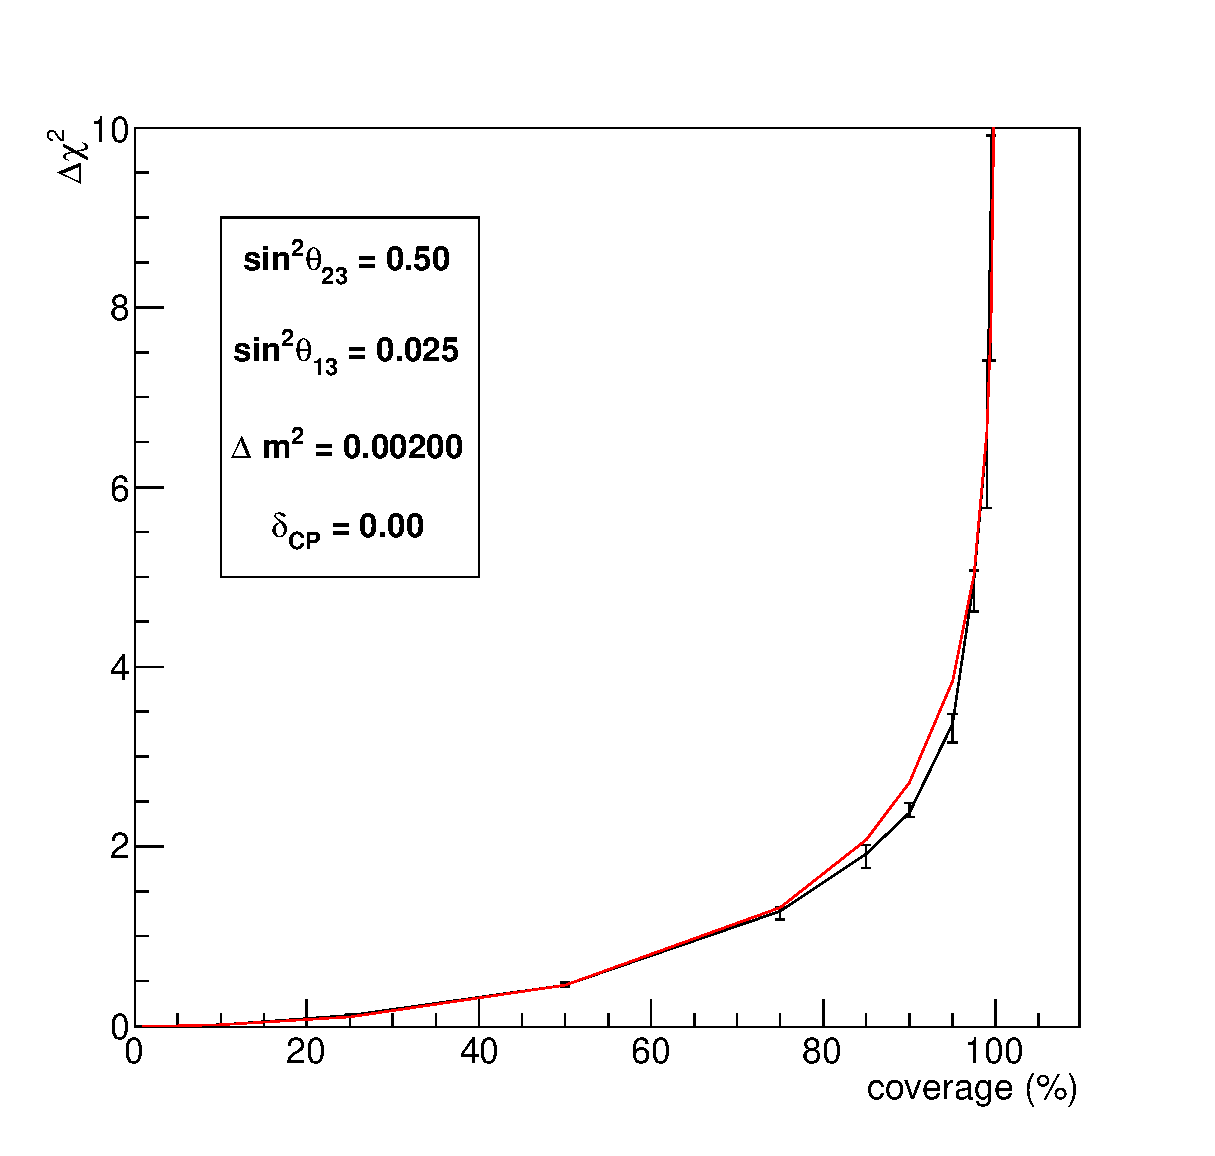
\includegraphics[width=14pc]{./images/appendix/coverage/coverage_study_1D_dm23sq_0.eps}
\center
\caption {
  Distribution of $\Delta\chi^{2}$ vs coverage in the $|\Delta m^{2}|$ parameter space
  from 1k toy MC experiments generated with the Run 1+2+3 POT
  with statistical fluctuations at the oscillation point indicated in the legend.
}
\label{fig:cov_1D_dmsq_0}
\end{minipage}
\hspace{0.03\linewidth}
\begin{minipage}[t]{0.46\linewidth}
\center
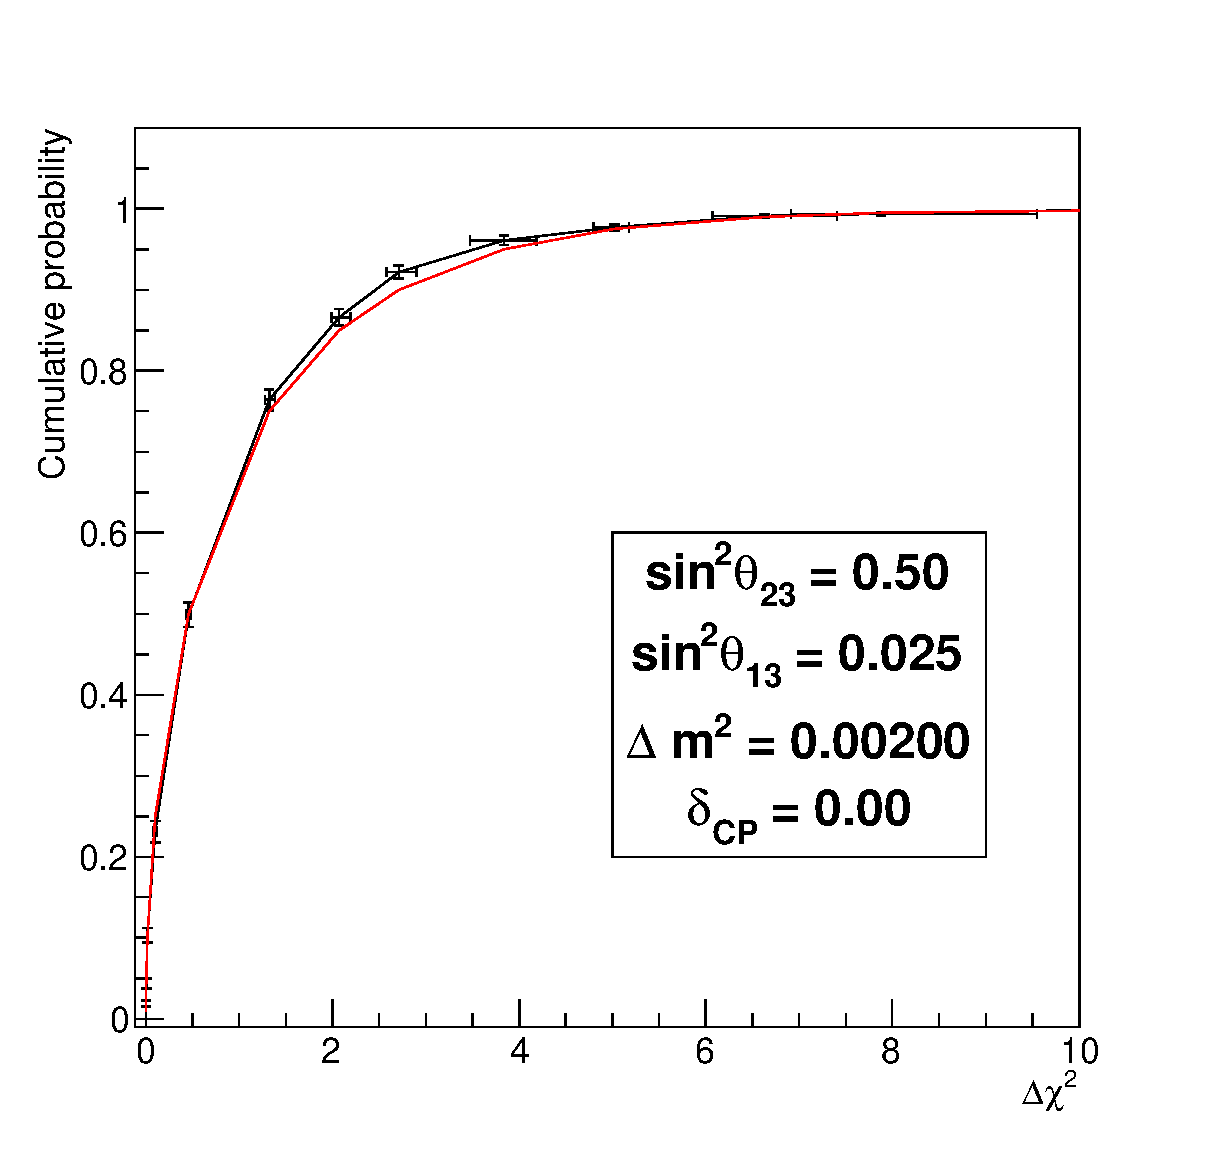
\includegraphics[width=14pc]{./images/appendix/coverage/coverage_study_1D_stats_dmsq_new_0.eps}
\center
\caption {
   Distribution of cumulative probability vs $\Delta\chi^{2}$ in the $|\Delta m^{2}|$ parameter space
  from 1k toy MC experiments generated with the Run 1+2+3 POT
  with statistical fluctuations at the oscillation point indicated in the legend.
	}
\label{fig:prob_1D_dmsq_0}
\end{minipage}
\vfill
\vspace*{0.7cm}
\begin{minipage}[t]{0.46\linewidth}
\center
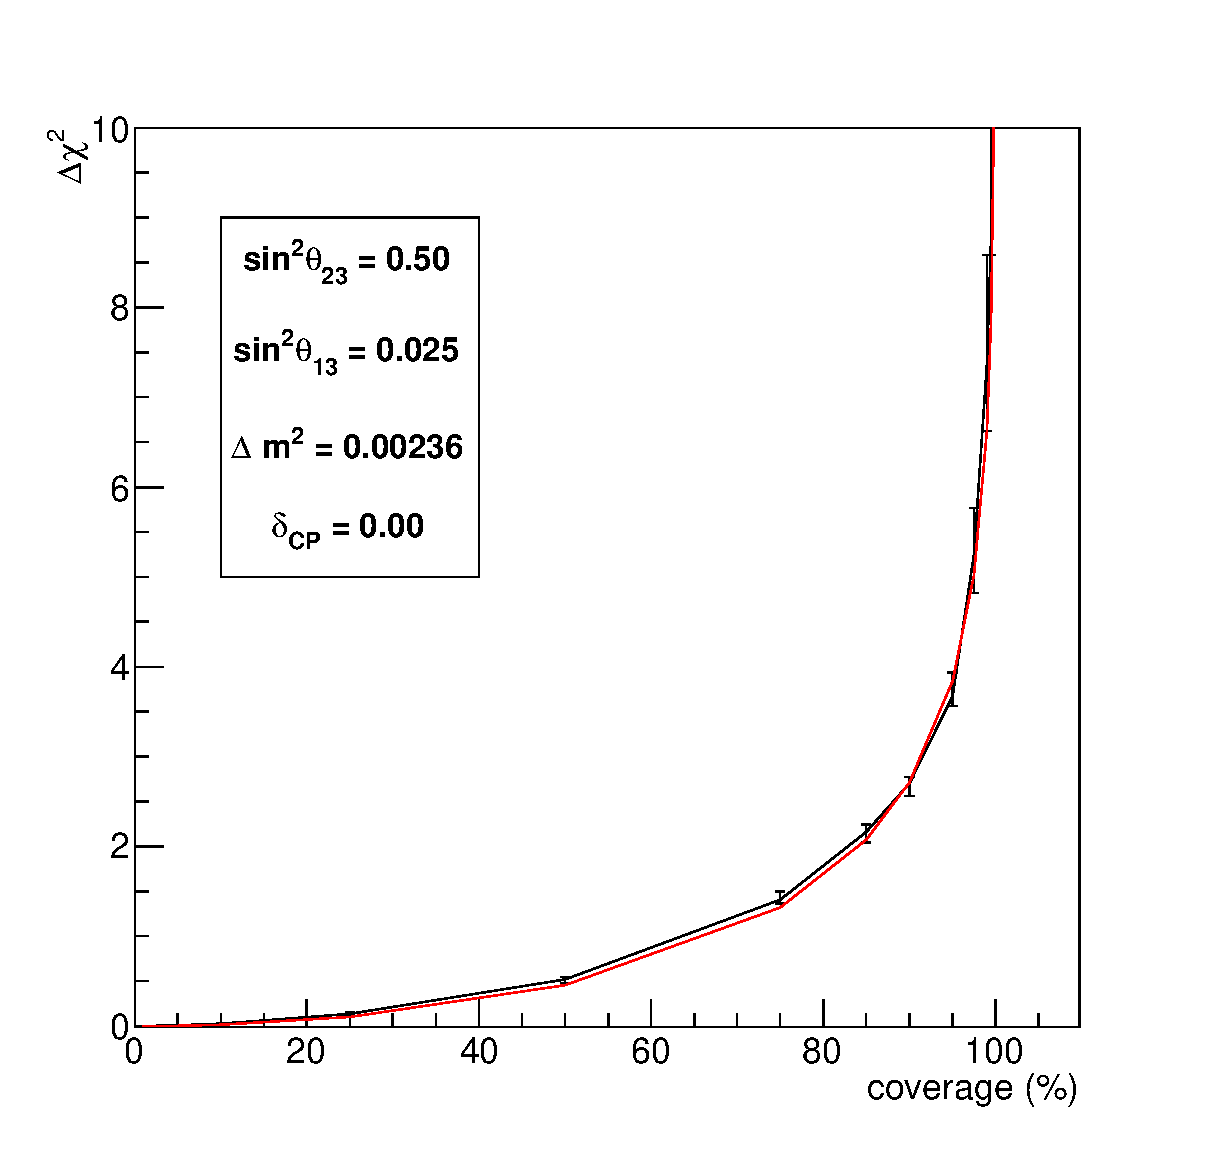
\includegraphics[width=14pc]{./images/appendix/coverage/coverage_study_1D_dm23sq_1.eps}
\center
\caption {
  Distribution of $\Delta\chi^{2}$ vs coverage in the $|\Delta m^{2}|$ parameter space
  from 1k toy MC experiments generated with the Run 1+2+3 POT
  with statistical fluctuations at the oscillation point indicated in the legend.
}
\label{fig:cov_1D_dmsq_1}
\end{minipage}
\hspace{0.03\linewidth}
\begin{minipage}[t]{0.46\linewidth}
\center
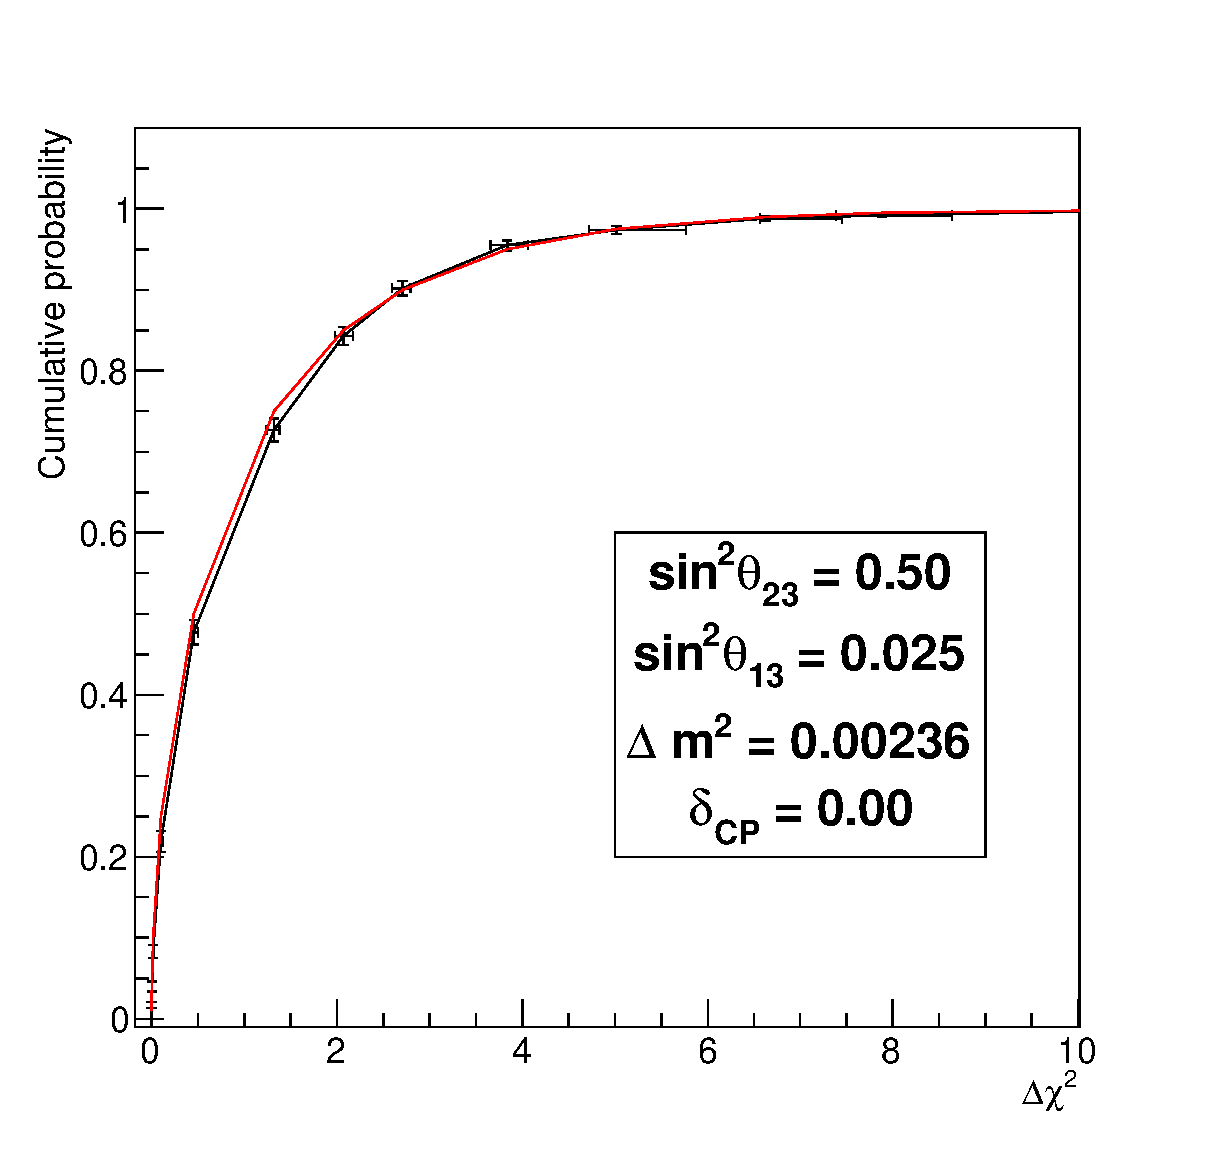
\includegraphics[width=14pc]{./images/appendix/coverage/coverage_study_1D_stats_dmsq_new_1.eps}
\center
\caption {
   Distribution of cumulative probability vs $\Delta\chi^{2}$ in the $|\Delta m^{2}|$ parameter space
  from 1k toy MC experiments generated with the Run 1+2+3 POT
  with statistical fluctuations at the oscillation point indicated in the legend.
	}
\label{fig:prob_1D_dmsq_1}
\end{minipage}
\vfill
\vspace*{0.7cm}
\begin{minipage}[t]{0.46\linewidth}
\center
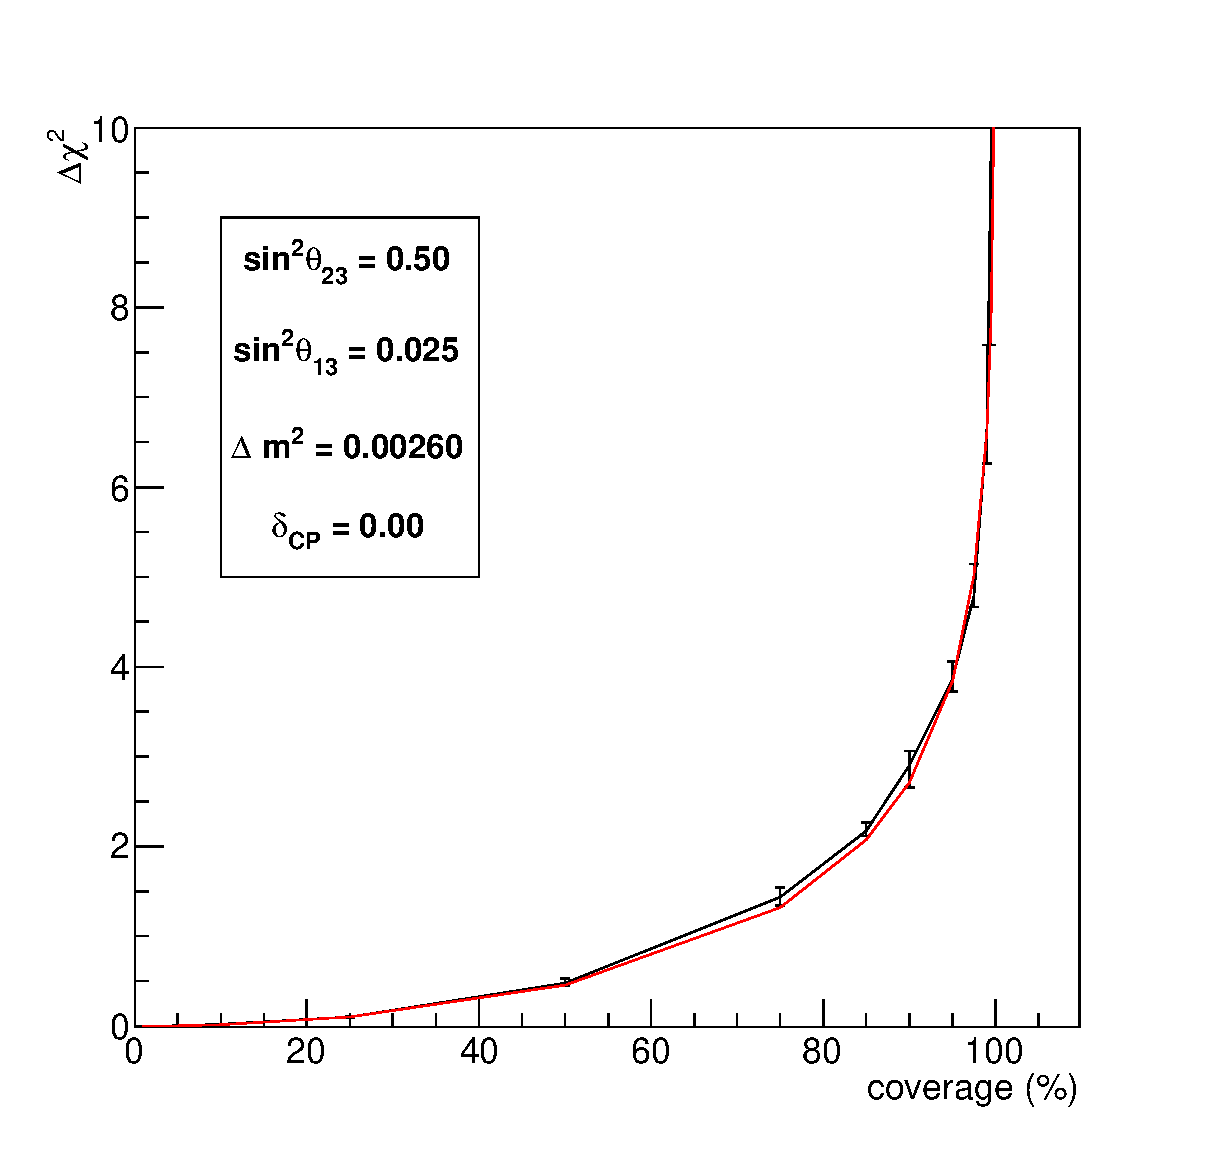
\includegraphics[width=14pc]{./images/appendix/coverage/coverage_study_1D_dm23sq_2.eps}
\center
\caption {
  Distribution of $\Delta\chi^{2}$ vs coverage in the $|\Delta m^{2}|$ parameter space
  from 1k toy MC experiments generated with the Run 1+2+3 POT
  with statistical fluctuations at the oscillation point indicated in the legend.
}
\label{fig:cov_1D_dmsq_2}
\end{minipage}
\hspace{0.03\linewidth}
\begin{minipage}[t]{0.46\linewidth}
\center
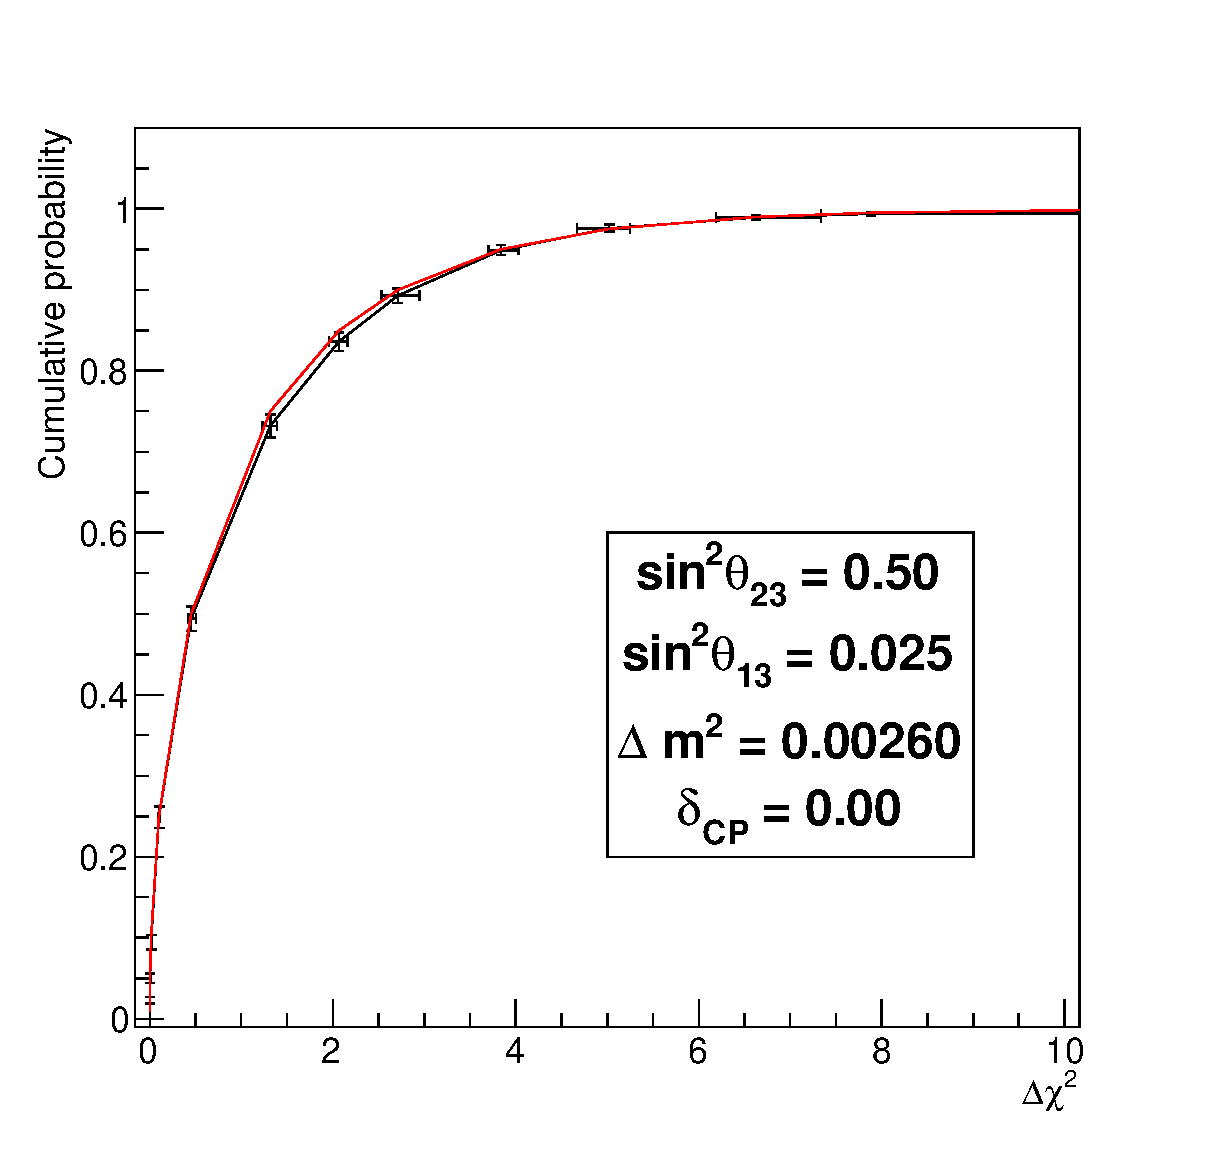
\includegraphics[width=14pc]{./images/appendix/coverage/coverage_study_1D_stats_dmsq_new_2.eps}
\center
\caption {
   Distribution of cumulative probability vs $\Delta\chi^{2}$ in the $|\Delta m^{2}|$ parameter space
  from 1k toy MC experiments generated with the Run 1+2+3 POT
  with statistical fluctuations at the oscillation point indicated in the legend.
	}
\label{fig:prob_1D_dmsq_2}
\end{minipage}
\end{figure*}
\end{center}
\begin{center}
\begin{figure*}[htb]
\begin{minipage}[t]{0.46\linewidth}
\center
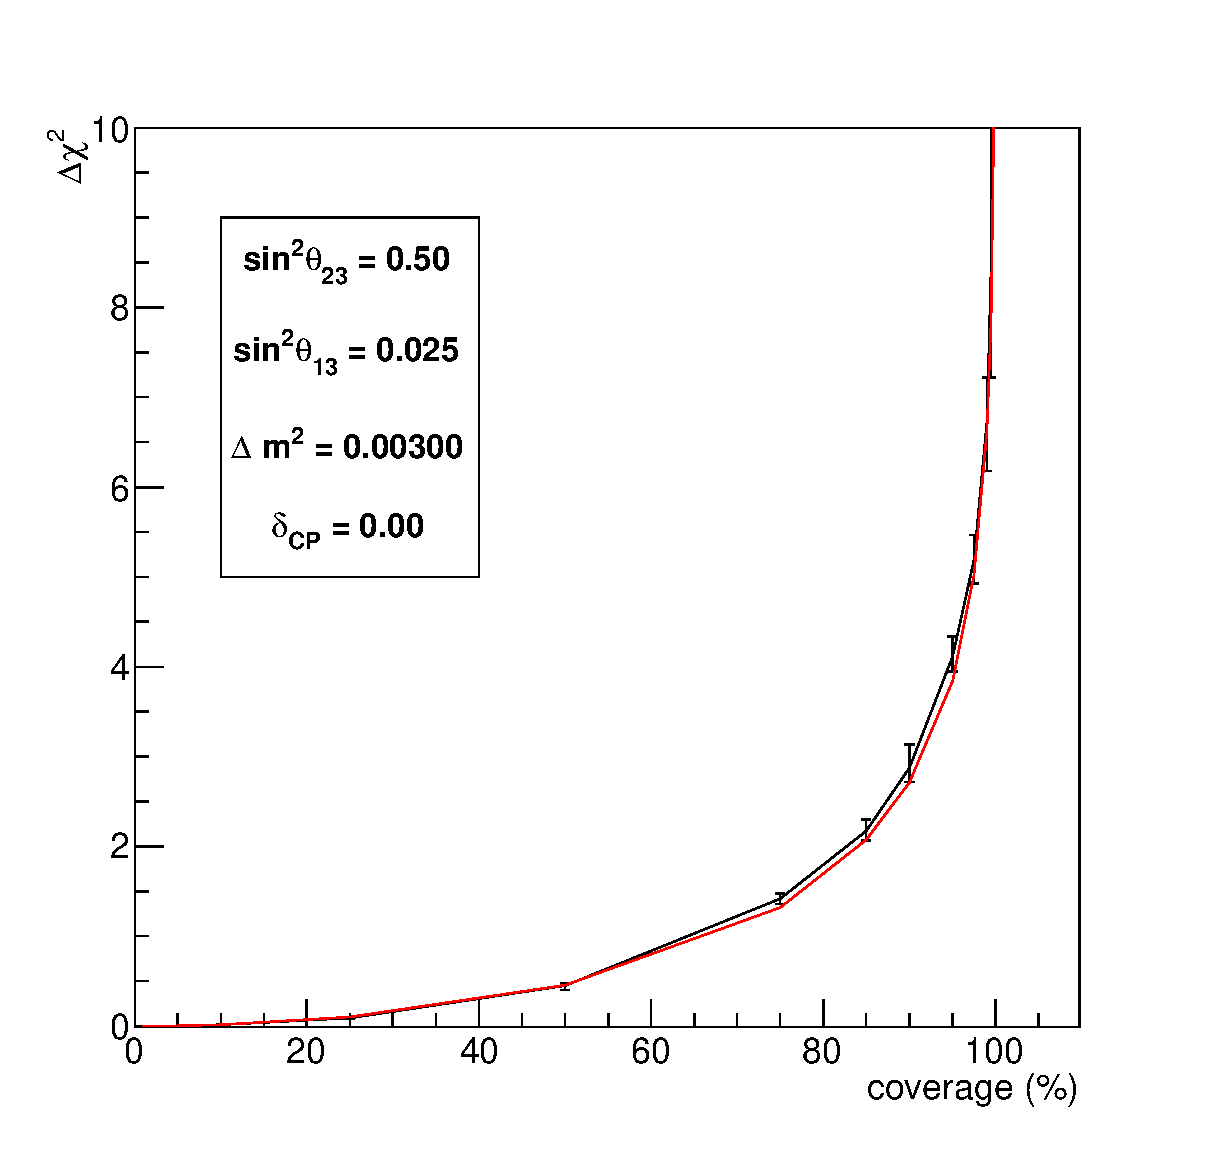
\includegraphics[width=14pc]{./images/appendix/coverage/coverage_study_1D_dm23sq_3.eps}
\center
\caption {
  Distribution of $\Delta\chi^{2}$ vs coverage in the $|\Delta m^{2}|$ parameter space
  from 1k toy MC experiments generated with the Run 1+2+3 POT
  with statistical fluctuations at the oscillation point indicated in the legend.
}
\label{fig:cov_1D_dmsq_3}
\end{minipage}
\hspace{0.03\linewidth}
\begin{minipage}[t]{0.46\linewidth}
\center
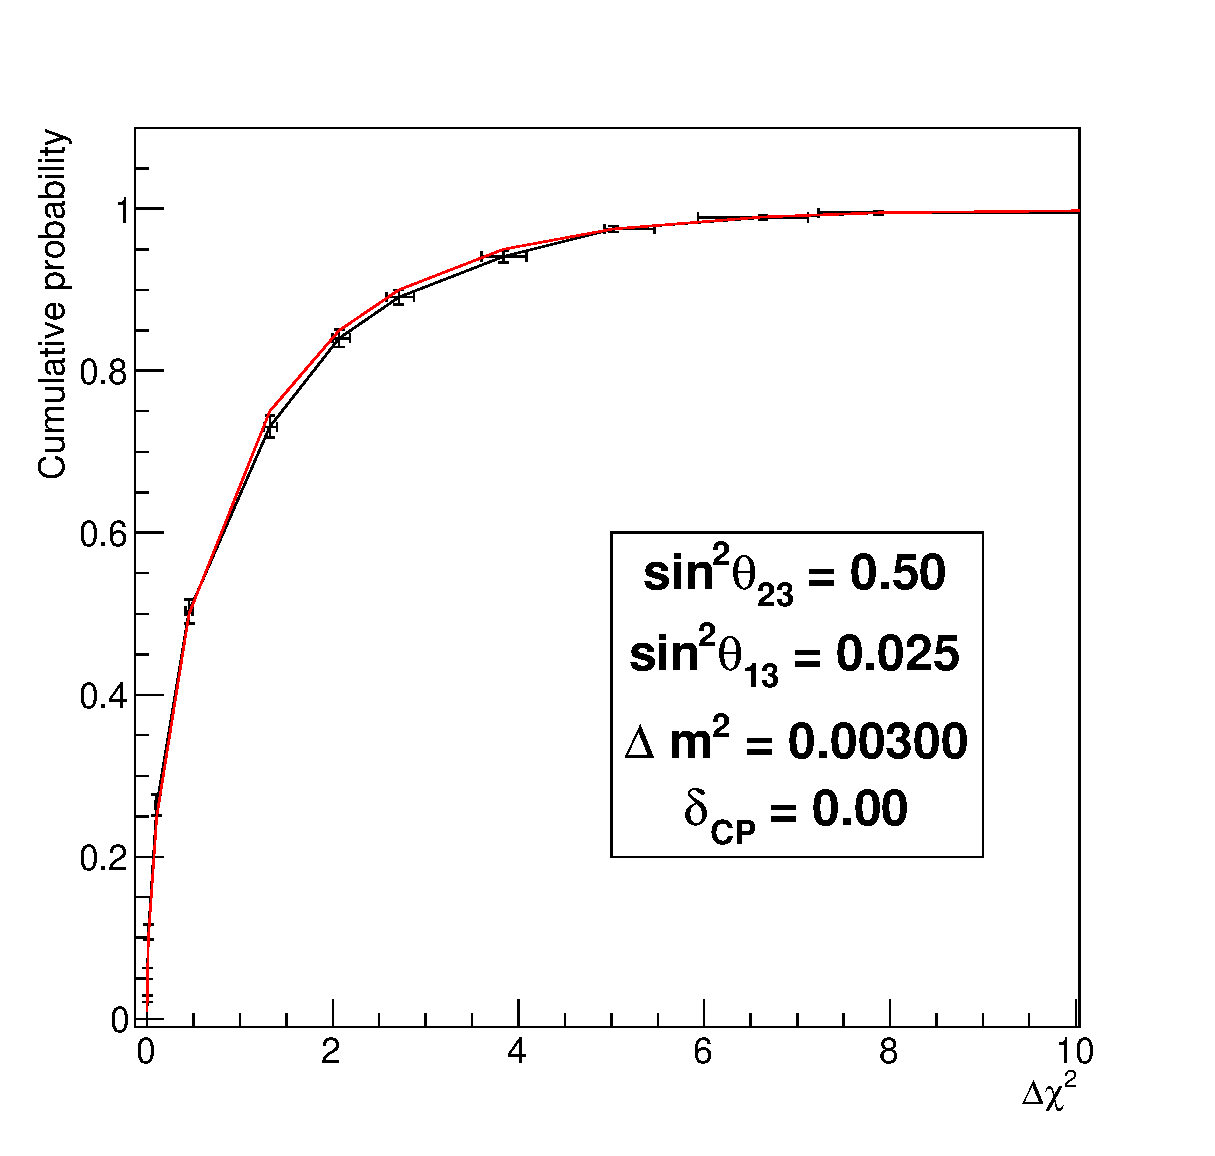
\includegraphics[width=14pc]{./images/appendix/coverage/coverage_study_1D_stats_dmsq_new_3.eps}
\center
\caption {
   Distribution of cumulative probability vs $\Delta\chi^{2}$ in the $|\Delta m^{2}|$ parameter space
  from 1k toy MC experiments generated with the Run 1+2+3 POT
  with statistical fluctuations at the oscillation point indicated in the legend.
	}
\label{fig:prob_1D_dmsq_3}
\end{minipage}
\vfill
\vspace*{0.7cm}
\begin{minipage}[t]{0.46\linewidth}
\center
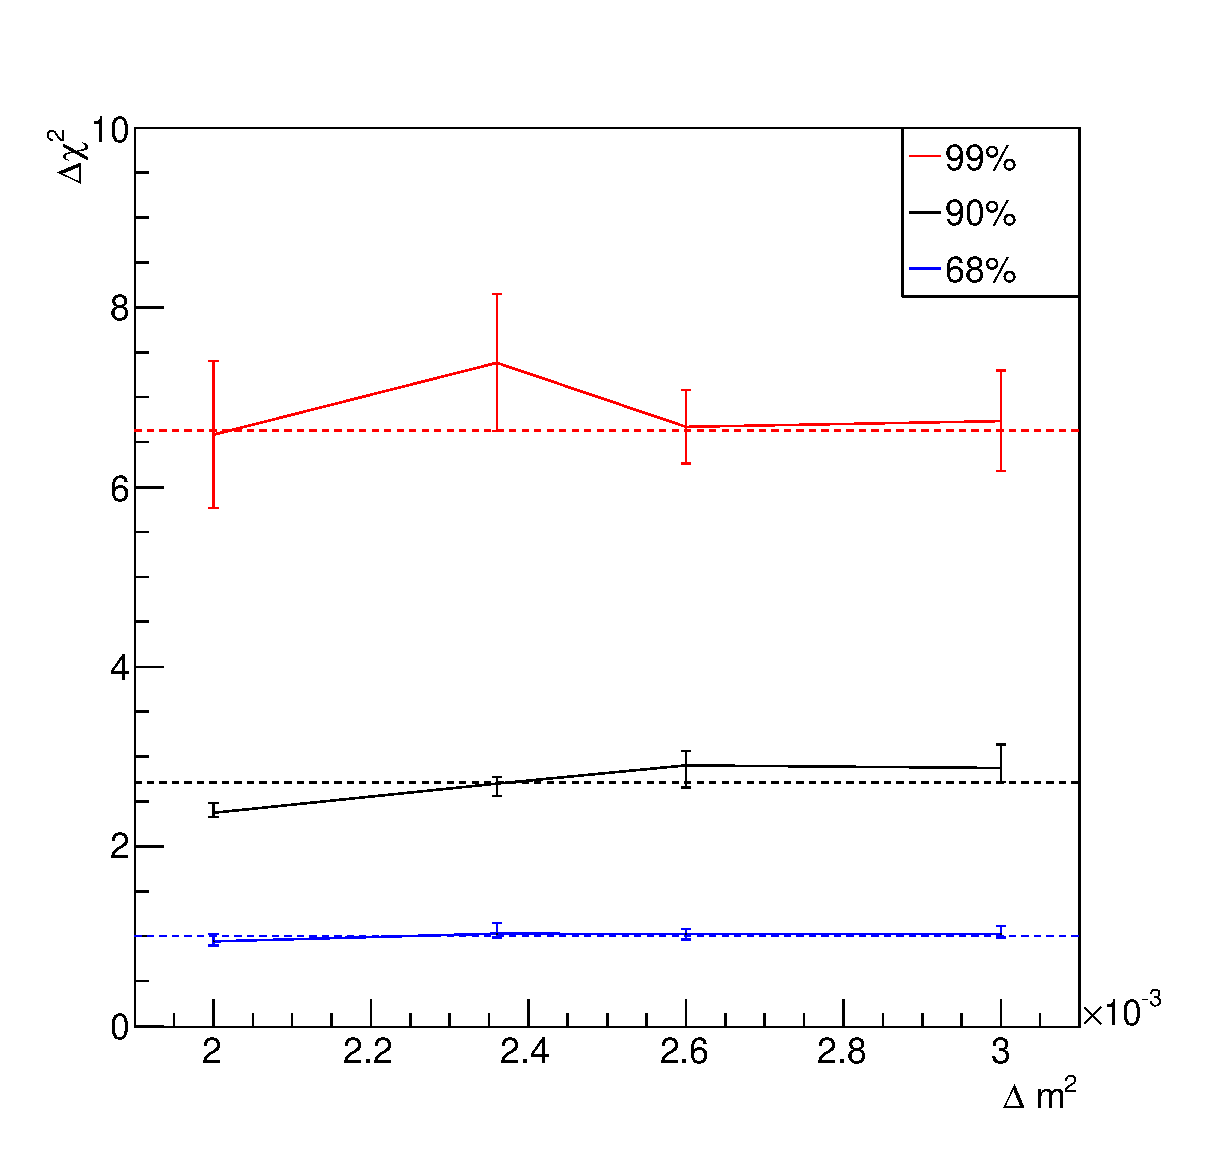
\includegraphics[width=14pc]{./images/appendix/coverage/coverage_study_1D_dm23sq_all.eps}
\caption {
   Summary of figures \ref{fig:cov_1D_dmsq_0}-\ref{fig:cov_1D_dmsq_3}
showing the value of $\Delta\chi^{2}$ at 99\%, 90\% and 68\% confidence intervals vs the value of $|\Delta m^{2}|$.
Horizontal dashed lines show the canonical $\Delta\chi^{2}$ value for 1 degree of freedom.
	}
\label{fig:prob_1D_dmsq_all}
\end{minipage}
\hspace{0.03\linewidth}
\begin{minipage}[t]{0.46\linewidth}
\center
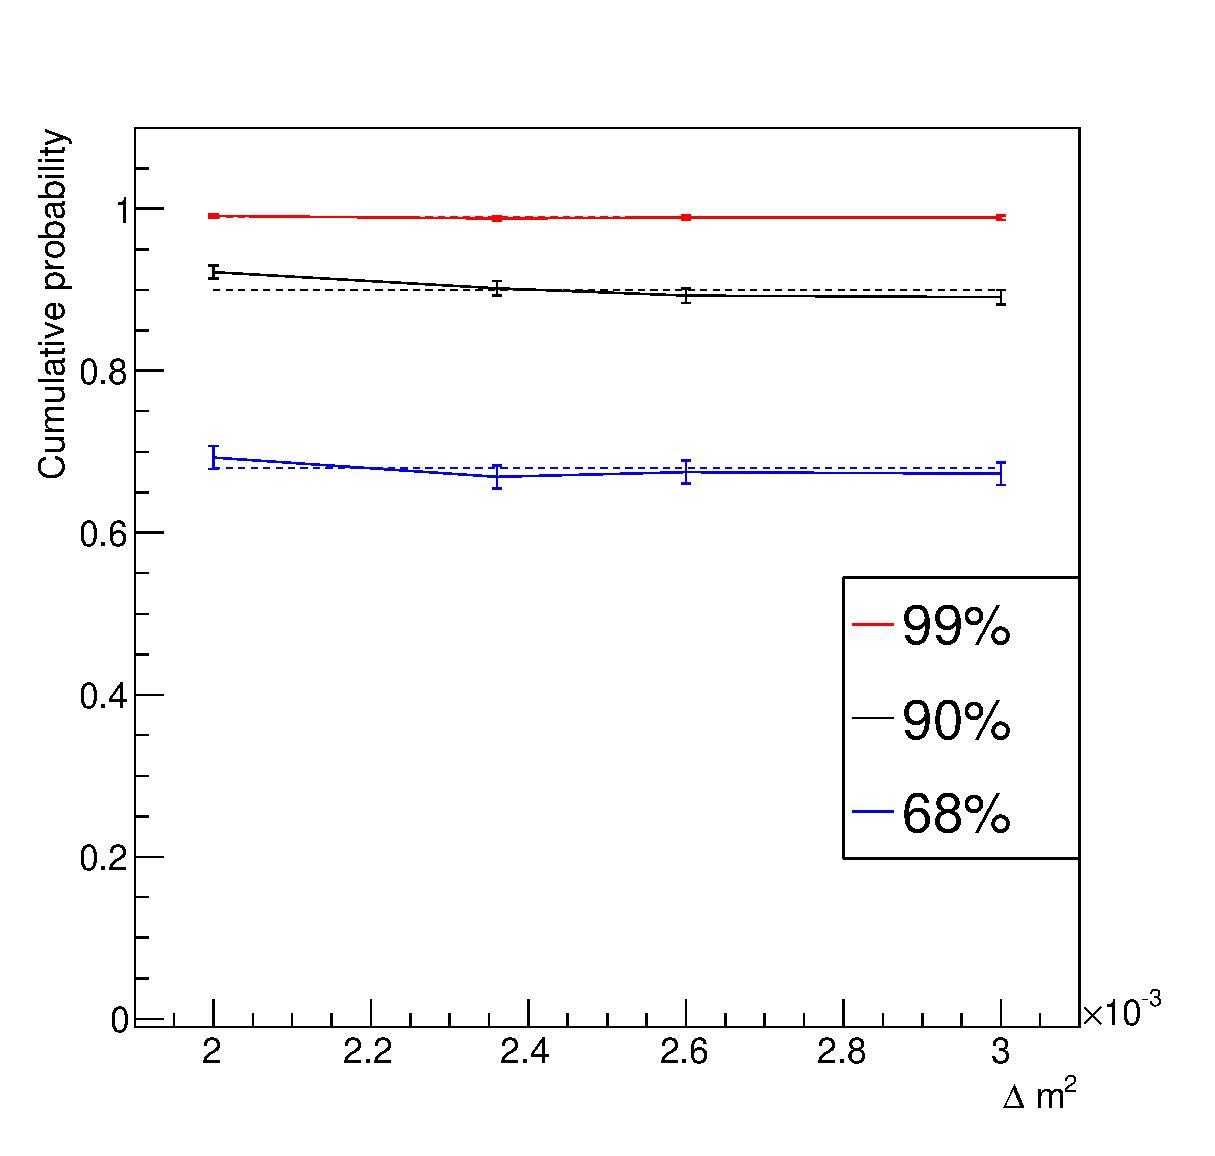
\includegraphics[width=14pc]{./images/appendix/coverage/coverage_study_1D_stats_dmsq_new_all.eps}
\caption {
   Summary of figures \ref{fig:prob_1D_dmsq_0}-\ref{fig:prob_1D_dmsq_3}
showing the value of cumulative probability for $\Delta\chi^{2}=6.63$ (canonical value for 99\%), $\Delta\chi^{2}=2.71$ (canonical value for 90\%) and $\Delta\chi^{2}=1.0$ (canonical value for 68\%) vs the value of $|\Delta m^{2}|$.
}
\label{fig:cov_1D_dmsq_all}
\end{minipage}
\end{figure*}
\end{center}

%% FIGURES FOR 1D theta23

\begin{center}
\begin{figure*}[htb]
\begin{minipage}[t]{0.46\linewidth}
\center
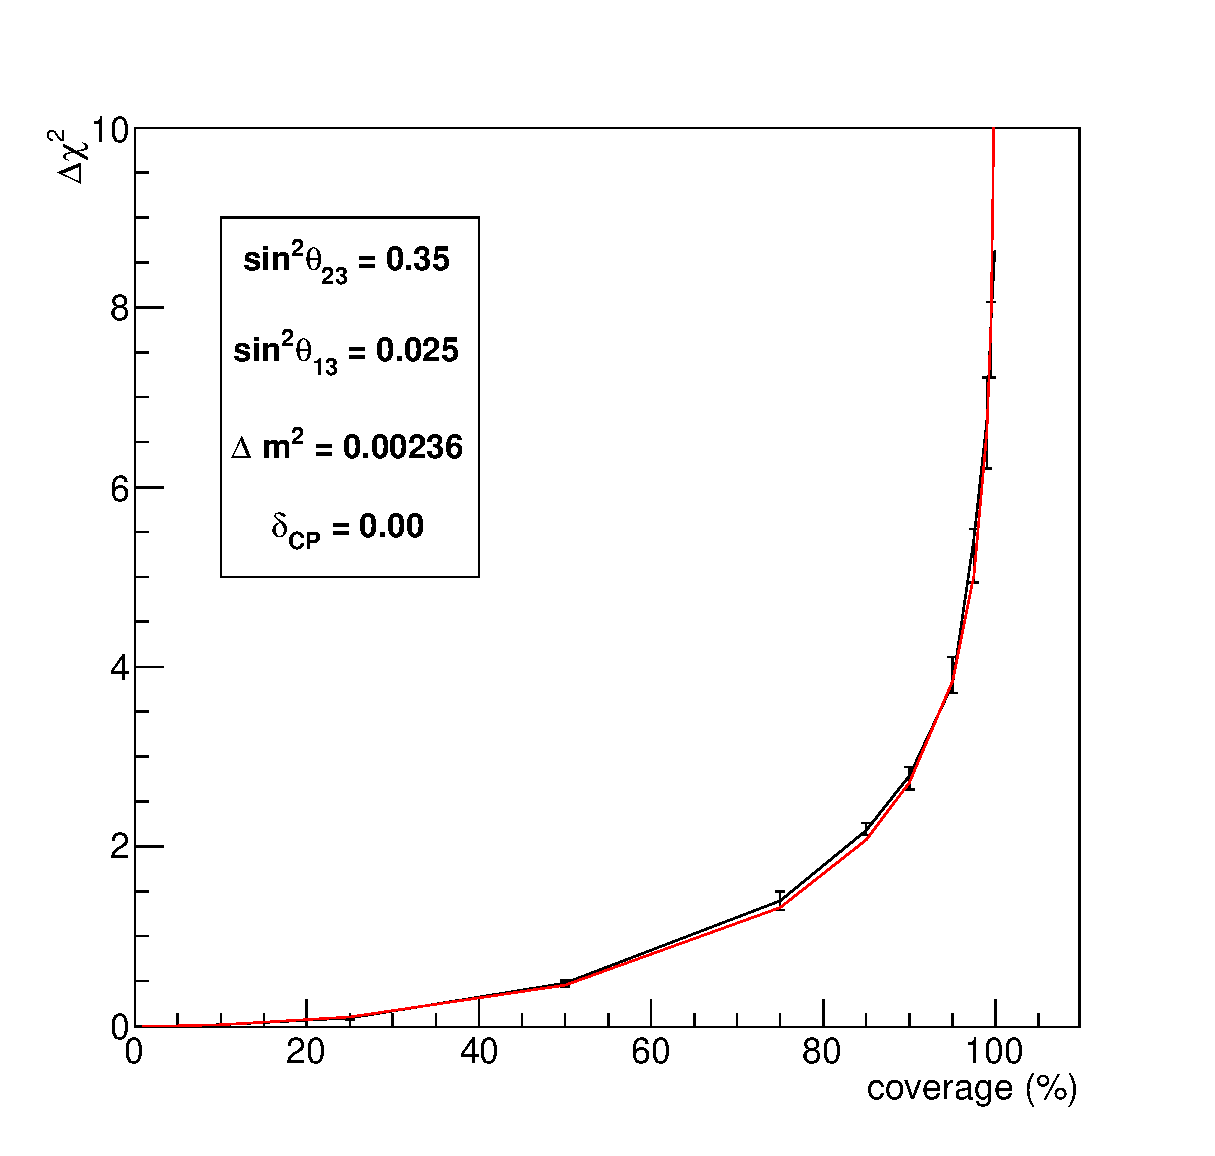
\includegraphics[width=14pc]{./images/appendix/coverage/coverage_study_1D_theta23_0.eps}
\center
\caption {
  Distribution of $\Delta\chi^{2}$ vs coverage in the $sin^{2}\theta_{23}$ parameter space
  from 1k toy MC experiments generated with the Run 1+2+3 POT
  with statistical fluctuations at the oscillation point indicated in the legend.
}
\label{fig:cov_1D_theta23_0}
\end{minipage}
\hspace{0.03\linewidth}
\begin{minipage}[t]{0.46\linewidth}
\center
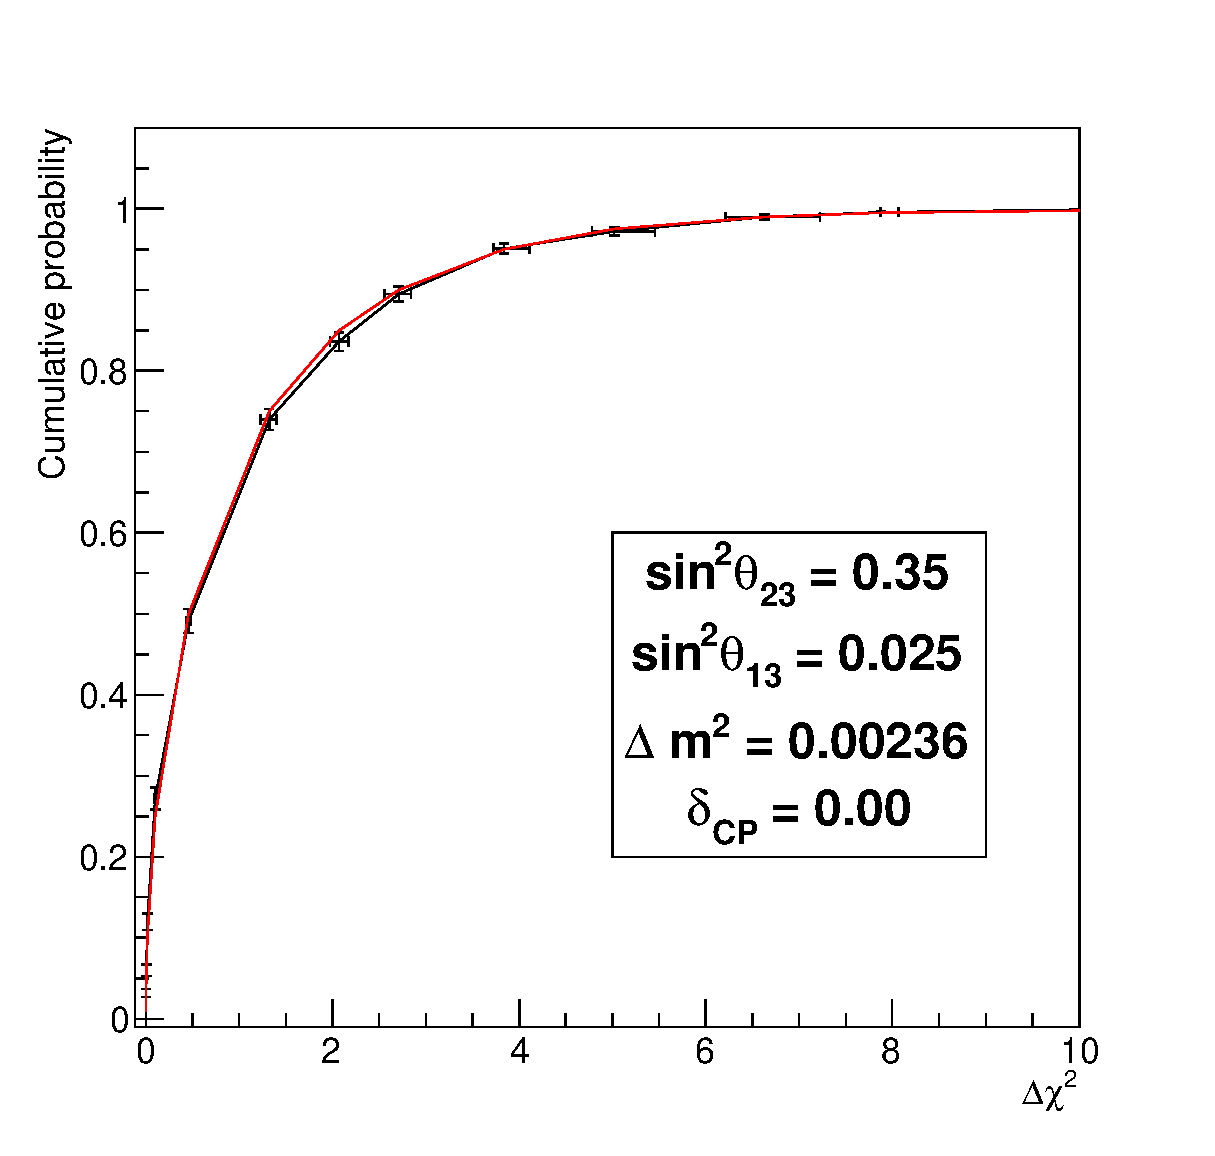
\includegraphics[width=14pc]{./images/appendix/coverage/coverage_study_1D_stats_theta23_new_0.eps}
\center
\caption {
  Distribution of cumulative probability vs $\Delta\chi^{2}$ in the $sin^{2}\theta_{23}$ parameter space
  from 1k toy MC experiments generated with the Run 1+2+3 POT
  with statistical fluctuations at the oscillation point indicated in the legend.
}
\label{fig:prob_1D_theta23_0}
\end{minipage}
\begin{minipage}[t]{0.46\linewidth}
\center
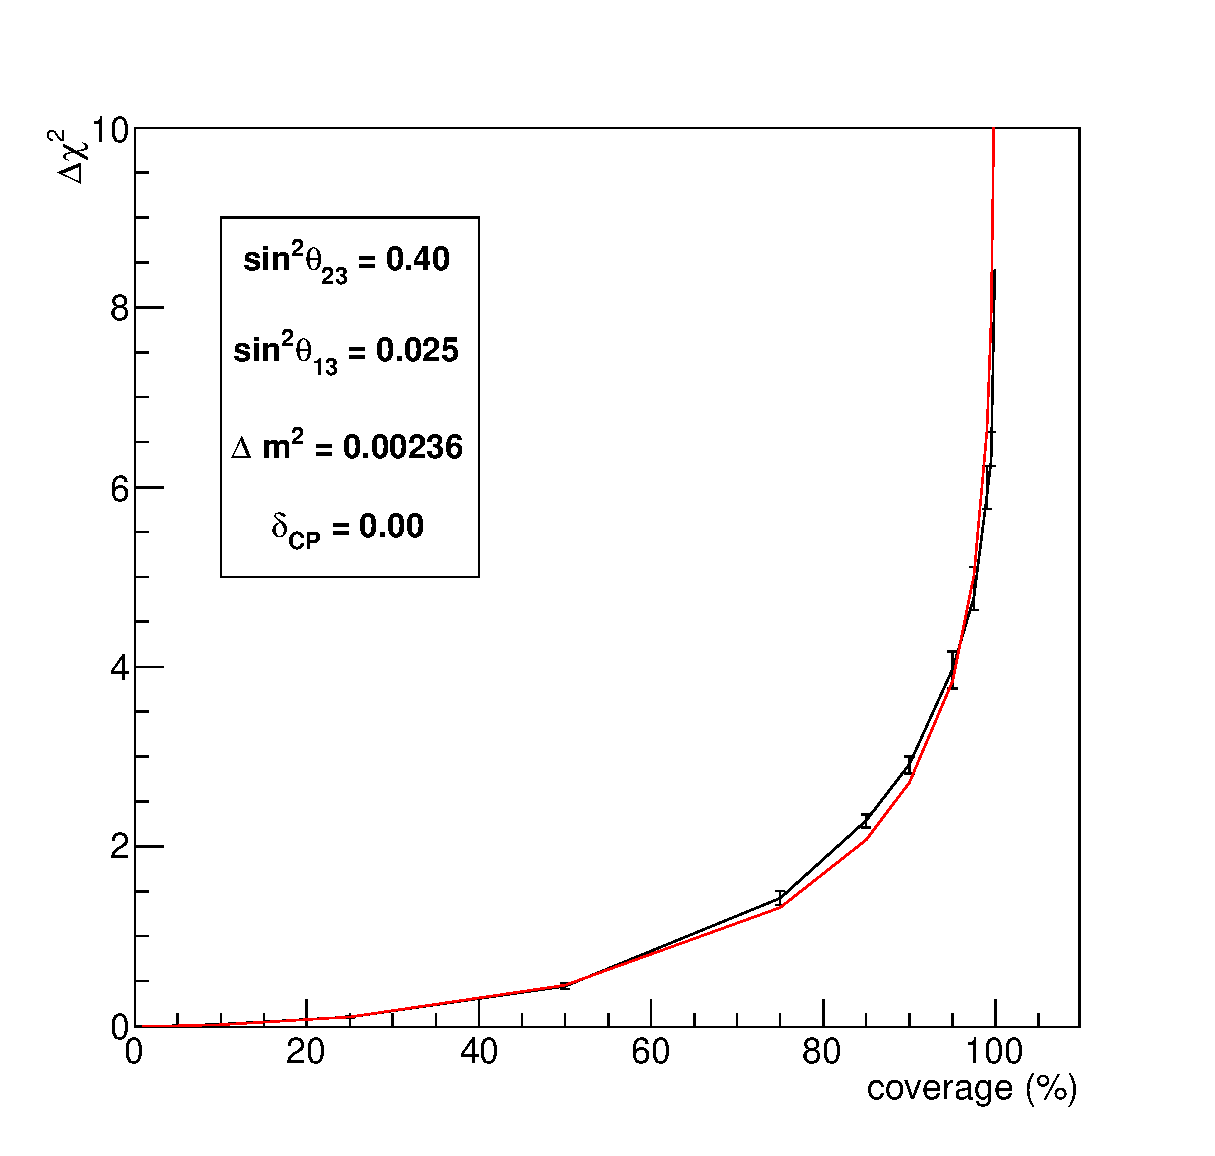
\includegraphics[width=14pc]{./images/appendix/coverage/coverage_study_1D_theta23_1.eps}
\center
\caption {
  Distribution of $\Delta\chi^{2}$ vs coverage in the $sin^{2}\theta_{23}$ parameter space
  from 1k toy MC experiments generated with the Run 1+2+3 POT
  with statistical fluctuations at the oscillation point indicated in the legend.
}
\label{fig:cov_1D_theta23_1}
\end{minipage}
\hspace{0.03\linewidth}
\begin{minipage}[t]{0.46\linewidth}
\center
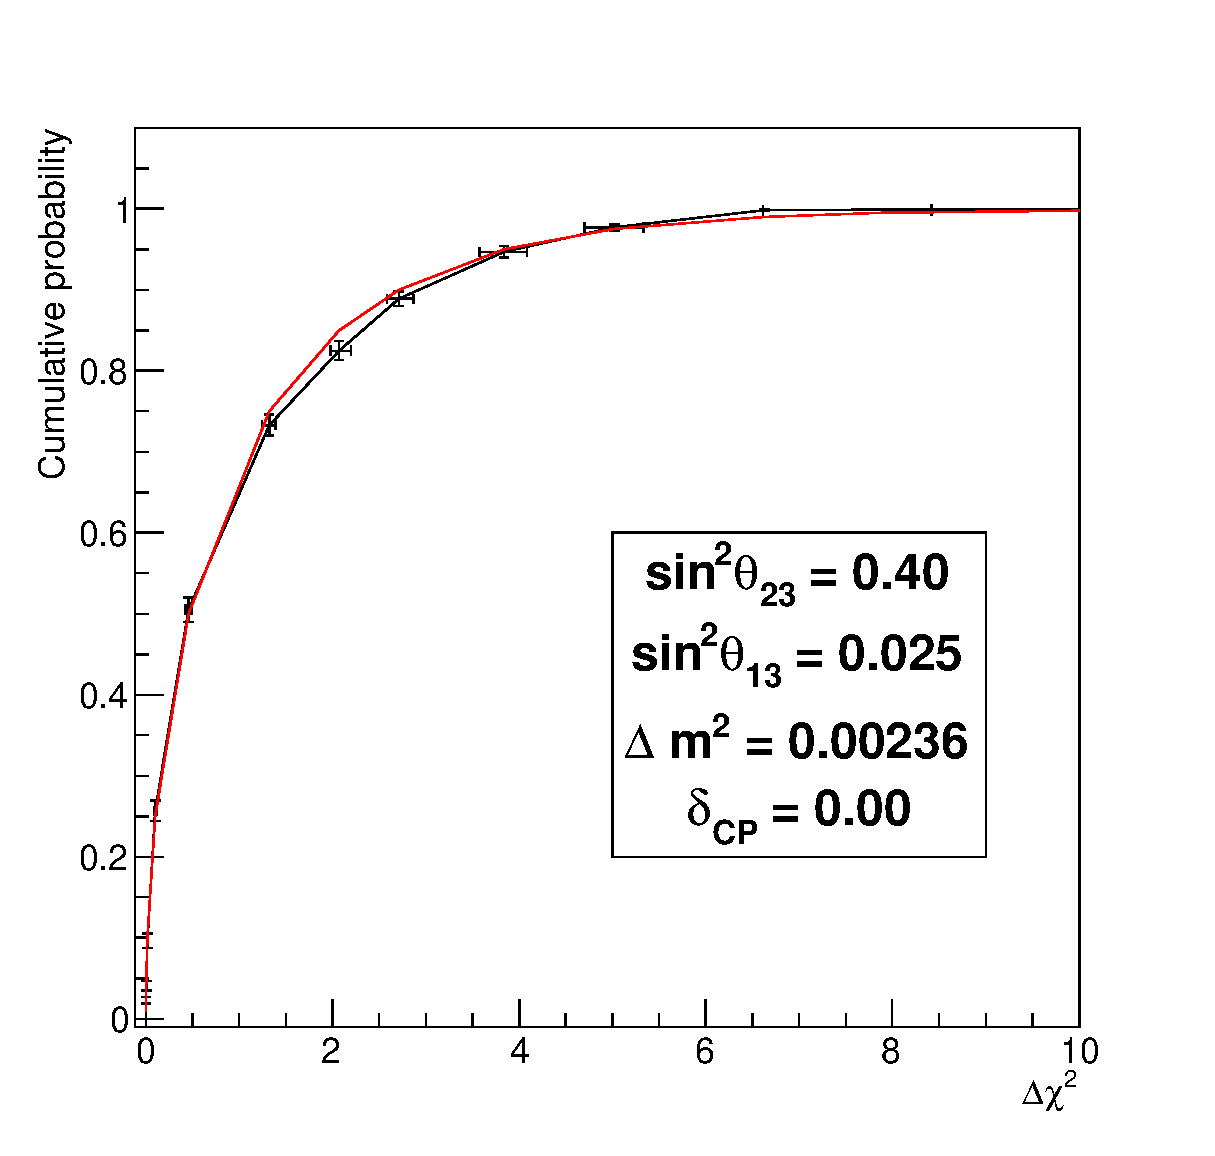
\includegraphics[width=14pc]{./images/appendix/coverage/coverage_study_1D_stats_theta23_new_1.eps}
\center
\caption {
  Distribution of cumulative probability vs $\Delta\chi^{2}$ in the $sin^{2}\theta_{23}$ parameter space
  from 1k toy MC experiments generated with the Run 1+2+3 POT
  with statistical fluctuations at the oscillation point indicated in the legend.
}
\label{fig:prob_1D_theta23_1}
\end{minipage}
\vfill
\vspace*{0.7cm}
\begin{minipage}[t]{0.46\linewidth}
\center
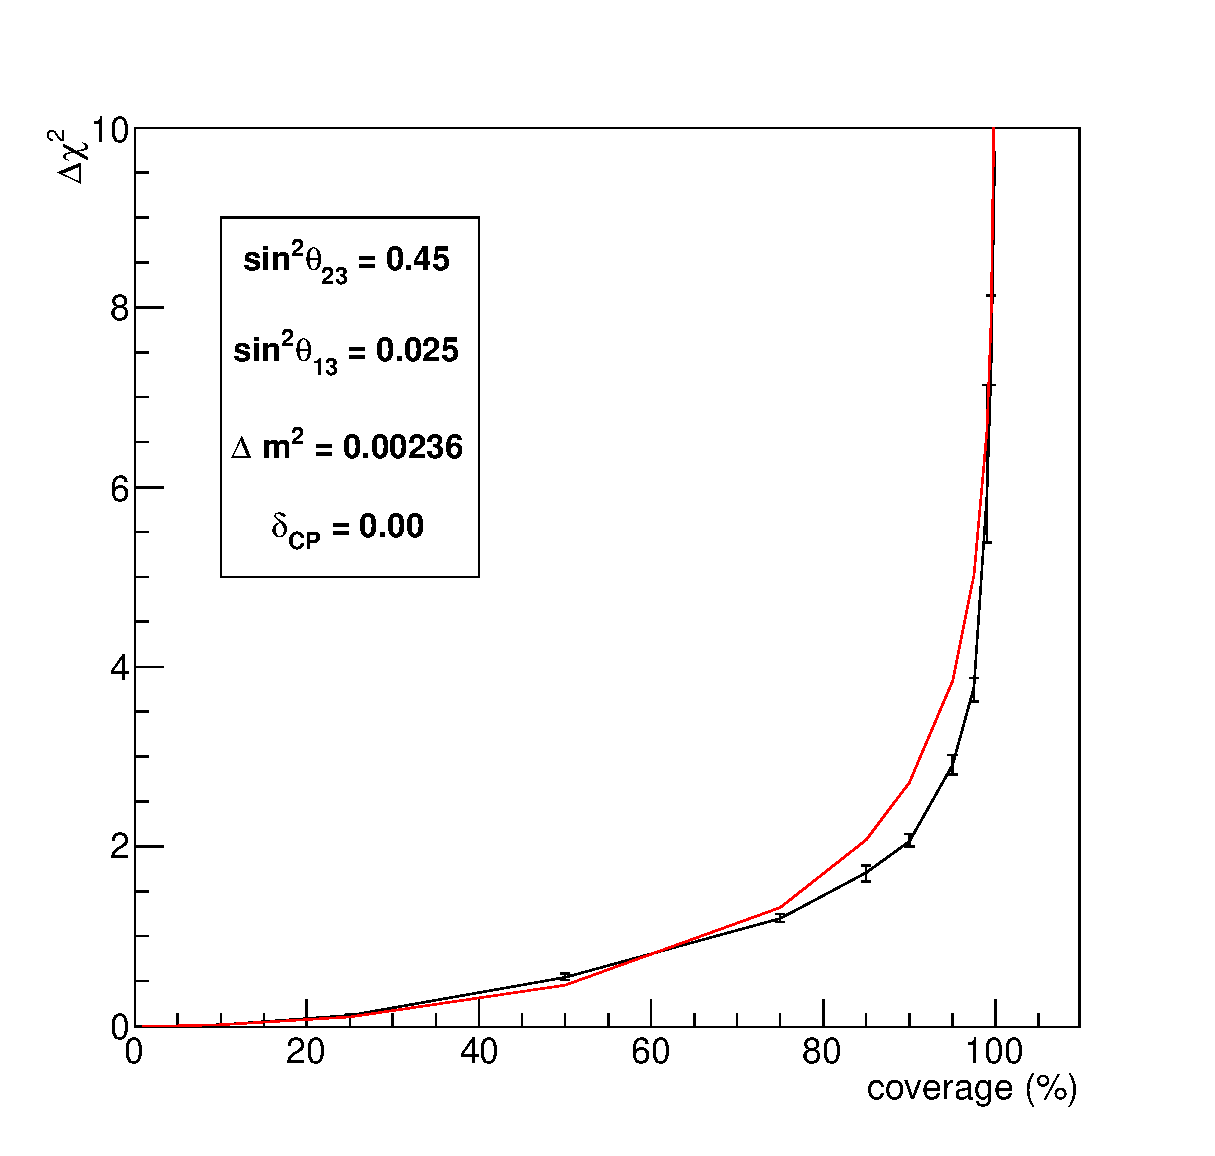
\includegraphics[width=14pc]{./images/appendix/coverage/coverage_study_1D_theta23_2.eps}
\center
\caption {
  Distribution of $\Delta\chi^{2}$ vs coverage in the $sin^{2}\theta_{23}$ parameter space
  from 1k toy MC experiments generated with the Run 1+2+3 POT
  with statistical fluctuations at the oscillation point indicated in the legend.
}
\label{fig:cov_1D_theta23_2}
\end{minipage}
\hspace{0.03\linewidth}
\begin{minipage}[t]{0.46\linewidth}
\center
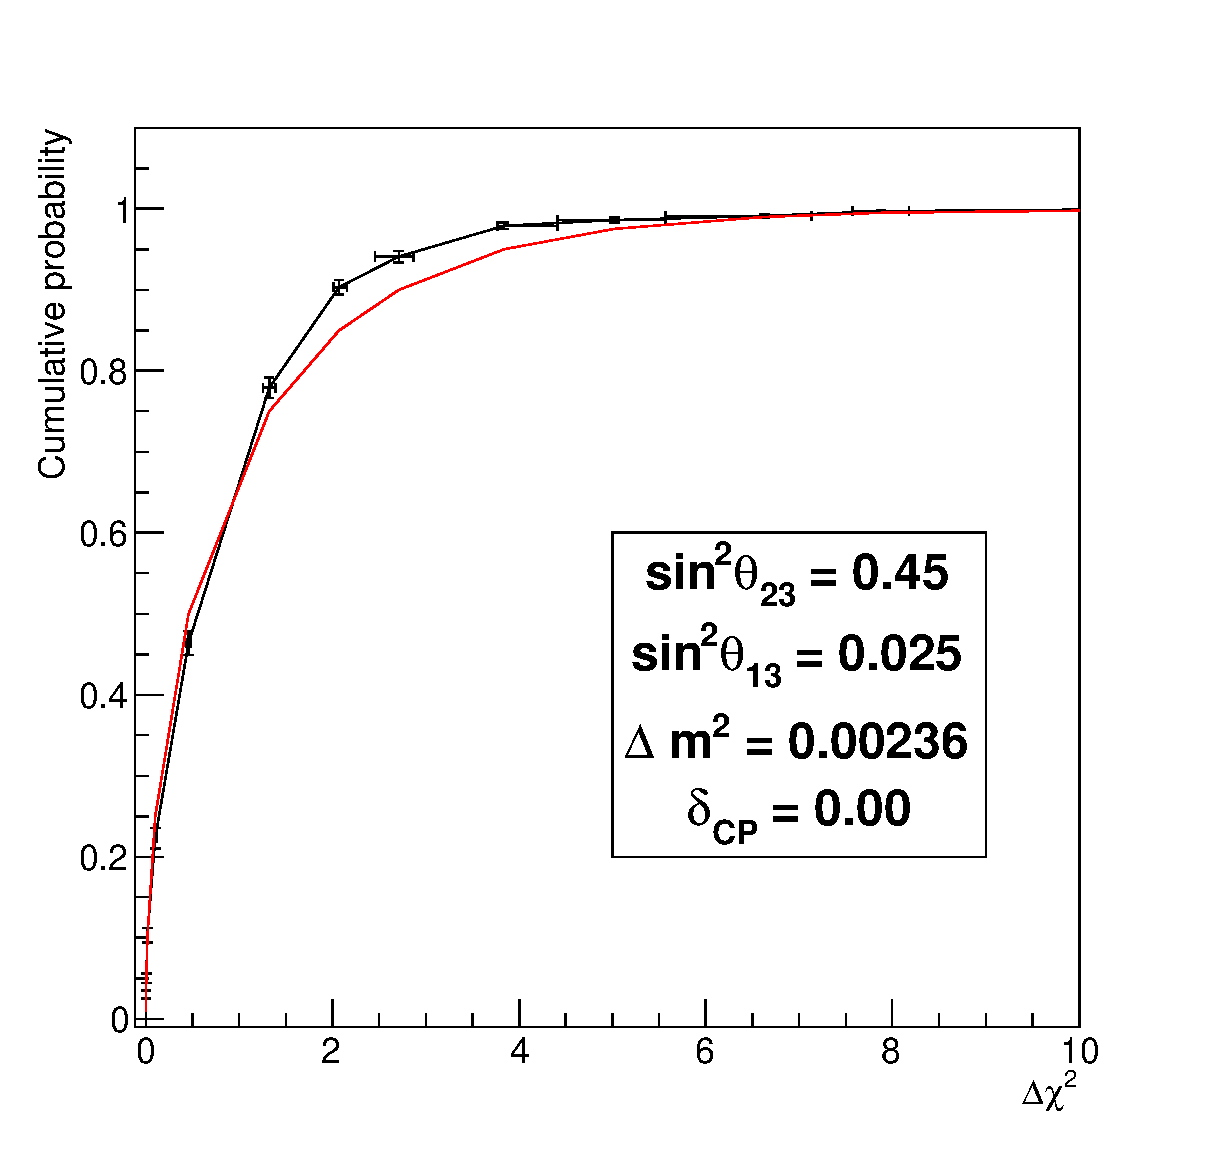
\includegraphics[width=14pc]{./images/appendix/coverage/coverage_study_1D_stats_theta23_new_2.eps}
\center
\caption {
  Distribution of cumulative probability vs $\Delta\chi^{2}$ in the $sin^{2}\theta_{23}$ parameter space
  from 1k toy MC experiments generated with the Run 1+2+3 POT
  with statistical fluctuations at the oscillation point indicated in the legend.
}
\label{fig:prod_1D_theta23_2}
\end{minipage}
\end{figure*}
\end{center}
\begin{center}
\begin{figure*}[htb]
\begin{minipage}[t]{0.46\linewidth}
\center
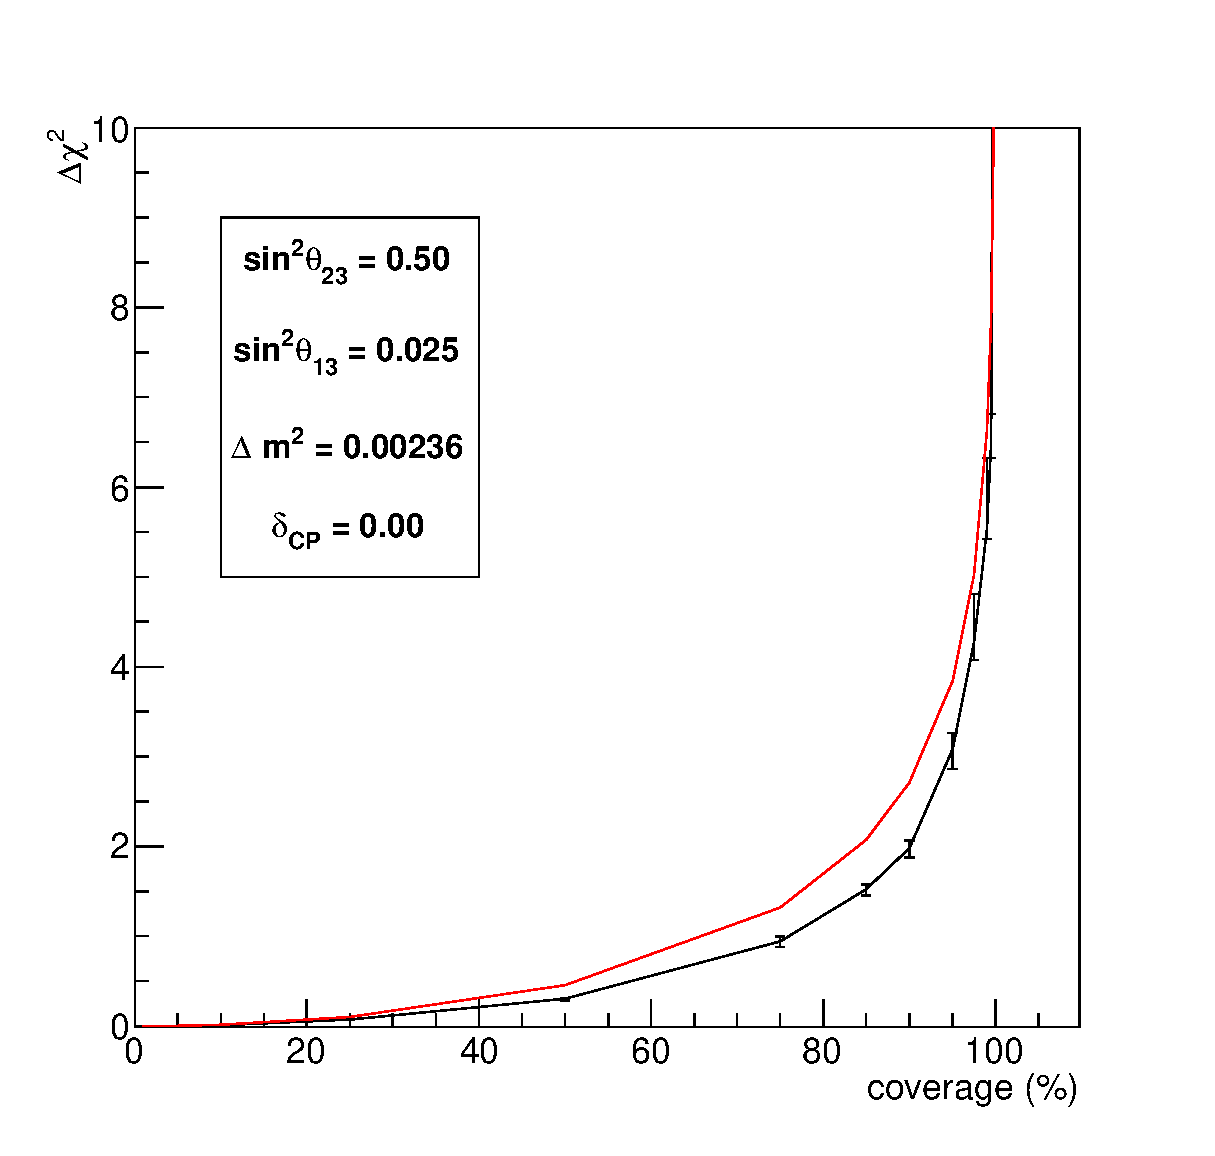
\includegraphics[width=14pc]{./images/appendix/coverage/coverage_study_1D_theta23_3.eps}
\center
\caption {
  Distribution of $\Delta\chi^{2}$ vs coverage in the $sin^{2}\theta_{23}$ parameter space
  from 1k toy MC experiments generated with the Run 1+2+3 POT
  with statistical fluctuations at the oscillation point indicated in the legend.
}
\label{fig:cov_1D_theta23_3}
\end{minipage}
\hspace{0.03\linewidth}
\begin{minipage}[t]{0.46\linewidth}
\center
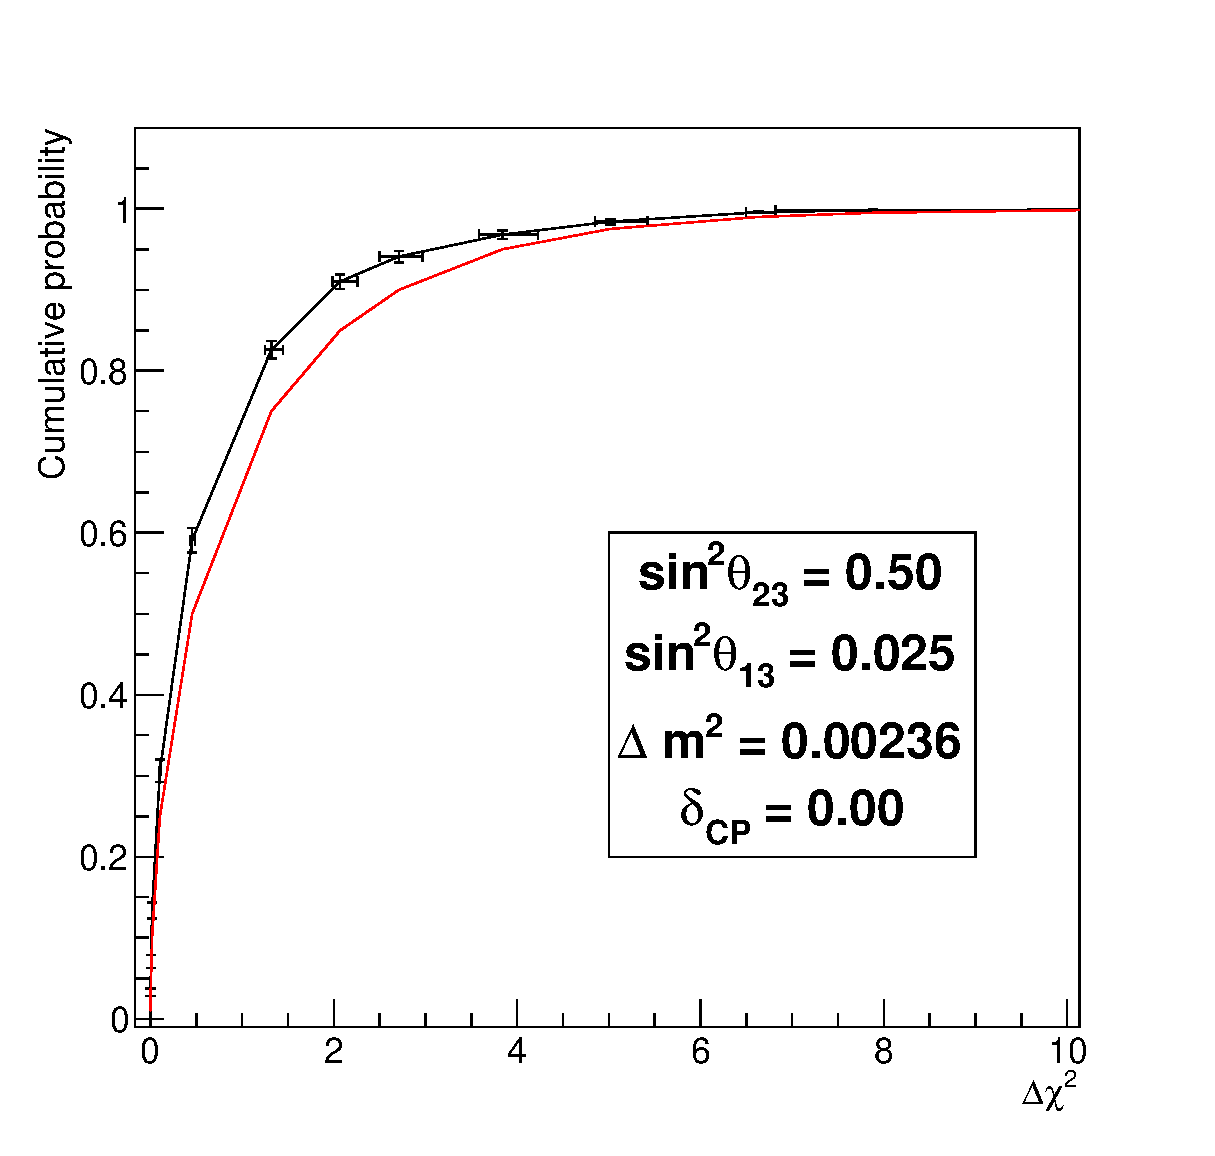
\includegraphics[width=14pc]{./images/appendix/coverage/coverage_study_1D_stats_theta23_new_3.eps}
\center
\caption {
  Distribution of cumulative probability vs $\Delta\chi^{2}$ in the $sin^{2}\theta_{23}$ parameter space
  from 1k toy MC experiments generated with the Run 1+2+3 POT
  with statistical fluctuations at the oscillation point indicated in the legend.
}
\label{fig:prob_1D_theta23_3}
\end{minipage}
\vfill
\vspace*{0.7cm}
\center
\begin{minipage}[t]{0.46\linewidth}
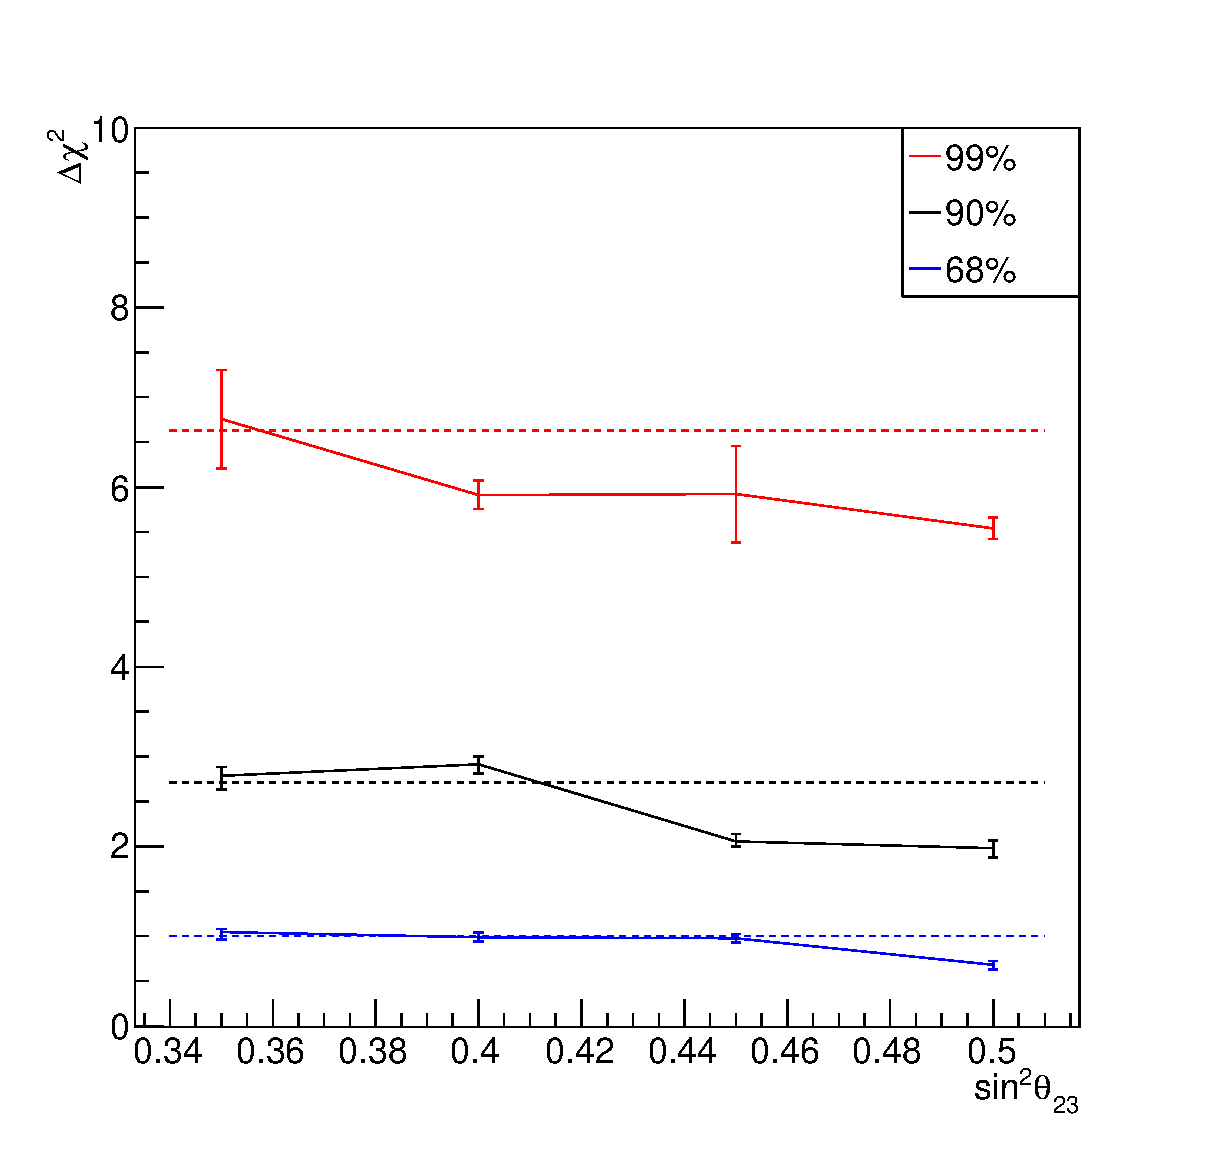
\includegraphics[width=14pc]{./images/appendix/coverage/coverage_study_1D_theta23_all.eps}
\caption {
   Summary of figures \ref{fig:cov_1D_theta23_0}-\ref{fig:cov_1D_theta23_3}
showing the value of $\Delta\chi^{2}$ at 99\%, 90\% and 68\% confidence intervals vs the value of $sin^{2}\theta_{23}$.
Horizontal dashed lines show the canonical $\Delta\chi^{2}$ value for 1 degree of freedom.
	}
\label{fig:cov_1D_theta23_all}
\end{minipage}
\hspace{0.03\linewidth}
\begin{minipage}[t]{0.46\linewidth}
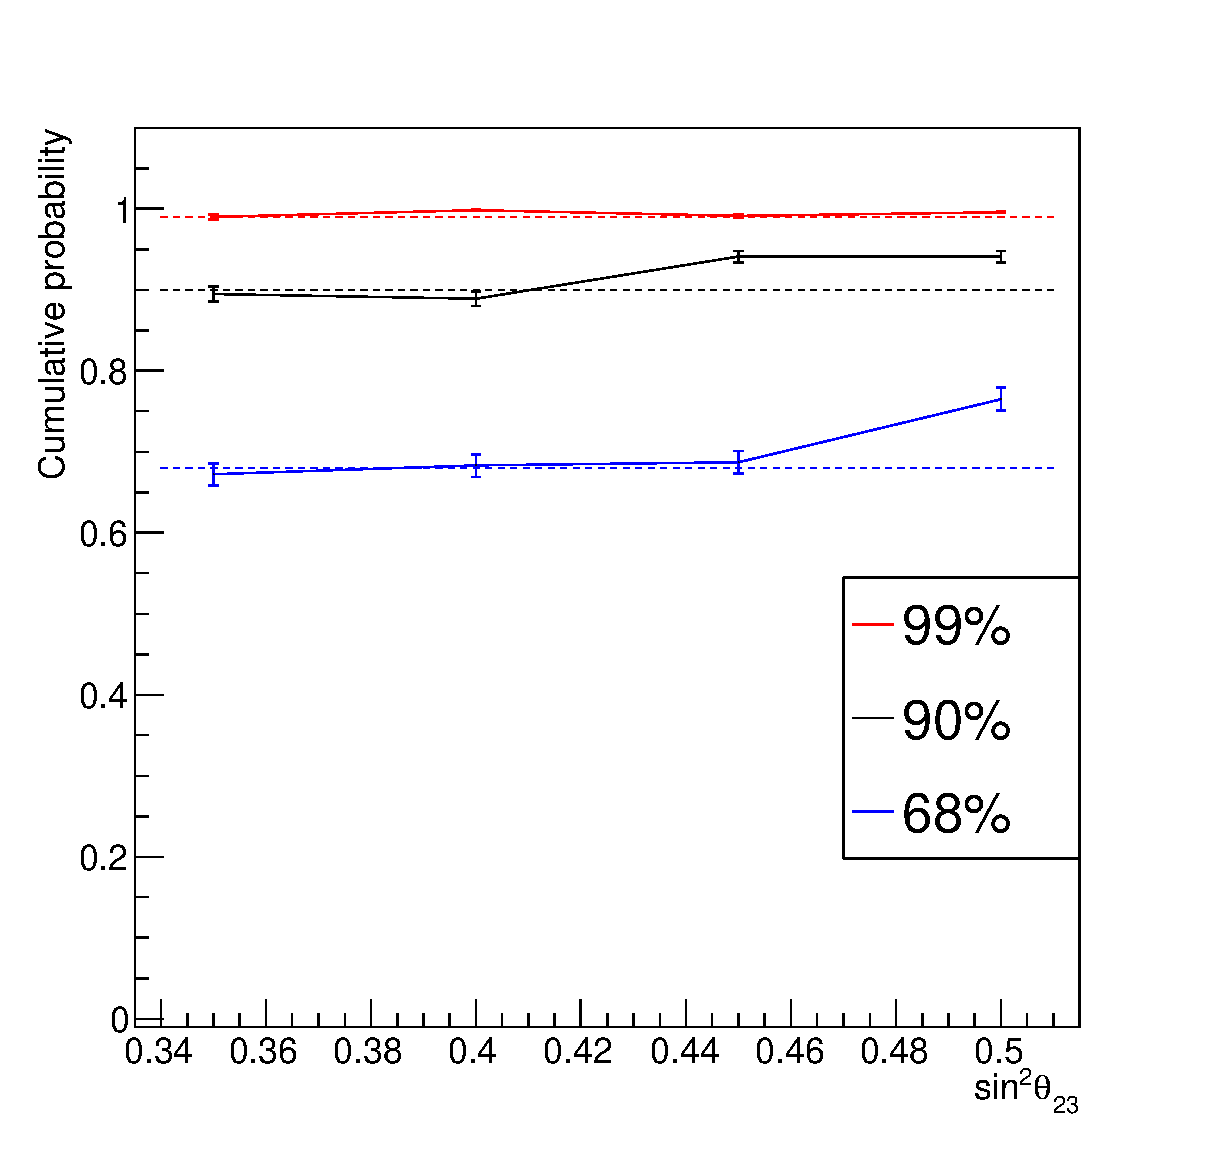
\includegraphics[width=14pc]{./images/appendix/coverage/coverage_study_1D_stats_theta23_new_all.eps}
\caption {
 Summary of figures \ref{fig:prob_1D_theta23_0}-\ref{fig:prob_1D_theta23_3}
showing the value of cumulative probability for $\Delta\chi^{2}=6.63$ (canonical value for 99\%), $\Delta\chi^{2}=2.71$ (canonical value for 90\%) and $\Delta\chi^{2}=1.0$ (canonical value for 68\%) vs the value of $sin^{2}\theta_{23}$.
	}
\label{fig:prob_1D_theta23_all}
\end{minipage}
\end{figure*}
\end{center}


%% FIGURES FOR 1D theta13

\begin{center}
\begin{figure*}[htb]
\begin{minipage}[t]{0.46\linewidth}
\center
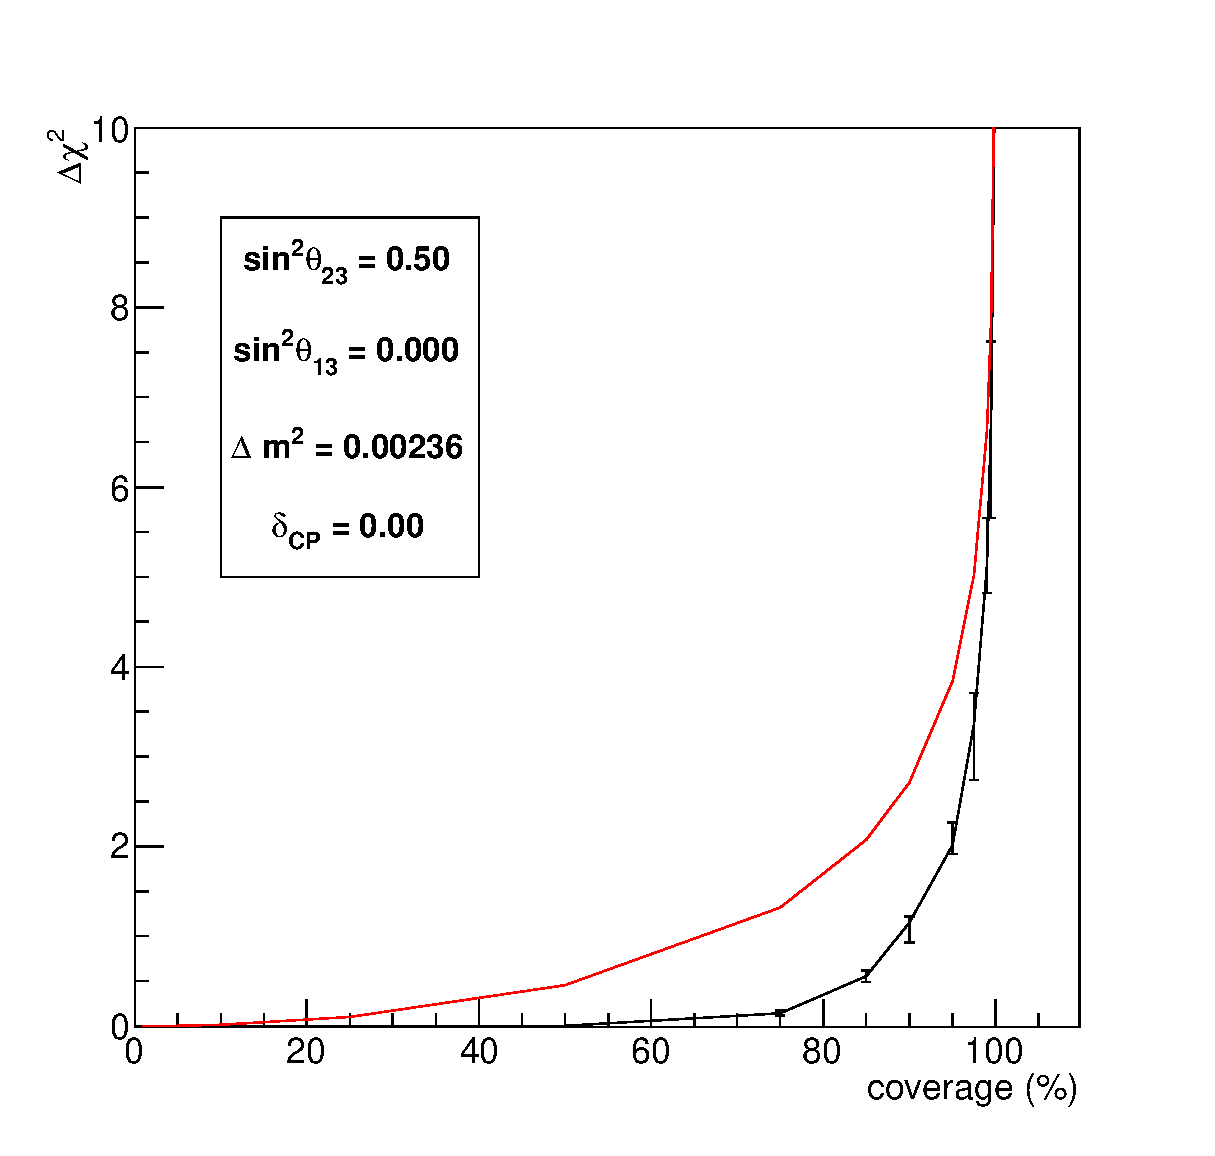
\includegraphics[width=14pc]{./images/appendix/coverage/coverage_study_1D_theta13_0.eps}
\center
\caption {
  Distribution of $\Delta\chi^{2}$ vs coverage in the $sin^{2}\theta_{13}$ parameter space
  from 1k toy MC experiments generated with the Run 1+2+3 POT
  with statistical fluctuations at the oscillation point indicated in the legend.
}
\label{fig:cov_1D_theta13_0}
\end{minipage}
\hspace{0.03\linewidth}
\begin{minipage}[t]{0.46\linewidth}
\center
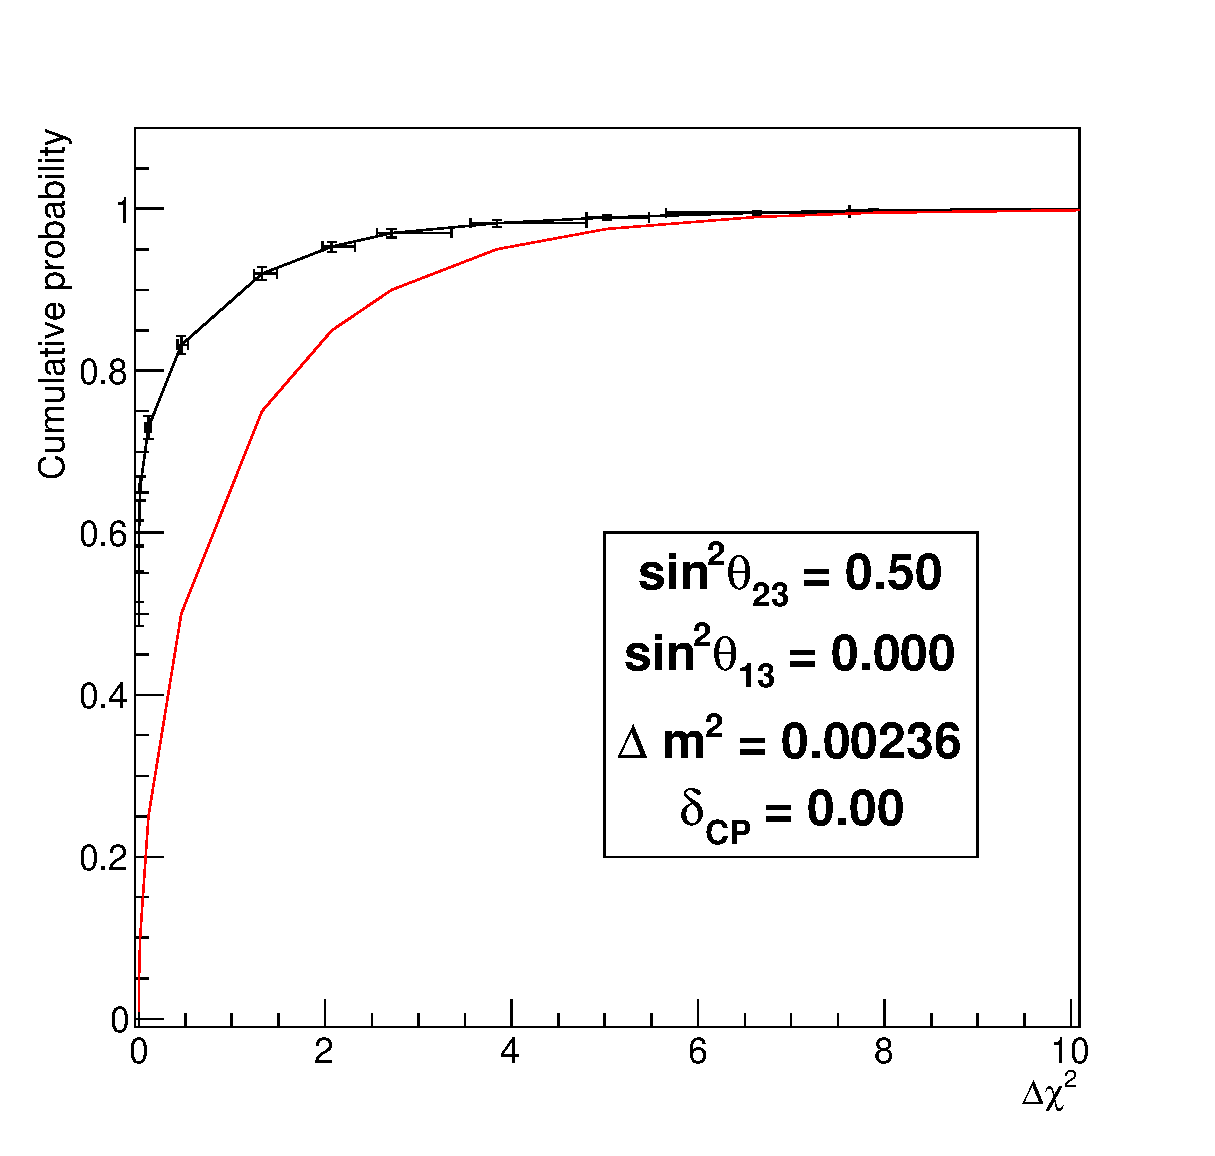
\includegraphics[width=14pc]{./images/appendix/coverage/coverage_study_1D_stats_theta13_new_0.eps}
\center
\caption {
  Distribution of  cumulative probability vs $\Delta\chi^{2}$ in the $sin^{2}\theta_{13}$ parameter space
  from 1k toy MC experiments generated with the Run 1+2+3 POT
  with statistical fluctuations at the oscillation point indicated in the legend.
}
\label{fig:prob_1D_theta13_0}
\end{minipage}
\vfill
\vspace*{0.7cm}
\begin{minipage}[t]{0.46\linewidth}
\center
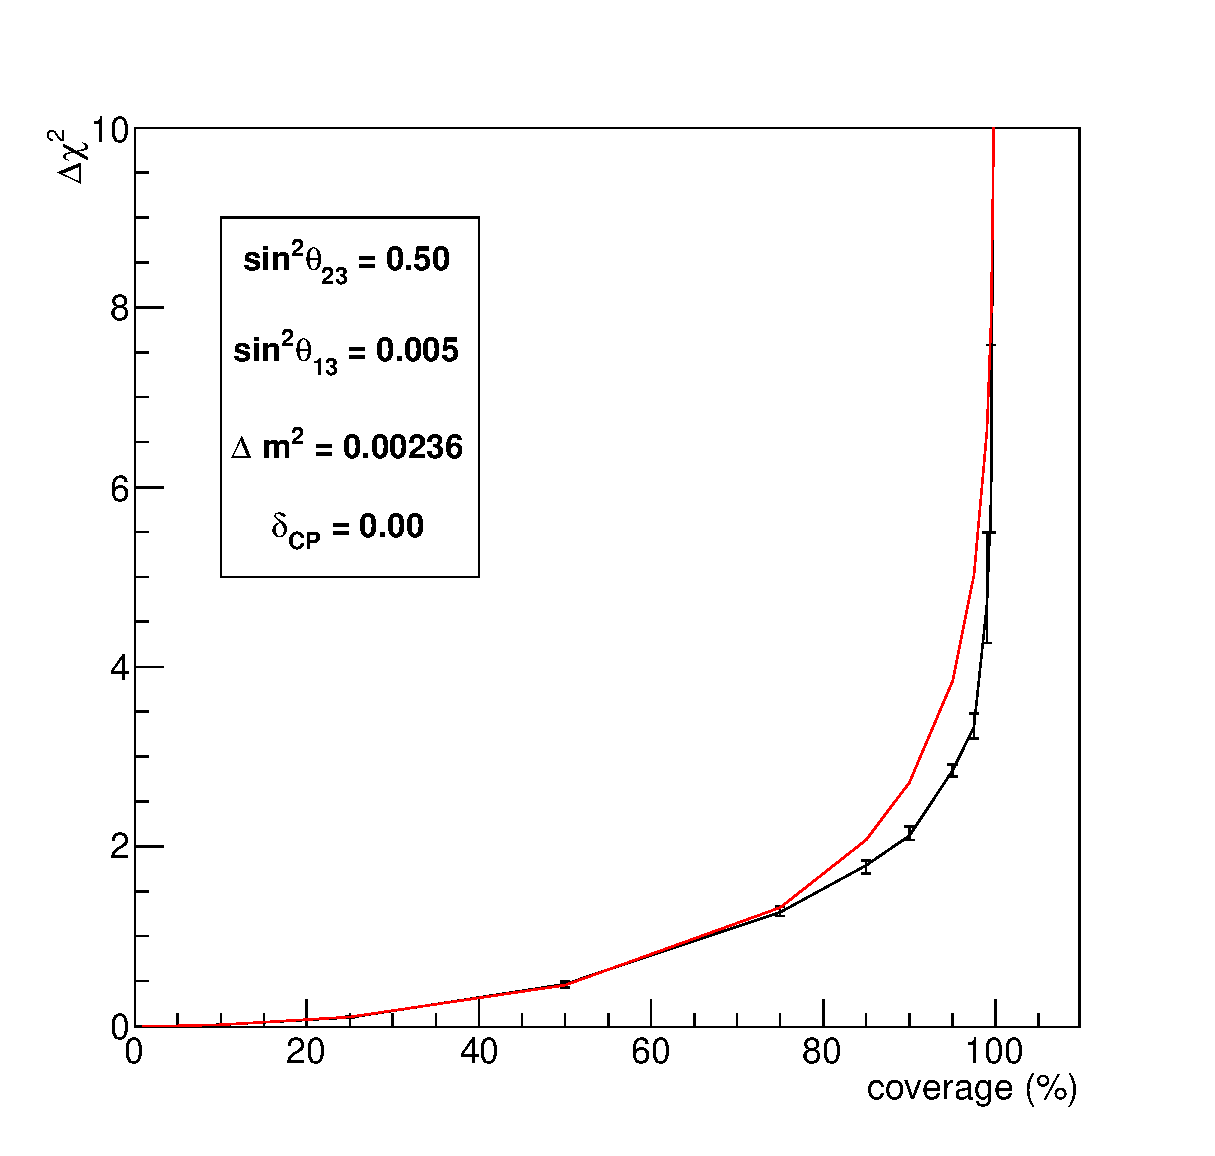
\includegraphics[width=14pc]{./images/appendix/coverage/coverage_study_1D_theta13_1.eps}
\center
\caption {
  Distribution of $\Delta\chi^{2}$ vs coverage in the $sin^{2}\theta_{13}$ parameter space
  from 1k toy MC experiments generated with the Run 1+2+3 POT
  with statistical fluctuations at the oscillation point indicated in the legend.
}
\label{fig:cov_1D_theta13_1}
\end{minipage}
\hspace{0.03\linewidth}
\begin{minipage}[t]{0.46\linewidth}
\center
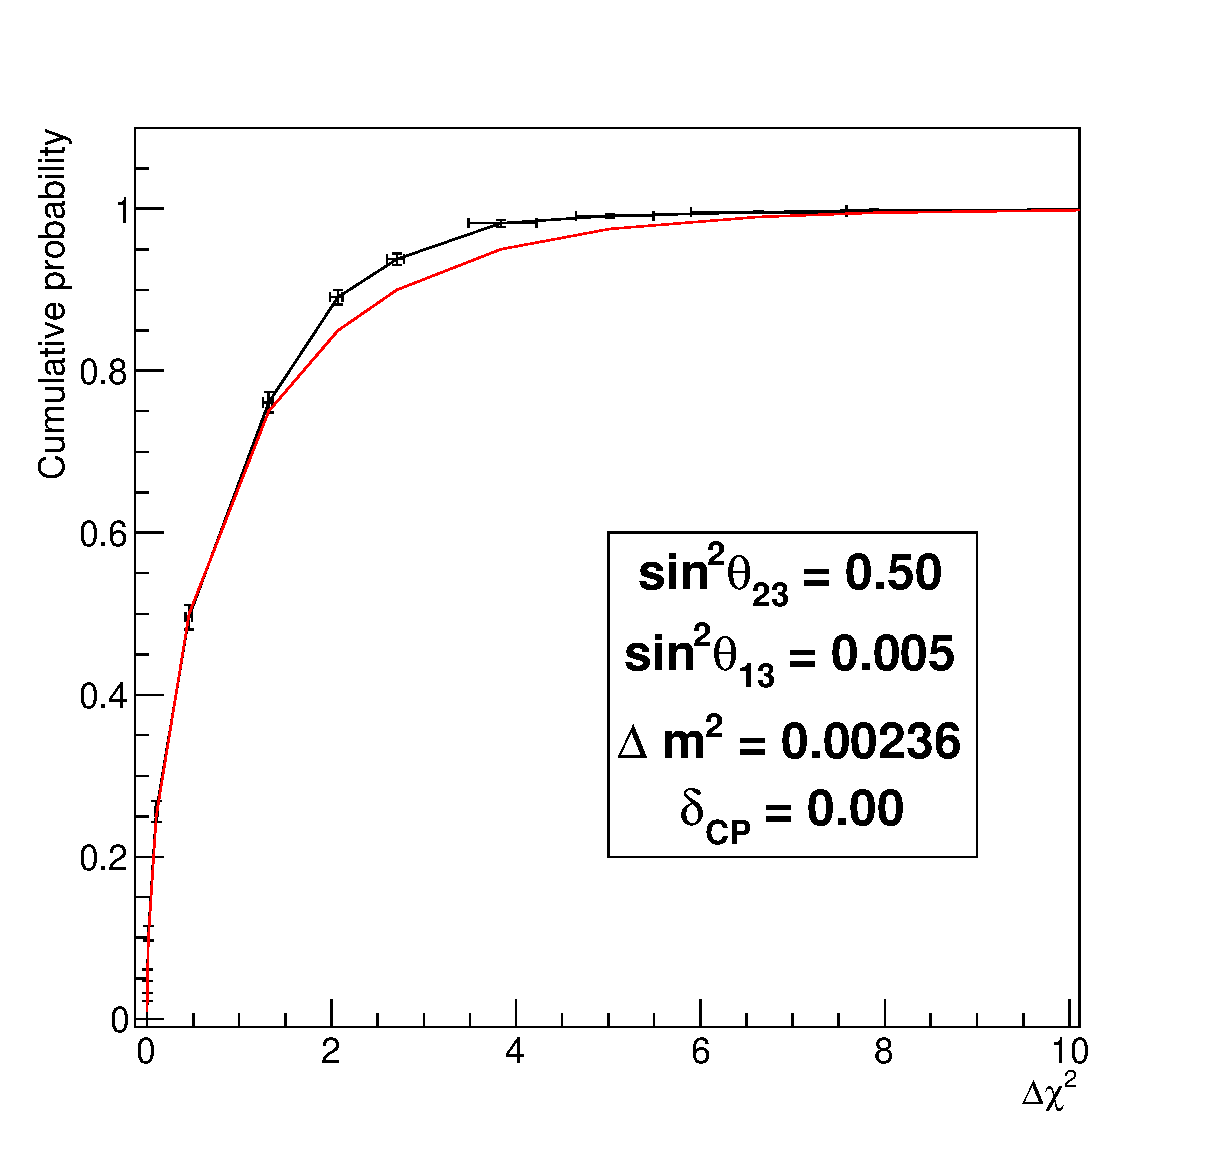
\includegraphics[width=14pc]{./images/appendix/coverage/coverage_study_1D_stats_theta13_new_1.eps}
\center
\caption {
  Distribution of  cumulative probability vs $\Delta\chi^{2}$ in the $sin^{2}\theta_{13}$ parameter space
  from 1k toy MC experiments generated with the Run 1+2+3 POT
  with statistical fluctuations at the oscillation point indicated in the legend.
}
\label{fig:prob_1D_theta13_1}
\end{minipage}
\vfill
\vspace*{0.7cm}
\begin{minipage}[t]{0.46\linewidth}
\center
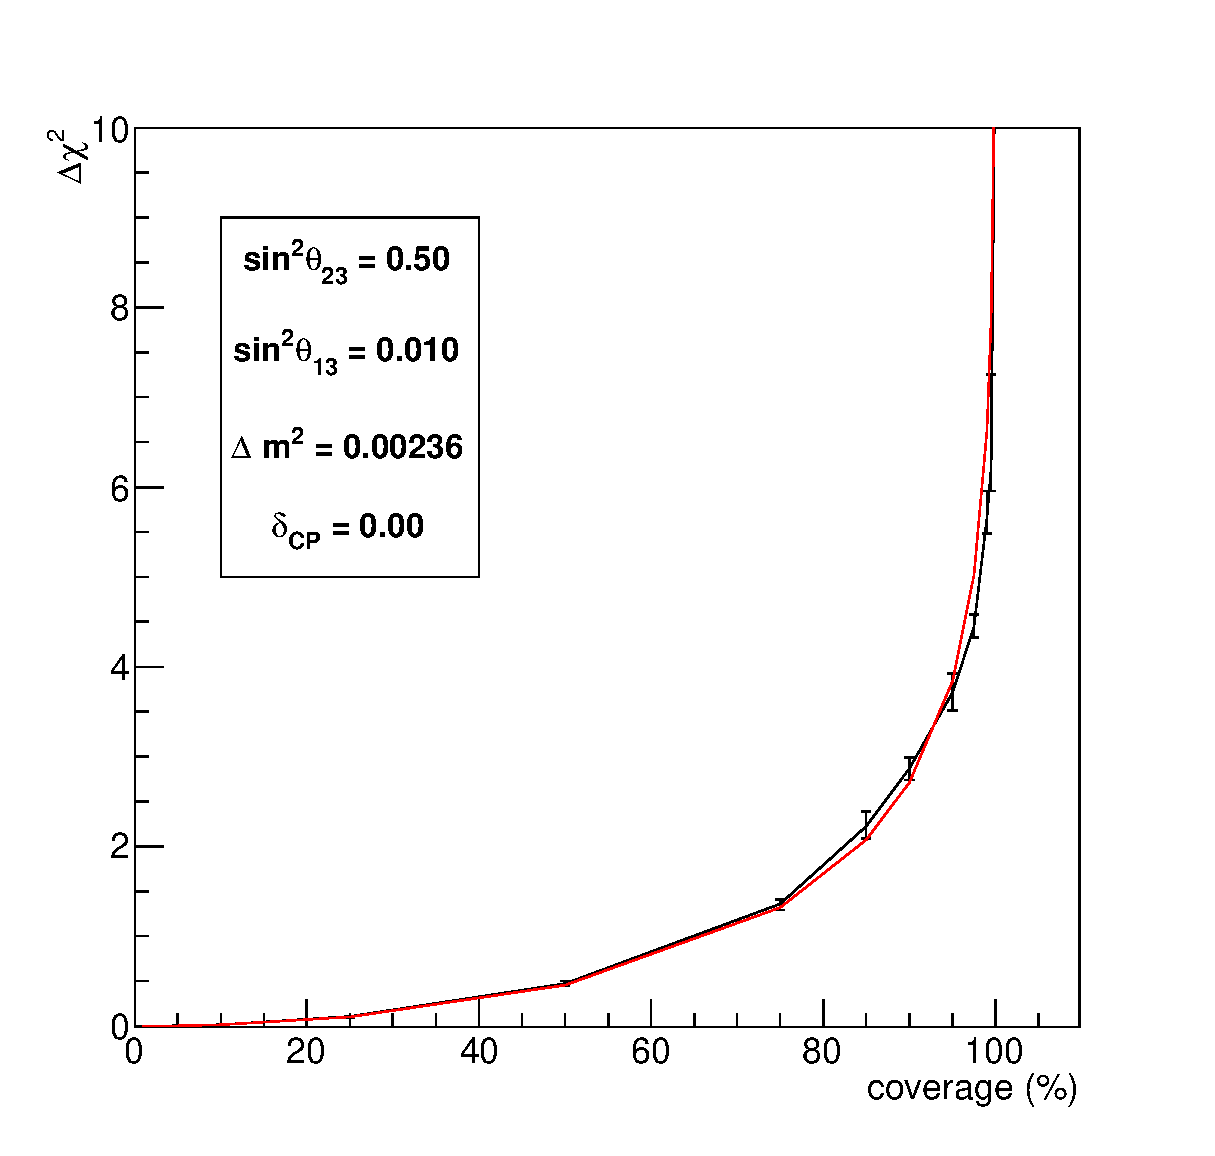
\includegraphics[width=14pc]{./images/appendix/coverage/coverage_study_1D_theta13_2.eps}
\center
\caption {
  Distribution of $\Delta\chi^{2}$ vs coverage in the $sin^{2}\theta_{13}$ parameter space
  from 1k toy MC experiments generated with the Run 1+2+3 POT
  with statistical fluctuations at the oscillation point indicated in the legend.
}
\label{fig:cov_1D_theta13_2}
\end{minipage}
\hspace{0.03\linewidth}
\begin{minipage}[t]{0.46\linewidth}
\center
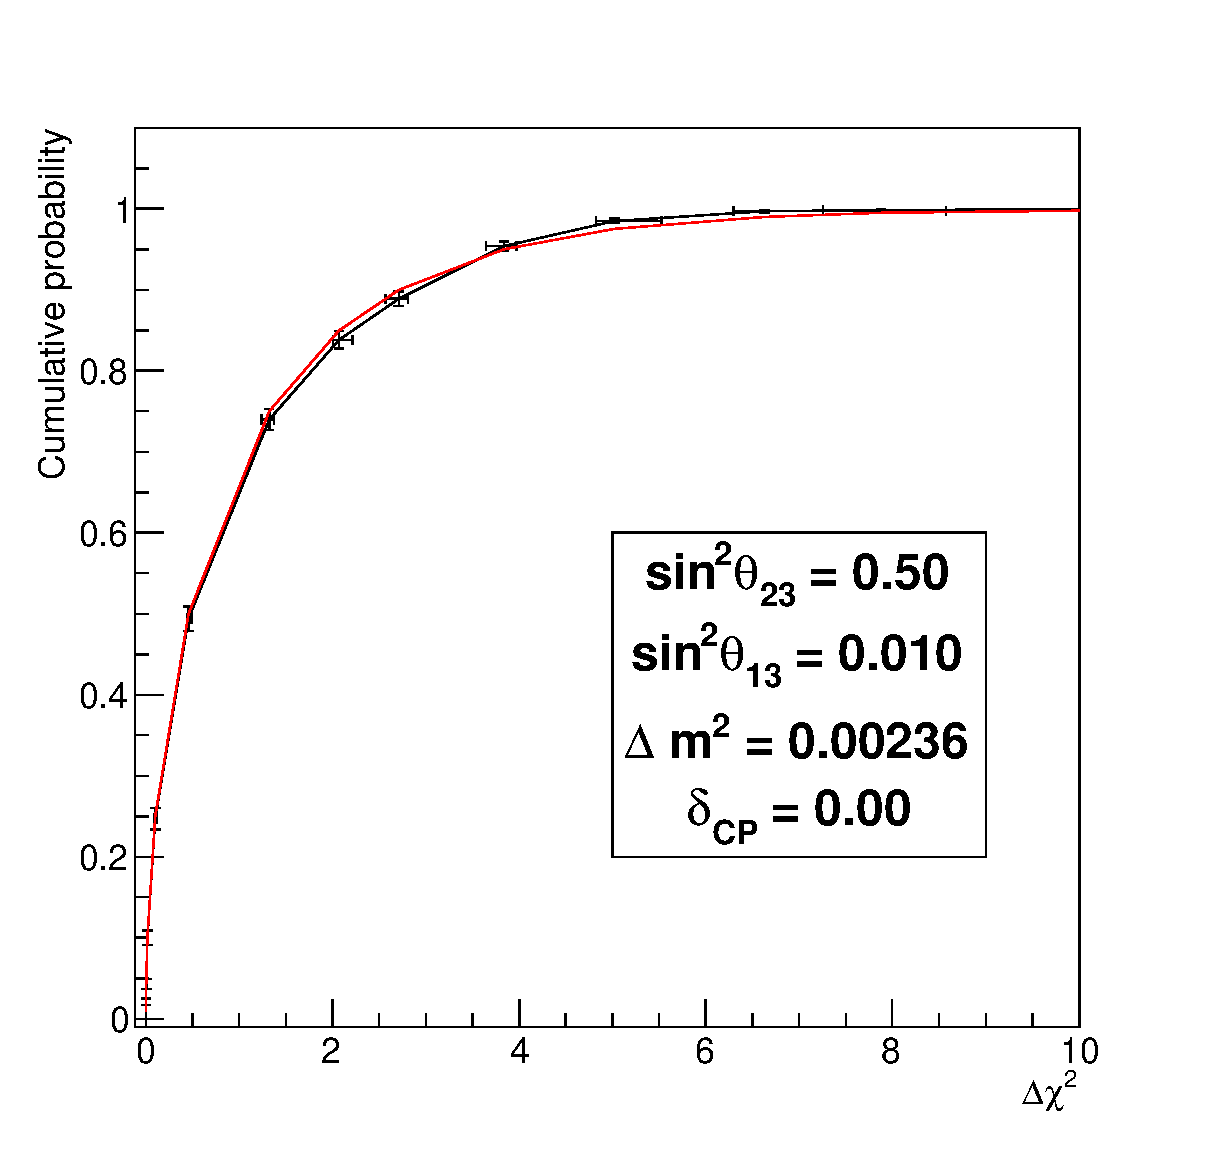
\includegraphics[width=14pc]{./images/appendix/coverage/coverage_study_1D_stats_theta13_new_2.eps}
\center
\caption {
  Distribution of  cumulative probability vs $\Delta\chi^{2}$ in the $sin^{2}\theta_{13}$ parameter space
  from 1k toy MC experiments generated with the Run 1+2+3 POT
  with statistical fluctuations at the oscillation point indicated in the legend.
}
\label{fig:prob_1D_theta13_2}
\end{minipage}
\end{figure*}
\end{center}
\begin{center}
\begin{figure*}[htb]
\begin{minipage}[t]{0.46\linewidth}
\center
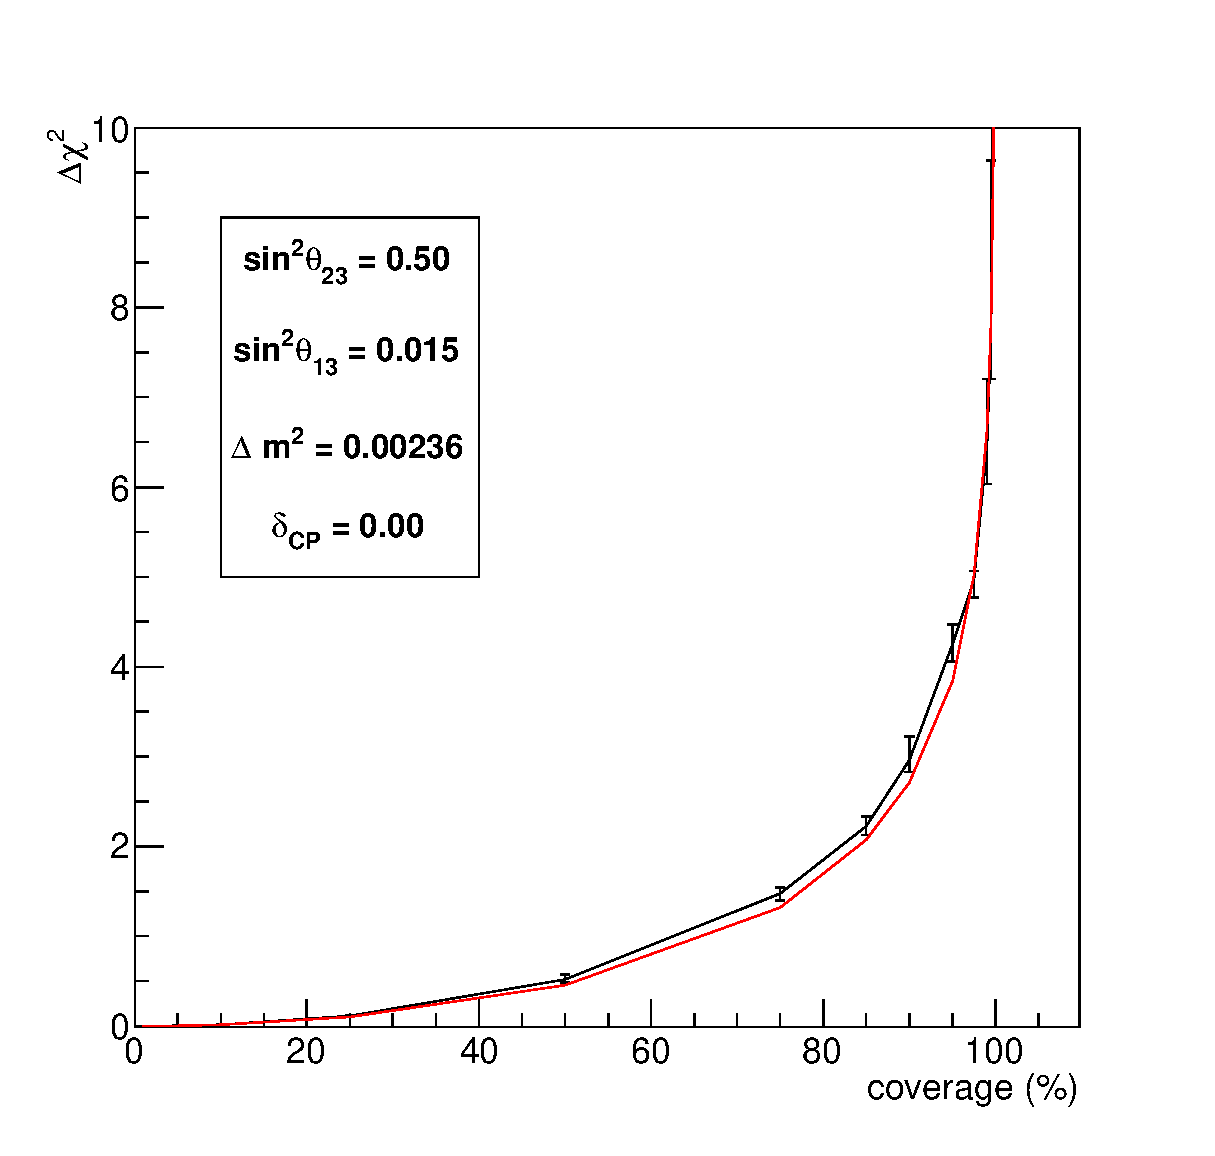
\includegraphics[width=14pc]{./images/appendix/coverage/coverage_study_1D_theta13_3.eps}
\center
\caption {
  Distribution of $\Delta\chi^{2}$ vs coverage in the $sin^{2}\theta_{13}$ parameter space
  from 1k toy MC experiments generated with the Run 1+2+3 POT
  with statistical fluctuations at the oscillation point indicated in the legend.
}
\label{fig:cov_1D_theta13_3}
\end{minipage}
\hspace{0.03\linewidth}
\begin{minipage}[t]{0.46\linewidth}
\center
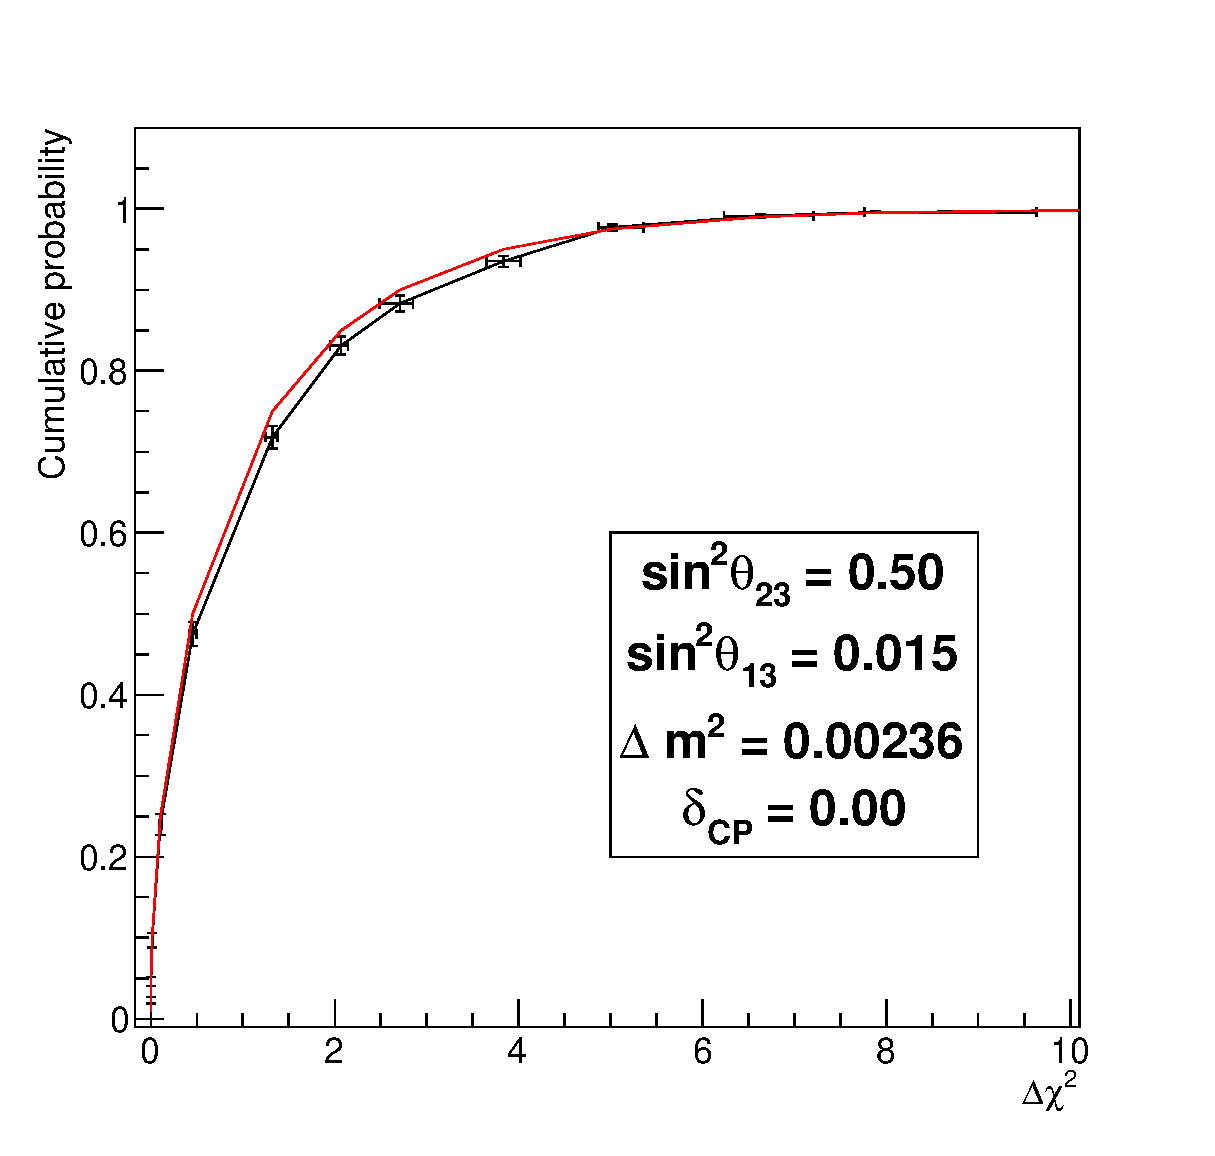
\includegraphics[width=14pc]{./images/appendix/coverage/coverage_study_1D_stats_theta13_new_3.eps}
\center
\caption {
  Distribution of  cumulative probability vs $\Delta\chi^{2}$ in the $sin^{2}\theta_{13}$ parameter space
  from 1k toy MC experiments generated with the Run 1+2+3 POT
  with statistical fluctuations at the oscillation point indicated in the legend.
}
\label{fig:prob_1D_theta13_3}
\end{minipage}
\vfill
\vspace*{0.7cm}
\begin{minipage}[t]{0.46\linewidth}
\center
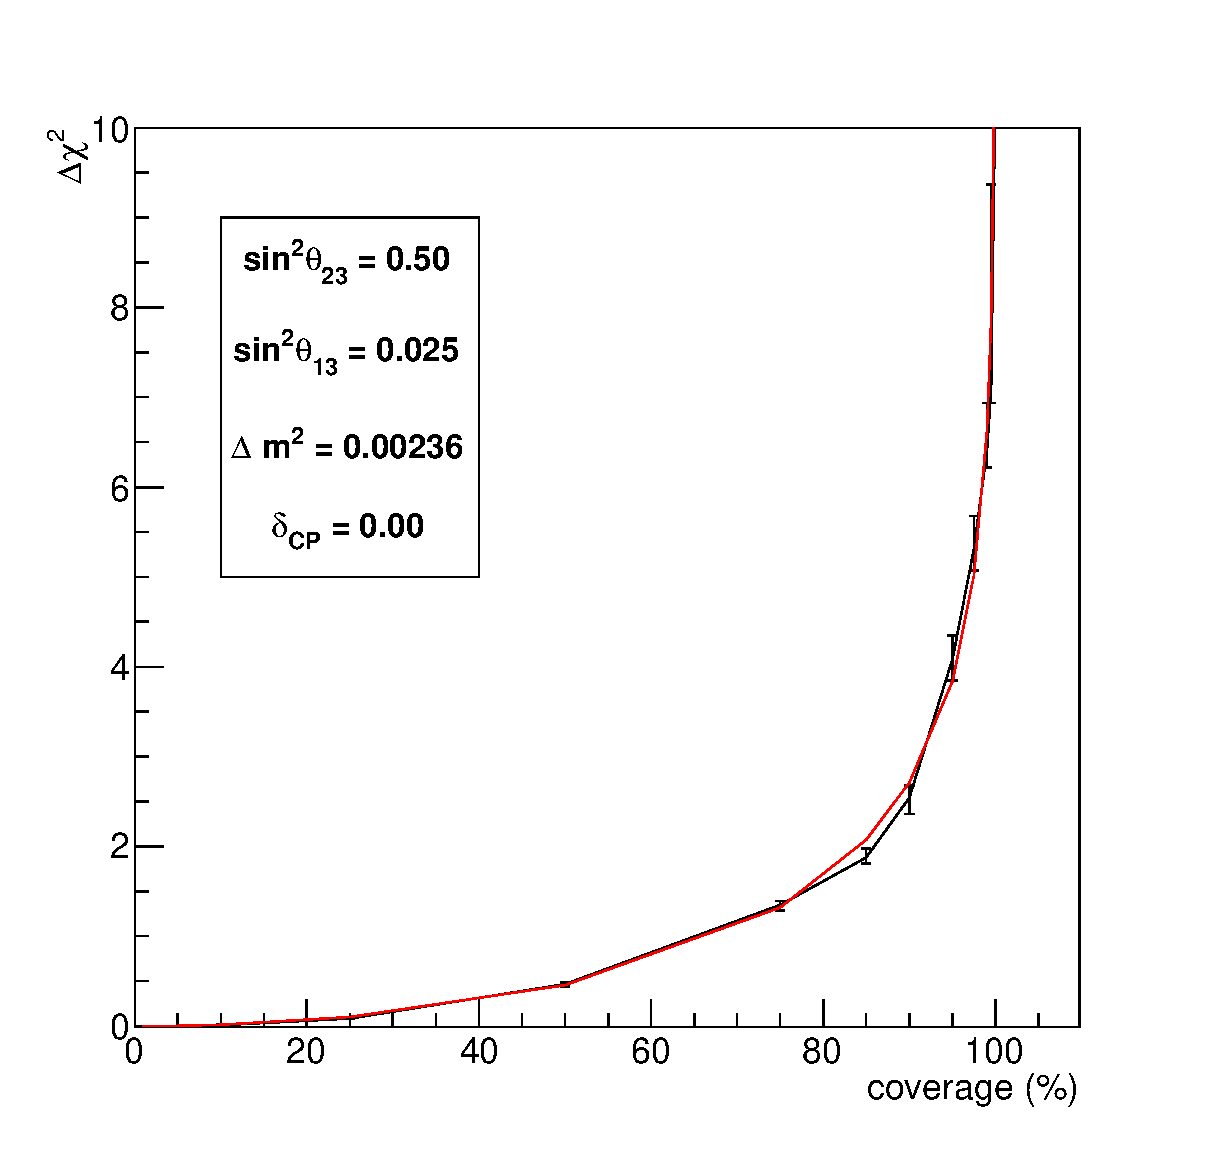
\includegraphics[width=14pc]{./images/appendix/coverage/coverage_study_1D_theta13_4.eps}
\center
\caption {
  Distribution of $\Delta\chi^{2}$ vs coverage in the $sin^{2}\theta_{13}$ parameter space
  from 1k toy MC experiments generated with the Run 1+2+3 POT
  with statistical fluctuations at the oscillation point indicated in the legend.
}
\label{fig:cov_1D_theta13_4}
\end{minipage}
\hspace{0.03\linewidth}
\begin{minipage}[t]{0.46\linewidth}
\center
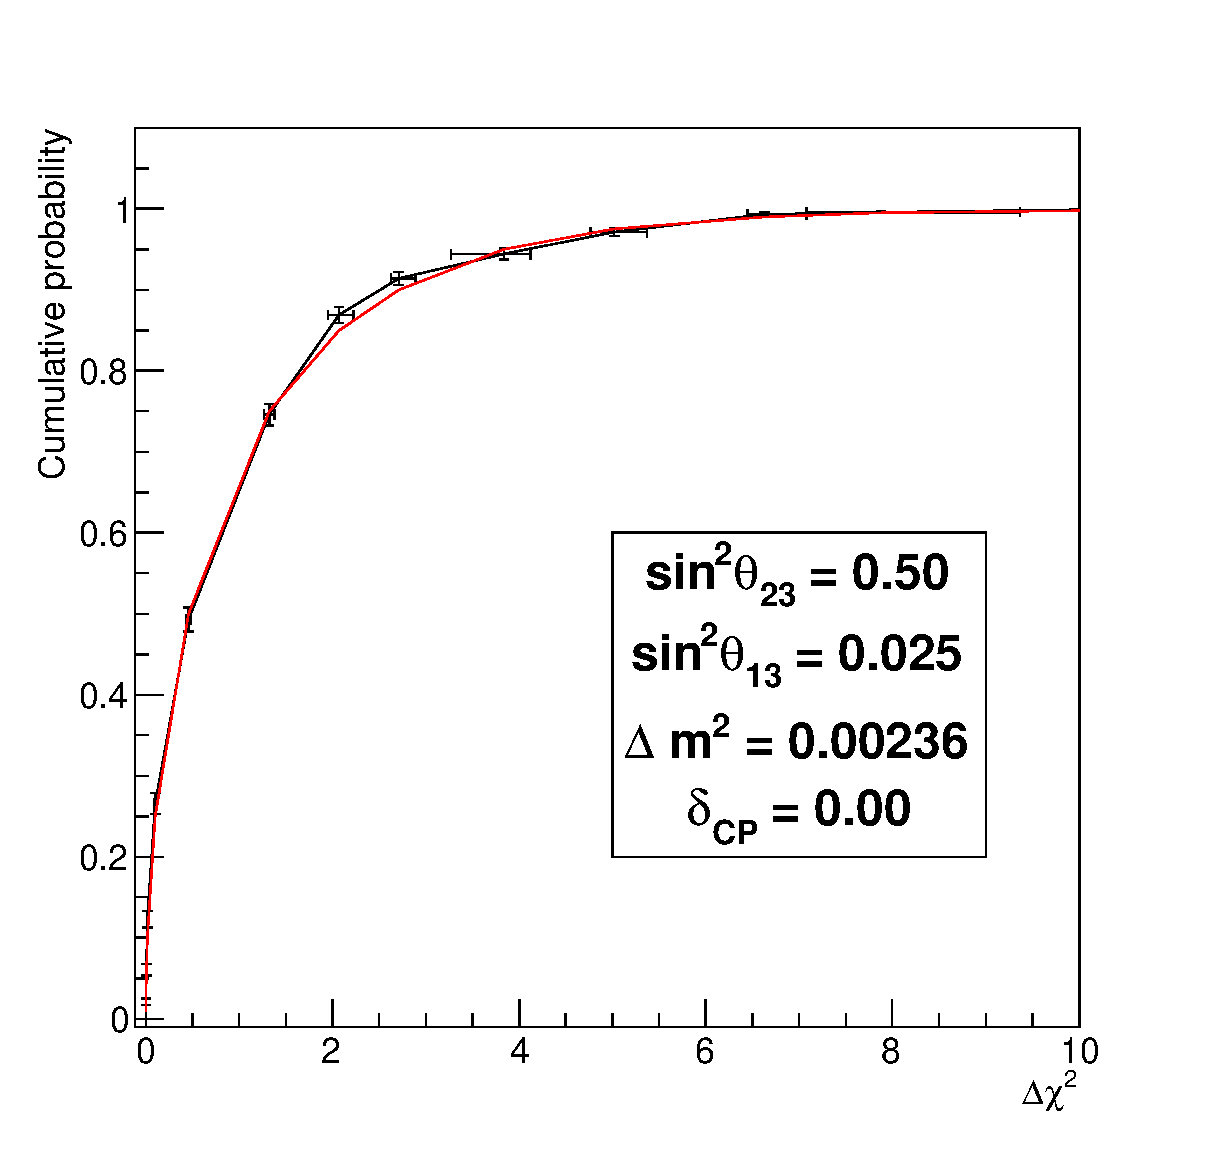
\includegraphics[width=14pc]{./images/appendix/coverage/coverage_study_1D_stats_theta13_new_4.eps}
\center
\caption {
  Distribution of  cumulative probability vs $\Delta\chi^{2}$ in the $sin^{2}\theta_{13}$ parameter space
  from 1k toy MC experiments generated with the Run 1+2+3 POT
  with statistical fluctuations at the oscillation point indicated in the legend.
}
\label{fig:prob_1D_theta13_4}
\end{minipage}
\vfill
\vspace*{0.7cm}
\begin{minipage}[t]{0.46\linewidth}
\center
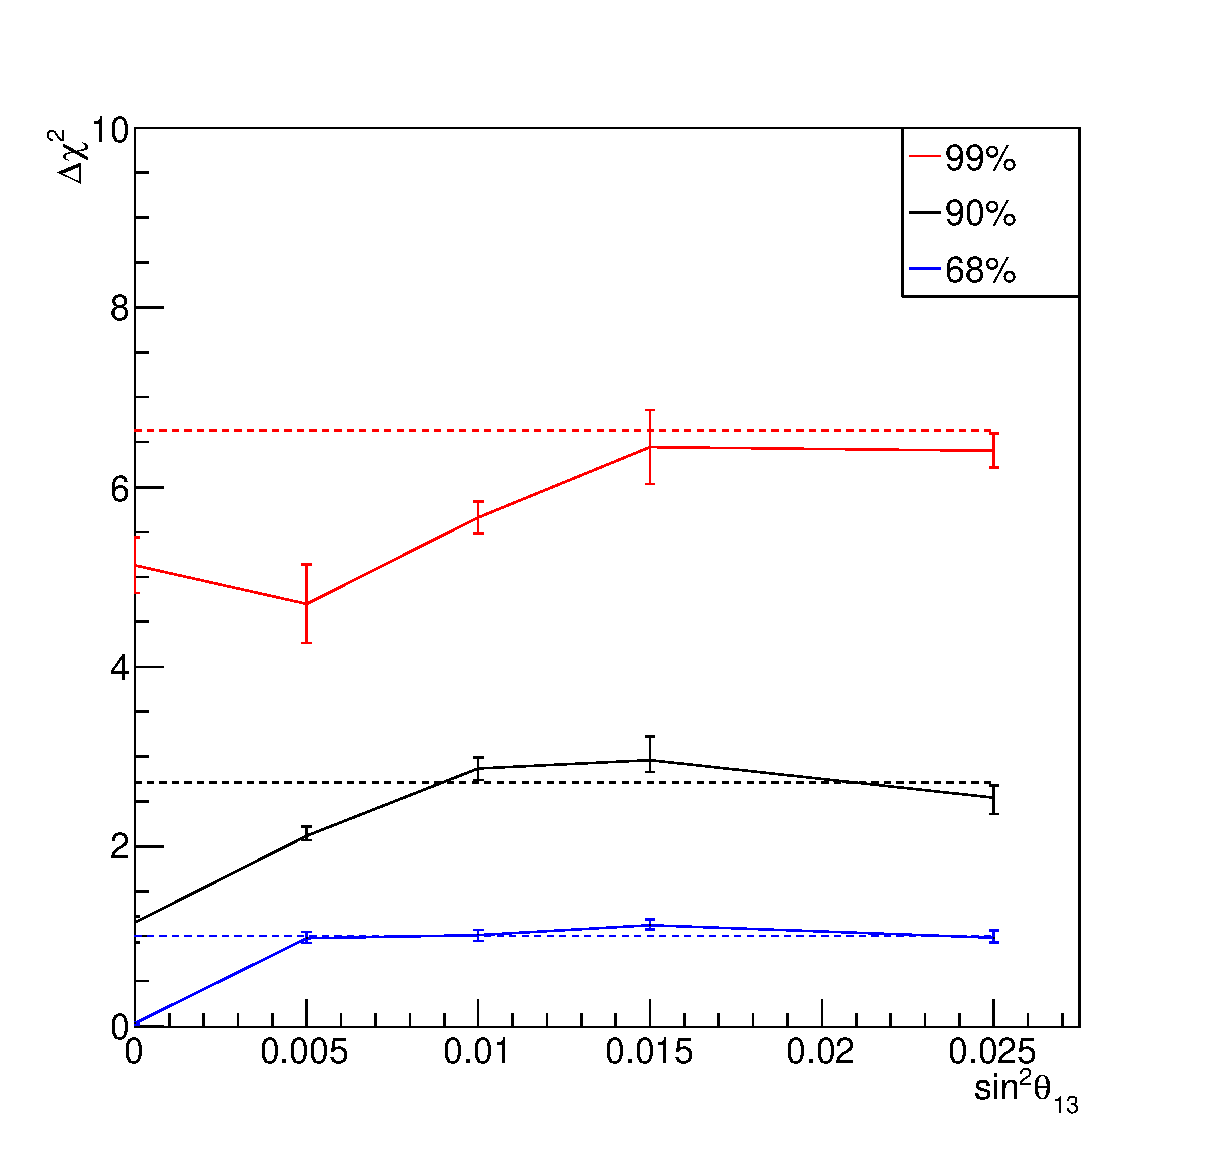
\includegraphics[width=14pc]{./images/appendix/coverage/coverage_study_1D_theta13_all.eps}
\caption {
   Summary of figures \ref{fig:cov_1D_theta13_0}-\ref{fig:cov_1D_theta13_4}
showing the value of $\Delta\chi^{2}$ at 99\%, 90\% and 68\% confidence intervals vs the value of $sin^{2}\theta_{13}$.
Horizontal dashed lines show the canonical $\Delta\chi^{2}$ value for 1 degree of freedom.
	}
\label{fig:cov_1D_theta13_all}
\end{minipage}
\hspace{0.03\linewidth}
\begin{minipage}[t]{0.46\linewidth}
\center
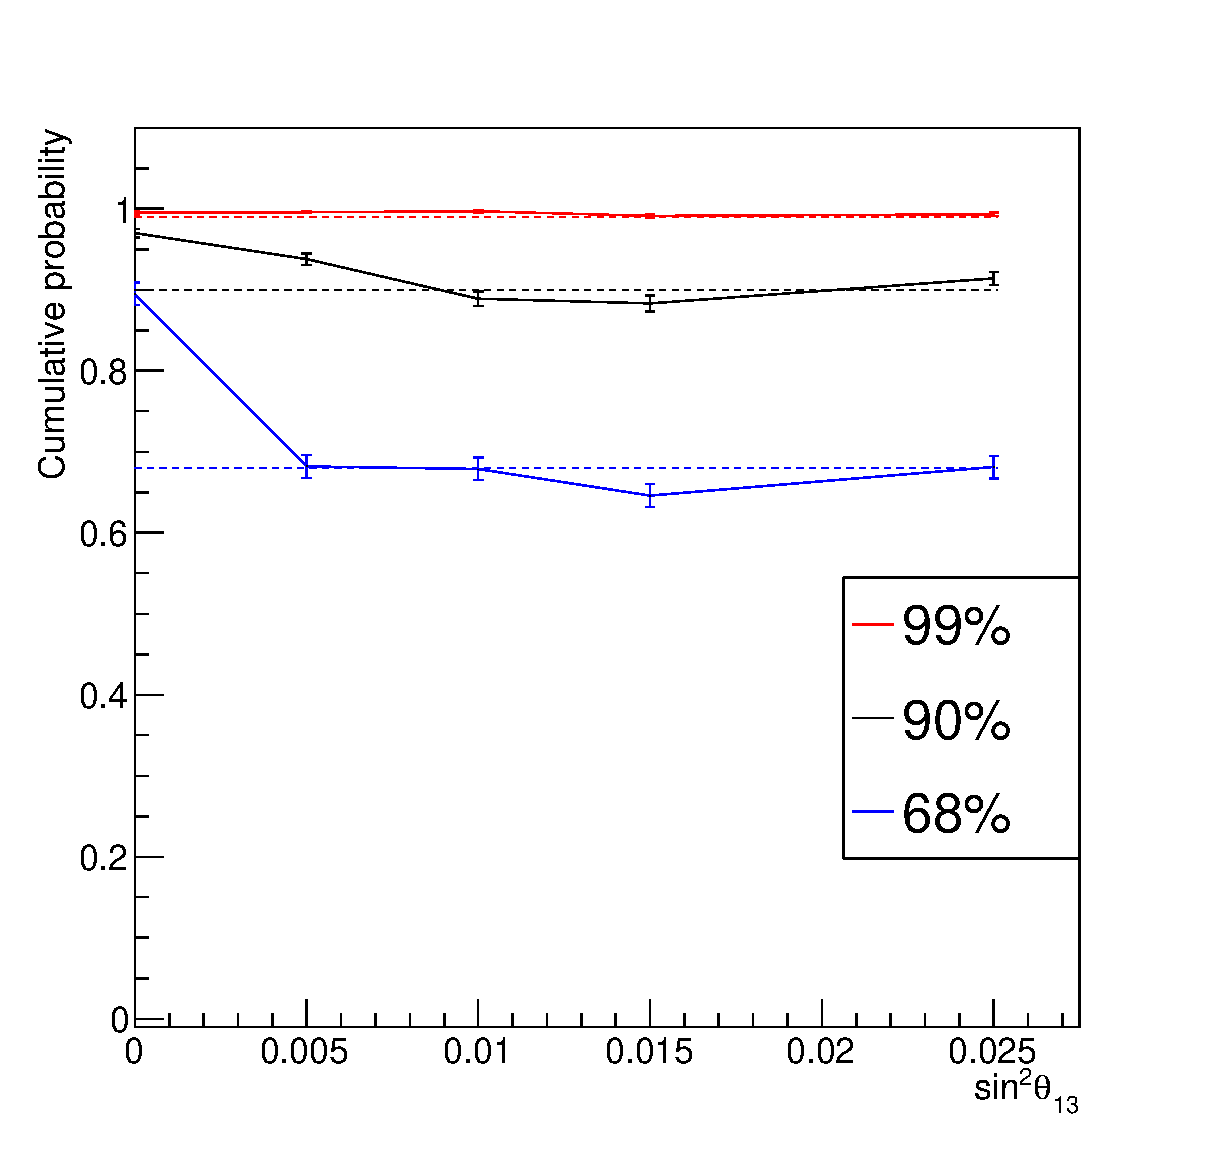
\includegraphics[width=14pc]{./images/appendix/coverage/coverage_study_1D_stats_theta13_new_all.eps}
\caption {
Summary of figures \ref{fig:prob_1D_theta13_0}-\ref{fig:prob_1D_theta13_4}
showing the value of cumulative probability for $\Delta\chi^{2}=6.63$ (canonical value for 99\%), $\Delta\chi^{2}=2.71$ (canonical value for 90\%) and $\Delta\chi^{2}=1.0$ (canonical value for 68\%) vs the value of $sin^{2}\theta_{13}$.
 }
\label{fig:prob_1D_theta13_all}
\end{minipage}
\end{figure*}
\end{center}


%% FIGURES FOR 1D deltacp

\begin{center}
\begin{figure*}[htb]
\begin{minipage}[t]{0.46\linewidth}
\center
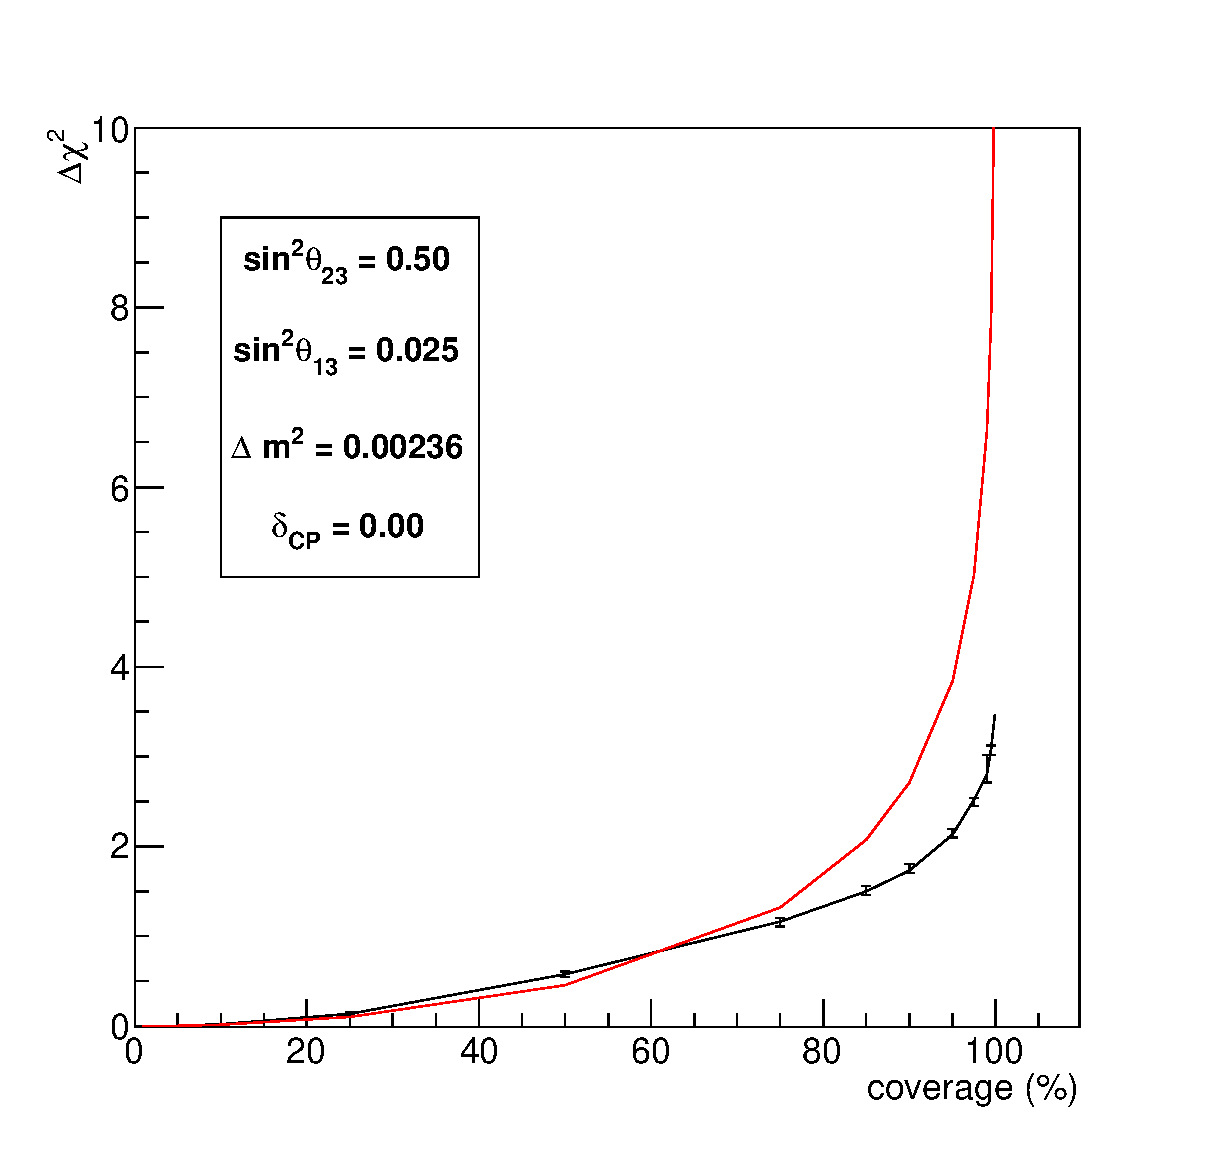
\includegraphics[width=14pc]{./images/appendix/coverage/coverage_study_1D_deltacp_0.eps}
\center
\caption {
  Distribution of $\Delta\chi^{2}$ vs coverage in the $\delta_{CP}$ parameter space
  from 1k toy MC experiments generated with the Run 1+2+3 POT
  with statistical fluctuations at the oscillation point indicated in the legend.
}
\label{fig:cov_1D_deltacp_0}
\end{minipage}
\hspace{0.03\linewidth}
\begin{minipage}[t]{0.46\linewidth}
\center
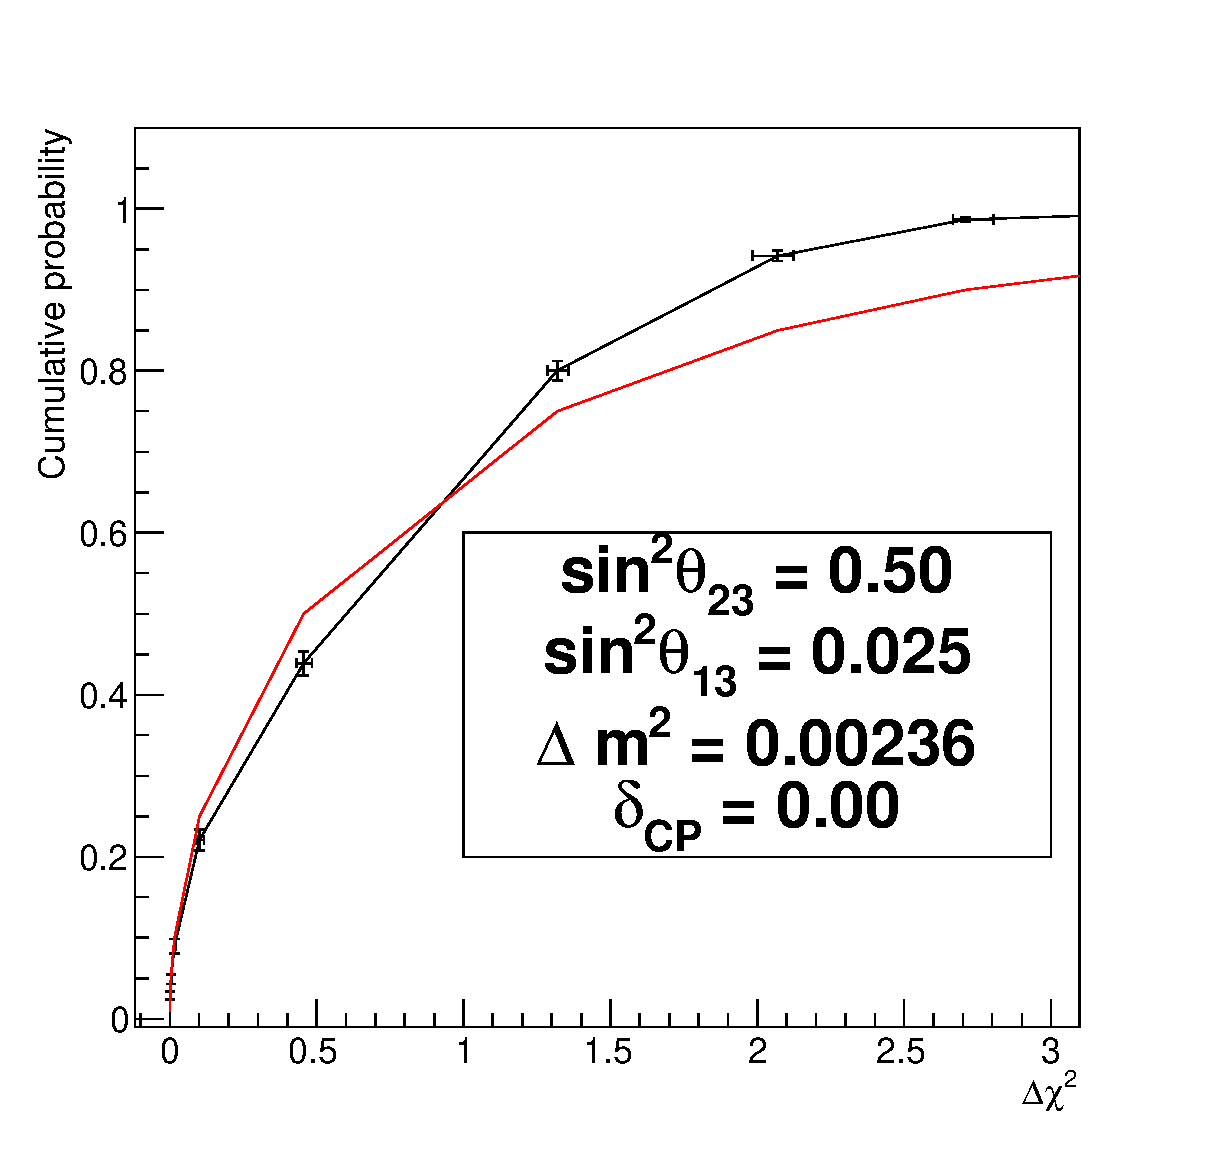
\includegraphics[width=14pc]{./images/appendix/coverage/coverage_study_1D_stats_deltacp_new_0.eps}
\center
\caption {
  Distribution of cumulative probability vs $\Delta\chi^{2}$ in the $\delta_{CP}$ parameter space
  from 1k toy MC experiments generated with the Run 1+2+3 POT
  with statistical fluctuations at the oscillation point indicated in the legend.
}
\label{fig:prob_1D_deltacp_0}
\end{minipage}
\vfill
\vspace*{0.7cm}
\begin{minipage}[t]{0.46\linewidth}
\center
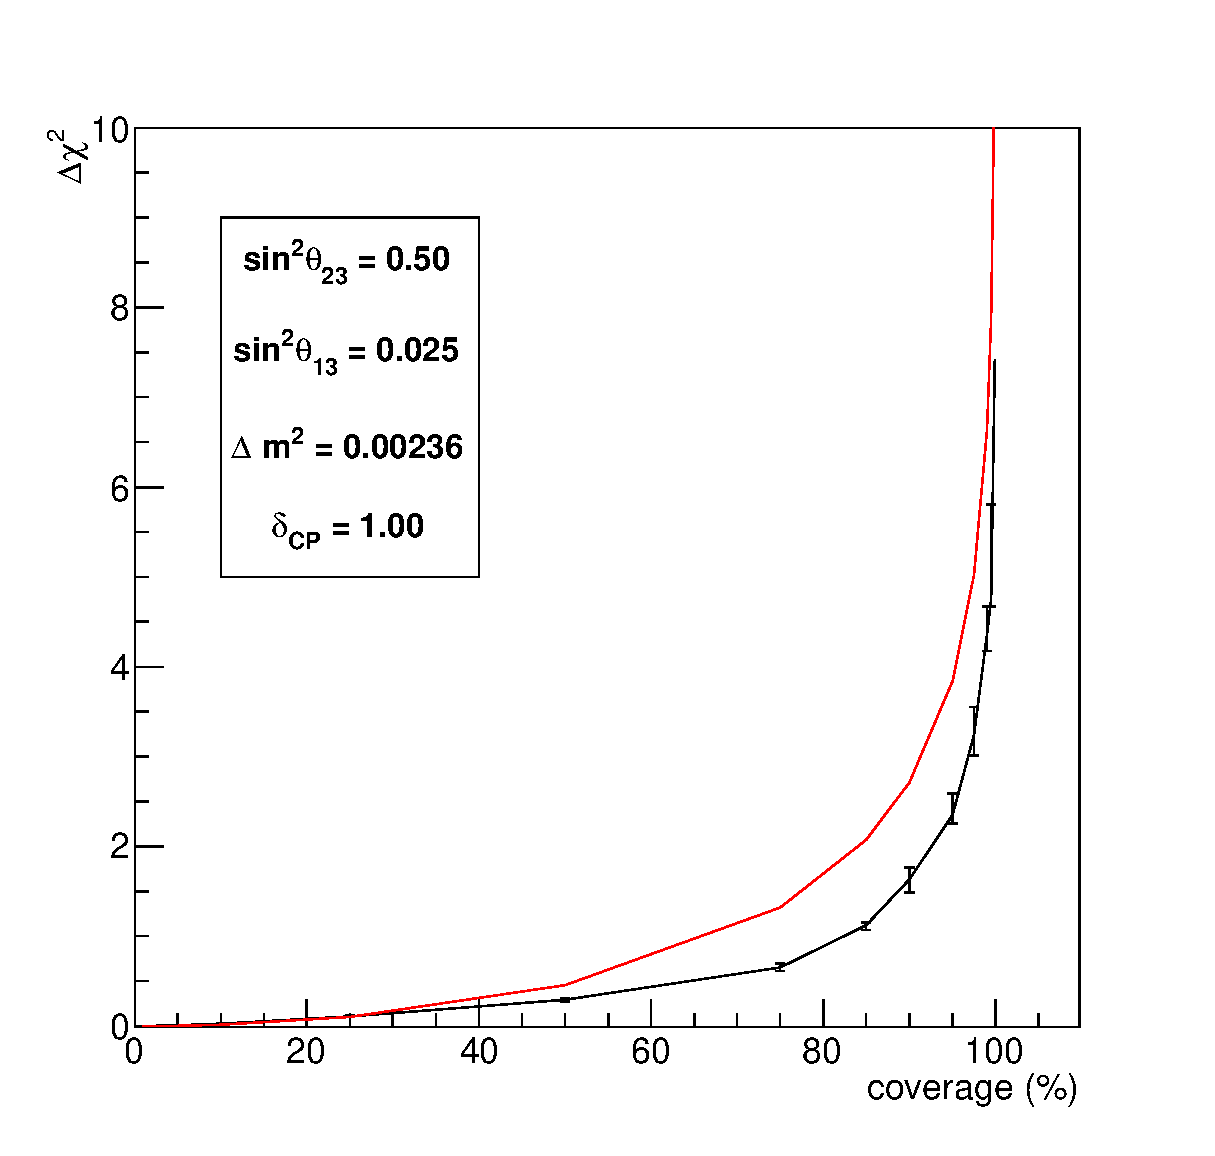
\includegraphics[width=14pc]{./images/appendix/coverage/coverage_study_1D_deltacp_1.eps}
\center
\caption {
  Distribution of $\Delta\chi^{2}$ vs coverage in the $\delta_{CP}$ parameter space
  from 1k toy MC experiments generated with the Run 1+2+3 POT
  with statistical fluctuations at the oscillation point indicated in the legend.
}
\label{fig:cov_1D_deltacp_1}
\end{minipage}
\hspace{0.03\linewidth}
\begin{minipage}[t]{0.46\linewidth}
\center
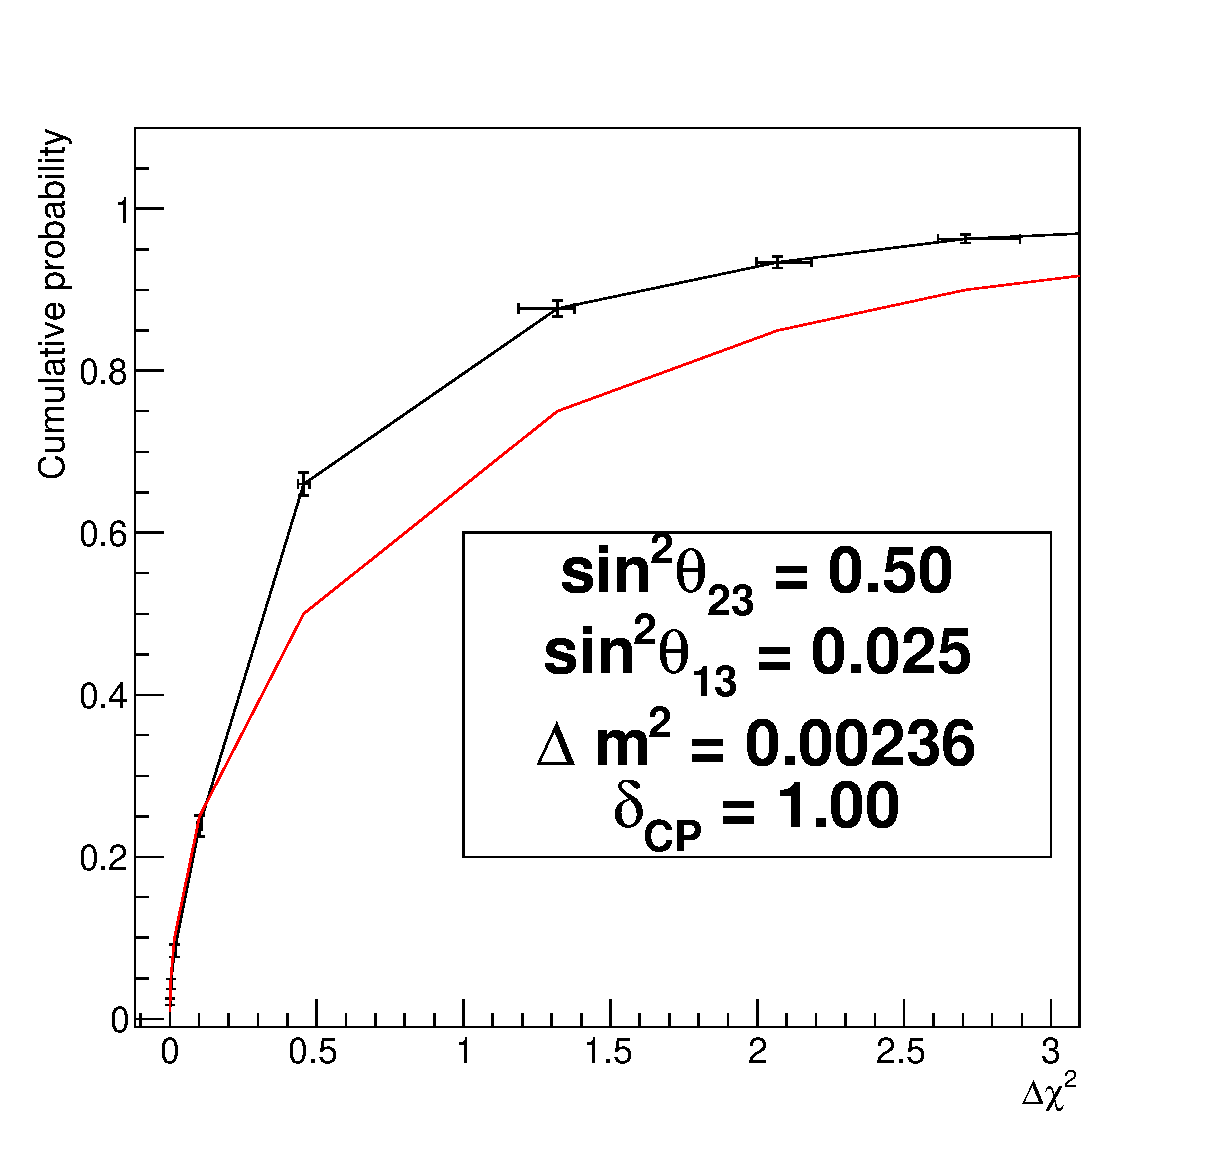
\includegraphics[width=14pc]{./images/appendix/coverage/coverage_study_1D_stats_deltacp_new_1.eps}
\center
\caption {
  Distribution of cumulative probability vs $\Delta\chi^{2}$ in the $\delta_{CP}$ parameter space
  from 1k toy MC experiments generated with the Run 1+2+3 POT
  with statistical fluctuations at the oscillation point indicated in the legend.
}
\label{fig:prob_1D_deltacp_1}
\end{minipage}
\vfill
\vspace*{0.7cm}
\begin{minipage}[t]{0.46\linewidth}
\center
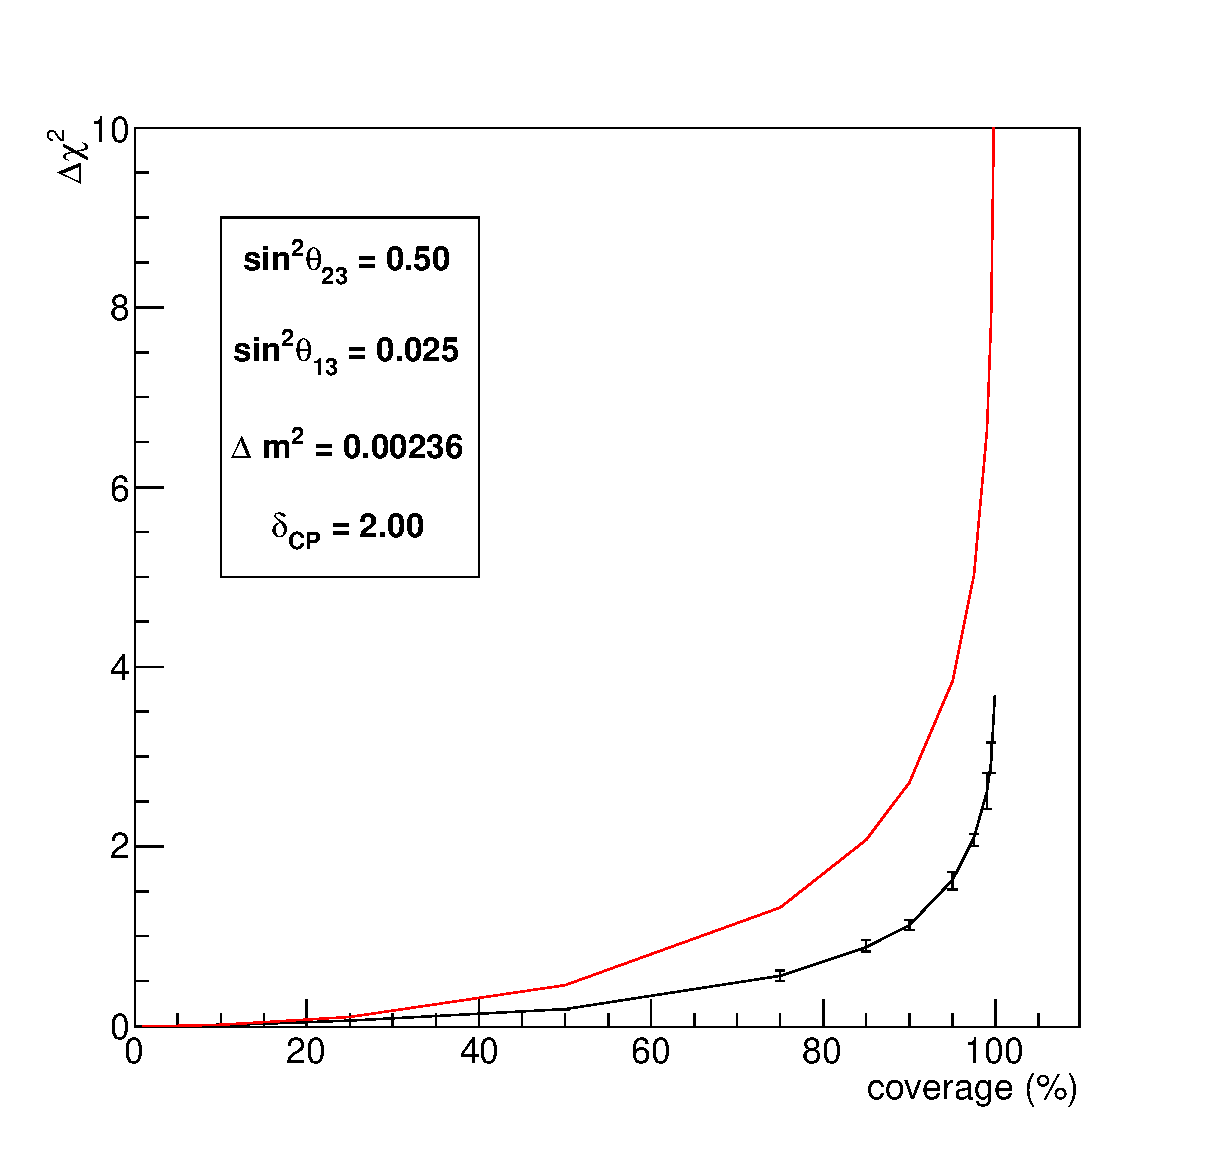
\includegraphics[width=14pc]{./images/appendix/coverage/coverage_study_1D_deltacp_2.eps}
\center
\caption {
  Distribution of $\Delta\chi^{2}$ vs coverage in the $\delta_{CP}$ parameter space
  from 1k toy MC experiments generated with the Run 1+2+3 POT
  with statistical fluctuations at the oscillation point indicated in the legend.
}
\label{fig:cov_1D_deltacp_2}
\end{minipage}
\hspace{0.03\linewidth}
\begin{minipage}[t]{0.46\linewidth}
\center
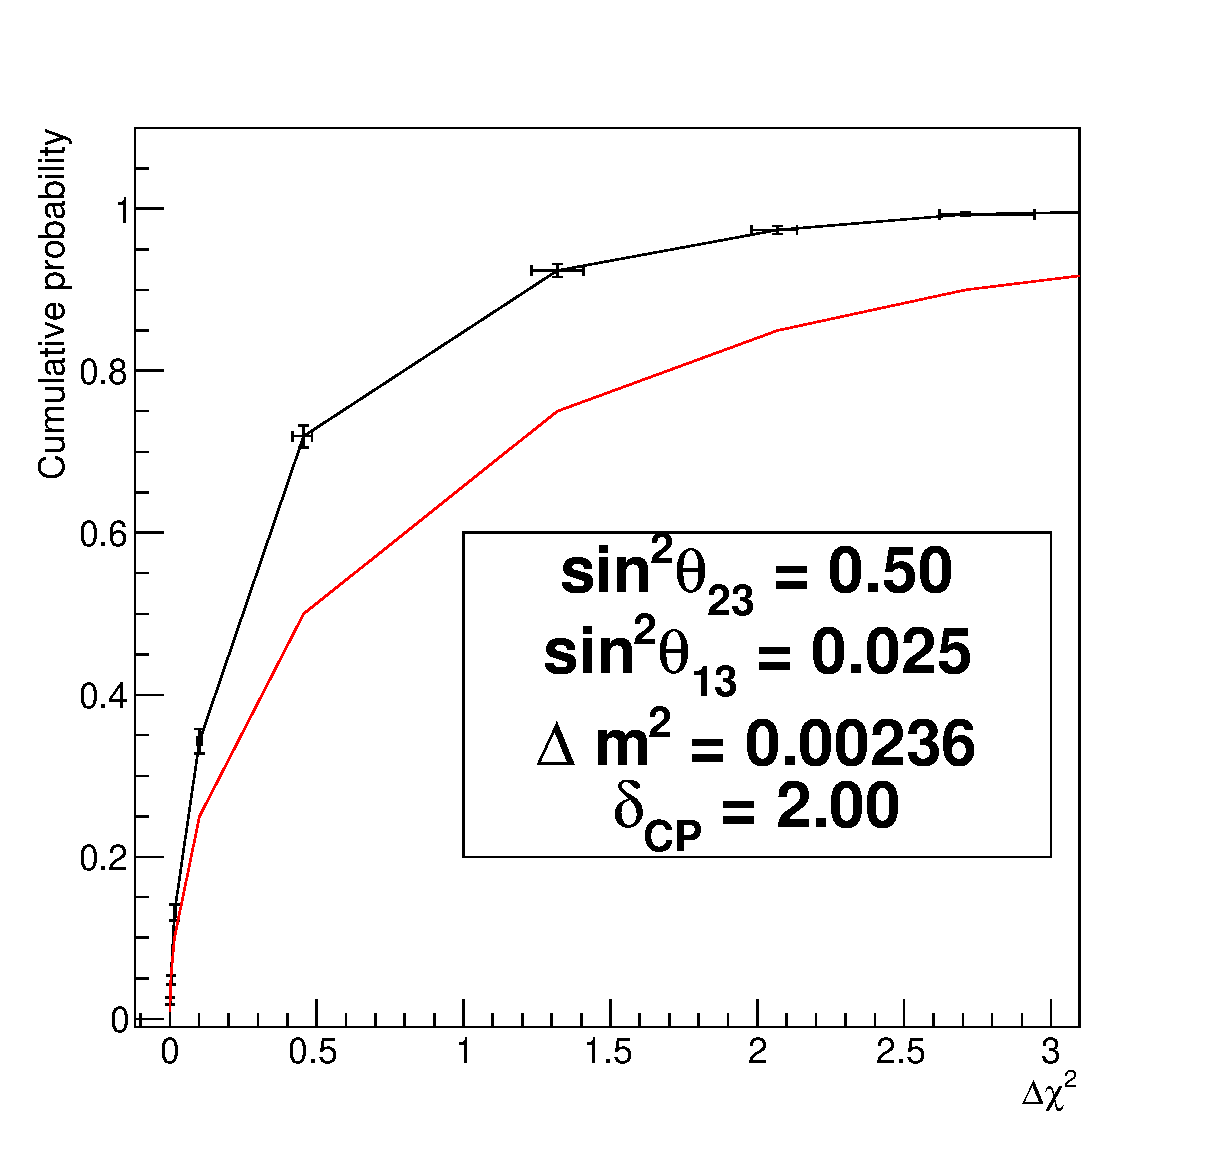
\includegraphics[width=14pc]{./images/appendix/coverage/coverage_study_1D_stats_deltacp_new_2.eps}
\center
\caption {
  Distribution of cumulative probability vs $\Delta\chi^{2}$ in the $\delta_{CP}$ parameter space
  from 1k toy MC experiments generated with the Run 1+2+3 POT
  with statistical fluctuations at the oscillation point indicated in the legend.
}
\label{fig:prob_1D_deltacp_2}
\end{minipage}
\end{figure*}
\end{center}
\begin{center}
\begin{figure*}[htb]
\begin{minipage}[t]{0.46\linewidth}
\center
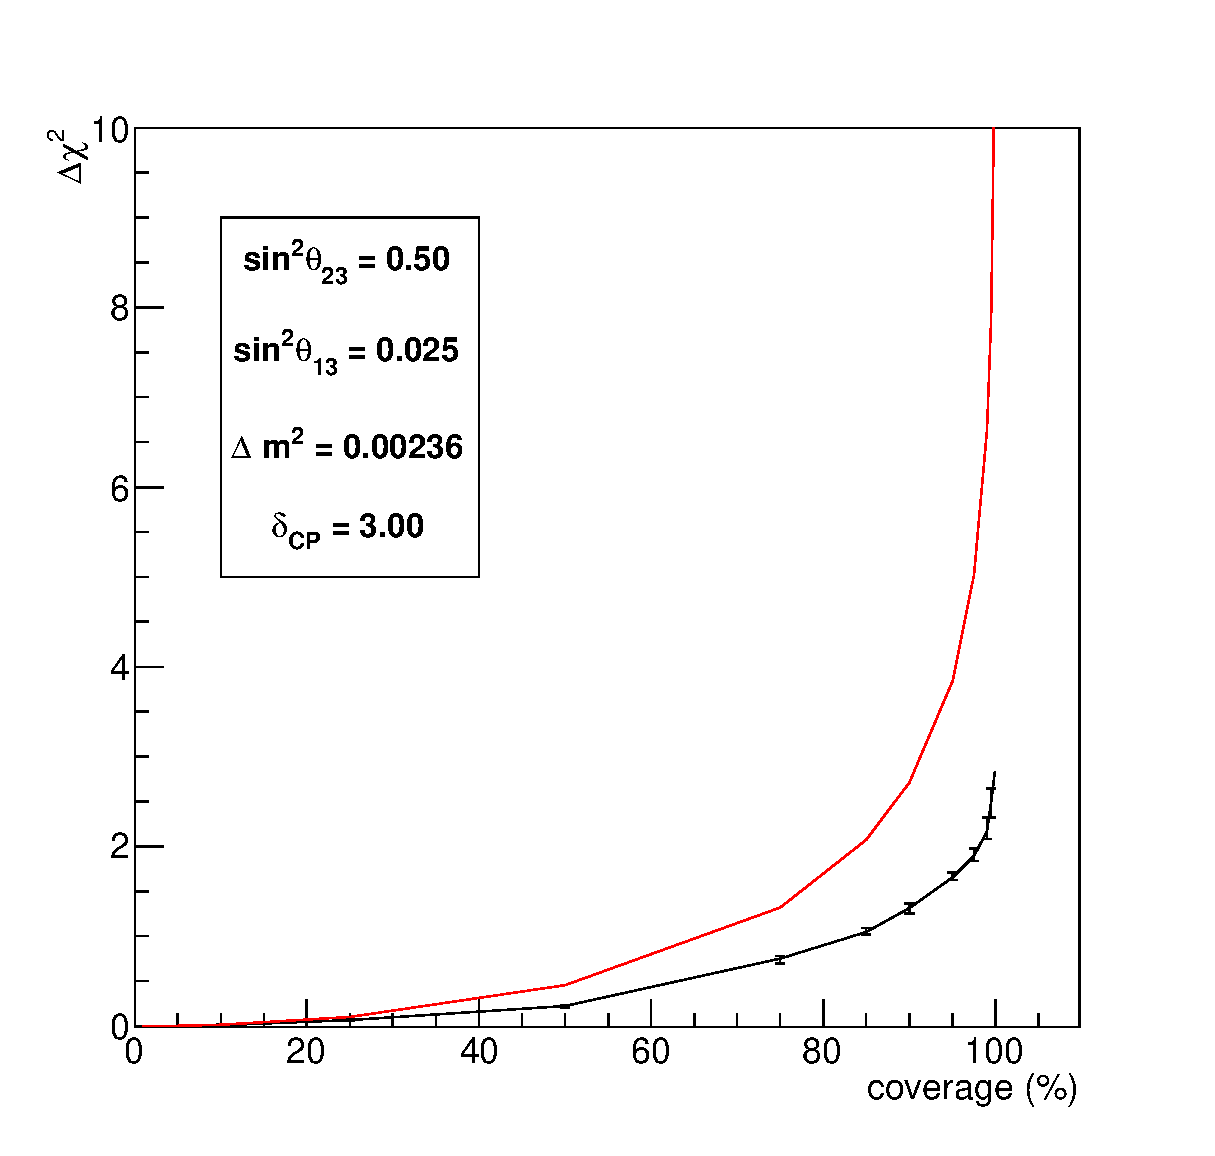
\includegraphics[width=14pc]{./images/appendix/coverage/coverage_study_1D_deltacp_3.eps}
\center
\caption {
  Distribution of $\Delta\chi^{2}$ vs coverage in the $\delta_{CP}$ parameter space
  from 1k toy MC experiments generated with the Run 1+2+3 POT
  with statistical fluctuations at the oscillation point indicated in the legend.
}
\label{fig:cov_1D_deltacp_3}
\end{minipage}
\hspace{0.03\linewidth}
\begin{minipage}[t]{0.46\linewidth}
\center
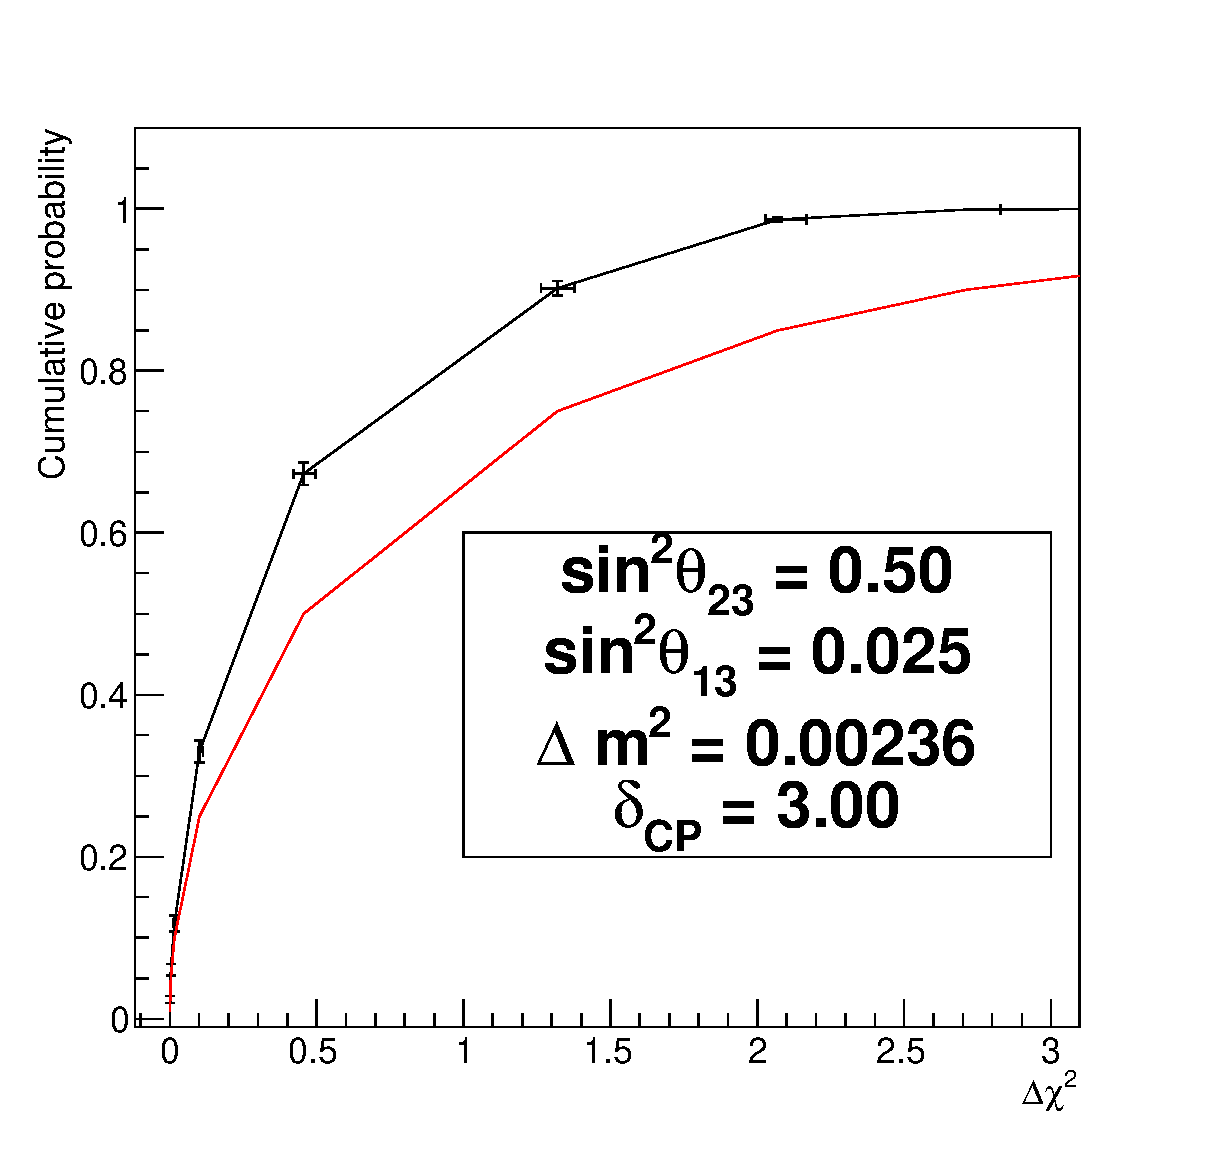
\includegraphics[width=14pc]{./images/appendix/coverage/coverage_study_1D_stats_deltacp_new_3.eps}
\center
\caption {
  Distribution of cumulative probability vs $\Delta\chi^{2}$ in the $\delta_{CP}$ parameter space
  from 1k toy MC experiments generated with the Run 1+2+3 POT
  with statistical fluctuations at the oscillation point indicated in the legend.
}
\label{fig:prob_1D_deltacp_3}
\end{minipage}
\vfill
\vspace*{0.7cm}
\begin{minipage}[t]{0.46\linewidth}
\center
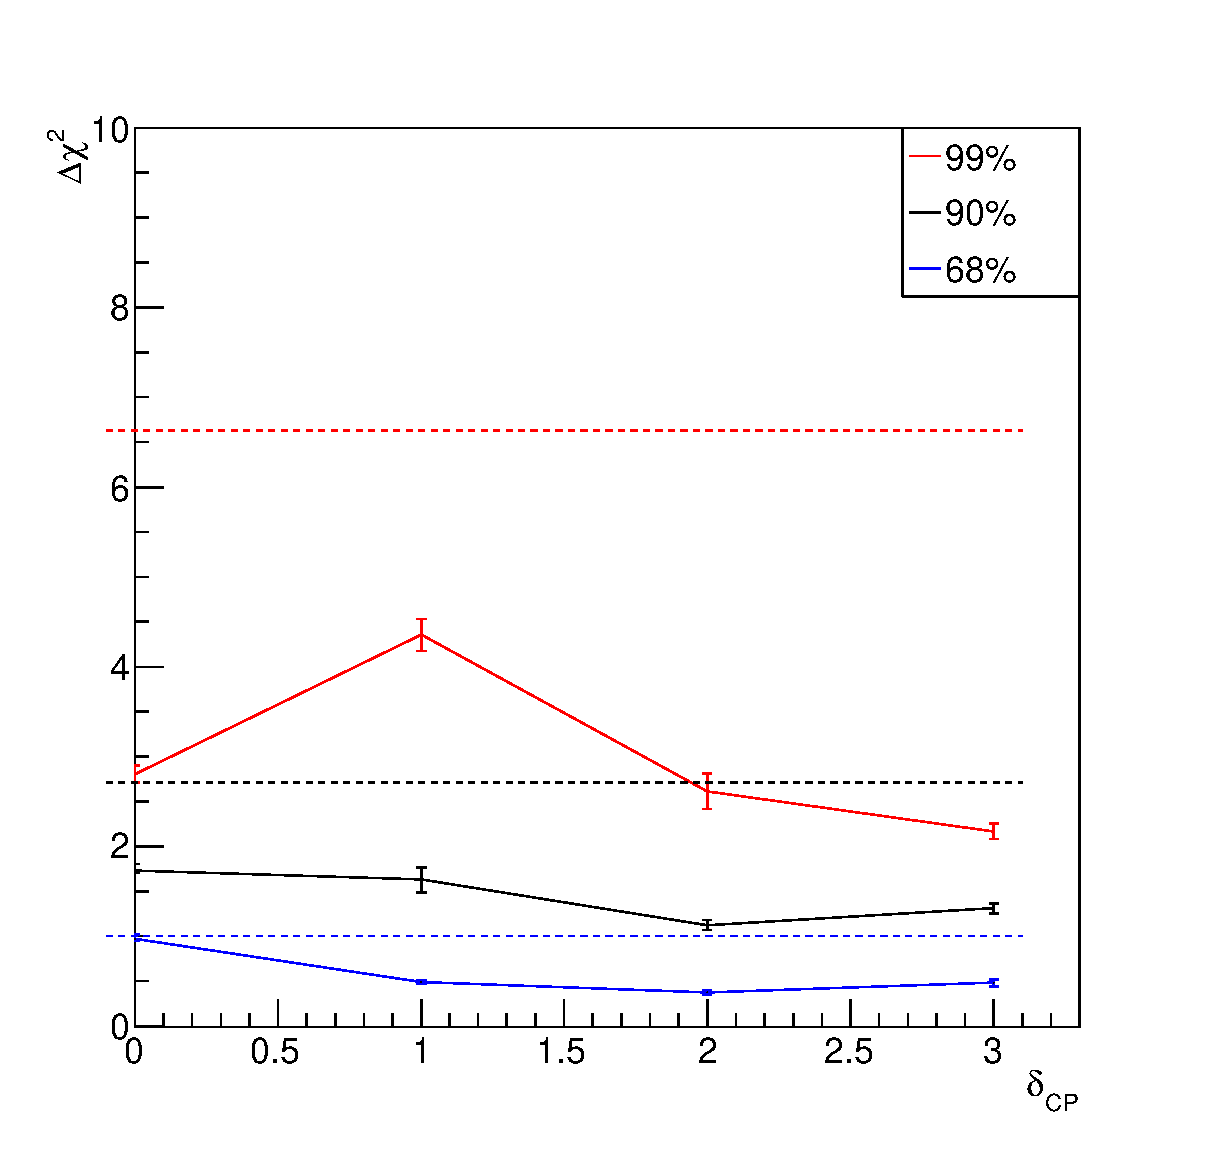
\includegraphics[width=14pc]{./images/appendix/coverage/coverage_study_1D_deltacp_all.eps}
\caption {
   Summary of figures \ref{fig:cov_1D_deltacp_0}-\ref{fig:cov_1D_deltacp_3}
showing the value of $\Delta\chi^{2}$ at 99\%, 90\% and 68\% confidence intervals vs the value of $\delta_{CP}$.
Horizontal dashed lines show the canonical $\Delta\chi^{2}$ value for 1 degree of freedom.
	}
\label{fig:cov_1D_deltacp_all}
\end{minipage}
\hspace{0.03\linewidth}
\begin{minipage}[t]{0.46\linewidth}
\center
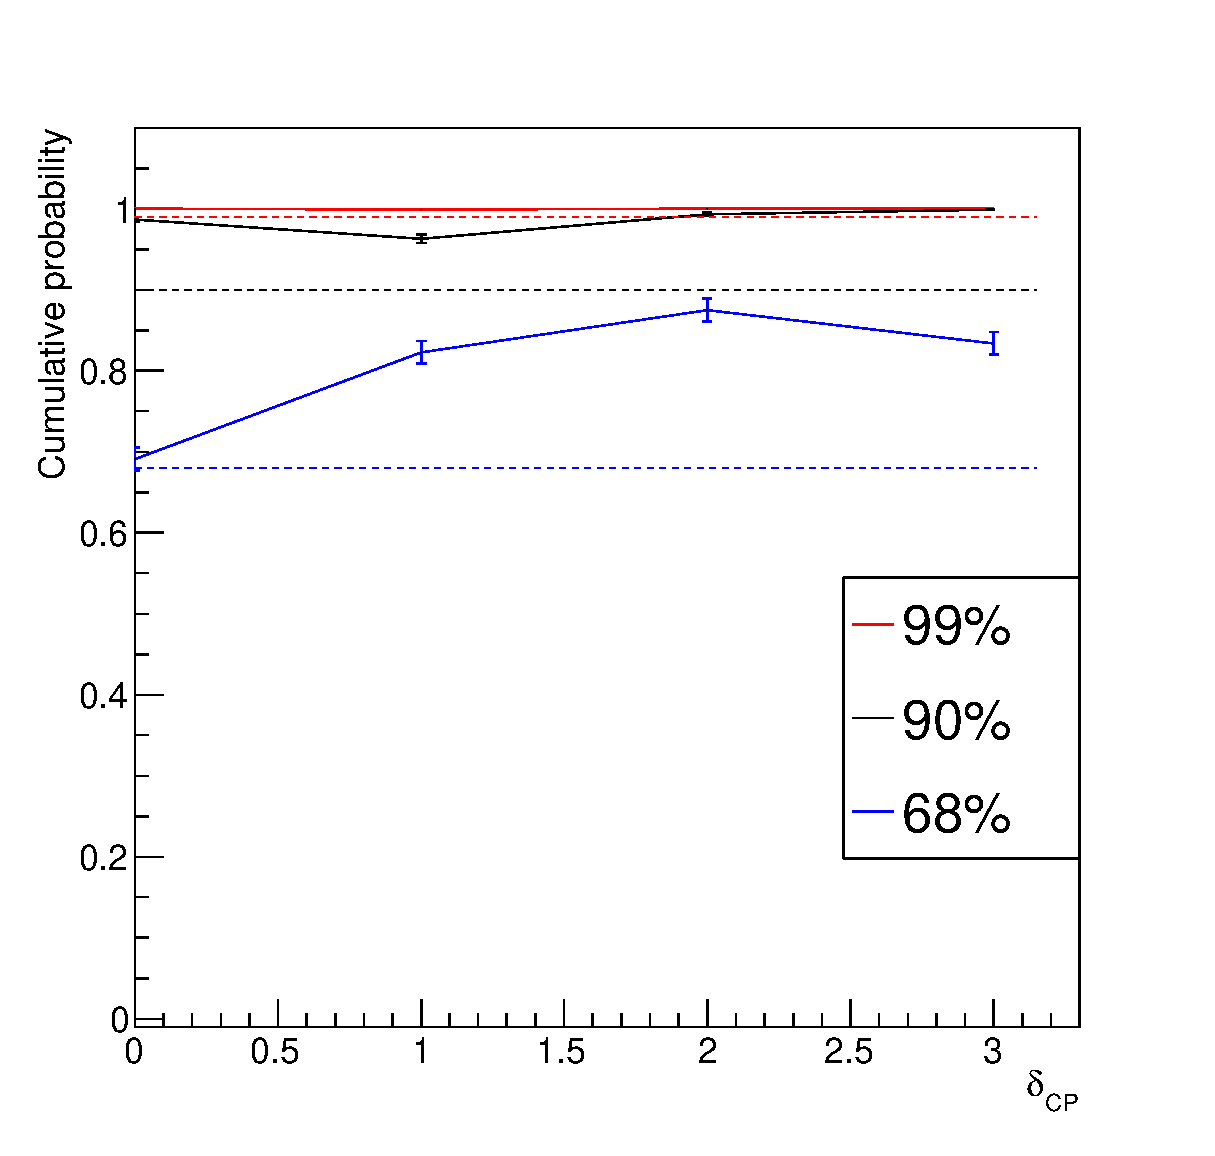
\includegraphics[width=14pc]{./images/appendix/coverage/coverage_study_1D_stats_deltacp_new_all.eps}
\caption {
Summary of figures \ref{fig:prob_1D_deltacp_0}-\ref{fig:prob_1D_deltacp_3}
showing the value of cumulative probability for $\Delta\chi^{2}=6.63$ (canonical value for 99\%), $\Delta\chi^{2}=2.71$ (canonical value for 90\%) and $\Delta\chi^{2}=1.0$ (canonical value for 68\%) vs the value of $\delta_{CP}$.
	}
\label{fig:prob_1D_deltacp_all}
\end{minipage}
\end{figure*}
\end{center}
\clearpage
\subsubsection{Coverage studies in 2D}
\label{app:cov:statonly:2d}
In this subsection the distribution of $\Delta\chi^{2}$ vs coverage is presented
for different oscillation points in the 2D parameter spaces where our results are presented,
overlaying the canonical $\Delta\chi^{2}$ pdf for 2 degrees of freedom (red lines). 
The procedure is the same described in previous subsection. 

Figures \ref{fig:cov_2D_theta23_dmsq_0}-\ref{fig:cov_2D_theta23_dmsq_3} show the distribution of $\Delta\chi^{2}$ vs coverage
in the 2D parameter space ($sin^{2}\theta_{23}$,$|\Delta m^{2}|$), calculated with 1k toy experiments with statistical fluctuations 
and fitting for $sin^{2}\theta_{23}$ and $|\Delta m^{2}|$, for different values of $sin^{2}\theta_{23}$ (to investigate the physical boundary concerning this parameter). 
In Fig. \ref{fig:cov_2D_theta23_dmsq_all} a summary of the previous plots is presented,
showing the value of $\Delta\chi^{2}$ at 99\%, 90\% and 68\% confidence intervals vs the value of $sin^{2}\theta_{23}$.

Figures \ref{fig:prob_2D_theta23_dmsq_0}-\ref{fig:prob_2D_theta23_dmsq_3} show the distribution of cumulative probability vs $\Delta\chi^{2}$
in the 2D parameter space ($sin^{2}\theta_{23}$,$|\Delta m^{2}|$), calculated with the same 1k toy experiments with statistical fluctuations 
and fitting for $sin^{2}\theta_{23}$ and $|\Delta m^{2}|$, for different values of $sin^{2}\theta_{23}$.
In Fig. \ref{fig:prob_2D_theta23_dmsq_all} a summary of the previous plots is presented,
showing the value of $\Delta\chi^{2}$ at 99\%, 90\% and 68\% confidence intervals vs the value of $sin^{2}\theta_{23}$.

Similarly for the 2D parameter space ($sin^{2}\theta_{13}$,$|\Delta m^{2}|$) in Figs. \ref{fig:cov_2D_theta13_dm23sq_0}-\ref{fig:cov_2D_theta13_dm23sq_all}.

The distributions for the parameter space ($sin^{2}\theta_{13}$,$\delta_{CP}$) are plotted differently,
including in Figs. \ref{fig:cov_2D_theta13_deltacp_0}-\ref{fig:cov_2D_theta13_deltacp_3} the canonical
$\Delta\chi^{2}$ pdf both for 2 degrees of freedom (red solid lines) and 1 degree of freedom (red dashed lines). 
In Fig. \ref{fig:cov_2D_theta13_deltacp_all} the lines with the canonical values of $\Delta\chi^{2}$ are also 
shown with different colors for 2 and 1 degrees of freedom (see legend). 
It is clear than in this special parameter space the distributions are closer to the ones corresponding to 1 degree
of freedom than the ones for the 2 degrees of freedom, indicating again than the behaviour of $\delta_{CP}$ is not like a real degree of freedom.

Finally in the distributions for the parameter space ($sin^{2}\theta_{13}$,$sin^{2}\theta_{23}$),
physical boundaries are present in both oscillation parameters so more grid points are to be studied 
with the combination of the selected values in the other 2D parameter spaces. 
Those distributions are presented in Figs. \ref{fig:cov_2D_theta13_theta23_0}-\ref{fig:cov_2D_theta13_theta23_19}
and a summary vs $sin^{2}\theta_{23}$ in Fig. \ref{fig:cov_2D_theta13_theta23_all_1} and vs  $sin^{2}\theta_{13}$ in Fig. \ref{fig:cov_2D_theta13_theta23_all_2}. Then a summary is presented with the value of $\Delta\chi^{2}$ in Z axis (color) vs $sin^{2}\theta_{23}$ in X axis and $sin^{2}\theta_{13}$ in Y axis at 68\% confidence interval in Fig.\ref{fig:cov_2D_theta13_theta23_68}, at 90\% confidence interval in Fig. \ref{fig:cov_2D_theta13_theta23_90} and at 99\%  confidence interval in Fig. \ref{fig:cov_2D_theta13_theta23_99}.

\begin{center}
\begin{figure*}[htb]
\begin{minipage}[t]{0.46\linewidth}
\center
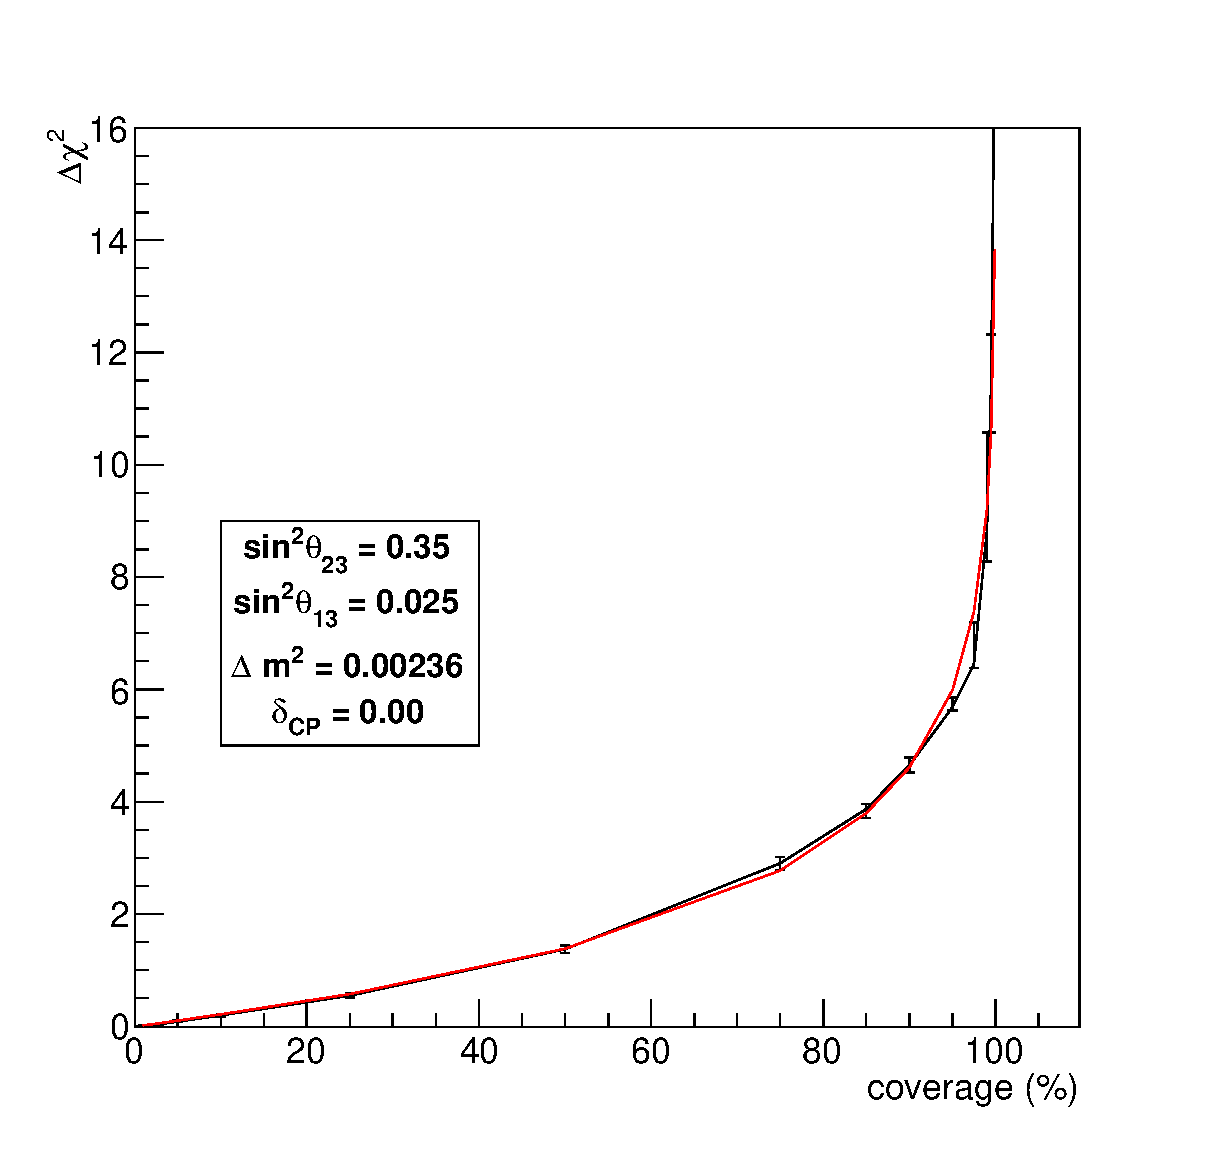
\includegraphics[width=14pc]{./images/appendix/coverage/coverage_study_2D_theta23_dm23sq_0.eps}
\center
\caption {
  Distribution of $\Delta\chi^{2}$ vs coverage in the ($sin^{2}\theta_{23}$,$|\Delta m^{2}|$) parameter space
  from 1k toy MC experiments generated with the Run 1+2+3 POT
  with statistical fluctuations at the oscillation point indicated in the legend.
}
\label{fig:cov_2D_theta23_dmsq_0}
\end{minipage}
\hspace{0.03\linewidth}
\begin{minipage}[t]{0.46\linewidth}
\center
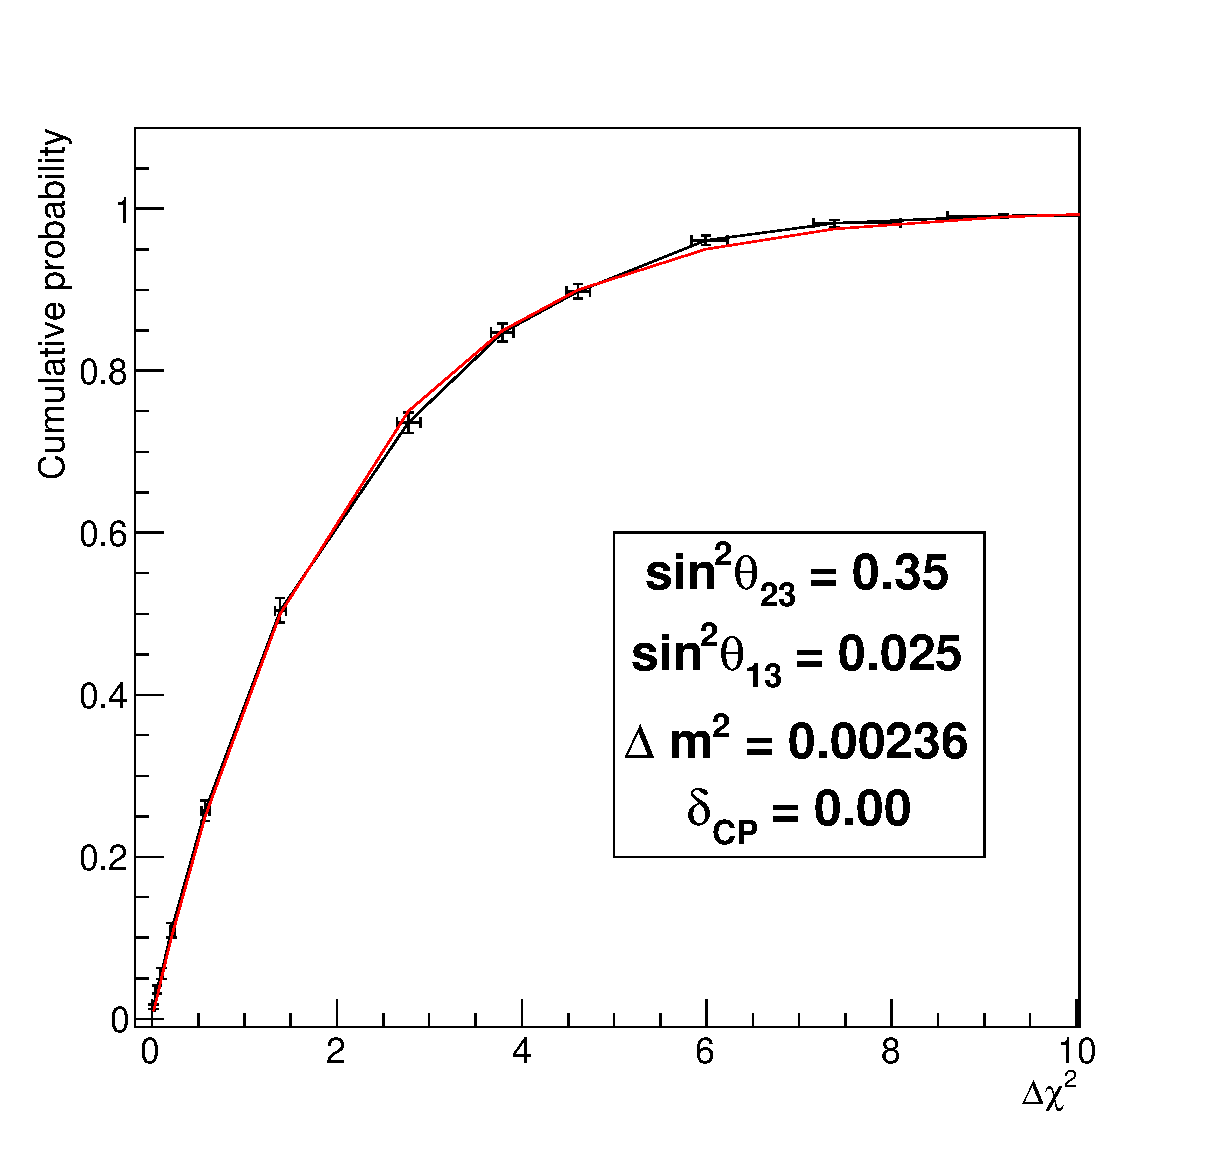
\includegraphics[width=14pc]{./images/appendix/coverage/coverage_study_2D_stats_theta23_dmsq_new_0.eps}
\center
\caption {
  Distribution of cumulative probability vs $\Delta\chi^{2}$ in the ($sin^{2}\theta_{23}$,$|\Delta m^{2}|$) parameter space
  from 1k toy MC experiments generated with the Run 1+2+3 POT
  with statistical fluctuations at the oscillation point indicated in the legend.
}
\label{fig:prob_2D_theta23_dmsq_0}
\end{minipage}
\vfill
\vspace*{0.7cm}
\begin{minipage}[t]{0.46\linewidth}
\center
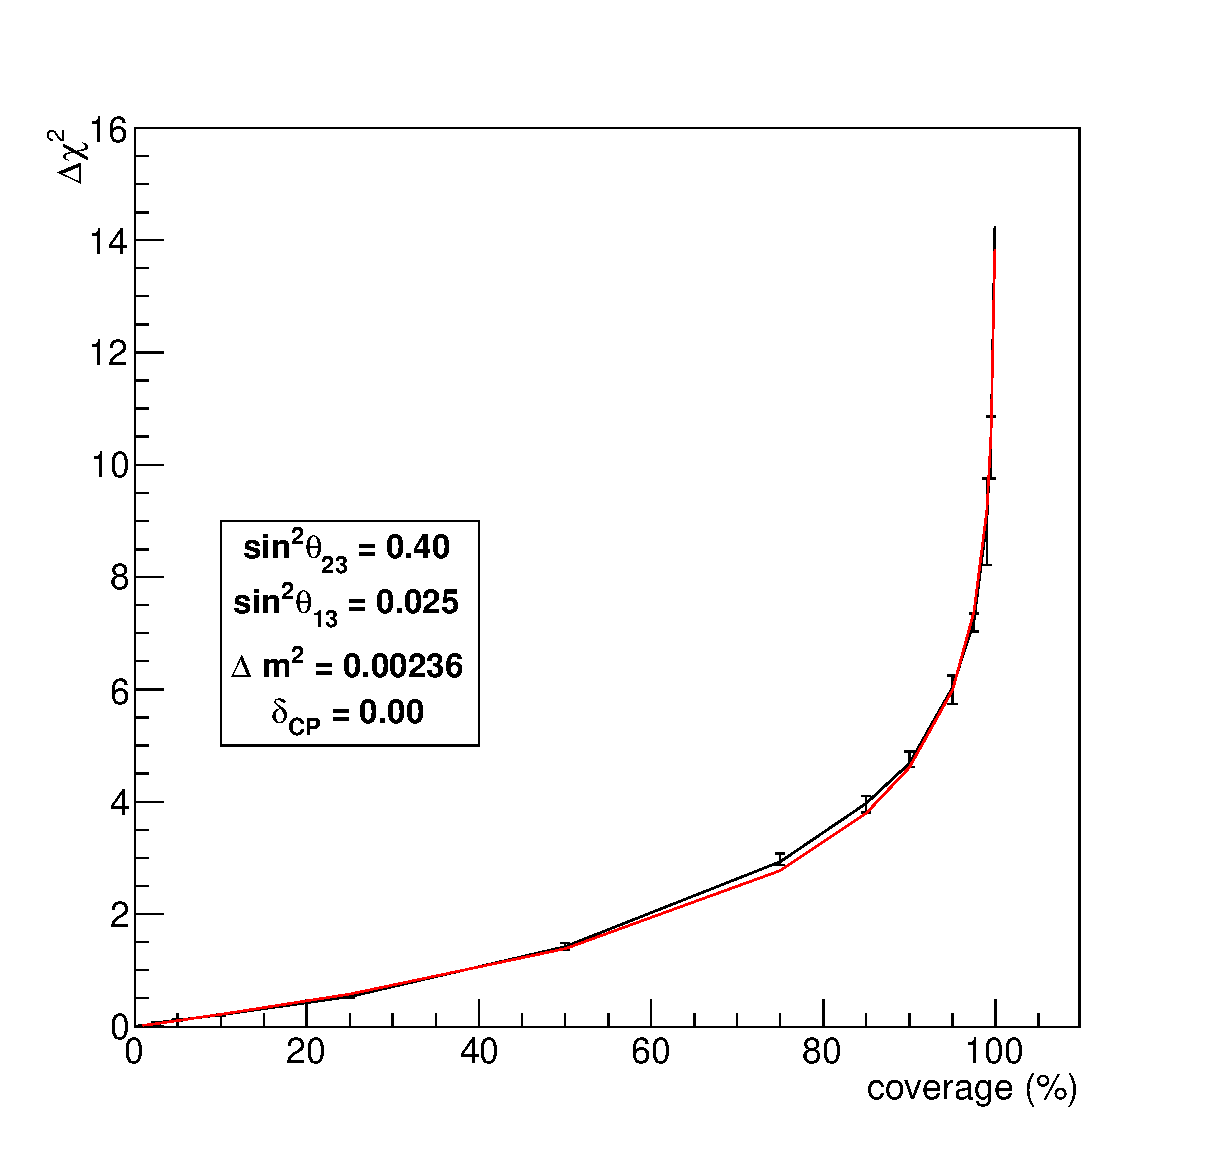
\includegraphics[width=14pc]{./images/appendix/coverage/coverage_study_2D_theta23_dm23sq_1.eps}
\center
\caption {
  Distribution of $\Delta\chi^{2}$ vs coverage in the ($sin^{2}\theta_{23}$,$|\Delta m^{2}|$) parameter space
  from 1k toy MC experiments generated with the Run 1+2+3 POT
  with statistical fluctuations at the oscillation point indicated in the legend.
}
\label{fig:cov_2D_theta23_dmsq_1}
\end{minipage}
\hspace{0.03\linewidth}
\begin{minipage}[t]{0.46\linewidth}
\center
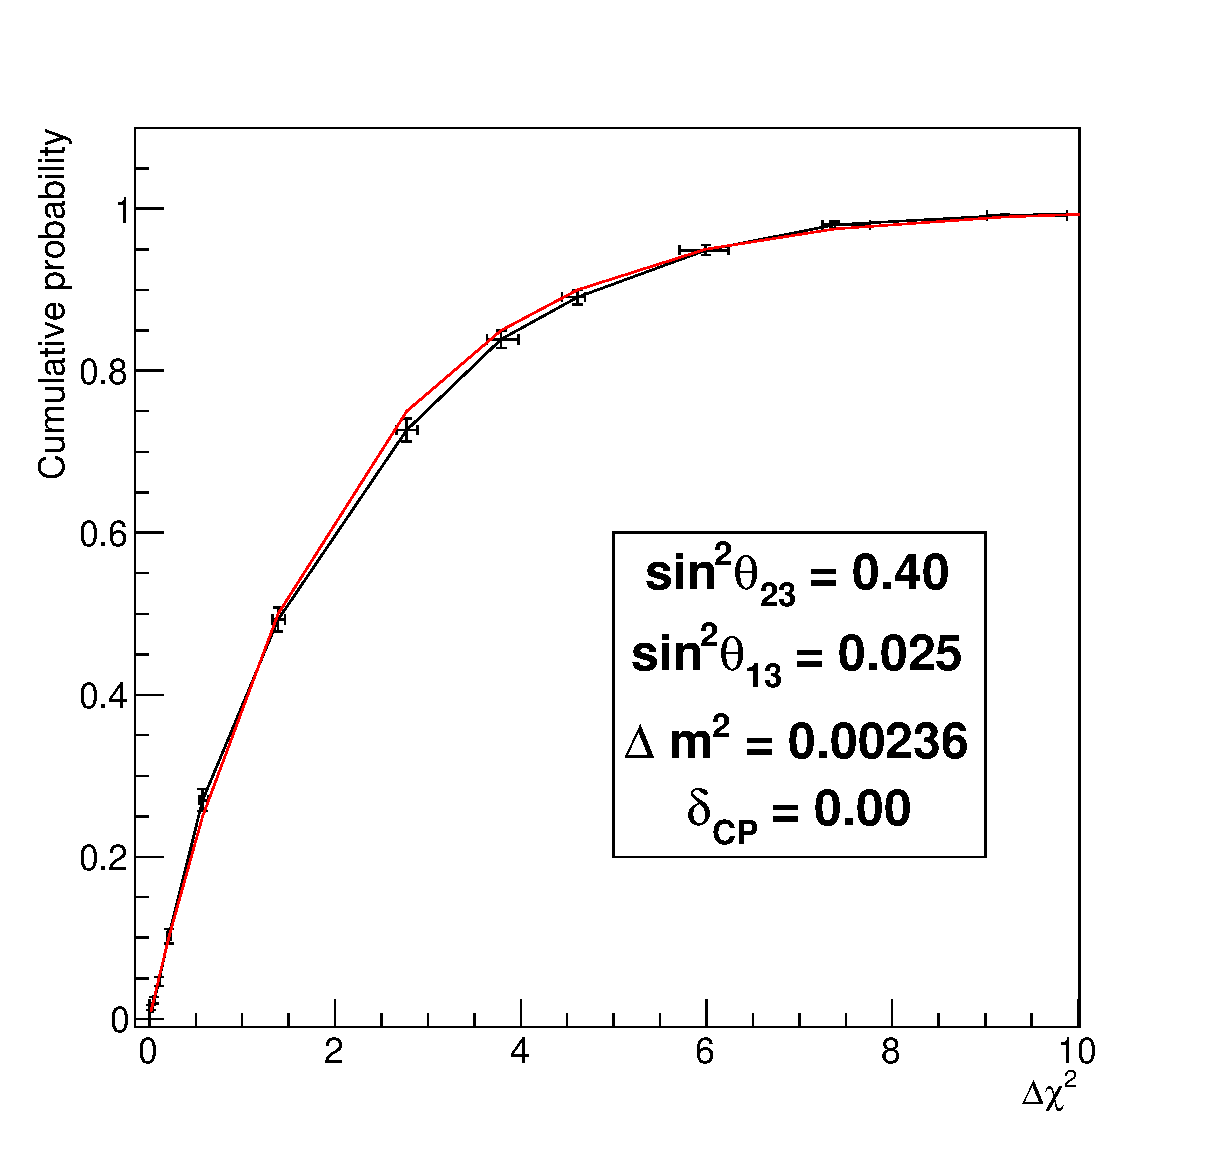
\includegraphics[width=14pc]{./images/appendix/coverage/coverage_study_2D_stats_theta23_dmsq_new_1.eps}
\center
\caption {
  Distribution of cumulative probability vs $\Delta\chi^{2}$ in the ($sin^{2}\theta_{23}$,$|\Delta m^{2}|$) parameter space
  from 1k toy MC experiments generated with the Run 1+2+3 POT
  with statistical fluctuations at the oscillation point indicated in the legend.
}
\label{fig:prob_2D_theta23_dmsq_1}
\end{minipage}
\vfill
\vspace*{0.7cm}
\begin{minipage}[t]{0.46\linewidth}
\center
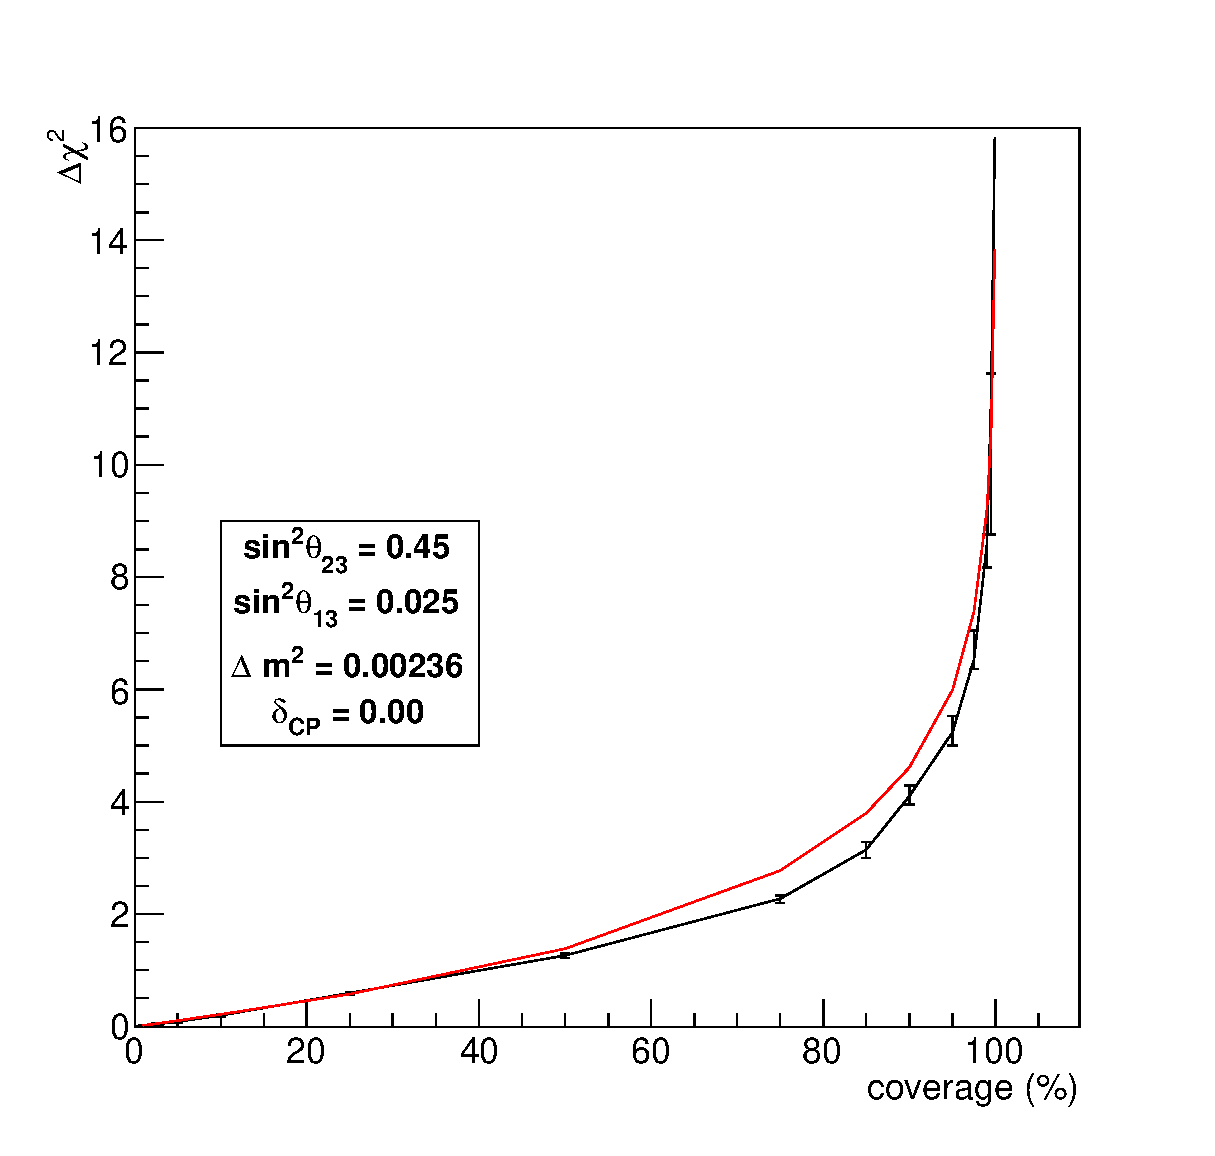
\includegraphics[width=14pc]{./images/appendix/coverage/coverage_study_2D_theta23_dm23sq_2.eps}
\center
\caption {
  Distribution of $\Delta\chi^{2}$ vs coverage in the ($sin^{2}\theta_{23}$,$|\Delta m^{2}|$) parameter space
  from 1k toy MC experiments generated with the Run 1+2+3 POT
  with statistical fluctuations at the oscillation point indicated in the legend.
}
\label{fig:cov_2D_theta23_dmsq_2}
\end{minipage}
\hspace{0.03\linewidth}
\begin{minipage}[t]{0.46\linewidth}
\center
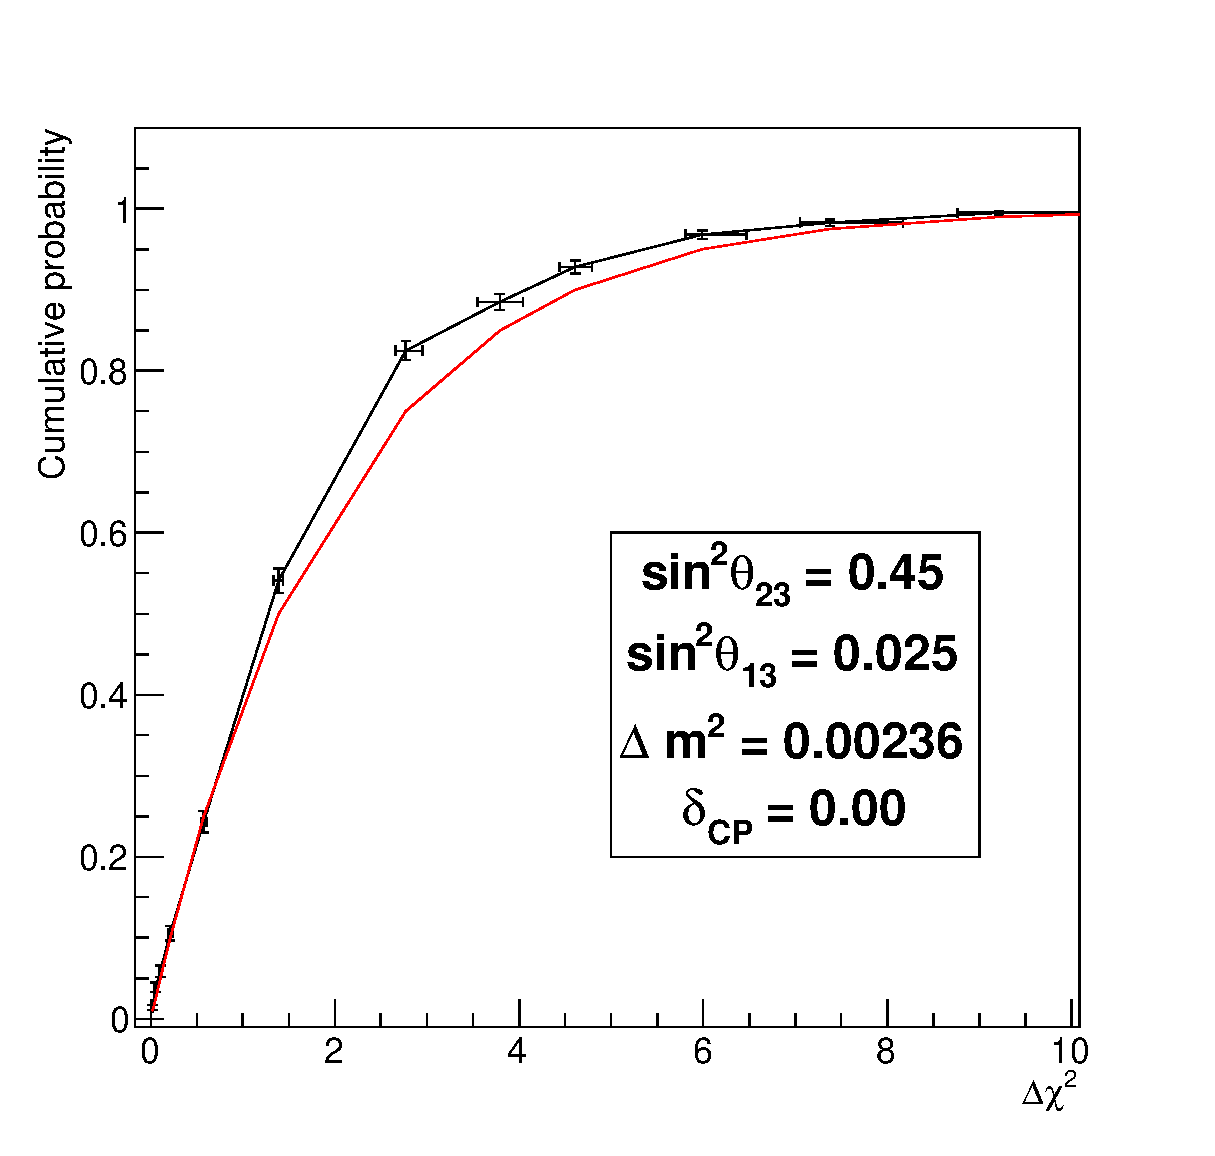
\includegraphics[width=14pc]{./images/appendix/coverage/coverage_study_2D_stats_theta23_dmsq_new_2.eps}
\center
\caption {
  Distribution of cumulative probability vs $\Delta\chi^{2}$ in the ($sin^{2}\theta_{23}$,$|\Delta m^{2}|$) parameter space
  from 1k toy MC experiments generated with the Run 1+2+3 POT
  with statistical fluctuations at the oscillation point indicated in the legend.
}
\label{fig:prob_2D_theta23_dmsq_2}
\end{minipage}
\end{figure*}
\end{center}

\begin{center}
\begin{figure*}[htb]
\begin{minipage}[t]{0.46\linewidth}
\center
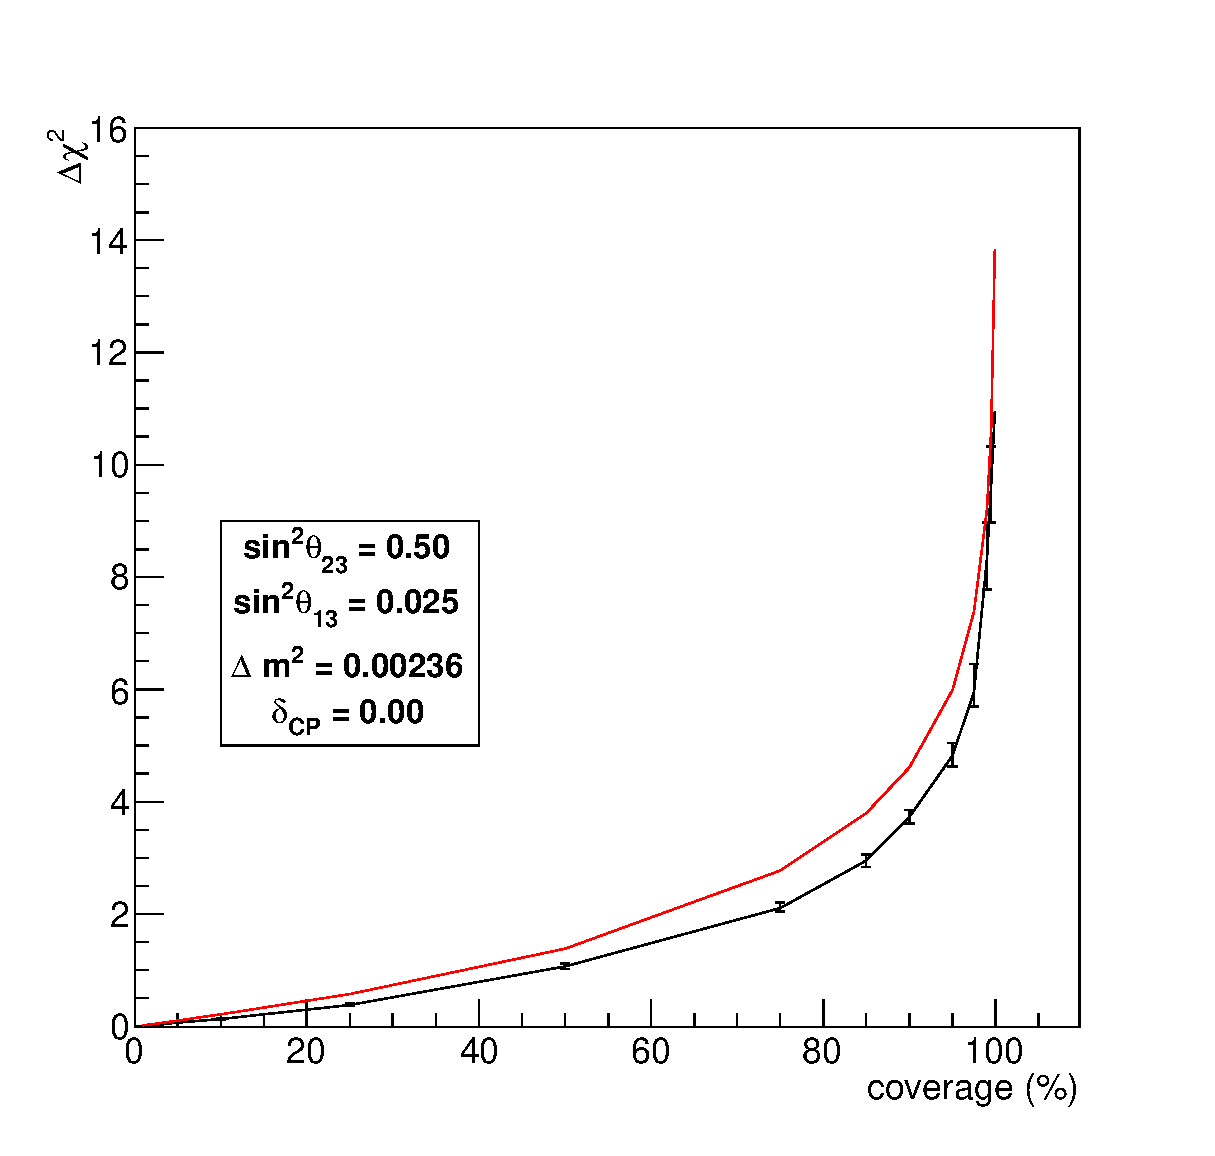
\includegraphics[width=14pc]{./images/appendix/coverage/coverage_study_2D_theta23_dm23sq_3.eps}
\center
\caption {
  Distribution of $\Delta\chi^{2}$ vs coverage in the ($sin^{2}\theta_{23}$,$|\Delta m^{2}|$) parameter space
  from 1k toy MC experiments generated with the Run 1+2+3 POT
  with statistical fluctuations at the oscillation point indicated in the legend.
}
\label{fig:cov_2D_theta23_dmsq_3}
\end{minipage}
\hspace{0.03\linewidth}
\begin{minipage}[t]{0.46\linewidth}
\center
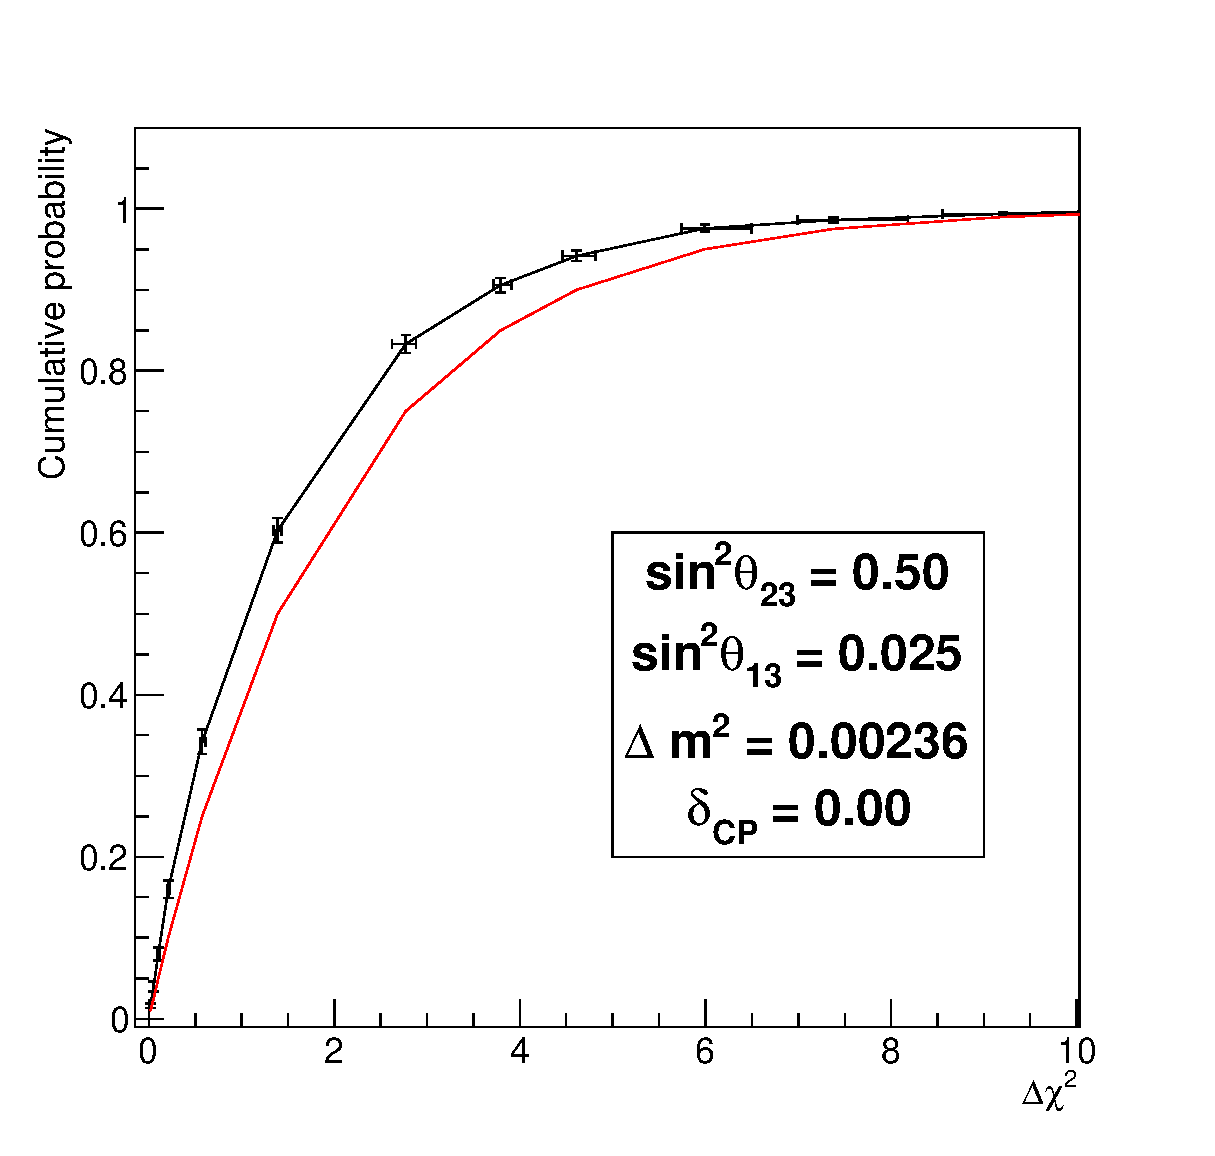
\includegraphics[width=14pc]{./images/appendix/coverage/coverage_study_2D_stats_theta23_dmsq_new_3.eps}
\center
\caption {
  Distribution of cumulative probability vs $\Delta\chi^{2}$ in the ($sin^{2}\theta_{23}$,$|\Delta m^{2}|$) parameter space
  from 1k toy MC experiments generated with the Run 1+2+3 POT
  with statistical fluctuations at the oscillation point indicated in the legend.
}
\label{fig:prob_2D_theta23_dmsq_3}
\end{minipage}
\vfill
\vspace*{0.7cm}
\begin{minipage}[t]{0.46\linewidth}
\center
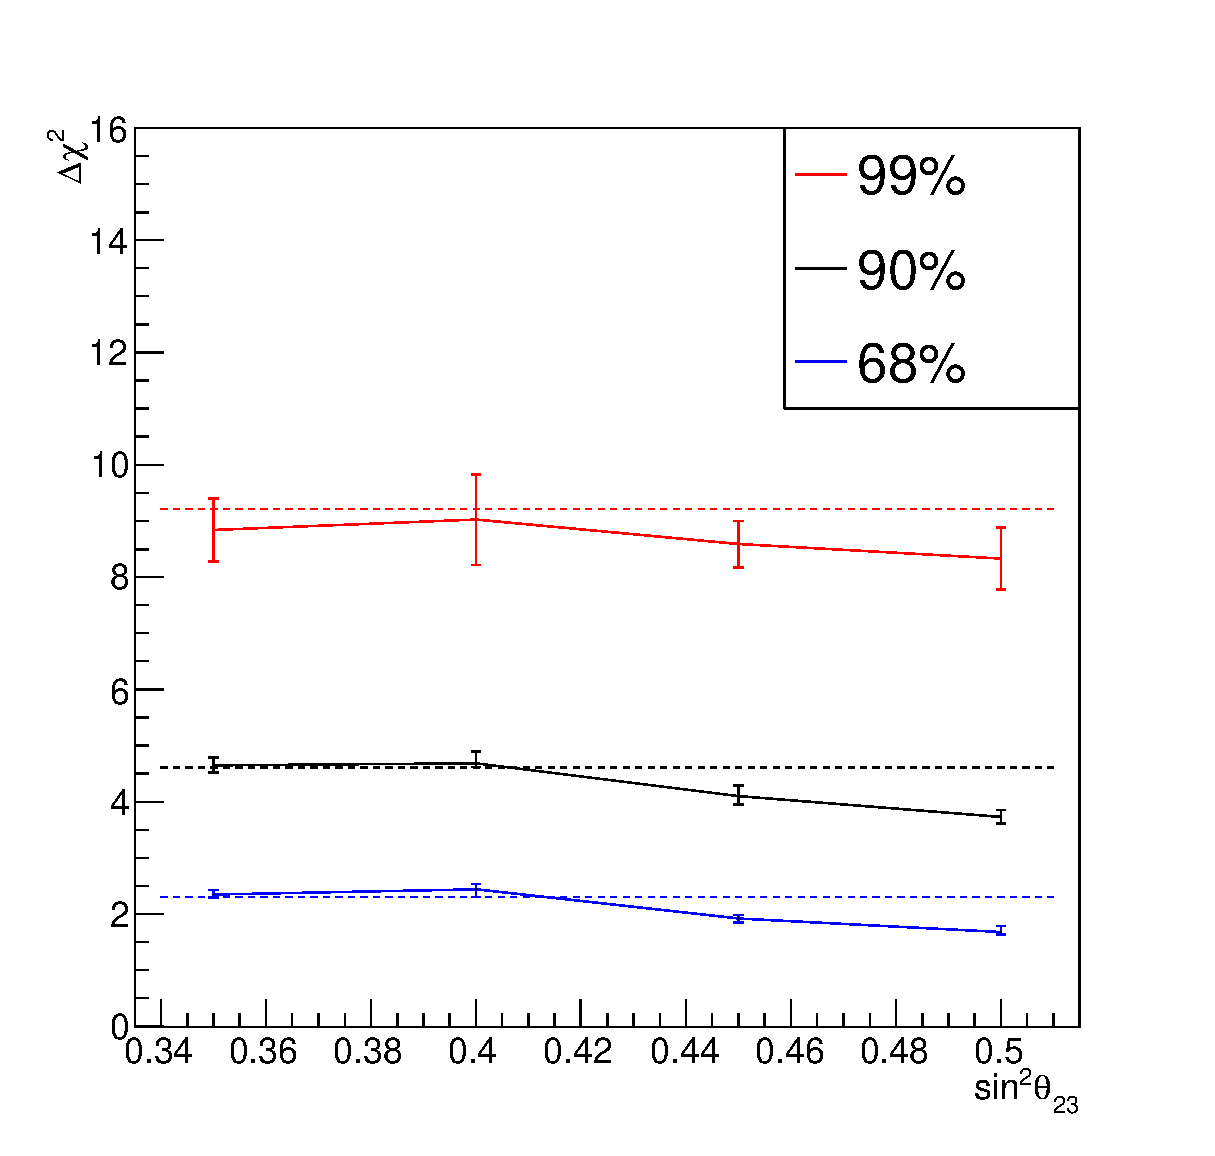
\includegraphics[width=14pc]{./images/appendix/coverage/coverage_study_2D_theta23_dm23sq_all.eps}
\caption {
   Summary of figures \ref{fig:cov_2D_theta23_dmsq_0}-\ref{fig:cov_2D_theta23_dmsq_3}
showing the value of $\Delta\chi^{2}$ at 99\%, 90\% and 68\% confidence intervals vs the value of $sin^{2}\theta_{23}$.
Horizontal dashed lines show the canonical $\Delta\chi^{2}$ value for 2 degrees of freedom.
	}
\label{fig:cov_2D_theta23_dmsq_all}
\end{minipage}
\hspace{0.03\linewidth}
\begin{minipage}[t]{0.46\linewidth}
\center
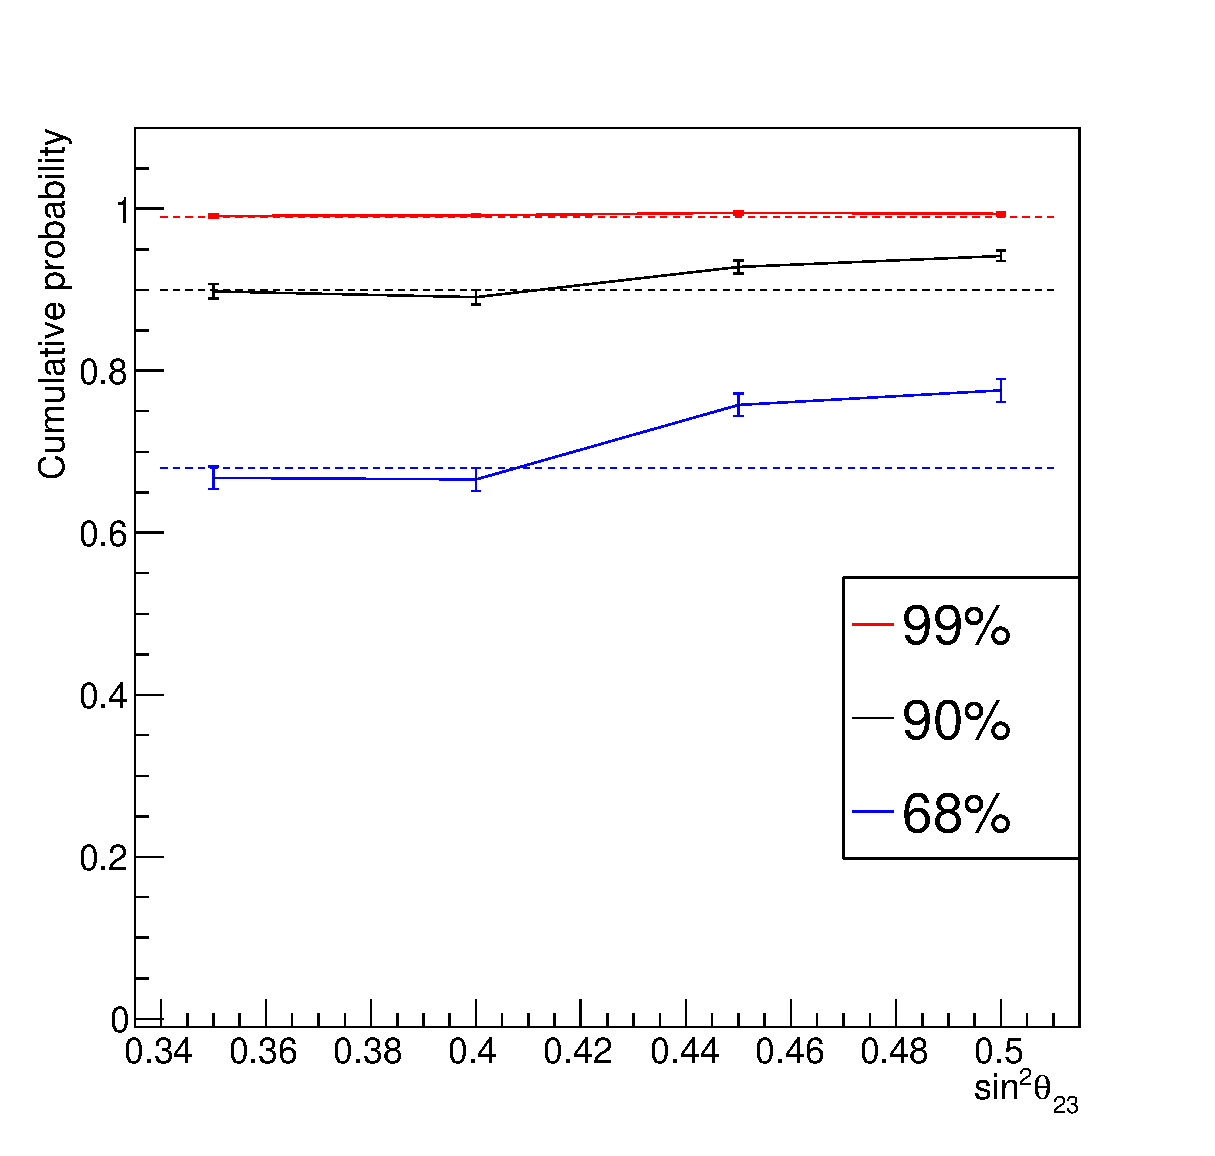
\includegraphics[width=14pc]{./images/appendix/coverage/coverage_study_2D_stats_theta23_dmsq_new_all.eps}
\caption {
	Summary of figures \ref{fig:prob_2D_theta23_dmsq_0}-\ref{fig:prob_2D_theta23_dmsq_3}
showing the value of cumulative probability for $\Delta\chi^{2}=9.21$ (canonical value for 99\%), $\Delta\chi^{2}=4.61$ (canonical value for 90\%) and $\Delta\chi^{2}=2.30$ (canonical value for 68\%) vs the value of $sin^{2}\theta_{23}$.
	}
\label{fig:prob_2D_theta23_dmsq_all}
\end{minipage}
\end{figure*}
\end{center}


%% FIGURES FOR 2D theta13-dmsq

\begin{center}
\begin{figure*}[htb]
\begin{minipage}[t]{0.46\linewidth}
\center
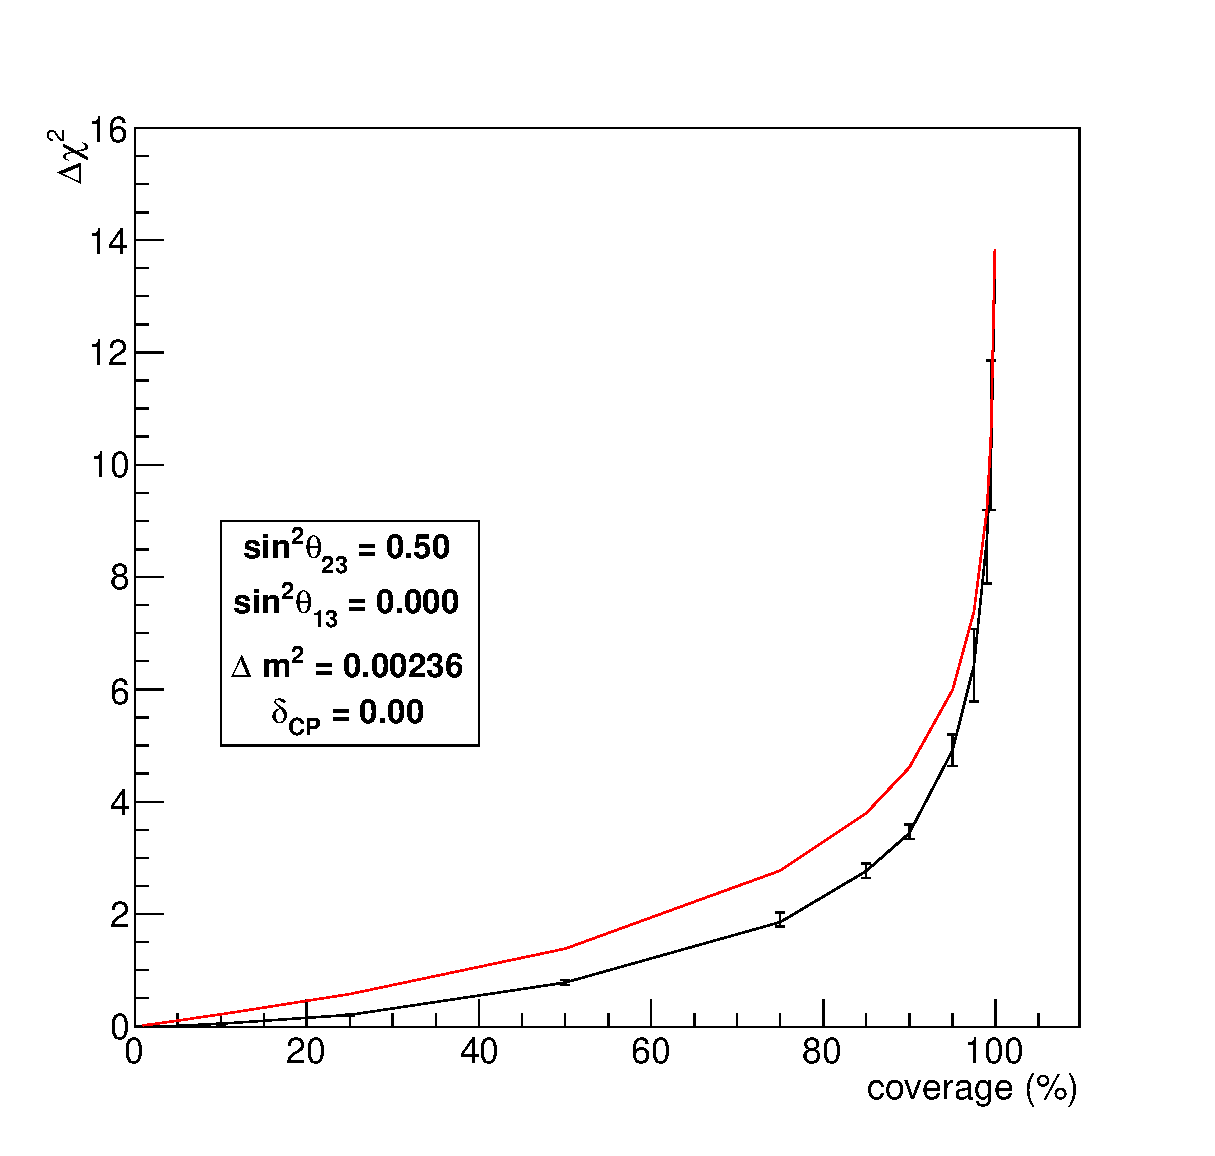
\includegraphics[width=14pc]{./images/appendix/coverage/coverage_study_2D_theta13_dm23sq_0.eps}
\center
\caption {
  Distribution of $\Delta\chi^{2}$ vs coverage in the ($sin^{2}\theta_{13}$,$|\Delta m^{2}|$) parameter space
  from 1k toy MC experiments generated with the Run 1+2+3 POT
  with statistical fluctuations at the oscillation point indicated in the legend.
}
\label{fig:cov_2D_theta13_dm23sq_0}
\end{minipage}
\hspace{0.03\linewidth}
\begin{minipage}[t]{0.46\linewidth}
\center
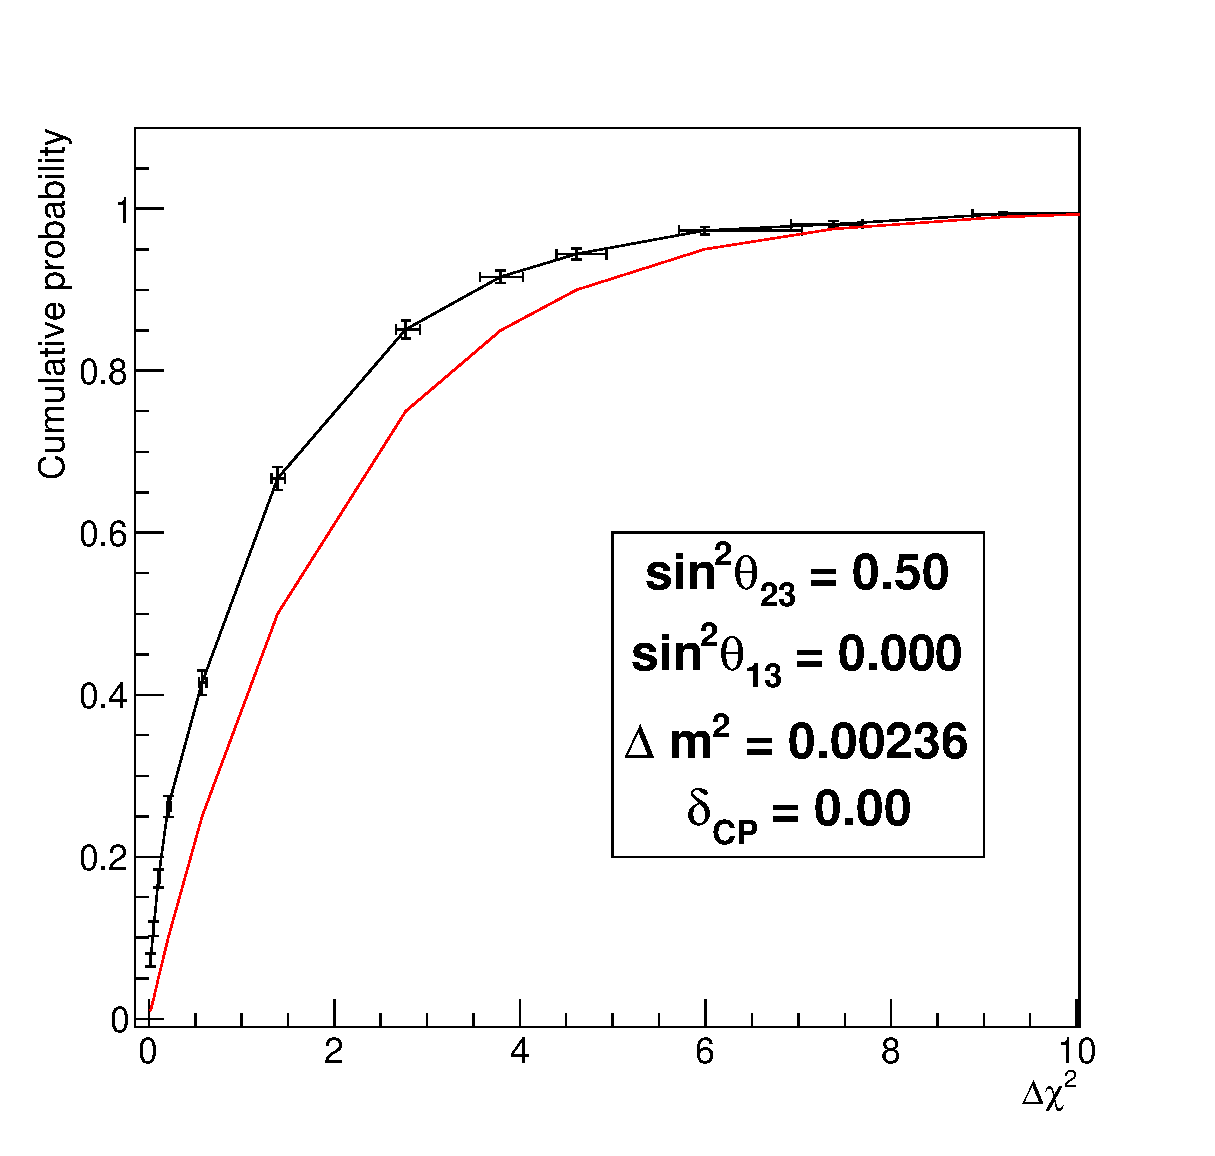
\includegraphics[width=14pc]{./images/appendix/coverage/coverage_study_2D_stats_theta13_dmsq_new_0.eps}
\center
\caption {
  Distribution of cumulative probability vs $\Delta\chi^{2}$ in the ($sin^{2}\theta_{13}$,$|\Delta m^{2}|$) parameter space
  from 1k toy MC experiments generated with the Run 1+2+3 POT
  with statistical fluctuations at the oscillation point indicated in the legend.
}
\label{fig:prob_2D_theta13_dm23sq_0}
\end{minipage}
\vfill
\vspace*{0.7cm}
\begin{minipage}[t]{0.46\linewidth}
\center
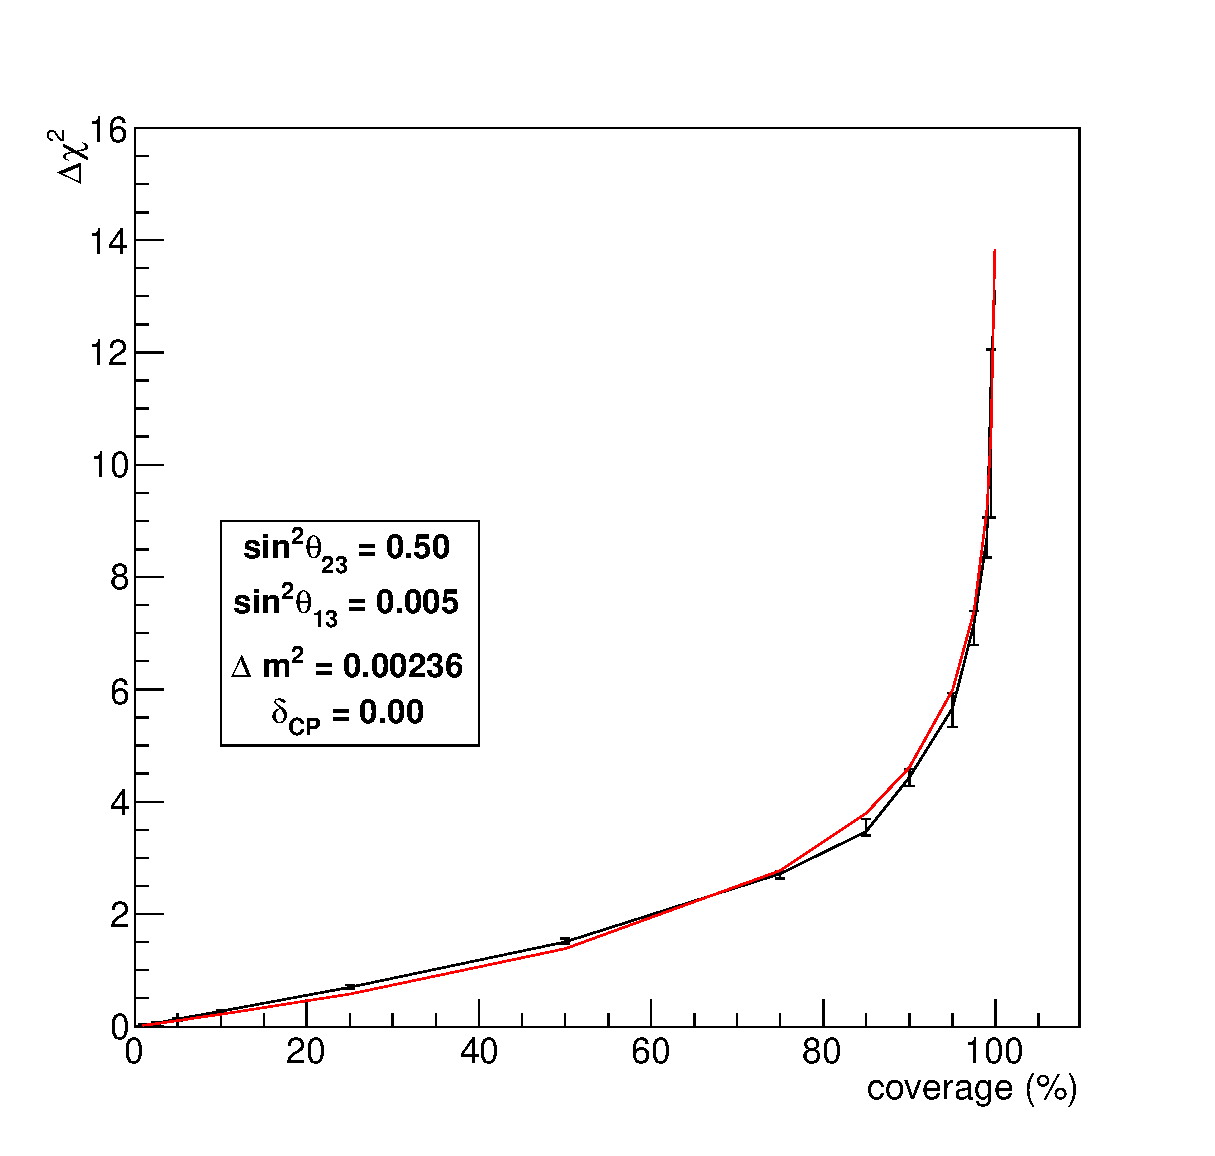
\includegraphics[width=14pc]{./images/appendix/coverage/coverage_study_2D_theta13_dm23sq_1.eps}
\center
\caption {
  Distribution of $\Delta\chi^{2}$ vs coverage in the ($sin^{2}\theta_{13}$,$|\Delta m^{2}|$) parameter space
  from 1k toy MC experiments generated with the Run 1+2+3 POT
  with statistical fluctuations at the oscillation point indicated in the legend.
}
\label{fig:cov_2D_theta13_dm23sq_1}
\end{minipage}
\hspace{0.03\linewidth}
\begin{minipage}[t]{0.46\linewidth}
\center
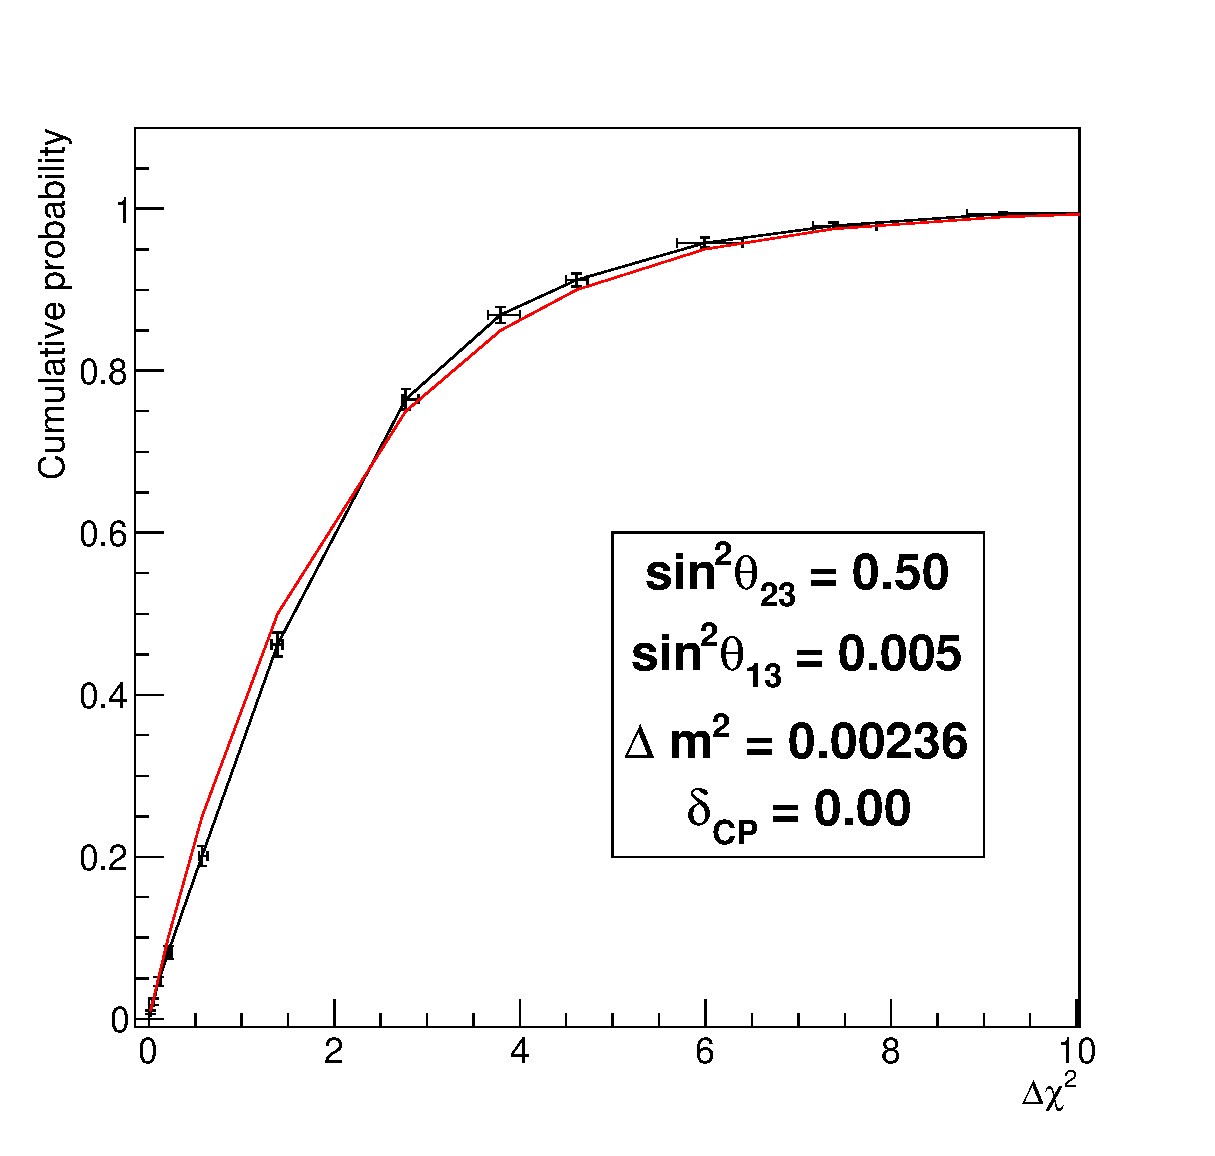
\includegraphics[width=14pc]{./images/appendix/coverage/coverage_study_2D_stats_theta13_dmsq_new_1.eps}
\center
\caption {
  Distribution of cumulative probability vs $\Delta\chi^{2}$ in the ($sin^{2}\theta_{13}$,$|\Delta m^{2}|$) parameter space
  from 1k toy MC experiments generated with the Run 1+2+3 POT
  with statistical fluctuations at the oscillation point indicated in the legend.
}
\label{fig:prob_2D_theta13_dm23sq_1}
\end{minipage}
\vfill
\vspace*{0.7cm}
\begin{minipage}[t]{0.46\linewidth}
\center
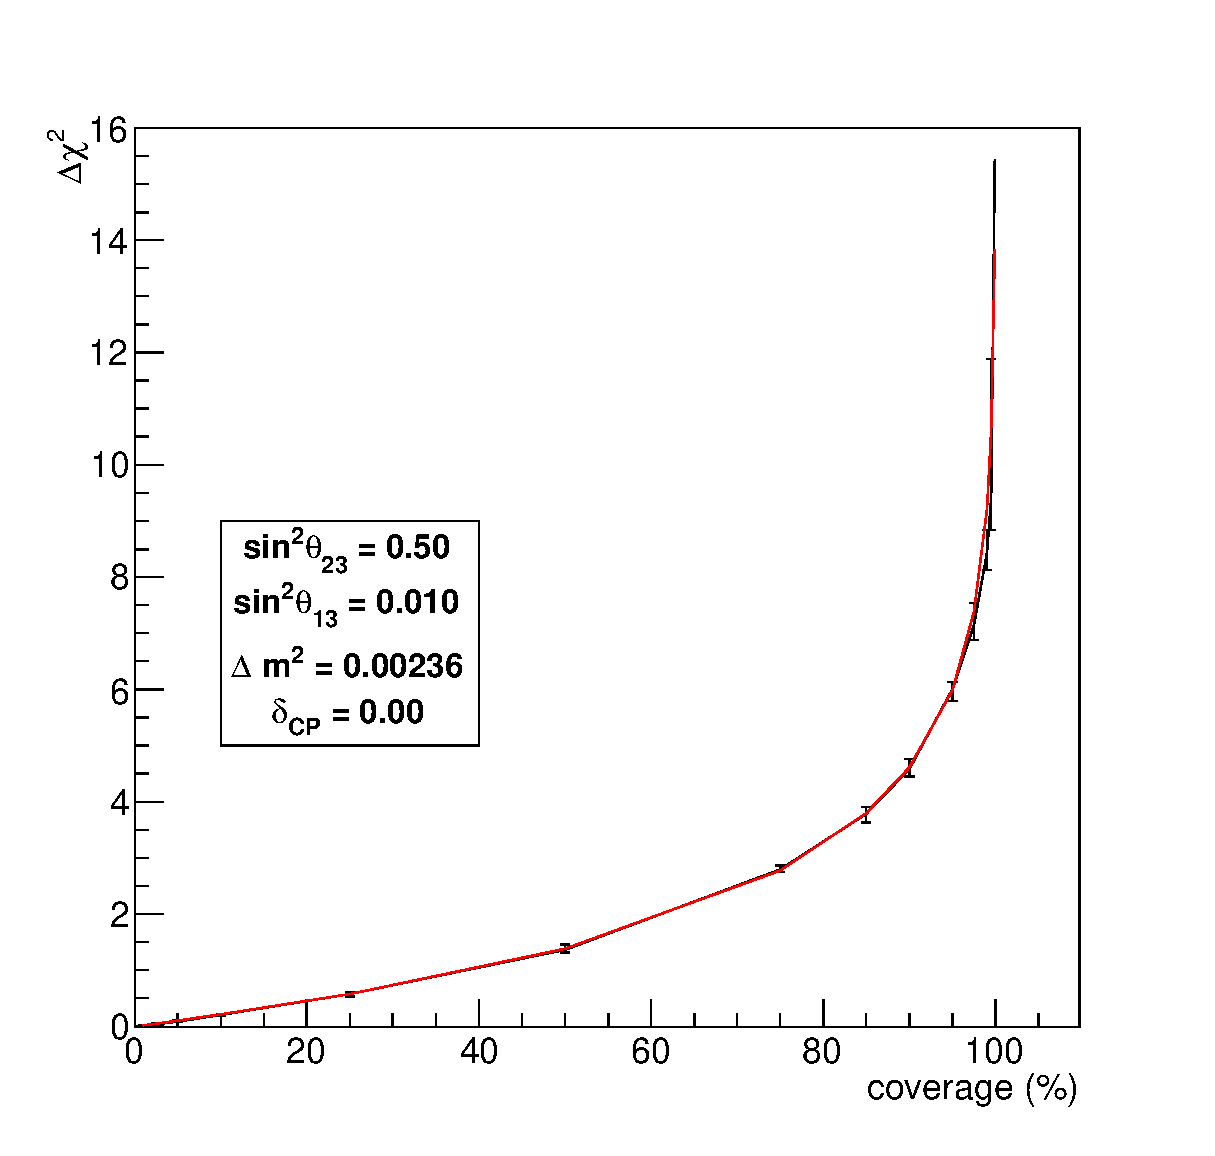
\includegraphics[width=14pc]{./images/appendix/coverage/coverage_study_2D_theta13_dm23sq_2.eps}
\center
\caption {
  Distribution of $\Delta\chi^{2}$ vs coverage in the ($sin^{2}\theta_{13}$,$|\Delta m^{2}|$) parameter space
  from 1k toy MC experiments generated with the Run 1+2+3 POT
  with statistical fluctuations at the oscillation point indicated in the legend.
}
\label{fig:cov_2D_theta13_dm23sq_2}
\end{minipage}
\hspace{0.03\linewidth}
\begin{minipage}[t]{0.46\linewidth}
\center
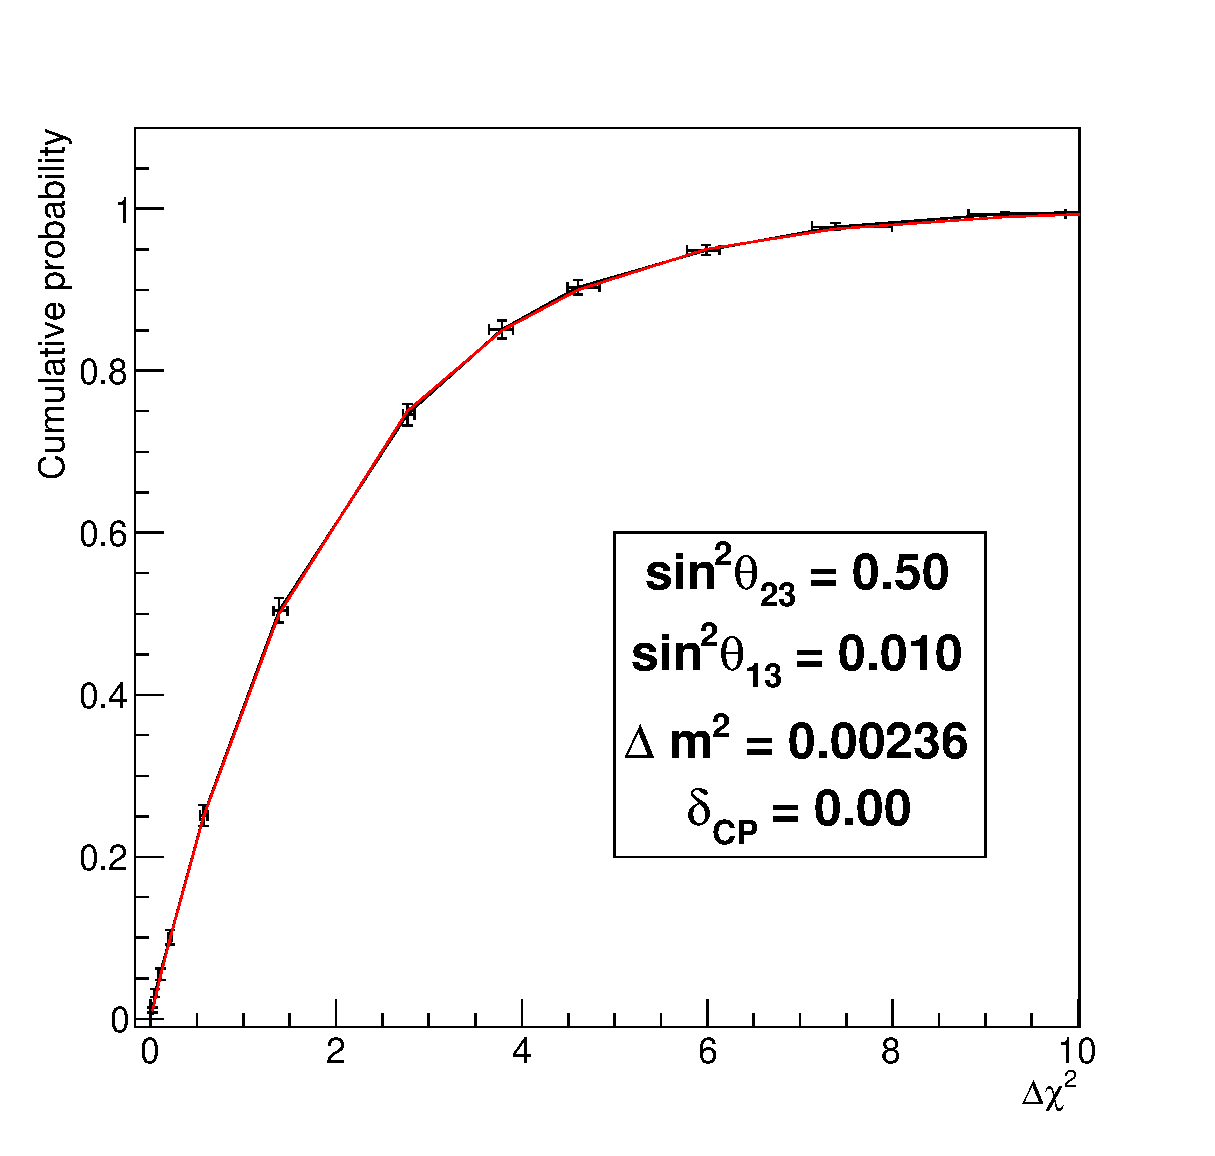
\includegraphics[width=14pc]{./images/appendix/coverage/coverage_study_2D_stats_theta13_dmsq_new_2.eps}
\center
\caption {
  Distribution of cumulative probability vs $\Delta\chi^{2}$ in the ($sin^{2}\theta_{13}$,$|\Delta m^{2}|$) parameter space
  from 1k toy MC experiments generated with the Run 1+2+3 POT
  with statistical fluctuations at the oscillation point indicated in the legend.
}
\label{fig:prob_2D_theta13_dm23sq_2}
\end{minipage}
\end{figure*}
\end{center}

\begin{center}
\begin{figure*}[htb]
\begin{minipage}[t]{0.46\linewidth}
\center
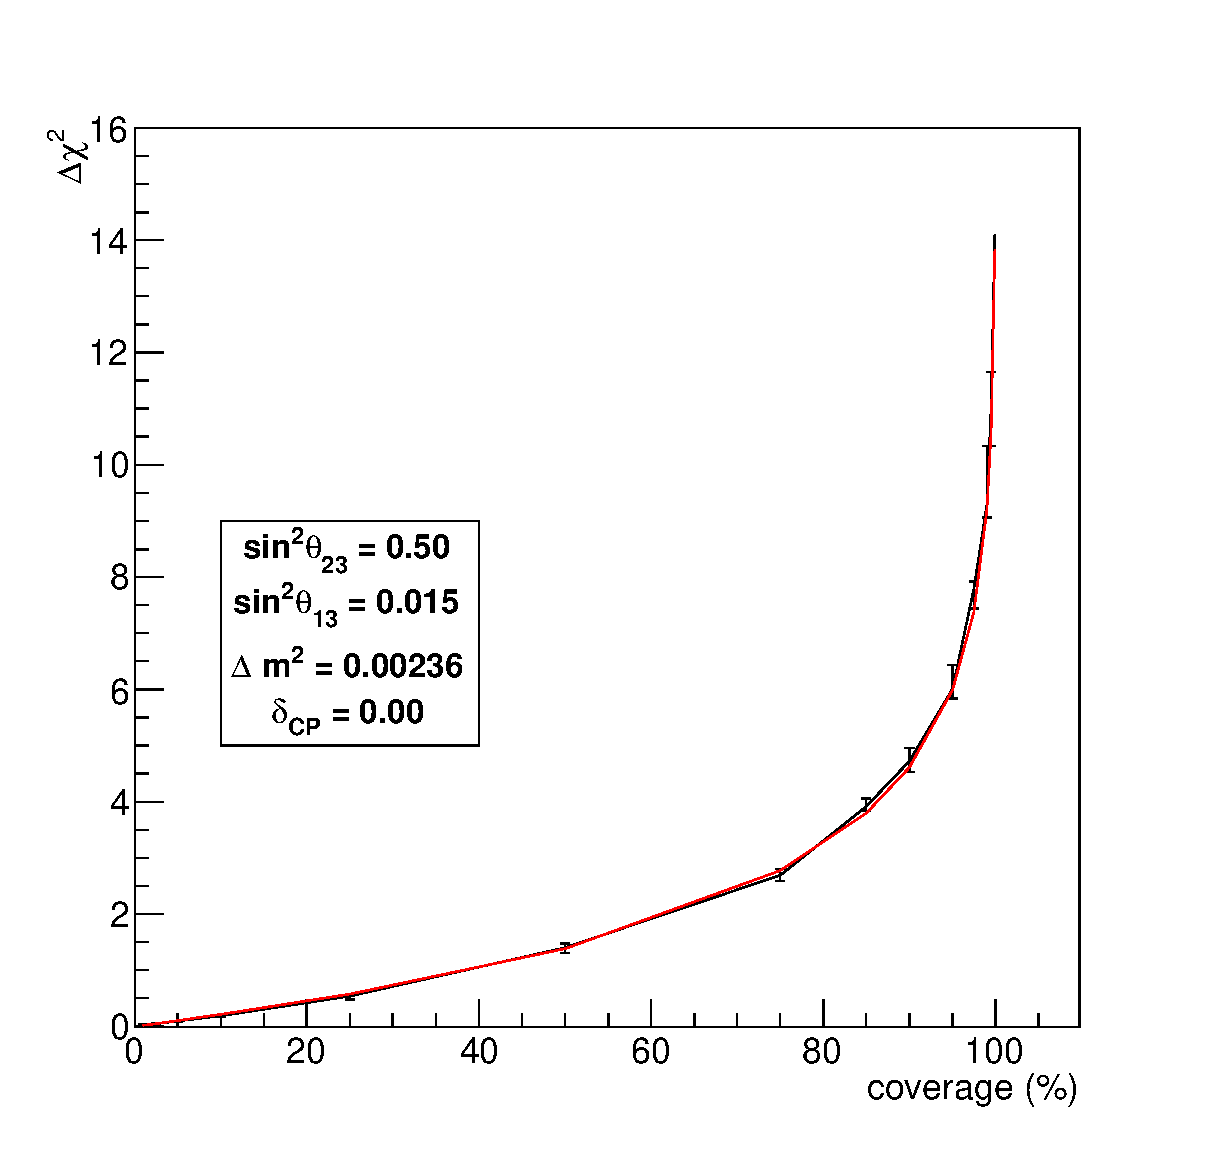
\includegraphics[width=14pc]{./images/appendix/coverage/coverage_study_2D_theta13_dm23sq_3.eps}
\center
\caption {
  Distribution of $\Delta\chi^{2}$ vs coverage in the ($sin^{2}\theta_{13}$,$|\Delta m^{2}|$) parameter space
  from 1k toy MC experiments generated with the Run 1+2+3 POT
  with statistical fluctuations at the oscillation point indicated in the legend.
}
\label{fig:cov_2D_theta13_dm23sq_3}
\end{minipage}
\hspace{0.03\linewidth}
\begin{minipage}[t]{0.46\linewidth}
\center
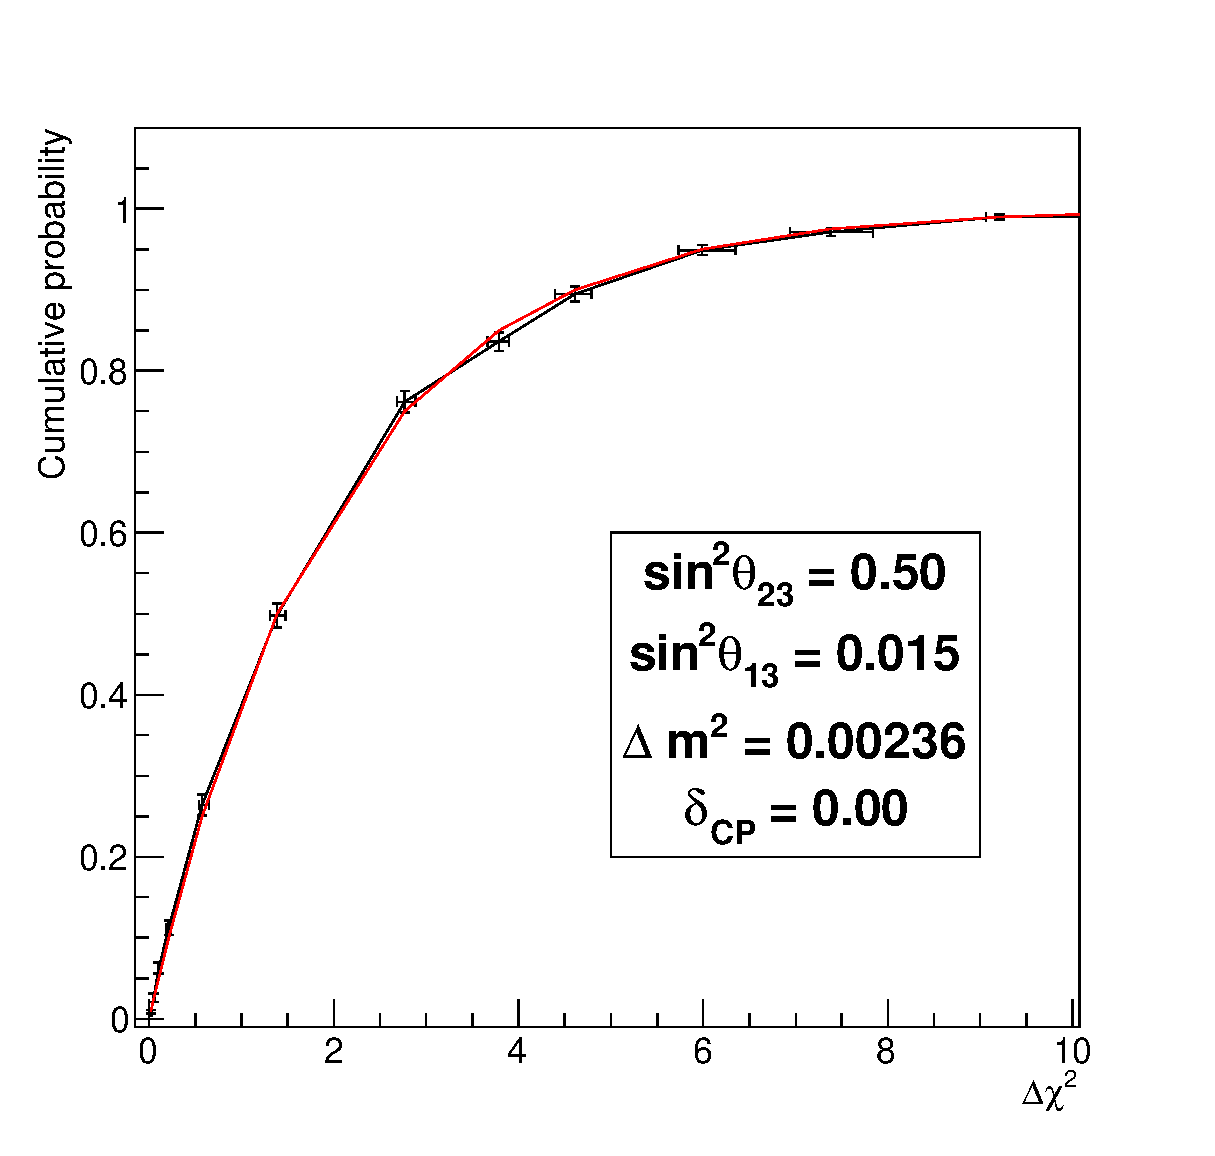
\includegraphics[width=14pc]{./images/appendix/coverage/coverage_study_2D_stats_theta13_dmsq_new_3.eps}
\center
\caption {
  Distribution of cumulative probability vs $\Delta\chi^{2}$ in the ($sin^{2}\theta_{13}$,$|\Delta m^{2}|$) parameter space
  from 1k toy MC experiments generated with the Run 1+2+3 POT
  with statistical fluctuations at the oscillation point indicated in the legend.
}
\label{fig:prob_2D_theta13_dm23sq_3}
\end{minipage}
\vfill
\vspace*{0.7cm}
\begin{minipage}[t]{0.46\linewidth}
\center
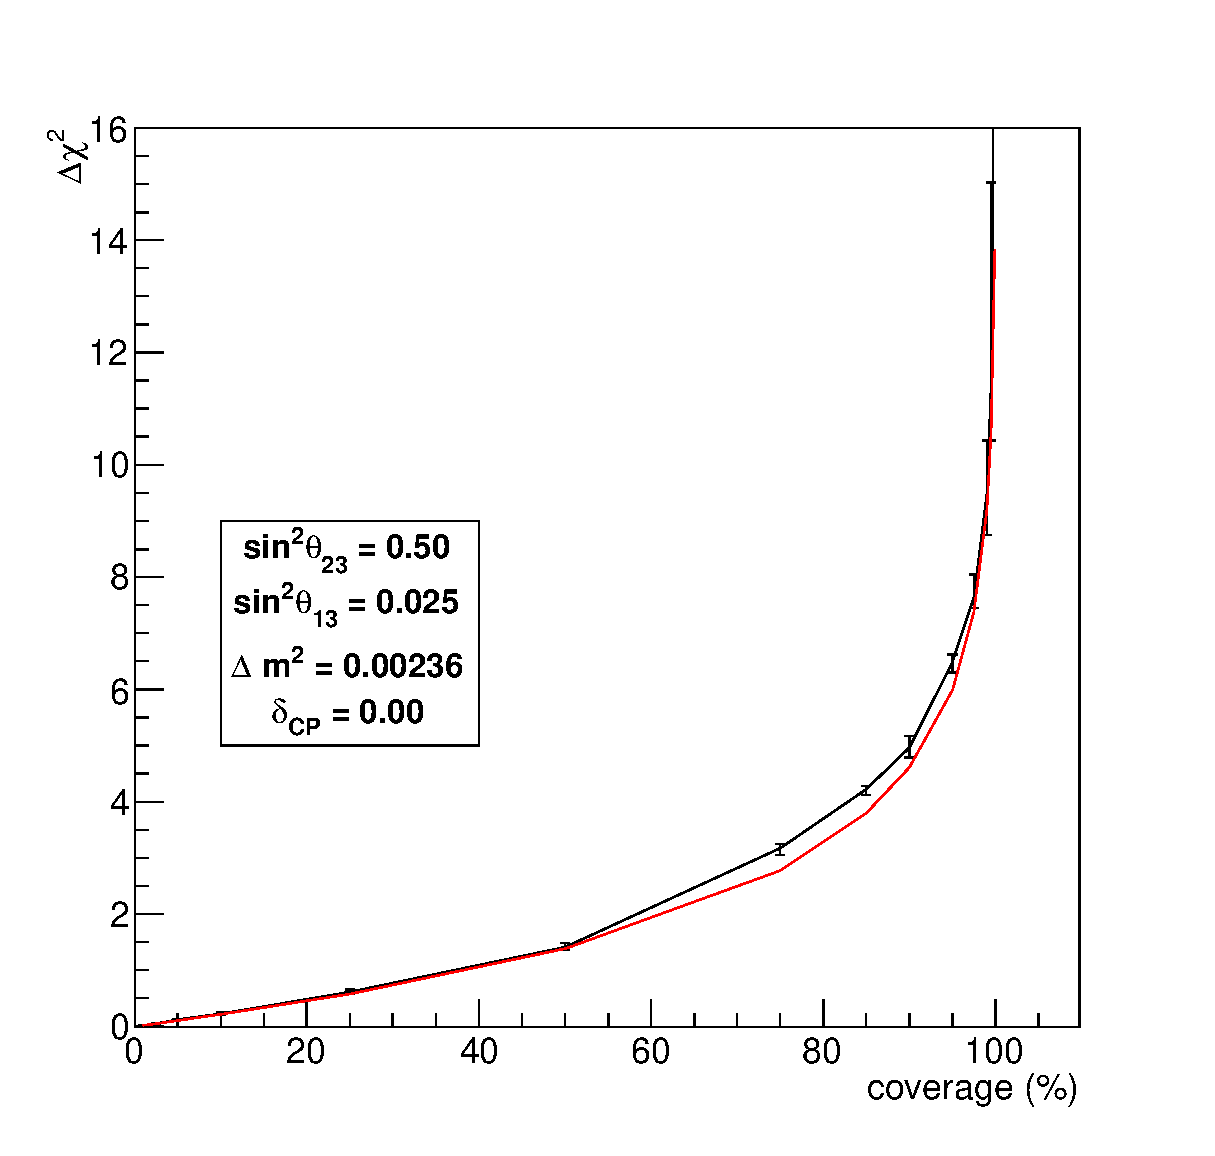
\includegraphics[width=14pc]{./images/appendix/coverage/coverage_study_2D_theta13_dm23sq_4.eps}
\center
\caption {
  Distribution of $\Delta\chi^{2}$ vs coverage in the ($sin^{2}\theta_{13}$,$|\Delta m^{2}|$) parameter space
  from 1k toy MC experiments generated with the Run 1+2+3 POT
  with statistical fluctuations at the oscillation point indicated in the legend.
}
\label{fig:cov_2D_theta13_dm23sq_4}
\end{minipage}
\hspace{0.03\linewidth}
\begin{minipage}[t]{0.46\linewidth}
\center
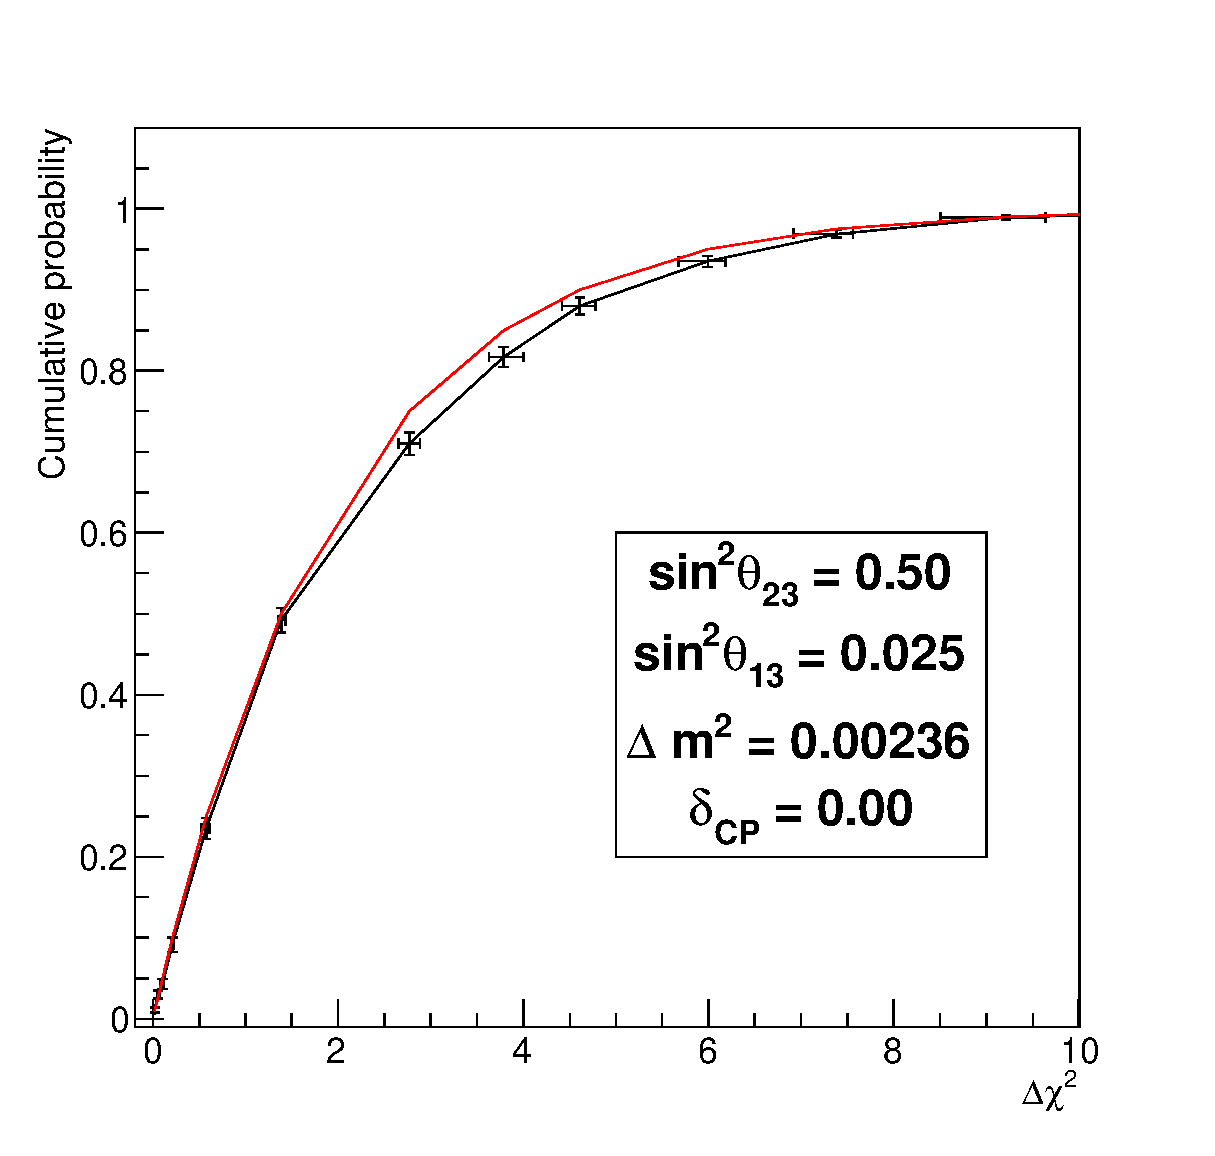
\includegraphics[width=14pc]{./images/appendix/coverage/coverage_study_2D_stats_theta13_dmsq_new_4.eps}
\center
\caption {
  Distribution of cumulative probability vs $\Delta\chi^{2}$ in the ($sin^{2}\theta_{13}$,$|\Delta m^{2}|$) parameter space
  from 1k toy MC experiments generated with the Run 1+2+3 POT
  with statistical fluctuations at the oscillation point indicated in the legend.
}
\label{fig:prob_2D_theta13_dm23sq_4}
\end{minipage}
\vfill
\vspace*{0.7cm}
\begin{minipage}[t]{0.46\linewidth}
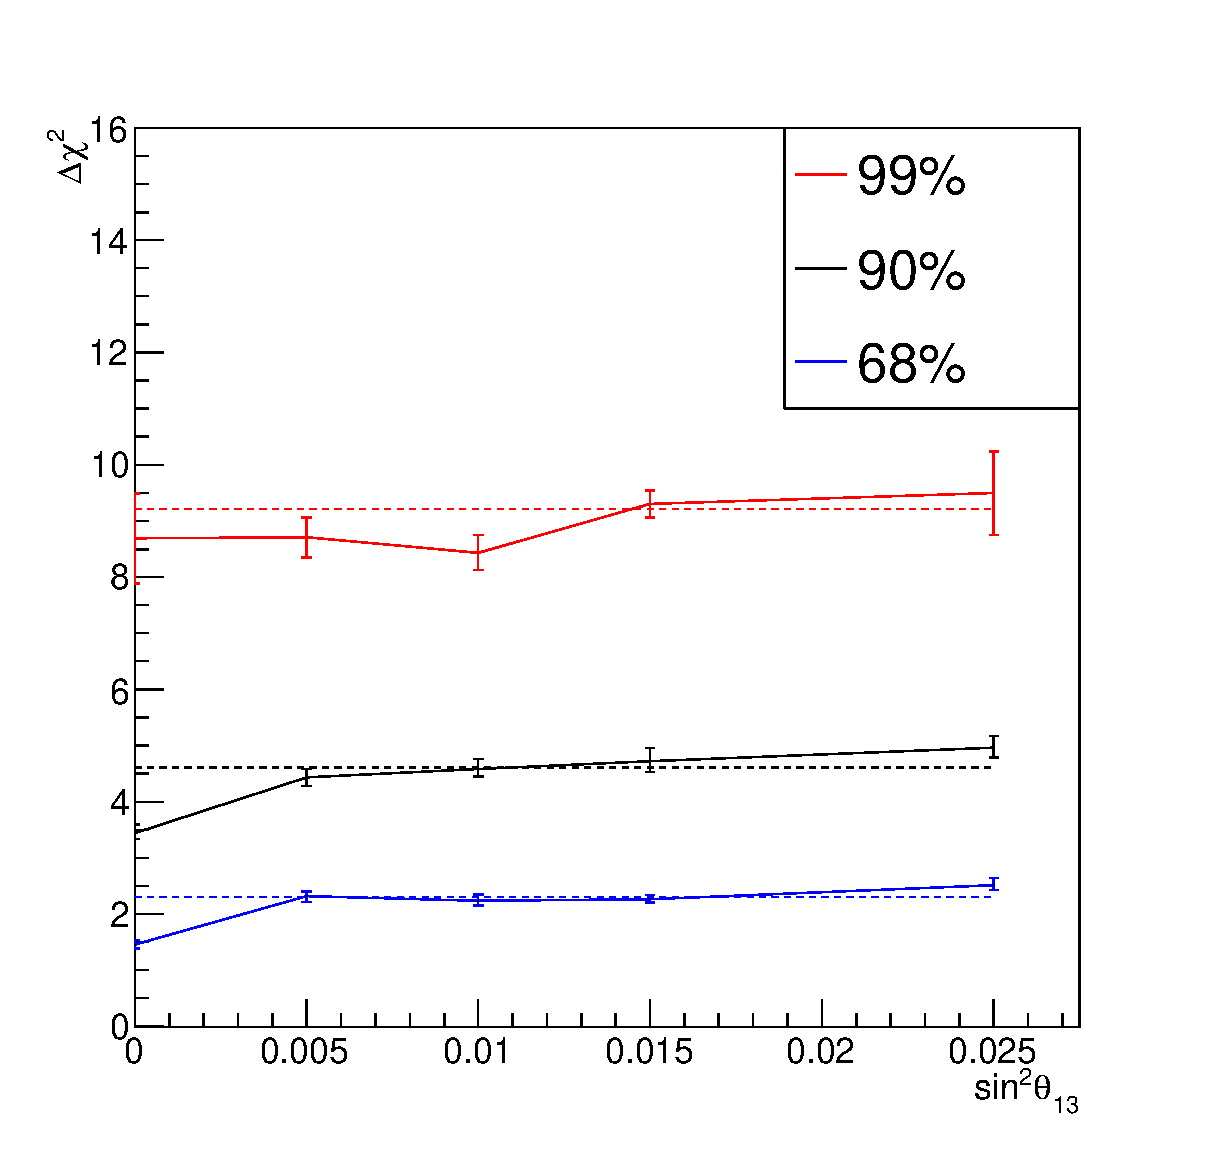
\includegraphics[width=14pc]{./images/appendix/coverage/coverage_study_2D_theta13_dm23sq_all.eps}
\center
\caption {
   Summary of figures \ref{fig:cov_2D_theta13_dm23sq_0}-\ref{fig:cov_2D_theta13_dm23sq_4}
showing the value of $\Delta\chi^{2}$ at 99\%, 90\% and 68\% confidence intervals vs the value of $sin^{2}\theta_{13}$.
Horizontal dashed lines show the canonical $\Delta\chi^{2}$ value for 2 degrees of freedom.
	}
\label{fig:cov_2D_theta13_dm23sq_all}
\end{minipage}
\hspace{0.03\linewidth}
\begin{minipage}[t]{0.46\linewidth}
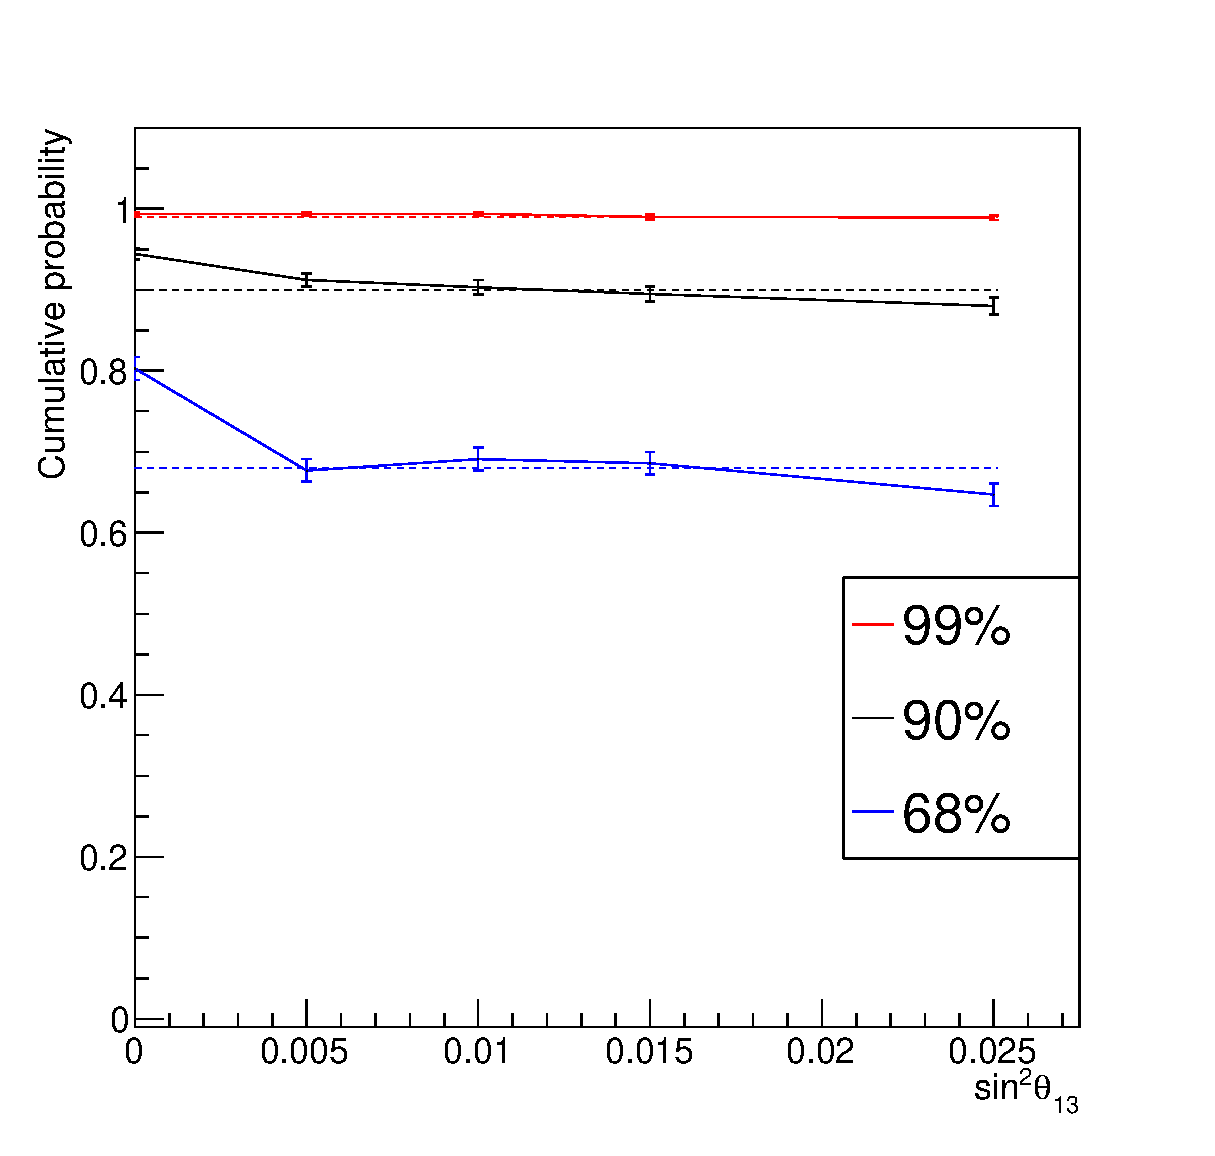
\includegraphics[width=14pc]{./images/appendix/coverage/coverage_study_2D_stats_theta13_dmsq_new_all.eps}
\center
\caption {
   Summary of figures \ref{fig:prob_2D_theta13_dm23sq_0}-\ref{fig:prob_2D_theta13_dm23sq_4}
showing the value of cumulative probability for $\Delta\chi^{2}=9.21$ (canonical value for 99\%), $\Delta\chi^{2}=4.61$ (canonical value for 90\%) and $\Delta\chi^{2}=2.30$ (canonical value for 68\%) vs the value of $sin^{2}\theta_{13}$.
	}
\label{fig:cov_2D_theta13_dm23sq_all}
\end{minipage}
\end{figure*}
\end{center}


%% FIGURES FOR 2D theta13-dmsq

\begin{center}
\begin{figure*}[htb]
\begin{minipage}[t]{0.46\linewidth}
\center
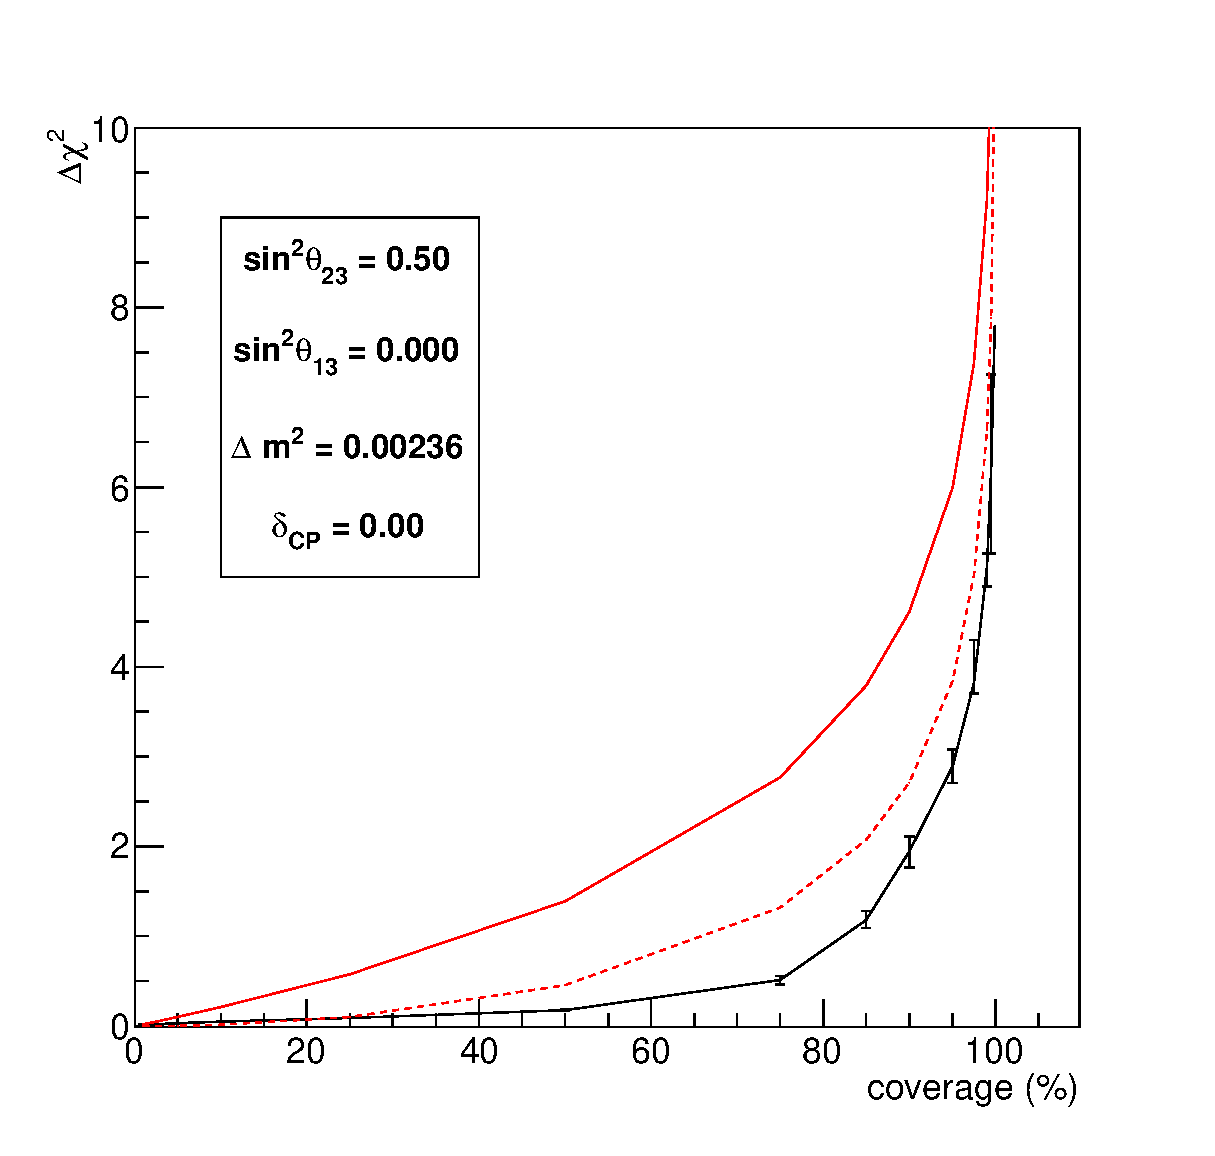
\includegraphics[width=14pc]{./images/appendix/coverage/coverage_study_2D_theta13_deltacp_0.eps}
\center
\caption {
  Distribution of $\Delta\chi^{2}$ vs coverage in the ($sin^{2}\theta_{13}$,$\delta_{CP}$) parameter space
  from 1k toy MC experiments generated with the Run 1+2+3 POT
  with statistical fluctuations at the oscillation point indicated in the legend.
 The solid red line shows the canonical $\Delta\chi^{2}$ pdf for 2 degrees of freedom and the dashed red line shows the canonical $\Delta\chi^{2}$ pdf for 1 degree of freedom.
}
\label{fig:cov_2D_theta13_deltacp_0}
\end{minipage}
\hspace{0.03\linewidth}
\begin{minipage}[t]{0.46\linewidth}
\center
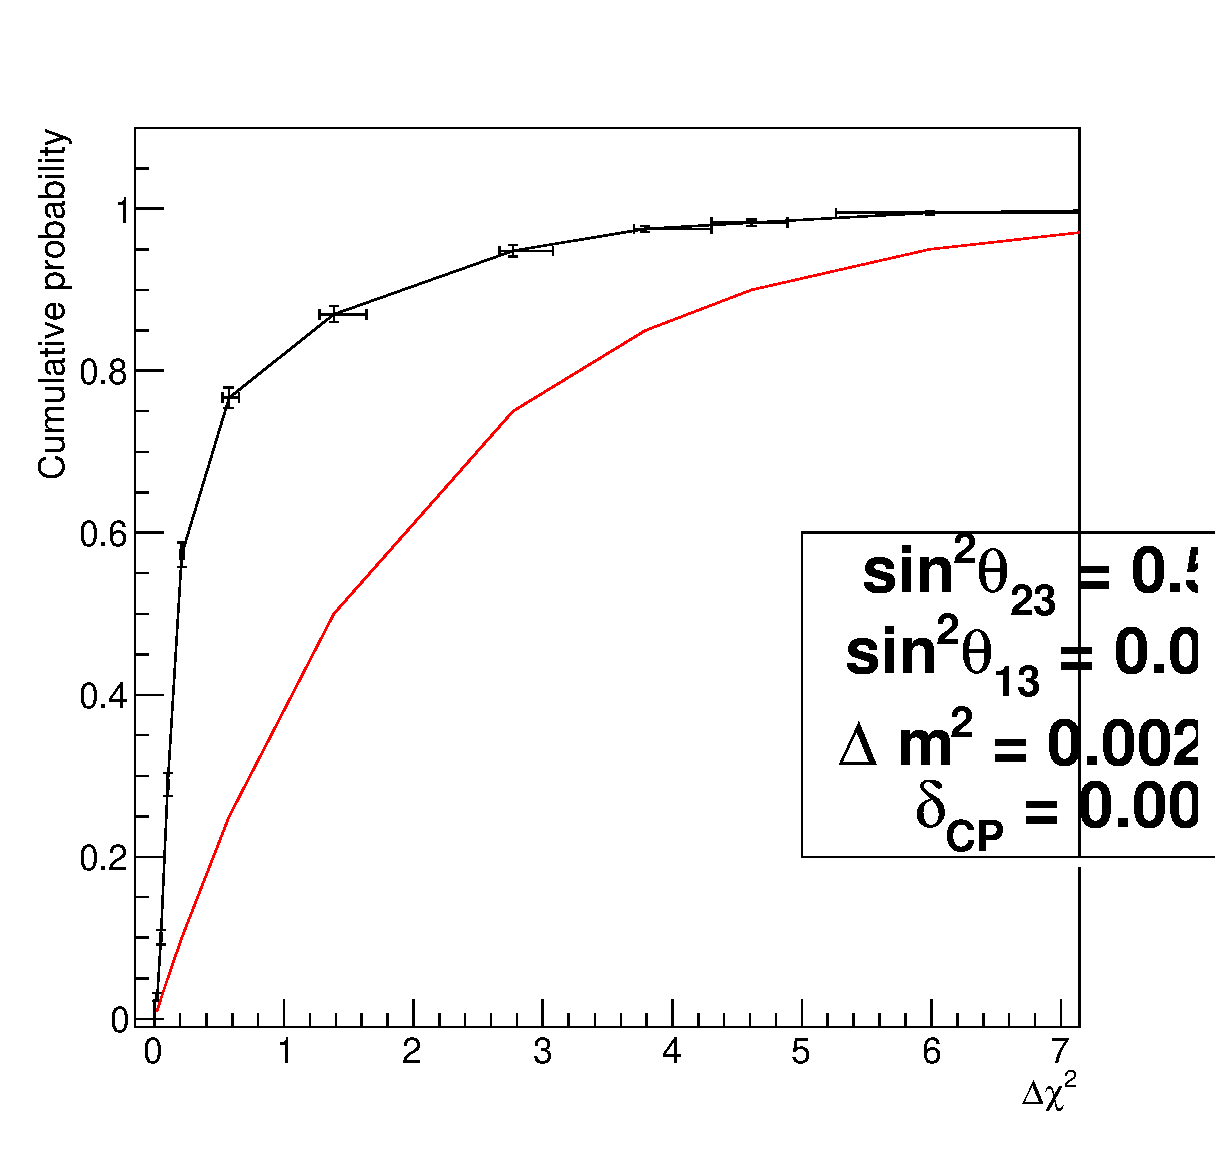
\includegraphics[width=14pc]{./images/appendix/coverage/coverage_study_2D_stats_theta13_deltacp_new_0.eps}
\center
\caption {
  Distribution of cumulative probability vs $\Delta\chi^{2}$ in the ($sin^{2}\theta_{13}$,$\delta_{CP}$) parameter space
  from 1k toy MC experiments generated with the Run 1+2+3 POT
  with statistical fluctuations at the oscillation point indicated in the legend.
}
\label{fig:prob_2D_theta13_deltacp_0}
\end{minipage}
\vfill
\vspace*{0.7cm}
\begin{minipage}[t]{0.46\linewidth}
\center
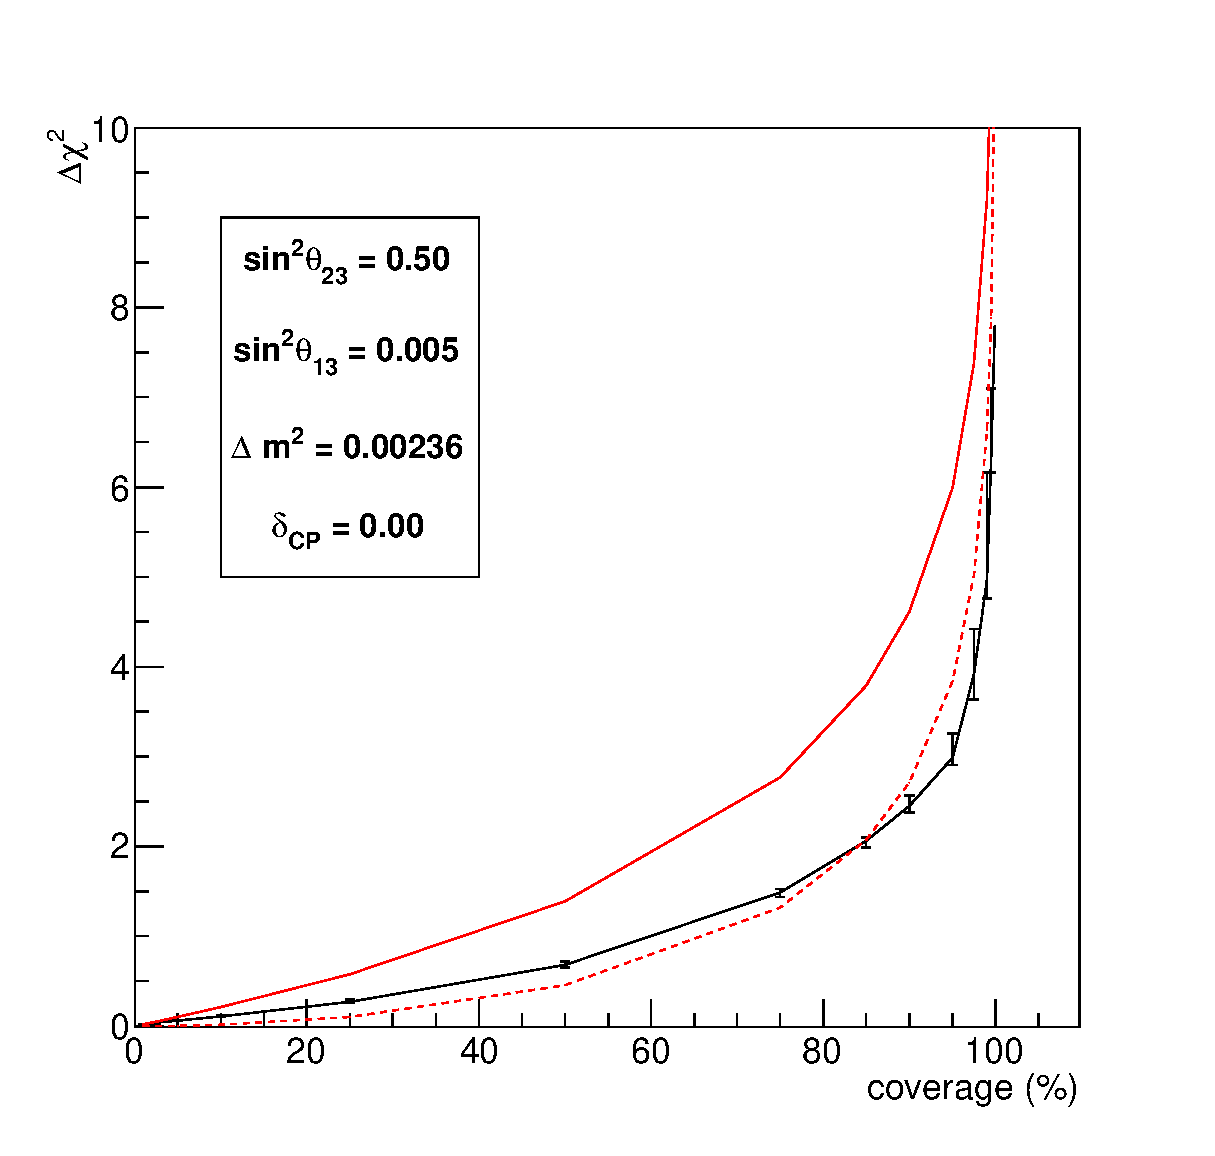
\includegraphics[width=14pc]{./images/appendix/coverage/coverage_study_2D_theta13_deltacp_1.eps}
\center
\caption {
  Distribution of $\Delta\chi^{2}$ vs coverage in the ($sin^{2}\theta_{13}$,$\delta_{CP}$) parameter space
  from 1k toy MC experiments generated with the Run 1+2+3 POT
  with statistical fluctuations at the oscillation point indicated in the legend.
 The solid red line shows the canonical $\Delta\chi^{2}$ pdf for 2 degrees of freedom and the dashed red line shows the canonical $\Delta\chi^{2}$ pdf for 1 degree of freedom.
}
\label{fig:cov_2D_theta13_deltacp_1}
\end{minipage}
\hspace{0.03\linewidth}
\begin{minipage}[t]{0.46\linewidth}
\center
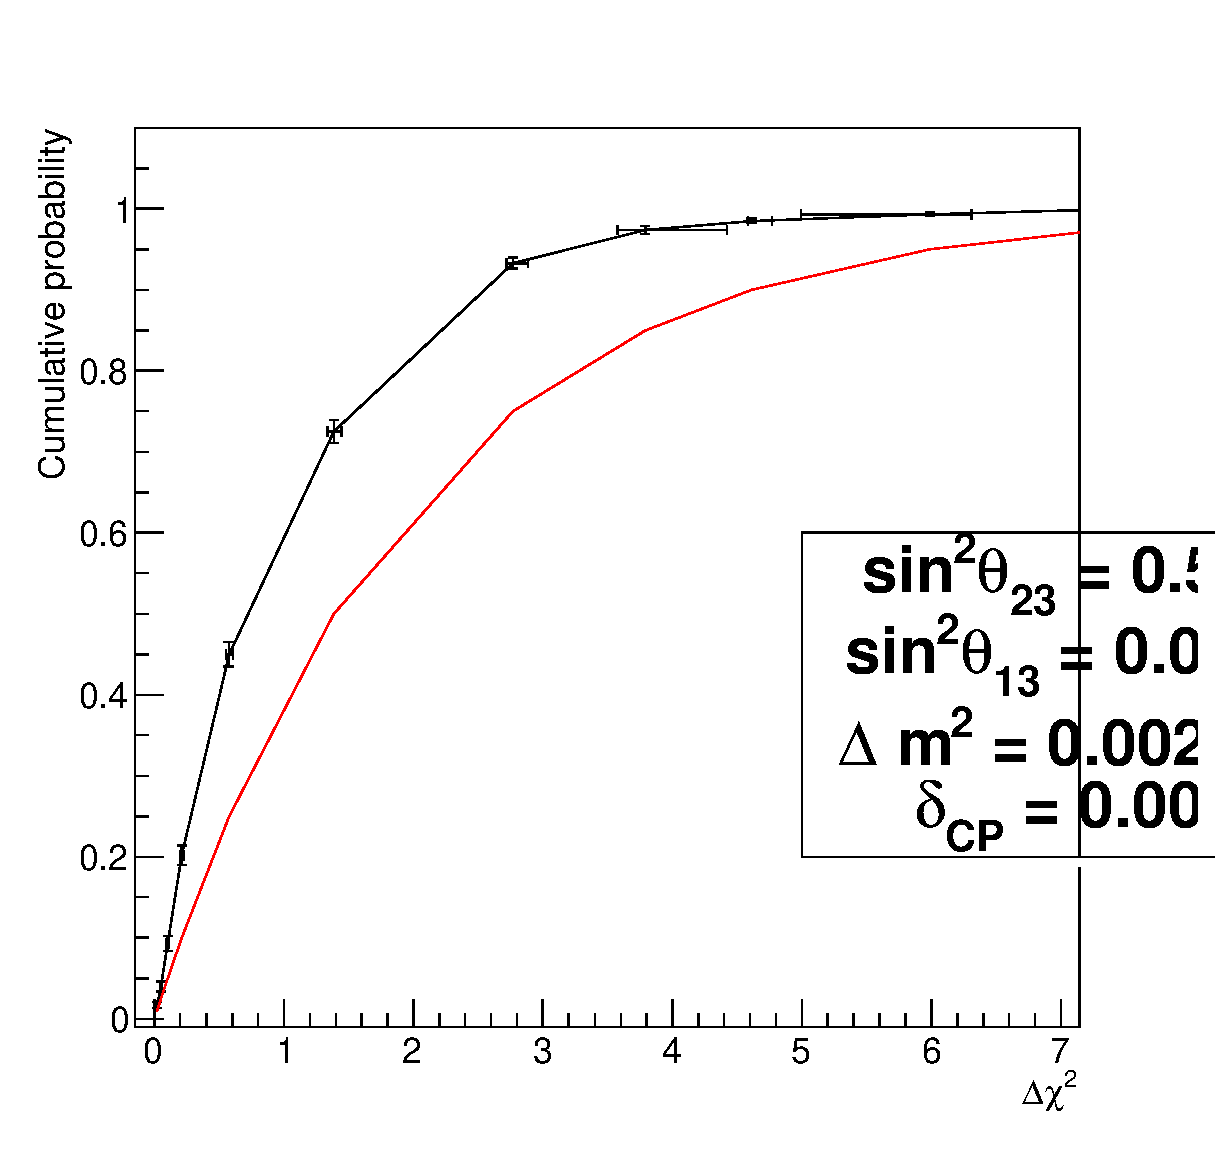
\includegraphics[width=14pc]{./images/appendix/coverage/coverage_study_2D_stats_theta13_deltacp_new_1.eps}
\center
\caption {
  Distribution of cumulative probability vs $\Delta\chi^{2}$ in the ($sin^{2}\theta_{13}$,$\delta_{CP}$) parameter space
  from 1k toy MC experiments generated with the Run 1+2+3 POT
  with statistical fluctuations at the oscillation point indicated in the legend.
}
\label{fig:prob_2D_theta13_deltacp_1}
\end{minipage}
\vfill
\vspace*{0.7cm}
\begin{minipage}[t]{0.46\linewidth}
\center
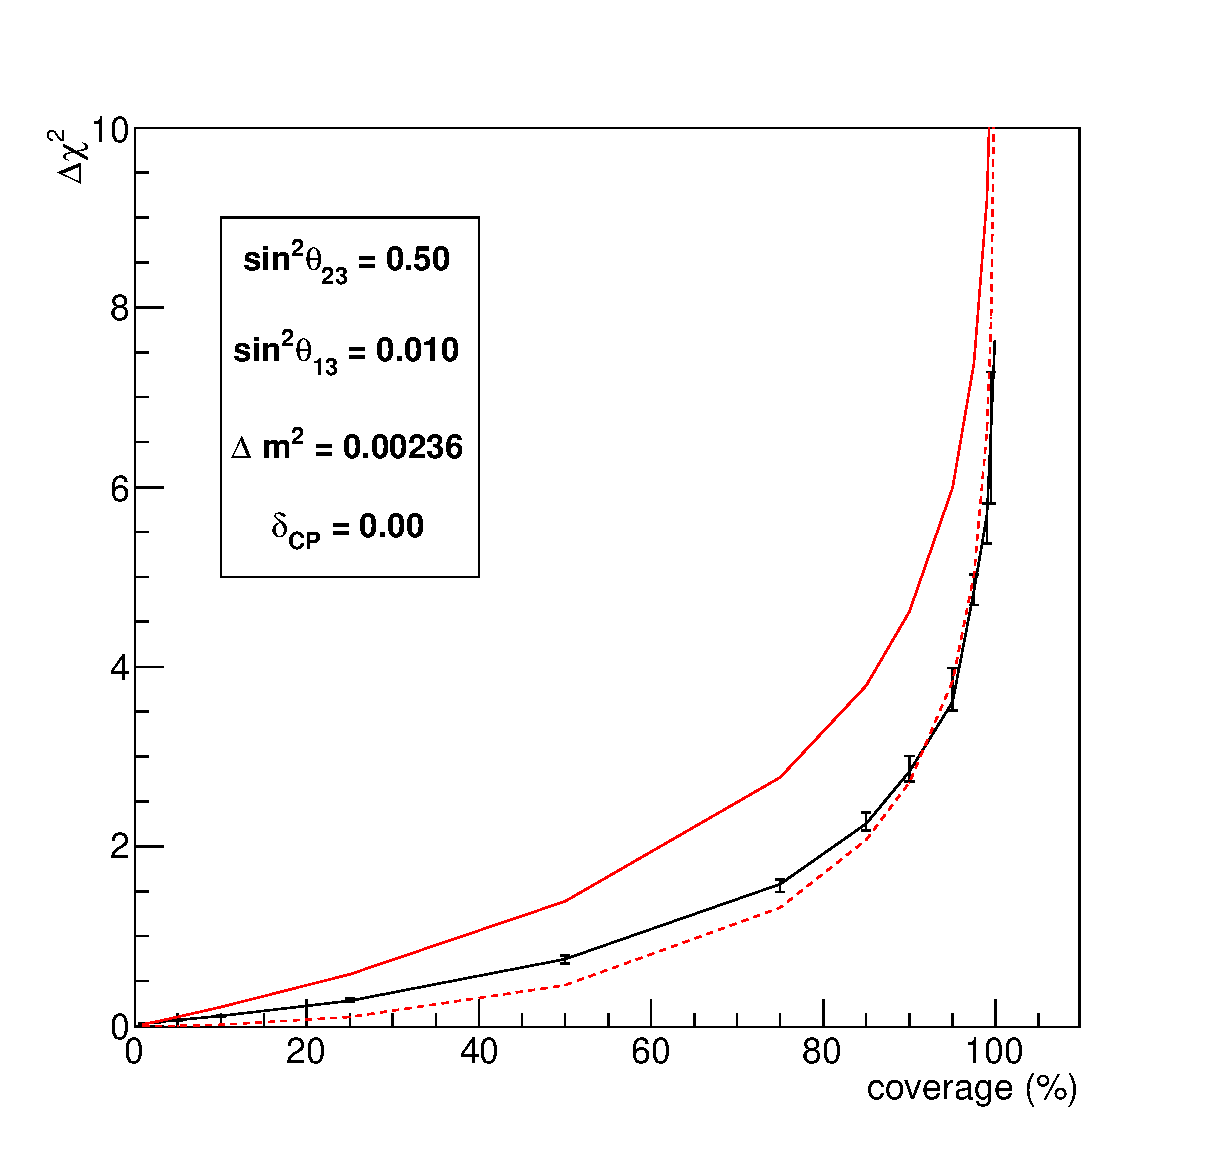
\includegraphics[width=14pc]{./images/appendix/coverage/coverage_study_2D_theta13_deltacp_2.eps}
\center
\caption {
  Distribution of $\Delta\chi^{2}$ vs coverage in the ($sin^{2}\theta_{13}$,$\delta_{CP}$) parameter space
  from 1k toy MC experiments generated with the Run 1+2+3 POT
  with statistical fluctuations at the oscillation point indicated in the legend.
 The solid red line shows the canonical $\Delta\chi^{2}$ pdf for 2 degrees of freedom and the dashed red line shows the canonical $\Delta\chi^{2}$ pdf for 1 degree of freedom.
}
\label{fig:cov_2D_theta13_deltacp_2}
\end{minipage}
\hspace{0.03\linewidth}
\begin{minipage}[t]{0.46\linewidth}
\center
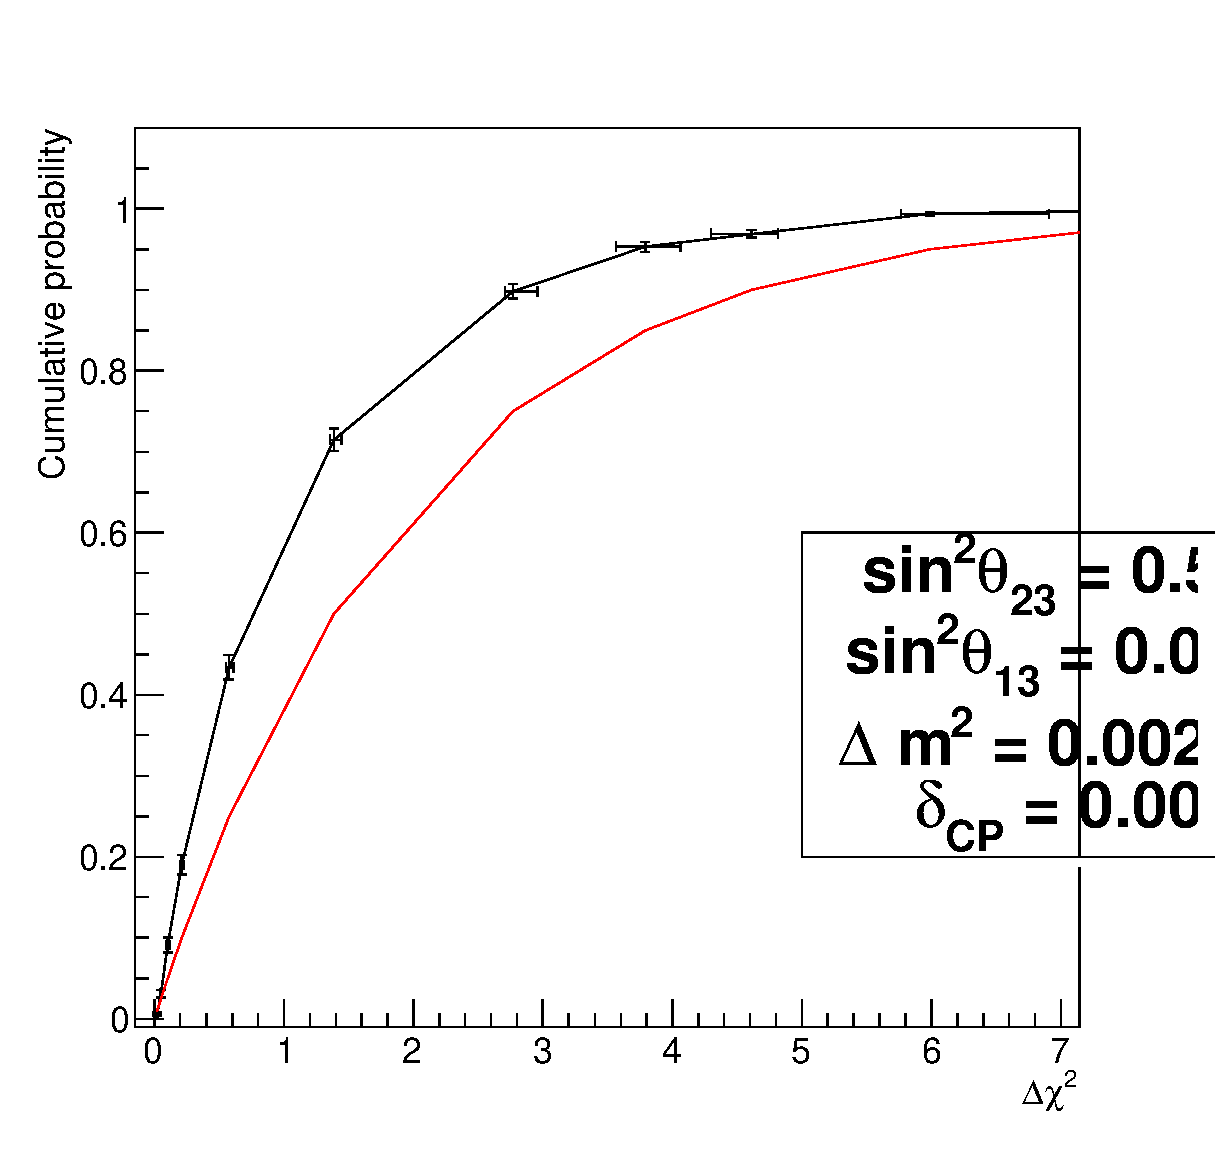
\includegraphics[width=14pc]{./images/appendix/coverage/coverage_study_2D_stats_theta13_deltacp_new_2.eps}
\center
\caption {
  Distribution of cumulative probability vs $\Delta\chi^{2}$ in the ($sin^{2}\theta_{13}$,$\delta_{CP}$) parameter space
  from 1k toy MC experiments generated with the Run 1+2+3 POT
  with statistical fluctuations at the oscillation point indicated in the legend.
}
\label{fig:prob_2D_theta13_deltacp_2}
\end{minipage}
\end{figure*}
\end{center}

\begin{center}
\begin{figure*}[htb]
\begin{minipage}[t]{0.46\linewidth}
\center
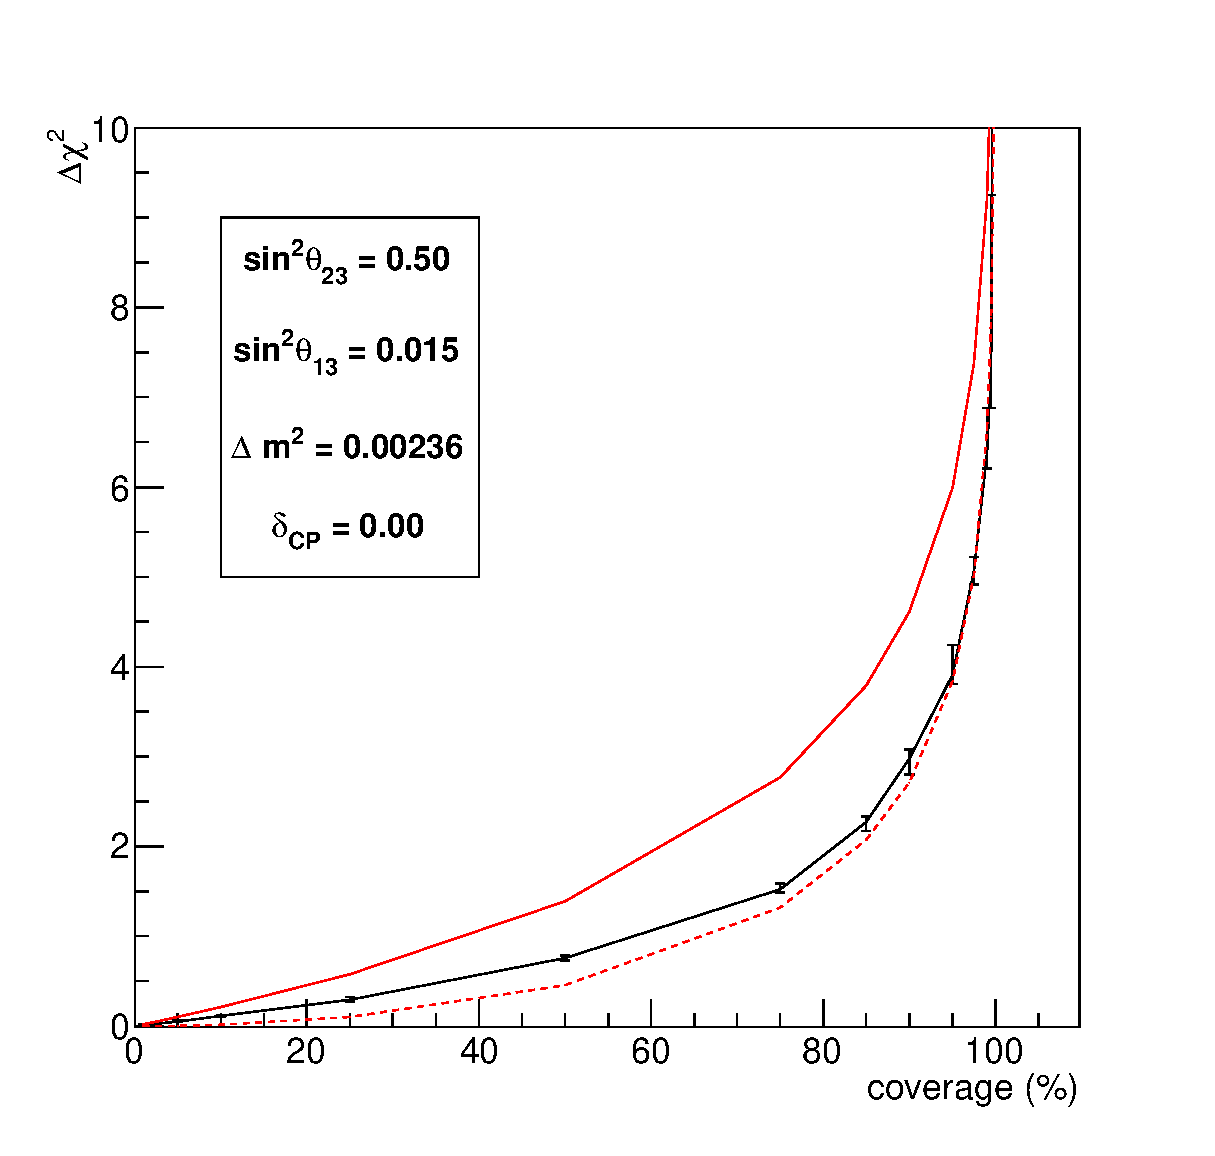
\includegraphics[width=14pc]{./images/appendix/coverage/coverage_study_2D_theta13_deltacp_3.eps}
\center
\caption {
  Distribution of $\Delta\chi^{2}$ vs coverage in the ($sin^{2}\theta_{13}$,$\delta_{CP}$) parameter space
  from 1k toy MC experiments generated with the Run 1+2+3 POT
  with statistical fluctuations at the oscillation point indicated in the legend.
 The solid red line shows the canonical $\Delta\chi^{2}$ pdf for 2 degrees of freedom and the dashed red line shows the canonical $\Delta\chi^{2}$ pdf for 1 degree of freedom.
}
\label{fig:cov_2D_theta13_deltacp_3}
\end{minipage}
\hspace{0.03\linewidth}
\begin{minipage}[t]{0.46\linewidth}
\center
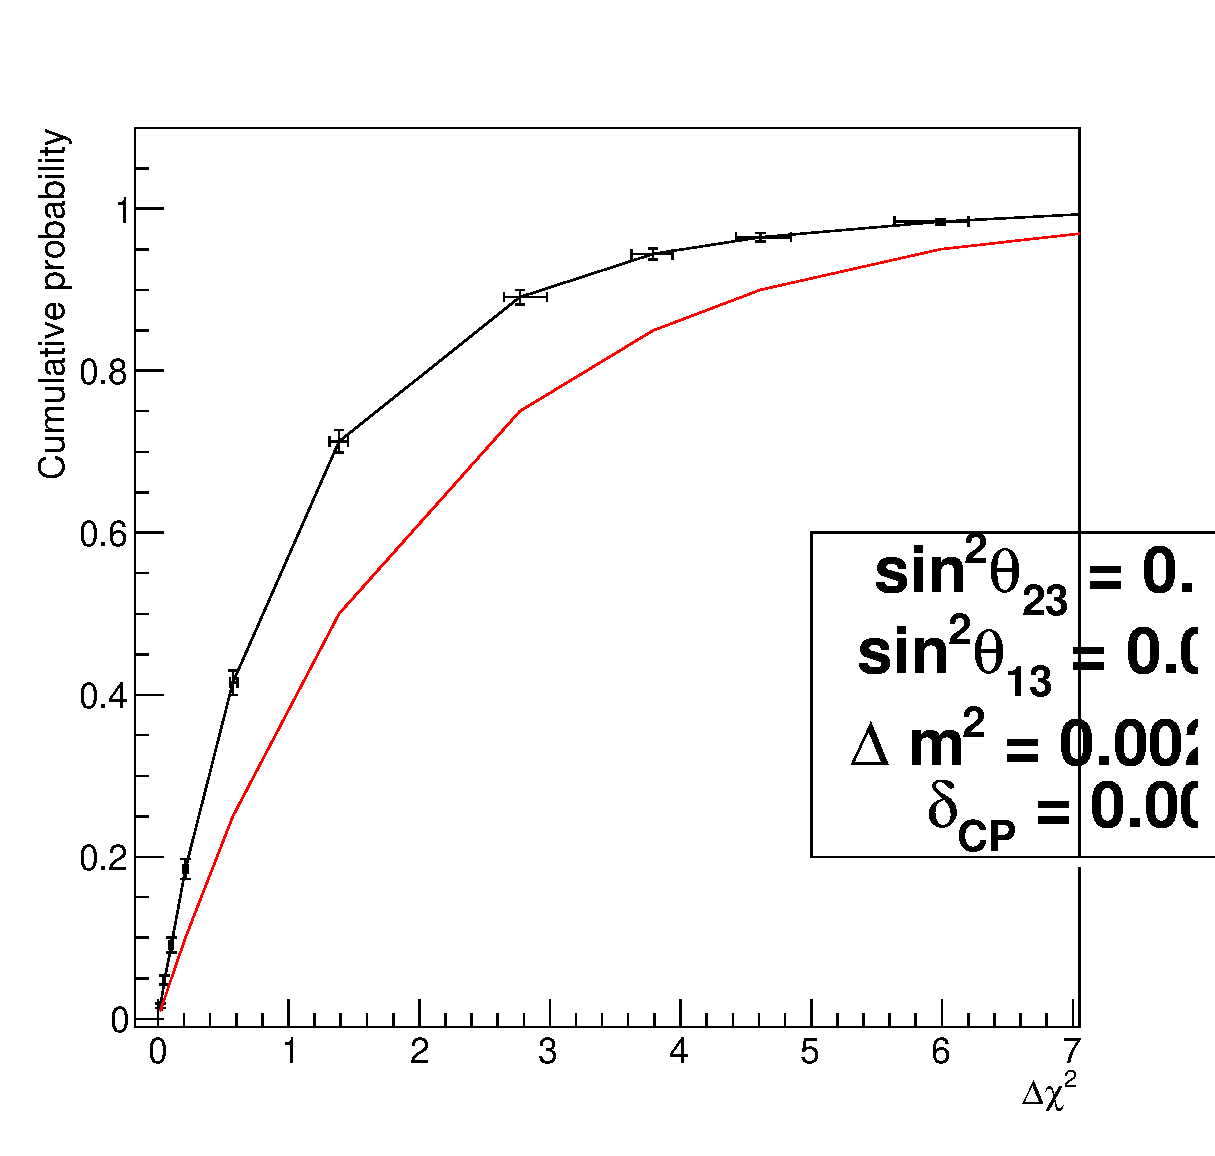
\includegraphics[width=14pc]{./images/appendix/coverage/coverage_study_2D_stats_theta13_deltacp_new_3.eps}
\center
\caption {
  Distribution of cumulative probability vs $\Delta\chi^{2}$ in the ($sin^{2}\theta_{13}$,$\delta_{CP}$) parameter space
  from 1k toy MC experiments generated with the Run 1+2+3 POT
  with statistical fluctuations at the oscillation point indicated in the legend.
}
\label{fig:prob_2D_theta13_deltacp_3}
\end{minipage}
\vfill
\vspace*{0.7cm}
\begin{minipage}[t]{0.46\linewidth}
\center
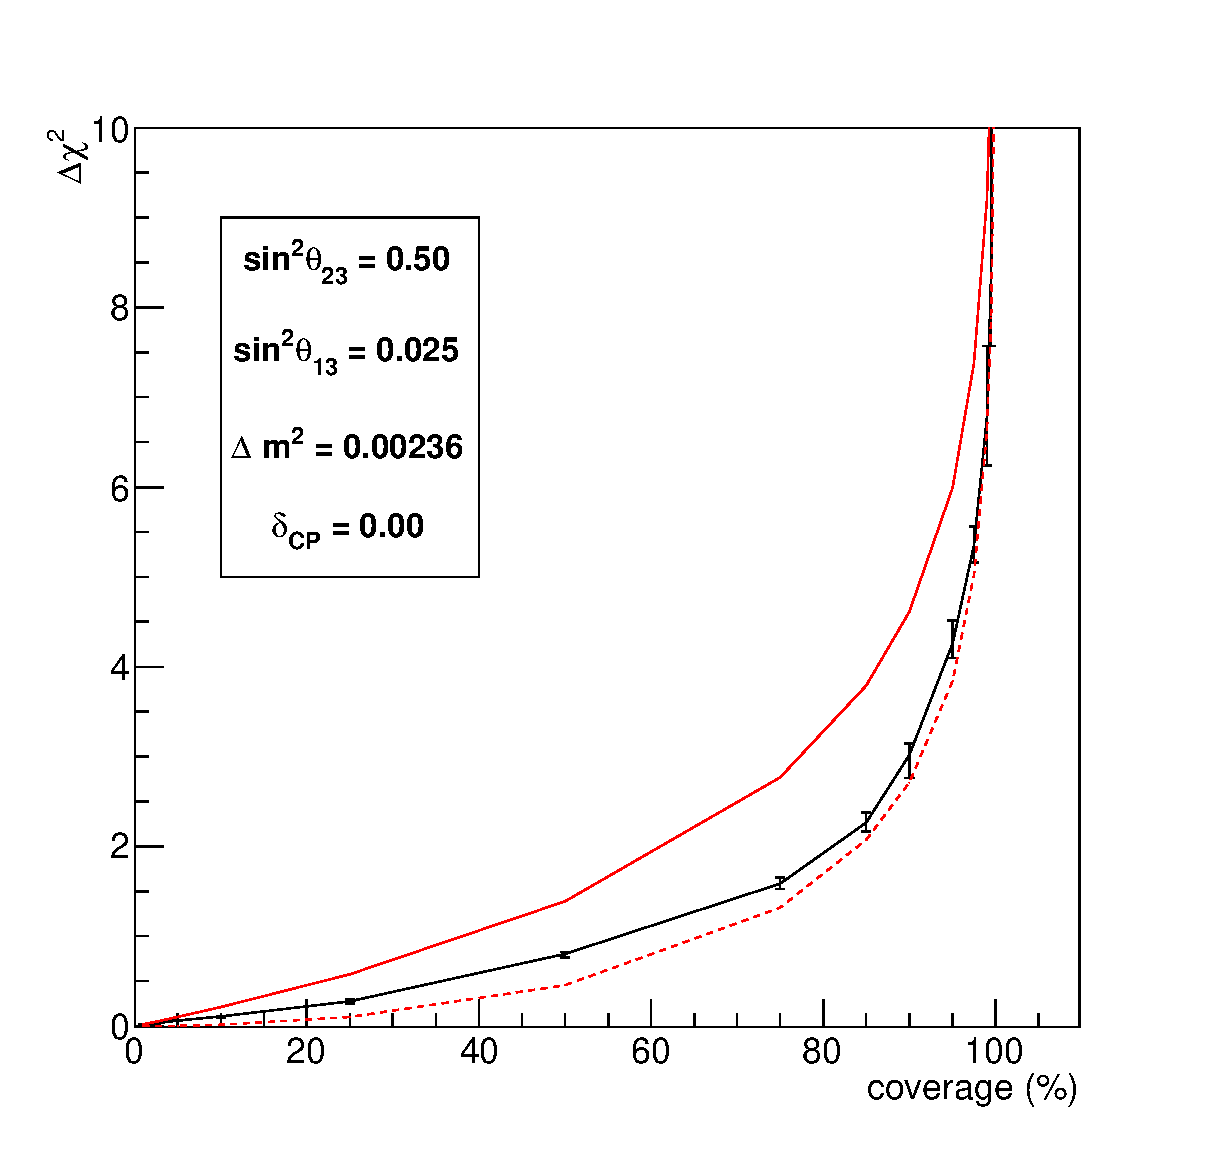
\includegraphics[width=14pc]{./images/appendix/coverage/coverage_study_2D_theta13_deltacp_4.eps}
\center
\caption {
  Distribution of $\Delta\chi^{2}$ vs coverage in the ($sin^{2}\theta_{13}$,$\delta_{CP}$) parameter space
  from 1k toy MC experiments generated with the Run 1+2+3 POT
  with statistical fluctuations at the oscillation point indicated in the legend.
 The solid red line shows the canonical $\Delta\chi^{2}$ pdf for 2 degrees of freedom and the dashed red line shows the canonical $\Delta\chi^{2}$ pdf for 1 degree of freedom.
}
\label{fig:cov_2D_theta13_deltacp_4}
\end{minipage}
\hspace{0.03\linewidth}
\begin{minipage}[t]{0.46\linewidth}
\center
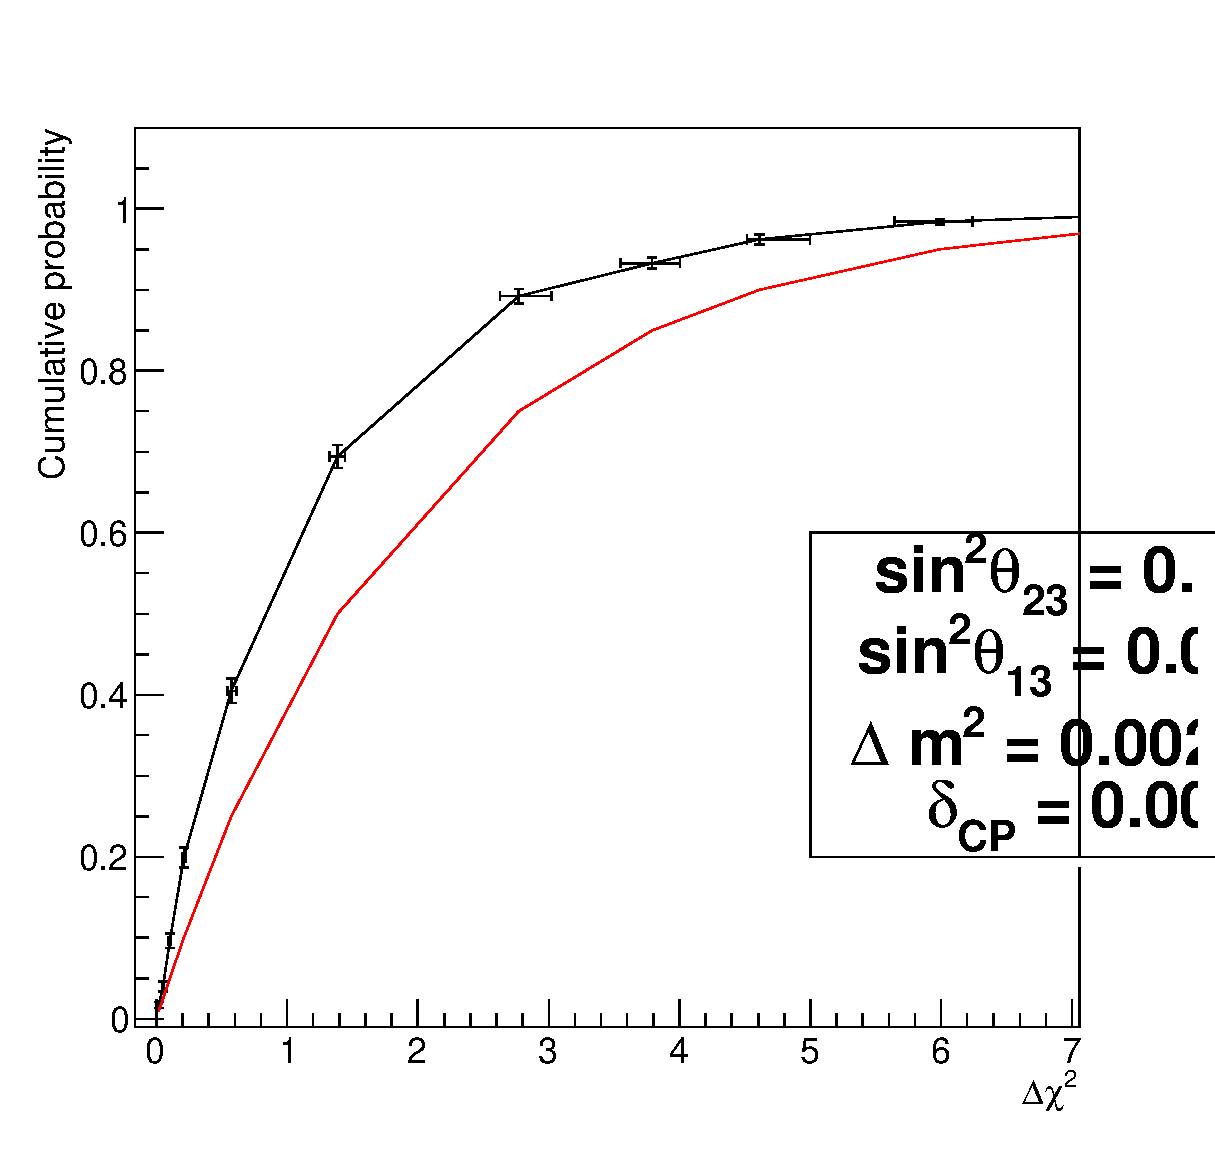
\includegraphics[width=14pc]{./images/appendix/coverage/coverage_study_2D_stats_theta13_deltacp_new_4.eps}
\center
\caption {
  Distribution of cumulative probability vs $\Delta\chi^{2}$ in the ($sin^{2}\theta_{13}$,$\delta_{CP}$) parameter space
  from 1k toy MC experiments generated with the Run 1+2+3 POT
  with statistical fluctuations at the oscillation point indicated in the legend.
}
\label{fig:prob_2D_theta13_deltacp_4}
\end{minipage}
\vfill
\vspace*{0.7cm}
\begin{minipage}[t]{0.46\linewidth}
\center
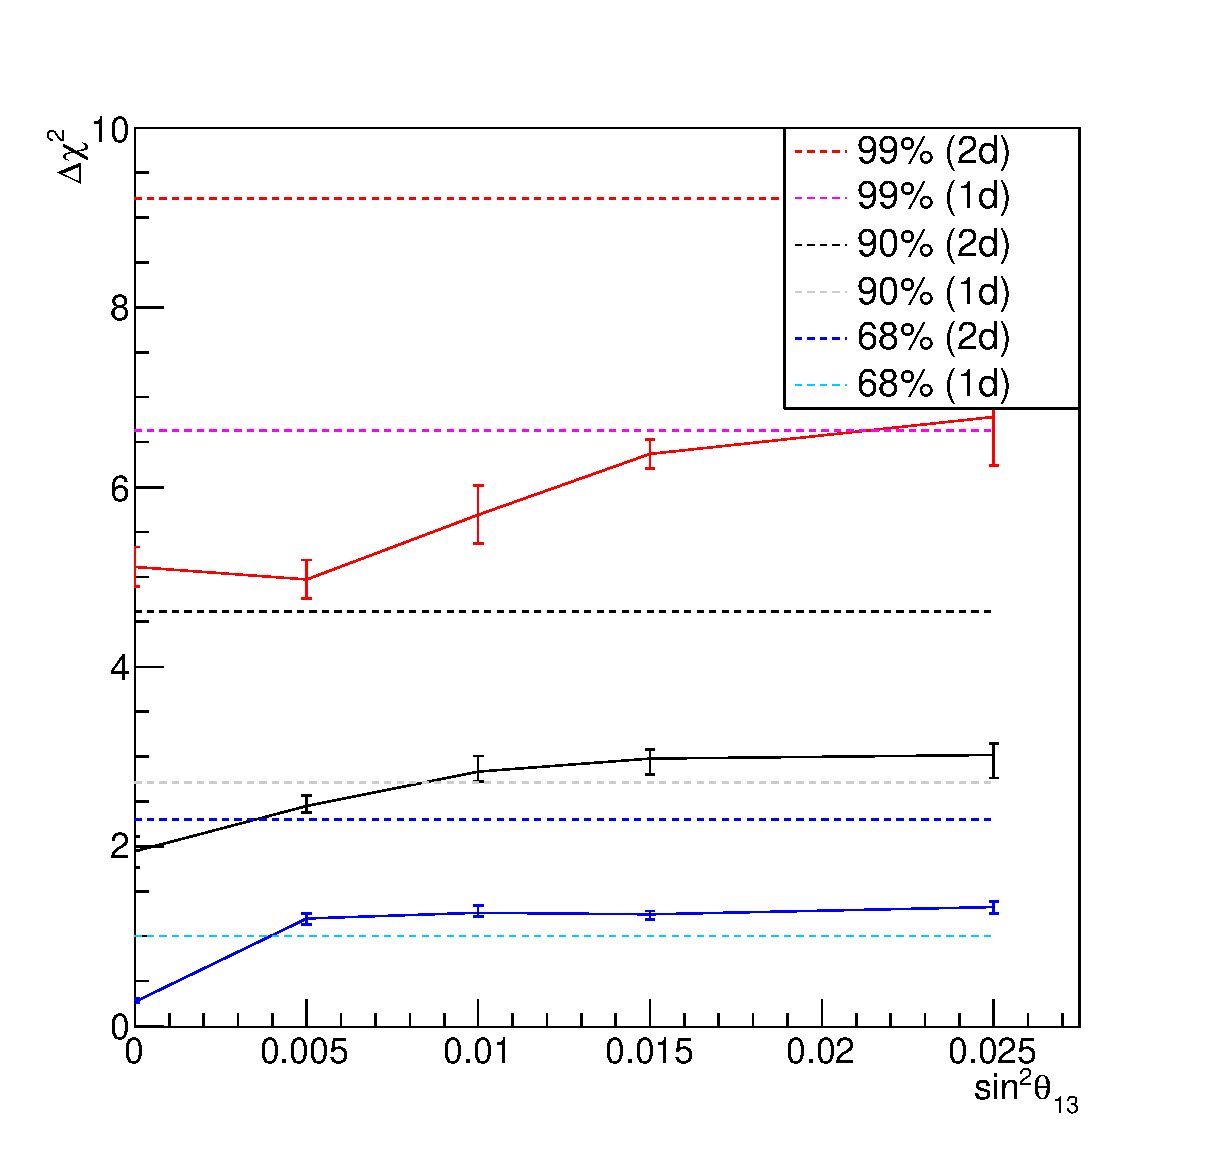
\includegraphics[width=14pc]{./images/appendix/coverage/coverage_study_2D_theta13_deltacp_all.eps}
\center
\caption {
   Summary of figures \ref{fig:cov_2D_theta13_deltacp_0}-\ref{fig:cov_2D_theta13_deltacp_4}
showing the value of $\Delta\chi^{2}$ at 99\%, 90\% and 68\% confidence intervals vs the value of $sin^{2}\theta_{13}$.
Horizontal dashed lines show the canonical $\Delta\chi^{2}$ value for 2 degrees of freedom and 1 degree of freedom (see legend).
	}
\label{fig:cov_2D_theta13_deltacp_all}
\end{minipage}
\hspace{0.03\linewidth}
\begin{minipage}[t]{0.46\linewidth}
\center
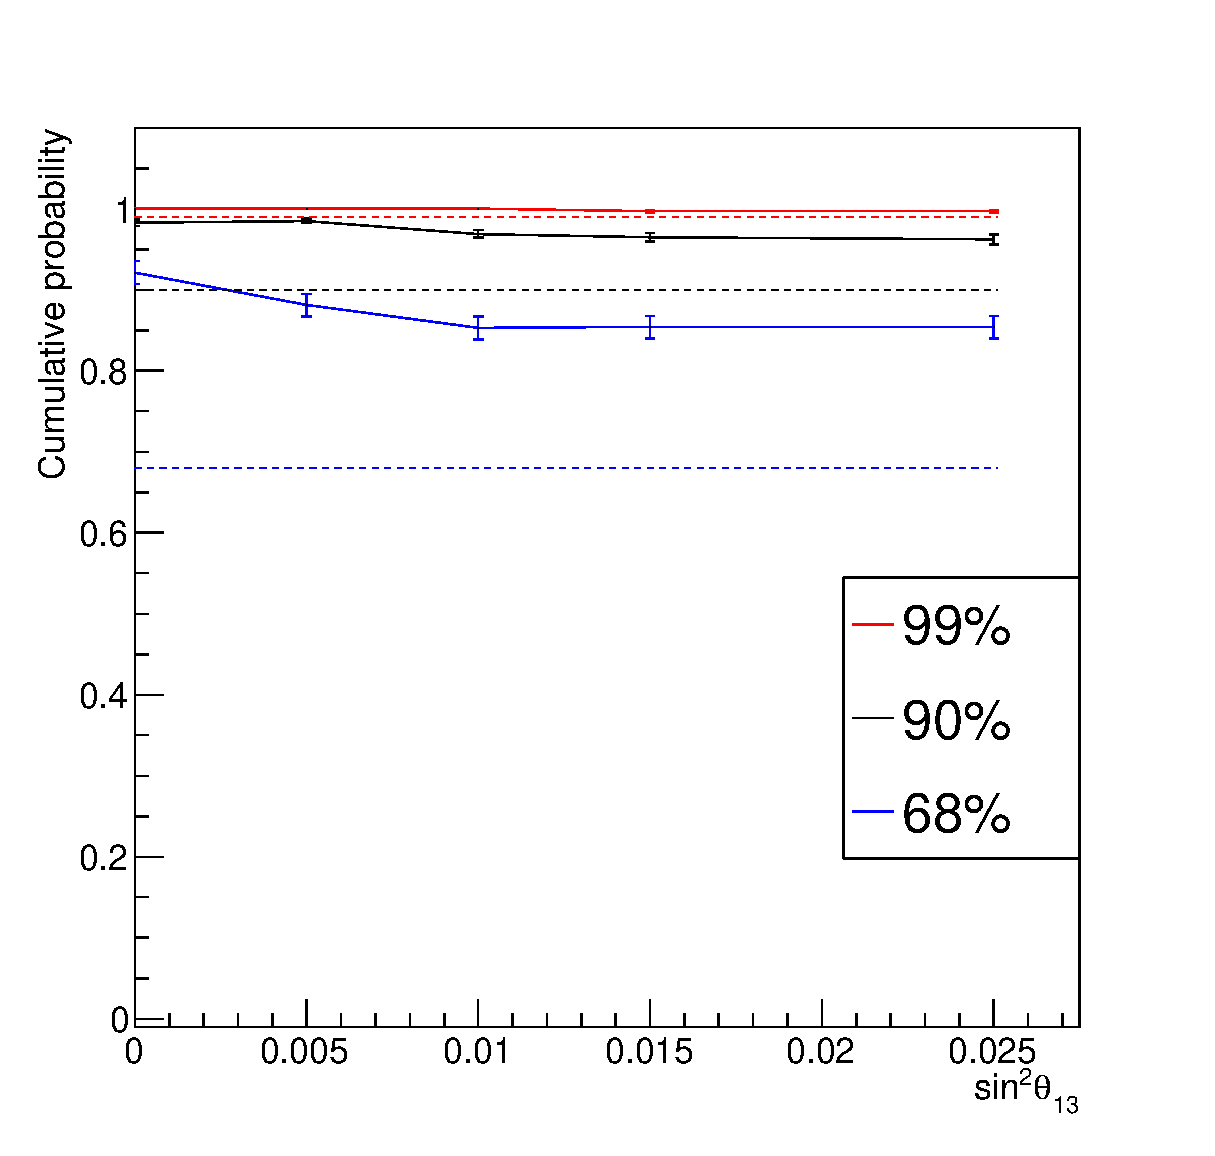
\includegraphics[width=14pc]{./images/appendix/coverage/coverage_study_2D_stats_theta13_deltacp_new_all.eps}
\center
\caption {
    Summary of figures \ref{fig:prob_2D_theta13_deltacp_0}-\ref{fig:prob_2D_theta13_deltacp_4}
showing the value of cumulative probability for $\Delta\chi^{2}=9.21$ (canonical value for 99\%), $\Delta\chi^{2}=4.61$ (canonical value for 90\%) and $\Delta\chi^{2}=2.30$ (canonical value for 68\%) vs the value of $sin^{2}\theta_{13}$.
	}
\label{fig:prob_2D_theta13_deltacp_all}
\end{minipage}
\end{figure*}
\end{center}



%% FIGURES FOR 2D theta13-theta23

\begin{center}
\begin{figure*}[htb]
\begin{minipage}[t]{0.46\linewidth}
\center
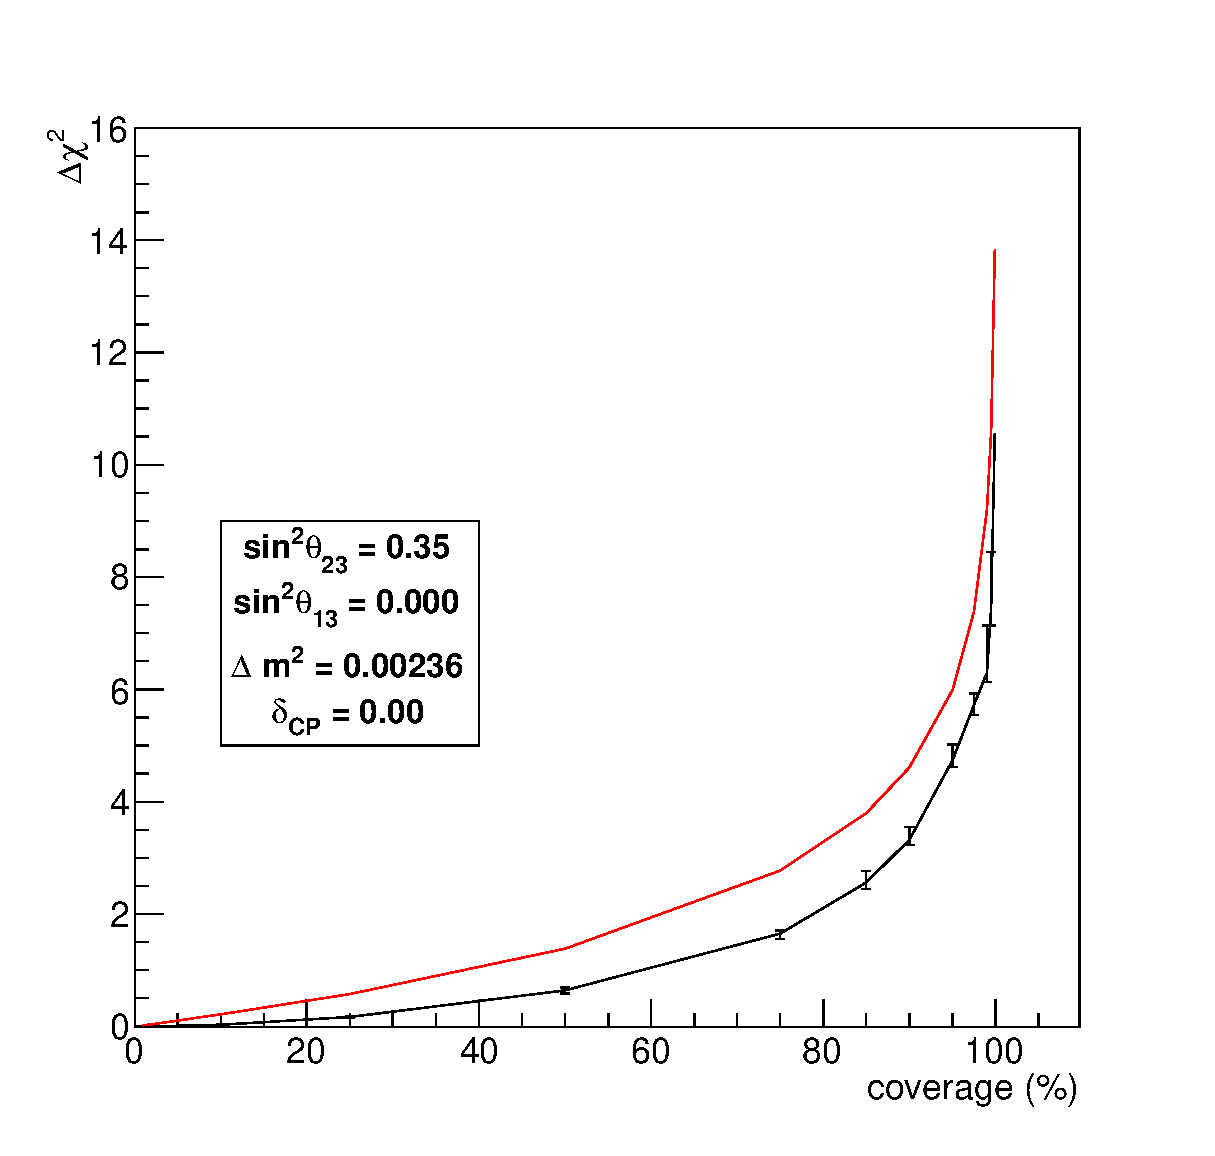
\includegraphics[width=14pc]{./images/appendix/coverage/coverage_study_2D_theta13_theta23_0.eps}
\center
\caption {
  Distribution of $\Delta\chi^{2}$ vs coverage in the ($sin^{2}\theta_{13}$,$sin^{2}\theta_{23}$) parameter space
  from 1k toy MC experiments generated with the Run 1+2+3 POT
  with statistical fluctuations at the oscillation point indicated in the legend. 
}
\label{fig:cov_2D_theta13_theta23_0}
\end{minipage}
\hspace{0.03\linewidth}
\begin{minipage}[t]{0.46\linewidth}
\center
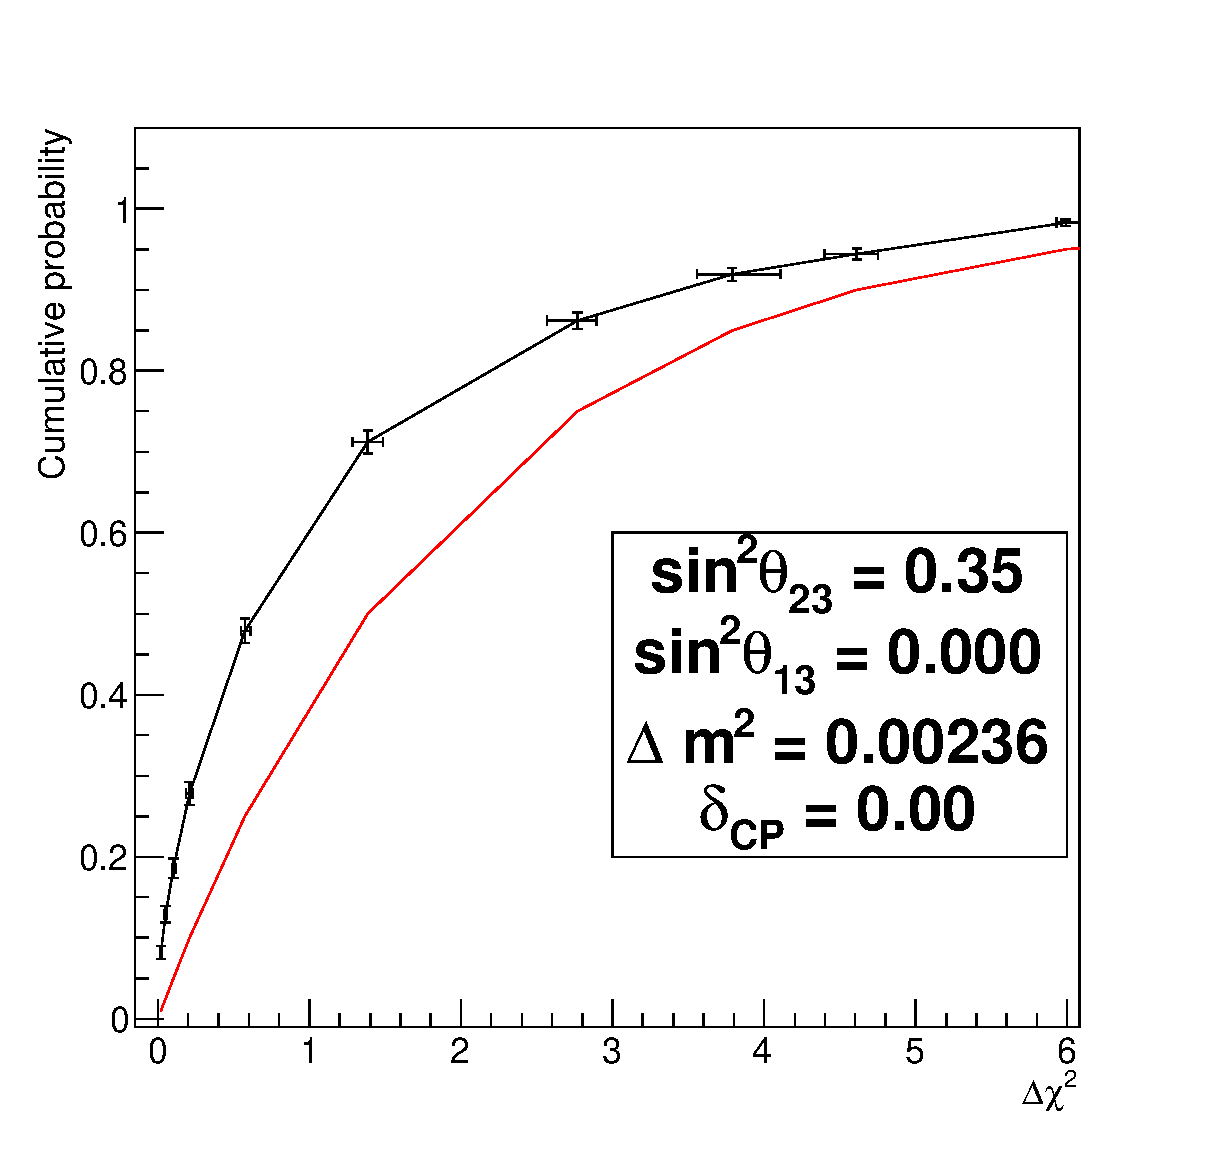
\includegraphics[width=14pc]{./images/appendix/coverage/coverage_study_2D_theta13_theta23_stats_new_0.eps}
\center
\caption {
  Distribution of cumulative probability vs $\Delta\chi^{2}$ in the ($sin^{2}\theta_{13}$,$sin^{2}\theta_{23}$) parameter space
  from 1k toy MC experiments generated with the Run 1+2+3 POT
  with statistical fluctuations at the oscillation point indicated in the legend. 
}
\label{fig:prob_2D_theta13_theta23_0}
\end{minipage}
\vfill
\vspace*{0.7cm}
\begin{minipage}[t]{0.46\linewidth}
\center
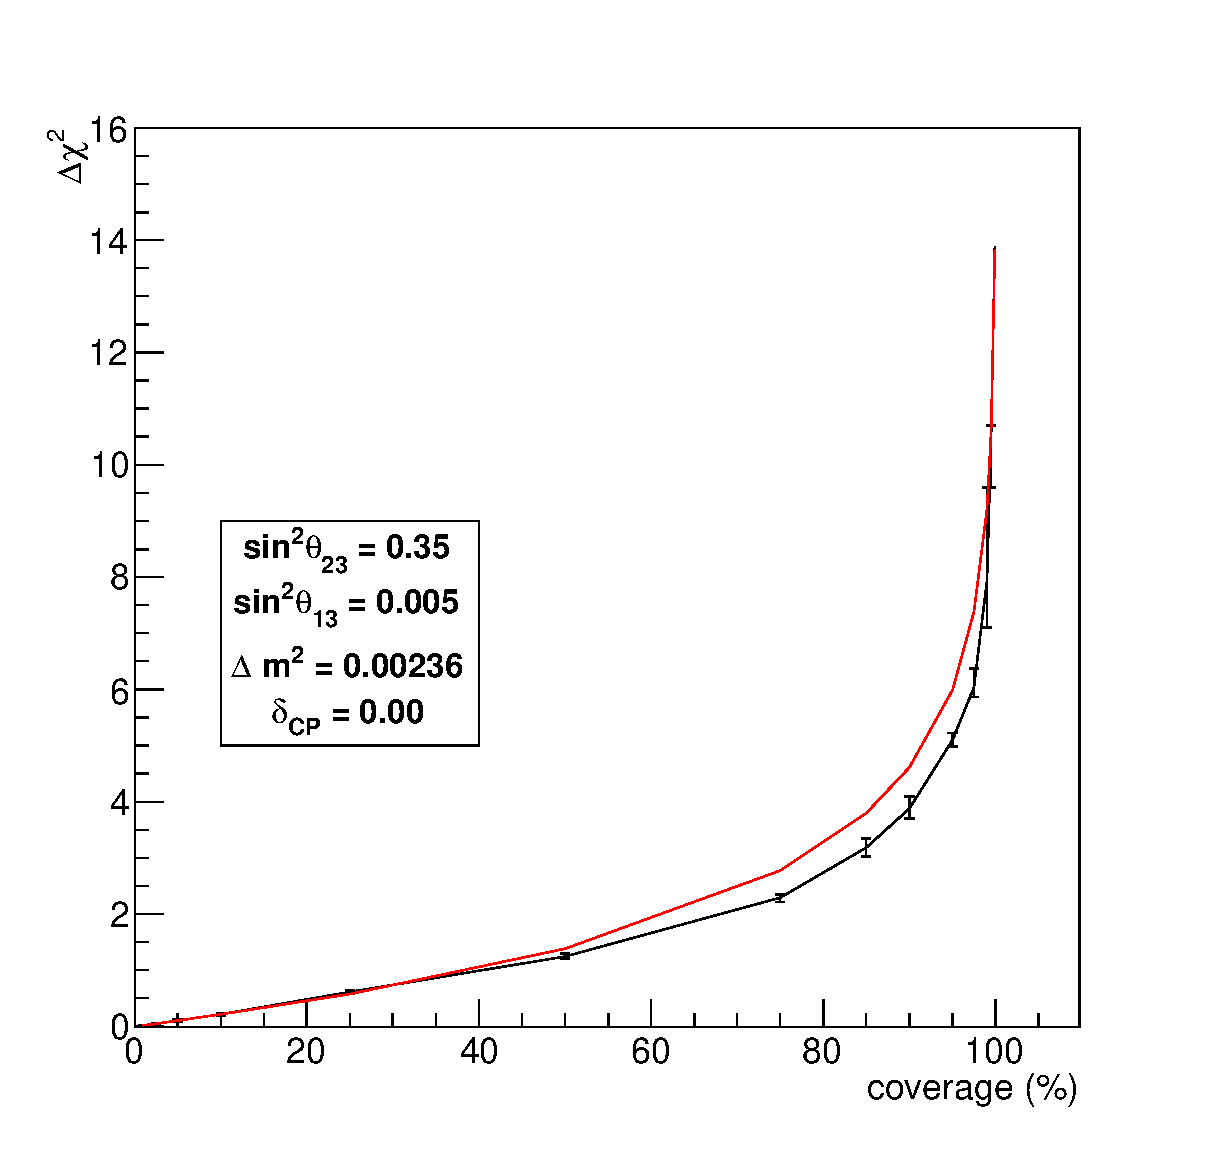
\includegraphics[width=14pc]{./images/appendix/coverage/coverage_study_2D_theta13_theta23_1.eps}
\center
\caption {
  Distribution of $\Delta\chi^{2}$ vs coverage in the ($sin^{2}\theta_{13}$,$sin^{2}\theta_{23}$) parameter space
  from 1k toy MC experiments generated with the Run 1+2+3 POT
  with statistical fluctuations at the oscillation point indicated in the legend. 
}
\label{fig:cov_2D_theta13_theta23_1}
\end{minipage}
\hspace{0.03\linewidth}
\begin{minipage}[t]{0.46\linewidth}
\center
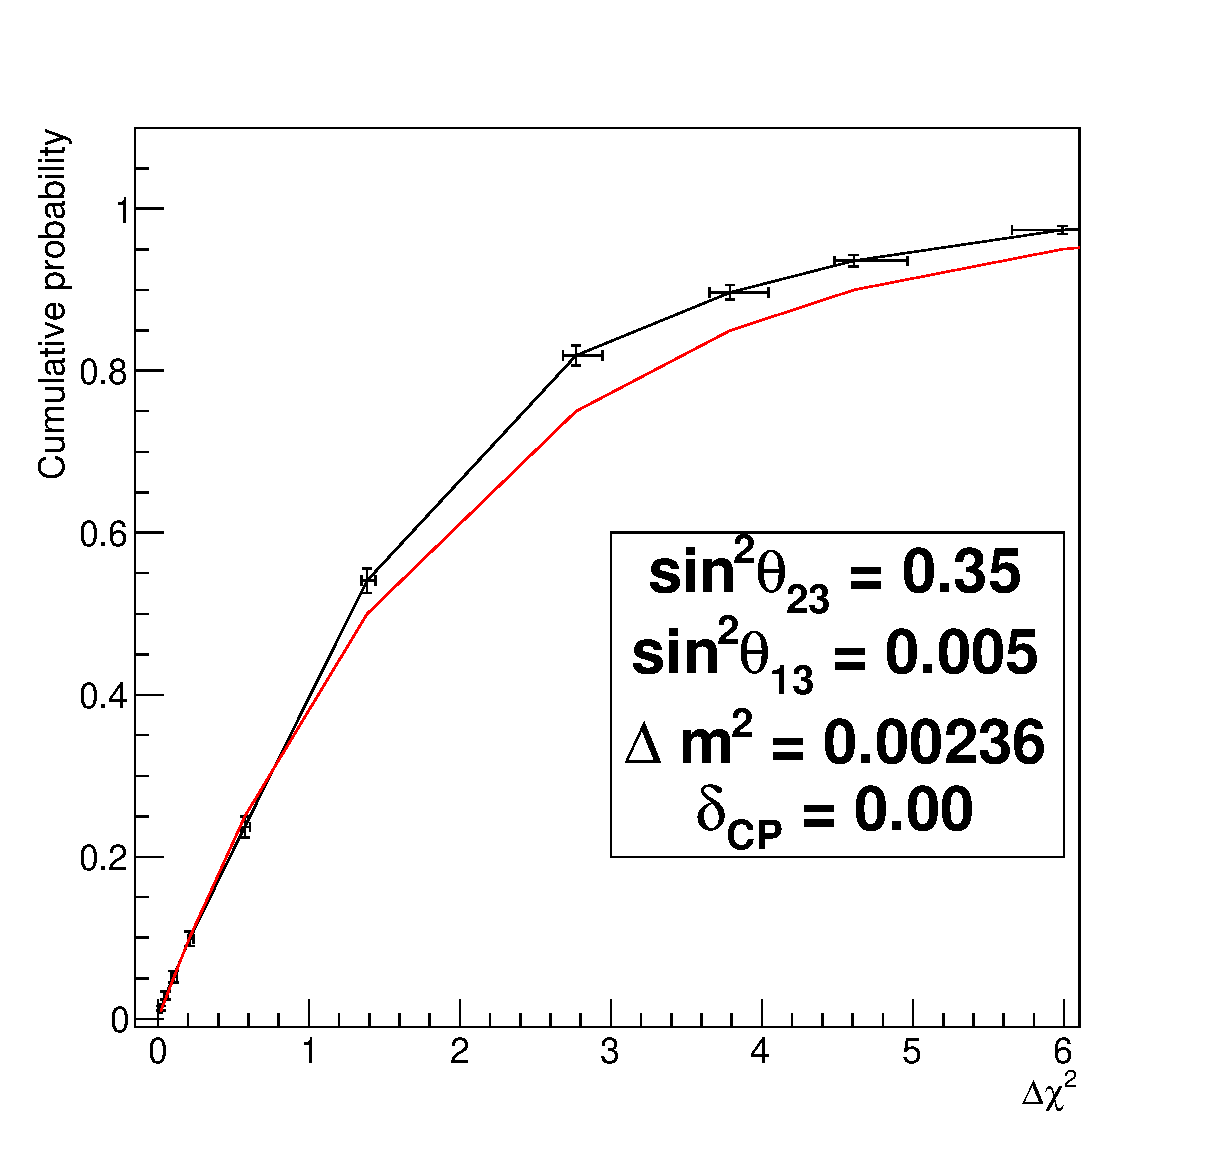
\includegraphics[width=14pc]{./images/appendix/coverage/coverage_study_2D_theta13_theta23_stats_new_1.eps}
\center
\caption {
  Distribution of cumulative probability vs $\Delta\chi^{2}$ in the ($sin^{2}\theta_{13}$,$sin^{2}\theta_{23}$) parameter space
  from 1k toy MC experiments generated with the Run 1+2+3 POT
  with statistical fluctuations at the oscillation point indicated in the legend. 
}
\label{fig:prob_2D_theta13_theta23_1}
\end{minipage}
\vfill
\vspace*{0.7cm}
\begin{minipage}[t]{0.46\linewidth}
\center
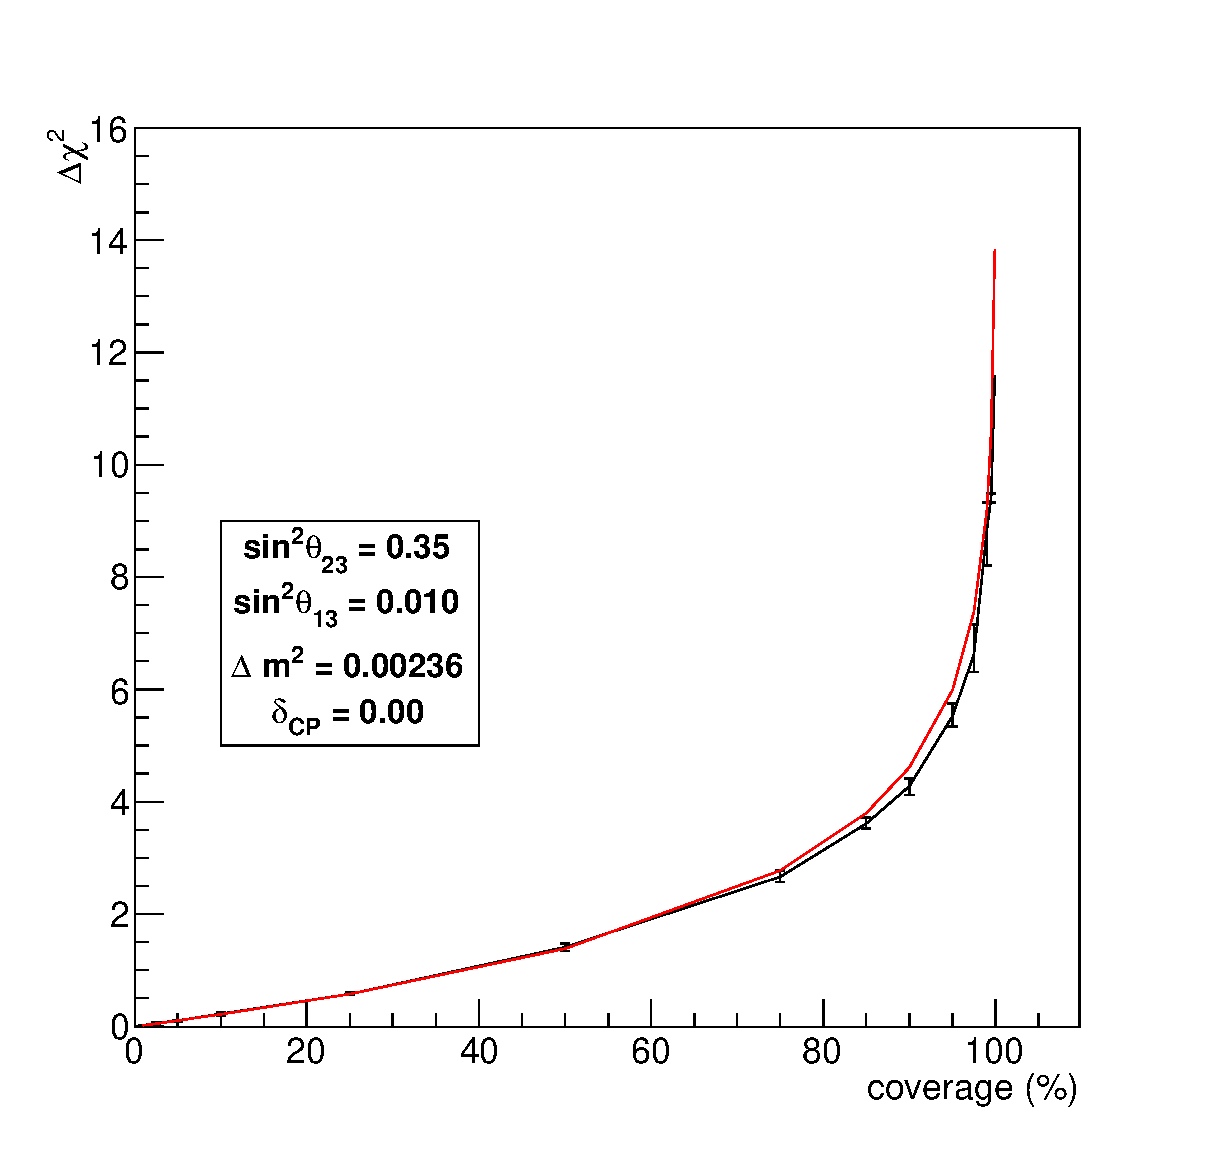
\includegraphics[width=14pc]{./images/appendix/coverage/coverage_study_2D_theta13_theta23_2.eps}
\center
\caption {
  Distribution of $\Delta\chi^{2}$ vs coverage in the ($sin^{2}\theta_{13}$,$sin^{2}\theta_{23}$) parameter space
  from 1k toy MC experiments generated with the Run 1+2+3 POT
  with statistical fluctuations at the oscillation point indicated in the legend. 
}
\label{fig:cov_2D_theta13_theta23_2}
\end{minipage}
\hspace{0.03\linewidth}
\begin{minipage}[t]{0.46\linewidth}
\center
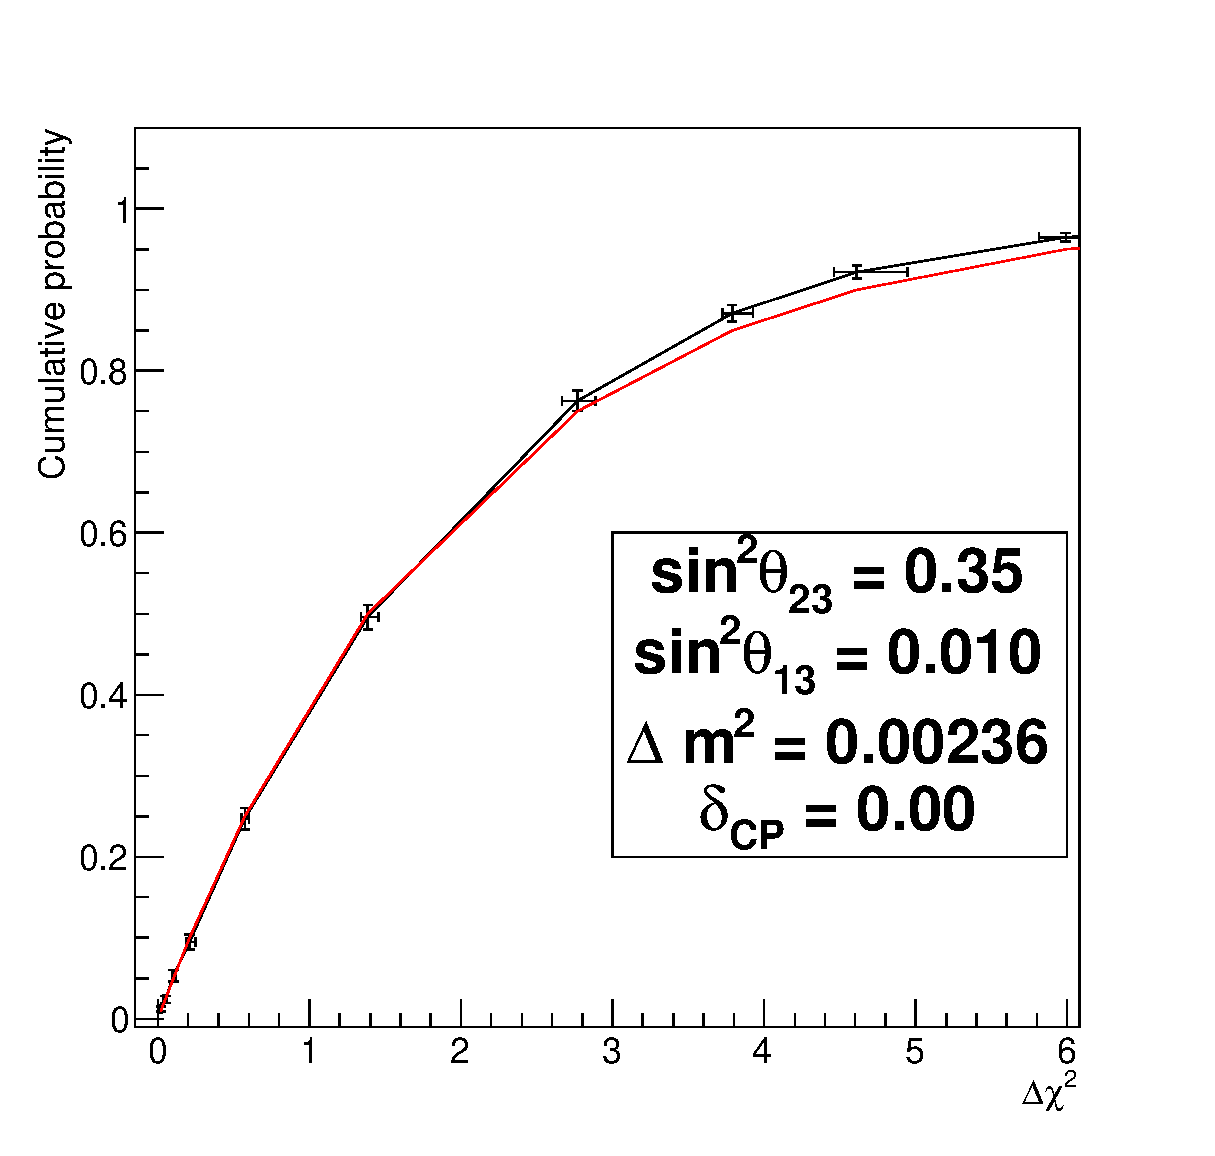
\includegraphics[width=14pc]{./images/appendix/coverage/coverage_study_2D_theta13_theta23_stats_new_2.eps}
\center
\caption {
  Distribution of cumulative probability vs $\Delta\chi^{2}$ in the ($sin^{2}\theta_{13}$,$sin^{2}\theta_{23}$) parameter space
  from 1k toy MC experiments generated with the Run 1+2+3 POT
  with statistical fluctuations at the oscillation point indicated in the legend. 
}
\label{fig:prob_2D_theta13_theta23_2}
\end{minipage}
\end{figure*}
\end{center}



\begin{center}
\begin{figure*}[htb]
\begin{minipage}[t]{0.46\linewidth}
\center
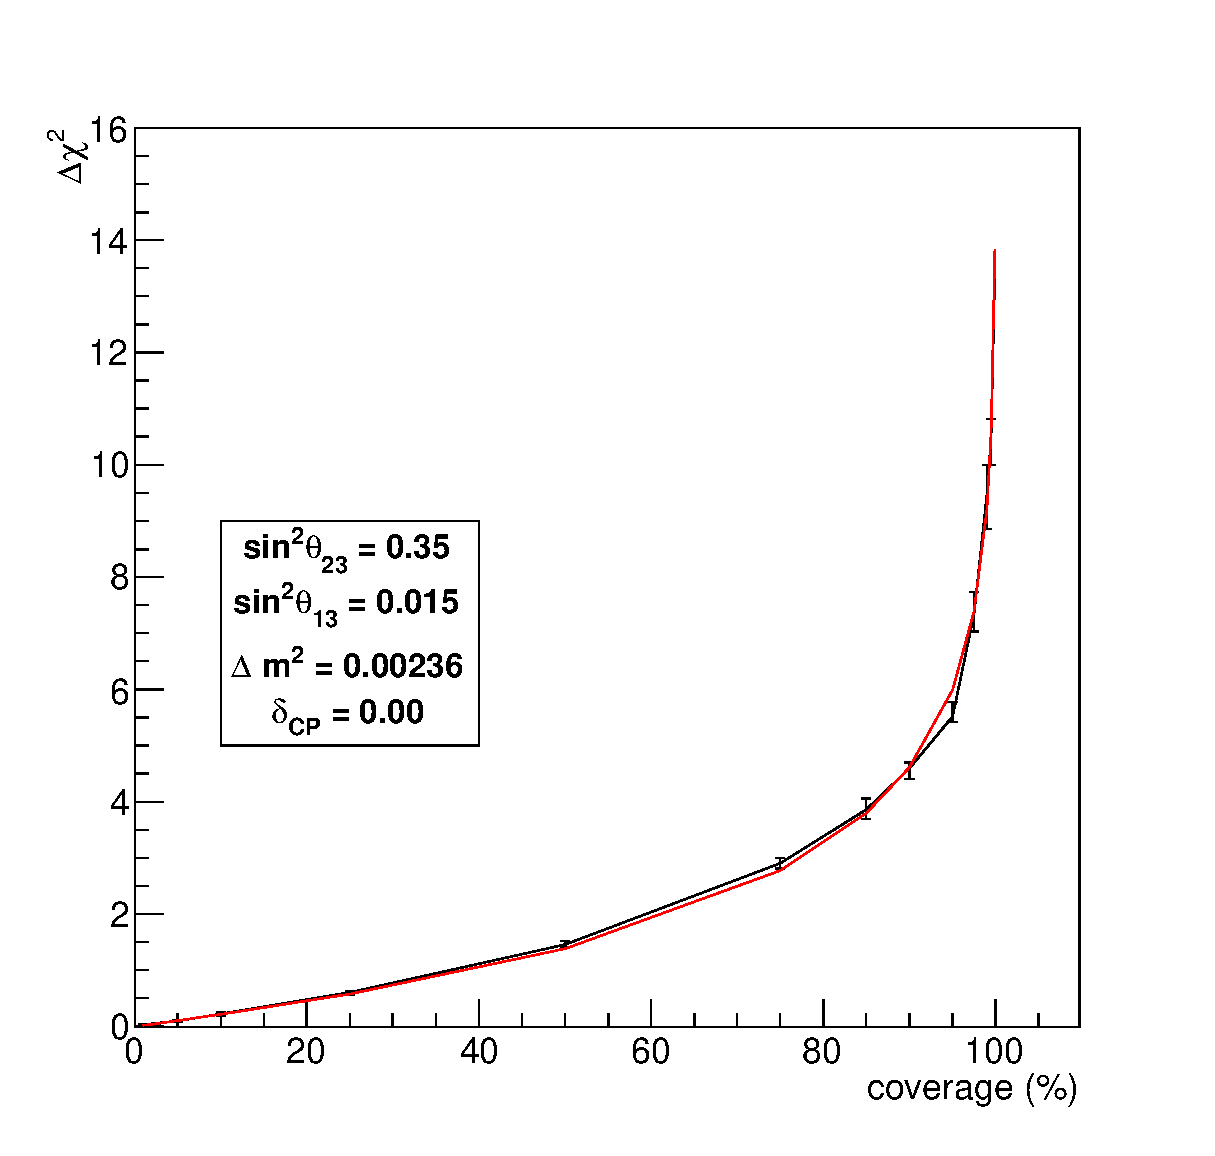
\includegraphics[width=14pc]{./images/appendix/coverage/coverage_study_2D_theta13_theta23_3.eps}
\center
\caption {
  Distribution of $\Delta\chi^{2}$ vs coverage in the ($sin^{2}\theta_{13}$,$sin^{2}\theta_{23}$) parameter space
  from 1k toy MC experiments generated with the Run 1+2+3 POT
  with statistical fluctuations at the oscillation point indicated in the legend. 
}
\label{fig:cov_2D_theta13_theta23_3}
\end{minipage}
\hspace{0.03\linewidth}
\begin{minipage}[t]{0.46\linewidth}
\center
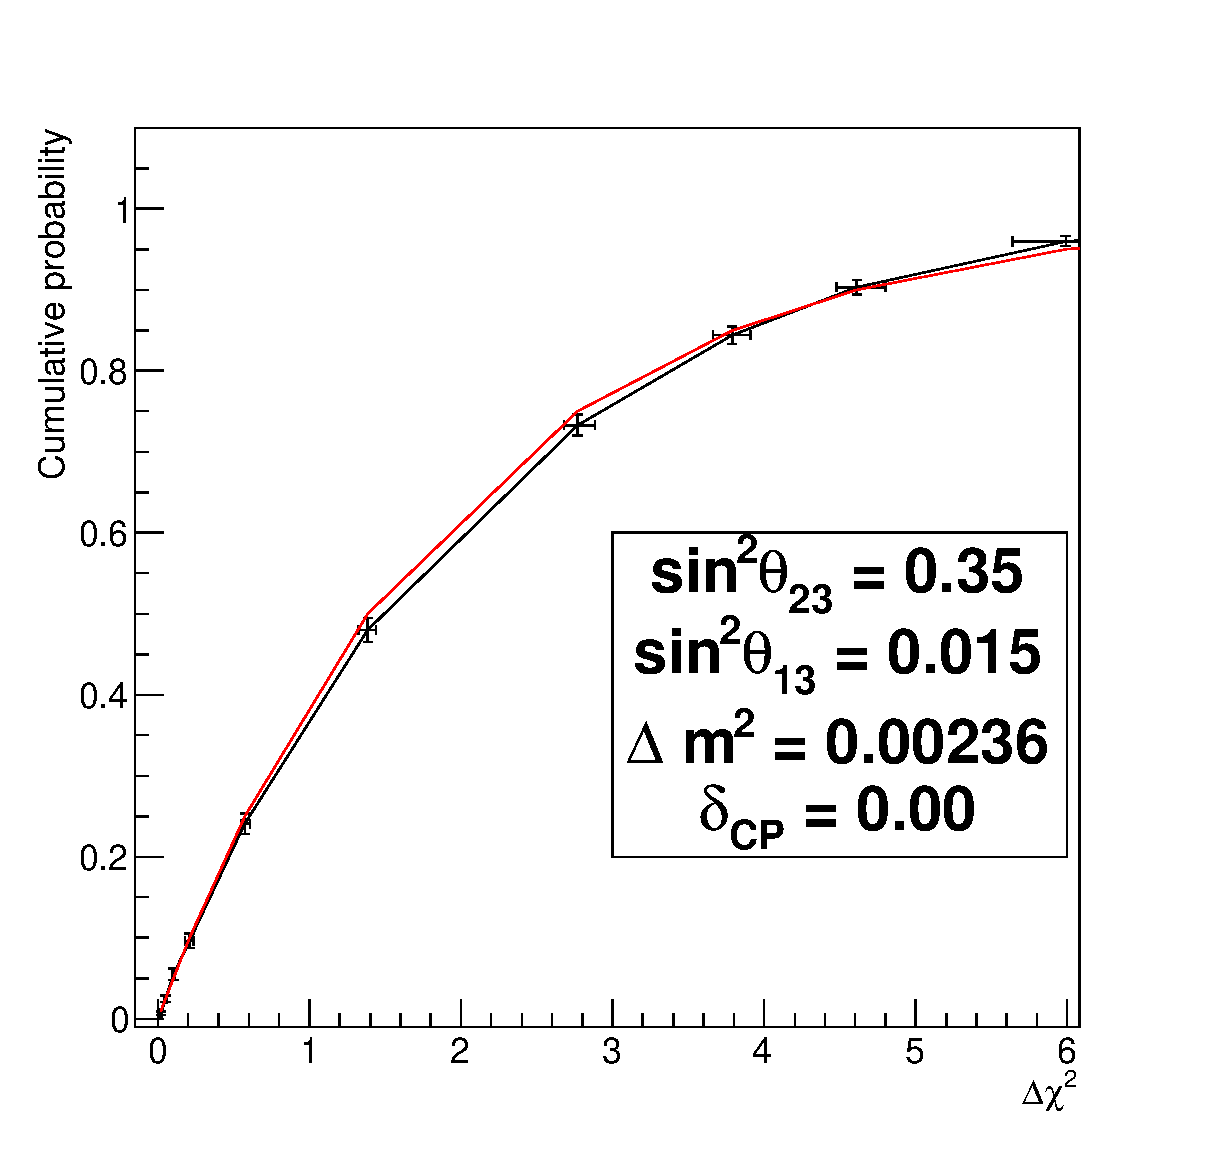
\includegraphics[width=14pc]{./images/appendix/coverage/coverage_study_2D_theta13_theta23_stats_new_3.eps}
\center
\caption {
  Distribution of cumulative probability vs $\Delta\chi^{2}$ in the ($sin^{2}\theta_{13}$,$sin^{2}\theta_{23}$) parameter space
  from 1k toy MC experiments generated with the Run 1+2+3 POT
  with statistical fluctuations at the oscillation point indicated in the legend. 
}
\label{fig:prob_2D_theta13_theta23_3}
\end{minipage}
\vfill
\vspace*{0.7cm}
\begin{minipage}[t]{0.46\linewidth}
\center
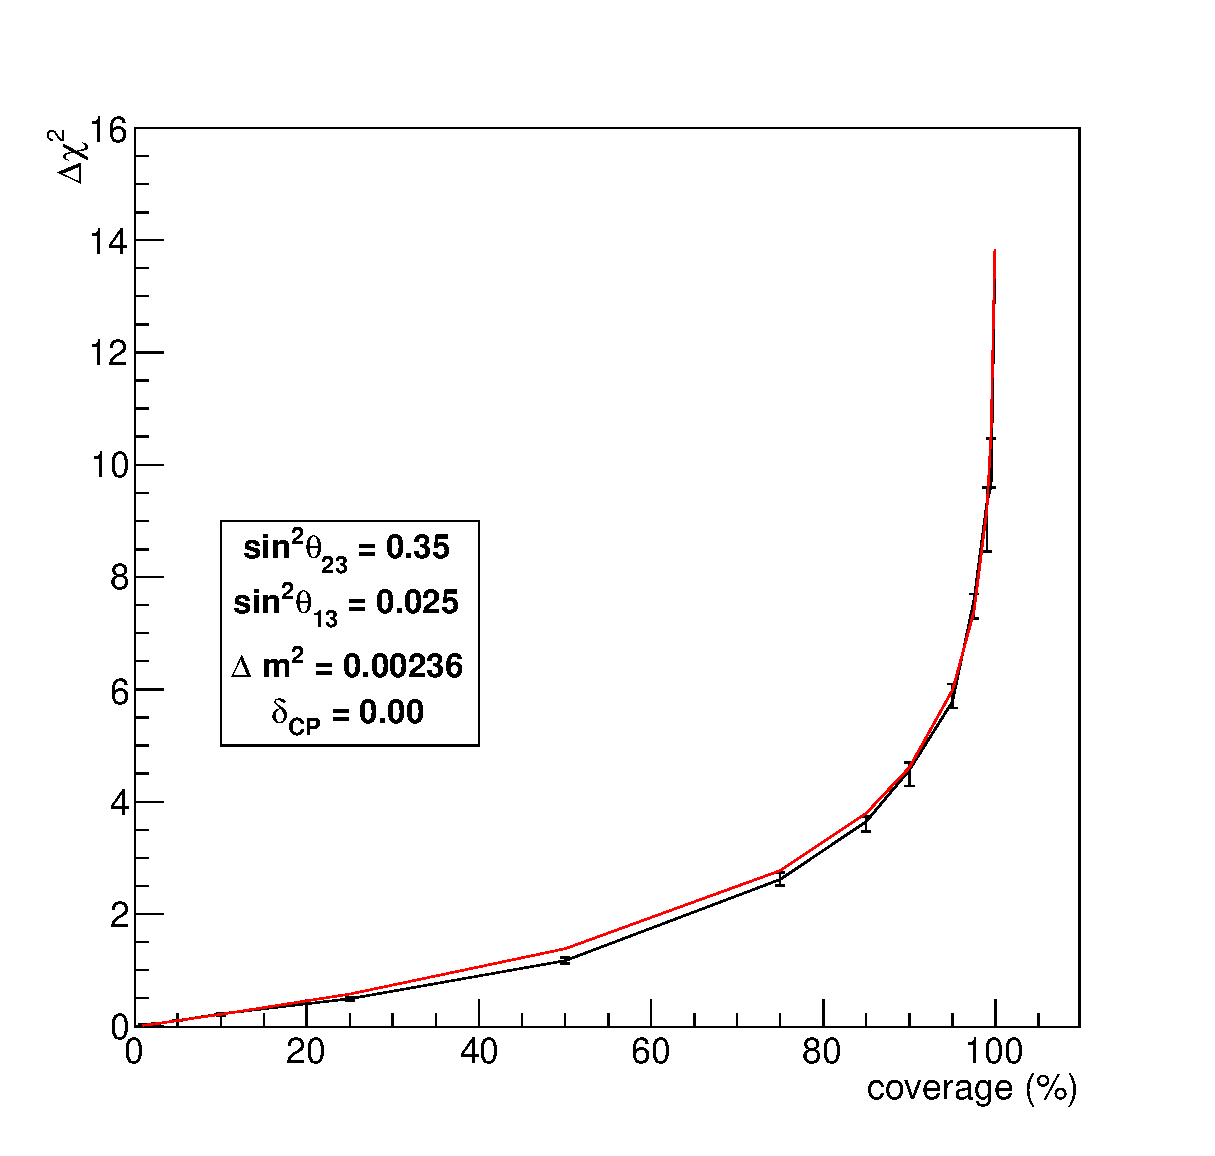
\includegraphics[width=14pc]{./images/appendix/coverage/coverage_study_2D_theta13_theta23_4.eps}
\center
\caption {
  Distribution of $\Delta\chi^{2}$ vs coverage in the ($sin^{2}\theta_{13}$,$sin^{2}\theta_{23}$) parameter space
  from 1k toy MC experiments generated with the Run 1+2+3 POT
  with statistical fluctuations at the oscillation point indicated in the legend. 
}
\label{fig:cov_2D_theta13_theta23_4}
\end{minipage}
\hspace{0.03\linewidth}
\begin{minipage}[t]{0.46\linewidth}
\center
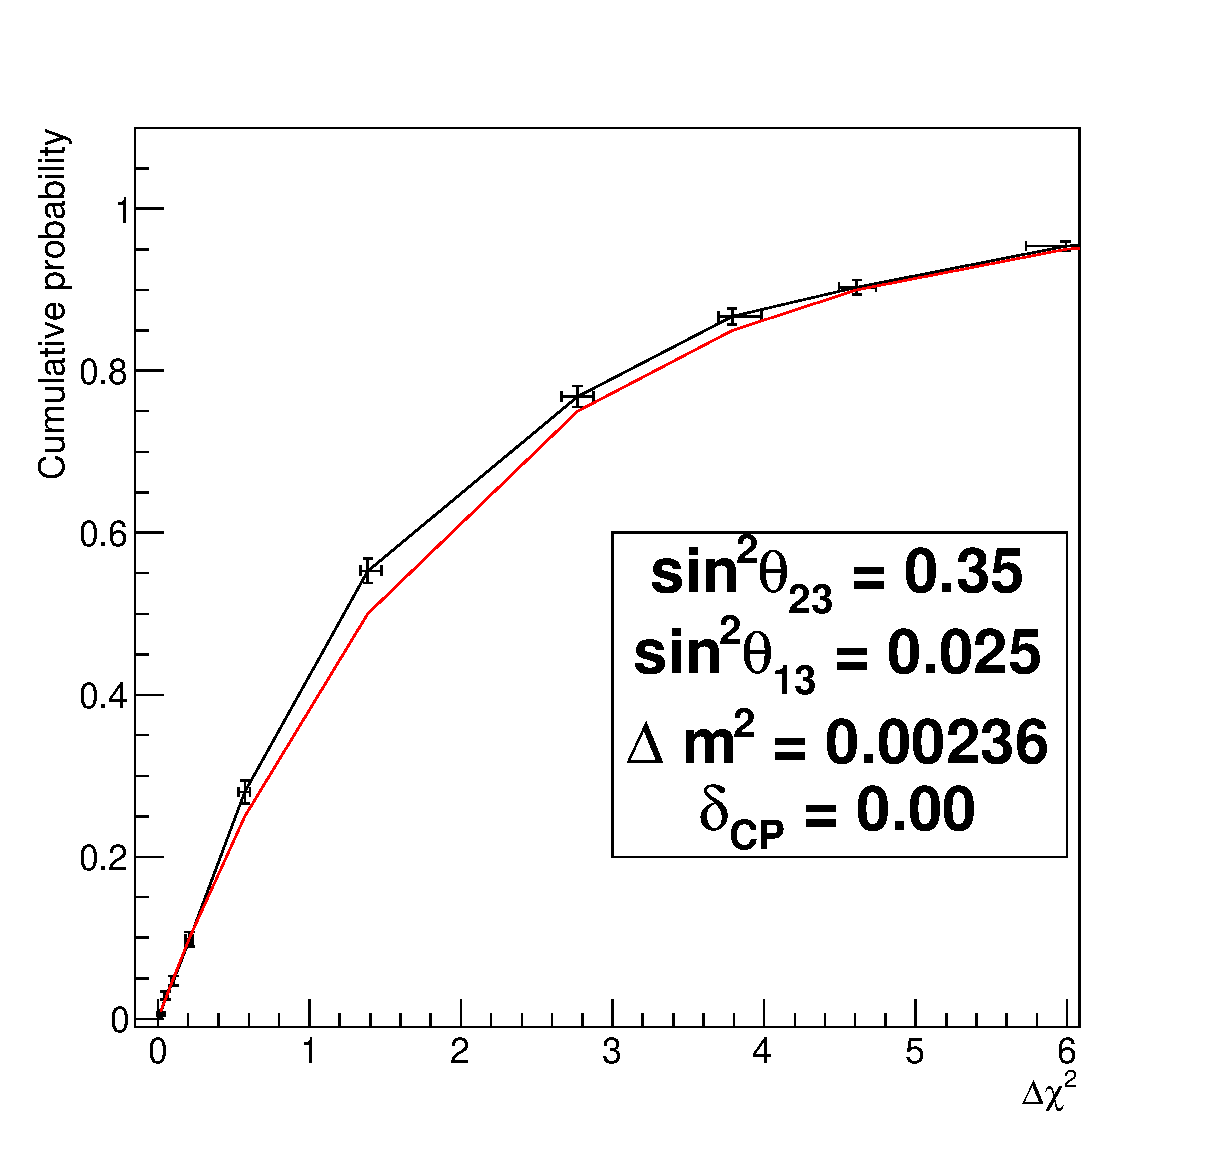
\includegraphics[width=14pc]{./images/appendix/coverage/coverage_study_2D_theta13_theta23_stats_new_4.eps}
\center
\caption {
  Distribution of cumulative probability vs $\Delta\chi^{2}$ in the ($sin^{2}\theta_{13}$,$sin^{2}\theta_{23}$) parameter space
  from 1k toy MC experiments generated with the Run 1+2+3 POT
  with statistical fluctuations at the oscillation point indicated in the legend. 
}
\label{fig:prob_2D_theta13_theta23_4}
\end{minipage}
\vfill
\vspace*{0.7cm}
\begin{minipage}[t]{0.46\linewidth}
\center
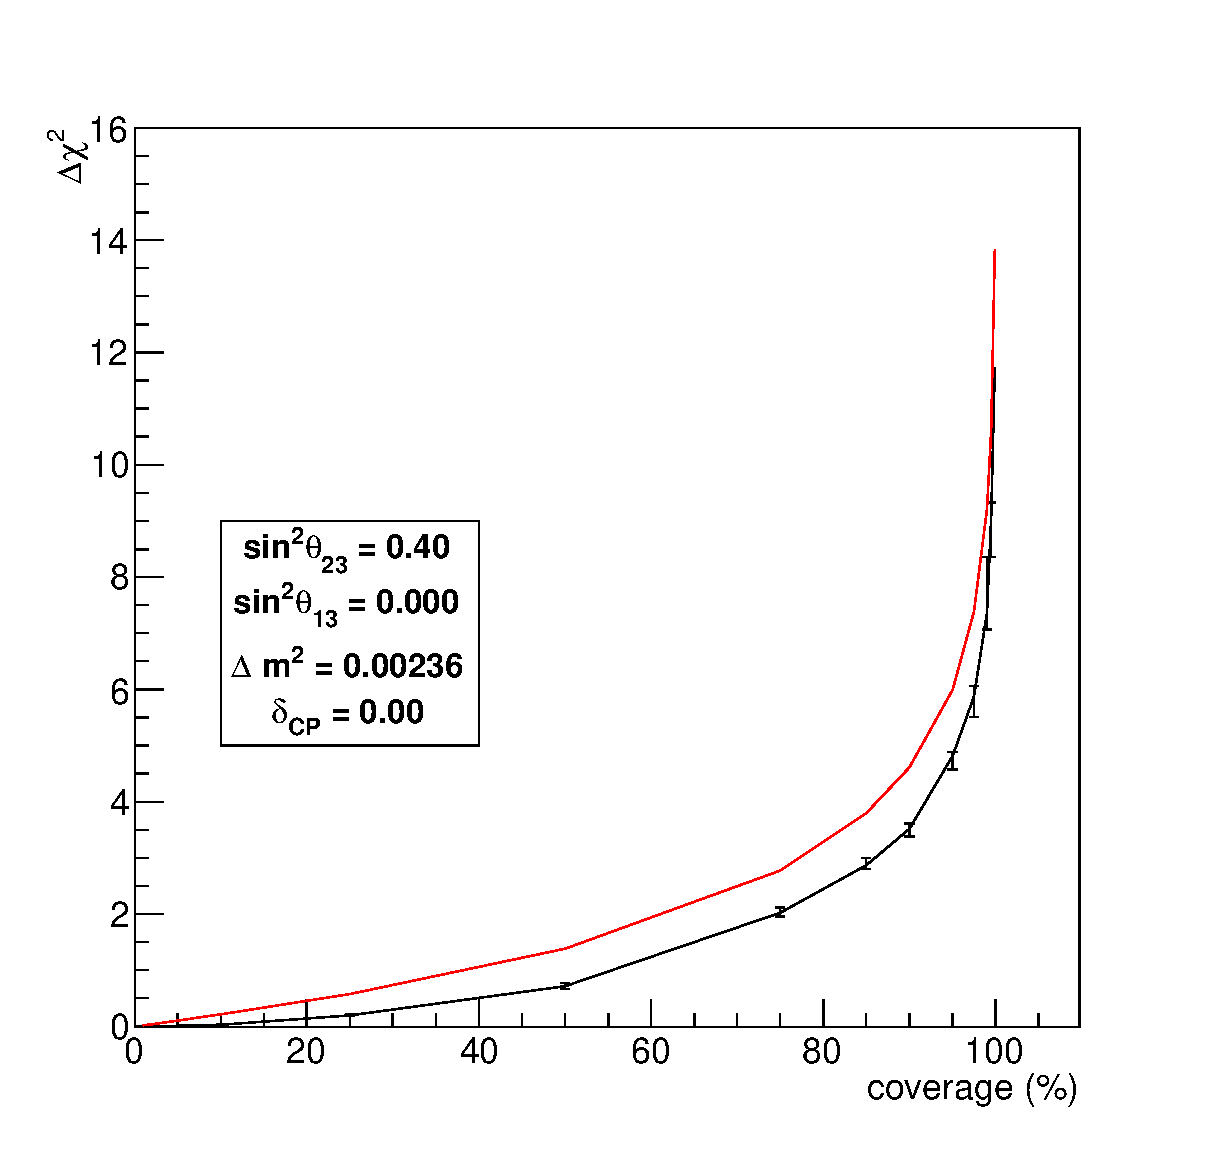
\includegraphics[width=14pc]{./images/appendix/coverage/coverage_study_2D_theta13_theta23_5.eps}
\center
\caption {
  Distribution of $\Delta\chi^{2}$ vs coverage in the ($sin^{2}\theta_{13}$,$sin^{2}\theta_{23}$) parameter space
  from 1k toy MC experiments generated with the Run 1+2+3 POT
  with statistical fluctuations at the oscillation point indicated in the legend. 
}
\label{fig:cov_2D_theta13_theta23_5}
\end{minipage}
\hspace{0.03\linewidth}
\begin{minipage}[t]{0.46\linewidth}
\center
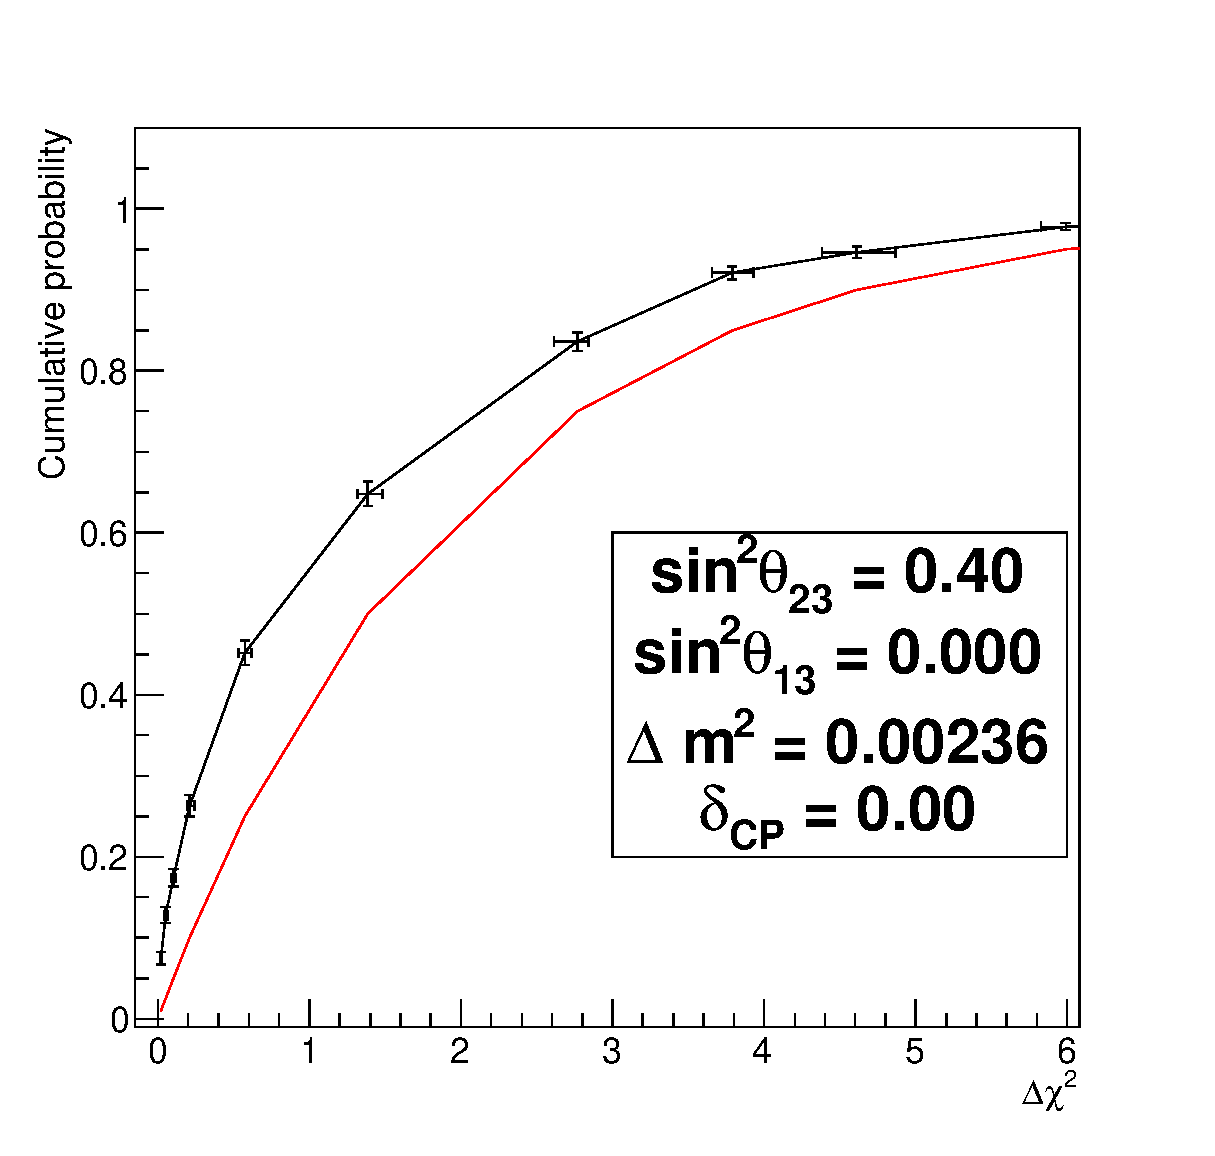
\includegraphics[width=14pc]{./images/appendix/coverage/coverage_study_2D_theta13_theta23_stats_new_5.eps}
\center
\caption {
  Distribution of cumulative probability vs $\Delta\chi^{2}$ in the ($sin^{2}\theta_{13}$,$sin^{2}\theta_{23}$) parameter space
  from 1k toy MC experiments generated with the Run 1+2+3 POT
  with statistical fluctuations at the oscillation point indicated in the legend. 
}
\label{fig:prob_2D_theta13_theta23_5}
\end{minipage}
\end{figure*}
\end{center}


\begin{center}
\begin{figure*}[htb]
\begin{minipage}[t]{0.46\linewidth}
\center
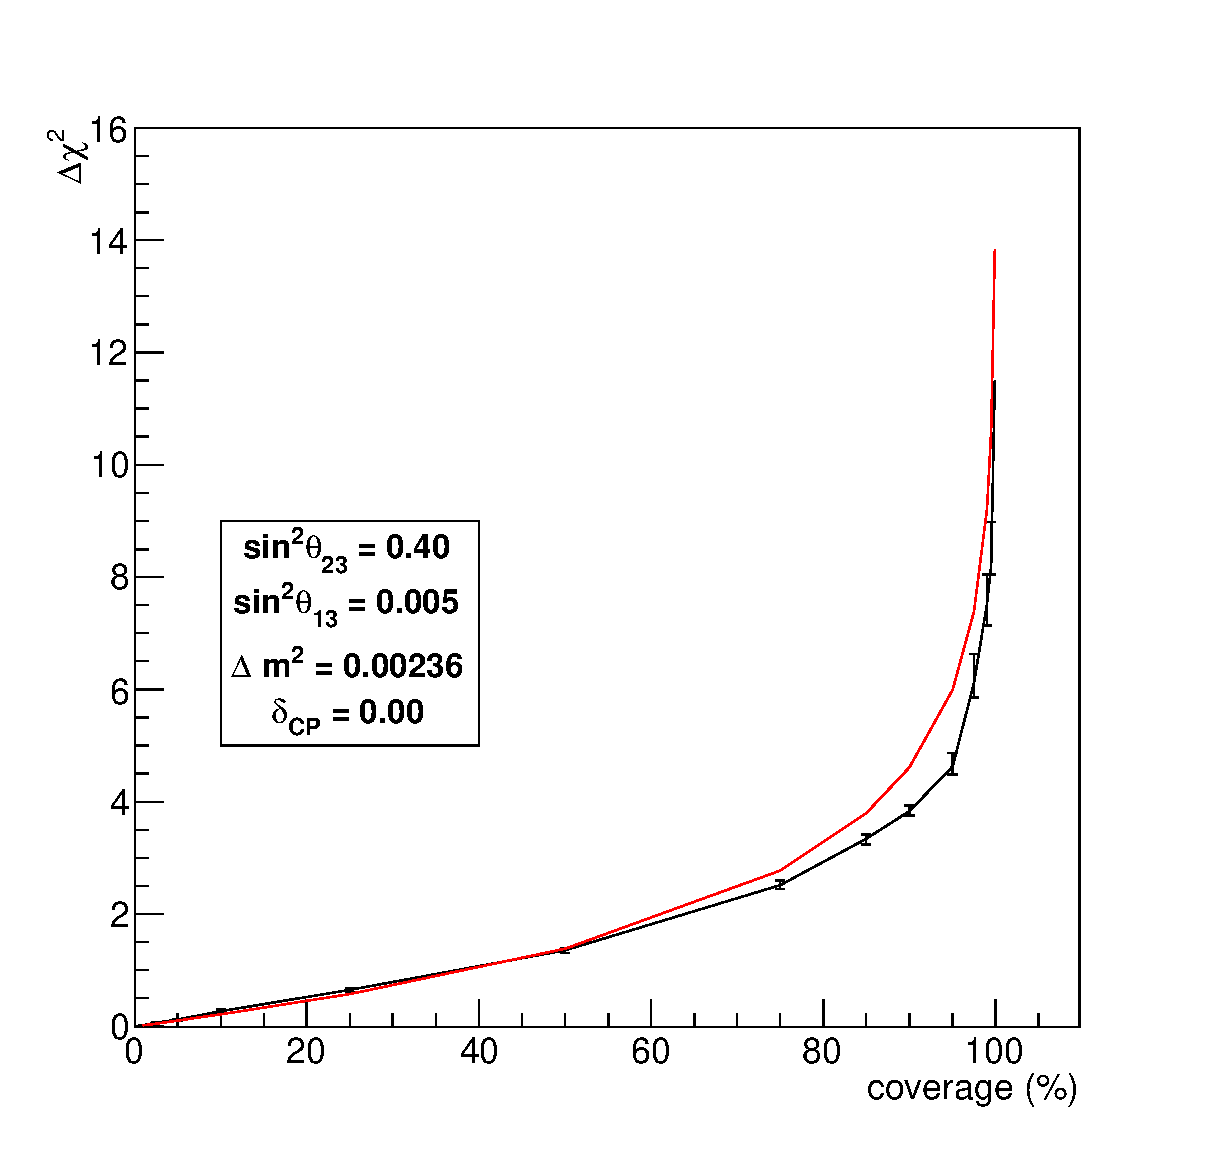
\includegraphics[width=14pc]{./images/appendix/coverage/coverage_study_2D_theta13_theta23_6.eps}
\center
\caption {
  Distribution of $\Delta\chi^{2}$ vs coverage in the ($sin^{2}\theta_{13}$,$sin^{2}\theta_{23}$) parameter space
  from 1k toy MC experiments generated with the Run 1+2+3 POT
  with statistical fluctuations at the oscillation point indicated in the legend. 
}
\label{fig:cov_2D_theta13_theta23_6}
\end{minipage}
\hspace{0.03\linewidth}
\begin{minipage}[t]{0.46\linewidth}
\center
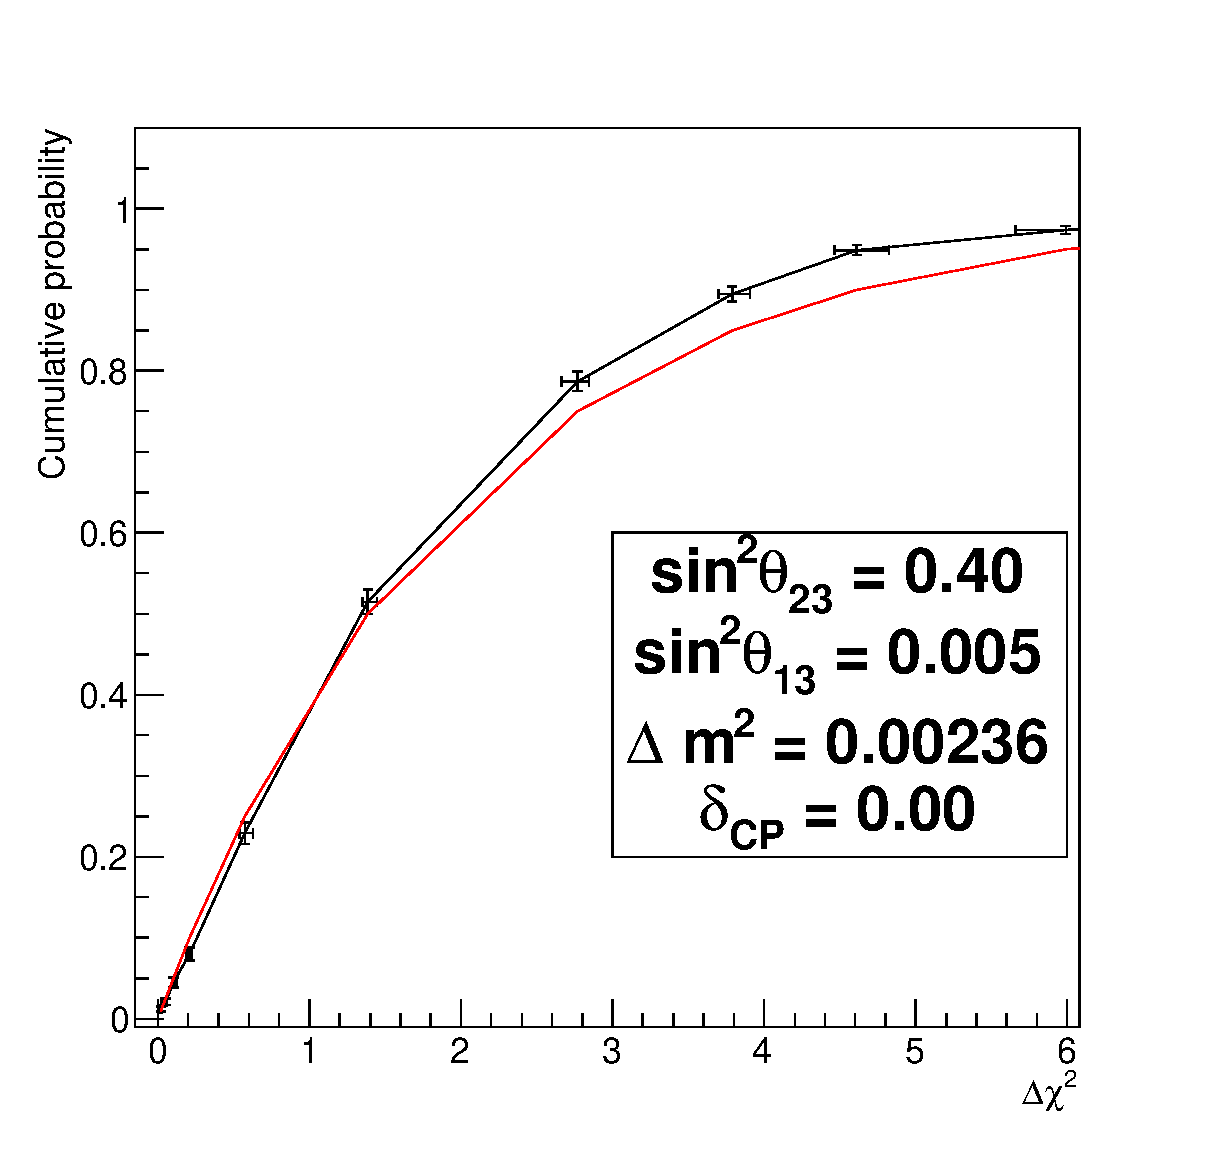
\includegraphics[width=14pc]{./images/appendix/coverage/coverage_study_2D_theta13_theta23_stats_new_6.eps}
\center
\caption {
  Distribution of cumulative probability vs $\Delta\chi^{2}$ in the ($sin^{2}\theta_{13}$,$sin^{2}\theta_{23}$) parameter space
  from 1k toy MC experiments generated with the Run 1+2+3 POT
  with statistical fluctuations at the oscillation point indicated in the legend. 
}
\label{fig:prob_2D_theta13_theta23_6}
\end{minipage}
\vfill
\vspace*{0.7cm}
\begin{minipage}[t]{0.46\linewidth}
\center
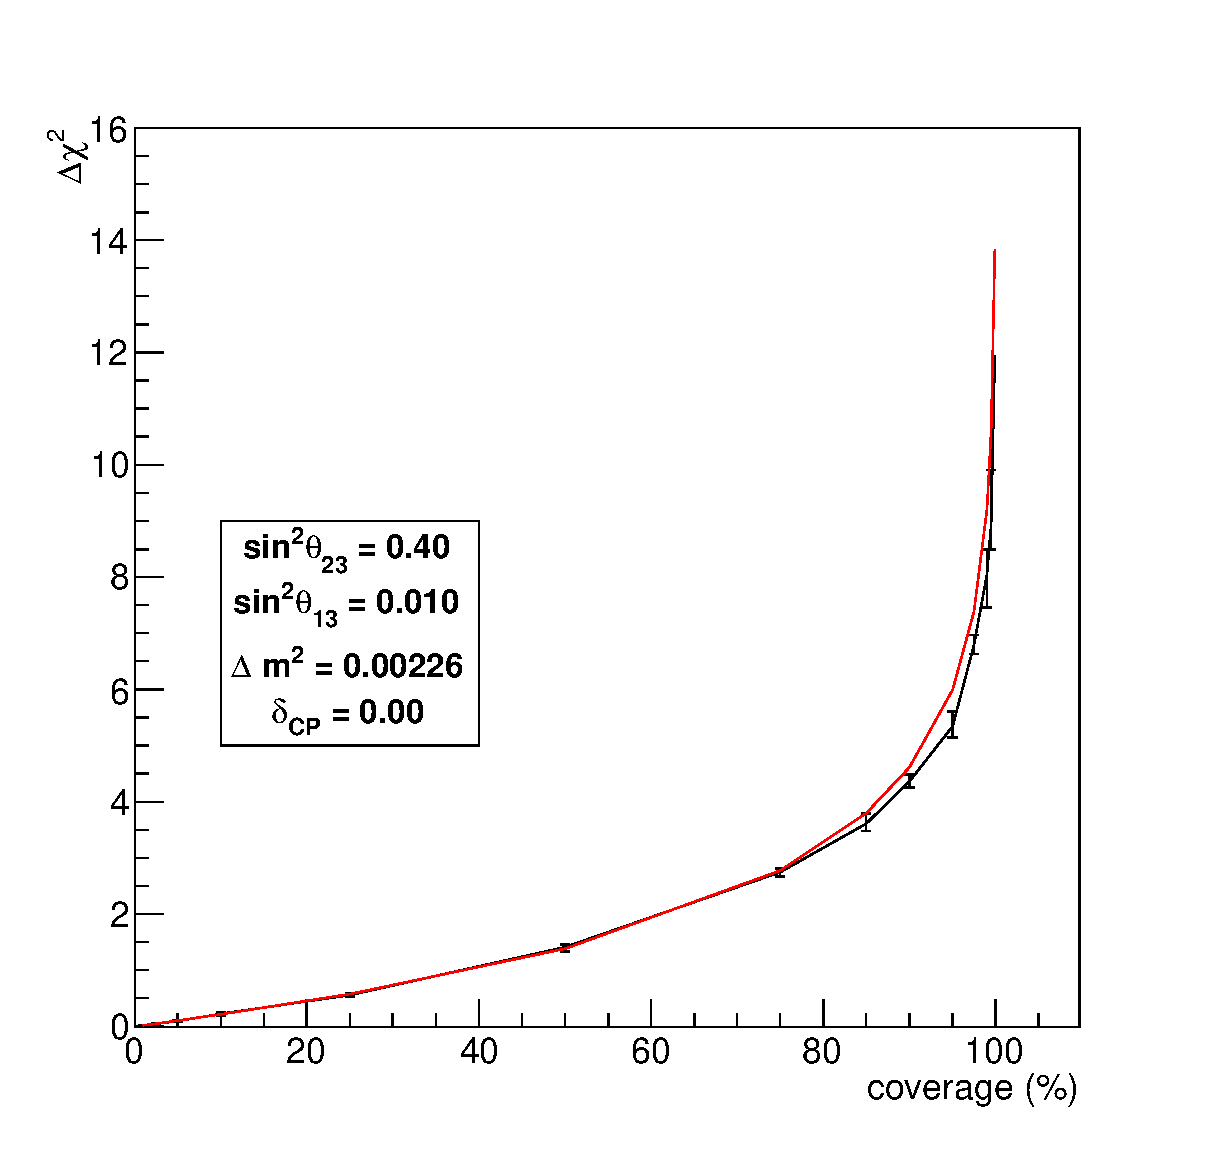
\includegraphics[width=14pc]{./images/appendix/coverage/coverage_study_2D_theta13_theta23_7.eps}
\center
\caption {
  Distribution of $\Delta\chi^{2}$ vs coverage in the ($sin^{2}\theta_{13}$,$sin^{2}\theta_{23}$) parameter space
  from 1k toy MC experiments generated with the Run 1+2+3 POT
  with statistical fluctuations at the oscillation point indicated in the legend. 
}
\label{fig:cov_2D_theta13_theta23_7}
\end{minipage}
\hspace{0.03\linewidth}
\begin{minipage}[t]{0.46\linewidth}
\center
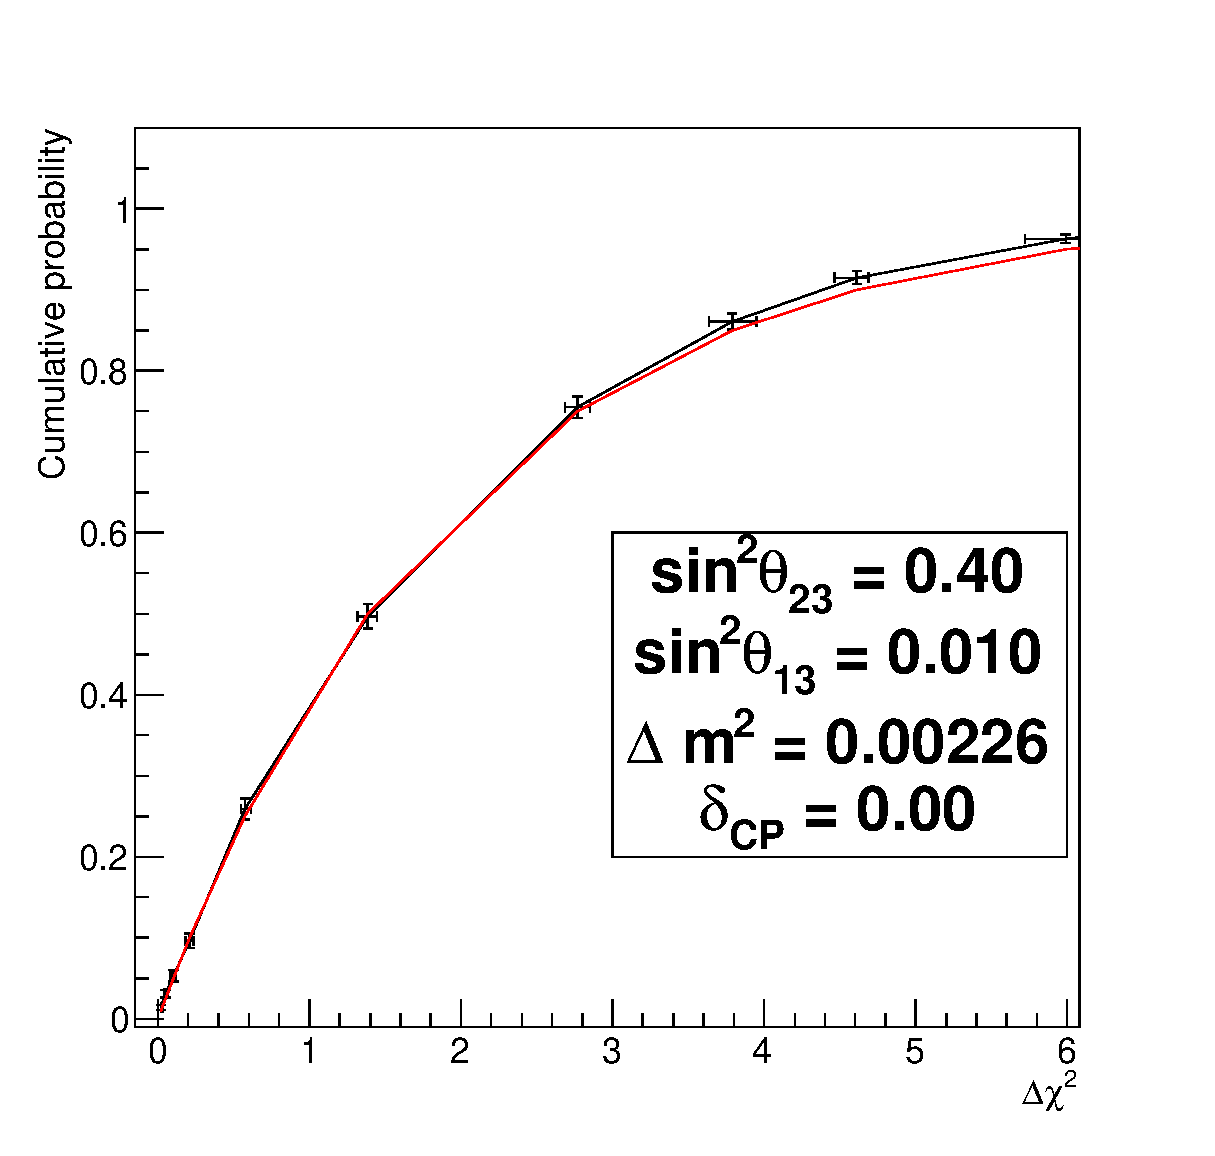
\includegraphics[width=14pc]{./images/appendix/coverage/coverage_study_2D_theta13_theta23_stats_new_7.eps}
\center
\caption {
  Distribution of cumulative probability vs $\Delta\chi^{2}$ in the ($sin^{2}\theta_{13}$,$sin^{2}\theta_{23}$) parameter space
  from 1k toy MC experiments generated with the Run 1+2+3 POT
  with statistical fluctuations at the oscillation point indicated in the legend. 
}
\label{fig:prob_2D_theta13_theta23_7}
\end{minipage}
\vfill
\vspace*{0.7cm}
\begin{minipage}[t]{0.46\linewidth}
\center
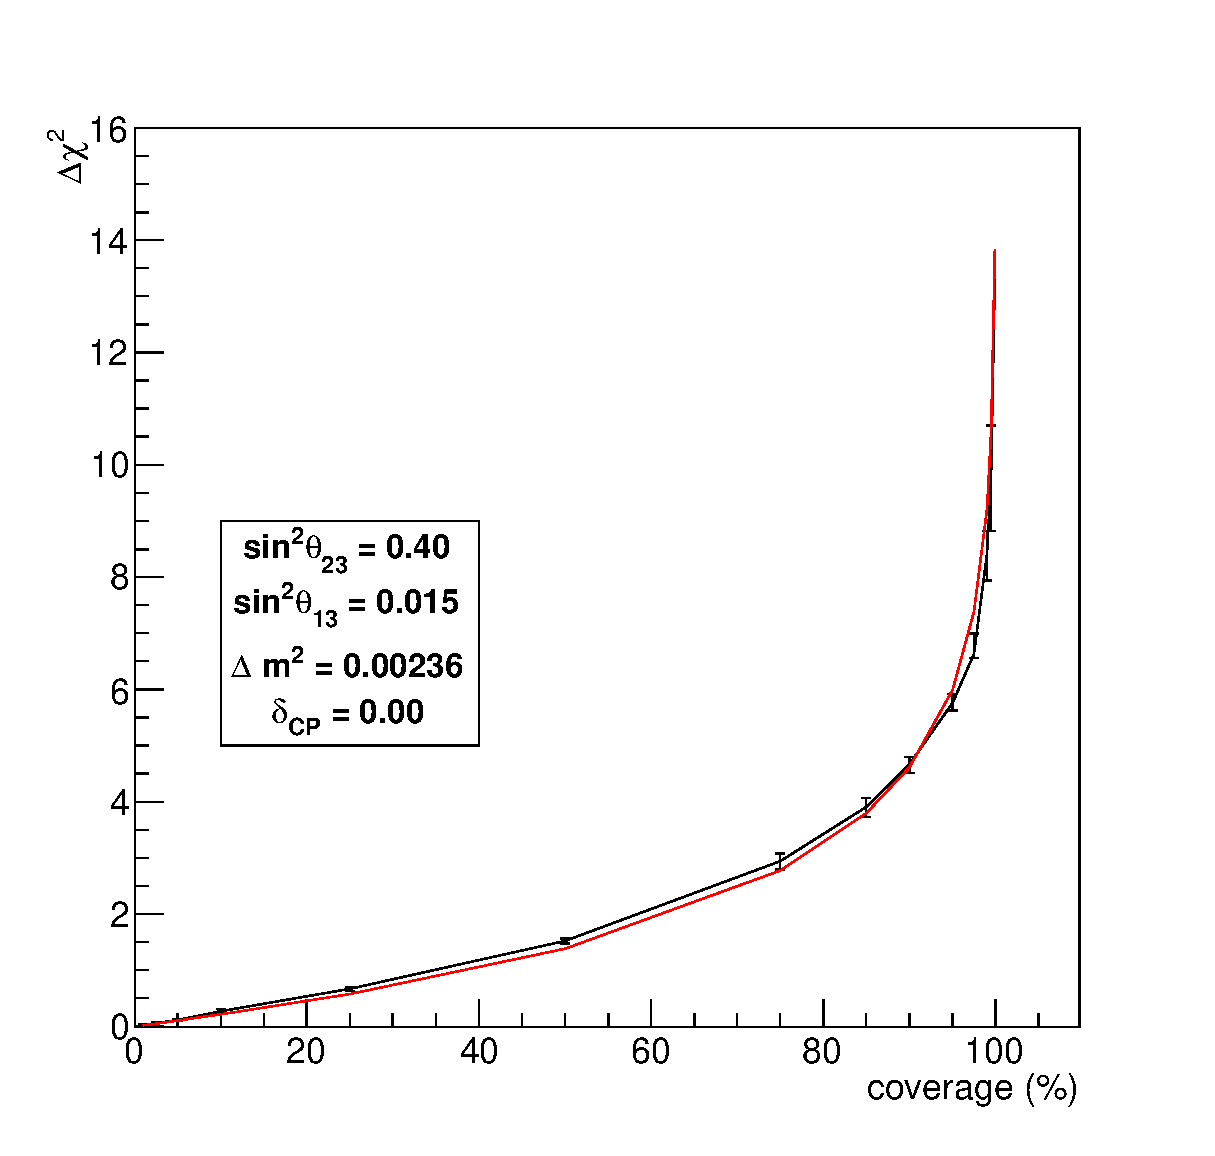
\includegraphics[width=14pc]{./images/appendix/coverage/coverage_study_2D_theta13_theta23_8.eps}
\center
\caption {
  Distribution of $\Delta\chi^{2}$ vs coverage in the ($sin^{2}\theta_{13}$,$sin^{2}\theta_{23}$) parameter space
  from 1k toy MC experiments generated with the Run 1+2+3 POT
  with statistical fluctuations at the oscillation point indicated in the legend. 
}
\label{fig:cov_2D_theta13_theta23_8}
\end{minipage}
\hspace{0.03\linewidth}
\begin{minipage}[t]{0.46\linewidth}
\center
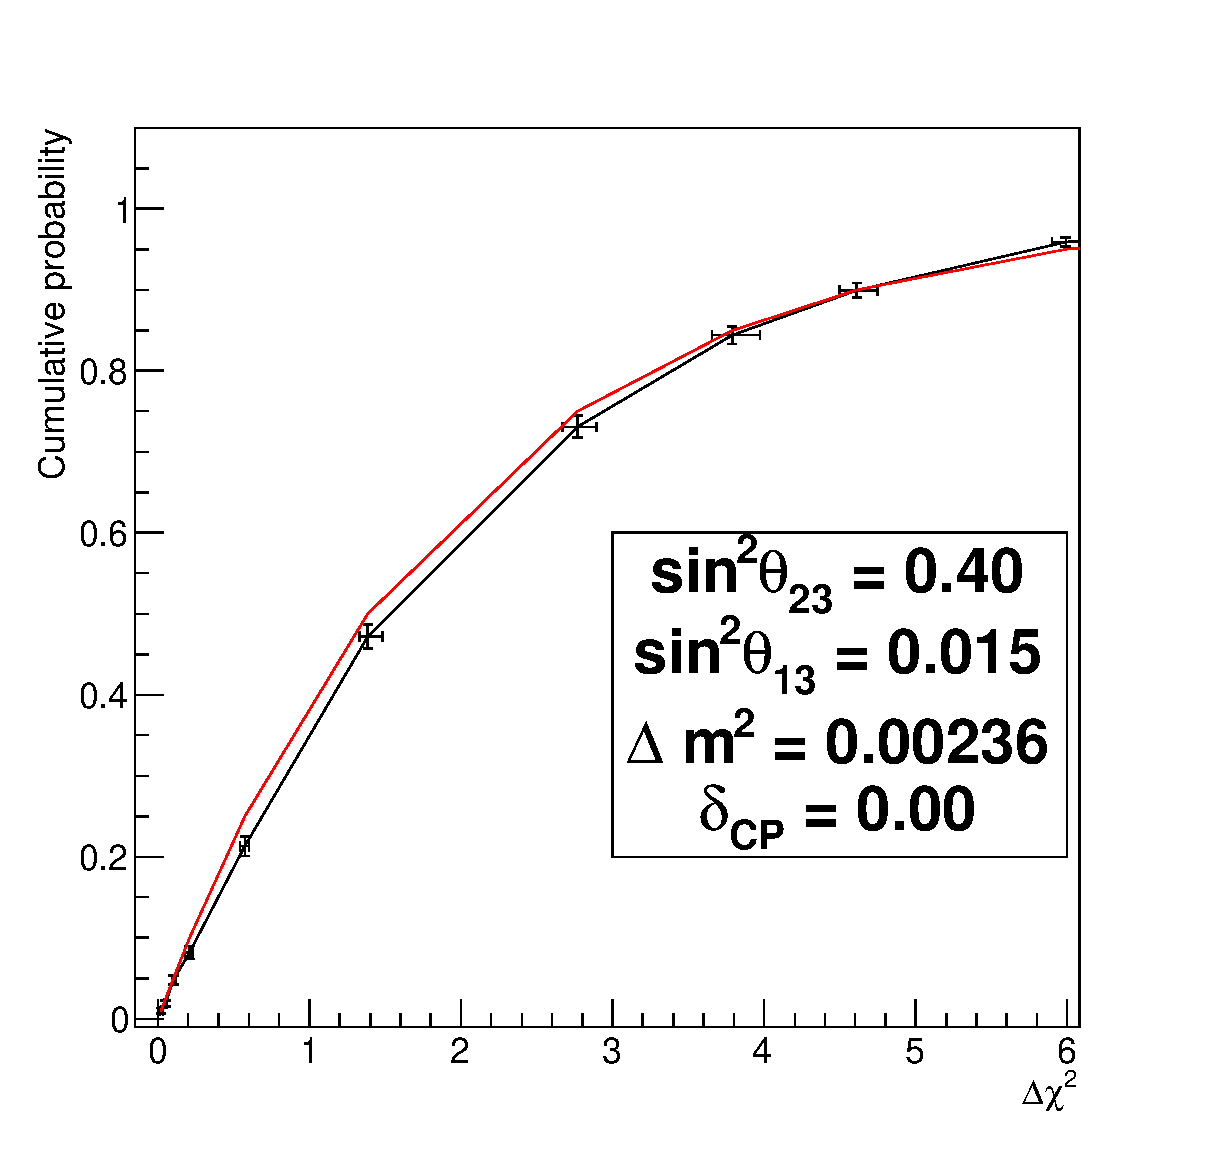
\includegraphics[width=14pc]{./images/appendix/coverage/coverage_study_2D_theta13_theta23_stats_new_8.eps}
\center
\caption {
  Distribution of cumulative probability vs $\Delta\chi^{2}$ in the ($sin^{2}\theta_{13}$,$sin^{2}\theta_{23}$) parameter space
  from 1k toy MC experiments generated with the Run 1+2+3 POT
  with statistical fluctuations at the oscillation point indicated in the legend. 
}
\label{fig:prob_2D_theta13_theta23_8}
\end{minipage}
\end{figure*}
\end{center}


\begin{center}
\begin{figure*}[htb]
\begin{minipage}[t]{0.46\linewidth}
\center
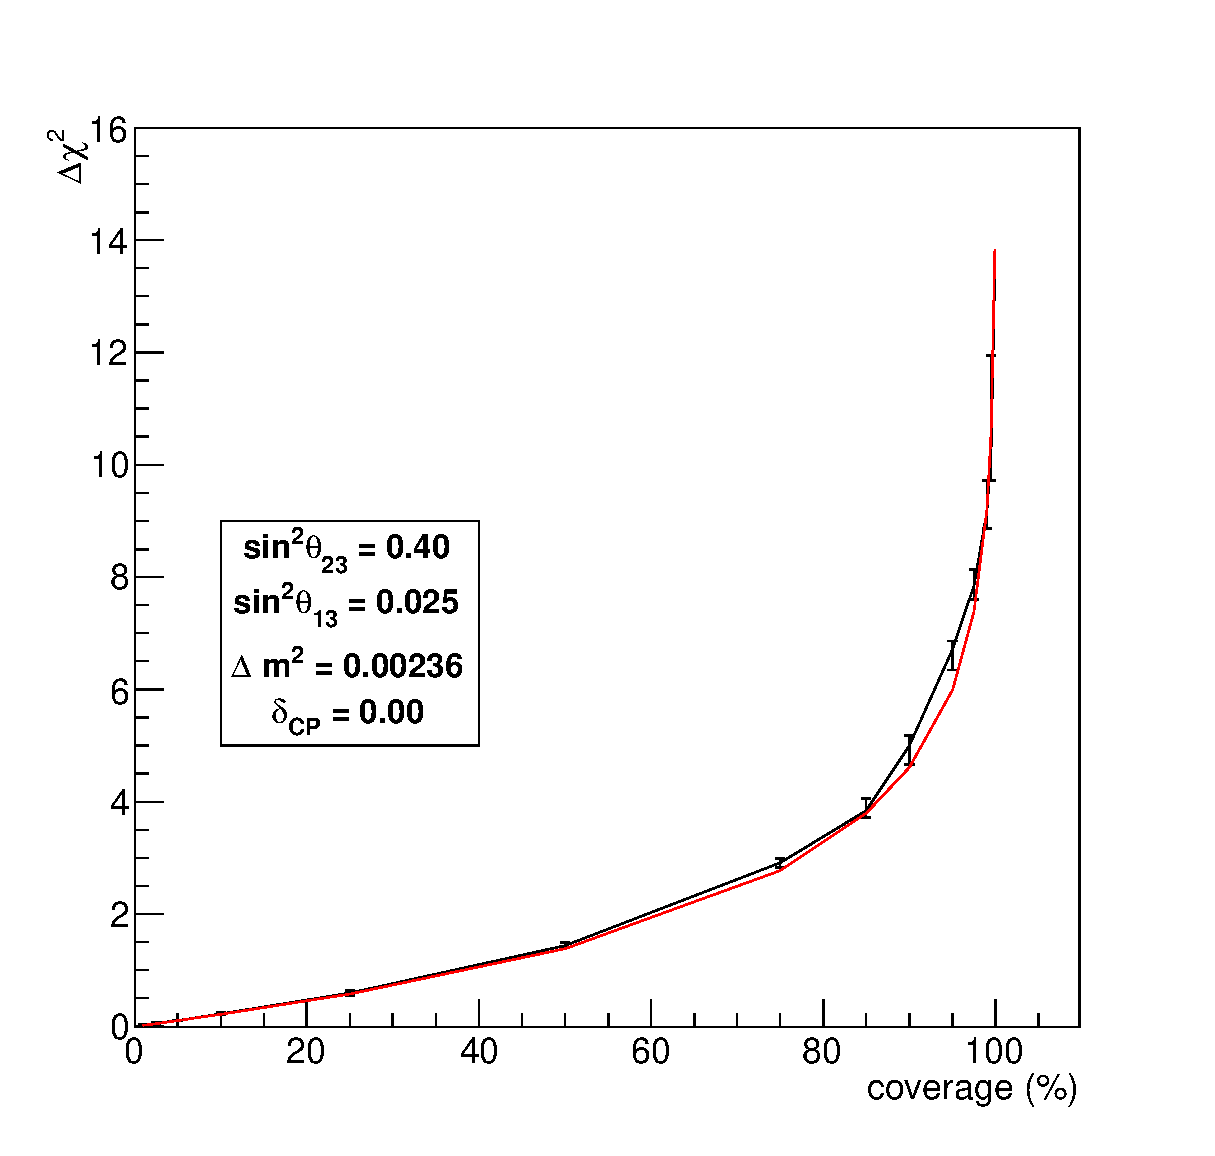
\includegraphics[width=14pc]{./images/appendix/coverage/coverage_study_2D_theta13_theta23_9.eps}
\center
\caption {
  Distribution of $\Delta\chi^{2}$ vs coverage in the ($sin^{2}\theta_{13}$,$sin^{2}\theta_{23}$) parameter space
  from 1k toy MC experiments generated with the Run 1+2+3 POT
  with statistical fluctuations at the oscillation point indicated in the legend. 
}
\label{fig:cov_2D_theta13_theta23_9}
\end{minipage}
\hspace{0.03\linewidth}
\begin{minipage}[t]{0.46\linewidth}
\center
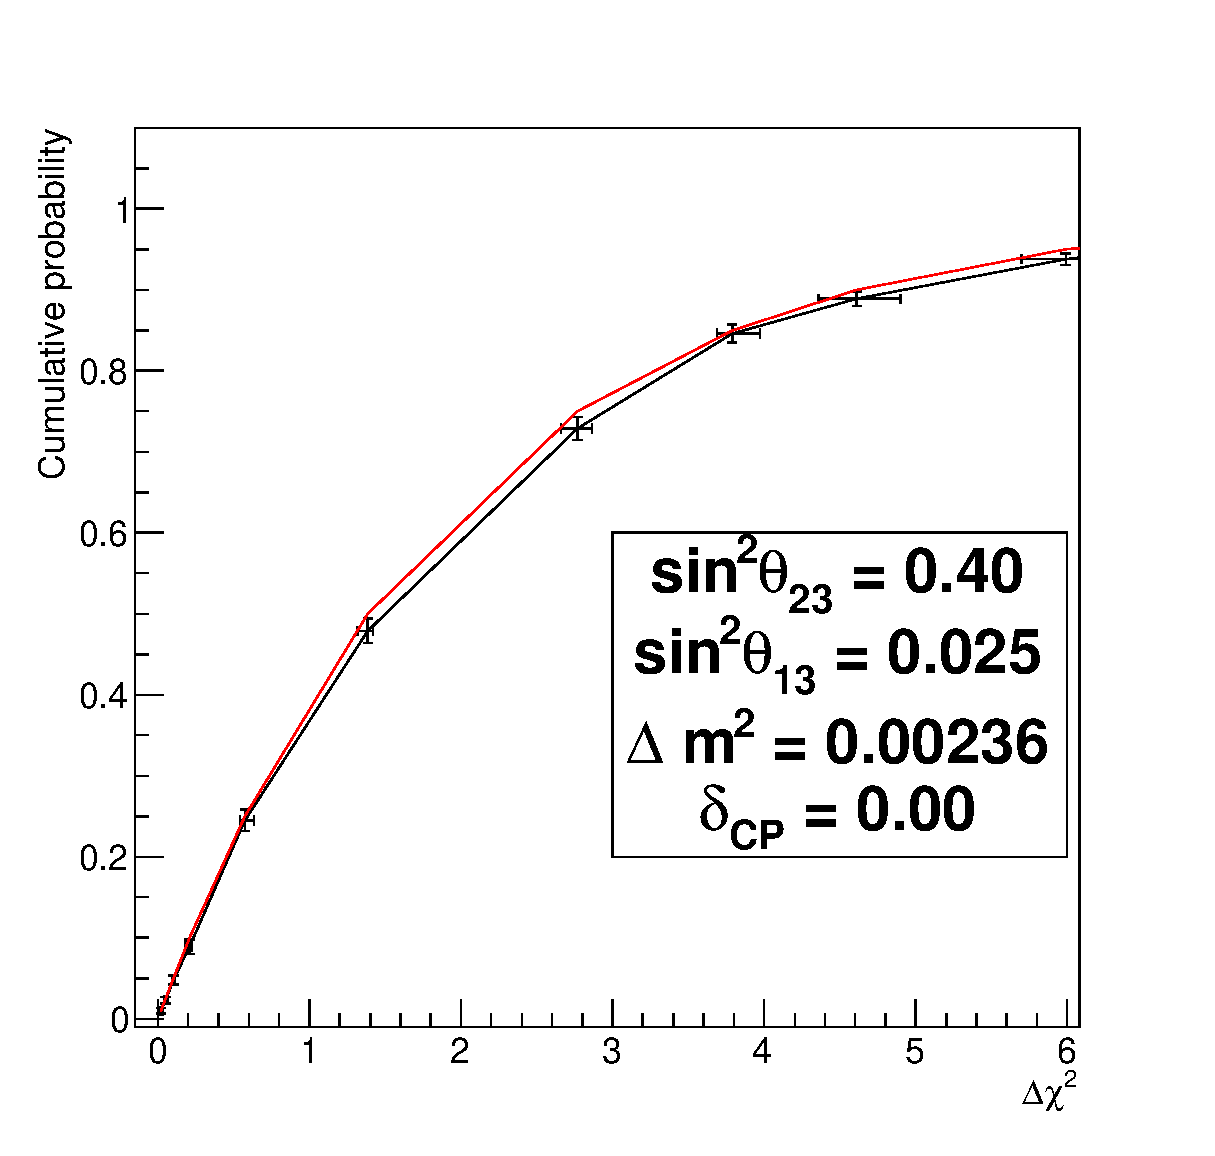
\includegraphics[width=14pc]{./images/appendix/coverage/coverage_study_2D_theta13_theta23_stats_new_9.eps}
\center
\caption {
  Distribution of cumulative probability vs $\Delta\chi^{2}$ in the ($sin^{2}\theta_{13}$,$sin^{2}\theta_{23}$) parameter space
  from 1k toy MC experiments generated with the Run 1+2+3 POT
  with statistical fluctuations at the oscillation point indicated in the legend. 
}
\label{fig:prob_2D_theta13_theta23_9}
\end{minipage}
\vfill
\vspace*{0.7cm}
\begin{minipage}[t]{0.46\linewidth}
\center
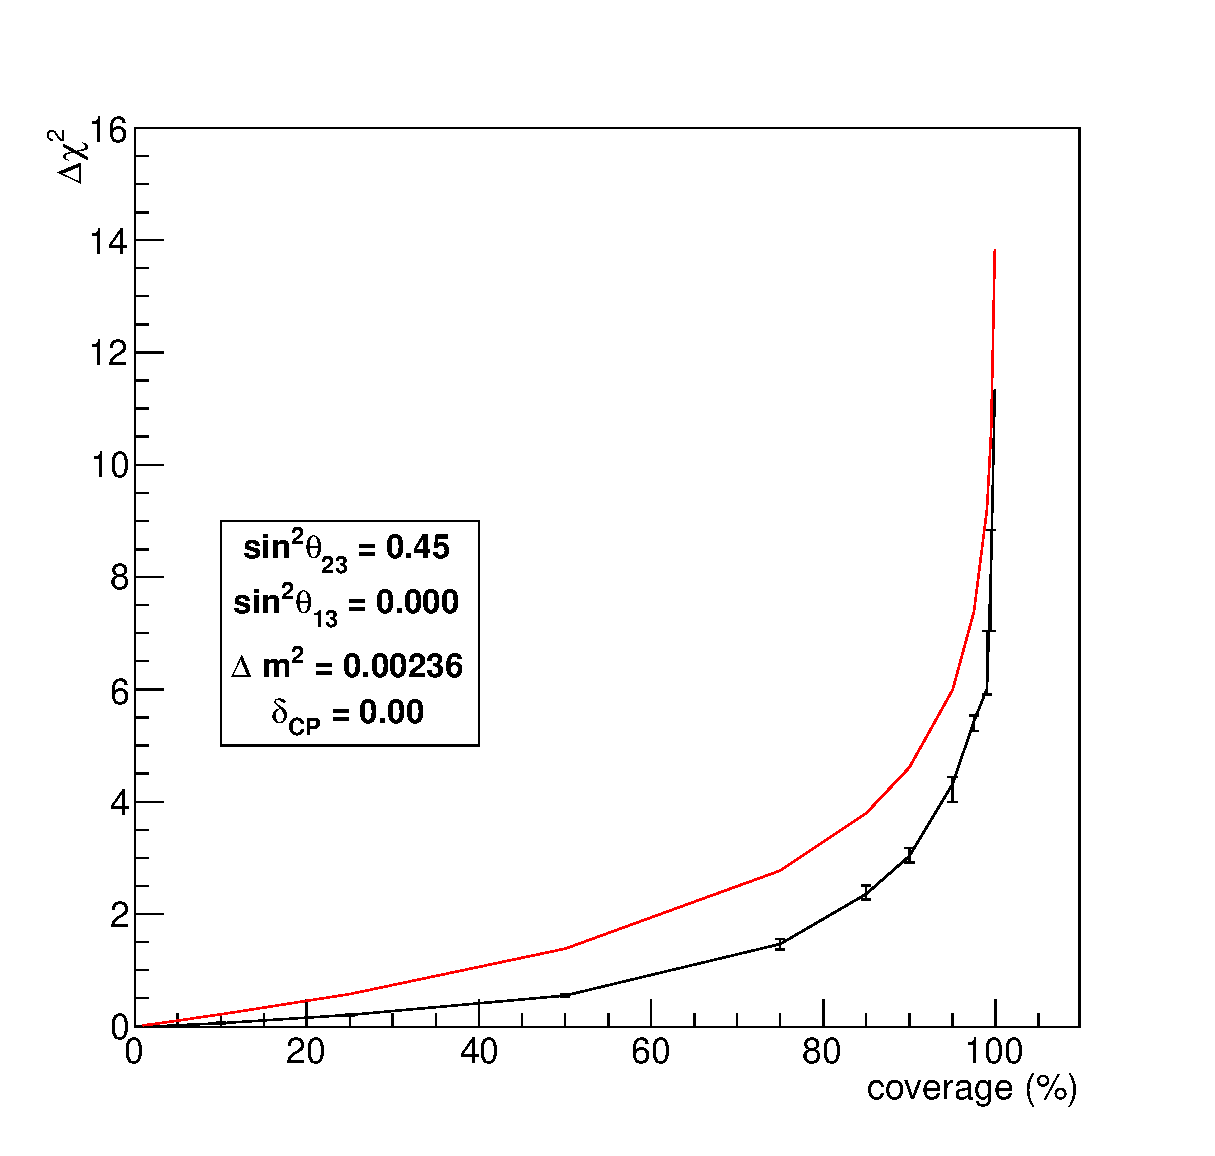
\includegraphics[width=14pc]{./images/appendix/coverage/coverage_study_2D_theta13_theta23_10.eps}
\center
\caption {
  Distribution of $\Delta\chi^{2}$ vs coverage in the ($sin^{2}\theta_{13}$,$sin^{2}\theta_{23}$) parameter space
  from 1k toy MC experiments generated with the Run 1+2+3 POT
  with statistical fluctuations at the oscillation point indicated in the legend. 
}
\label{fig:cov_2D_theta13_theta23_10}
\end{minipage}
\hspace{0.03\linewidth}
\begin{minipage}[t]{0.46\linewidth}
\center
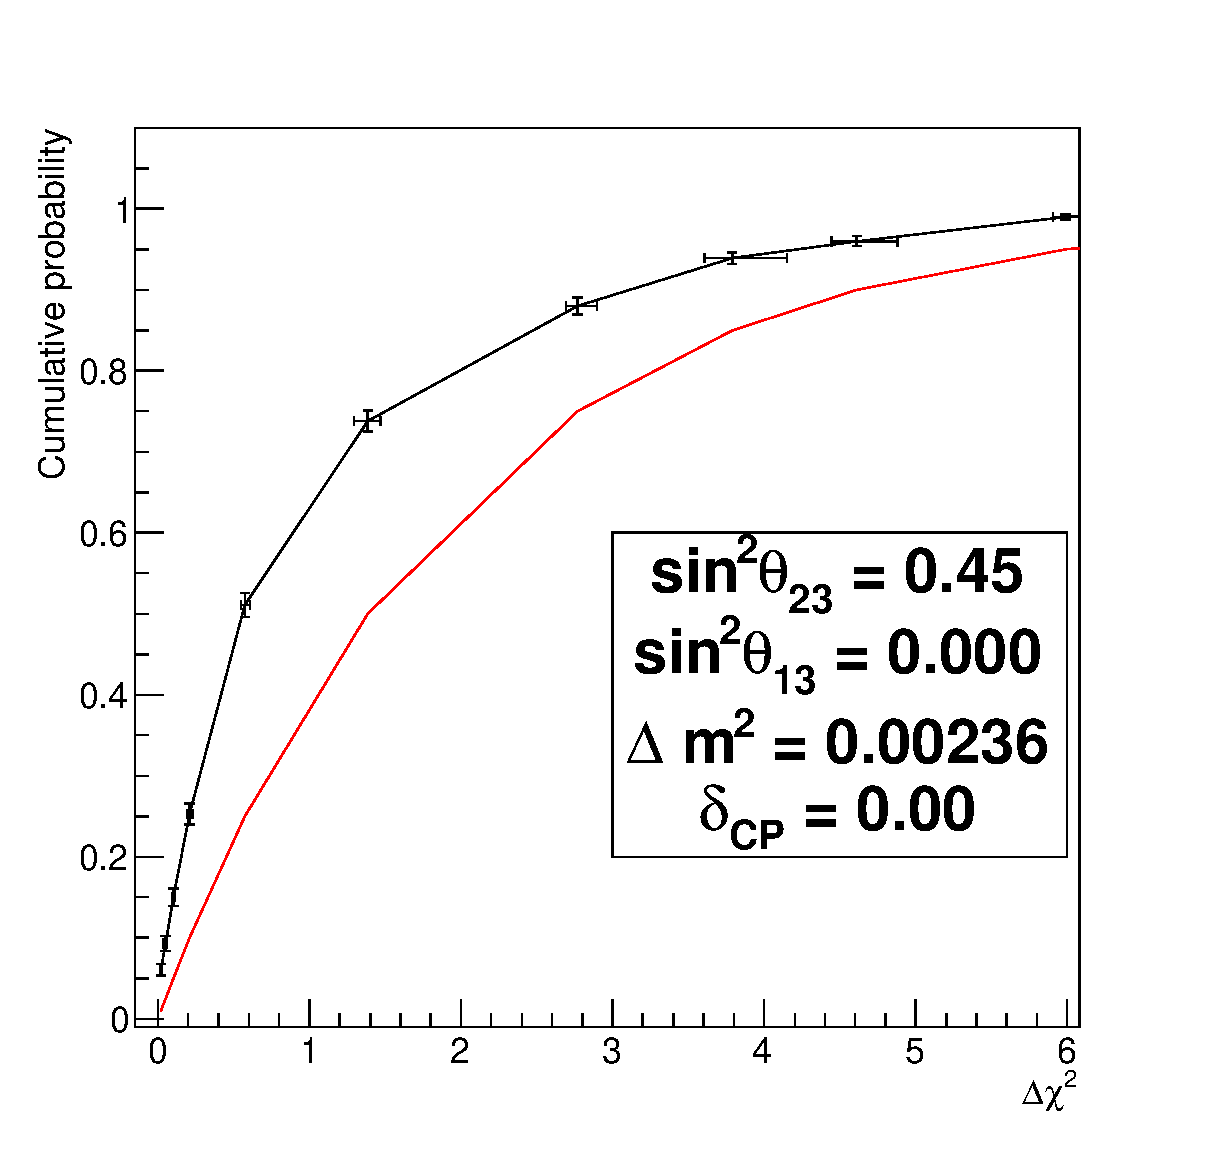
\includegraphics[width=14pc]{./images/appendix/coverage/coverage_study_2D_theta13_theta23_stats_new_10.eps}
\center
\caption {
  Distribution of cumulative probability vs $\Delta\chi^{2}$ in the ($sin^{2}\theta_{13}$,$sin^{2}\theta_{23}$) parameter space
  from 1k toy MC experiments generated with the Run 1+2+3 POT
  with statistical fluctuations at the oscillation point indicated in the legend. 
}
\label{fig:prob_2D_theta13_theta23_10}
\end{minipage}
\vfill
\vspace*{0.7cm}
\begin{minipage}[t]{0.46\linewidth}
\center
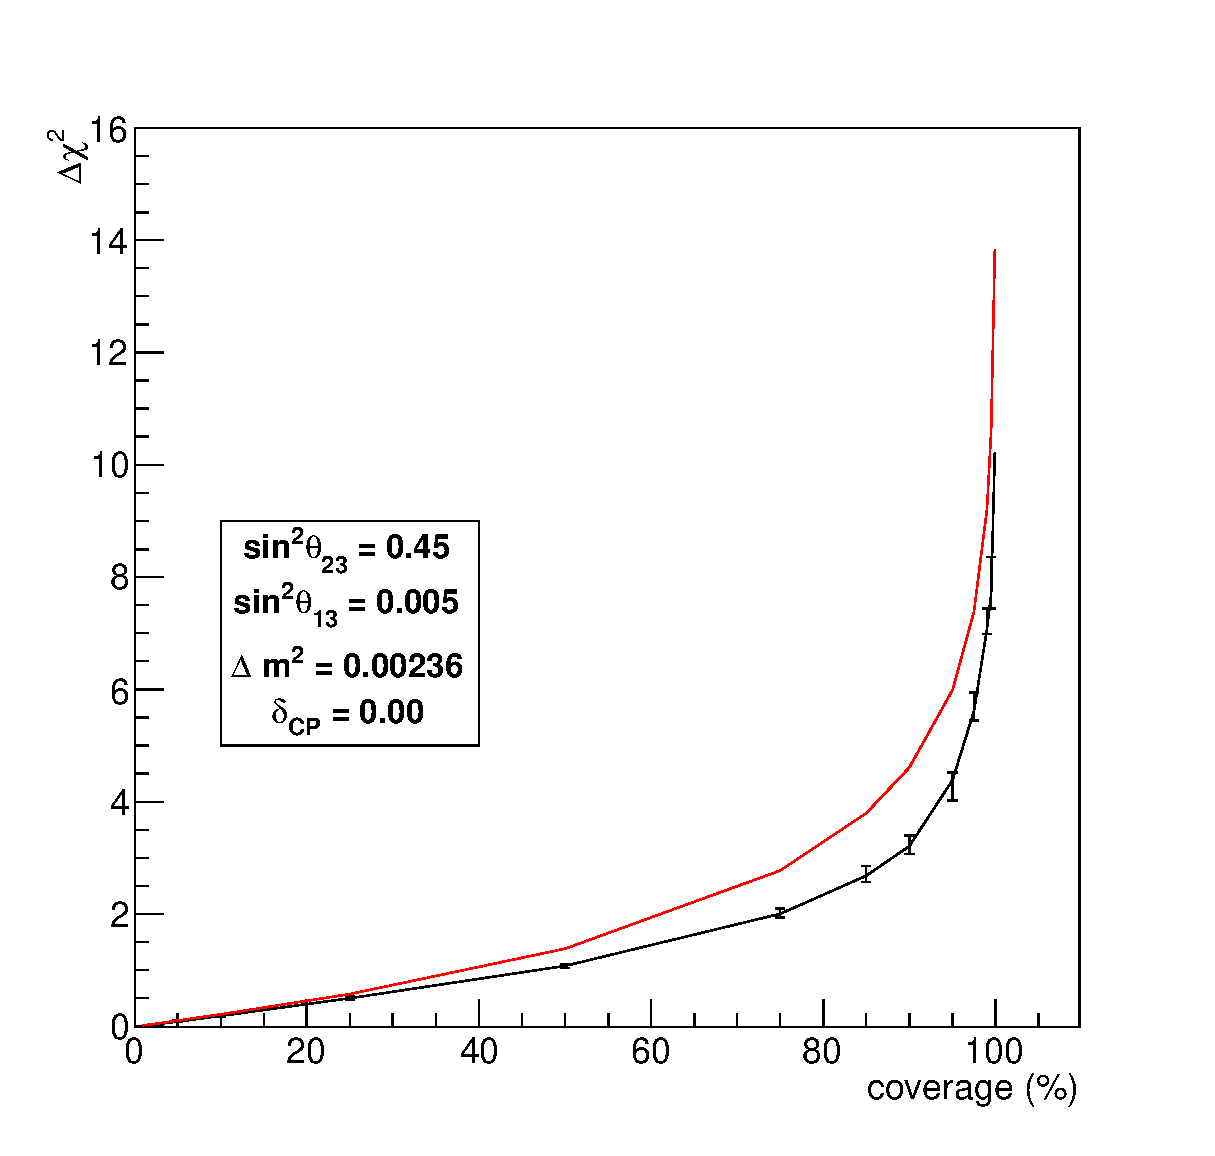
\includegraphics[width=14pc]{./images/appendix/coverage/coverage_study_2D_theta13_theta23_11.eps}
\center
\caption {
  Distribution of $\Delta\chi^{2}$ vs coverage in the ($sin^{2}\theta_{13}$,$sin^{2}\theta_{23}$) parameter space
  from 1k toy MC experiments generated with the Run 1+2+3 POT
  with statistical fluctuations at the oscillation point indicated in the legend. 
}
\label{fig:cov_2D_theta13_theta23_11}
\end{minipage}
\hspace{0.03\linewidth}
\begin{minipage}[t]{0.46\linewidth}
\center
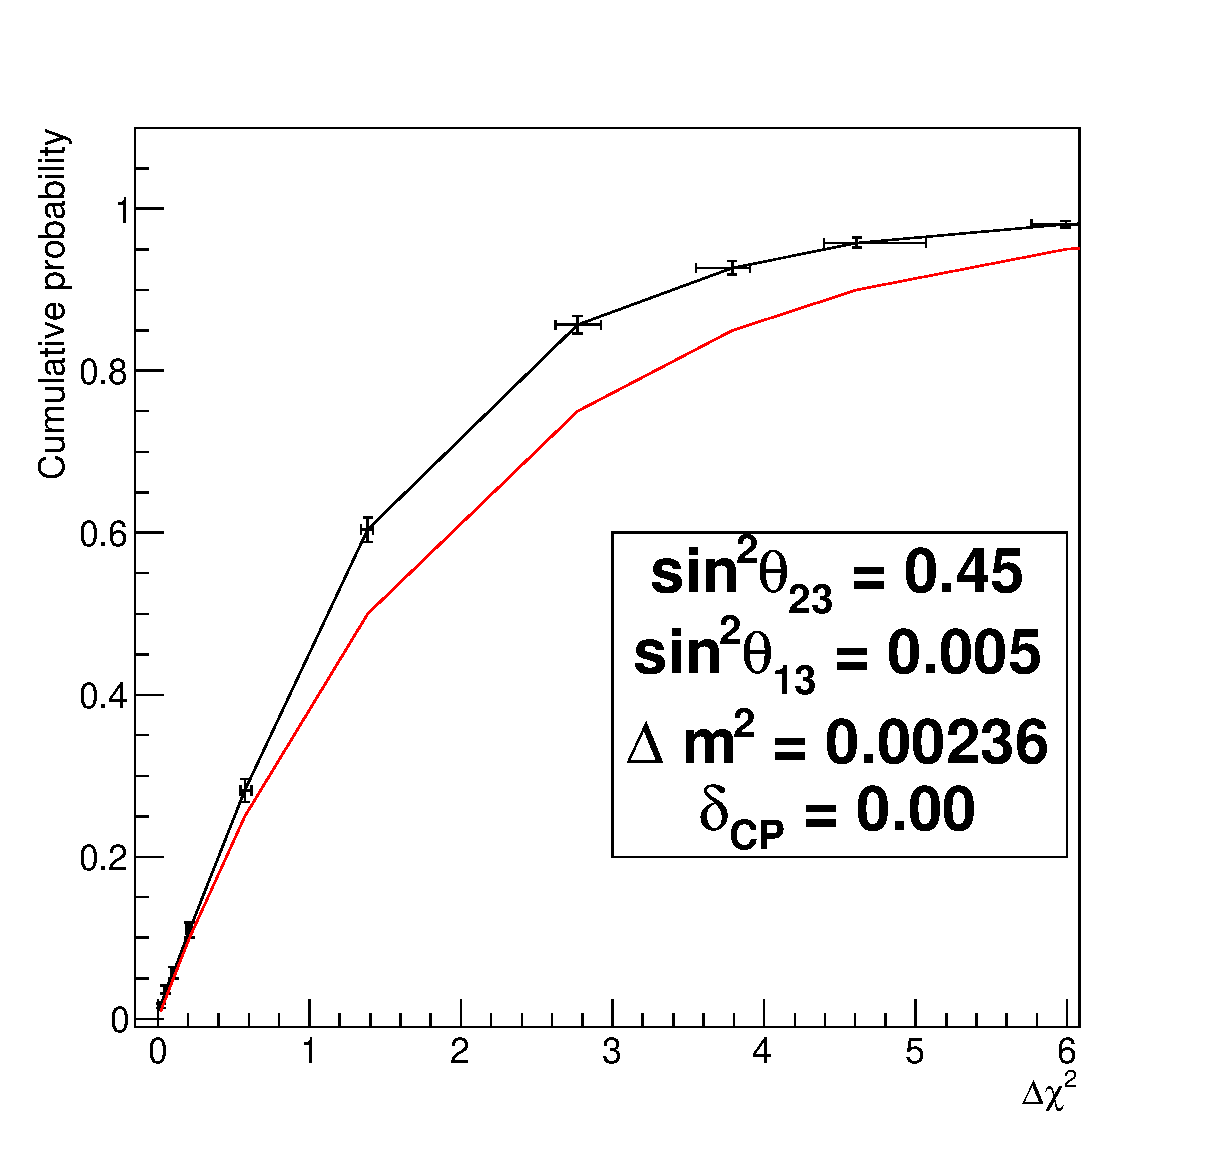
\includegraphics[width=14pc]{./images/appendix/coverage/coverage_study_2D_theta13_theta23_stats_new_11.eps}
\center
\caption {
  Distribution of cumulative probability vs $\Delta\chi^{2}$ in the ($sin^{2}\theta_{13}$,$sin^{2}\theta_{23}$) parameter space
  from 1k toy MC experiments generated with the Run 1+2+3 POT
  with statistical fluctuations at the oscillation point indicated in the legend. 
}
\label{fig:prob_2D_theta13_theta23_11}
\end{minipage}
\end{figure*}
\end{center}

\begin{center}
\begin{figure*}[htb]
\begin{minipage}[t]{0.46\linewidth}
\center
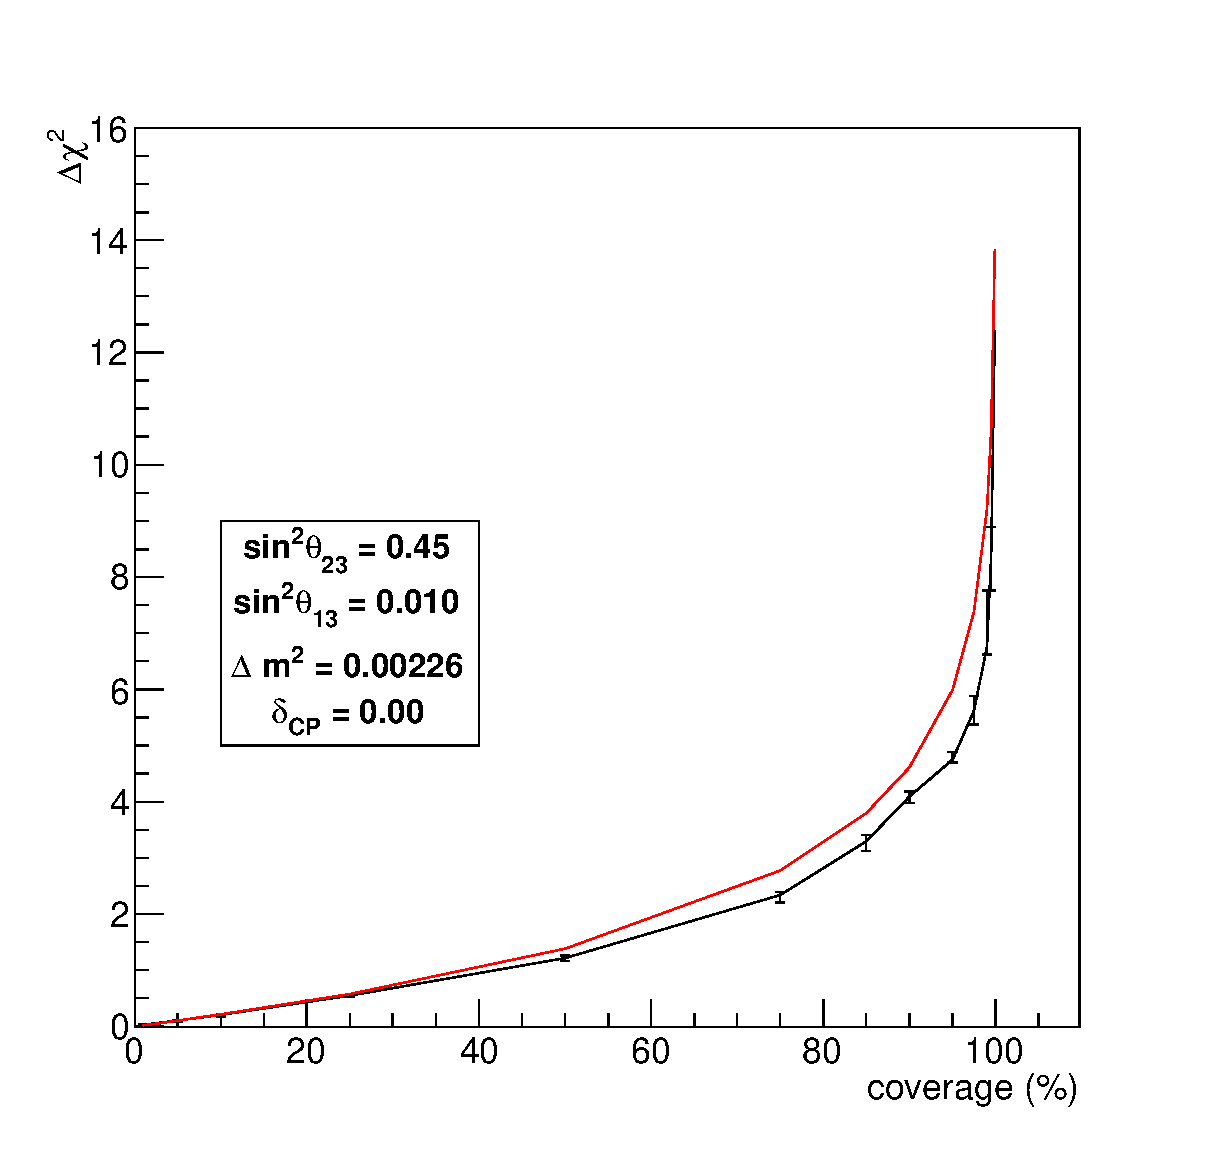
\includegraphics[width=14pc]{./images/appendix/coverage/coverage_study_2D_theta13_theta23_12.eps}
\center
\caption {
  Distribution of $\Delta\chi^{2}$ vs coverage in the ($sin^{2}\theta_{13}$,$sin^{2}\theta_{23}$) parameter space
  from 1k toy MC experiments generated with the Run 1+2+3 POT
  with statistical fluctuations at the oscillation point indicated in the legend. 
}
\label{fig:cov_2D_theta13_theta23_12}
\end{minipage}
\hspace{0.03\linewidth}
\begin{minipage}[t]{0.46\linewidth}
\center
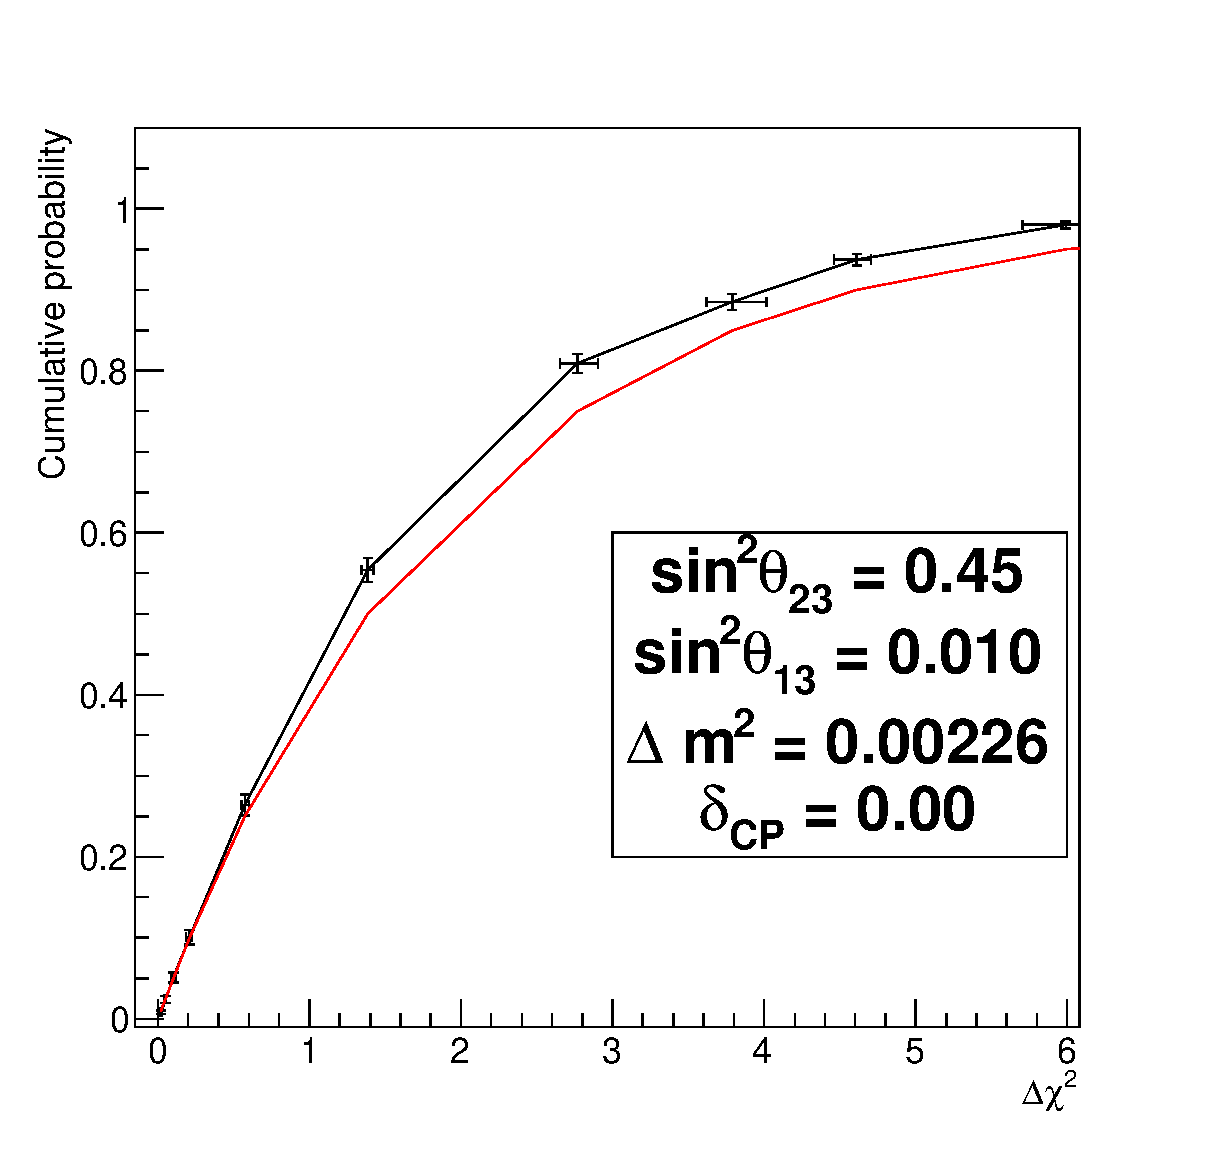
\includegraphics[width=14pc]{./images/appendix/coverage/coverage_study_2D_theta13_theta23_stats_new_12.eps}
\center
\caption {
  Distribution of cumulative probability vs $\Delta\chi^{2}$ in the ($sin^{2}\theta_{13}$,$sin^{2}\theta_{23}$) parameter space
  from 1k toy MC experiments generated with the Run 1+2+3 POT
  with statistical fluctuations at the oscillation point indicated in the legend. 
}
\label{fig:prob_2D_theta13_theta23_12}
\end{minipage}
\vfill
\vspace*{0.7cm}
\begin{minipage}[t]{0.46\linewidth}
\center
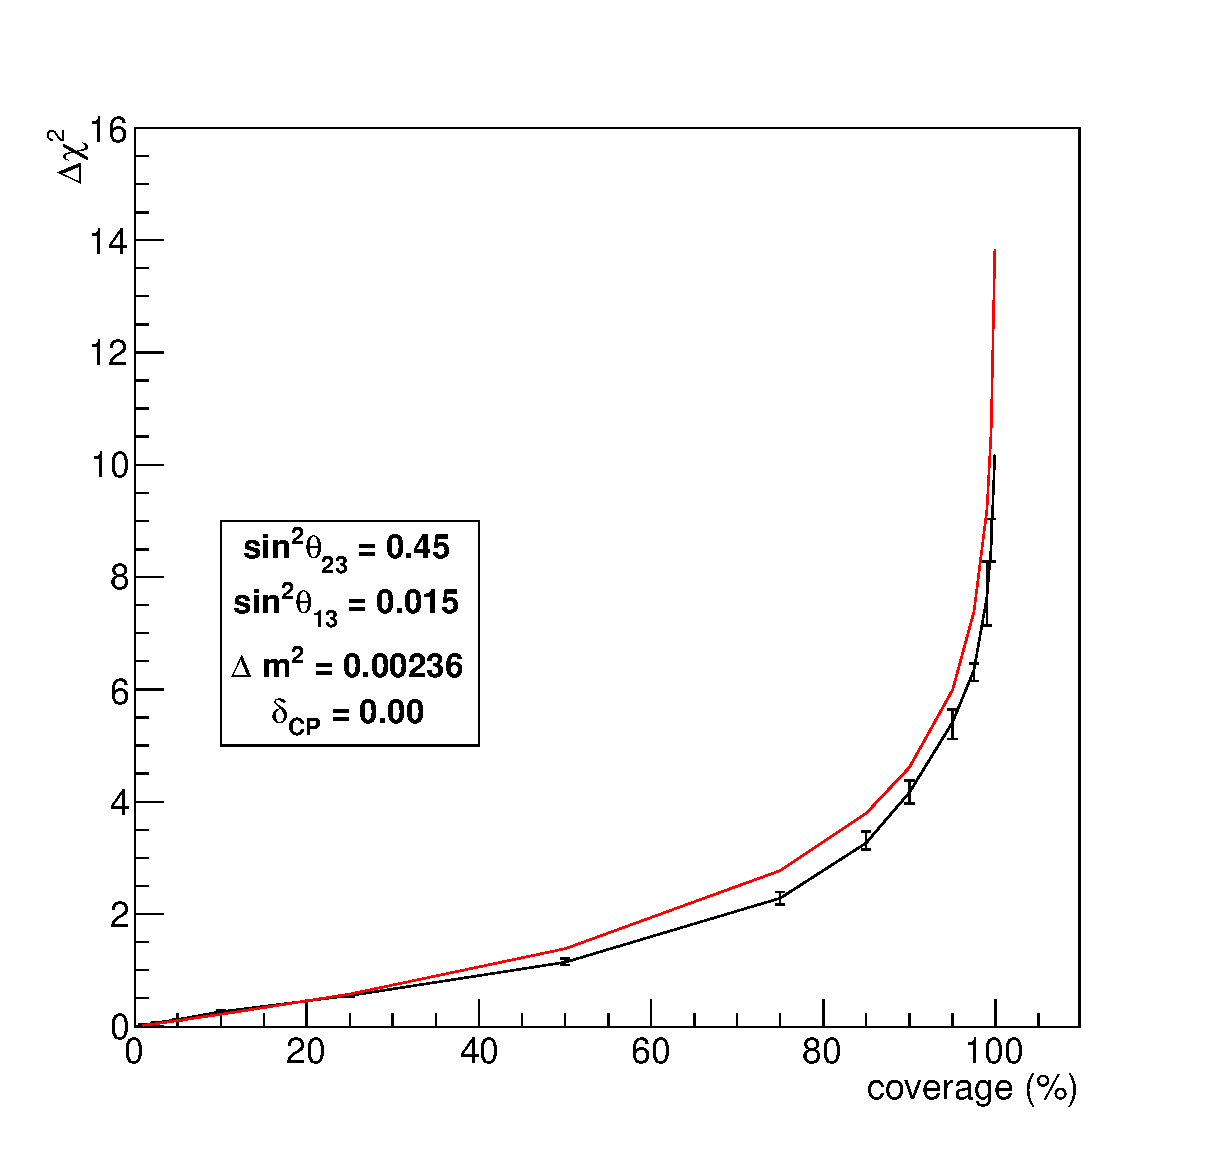
\includegraphics[width=14pc]{./images/appendix/coverage/coverage_study_2D_theta13_theta23_13.eps}
\center
\caption {
  Distribution of $\Delta\chi^{2}$ vs coverage in the ($sin^{2}\theta_{13}$,$sin^{2}\theta_{23}$) parameter space
  from 1k toy MC experiments generated with the Run 1+2+3 POT
  with statistical fluctuations at the oscillation point indicated in the legend. 
}
\label{fig:cov_2D_theta13_theta23_13}
\end{minipage}
\hspace{0.03\linewidth}
\begin{minipage}[t]{0.46\linewidth}
\center
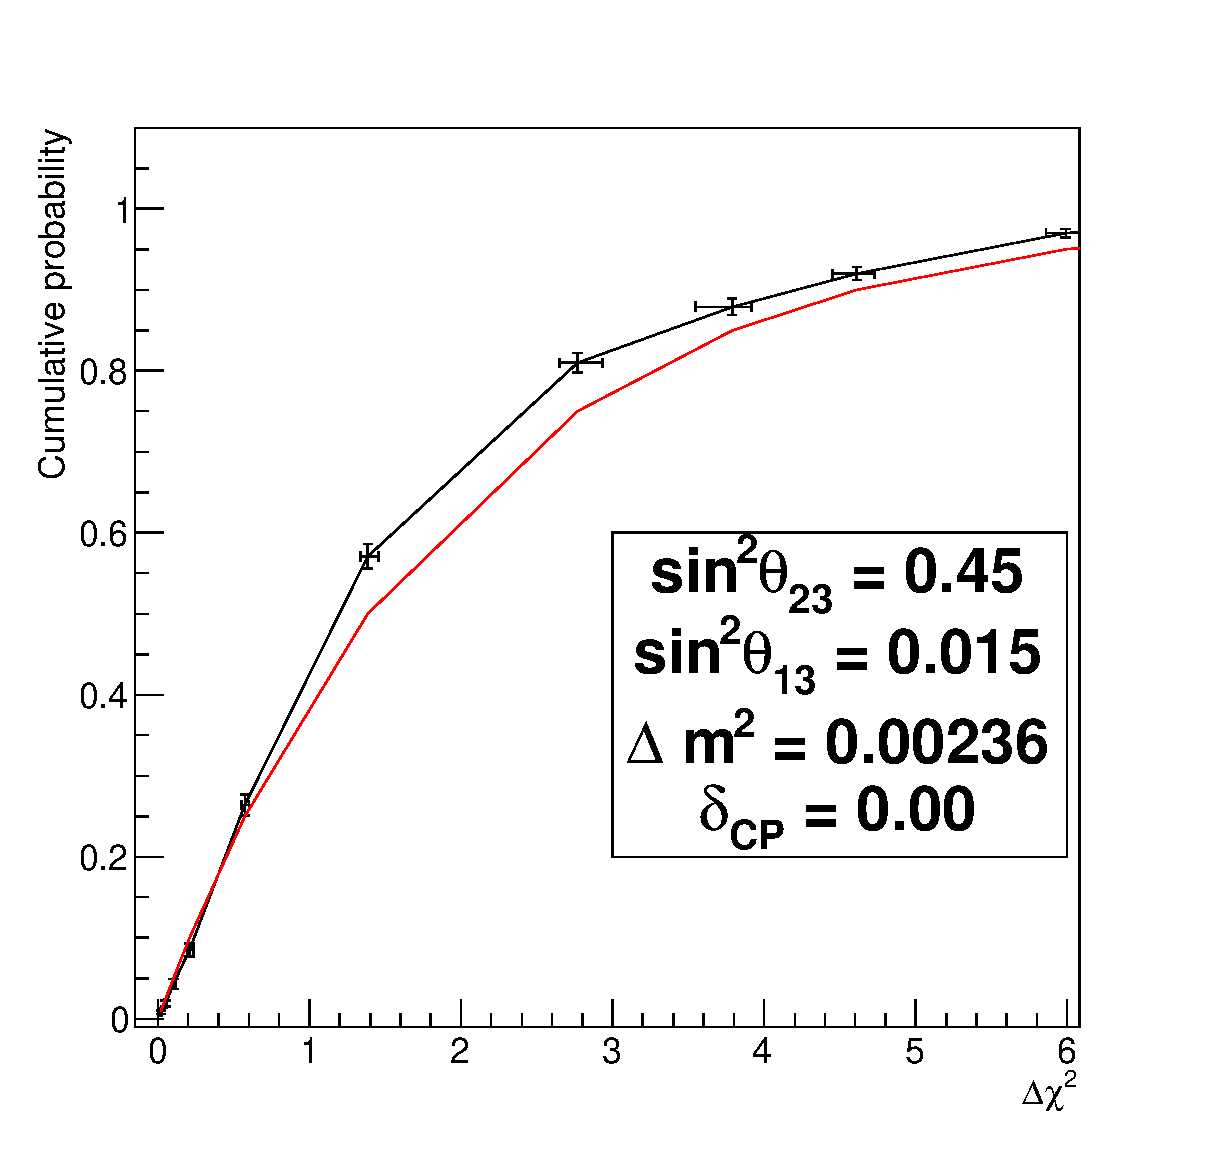
\includegraphics[width=14pc]{./images/appendix/coverage/coverage_study_2D_theta13_theta23_stats_new_13.eps}
\center
\caption {
  Distribution of cumulative probability vs $\Delta\chi^{2}$ in the ($sin^{2}\theta_{13}$,$sin^{2}\theta_{23}$) parameter space
  from 1k toy MC experiments generated with the Run 1+2+3 POT
  with statistical fluctuations at the oscillation point indicated in the legend. 
}
\label{fig:prob_2D_theta13_theta23_13}
\end{minipage}
\vfill
\vspace*{0.7cm}
\begin{minipage}[t]{0.46\linewidth}
\center
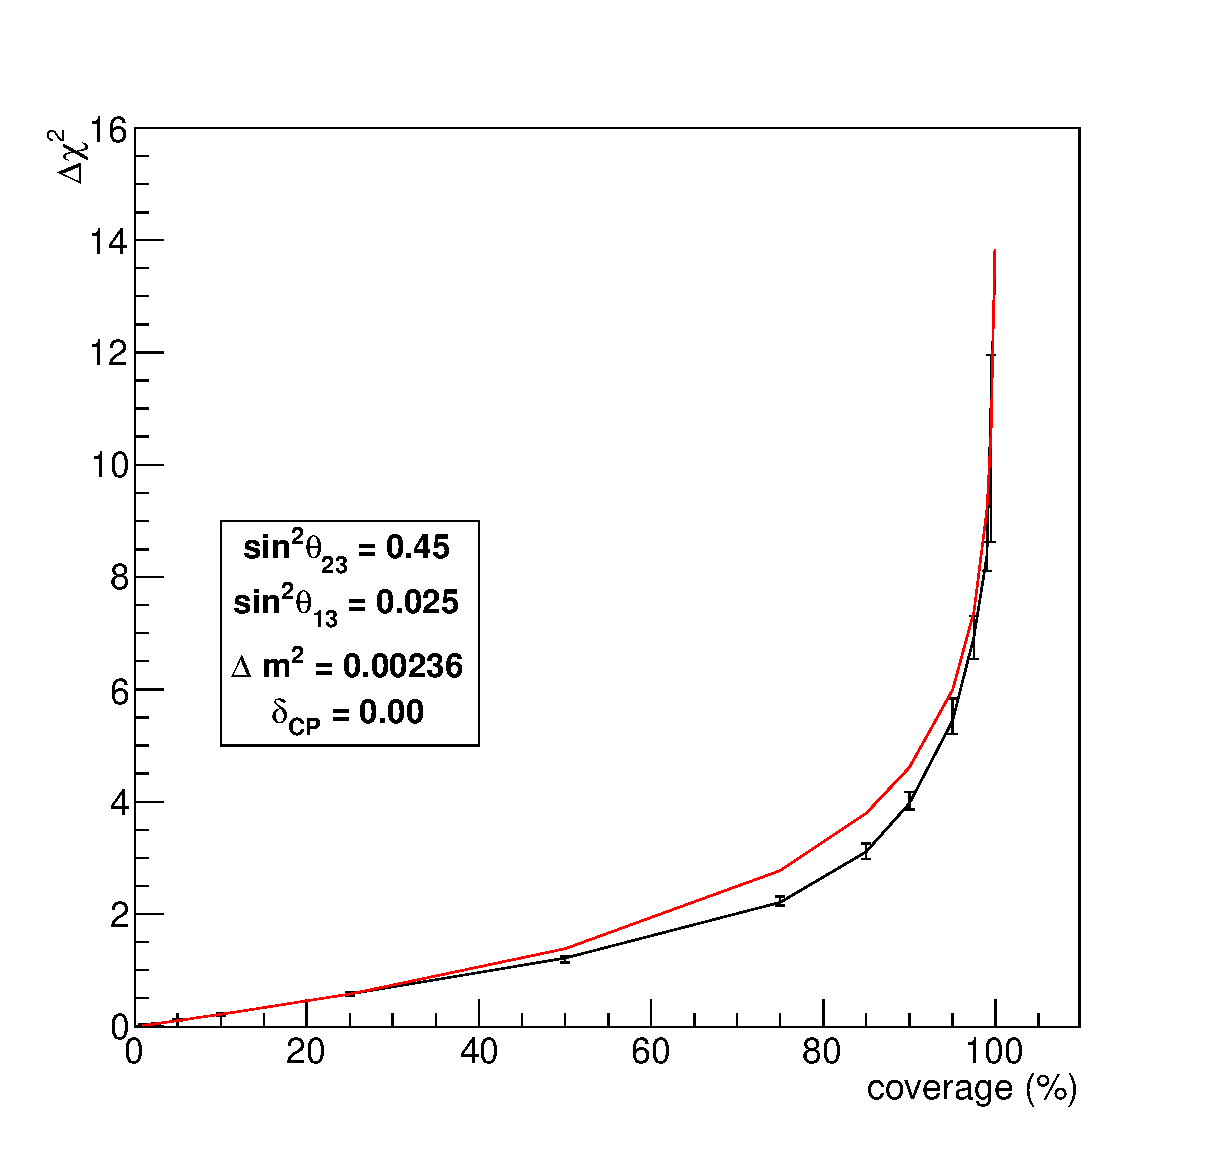
\includegraphics[width=14pc]{./images/appendix/coverage/coverage_study_2D_theta13_theta23_14.eps}
\center
\caption {
  Distribution of $\Delta\chi^{2}$ vs coverage in the ($sin^{2}\theta_{13}$,$sin^{2}\theta_{23}$) parameter space
  from 1k toy MC experiments generated with the Run 1+2+3 POT
  with statistical fluctuations at the oscillation point indicated in the legend. 
}
\label{fig:cov_2D_theta13_theta23_14}
\end{minipage}
\hspace{0.03\linewidth}
\begin{minipage}[t]{0.46\linewidth}
\center
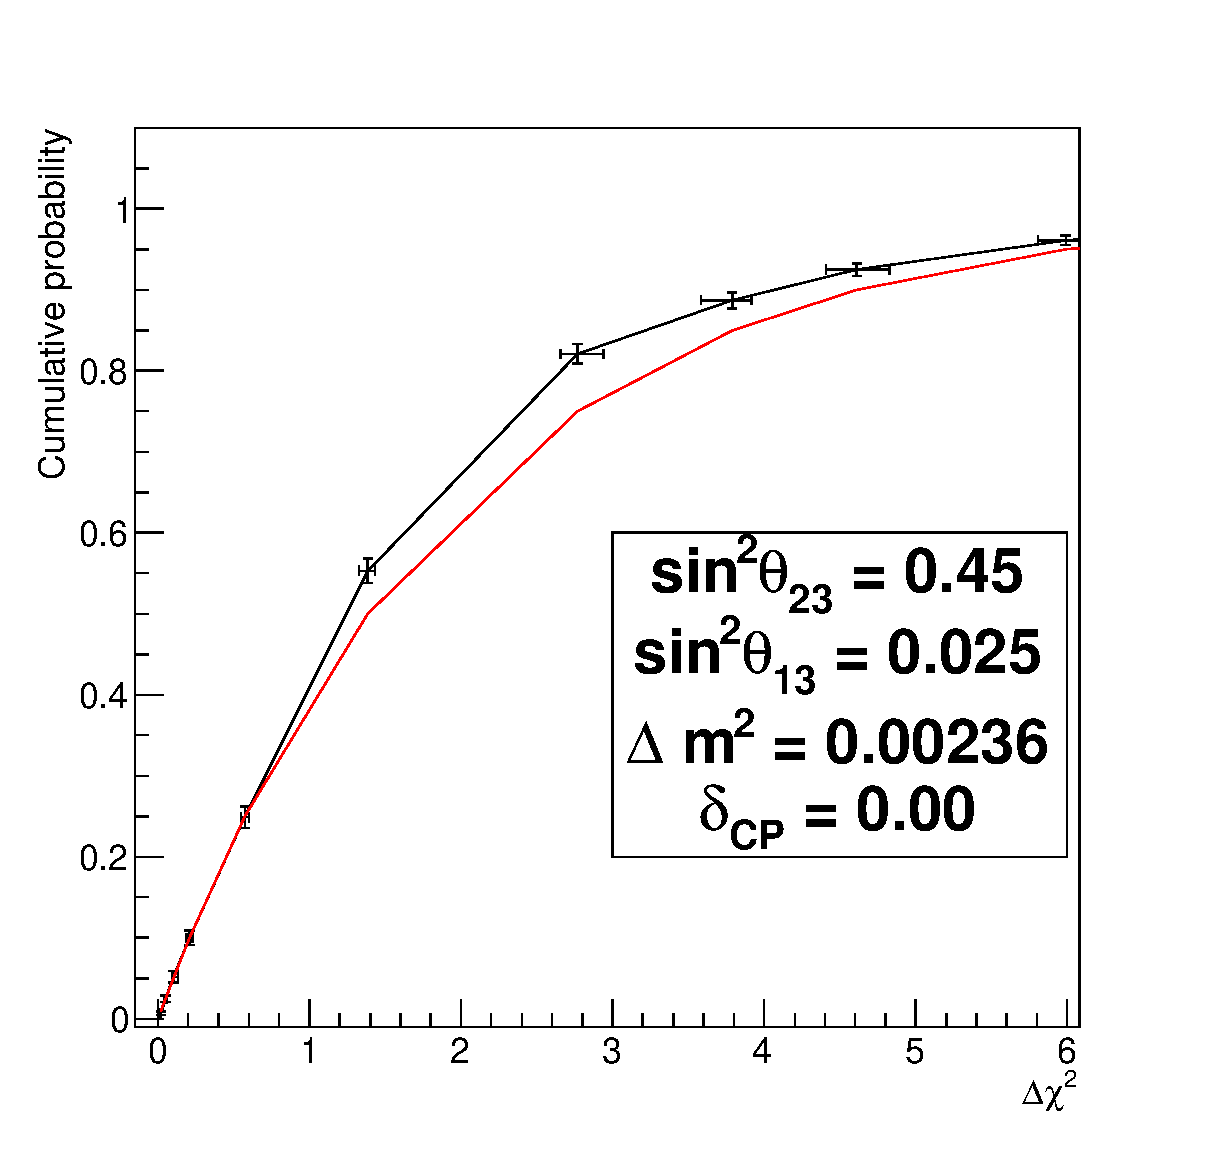
\includegraphics[width=14pc]{./images/appendix/coverage/coverage_study_2D_theta13_theta23_stats_new_14.eps}
\center
\caption {
  Distribution of cumulative probability vs $\Delta\chi^{2}$ in the ($sin^{2}\theta_{13}$,$sin^{2}\theta_{23}$) parameter space
  from 1k toy MC experiments generated with the Run 1+2+3 POT
  with statistical fluctuations at the oscillation point indicated in the legend. 
}
\label{fig:prob_2D_theta13_theta23_14}
\end{minipage}
\end{figure*}
\end{center}

\begin{center}
\begin{figure*}[htb]
\begin{minipage}[t]{0.46\linewidth}
\center
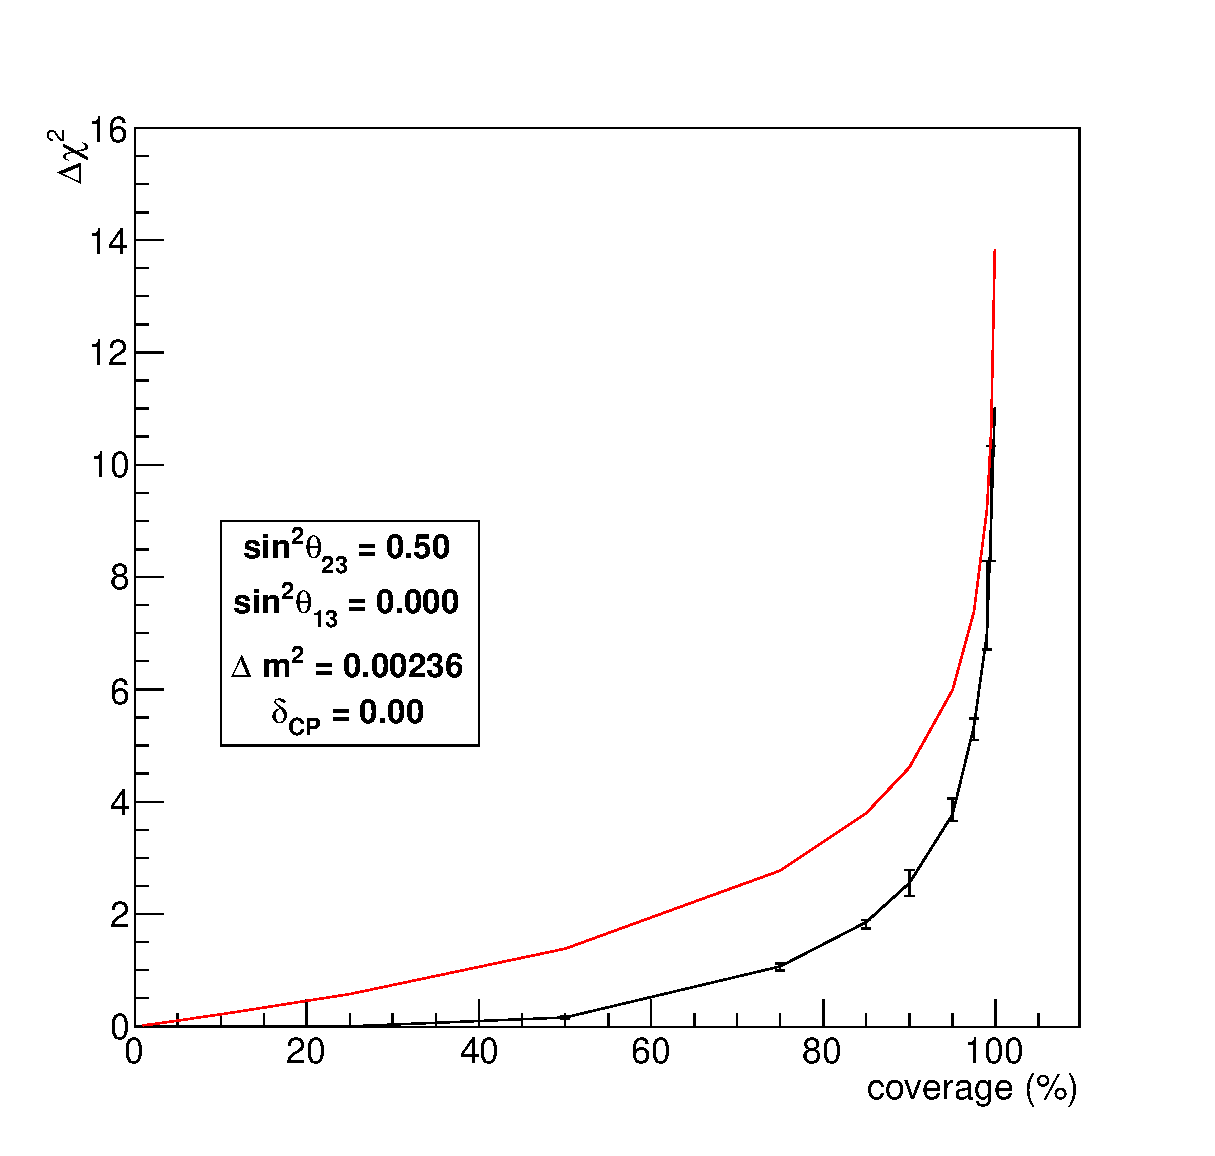
\includegraphics[width=14pc]{./images/appendix/coverage/coverage_study_2D_theta13_theta23_15.eps}
\center
\caption {
  Distribution of $\Delta\chi^{2}$ vs coverage in the ($sin^{2}\theta_{13}$,$sin^{2}\theta_{23}$) parameter space
  from 1k toy MC experiments generated with the Run 1+2+3 POT
  with statistical fluctuations at the oscillation point indicated in the legend. 
}
\label{fig:cov_2D_theta13_theta23_15}
\end{minipage}
\hspace{0.03\linewidth}
\begin{minipage}[t]{0.46\linewidth}
\center
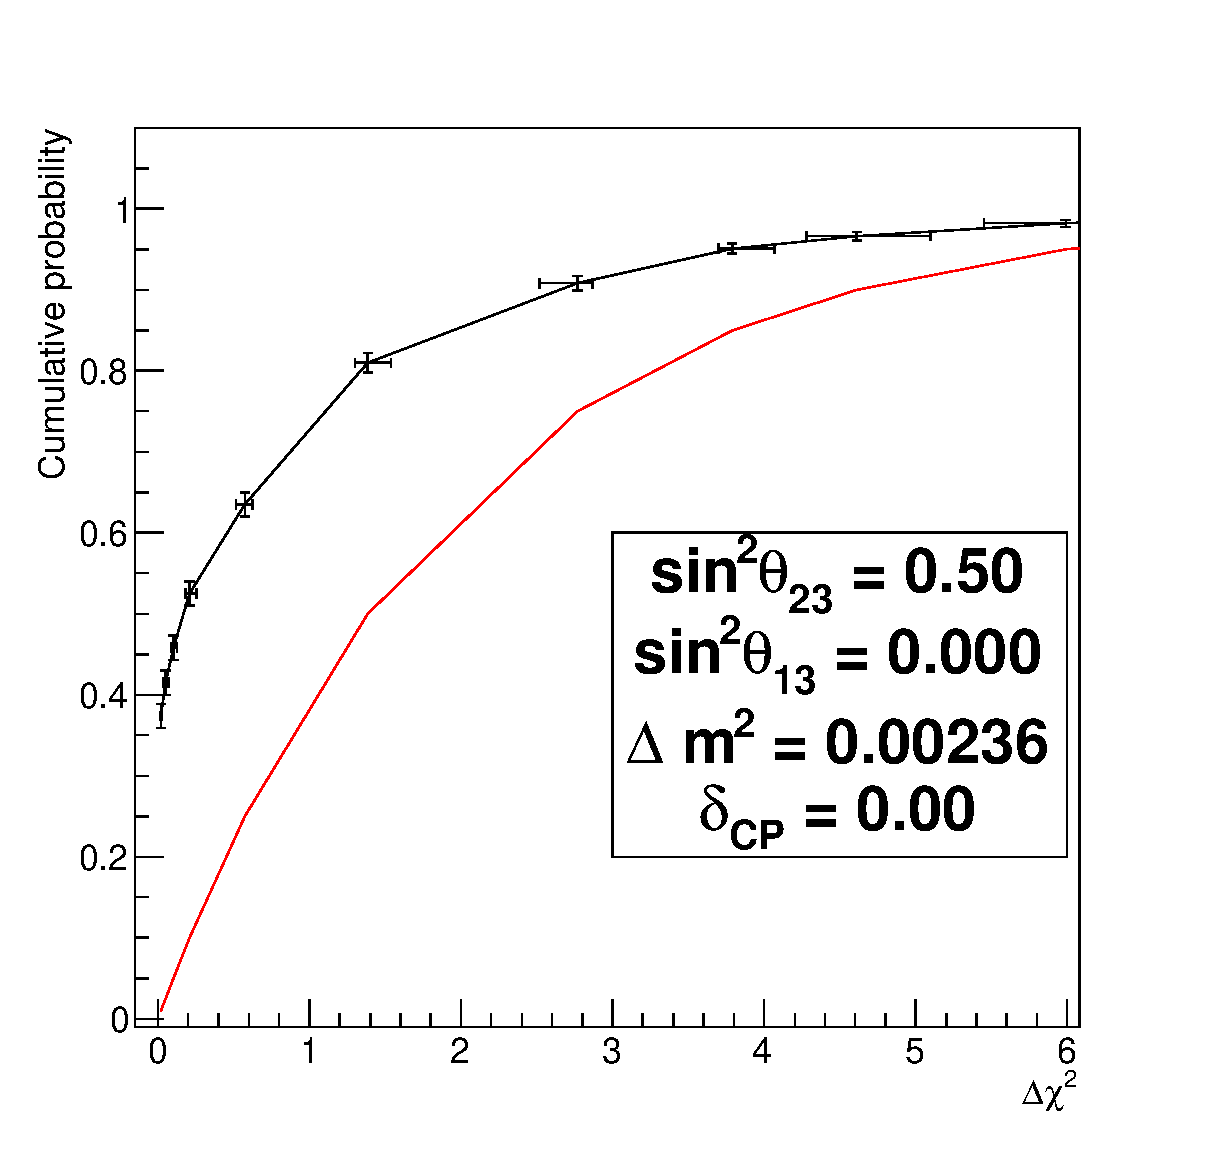
\includegraphics[width=14pc]{./images/appendix/coverage/coverage_study_2D_theta13_theta23_stats_new_15.eps}
\center
\caption {
  Distribution of cumulative probability vs $\Delta\chi^{2}$ in the ($sin^{2}\theta_{13}$,$sin^{2}\theta_{23}$) parameter space
  from 1k toy MC experiments generated with the Run 1+2+3 POT
  with statistical fluctuations at the oscillation point indicated in the legend. 
}
\label{fig:prob_2D_theta13_theta23_15}
\end{minipage}
\vfill
\vspace*{0.7cm}
\begin{minipage}[t]{0.46\linewidth}
\center
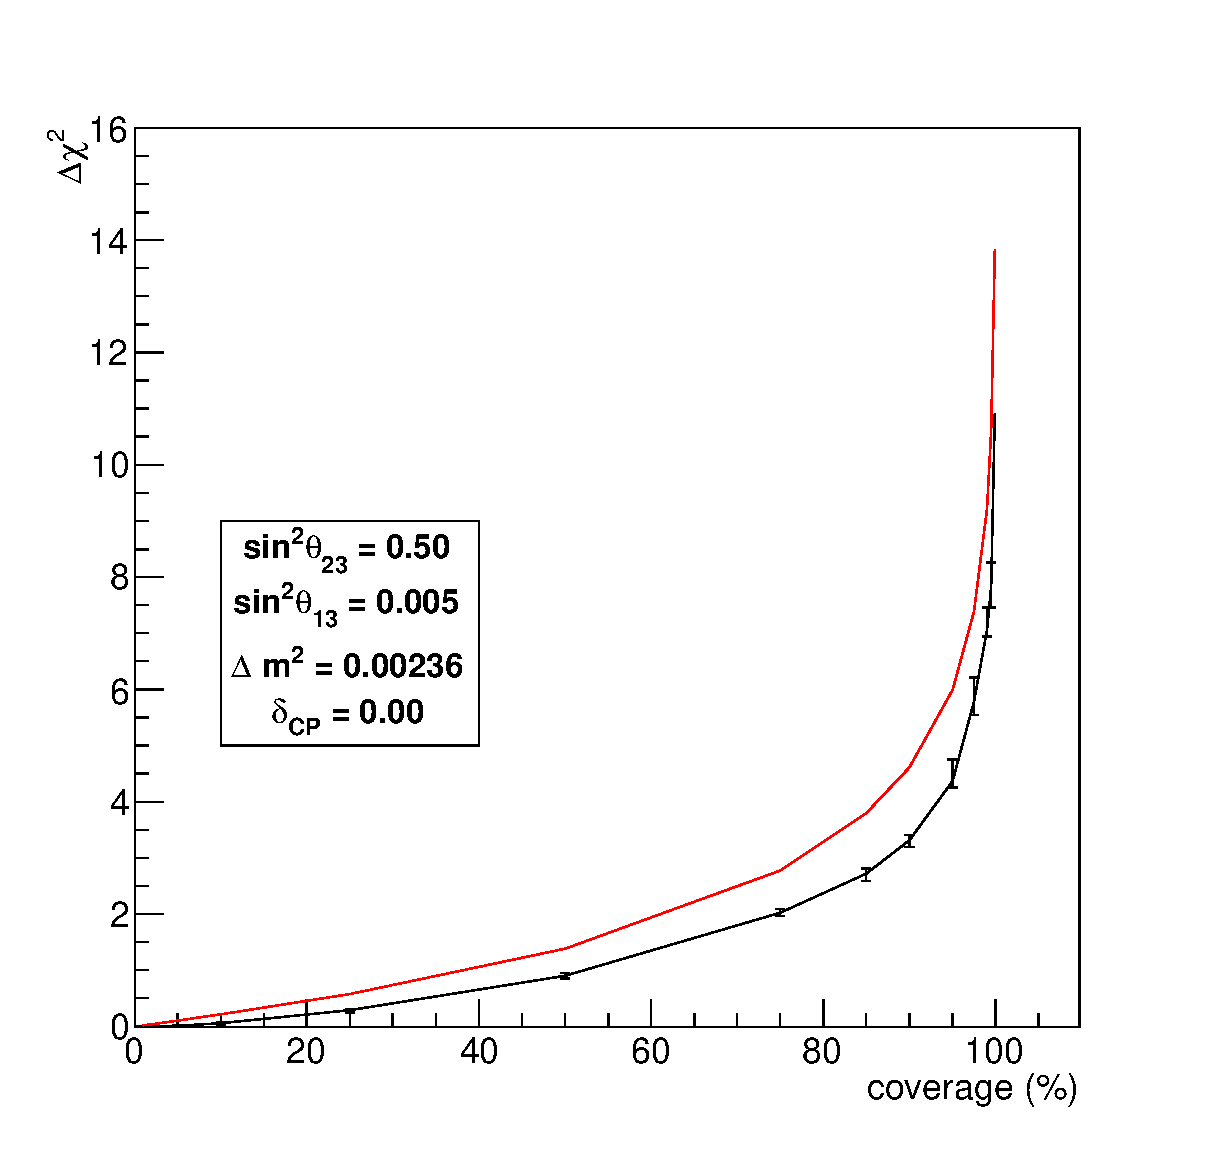
\includegraphics[width=14pc]{./images/appendix/coverage/coverage_study_2D_theta13_theta23_16.eps}
\center
\caption {
  Distribution of $\Delta\chi^{2}$ vs coverage in the ($sin^{2}\theta_{13}$,$sin^{2}\theta_{23}$) parameter space
  from 1k toy MC experiments generated with the Run 1+2+3 POT
  with statistical fluctuations at the oscillation point indicated in the legend. 
}
\label{fig:cov_2D_theta13_theta23_16}
\end{minipage}
\hspace{0.03\linewidth}
\begin{minipage}[t]{0.46\linewidth}
\center
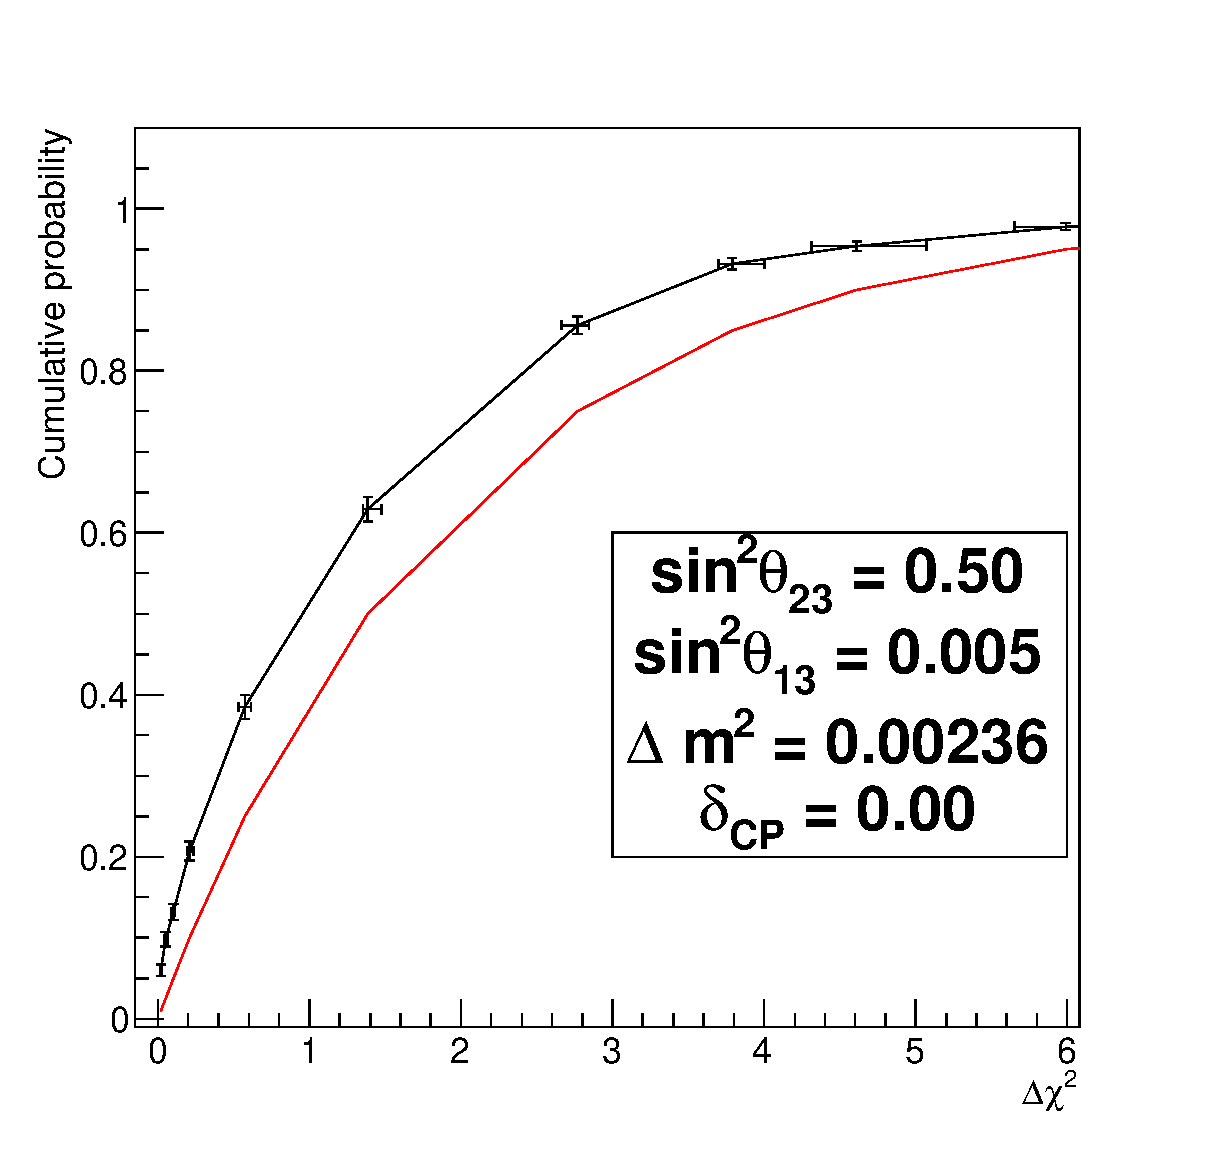
\includegraphics[width=14pc]{./images/appendix/coverage/coverage_study_2D_theta13_theta23_stats_new_16.eps}
\center
\caption {
  Distribution of cumulative probability vs $\Delta\chi^{2}$ in the ($sin^{2}\theta_{13}$,$sin^{2}\theta_{23}$) parameter space
  from 1k toy MC experiments generated with the Run 1+2+3 POT
  with statistical fluctuations at the oscillation point indicated in the legend. 
}
\label{fig:prob_2D_theta13_theta23_16}
\end{minipage}
\vfill
\vspace*{0.7cm}
\begin{minipage}[t]{0.46\linewidth}
\center
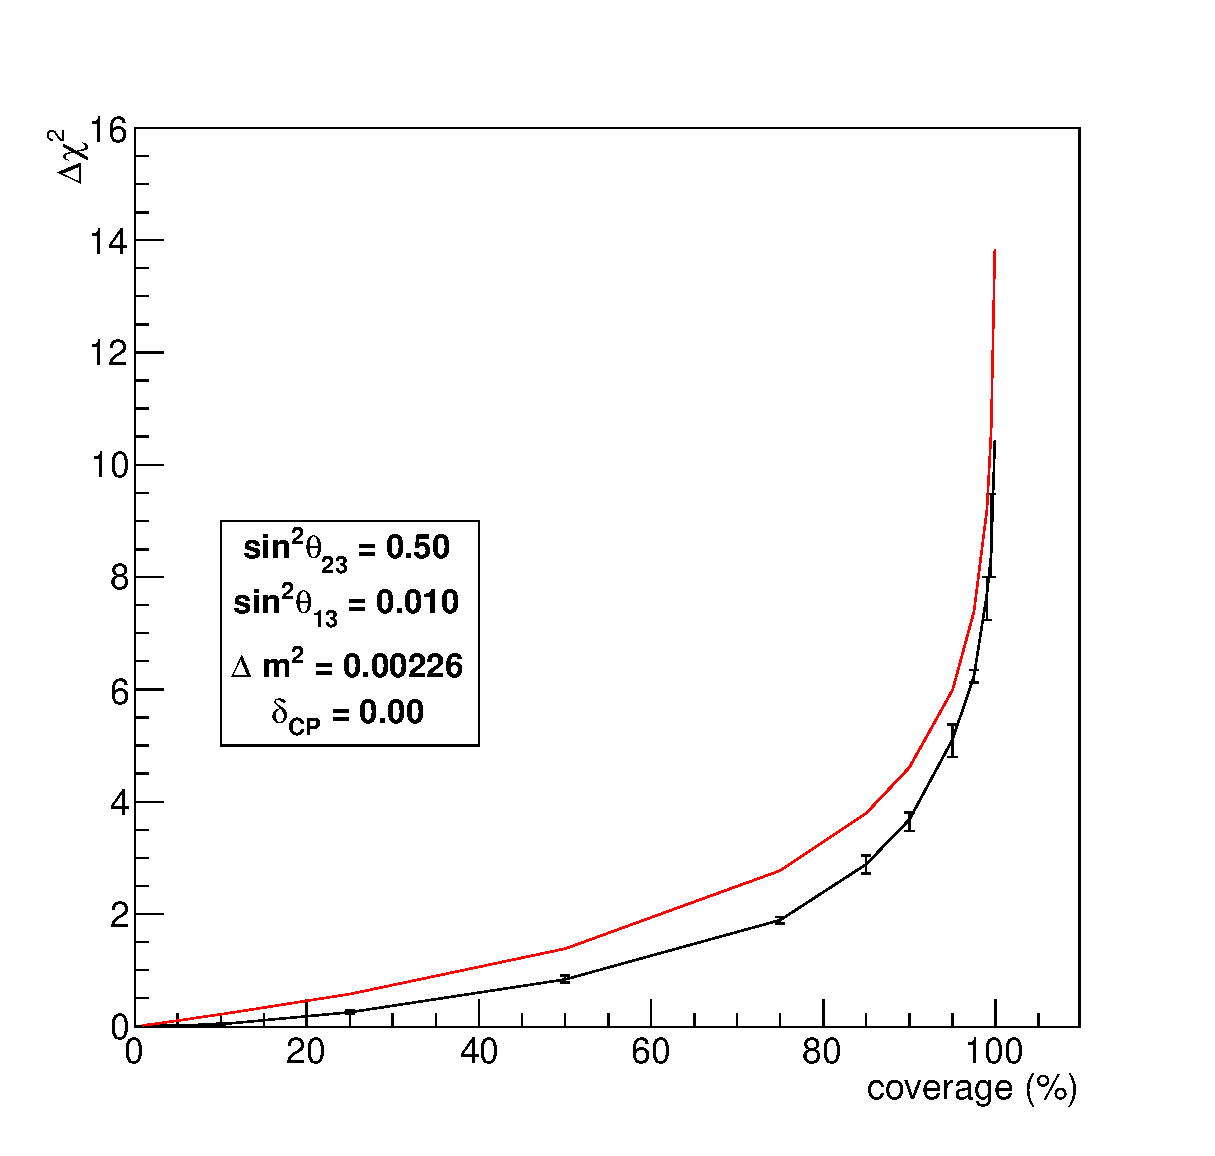
\includegraphics[width=14pc]{./images/appendix/coverage/coverage_study_2D_theta13_theta23_17.eps}
\center
\caption {
  Distribution of $\Delta\chi^{2}$ vs coverage in the ($sin^{2}\theta_{13}$,$sin^{2}\theta_{23}$) parameter space
  from 1k toy MC experiments generated with the Run 1+2+3 POT
  with statistical fluctuations at the oscillation point indicated in the legend. 
}
\label{fig:cov_2D_theta13_theta23_17}
\end{minipage}
\hspace{0.03\linewidth}
\begin{minipage}[t]{0.46\linewidth}
\center
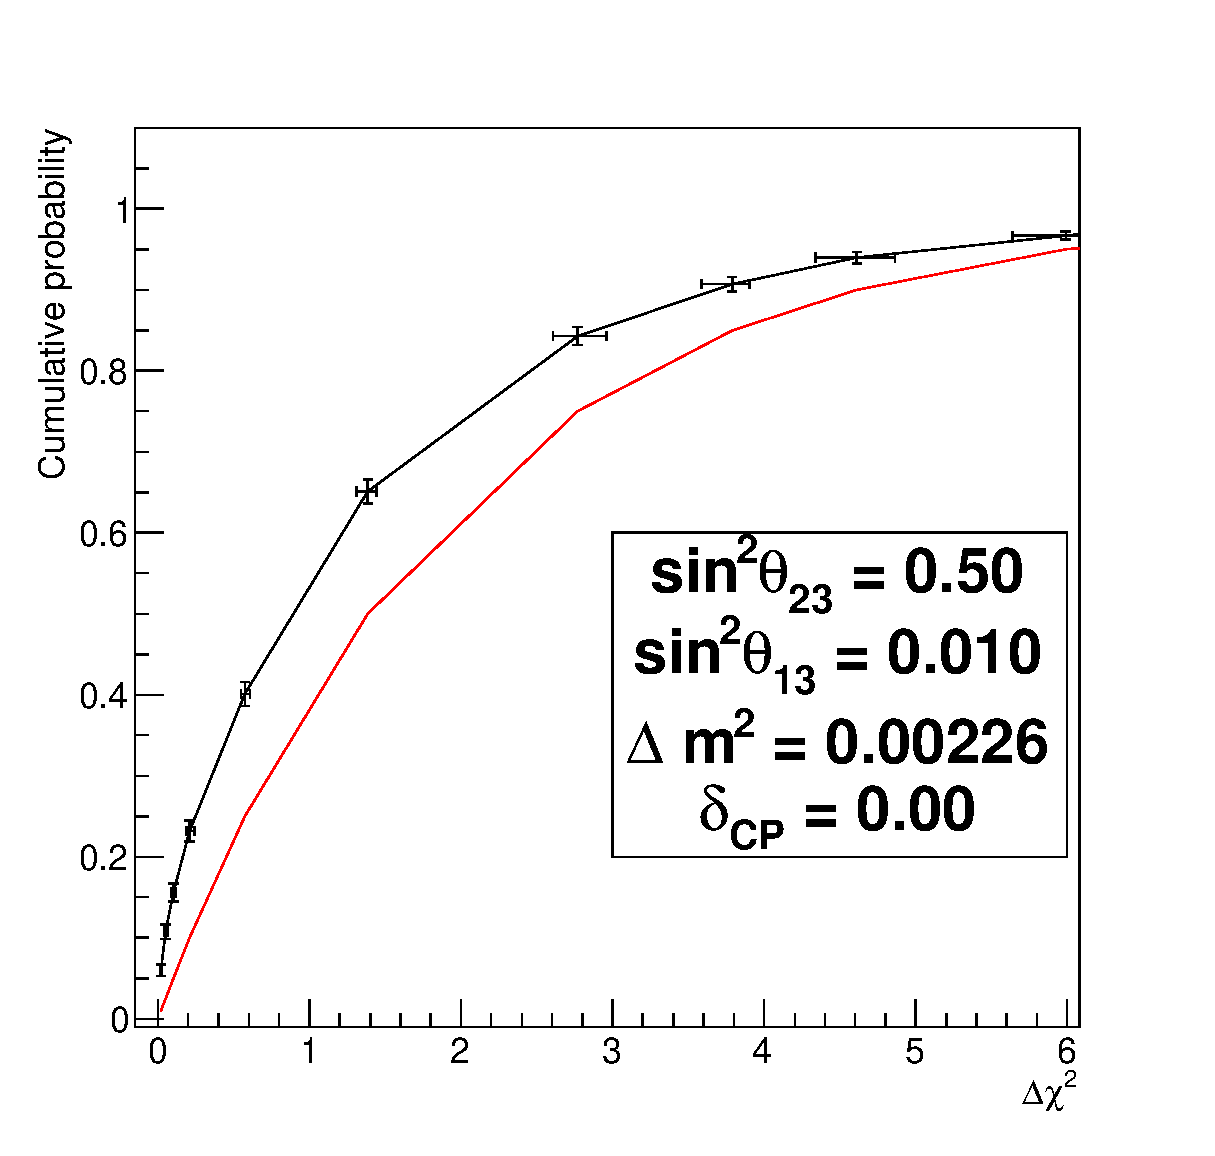
\includegraphics[width=14pc]{./images/appendix/coverage/coverage_study_2D_theta13_theta23_stats_new_17.eps}
\center
\caption {
  Distribution of cumulative probability vs $\Delta\chi^{2}$ in the ($sin^{2}\theta_{13}$,$sin^{2}\theta_{23}$) parameter space
  from 1k toy MC experiments generated with the Run 1+2+3 POT
  with statistical fluctuations at the oscillation point indicated in the legend. 
}
\label{fig:prob_2D_theta13_theta23_17}
\end{minipage}
\end{figure*}
\end{center}



\begin{center}
\begin{figure*}[htb]
\begin{minipage}[t]{0.46\linewidth}
\center
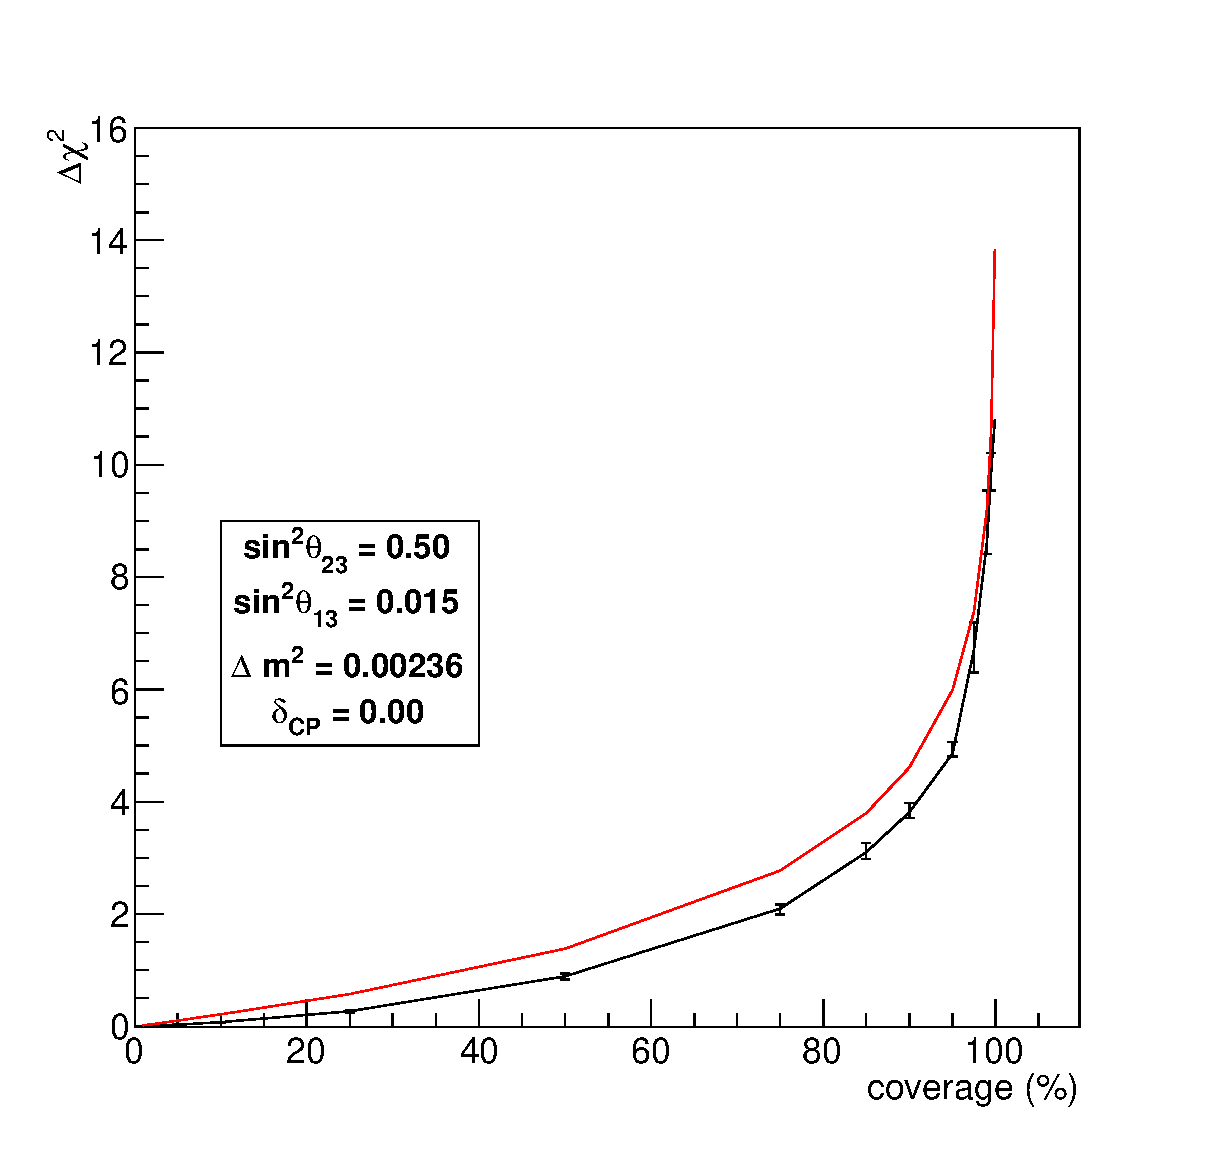
\includegraphics[width=14pc]{./images/appendix/coverage/coverage_study_2D_theta13_theta23_18.eps}
\center
\caption {
  Distribution of $\Delta\chi^{2}$ vs coverage in the ($sin^{2}\theta_{13}$,$sin^{2}\theta_{23}$) parameter space
  from 1k toy MC experiments generated with the Run 1+2+3 POT
  with statistical fluctuations at the oscillation point indicated in the legend. 
}
\label{fig:cov_2D_theta13_theta23_18}
\end{minipage}
\hspace{0.03\linewidth}
\begin{minipage}[t]{0.46\linewidth}
\center
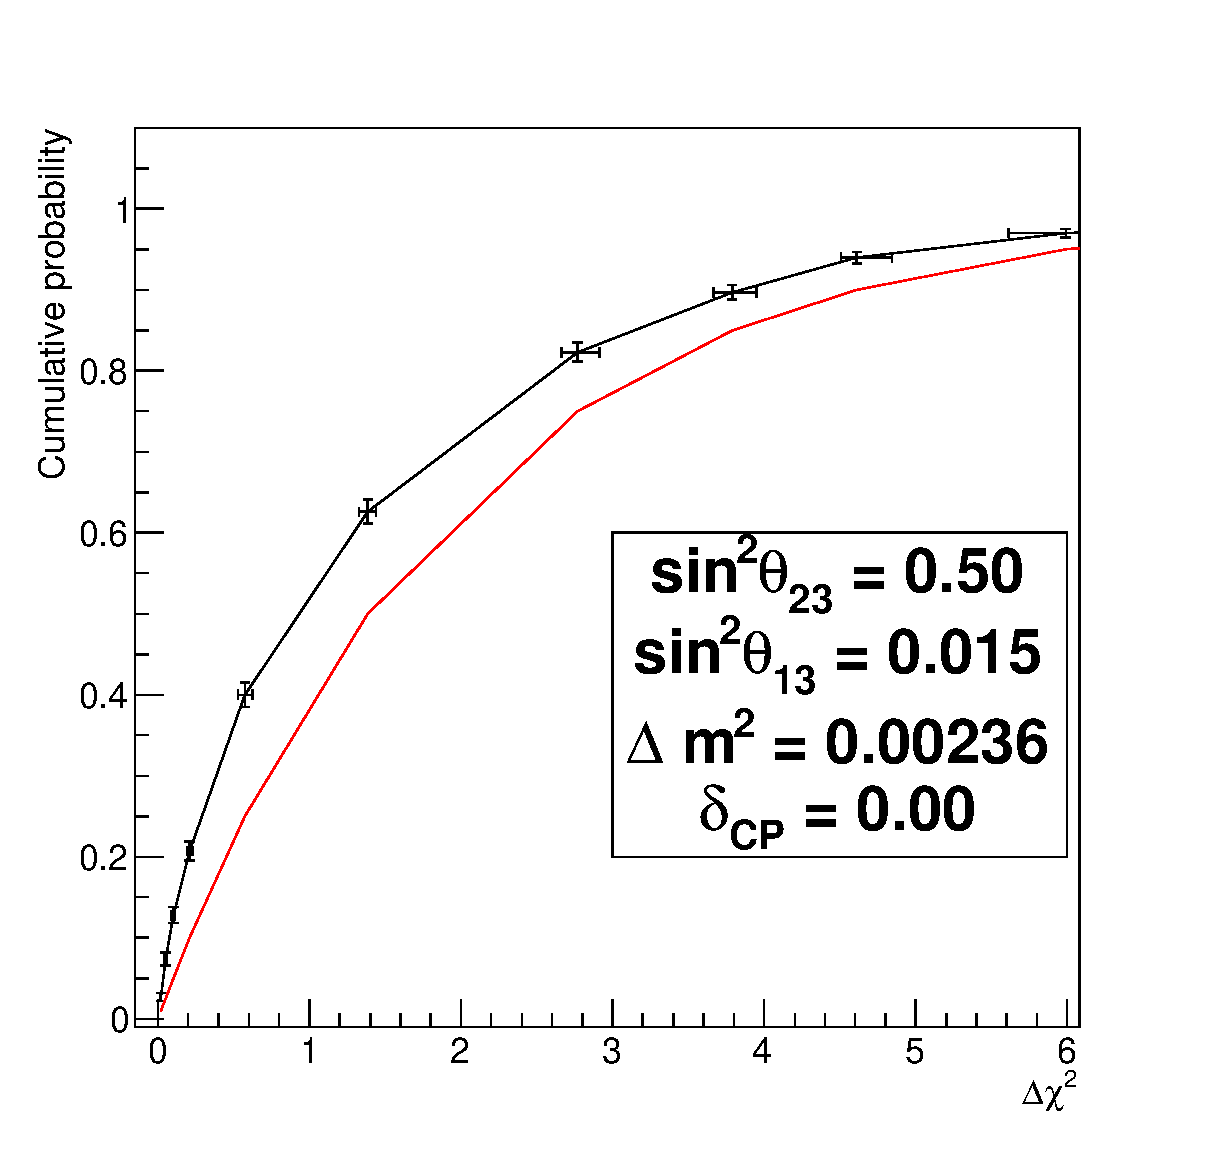
\includegraphics[width=14pc]{./images/appendix/coverage/coverage_study_2D_theta13_theta23_stats_new_18.eps}
\center
\caption {
  Distribution of cumulative probability vs $\Delta\chi^{2}$ in the ($sin^{2}\theta_{13}$,$sin^{2}\theta_{23}$) parameter space
  from 1k toy MC experiments generated with the Run 1+2+3 POT
  with statistical fluctuations at the oscillation point indicated in the legend. 
}
\label{fig:prob_2D_theta13_theta23_18}
\end{minipage}
\vfill
\vspace*{0.7cm}
\begin{minipage}[t]{0.46\linewidth}
\center
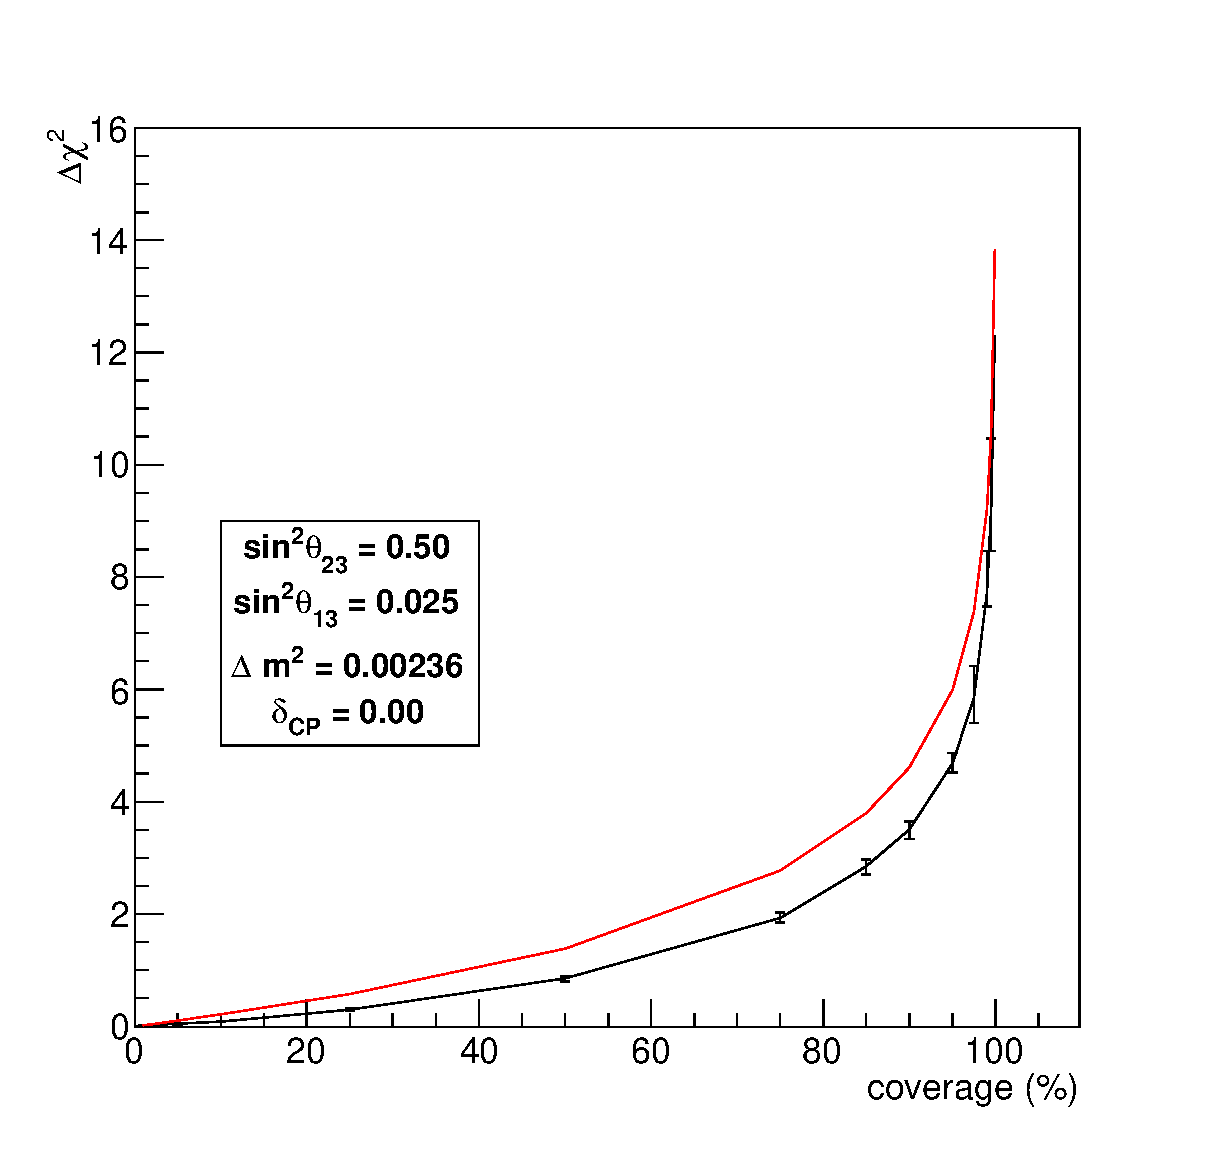
\includegraphics[width=14pc]{./images/appendix/coverage/coverage_study_2D_theta13_theta23_19.eps}
\center
\caption {
  Distribution of $\Delta\chi^{2}$ vs coverage in the ($sin^{2}\theta_{13}$,$sin^{2}\theta_{23}$) parameter space
  from 1k toy MC experiments generated with the Run 1+2+3 POT
  with statistical fluctuations at the oscillation point indicated in the legend. 
}
\label{fig:cov_2D_theta13_theta23_19}
\end{minipage}
\hspace{0.03\linewidth}
\begin{minipage}[t]{0.46\linewidth}
\center
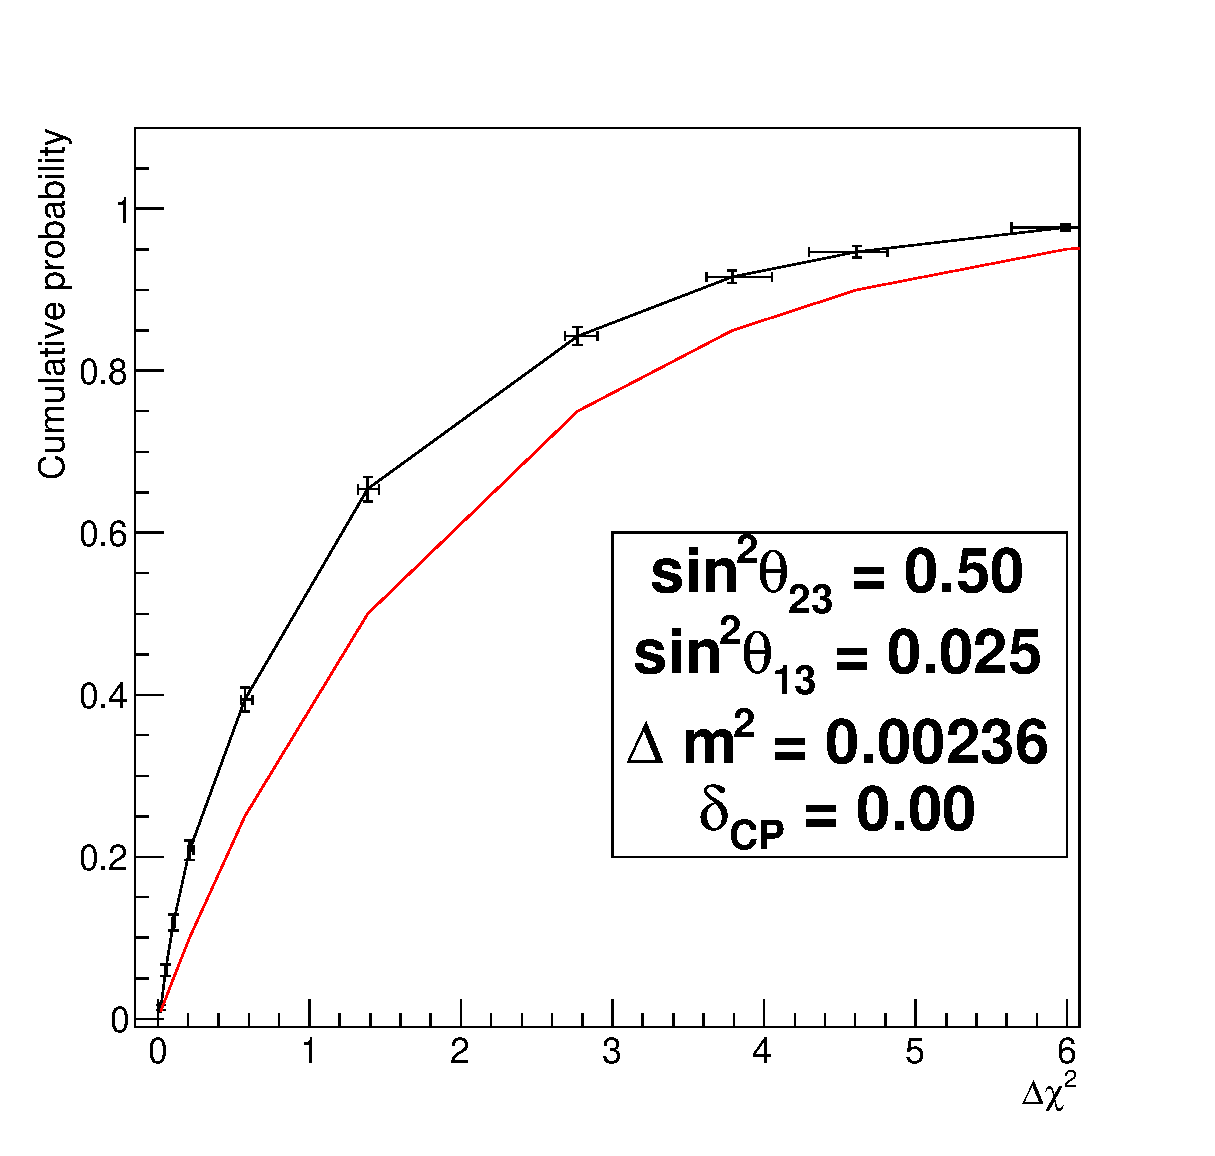
\includegraphics[width=14pc]{./images/appendix/coverage/coverage_study_2D_theta13_theta23_stats_new_19.eps}
\center
\caption {
  Distribution of cumulative probability vs $\Delta\chi^{2}$ in the ($sin^{2}\theta_{13}$,$sin^{2}\theta_{23}$) parameter space
  from 1k toy MC experiments generated with the Run 1+2+3 POT
  with statistical fluctuations at the oscillation point indicated in the legend. 
}
\label{fig:prob_2D_theta13_theta23_19}
\end{minipage}
\end{figure*}
\end{center}


\begin{center}
\begin{figure*}[htb]
\begin{minipage}[t]{0.46\linewidth}
\center
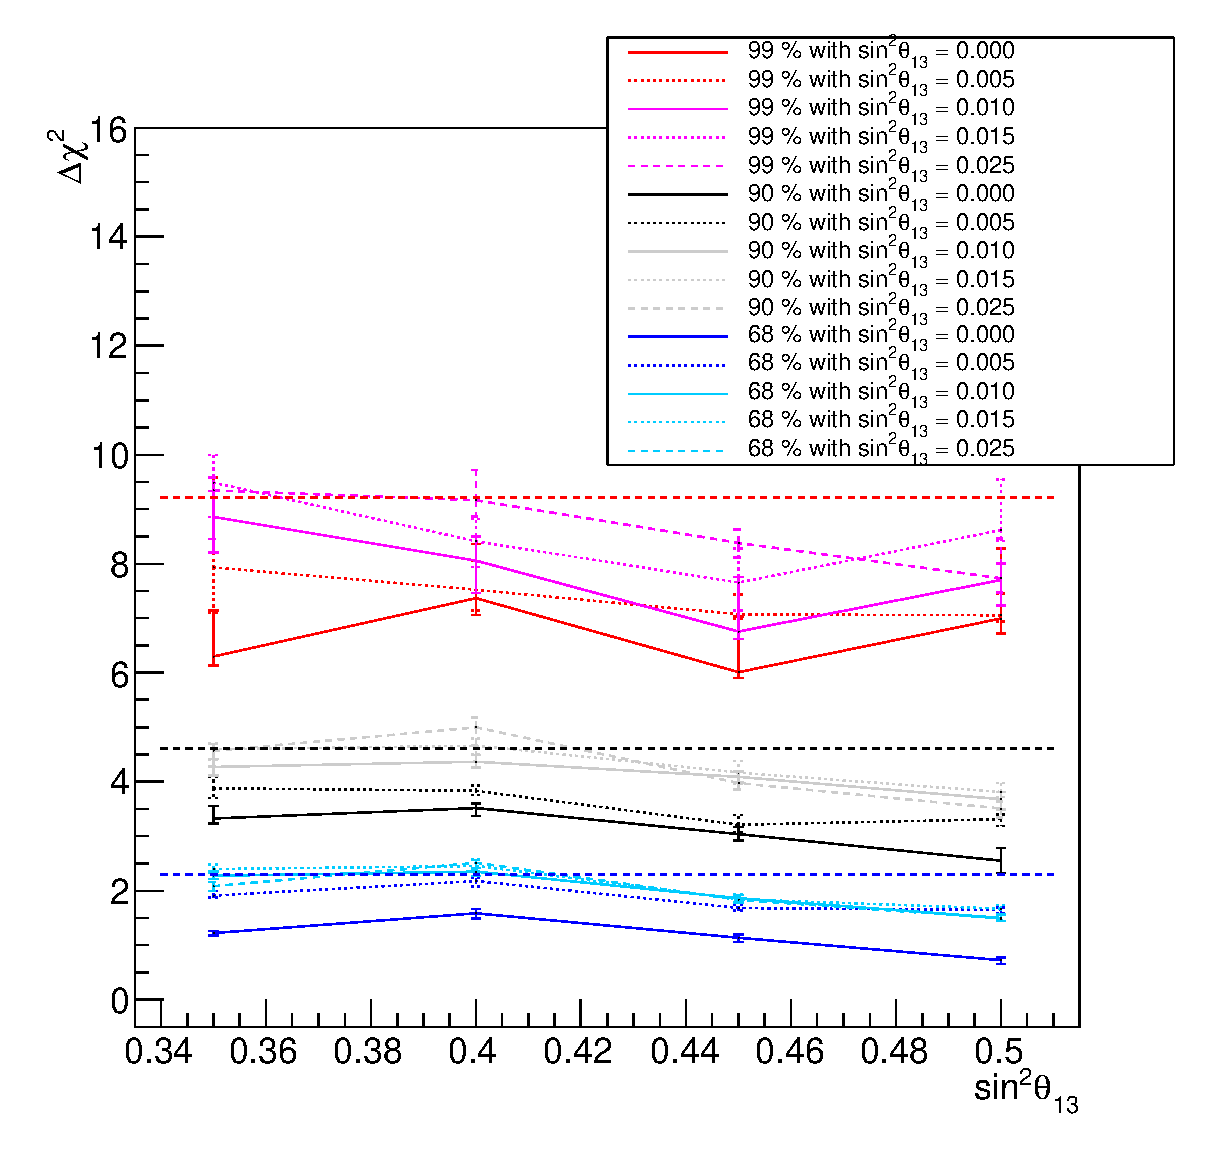
\includegraphics[width=14pc]{./images/appendix/coverage/coverage_study_2D_theta13_theta23_all_1.eps}
\center
\caption {
    Summary of figures \ref{fig:cov_2D_theta13_theta23_0}-\ref{fig:cov_2D_theta13_theta23_19}
showing the value of $\Delta\chi^{2}$ at 99\%, 90\% and 68\% confidence intervals vs the value of $sin^{2}\theta_{23}$.
Horizontal dashed lines show the canonical $\Delta\chi^{2}$ value for 2 degrees of freedom.
	}
\label{fig:cov_2D_theta13_theta23_all_1}
\end{minipage}
\hspace{0.03\linewidth}
\begin{minipage}[t]{0.46\linewidth}
\center
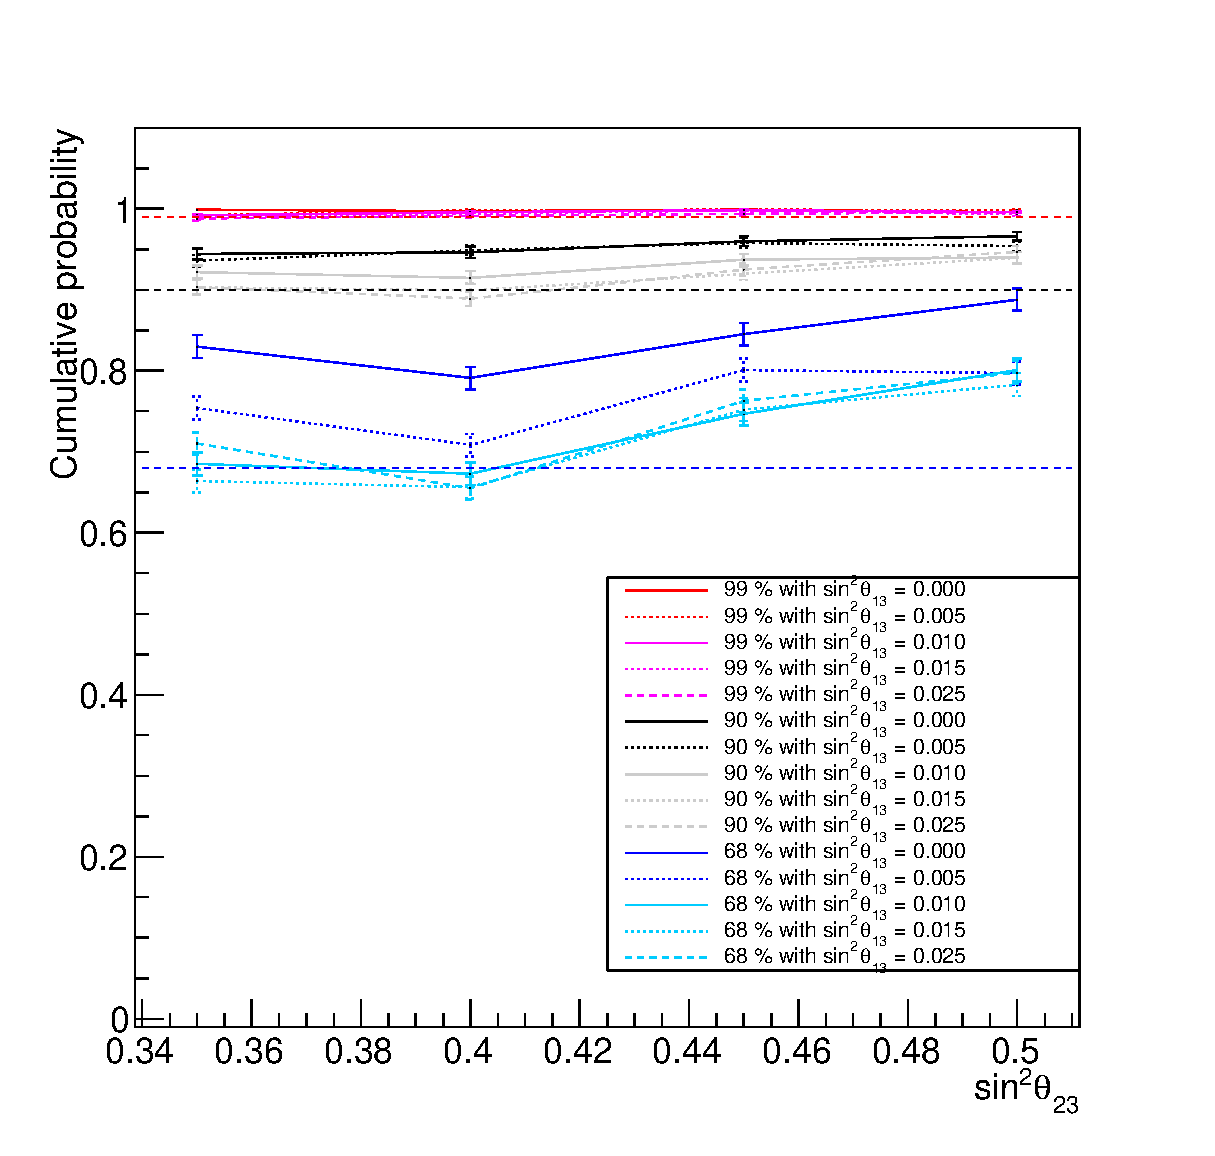
\includegraphics[width=14pc]{./images/appendix/coverage/coverage_study_2D_theta13_theta23_stats_new_all_2.eps}
\center
\caption {
    Summary of figures \ref{fig:prob_2D_theta13_theta23_0}-\ref{fig:prob_2D_theta13_theta23_19}
showing the value of cumulative probability for $\Delta\chi^{2}=9.21$ (canonical value for 99\%), $\Delta\chi^{2}=4.61$ (canonical value for 90\%) and $\Delta\chi^{2}=2.30$ (canonical value for 68\%) vs the value of $sin^{2}\theta_{23}$.
	}
\label{fig:prob_2D_theta13_theta23_all_1}
\end{minipage}
\vfill
\vspace*{0.7cm}
\begin{minipage}[t]{0.46\linewidth}
\center
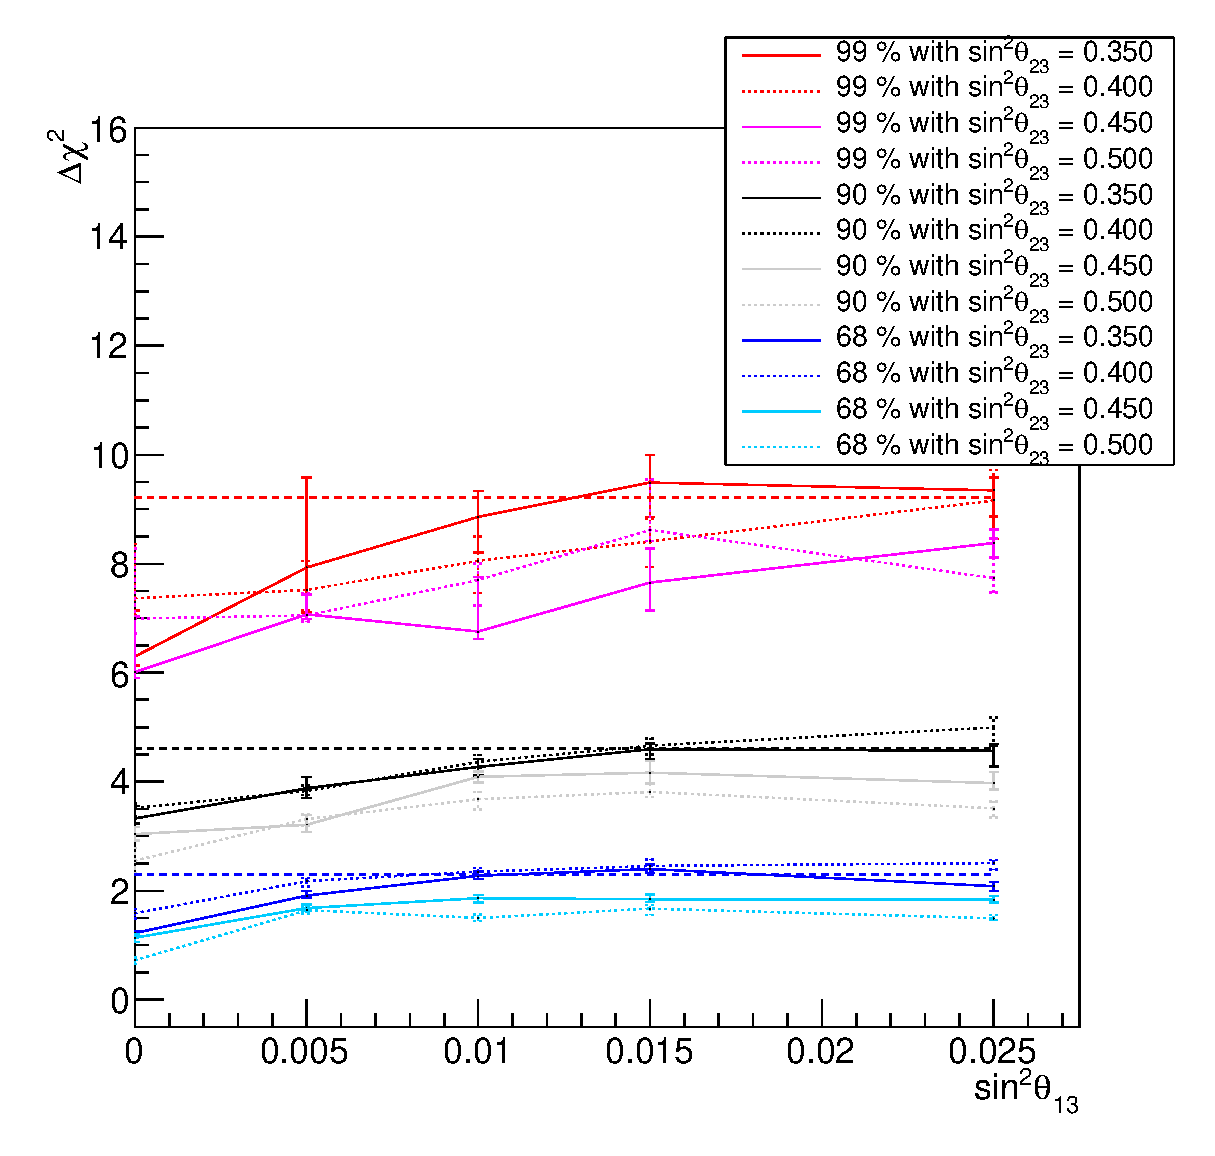
\includegraphics[width=14pc]{./images/appendix/coverage/coverage_study_2D_theta13_theta23_all_2.eps}
\center
\caption {
    Summary of figures \ref{fig:cov_2D_theta13_theta23_0}-\ref{fig:cov_2D_theta13_theta23_19}
showing the value of $\Delta\chi^{2}$ at 99\%, 90\% and 68\% confidence intervals vs the value of $sin^{2}\theta_{13}$.
Horizontal dashed lines show the canonical $\Delta\chi^{2}$ value for 2 degrees of freedom.
	}
\label{fig:cov_2D_theta13_theta23_all_2}
\end{minipage}
\hspace{0.03\linewidth}
\begin{minipage}[t]{0.46\linewidth}
\center
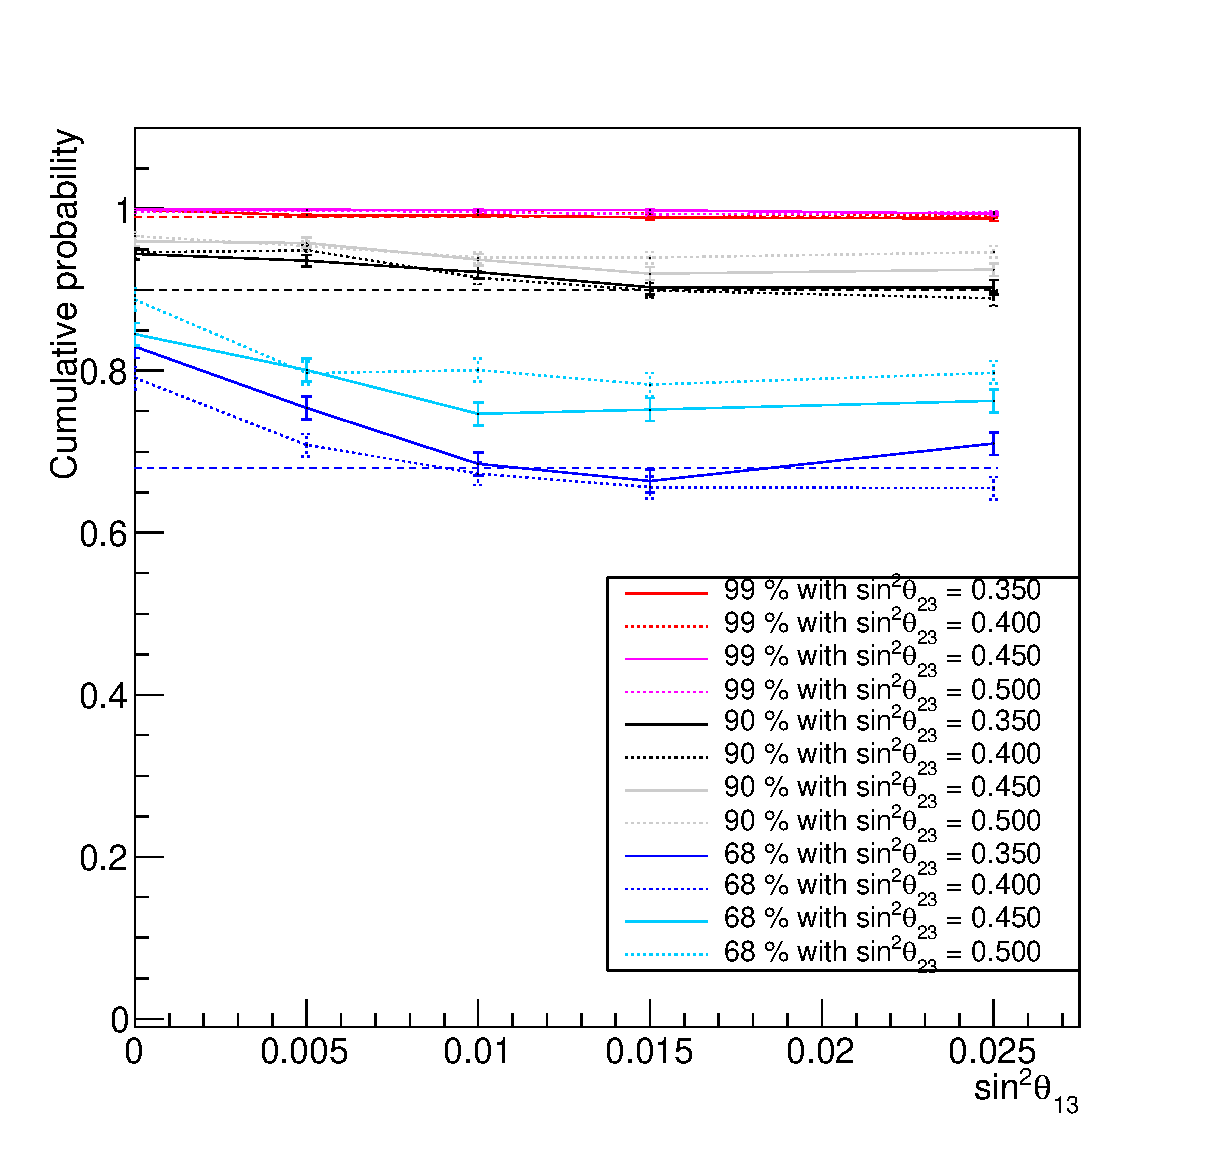
\includegraphics[width=14pc]{./images/appendix/coverage/coverage_study_2D_theta13_theta23_stats_new_all_1.eps}
\center
\caption {
    Summary of figures \ref{fig:prob_2D_theta13_theta23_0}-\ref{fig:prob_2D_theta13_theta23_19}
showing the value of cumulative probability for $\Delta\chi^{2}=9.21$ (canonical value for 99\%), $\Delta\chi^{2}=4.61$ (canonical value for 90\%) and $\Delta\chi^{2}=2.30$ (canonical value for 68\%) vs the value of $sin^{2}\theta_{13}$.
	}
\label{fig:prob_2D_theta13_theta23_all_2}
\end{minipage}
\end{figure*}
\end{center}


\begin{center}
\begin{figure*}[htb]
\begin{minipage}[t]{0.46\linewidth}
\center
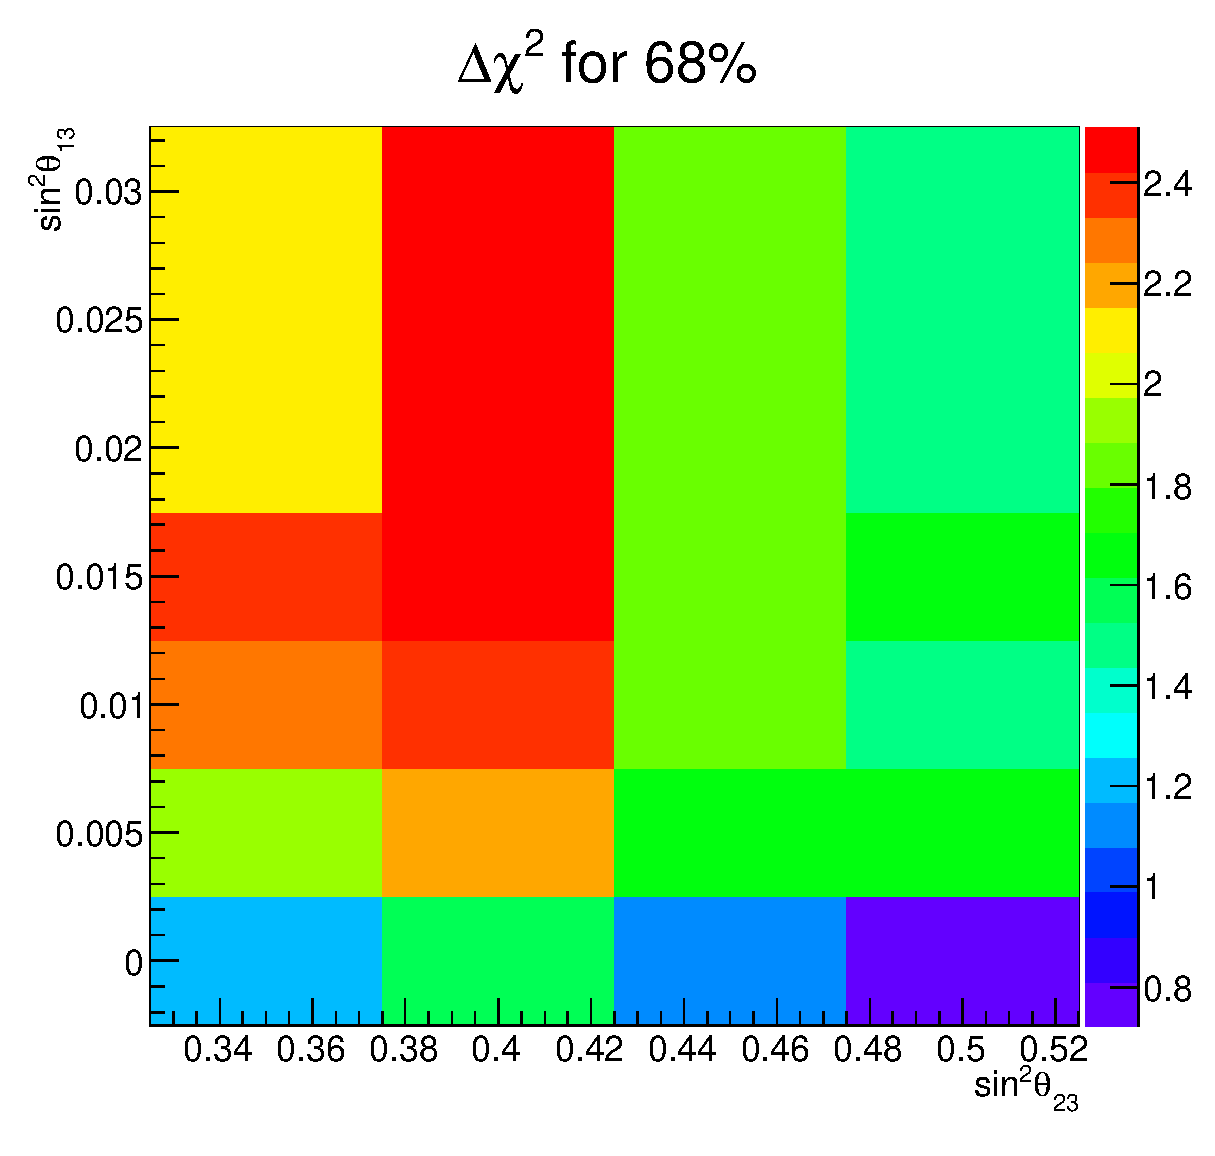
\includegraphics[width=14pc]{./images/appendix/coverage/coverage_study_2D_theta13_theta23_68.eps}
\center
\caption {
    Summary of figures \ref{fig:cov_2D_theta13_theta23_0}-\ref{fig:cov_2D_theta13_theta23_19}
showing the value of $\Delta\chi^{2}$ at 68\% confidence intervals in Z axis (color) vs the value of $sin^{2}\theta_{23}$ in X axis and $sin^{2}\theta_{13}$ in Y axis.
	}
\label{fig:cov_2D_theta13_theta23_68}
\end{minipage}
\hspace{0.03\linewidth}
\begin{minipage}[t]{0.46\linewidth}
\center
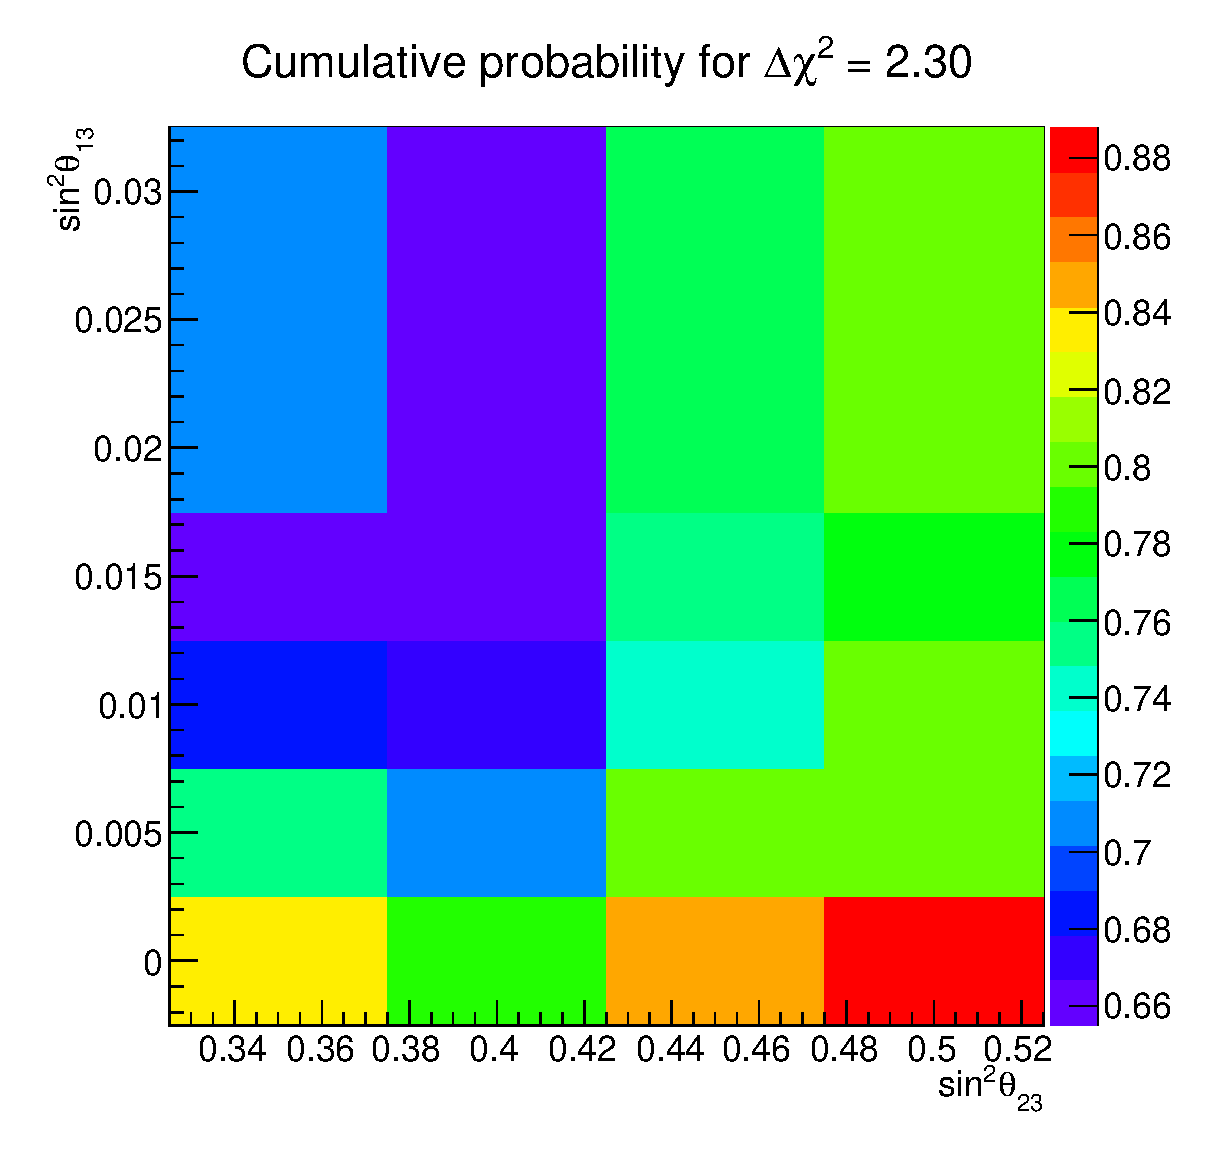
\includegraphics[width=14pc]{./images/appendix/coverage/coverage_study_2D_theta13_theta23_stats_new_68.eps}
\caption {
    Summary of figures \ref{fig:prob_2D_theta13_theta23_0}-\ref{fig:prob_2D_theta13_theta23_19}
showing the value of the cumulative probability for $\Delta\chi^{2} = 2.30$ in Z axis (color) vs the value of $sin^{2}\theta_{23}$ in X axis and $sin^{2}\theta_{13}$ in Y axis.
	}
\label{fig:prob_2D_theta13_theta23_68}
\end{minipage}
\vfill
\vspace*{0.7cm}
\begin{minipage}[t]{0.46\linewidth}
\center
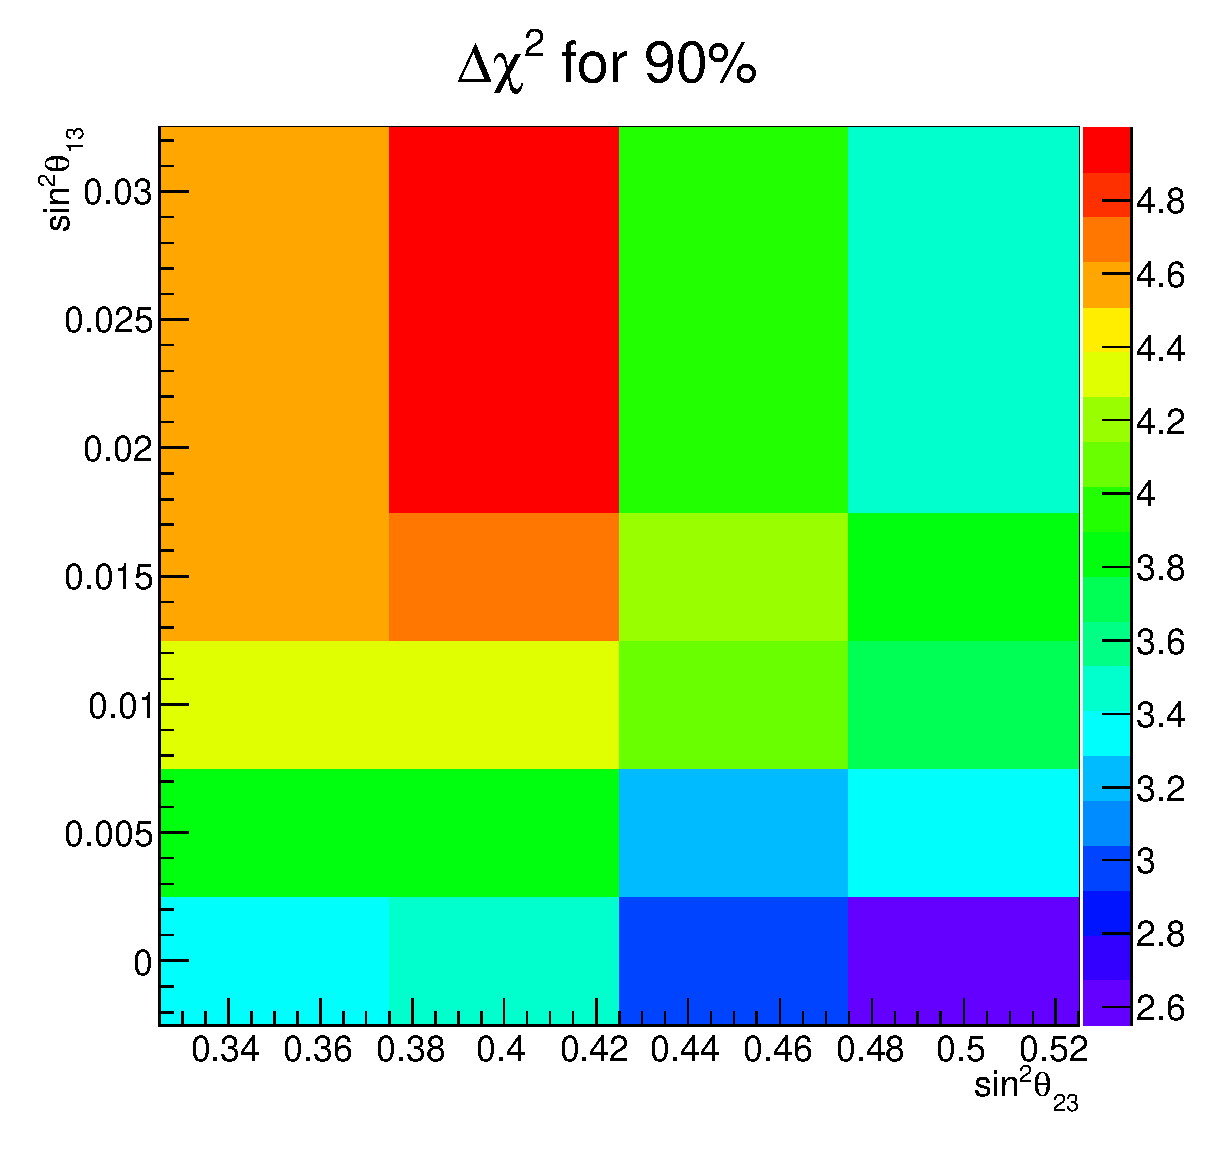
\includegraphics[width=14pc]{./images/appendix/coverage/coverage_study_2D_theta13_theta23_90.eps}
\caption {
    Summary of figures \ref{fig:cov_2D_theta13_theta23_0}-\ref{fig:cov_2D_theta13_theta23_19}
showing the value of $\Delta\chi^{2}$ at 90\% confidence intervals in Z axis (color) vs the value of $sin^{2}\theta_{23}$ in X axis and $sin^{2}\theta_{13}$ in Y axis.
		}
\label{fig:cov_2D_theta13_theta23_90}
\end{minipage}
\hspace{0.03\linewidth}
\begin{minipage}[t]{0.46\linewidth}
\center
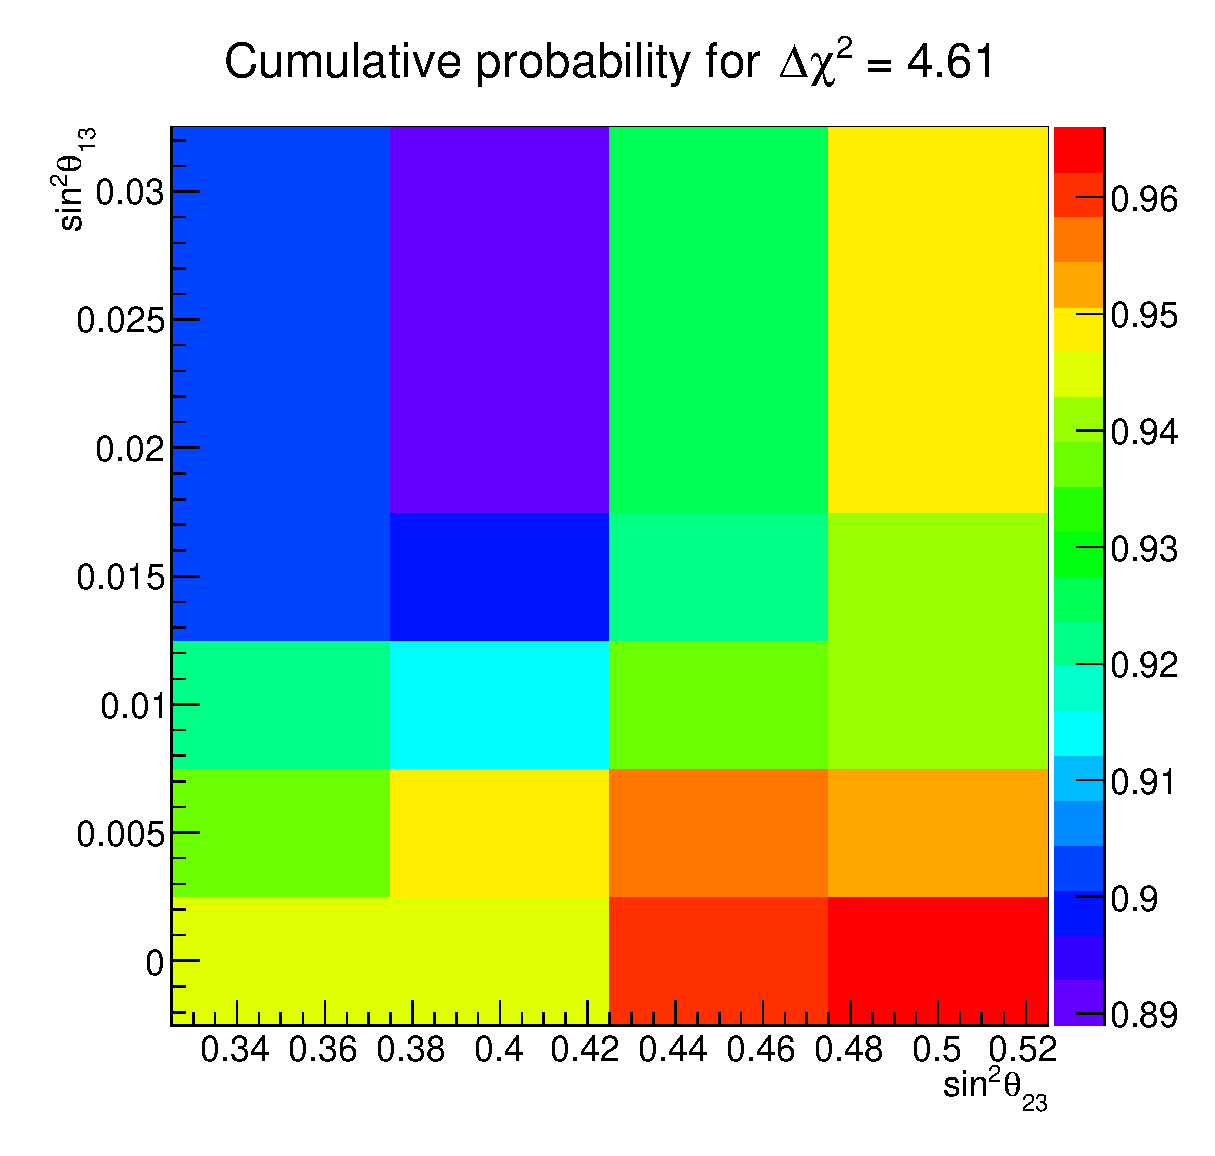
\includegraphics[width=14pc]{./images/appendix/coverage/coverage_study_2D_theta13_theta23_stats_new_90.eps}
\caption {
    Summary of figures \ref{fig:prob_2D_theta13_theta23_0}-\ref{fig:prob_2D_theta13_theta23_19}
showing the value of the cumulative probability for $\Delta\chi^{2} = 4.61$ in Z axis (color) vs the value of $sin^{2}\theta_{23}$ in X axis and $sin^{2}\theta_{13}$ in Y axis.
	}
\label{fig:prob_2D_theta13_theta23_90}
\end{minipage}
\vfill
\vspace*{0.7cm}
\center
\begin{minipage}[t]{0.46\linewidth}
\center
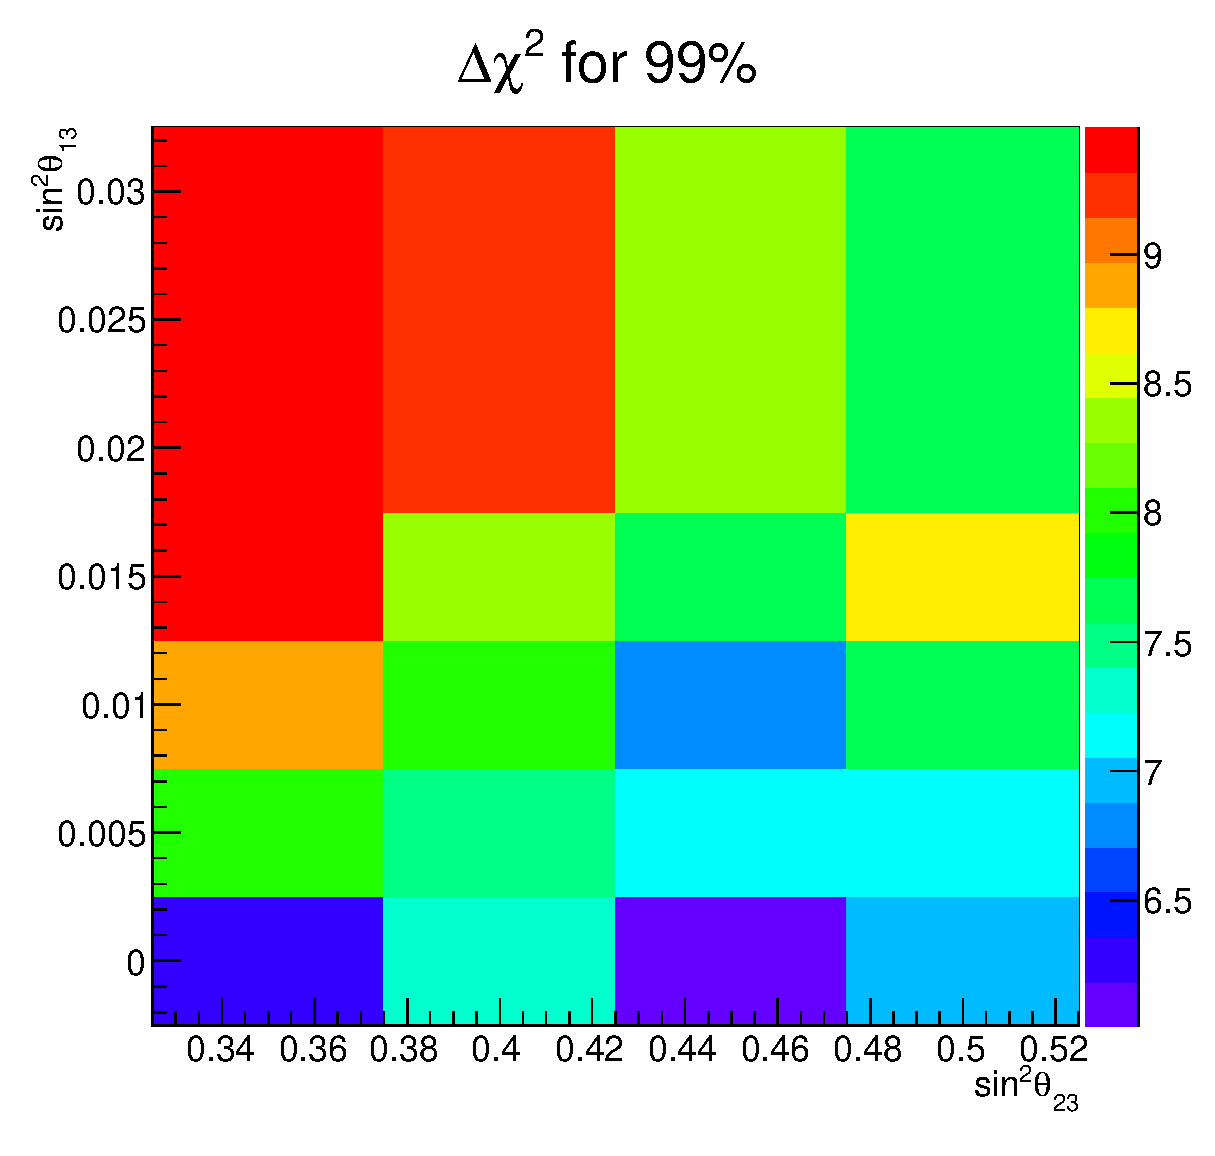
\includegraphics[width=14pc]{./images/appendix/coverage/coverage_study_2D_theta13_theta23_99.eps}
\caption {
    Summary of figures \ref{fig:cov_2D_theta13_theta23_0}-\ref{fig:cov_2D_theta13_theta23_19}
showing the value of $\Delta\chi^{2}$ at 99\% confidence intervals in Z axis (color) vs the value of $sin^{2}\theta_{23}$ in X axis and $sin^{2}\theta_{13}$ in Y axis.
	}
\label{fig:cov_2D_theta13_theta23_99}
\end{minipage}
\hspace{0.03\linewidth}
\begin{minipage}[t]{0.46\linewidth}
\center
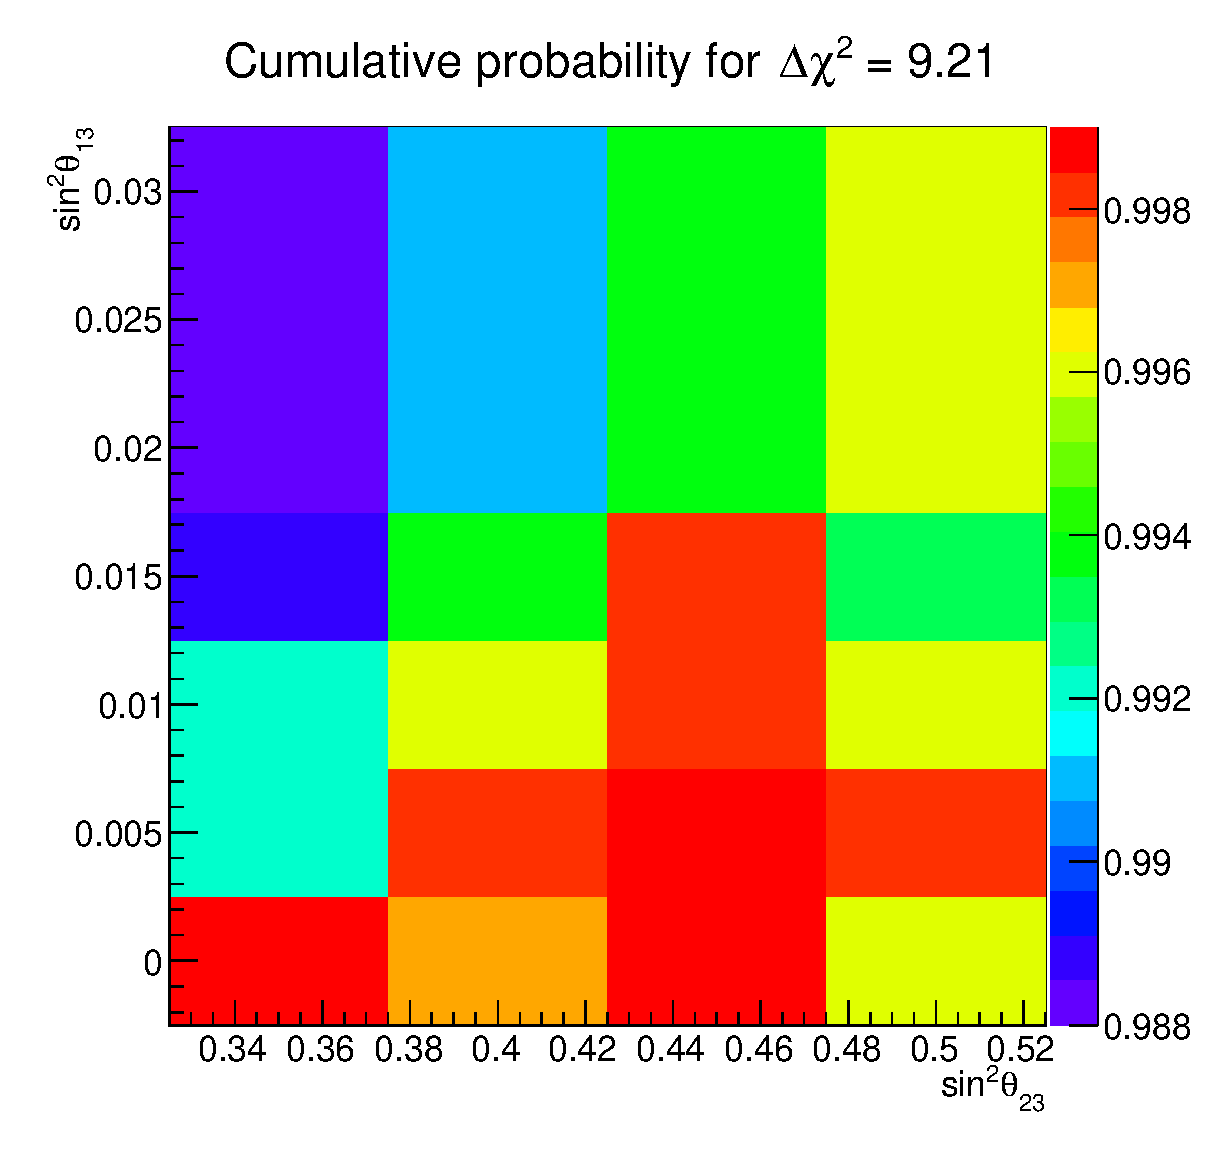
\includegraphics[width=14pc]{./images/appendix/coverage/coverage_study_2D_theta13_theta23_stats_new_99.eps}
\caption {
    Summary of figures \ref{fig:prob_2D_theta13_theta23_0}-\ref{fig:prob_2D_theta13_theta23_19}
showing the value of the cumulative probability for $\Delta\chi^{2} = 9.21$ in Z axis (color) vs the value of $sin^{2}\theta_{23}$ in X axis and $sin^{2}\theta_{13}$ in Y axis.
	}
\label{fig:prob_2D_theta13_theta23_99}
\end{minipage}
\end{figure*}
\end{center}

\clearpage
\subsection{Coverage studies in 2D including systematic variations}
\label{app:cov:syst}

The coverage studies in this subsection are presented
for the same oscillation points in the 2D parameter spaces seen previously, now applying 
systematic variations to the toy MC experiments and fitting for systematics along with the
corresponding oscillation parameters. The procedure is the following:

\begin{itemize}
\item{At a certain oscillation point, 1k toy experiments were created with statistical fluctuations and random systematic variations.}
\item{A first value of $\chi^{2}$ ($\chi^{2} _{init}$) was obtained for each toy experiment fixing the oscillation parameters to the true input values and fitting the systematic parameters.}
\item{A second fit was performed for each toy experiment fitting oscillation parameters and systematic errors, obtaining $\chi^{2} _{bf}$. Like in the case with only statistical fluctuations, the oscillation parameters included in the fit were the ones corresponding to the parameter space under study.}
\item{The value of $\Delta\chi^{2}$ was calculated for each toy experiment as the difference  $\Delta\chi^{2} = \chi^{2}_{init} - \chi^{2}_{bf}$, and the plots explained for the tests with statistical fluctuations only were made.}
\end{itemize}

In this subsection only summary plots like Fig. \ref{fig:cov_2D_theta23_dmsq_all} and \ref{fig:prob_2D_theta23_dmsq_all} in previous subsection are presented. They are built in the same way, first plotting the distribution of $\Delta\chi^{2}$ vs coverage like in Figs. \ref{fig:cov_2D_theta23_dmsq_0}-\ref{fig:cov_2D_theta23_dmsq_3}, and also the cumulative probability vs $\Delta\chi^{2}$ like in Figs. \ref{fig:prob_2D_theta23_dmsq_0}-\ref{fig:prob_2D_theta23_dmsq_3}, but those plots were omitted now. 
Thus, Figs.\ref{fig:cov_2D_theta23_dmsq_syst_all} and \ref{fig:prob_2D_theta23_dmsq_syst_all} are the summary plots for the 2D parameter space ($sin^{2}\theta_{23}$,$|\Delta m^{2}|$), Figs. \ref{fig:cov_2D_theta13_dmsq_syst_all} and \ref{fig:prob_2D_theta13_dmsq_syst_all}  for the 2D parameter space ($sin^{2}\theta_{13}$,$|\Delta m^{2}|$) and Figs.  \ref{fig:cov_2D_theta13_deltacp_syst_all} and \ref{fig:prob_2D_theta13_deltacp_syst_all} for the 2D parameter space ($sin^{2}\theta_{13}$,$\delta_{CP}$).

For the 2D parameter space ($sin^{2}\theta_{13}$,$sin^{2}\theta_{23}$) summaries are presented in Fig. \ref{fig:cov_2D_theta13_theta23_syst_all_1} and in Fig. \ref{fig:cov_2D_theta13_theta23_syst_all_2} showing the values of $\Delta\chi^{2}$ vs $sin^{2}\theta_{23}$ and $sin^{2}\theta_{13}$ respectively and then a summary is presented with the value of $\Delta\chi^{2}$ in Z axis (color) vs $sin^{2}\theta_{23}$ in X axis and $sin^{2}\theta_{13}$ in Y axis at 68\% confidence interval in Fig.\ref{fig:cov_2D_theta13_theta23_syst_68}, at 90\% confidence interval in Fig. \ref{fig:cov_2D_theta13_theta23_syst_90} and at 99\%  confidence interval in Fig. \ref{fig:cov_2D_theta13_theta23_syst_99}.
Similarly for cumulative probability in Fig. \ref{fig:prob_2D_theta13_theta23_syst_all_1}  etc. 

%Figures  \ref{fig:cov_2D_theta23_dmsq_syst_0}-\ref{fig:cov_2D_theta23_dmsq_syst_3} show the distribution of $\Delta\chi^{2}$ vs coverage
%in the 2D parameter space ($sin^{2}\theta_{23}$,$|\Delta m^{2}|$) for different oscillation points and a summary in Fig. \ref{fig:cov_2D_theta23_dmsq_syst_all}.
%Similarly for the 2D parameter space ($sin^{2}\theta_{13}$,$|\Delta m^{2}|$) in Figs. \ref{fig:cov_2D_theta13_dm23sq_syst_0}-\ref{fig:cov_2D_theta13_dm23sq_syst_all},
%and for the 2D parameter space ($sin^{2}\theta_{13}$,$\delta_{CP}$) in Figs. \ref{fig:cov_2D_theta13_deltacp_syst_0}-\ref{fig:cov_2D_theta13_deltacp_syst_all} where the
%canonical values for 1 and 2 degrees of freedom are both included. Finally the study in the parameter space ($sin^{2}\theta_{13}$,$sin^{2}\theta_{23}$)
%is presented in Figs. \ref{fig:cov_2D_theta13_theta23_syst_0}-\ref{fig:cov_2D_theta13_theta23_syst_19} and two summaries in
%Fig. \ref{fig:cov_2D_theta13_theta23_syst_all_1} and in Fig. \ref{fig:cov_2D_theta13_theta23_syst_all_2}. 

Results obtained in this section including systematic variations are similar to the ones with statistical fluctuations only. 

%% FIGURES FOR 2D theta23-DMsq
%\begin{center}
%\begin{figure*}[htb]
%\begin{minipage}[t]{0.46\linewidth}
%\center
%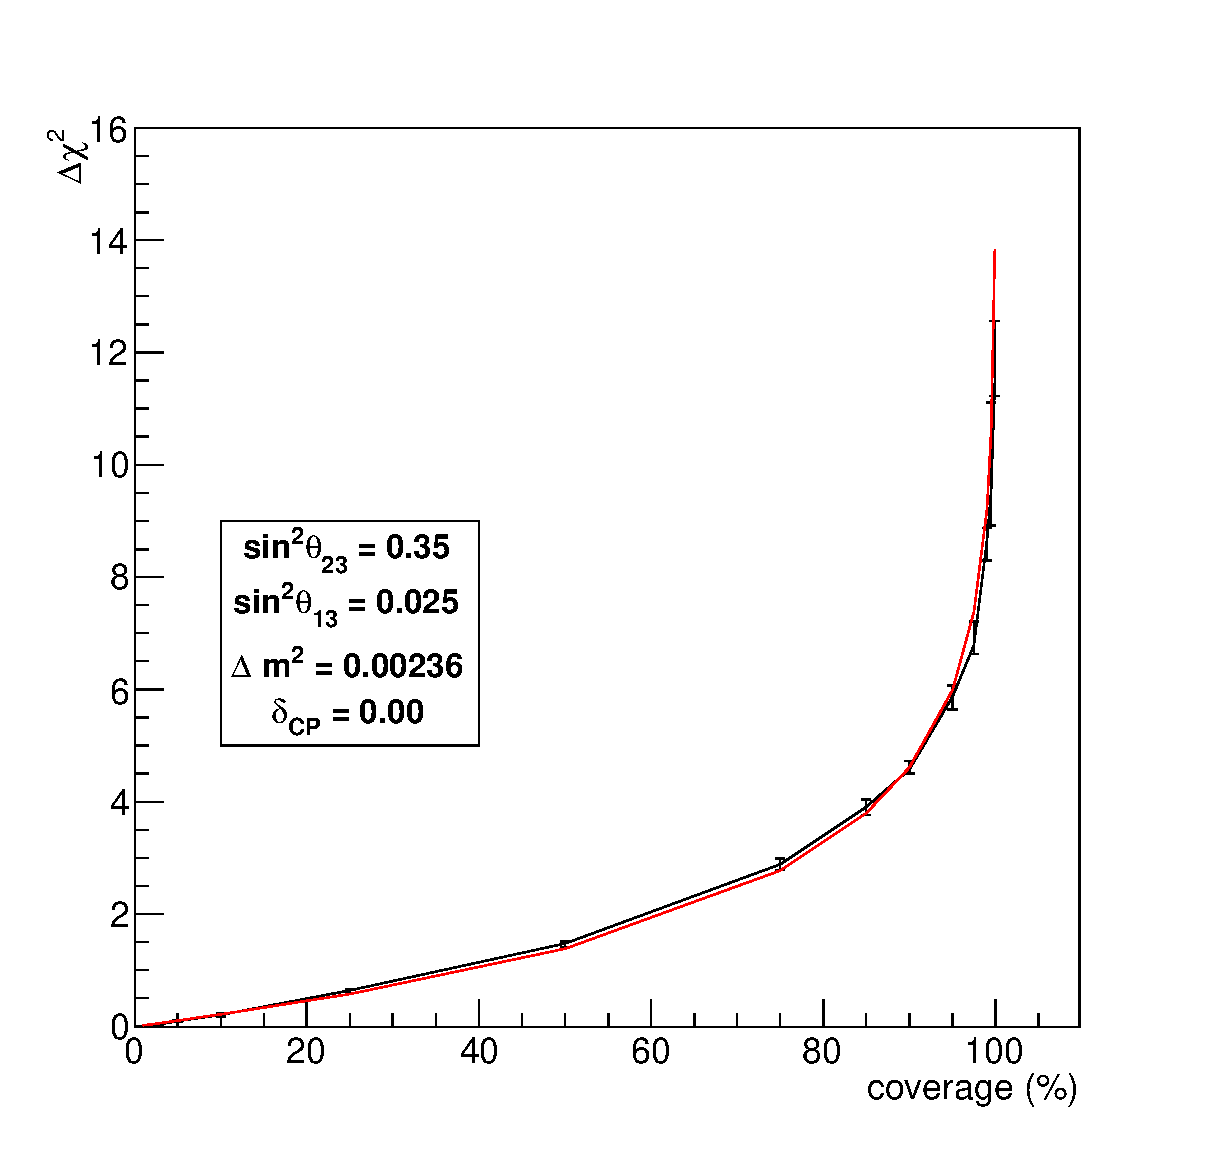
\includegraphics[width=14pc]{./images/appendix/coverage/coverage_study_2D_theta23_dm23sq_syst_0.eps}
%\center
%\caption {
  %Distribution of $\Delta\chi^{2}$ vs coverage in the ($sin^{2}\theta_{23}$,$|\Delta m^{2}|$) parameter space
  %from 1k toy MC experiments generated with the Run 1+2+3 POT
 % with statistical fluctuations and systematic variations at the oscillation point: 
 % $|\Delta m^{2}| = 2.36 \times 10^{-3}$,
%  $sin^{2}\theta_{23} = 0.35$,
  %$sin^{2}\theta_{13} = 0.025$ and
  %	$\delta_{CP}$	= 0.
%}
%\label{fig:cov_2D_theta23_dmsq_syst_0}
%\end{minipage}
%\hspace{0.03\linewidth}
%\begin{minipage}[t]{0.46\linewidth}
%\center
%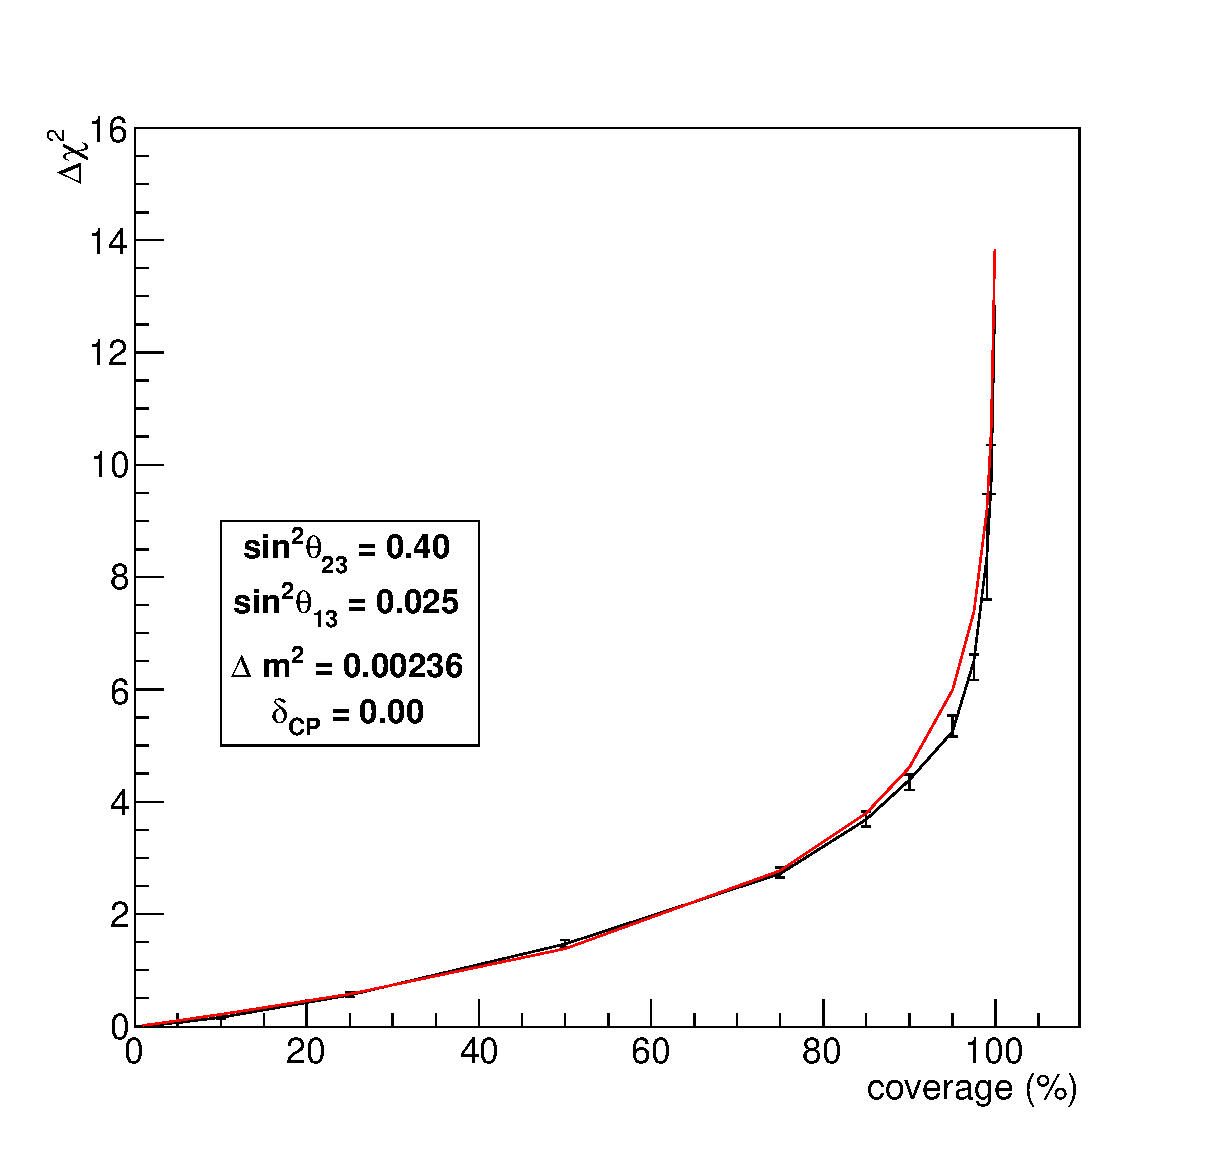
\includegraphics[width=14pc]{./images/appendix/coverage/coverage_study_2D_theta23_dm23sq_syst_1.eps}
%\center
%\caption {
%   Distribution of $\Delta\chi^{2}$ vs coverage in the ($sin^{2}\theta_{23}$,$|\Delta m^{2}|$) parameter space
%  from 1k toy MC experiments generated with the Run 1+2+3 POT
% with statistical fluctuations and systematic variations at the oscillation point: 
%  $|\Delta m^{2}| = 2.36 \times 10^{-3}$,
%  $sin^{2}\theta_{23} = 0.4$,
%  $sin^{2}\theta_{13} = 0.025$ and
%  	$\delta_{CP}$	= 0.
%	}
%\label{fig:cov_2D_theta23_dmsq_syst_1}
%\end{minipage}
%\vfill
%\vspace*{0.7cm}
%\begin{minipage}[t]{0.46\linewidth}
%\center
%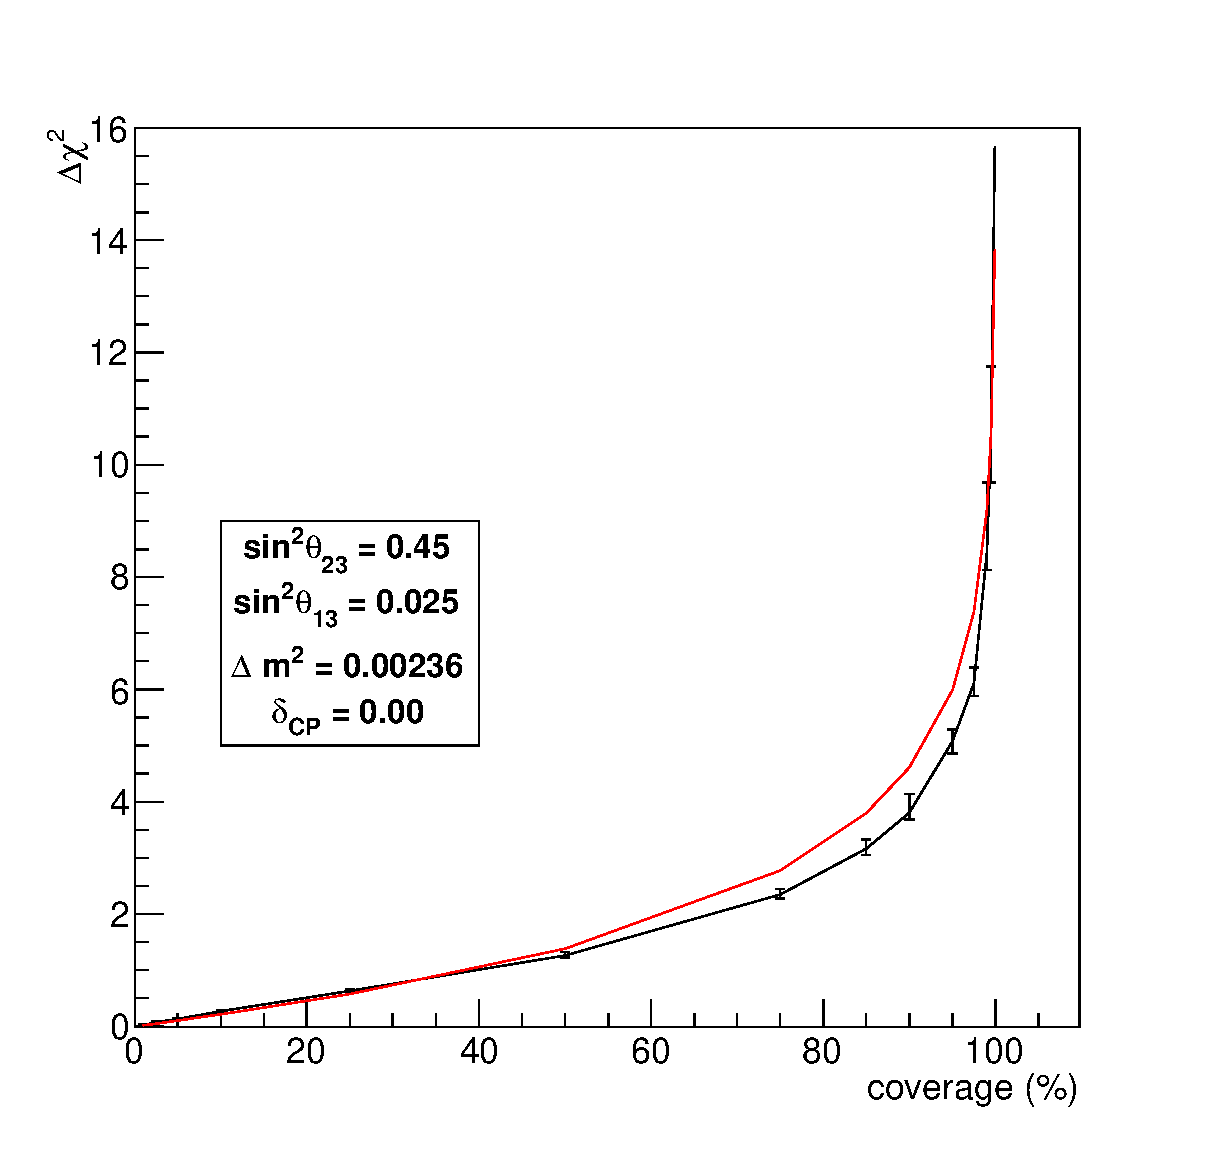
\includegraphics[width=14pc]{./images/appendix/coverage/coverage_study_2D_theta23_dm23sq_syst_2.eps}
%\center
%\caption {
%   Distribution of $\Delta\chi^{2}$ vs coverage in the ($sin^{2}\theta_{23}$,$|\Delta m^{2}|$) parameter space
%  from 1k toy MC experiments generated with the Run 1+2+3 POT
% with statistical fluctuations and systematic variations at the oscillation point: 
%  $|\Delta m^{2}| = 2.36 \times 10^{-3}$,
%  $sin^{2}\theta_{23} = 0.45$,
%  $sin^{2}\theta_{13} = 0.025$ and
%  	$\delta_{CP}$	= 0.
%	}
%\label{fig:cov_2D_theta23_dmsq_syst_2}
%\end{minipage}
%\hspace{0.03\linewidth}
%\begin{minipage}[t]{0.46\linewidth}
%\center
%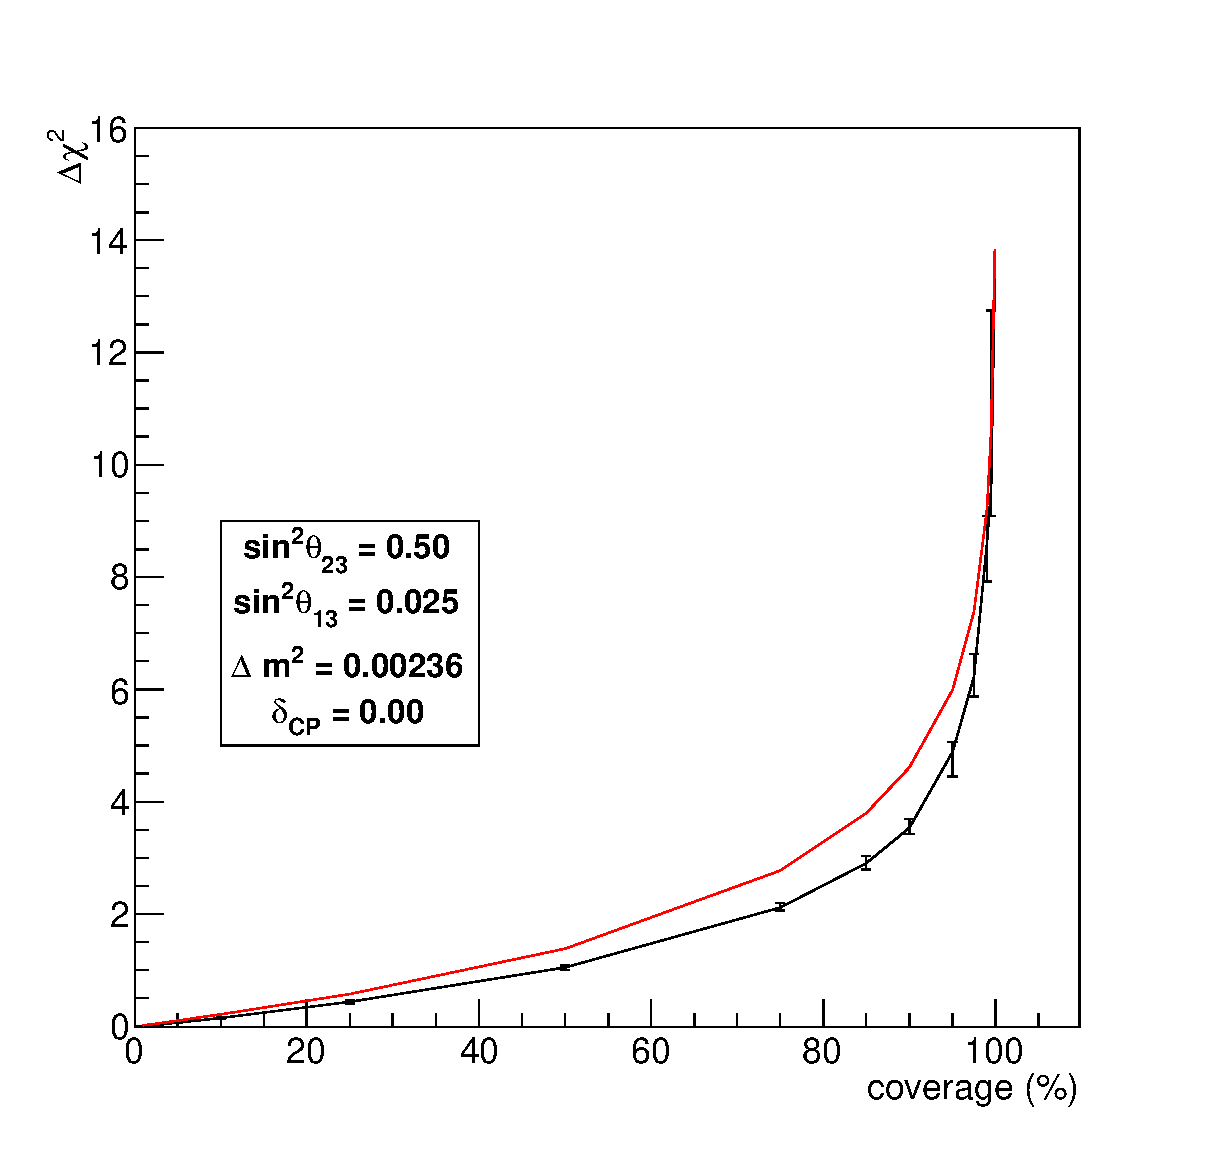
\includegraphics[width=14pc]{./images/appendix/coverage/coverage_study_2D_theta23_dm23sq_syst_3.eps}
%\center
%\caption {
%   Distribution of $\Delta\chi^{2}$ vs coverage in the ($sin^{2}\theta_{23}$,$|\Delta m^{2}|$) parameter space
%  from 1k toy MC experiments generated with the Run 1+2+3 POT
% with statistical fluctuations and systematic variations at the oscillation point: 
%  $|\Delta m^{2}| = 2.36 \times 10^{-3}$,
%  $sin^{2}\theta_{23} = 0.5$,
%  $sin^{2}\theta_{13} = 0.025$ and
%  	$\delta_{CP}$	= 0.
%	}
%\label{fig:cov_2D_theta23_dmsq_syst_3}
%\end{minipage}
%\vfill
%\vspace*{0.7cm}
%\center


%\end{figure*}
%\end{center}



%% FIGURES FOR 2D theta13-dmsq

%\begin{center}
%\begin{figure*}[htb]
%\begin{minipage}[t]{0.46\linewidth}
%\center
%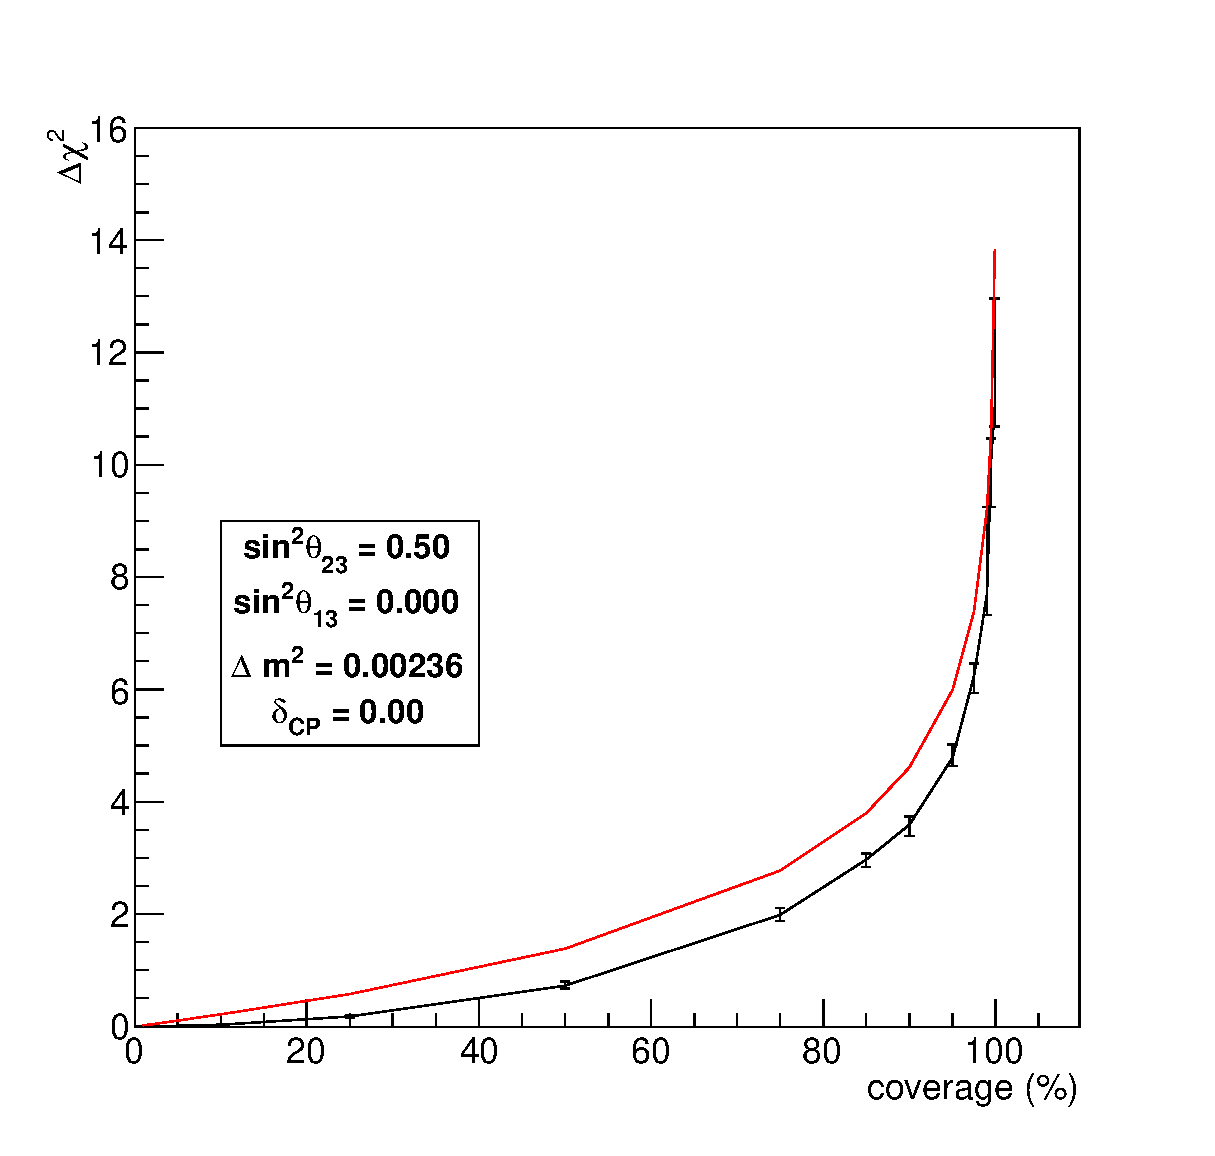
\includegraphics[width=14pc]{./images/appendix/coverage/coverage_study_2D_theta13_dm23sq_syst_0.eps}
%\center
%\caption {
  %Distribution of $\Delta\chi^{2}$ vs coverage in the ($sin^{2}\theta_{13}$,$|\Delta m^{2}|$) parameter space
  %from 1k toy MC experiments generated with the Run 1+2+3 POT
% with statistical fluctuations and systematic variations at the oscillation point: 
%  $|\Delta m^{2}| = 2.36 \times 10^{-3}$,
%  $sin^{2}\theta_{23} = 0.5$,
%  $sin^{2}\theta_{13} = 0.0$ and
%  	$\delta_{CP}$	= 0.
%}
%\label{fig:cov_2D_theta13_dm23sq_syst_0}
%\end{minipage}
%\hspace{0.03\linewidth}
%\begin{minipage}[t]{0.46\linewidth}
%\center
%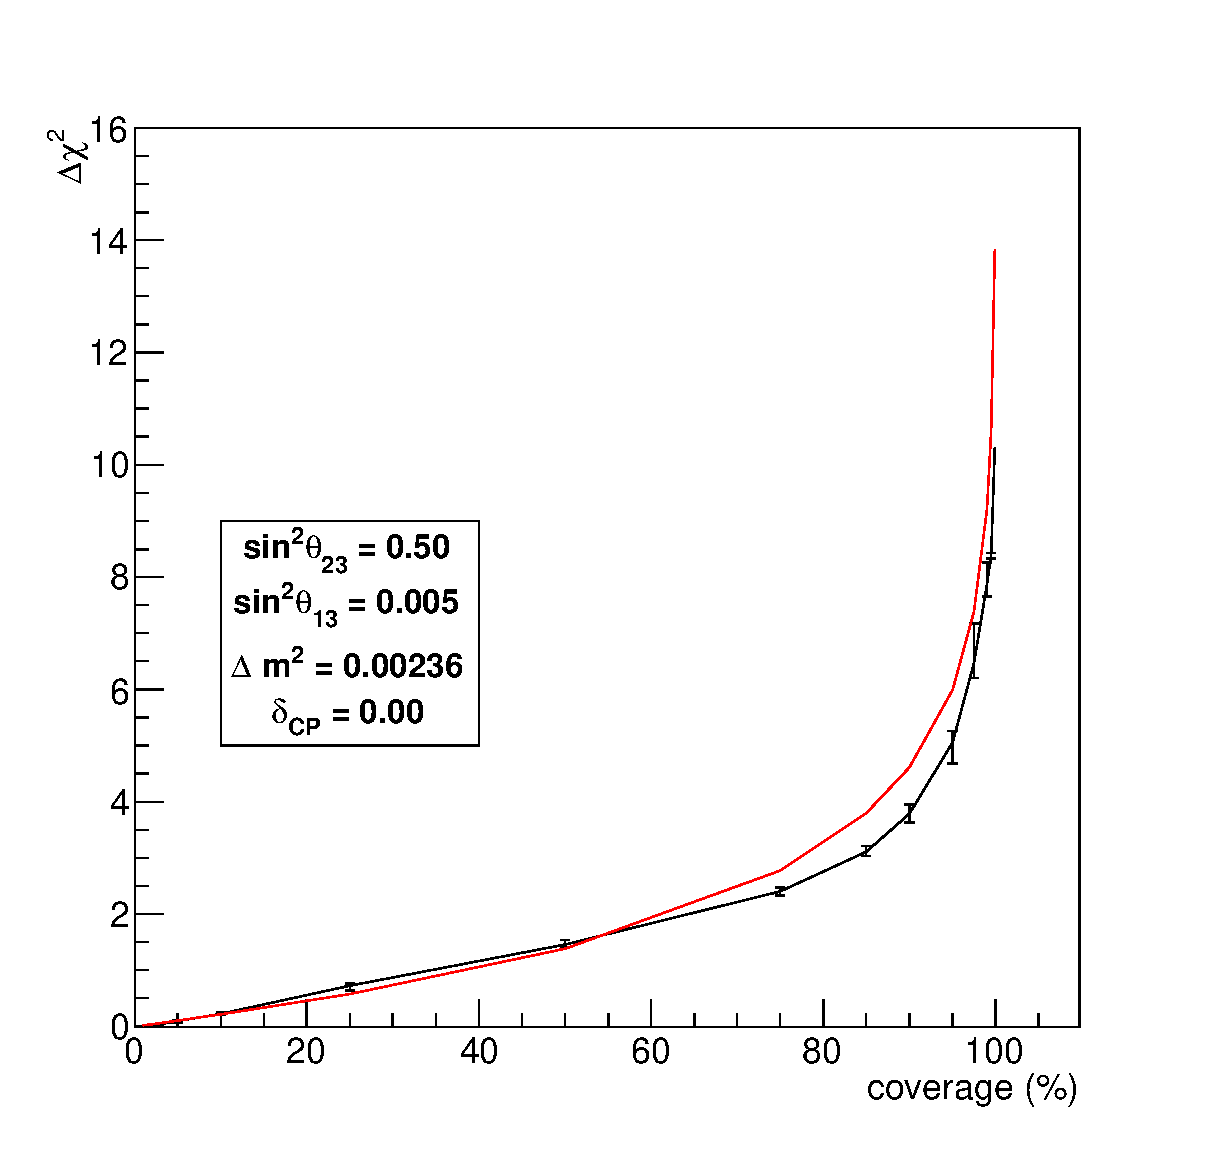
\includegraphics[width=14pc]{./images/appendix/coverage/coverage_study_2D_theta13_dm23sq_syst_1.eps}
%\center
%\caption {
%   Distribution of $\Delta\chi^{2}$ vs coverage in the ($sin^{2}\theta_{13}$,$|\Delta m^{2}|$) parameter space
%  from 1k toy MC experiments generated with the Run 1+2+3 POT
%  with statistical fluctuations and systematic variations at the oscillation point: 
%  $|\Delta m^{2}| = 2.36 \times 10^{-3}$,
%  $sin^{2}\theta_{23} = 0.5$,
%  $sin^{2}\theta_{13} = 0.005$ and
%  	$\delta_{CP}$	= 0.
%	}
%\label{fig:cov_2D_theta13_dm23sq_syst_1}
%\end{minipage}
%\vfill
%\vspace*{0.7cm}
%\begin{minipage}[t]{0.46\linewidth}
%\center
%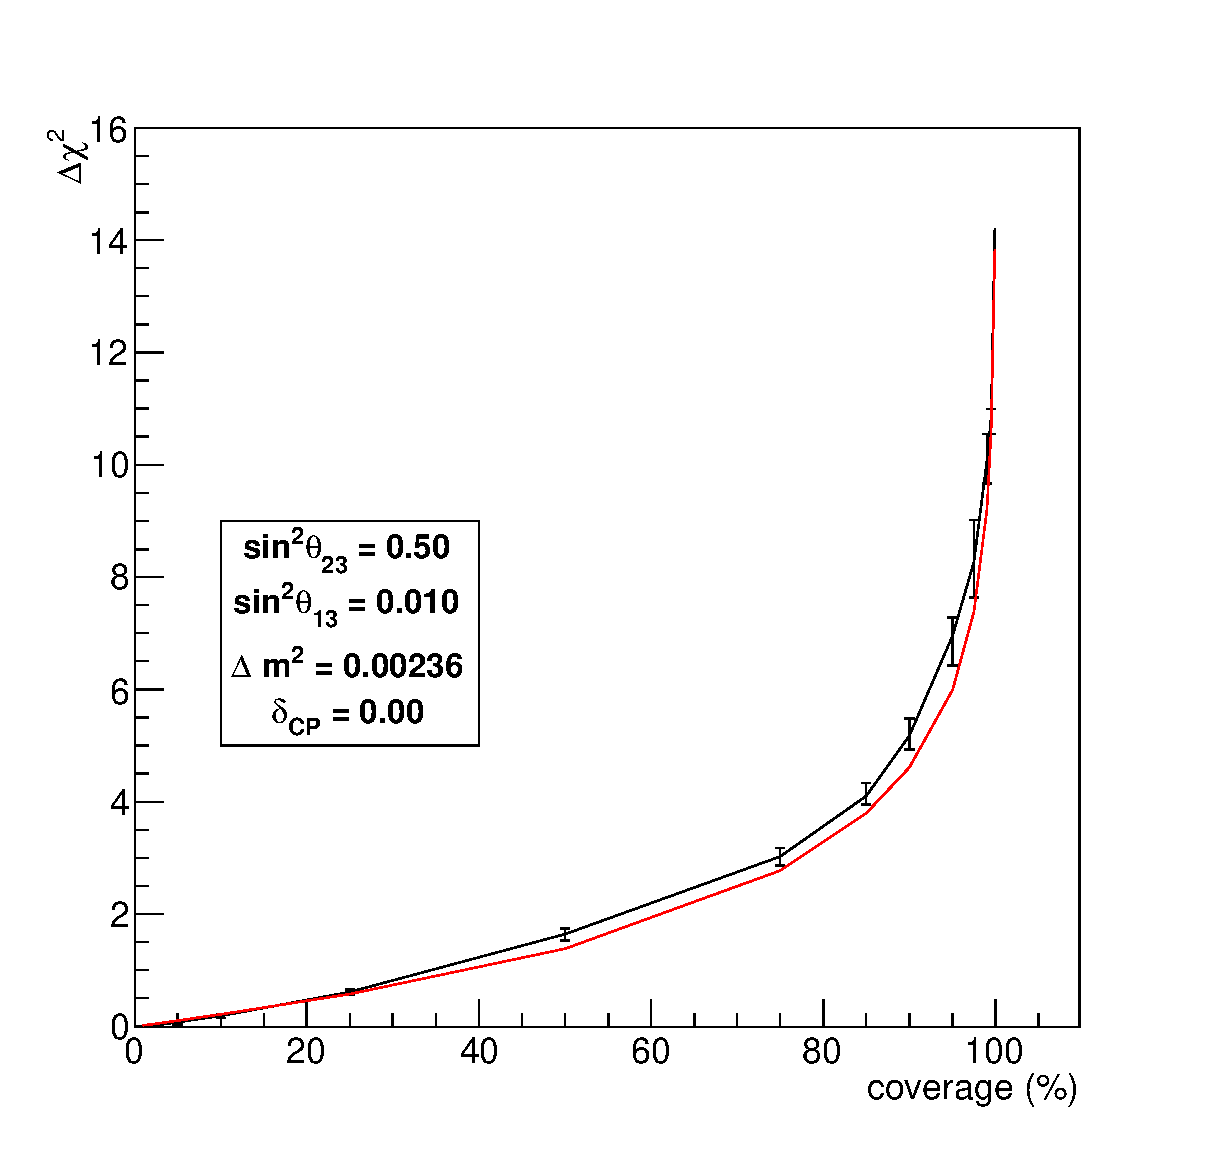
\includegraphics[width=14pc]{./images/appendix/coverage/coverage_study_2D_theta13_dm23sq_syst_2.eps}
%\center
%\caption {
%   Distribution of $\Delta\chi^{2}$ vs coverage in the ($sin^{2}\theta_{13}$,$|\Delta m^{2}|$) parameter space
%  from 1k toy MC experiments generated with the Run 1+2+3 POT
% with statistical fluctuations and systematic variations at the oscillation point: 
%  $|\Delta m^{2}| = 2.36 \times 10^{-3}$,
%  $sin^{2}\theta_{23} = 0.5$,
%  $sin^{2}\theta_{13} = 0.01$ and
%  	$\delta_{CP}$	= 0.
%	}
%\label{fig:cov_2D_theta13_dm23sq_syst_2}
%\end{minipage}
%\hspace{0.03\linewidth}
%\begin{minipage}[t]{0.46\linewidth}
%\center
%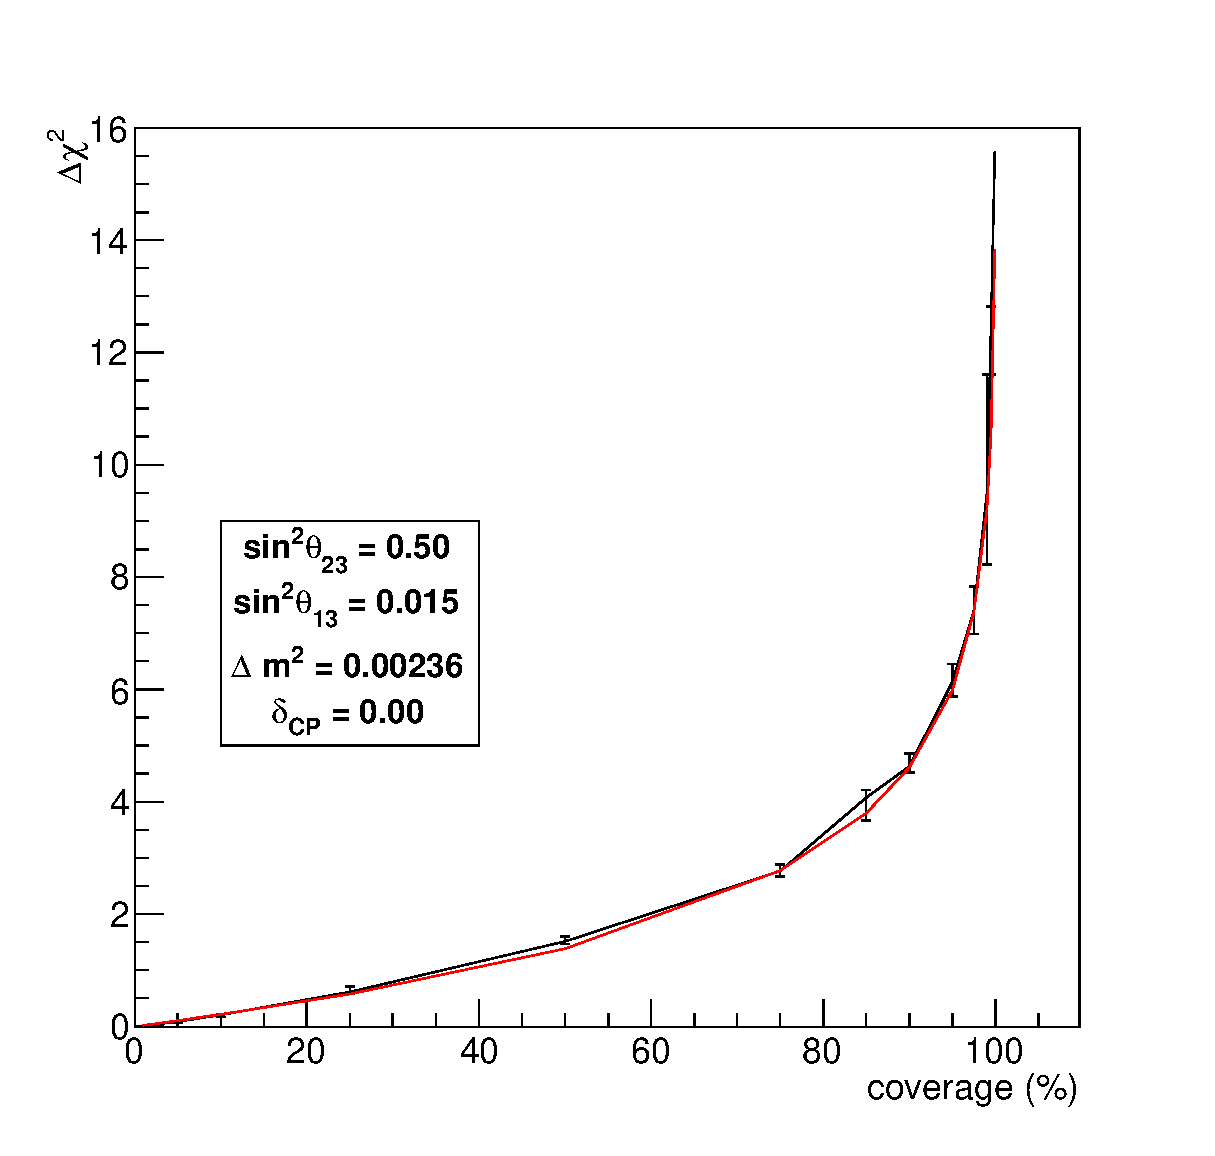
\includegraphics[width=14pc]{./images/appendix/coverage/coverage_study_2D_theta13_dm23sq_syst_3.eps}
%\center
%\caption {
%   Distribution of $\Delta\chi^{2}$ vs coverage in the ($sin^{2}\theta_{13}$,$|\Delta m^{2}|$) parameter space
%  from 1k toy MC experiments generated with the Run 1+2+3 POT
%   with statistical fluctuations and systematic variations at the oscillation point: 
%  $|\Delta m^{2}| = 2.36 \times 10^{-3}$,
%  $sin^{2}\theta_{23} = 0.5$,
%  $sin^{2}\theta_{13} = 0.015$ and
%  	$\delta_{CP}$	= 0.
%	}
%\label{fig:cov_2D_theta13_dm23sq_syst_3}
%\end{minipage}
%\vfill
%\vspace*{0.7cm}
%\begin{minipage}[t]{0.46\linewidth}
%\center
%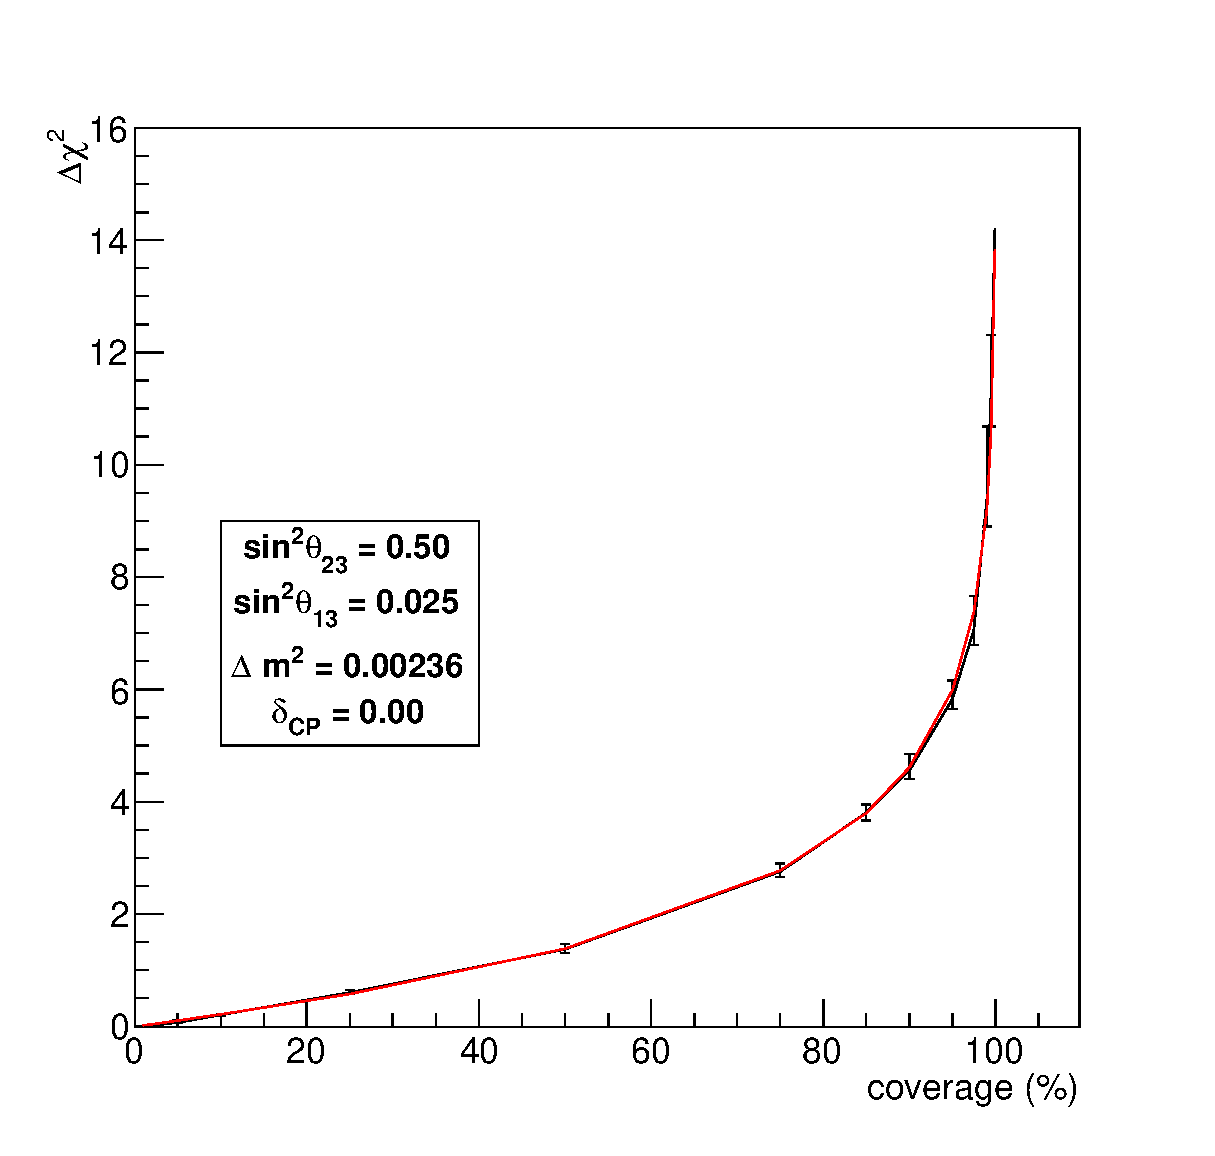
\includegraphics[width=14pc]{./images/appendix/coverage/coverage_study_2D_theta13_dm23sq_syst_4.eps}
%\center
%\caption {
%   Distribution of $\Delta\chi^{2}$ vs coverage in the ($sin^{2}\theta_{13}$,$|\Delta m^{2}|$) parameter space
%  from 1k toy MC experiments generated with the Run 1+2+3 POT
% with statistical fluctuations and systematic variations at the oscillation point: 
%  $|\Delta m^{2}| = 2.36 \times 10^{-3}$,
%  $sin^{2}\theta_{23} = 0.5$,
%  $sin^{2}\theta_{13} = 0.025$ and
%  	$\delta_{CP}$	= 0.
%	}
%\label{fig:cov_2D_theta13_dm23sq_syst_4}
%\end{minipage}
\begin{center}
\begin{figure*}[htb]
\begin{minipage}[t]{0.46\linewidth}
\center
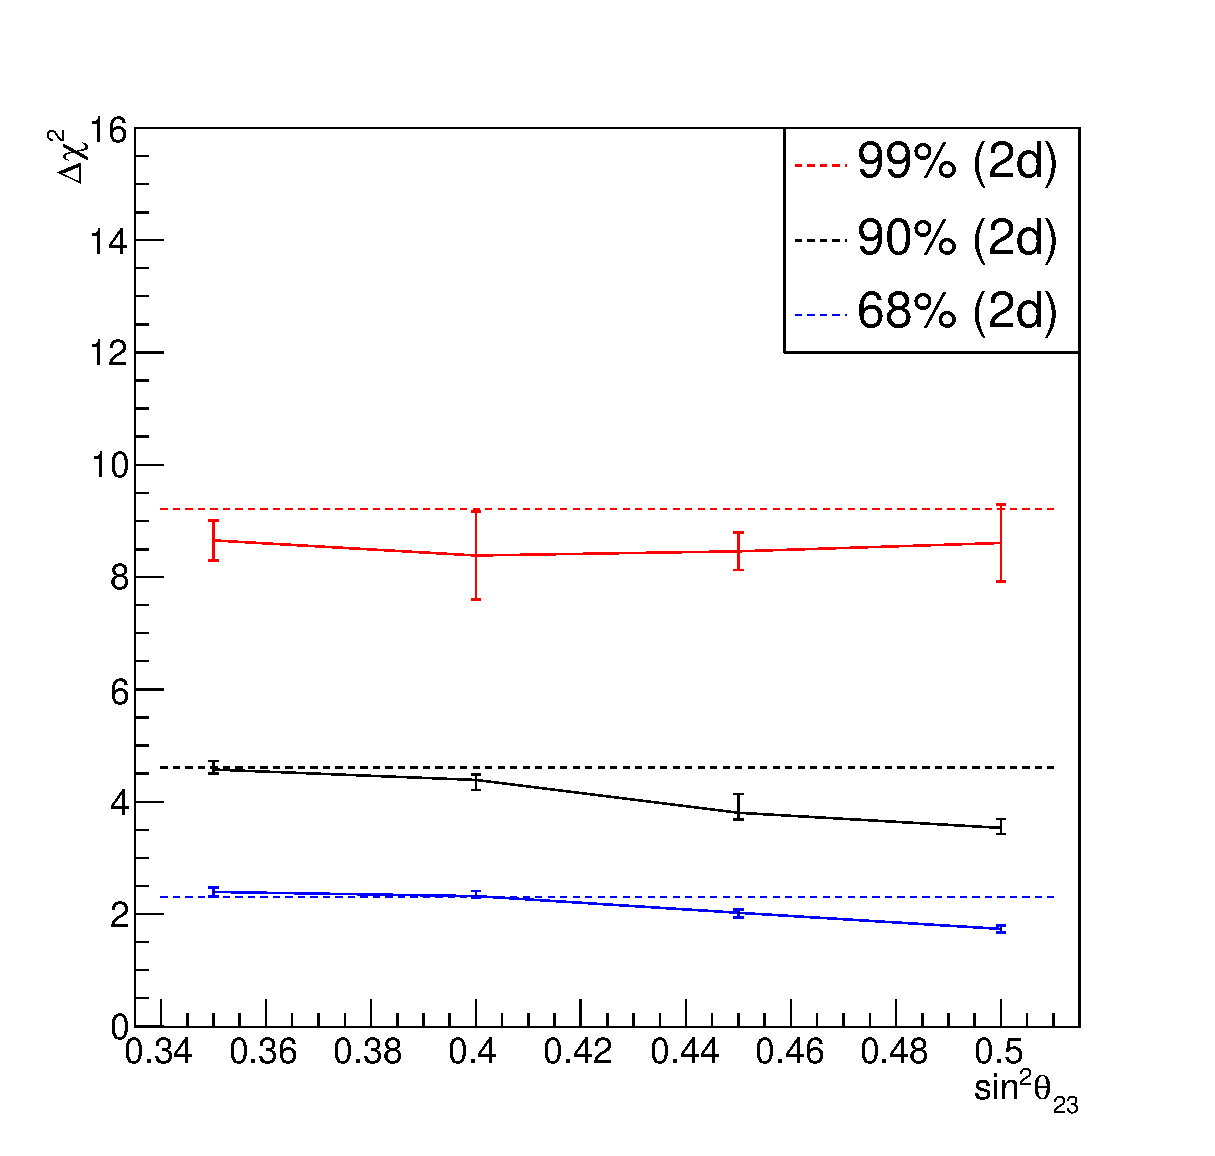
\includegraphics[width=14pc]{./images/appendix/coverage/coverage_study_2D_theta23_dm23sq_syst_all.eps}
\caption {
   Summary of values of $\Delta\chi^{2}$ at 99\%, 90\% and 68\% confidence intervals in the 2D parameter space ($sin^{2}\theta_{23}$,$|\Delta m^{2}|$) vs the value of $sin^{2}\theta_{23}$. 
True input values for the other oscillation parameters:
$|\Delta m^{2}| = 2.36 \times 10^{-3}$,
  $sin^{2}\theta_{13} = 0.025$ and
        $\delta_{CP}$   = 0.
	}
\label{fig:cov_2D_theta23_dmsq_syst_all}
\end{minipage}
\hspace{0.03\linewidth}
\begin{minipage}[t]{0.46\linewidth}
\center
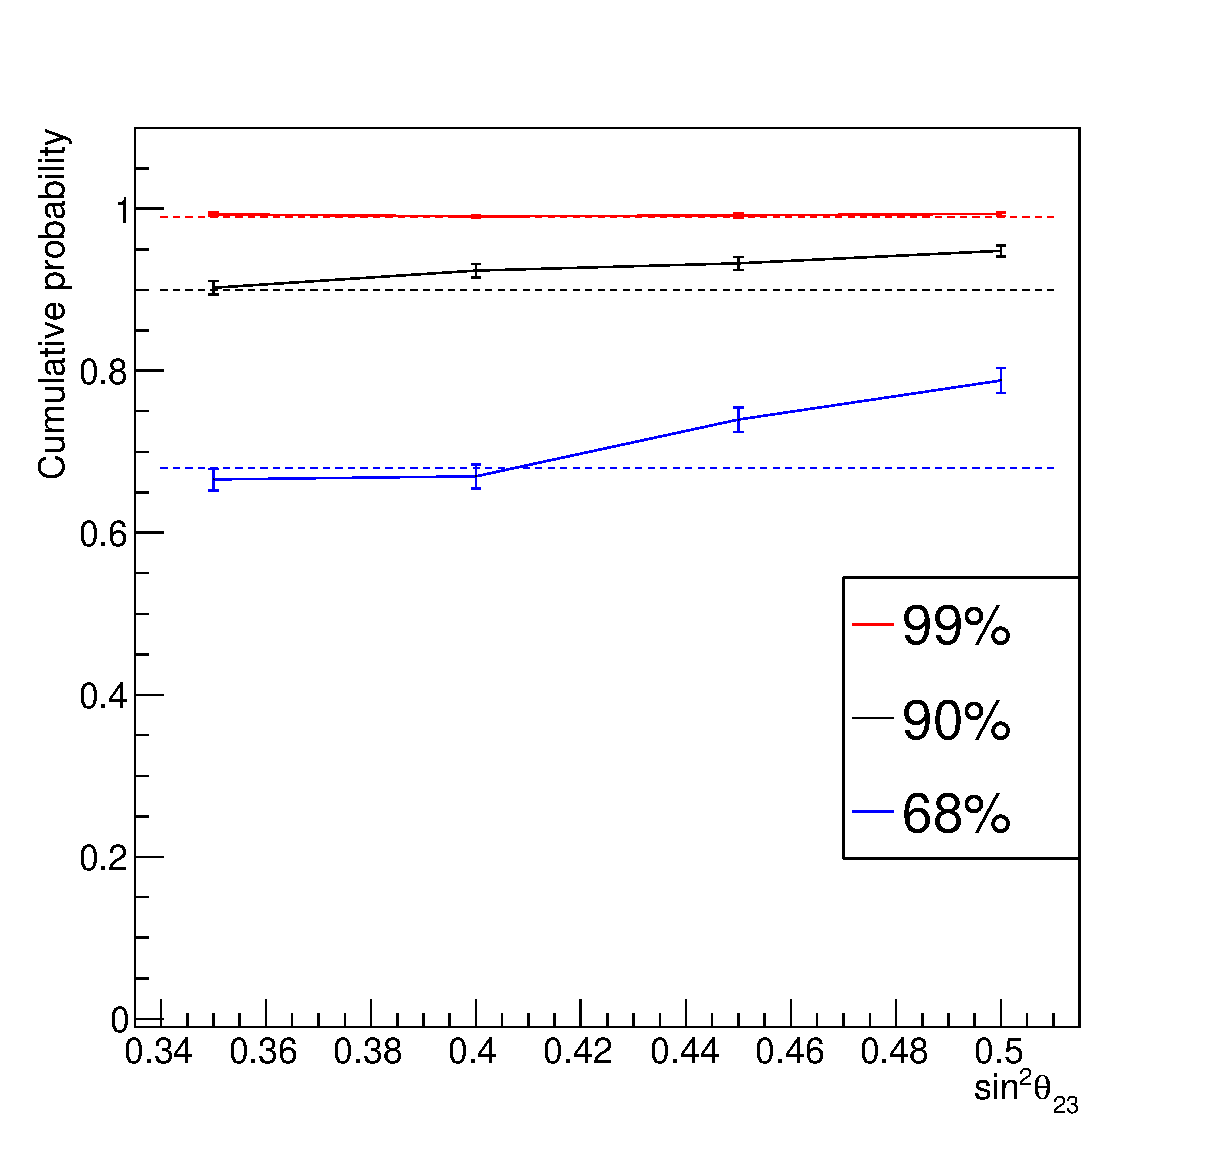
\includegraphics[width=14pc]{./images/appendix/coverage/coverage_study_2D_syst_theta23_dmsq_new_all.eps}
\caption {
   Summary of values of cumulative probability  for $\Delta\chi^{2}=9.21$ (canonical value for 99\%), $\Delta\chi^{2}=4.61$ (canonical value for 90\%) and $\Delta\chi^{2}=2.30$ (canonical value for 68\%) in the 2D parameter space ($sin^{2}\theta_{23}$,$|\Delta m^{2}|$) vs the value of $sin^{2}\theta_{23}$. 
True input values for the other oscillation parameters:
$|\Delta m^{2}| = 2.36 \times 10^{-3}$,
  $sin^{2}\theta_{13} = 0.025$ and
        $\delta_{CP}$   = 0.
	}
\label{fig:prob_2D_theta23_dmsq_syst_all}
\end{minipage}
\vfill
\vspace*{0.7cm}
\begin{minipage}[t]{0.46\linewidth}
\center
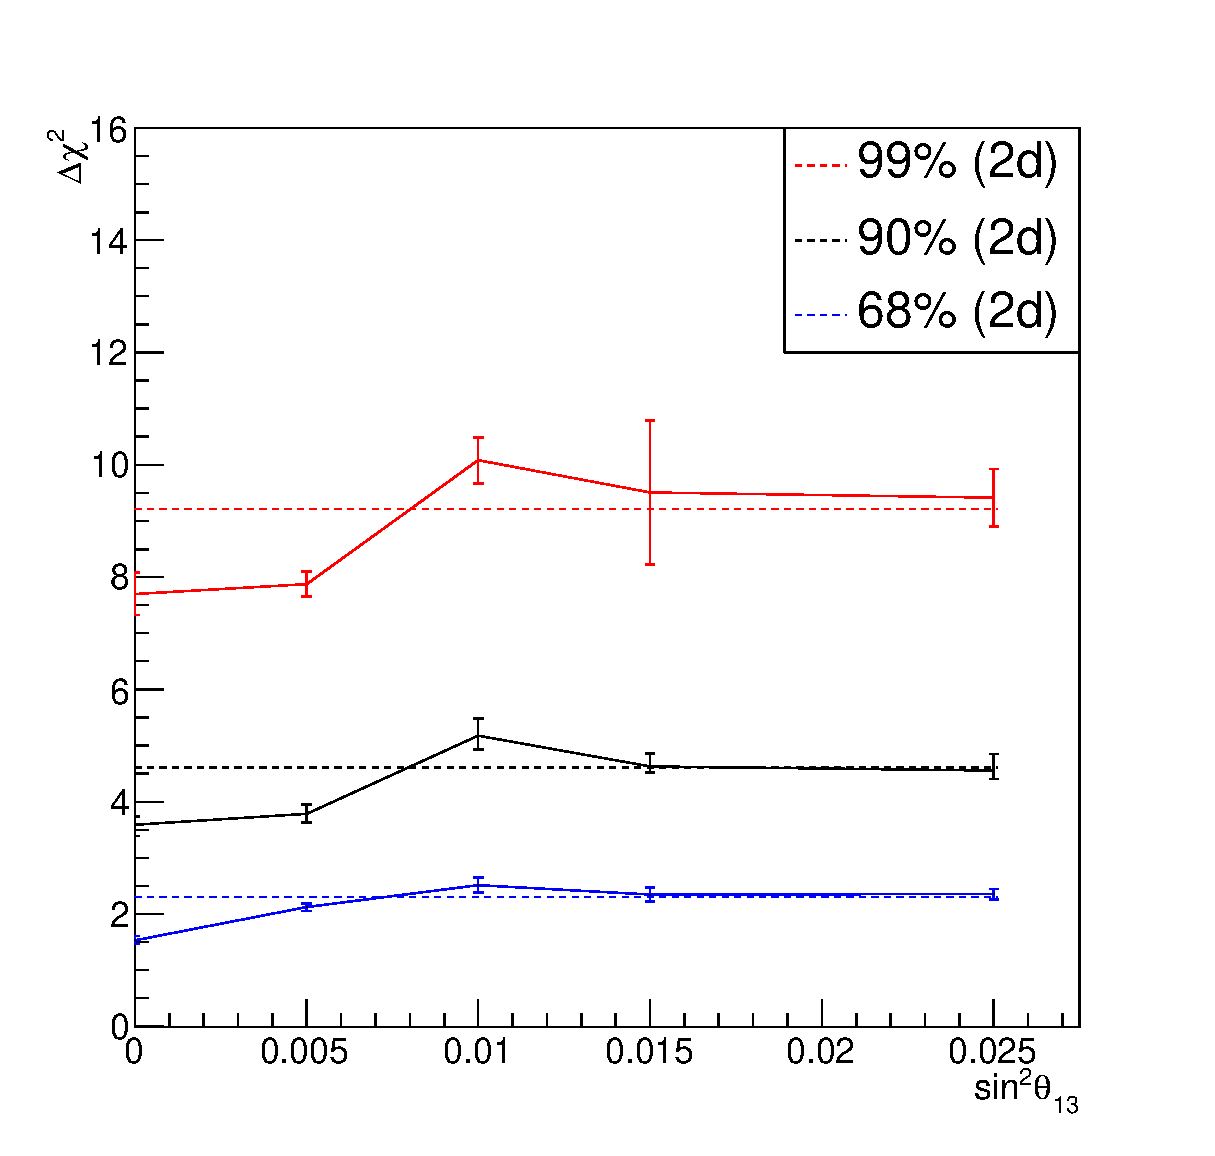
\includegraphics[width=14pc]{./images/appendix/coverage/coverage_study_2D_theta13_dm23sq_syst_all.eps}
\center
\caption {
   Summary of values of $\Delta\chi^{2}$ at 99\%, 90\% and 68\% confidence intervals in the 2D parameter space ($sin^{2}\theta_{13}$,$|\Delta m^{2}|$) vs the value of $sin^{2}\theta_{13}$.
True input values for the other oscillation parameters:
$|\Delta m^{2}| = 2.36 \times 10^{-3}$,
  $sin^{2}\theta_{23} = 0.5$ and
        $\delta_{CP}$   = 0.
	}
\label{fig:cov_2D_theta13_dmsq_syst_all}
\end{minipage}
\hspace{0.03\linewidth}
\begin{minipage}[t]{0.46\linewidth}
\center
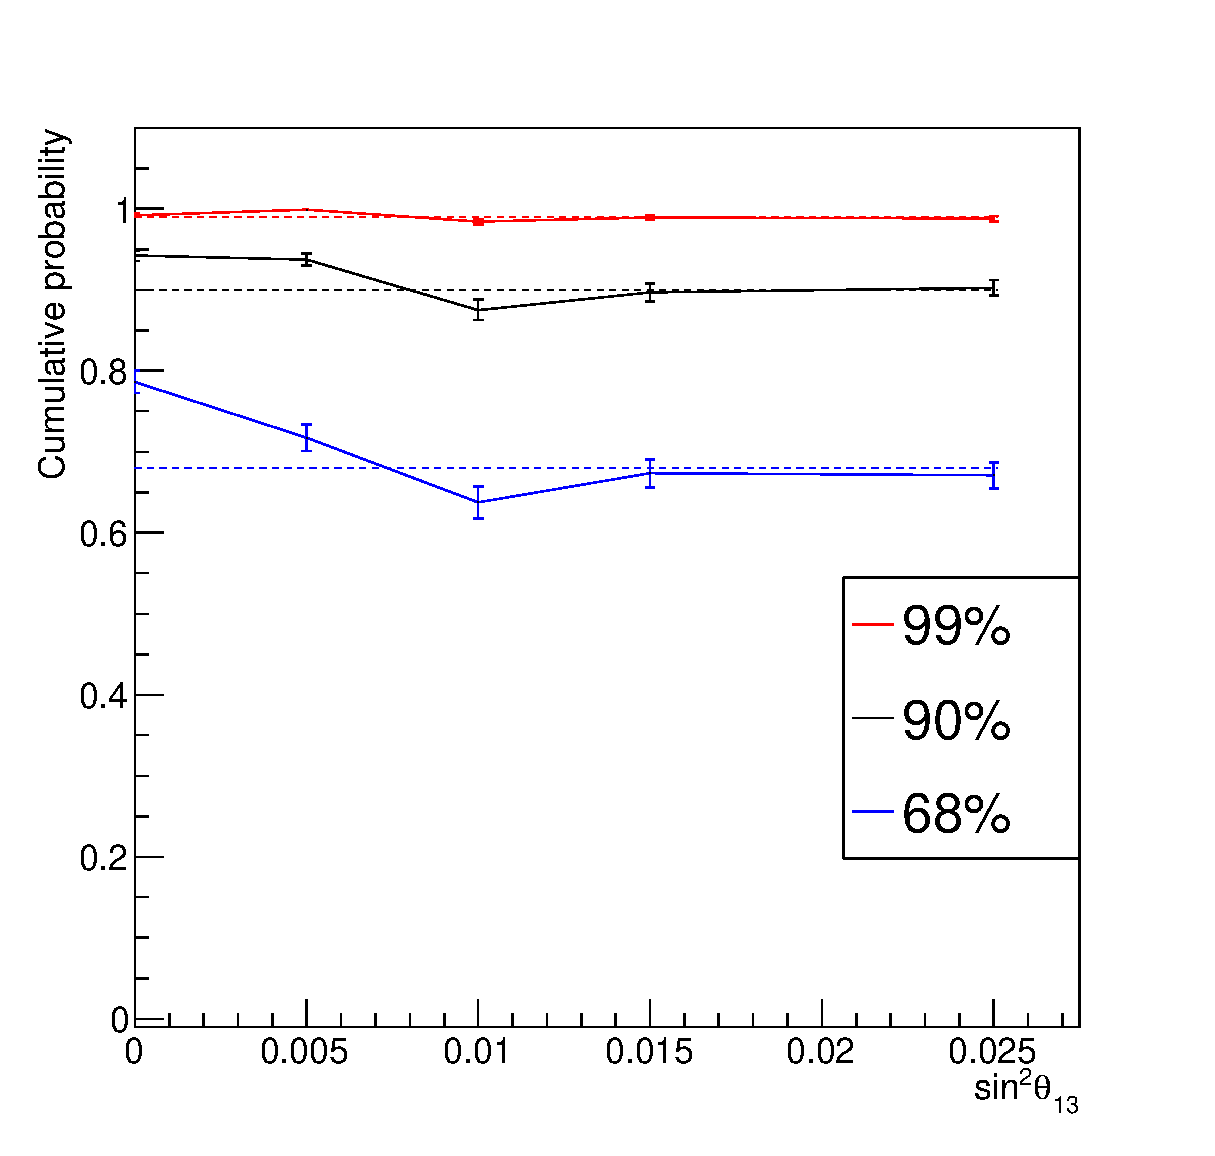
\includegraphics[width=14pc]{./images/appendix/coverage/coverage_study_2D_syst_theta13_dmsq_new_all.eps}
\caption {
   Summary of values of cumulative probability  for $\Delta\chi^{2}=9.21$ (canonical value for 99\%), $\Delta\chi^{2}=4.61$ (canonical value for 90\%) and $\Delta\chi^{2}=2.30$ (canonical value for 68\%) in the 2D parameter space ($sin^{2}\theta_{13}$,$|\Delta m^{2}|$) vs the value of $sin^{2}\theta_{13}$. 
True input values for the other oscillation parameters:
$|\Delta m^{2}| = 2.36 \times 10^{-3}$,
  $sin^{2}\theta_{23} = 0.5$ and
        $\delta_{CP}$   = 0.
	}
\label{fig:prob_2D_theta13_dmsq_syst_all}
\end{minipage}
\vfill
\vspace*{0.7cm}
\center
\begin{minipage}[t]{0.46\linewidth}
\center
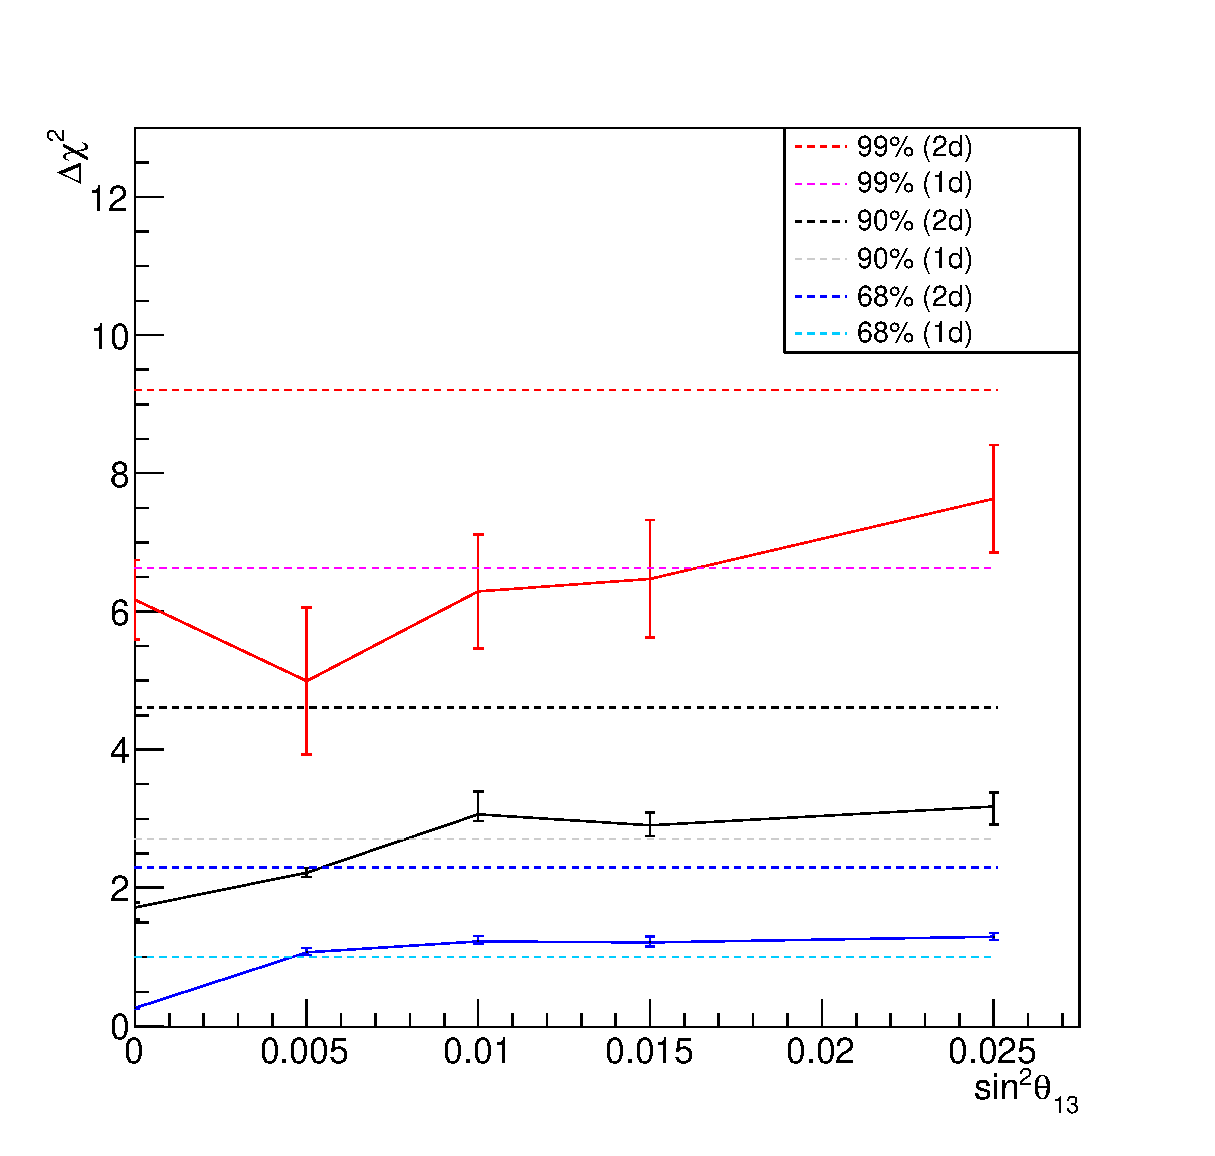
\includegraphics[width=14pc]{./images/appendix/coverage/coverage_study_2D_theta13_deltacp_syst_all.eps}
\caption {
   Summary of values of $\Delta\chi^{2}$ at 99\%, 90\% and 68\% confidence intervals in the 2D parameter space ($sin^{2}\theta_{13}$,$|\delta_{CP}|$) vs the value of $sin^{2}\theta_{13}$.
True input values for the other oscillation parameters:
$|\Delta m^{2}| = 2.36 \times 10^{-3}$,
  $sin^{2}\theta_{23} = 0.5$ and
        $\delta_{CP}$   = 0.
	}
\label{fig:cov_2D_theta13_deltacp_syst_all}
\end{minipage}
\hspace{0.03\linewidth}
\begin{minipage}[t]{0.46\linewidth}
\center
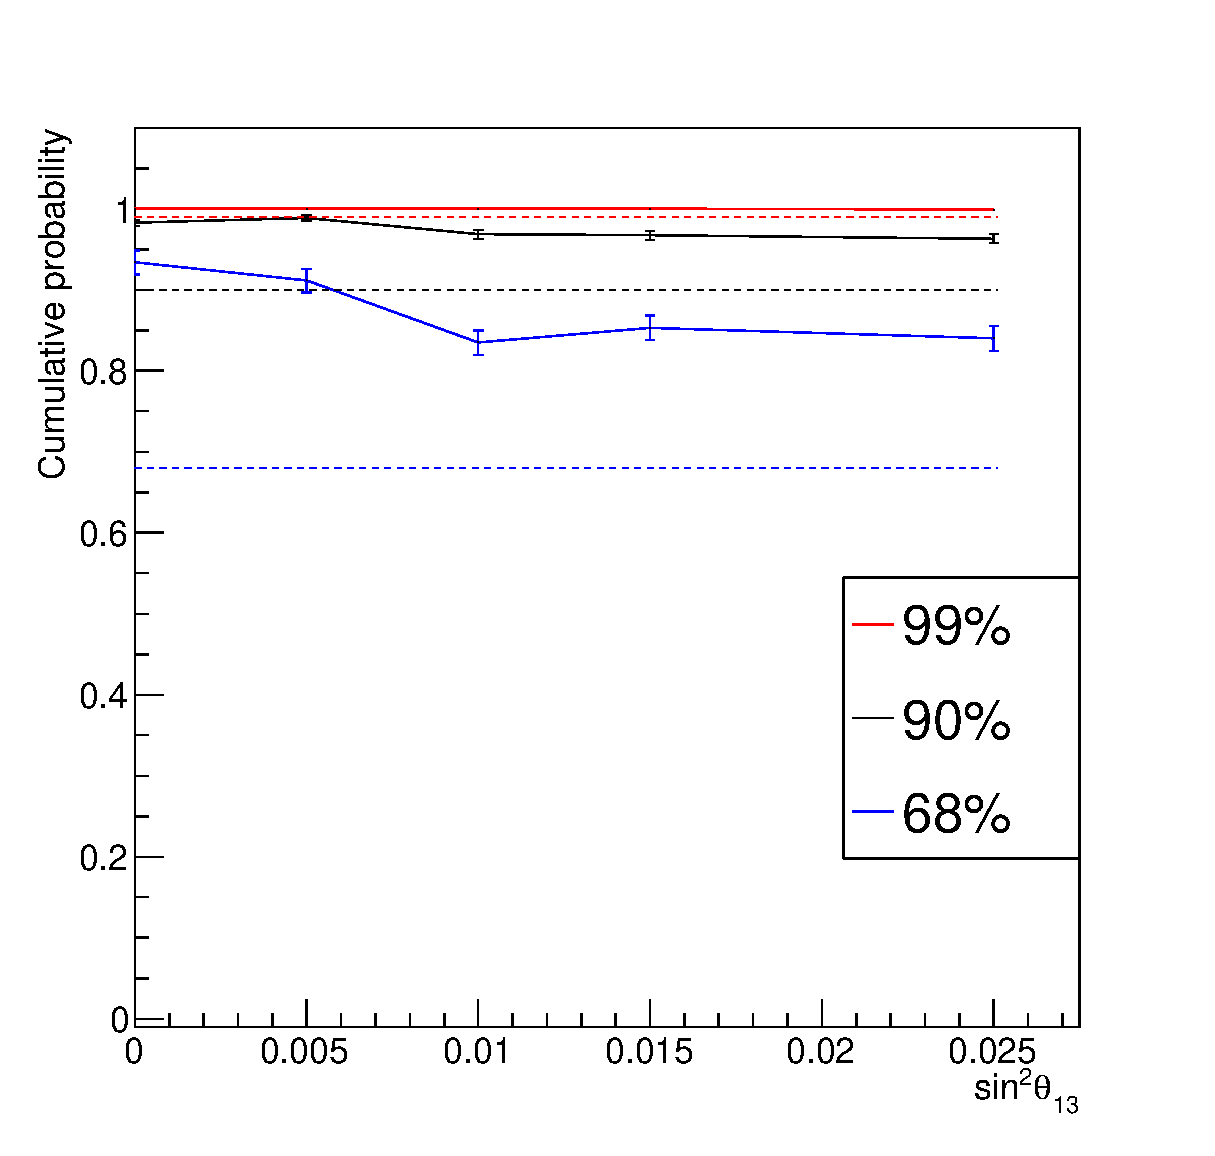
\includegraphics[width=14pc]{./images/appendix/coverage/coverage_study_2D_syst_theta13_deltacp_new_all.eps}
\caption {
   Summary of values of cumulative probability  for $\Delta\chi^{2}=9.21$ (canonical value for 99\%), $\Delta\chi^{2}=4.61$ (canonical value for 90\%) and $\Delta\chi^{2}=2.30$ (canonical value for 68\%) in the 2D parameter space ($sin^{2}\theta_{13}$,$\delta_{CP}$) vs the value of $sin^{2}\theta_{13}$. 
True input values for the other oscillation parameters:
$|\Delta m^{2}| = 2.36 \times 10^{-3}$,
  $sin^{2}\theta_{23} = 0.5$ and
        $\delta_{CP}$   = 0.
	}
\label{fig:prob_2D_theta13_deltacp_syst_all}
\end{minipage}
\end{figure*}
\end{center}


%% FIGURES FOR 2D theta13-dmsq

%\begin{center}
%\begin{figure*}[htb]
%\begin{minipage}[t]{0.46\linewidth}
%\center
%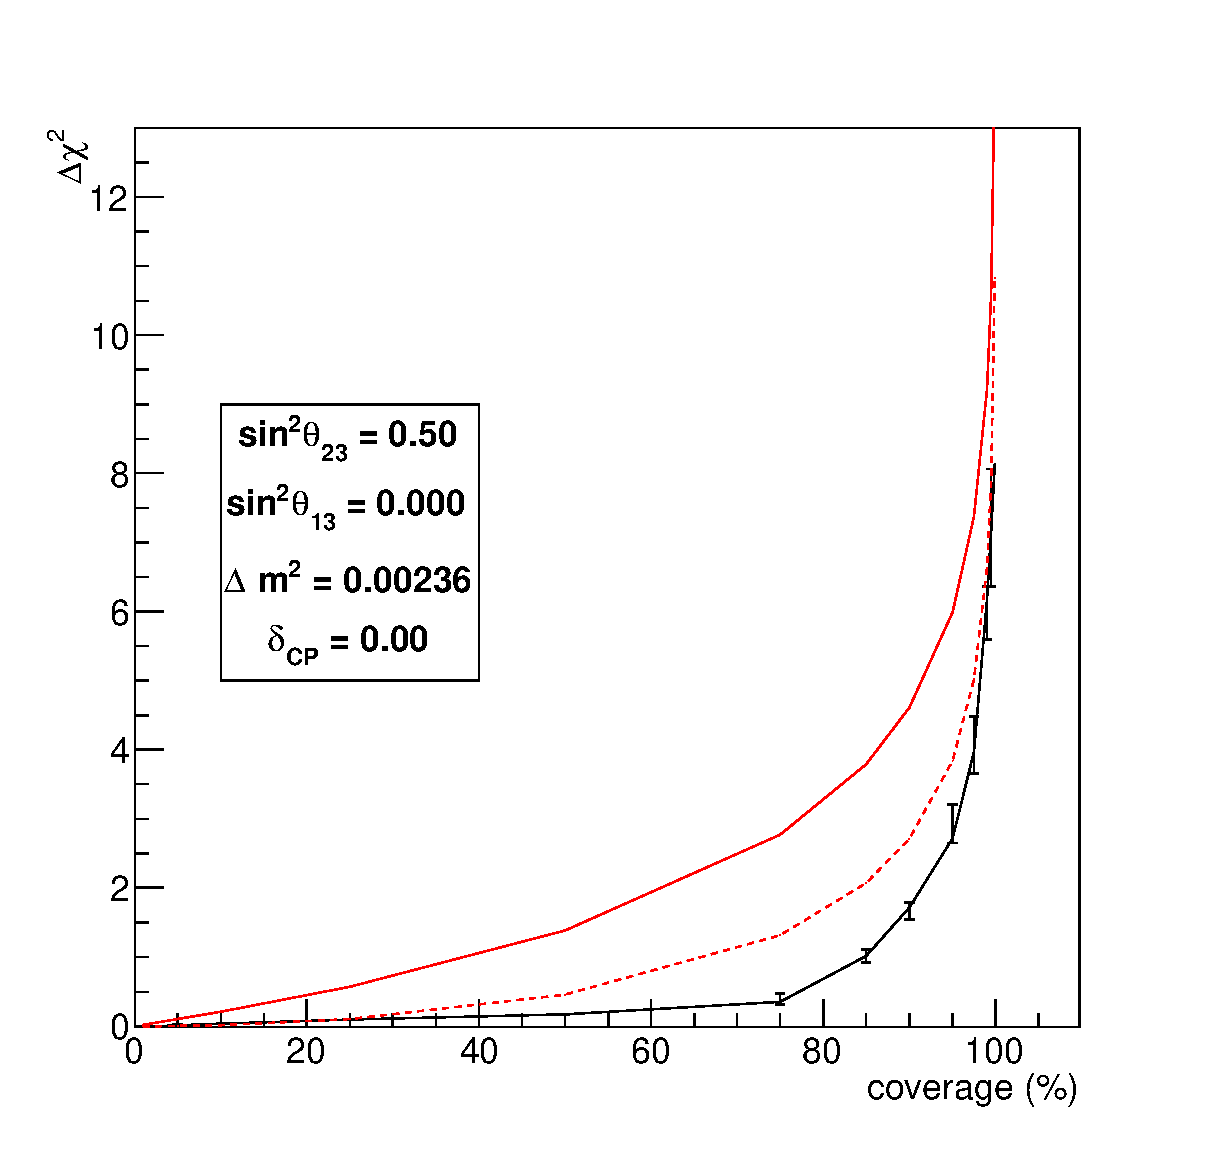
\includegraphics[width=14pc]{./images/appendix/coverage/coverage_study_2D_theta13_deltacp_syst_0.eps}
%\center
%\caption {
%  Distribution of $\Delta\chi^{2}$ vs coverage in the ($sin^{2}\theta_{13}$,$\delta_{CP}$) parameter space
%  from 1k toy MC experiments generated with the Run 1+2+3 POT
% with statistical fluctuations and systematic variations at the oscillation point: 
%  $|\Delta m^{2}| = 2.36 \times 10^{-3}$,
%  $sin^{2}\theta_{23} = 0.5$,
%  $sin^{2}\theta_{13} = 0.0$ and
%  	$\delta_{CP}$	= 0.
%}
%\label{fig:cov_2D_theta13_deltacp_syst_0}
%\end{minipage}
%\hspace{0.03\linewidth}
%\begin{minipage}[t]{0.46\linewidth}
%\center
%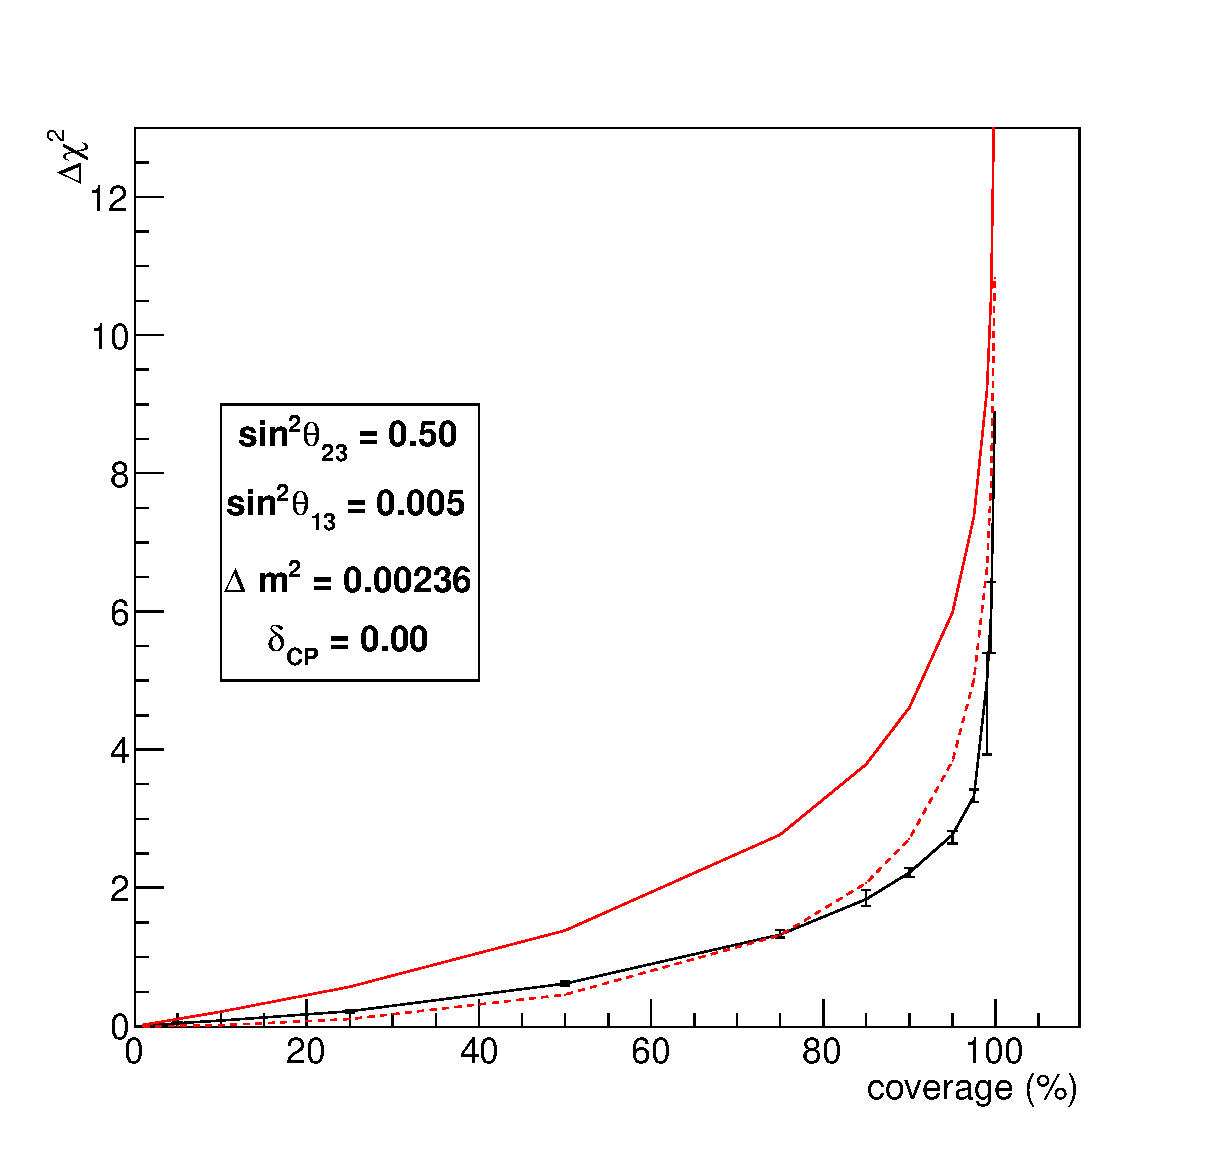
\includegraphics[width=14pc]{./images/appendix/coverage/coverage_study_2D_theta13_deltacp_syst_1.eps}
%\center
%\caption {
%   Distribution of $\Delta\chi^{2}$ vs coverage in the ($sin^{2}\theta_{13}$,$\delta_{CP}$) parameter space
%  from 1k toy MC experiments generated with the Run 1+2+3 POT
% with statistical fluctuations and systematic variations at the oscillation point: 
%  $|\Delta m^{2}| = 2.36 \times 10^{-3}$,
%  $sin^{2}\theta_{23} = 0.5$,
%  $sin^{2}\theta_{13} = 0.005$ and
%  	$\delta_{CP}$	= 0.
%	}
%\label{fig:cov_2D_theta13_deltacp_syst_1}
%\end{minipage}
%\vfill
%\vspace*{0.7cm}
%\begin{minipage}[t]{0.46\linewidth}
%\center
%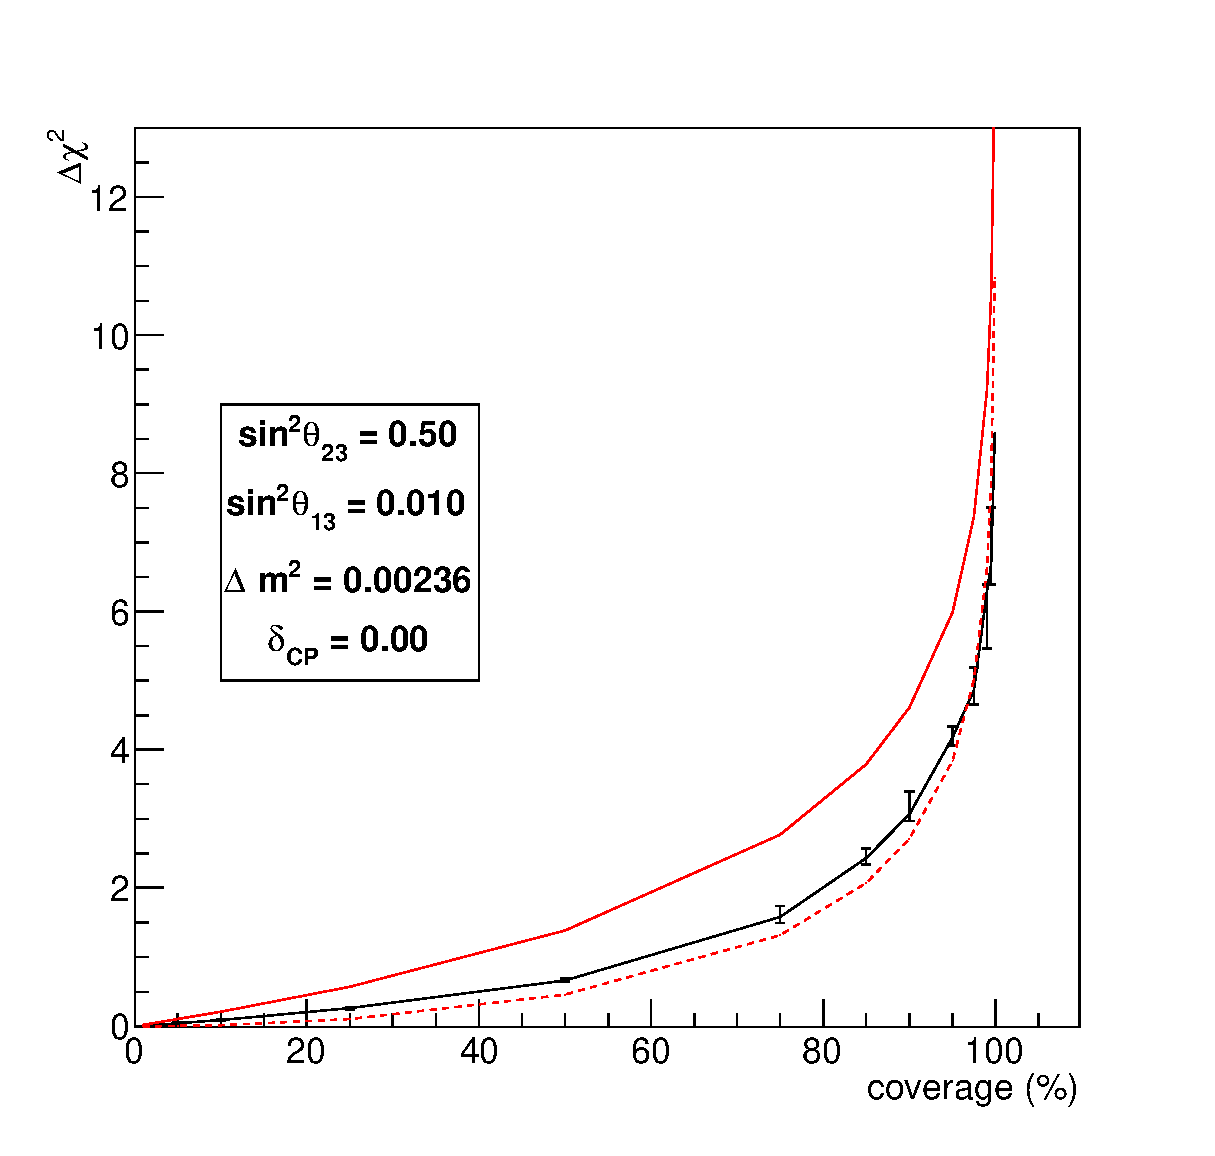
\includegraphics[width=14pc]{./images/appendix/coverage/coverage_study_2D_theta13_deltacp_syst_2.eps}
%\center
%\caption {
%   Distribution of $\Delta\chi^{2}$ vs coverage in the ($sin^{2}\theta_{13}$,$\delta_{CP}$) parameter space
%  from 1k toy MC experiments generated with the Run 1+2+3 POT
% with statistical fluctuations and systematic variations at the oscillation point: 
%  $|\Delta m^{2}| = 2.36 \times 10^{-3}$,
%  $sin^{2}\theta_{23} = 0.5$,
%  $sin^{2}\theta_{13} = 0.01$ and
%  	$\delta_{CP}$	= 0.
%	}
%\label{fig:cov_2D_theta13_deltacp_syst_2}
%\end{minipage}
%\hspace{0.03\linewidth}
%\begin{minipage}[t]{0.46\linewidth}
%\center
%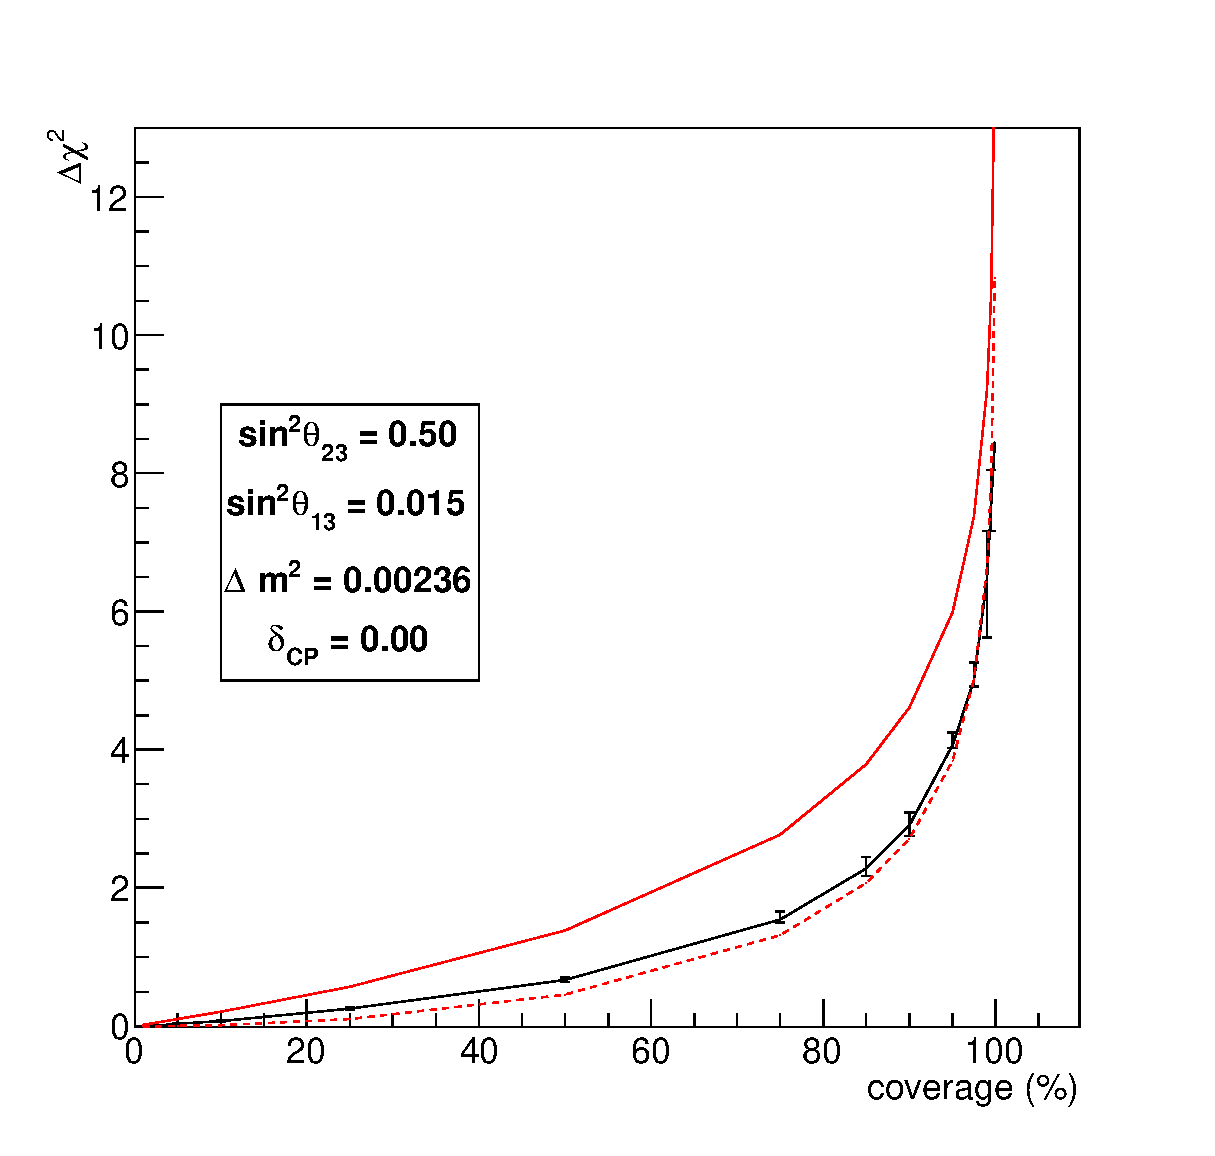
\includegraphics[width=14pc]{./images/appendix/coverage/coverage_study_2D_theta13_deltacp_syst_3.eps}
%\center
%\caption {
%   Distribution of $\Delta\chi^{2}$ vs coverage in the ($sin^{2}\theta_{13}$,$\delta_{CP}$) parameter space
%  from 1k toy MC experiments generated with the Run 1+2+3 POT
% with statistical fluctuations and systematic variations at the oscillation point: 
%  $|\Delta m^{2}| = 2.36 \times 10^{-3}$,
%  $sin^{2}\theta_{23} = 0.5$,
%  $sin^{2}\theta_{13} = 0.015$ and
%  	$\delta_{CP}$	= 0.
%	}
%\label{fig:cov_2D_theta13_deltacp_syst_3}
%\end{minipage}
%\vfill
%\vspace*{0.7cm}
%\begin{minipage}[t]{0.46\linewidth}
%\center
%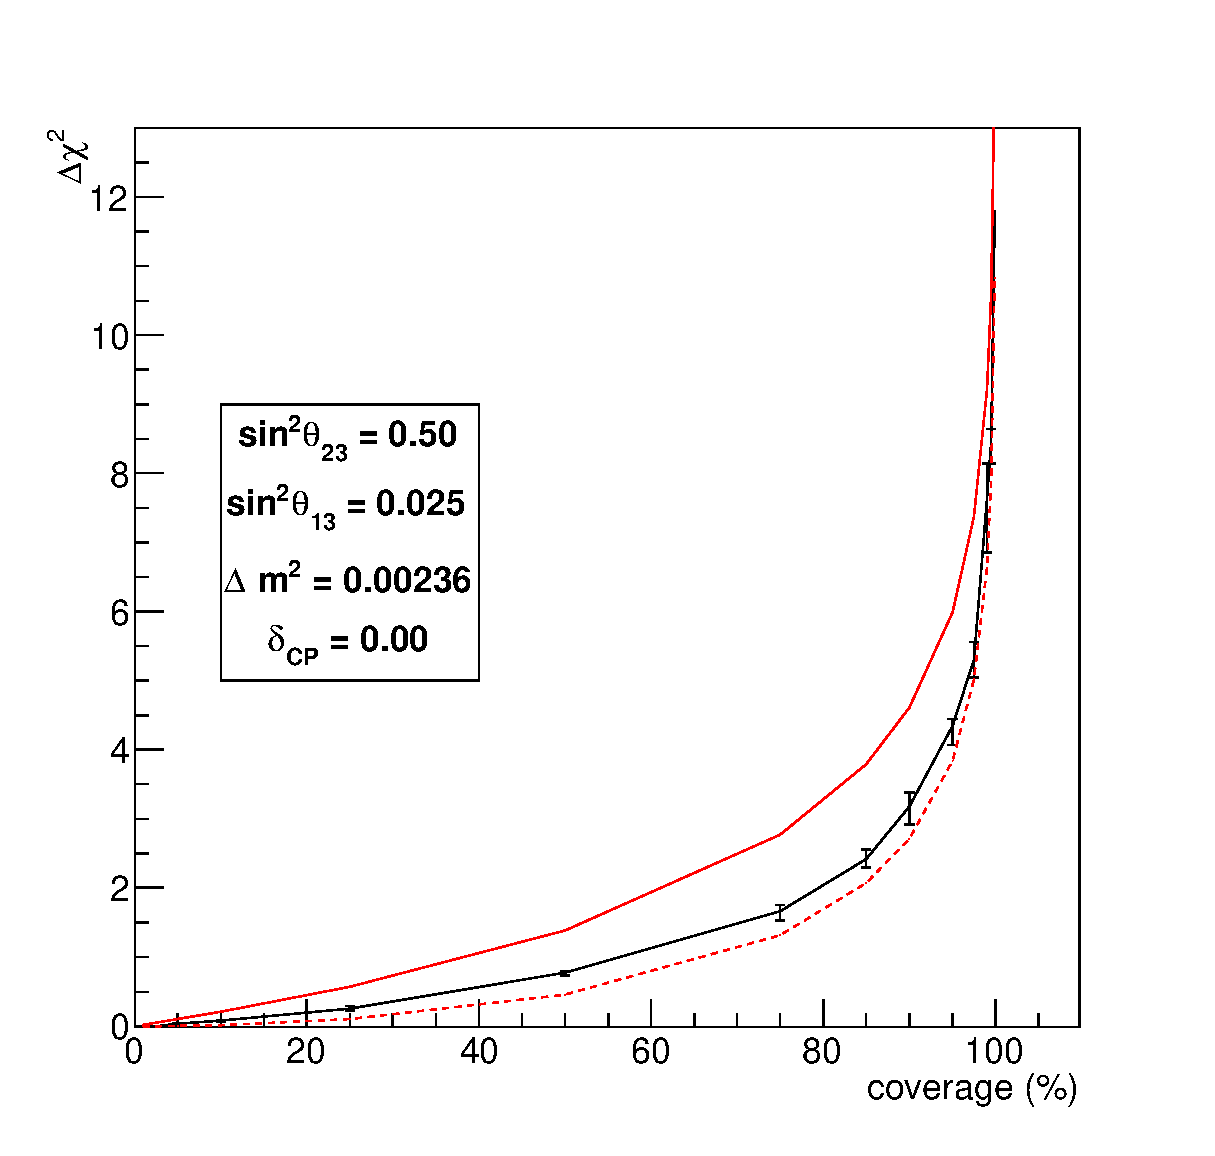
\includegraphics[width=14pc]{./images/appendix/coverage/coverage_study_2D_theta13_deltacp_syst_4.eps}
%\center
%\caption {
%   Distribution of $\Delta\chi^{2}$ vs coverage in the ($sin^{2}\theta_{13}$,$\delta_{CP}$) parameter space
%  from 1k toy MC experiments generated with the Run 1+2+3 POT
%   with statistical fluctuations and systematic variations at the oscillation point: 
%  $|\Delta m^{2}| = 2.36 \times 10^{-3}$,
%  $sin^{2}\theta_{23} = 0.5$,
%  $sin^{2}\theta_{13} = 0.025$ and
%  	$\delta_{CP}$	= 0.
%	}
%\label{fig:cov_2D_theta13_deltacp_syst_4}
%\end{minipage}
%\hspace{0.03\linewidth}




%% FIGURES FOR 2D theta13-theta23

%\begin{center}
%\begin{figure*}[htb]
%\begin{minipage}[t]{0.46\linewidth}
%\center
%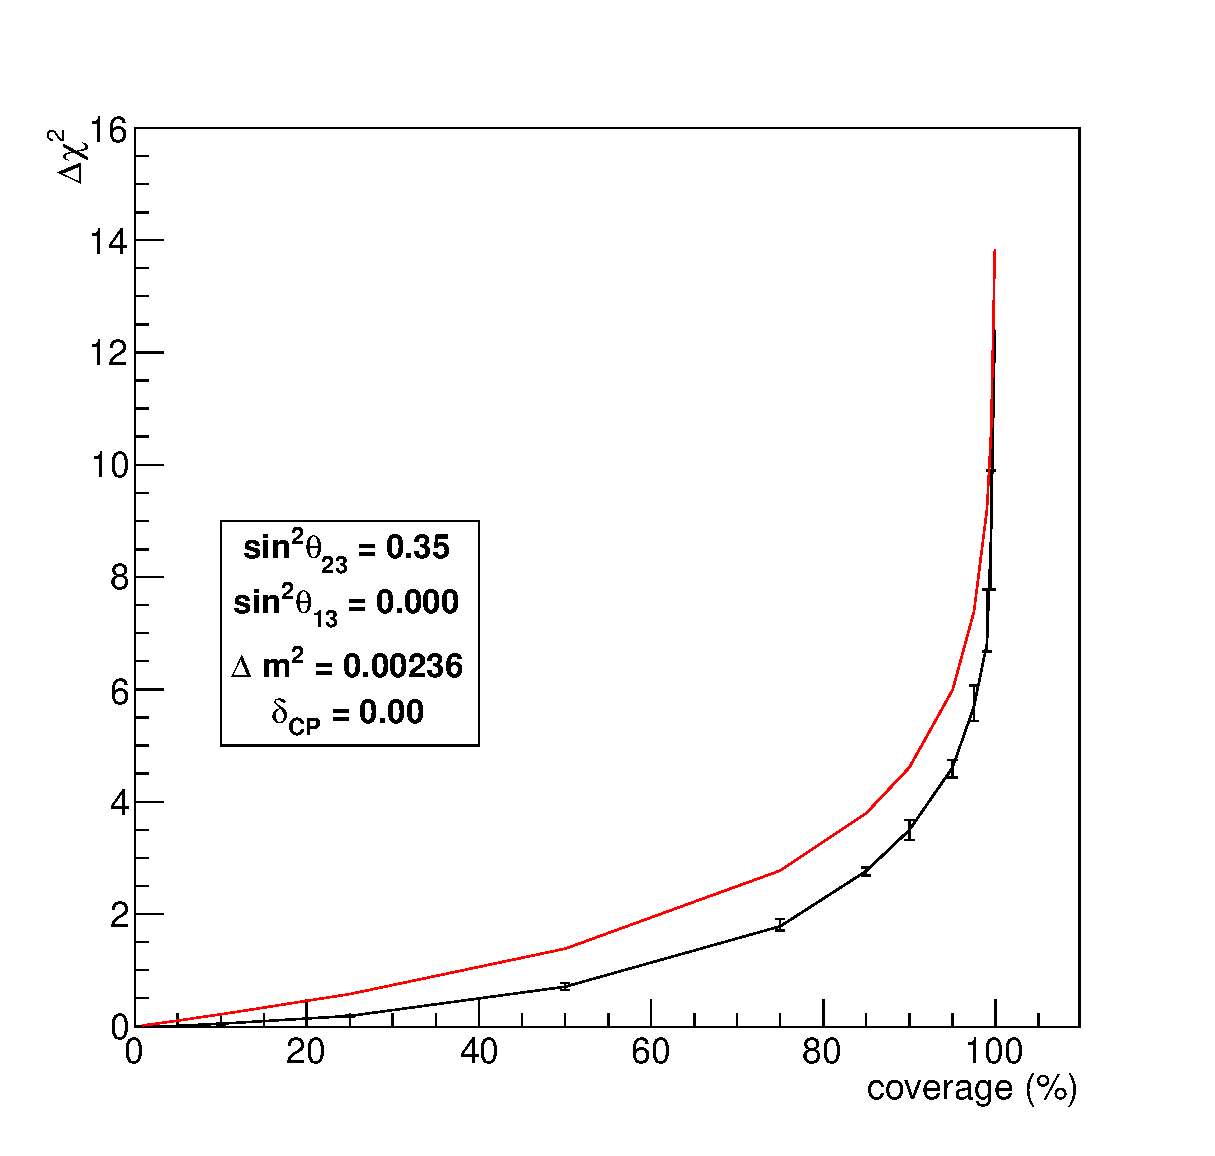
\includegraphics[width=14pc]{./images/appendix/coverage/coverage_study_2D_theta13_theta23_syst_0.eps}
%\center
%\caption {
%  Distribution of $\Delta\chi^{2}$ vs coverage in the ($sin^{2}\theta_{13}$,$sin^{2}\theta_{23}$) parameter space
%  from 1k toy MC experiments generated with the Run 1+2+3 POT
% with statistical fluctuations and systematic variations at the oscillation point indicated in the legend.
%}
%\label{fig:cov_2D_theta13_theta23_syst_0}
%\end{minipage}
%\hspace{0.03\linewidth}
%\begin{minipage}[t]{0.46\linewidth}
%\center
%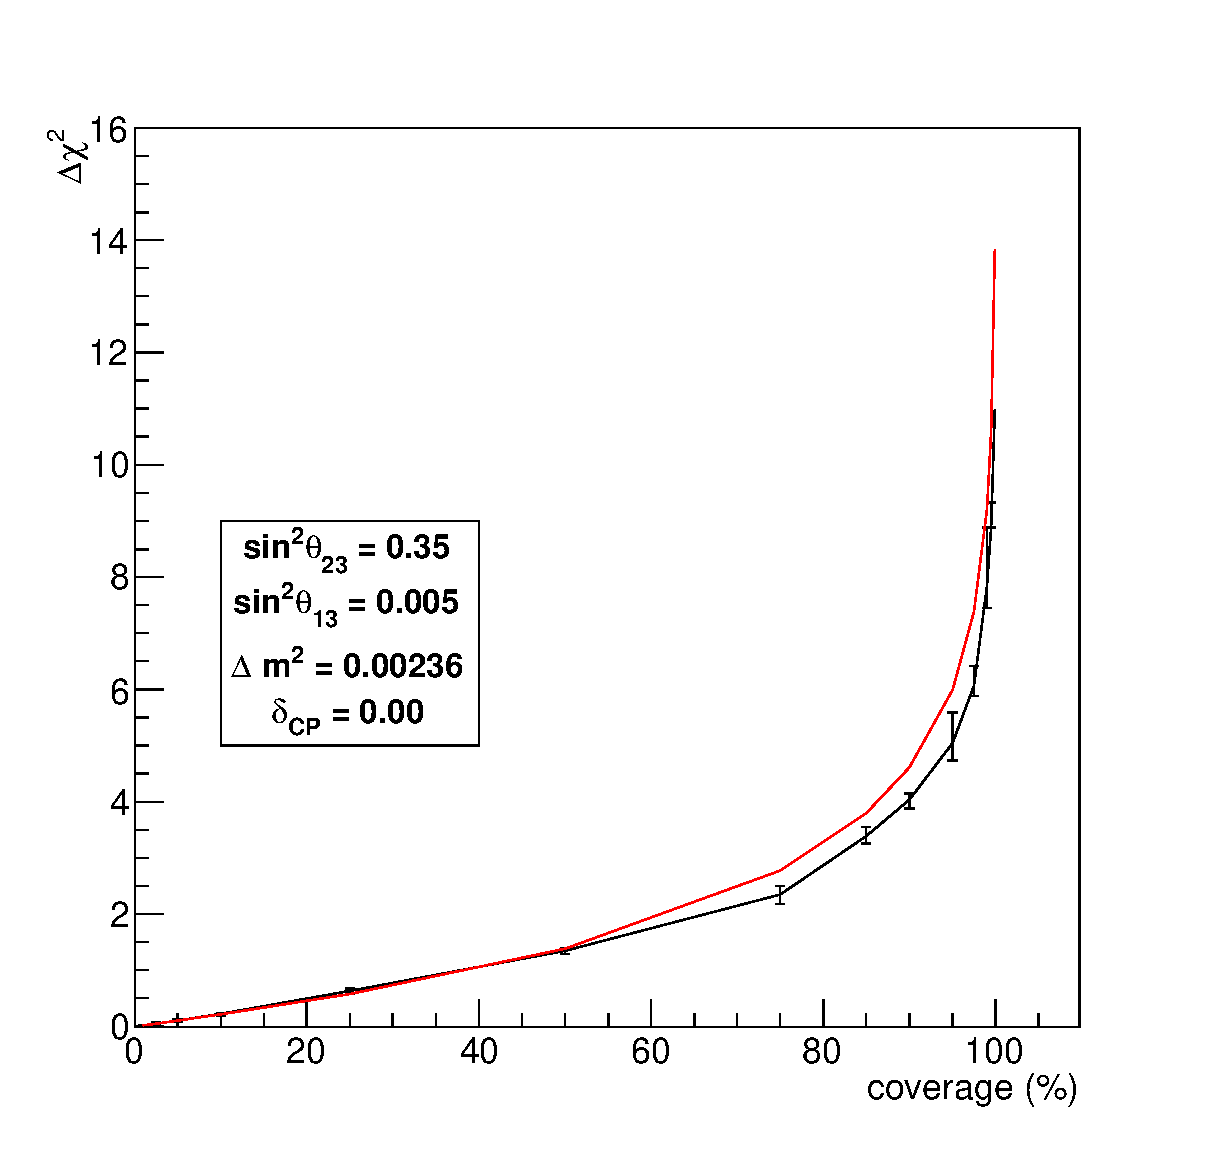
\includegraphics[width=14pc]{./images/appendix/coverage/coverage_study_2D_theta13_theta23_syst_1.eps}
%\center
%\caption {
%   Distribution of $\Delta\chi^{2}$ vs coverage in the ($sin^{2}\theta_{13}$,$sin^{2}\theta_{23}$) parameter space
%  from 1k toy MC experiments generated with the Run 1+2+3 POT
% with statistical fluctuations and systematic variations at the oscillation point indicated in the legend.
%	}
%\label{fig:cov_2D_theta13_theta23_syst_1}
%\end{minipage}
%\vfill
%\vspace*{0.7cm}
%\begin{minipage}[t]{0.46\linewidth}
%\center
%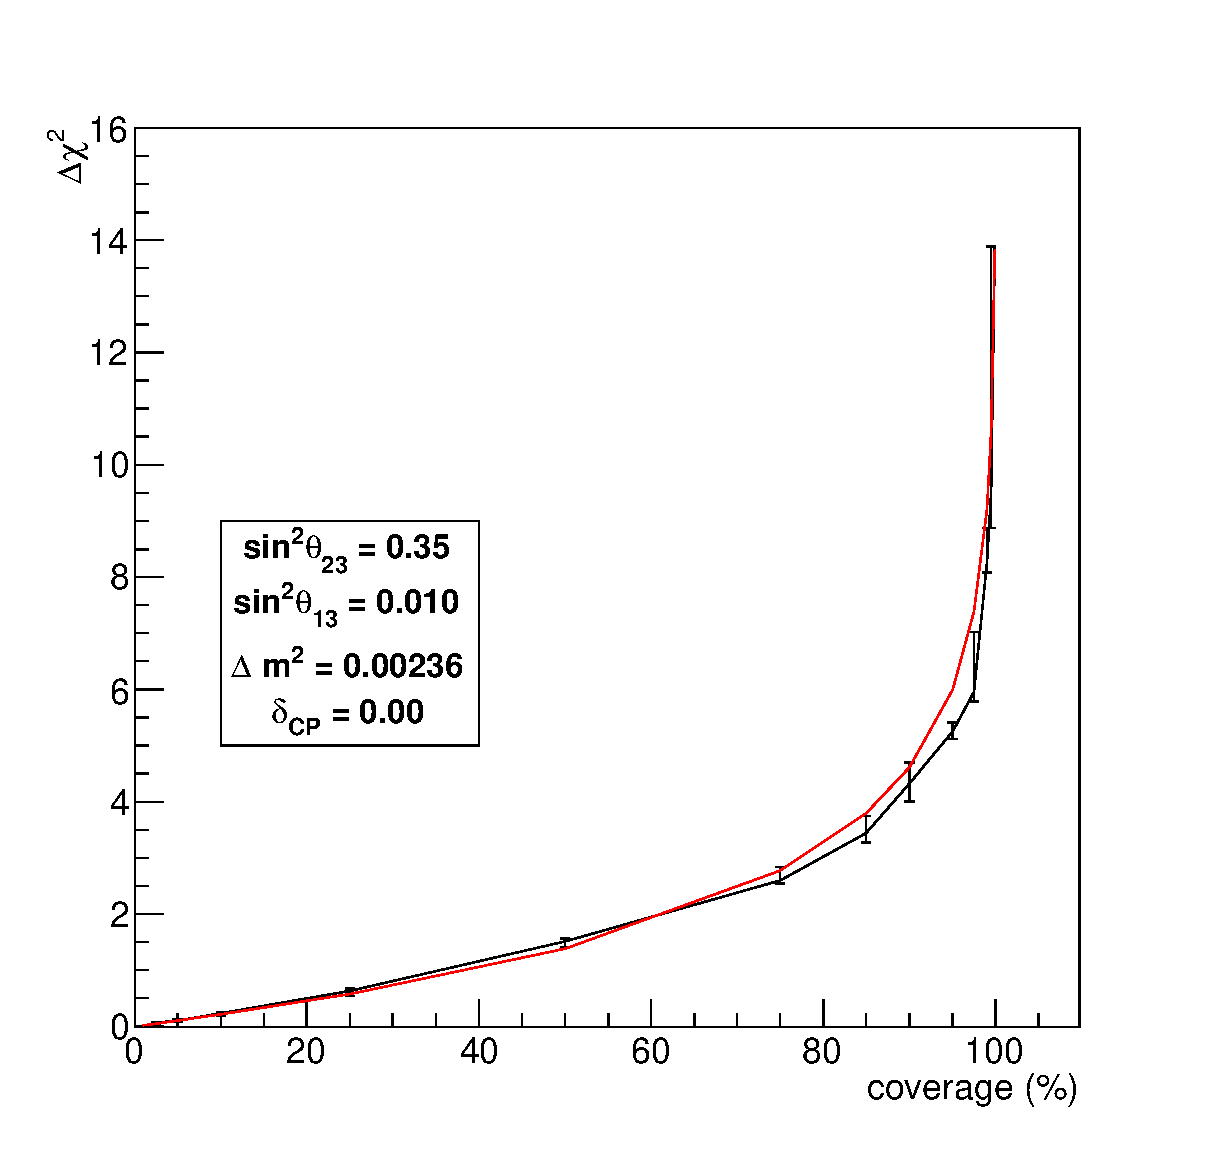
\includegraphics[width=14pc]{./images/appendix/coverage/coverage_study_2D_theta13_theta23_syst_2.eps}
%\center
%\caption {
% Distribution of $\Delta\chi^{2}$ vs coverage in the ($sin^{2}\theta_{13}$,$sin^{2}\theta_{23}$) parameter space
%  from 1k toy MC experiments generated with the Run 1+2+3 POT
% with statistical fluctuations and systematic variations at the oscillation point indicated in the legend.
%	}
%\label{fig:cov_2D_theta13_theta23_syst_2}
%\end{minipage}
%\hspace{0.03\linewidth}
%\begin{minipage}[t]{0.46\linewidth}
%\center
%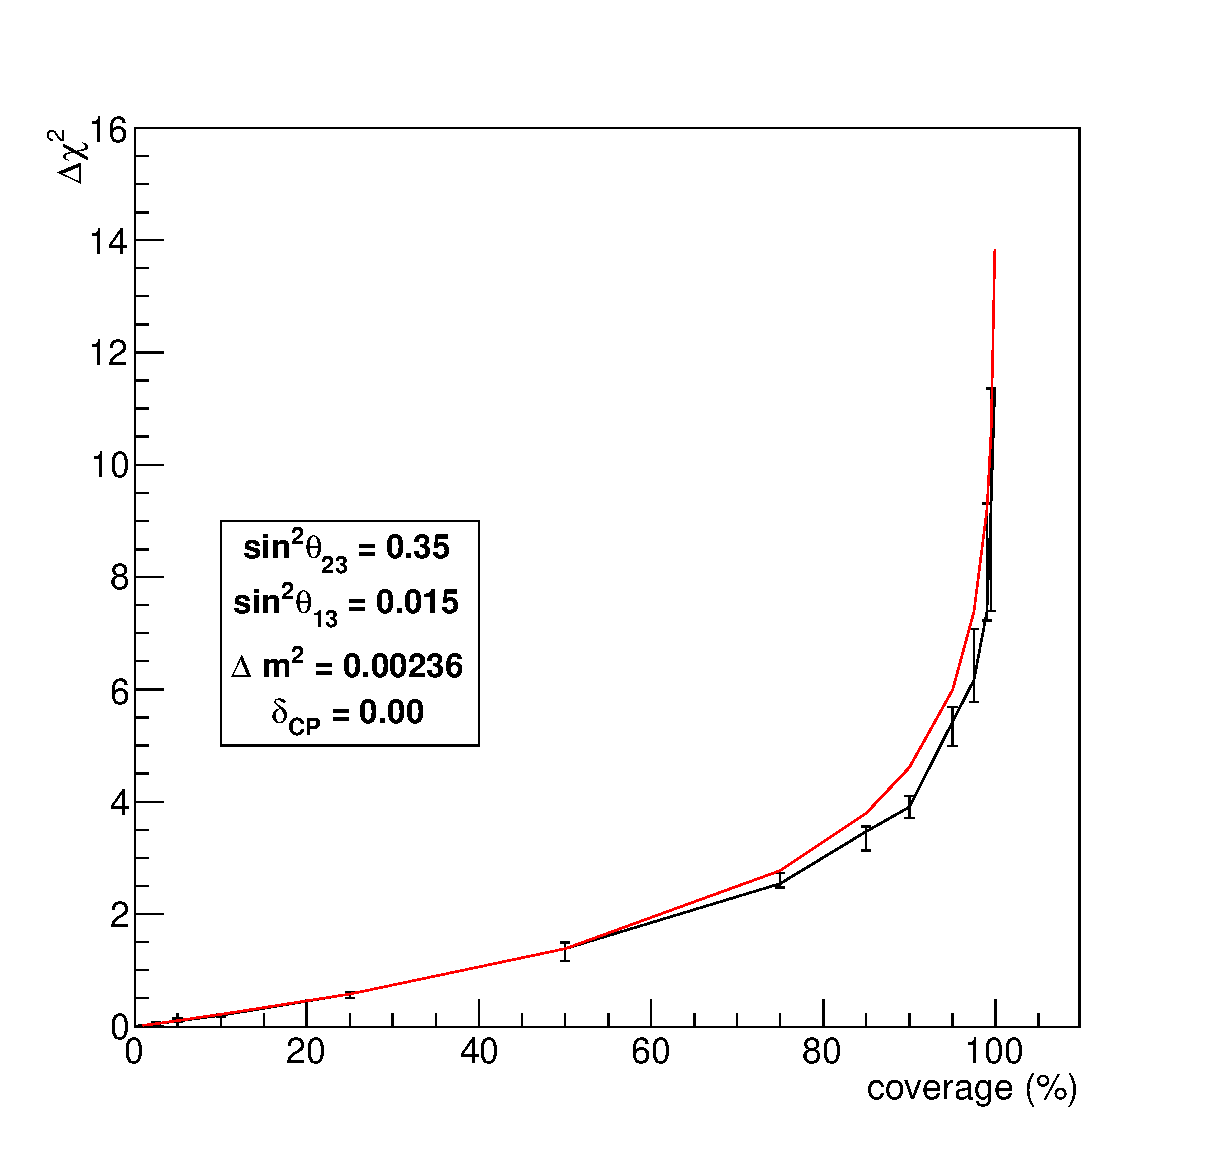
\includegraphics[width=14pc]{./images/appendix/coverage/coverage_study_2D_theta13_theta23_syst_3.eps}
%\center
%\caption {
%    Distribution of $\Delta\chi^{2}$ vs coverage in the ($sin^{2}\theta_{13}$,$sin^{2}\theta_{23}$) parameter space
%  from 1k toy MC experiments generated with the Run 1+2+3 POT
% with statistical fluctuations and systematic variations at the oscillation point indicated in the legend.
%	}
%\label{fig:cov_2D_theta13_theta23_syst_3}
%\end{minipage}
%\vfill
%\vspace*{0.7cm}
%\begin{minipage}[t]{0.46\linewidth}
%\center
%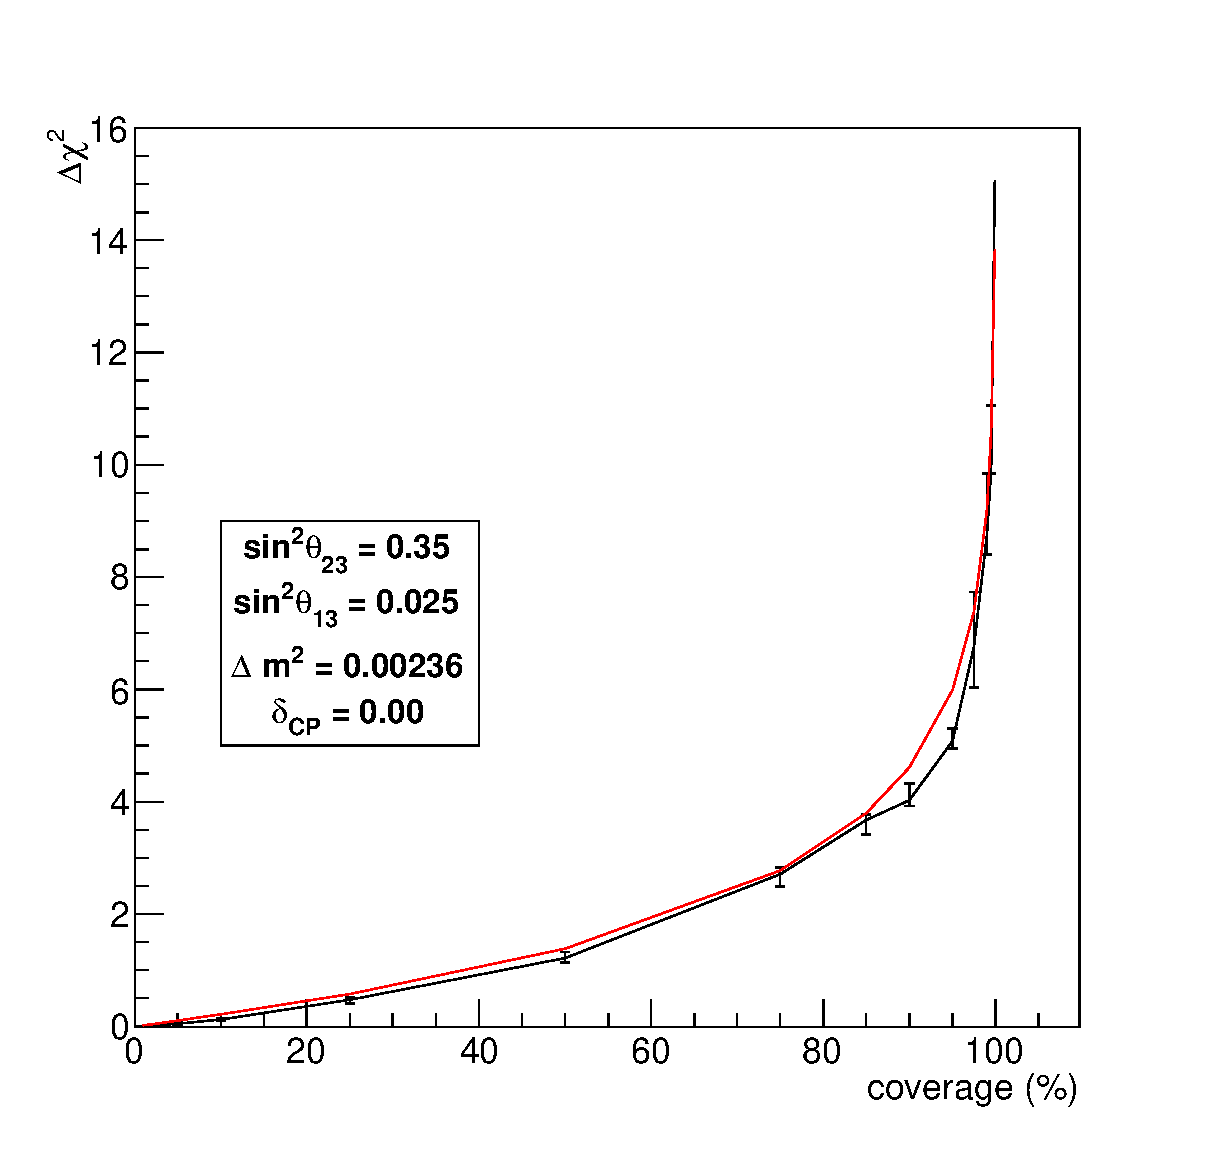
\includegraphics[width=14pc]{./images/appendix/coverage/coverage_study_2D_theta13_theta23_syst_4.eps}
%\center
%\caption {
%   Distribution of $\Delta\chi^{2}$ vs coverage in the ($sin^{2}\theta_{13}$,$sin^{2}\theta_{23}$) parameter space
%  from 1k toy MC experiments generated with the Run 1+2+3 POT
% with statistical fluctuations and systematic variations at the oscillation point indicated in the legend.
%	}
%\label{fig:cov_2D_theta13_theta23_syst_4}
%\end{minipage}
%\hspace{0.03\linewidth}
%\begin{minipage}[t]{0.46\linewidth}
%\center
%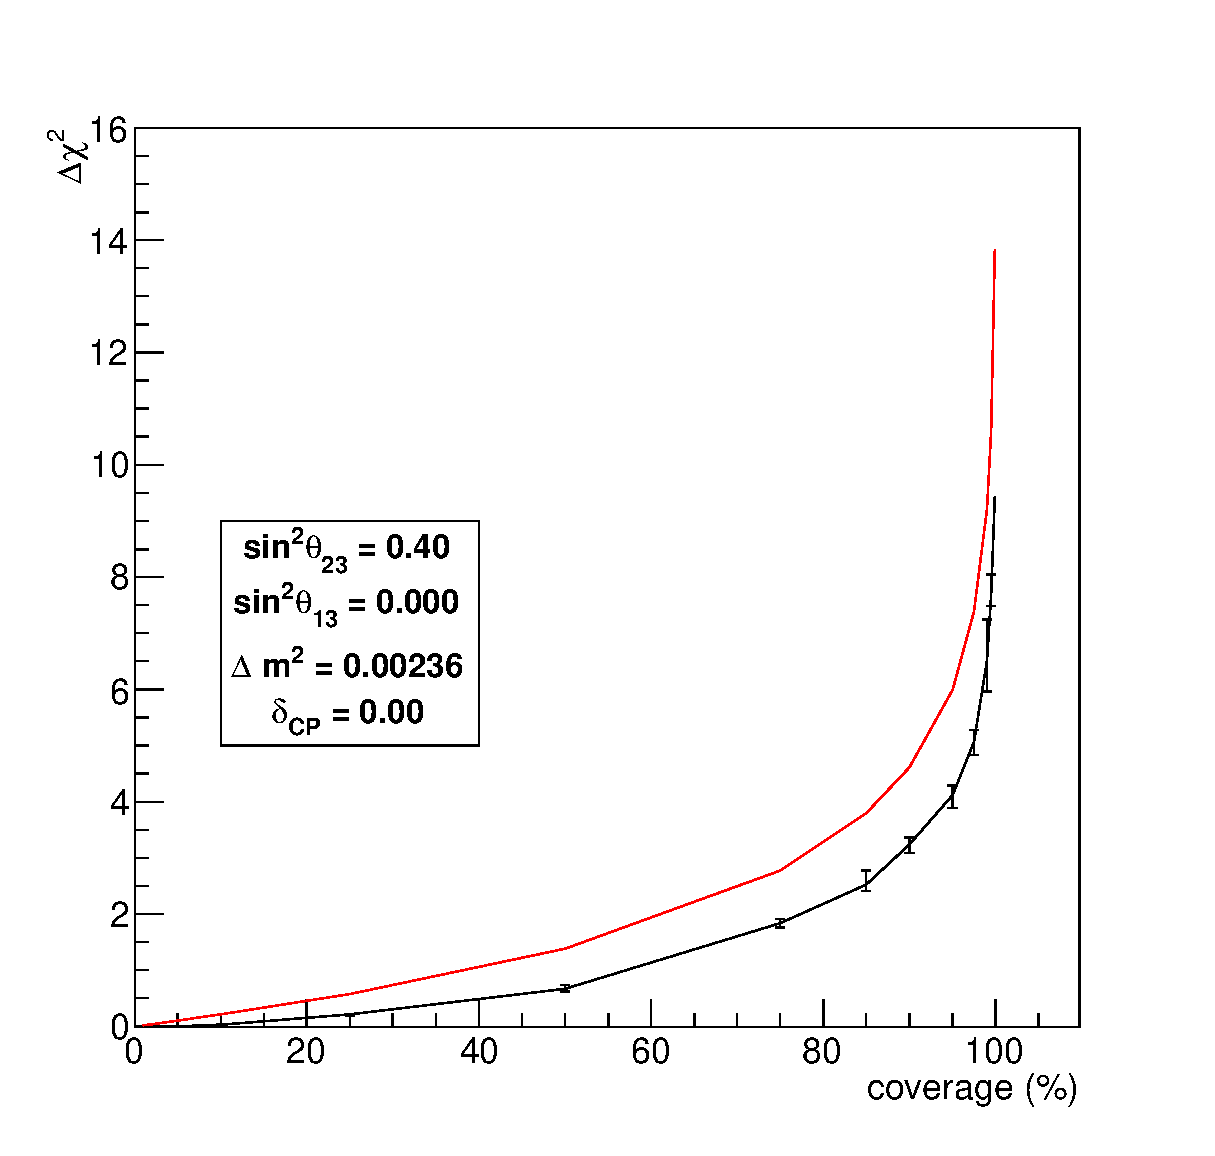
\includegraphics[width=14pc]{./images/appendix/coverage/coverage_study_2D_theta13_theta23_syst_5.eps}
%\center
%\caption {
%    Distribution of $\Delta\chi^{2}$ vs coverage in the ($sin^{2}\theta_{13}$,$sin^{2}\theta_{23}$) parameter space
%  from 1k toy MC experiments generated with the Run 1+2+3 POT
% with statistical fluctuations and systematic variations at the oscillation point indicated in the legend.
%		}
%\label{fig:cov_2D_theta13_theta23_syst_5}
%\end{minipage}
%\end{figure*}
%\end{center}



%\begin{center}
%\begin{figure*}[htb]
%\begin{minipage}[t]{0.46\linewidth}
%\center
%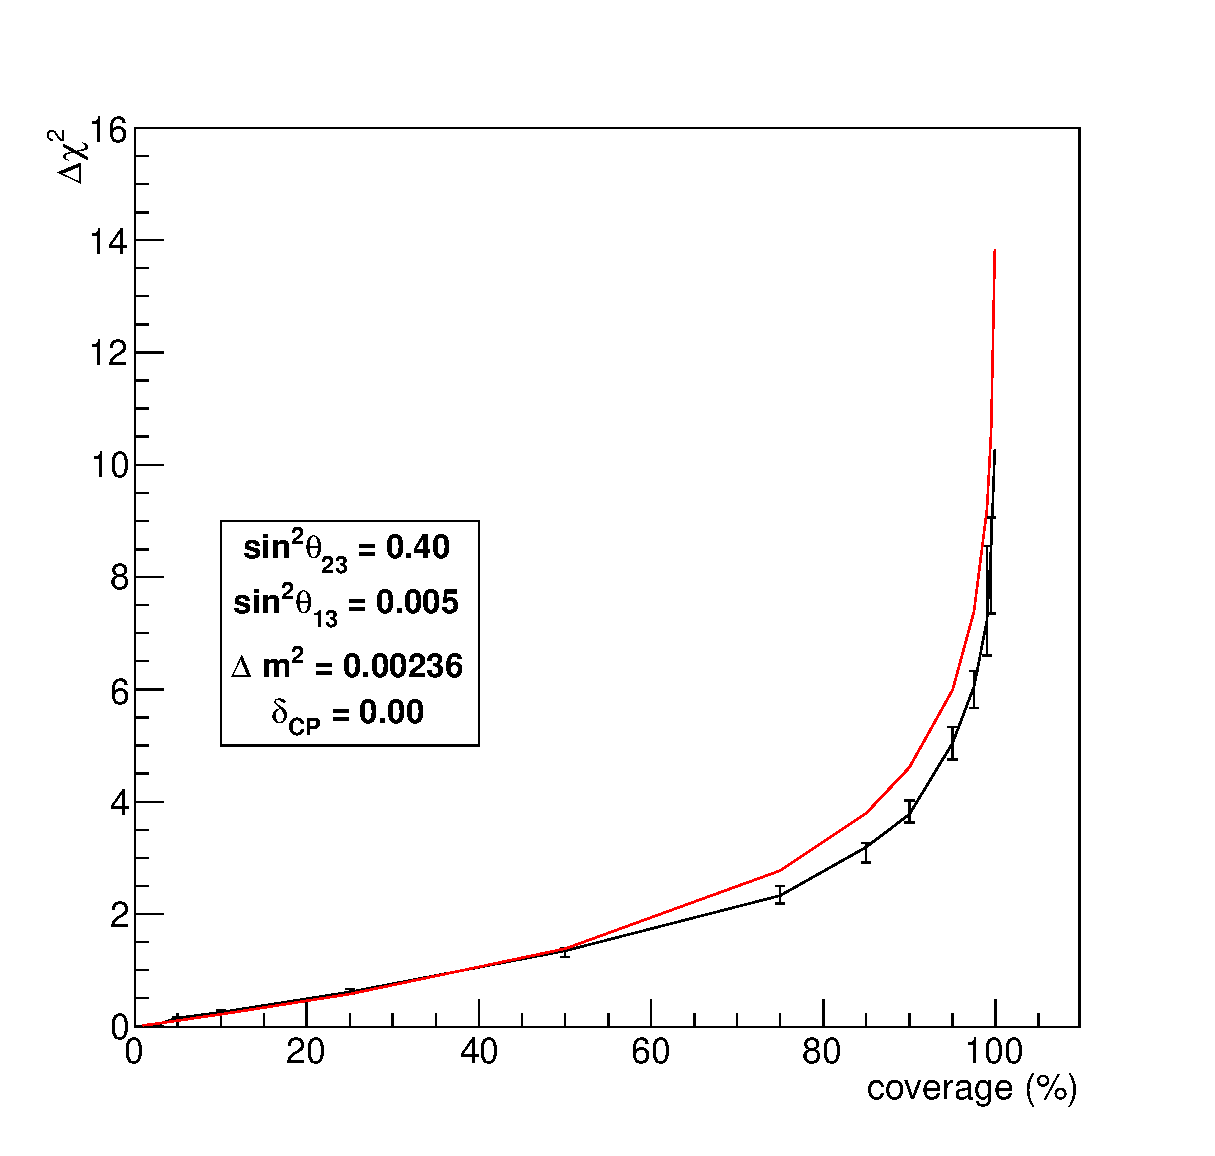
\includegraphics[width=14pc]{./images/appendix/coverage/coverage_study_2D_theta13_theta23_syst_6.eps}
%\center
%\caption {
%  Distribution of $\Delta\chi^{2}$ vs coverage in the ($sin^{2}\theta_{13}$,$sin^{2}\theta_{23}$) parameter space
%  from 1k toy MC experiments generated with the Run 1+2+3 POT
% with statistical fluctuations and systematic variations at the oscillation point indicated in the legend.
%}
%\label{fig:cov_2D_theta13_theta23_syst_6}
%\end{minipage}
%\hspace{0.03\linewidth}
%\begin{minipage}[t]{0.46\linewidth}
%\center
%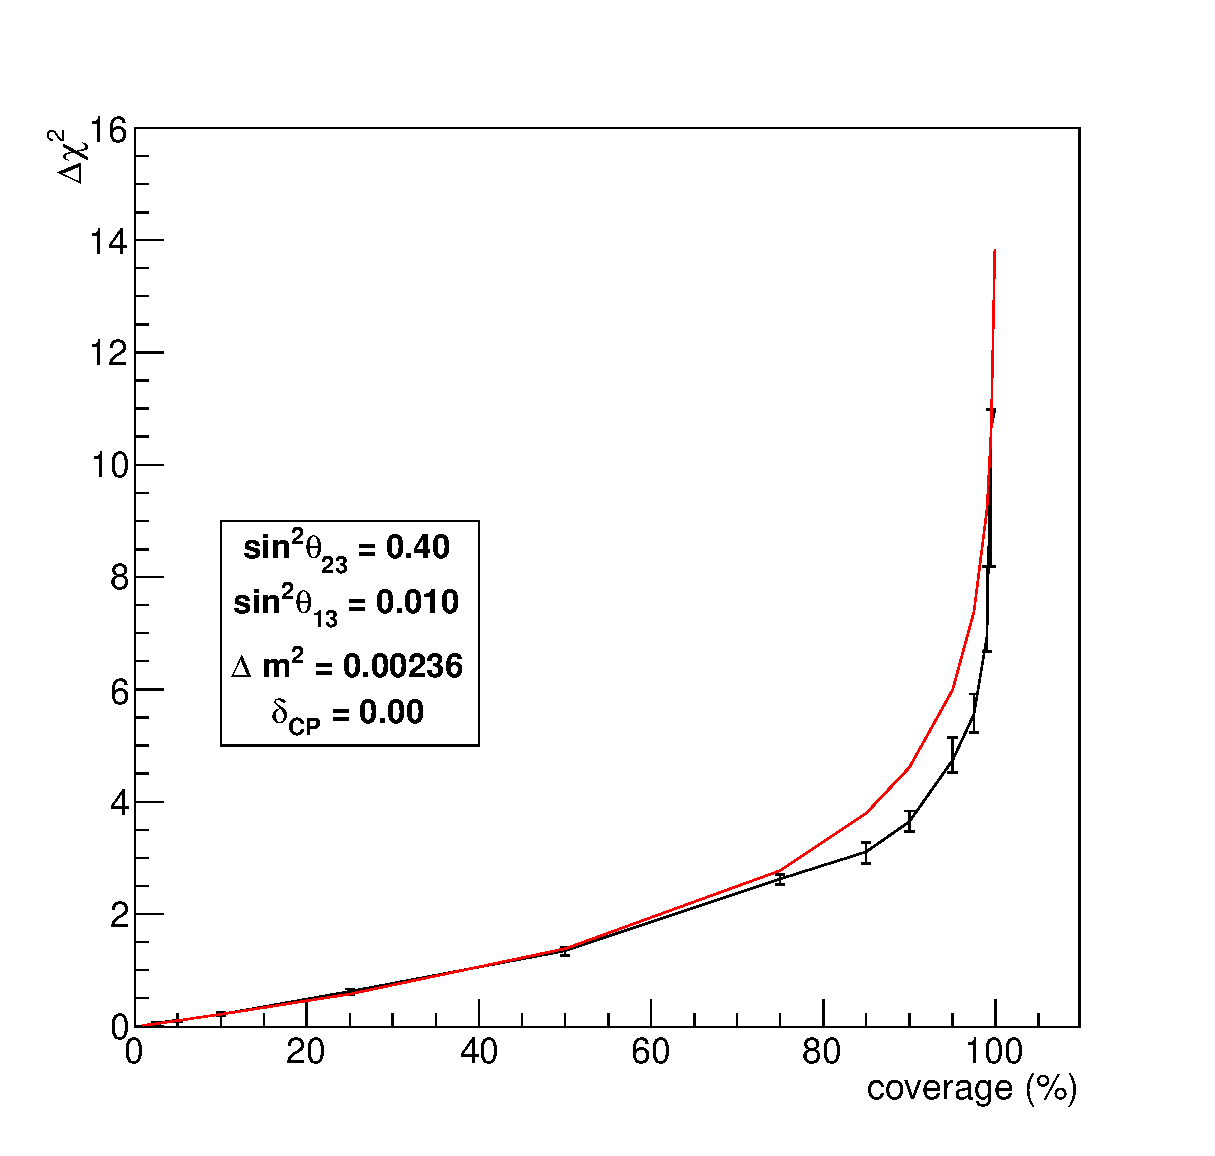
\includegraphics[width=14pc]{./images/appendix/coverage/coverage_study_2D_theta13_theta23_syst_7.eps}
%\center
%\caption {
%    Distribution of $\Delta\chi^{2}$ vs coverage in the ($sin^{2}\theta_{13}$,$sin^{2}\theta_{23}$) parameter space
%  from 1k toy MC experiments generated with the Run 1+2+3 POT
% with statistical fluctuations and systematic variations at the oscillation point indicated in the legend.
%	}
%\label{fig:cov_2D_theta13_theta23_syst_7}
%\end{minipage}
%\vfill
%\vspace*{0.7cm}
%\begin{minipage}[t]{0.46\linewidth}
%\center
%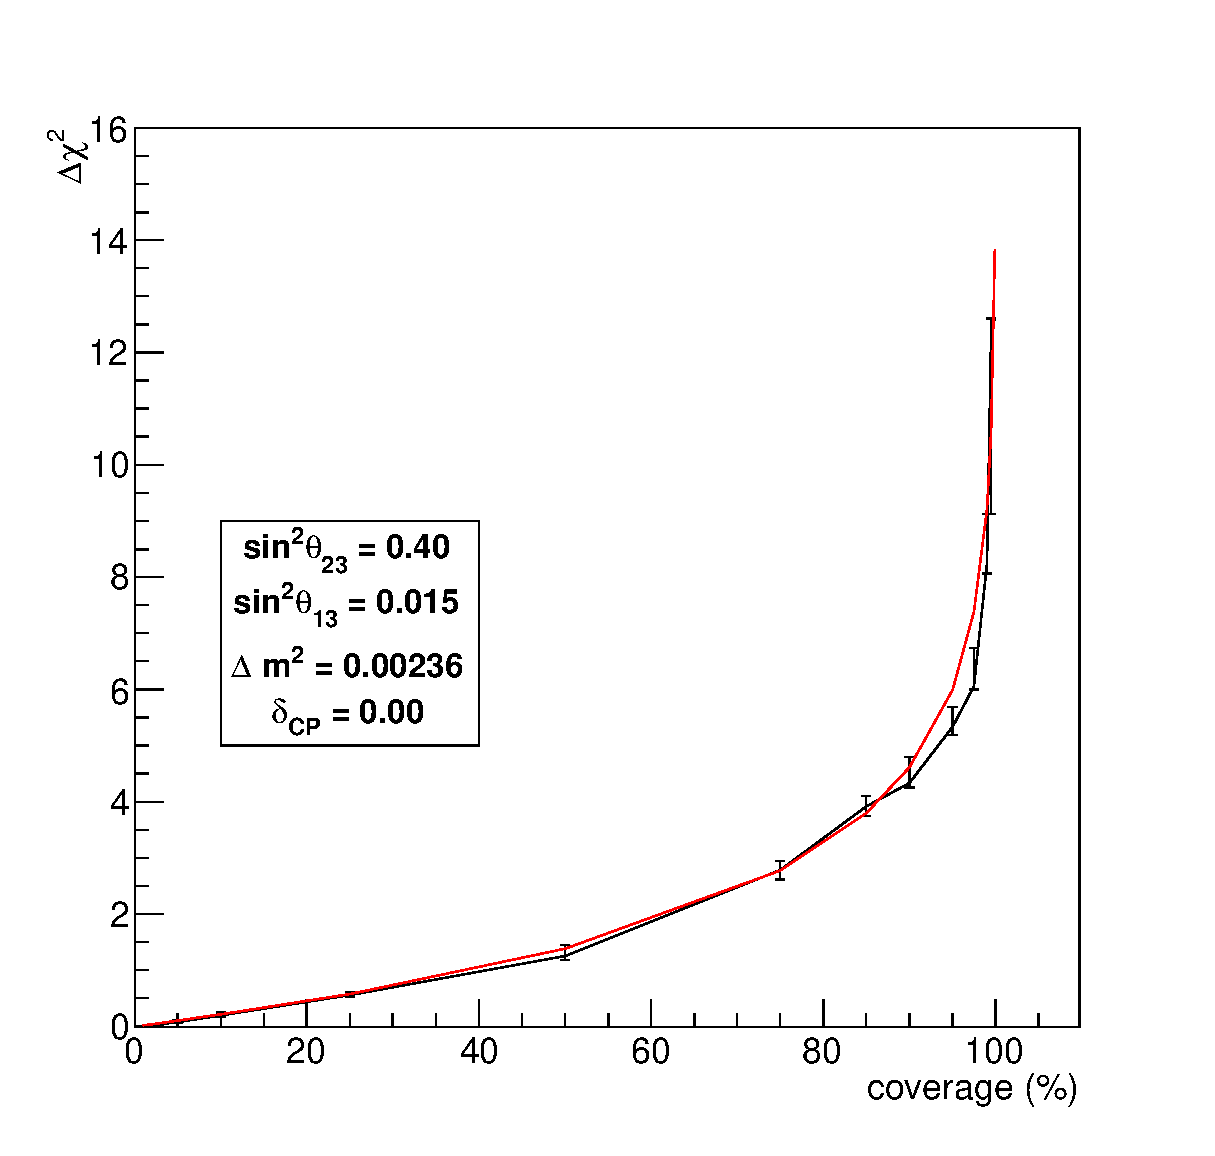
\includegraphics[width=14pc]{./images/appendix/coverage/coverage_study_2D_theta13_theta23_syst_8.eps}
%\center
%\caption {
%   Distribution of $\Delta\chi^{2}$ vs coverage in the ($sin^{2}\theta_{13}$,$sin^{2}\theta_{23}$) parameter space
%  from 1k toy MC experiments generated with the Run 1+2+3 POT
% with statistical fluctuations and systematic variations at the oscillation point indicated in the legend.
%	}
%\label{fig:cov_2D_theta13_theta23_syst_8}
%\end{minipage}
%\hspace{0.03\linewidth}
%\begin{minipage}[t]{0.46\linewidth}
%\center
%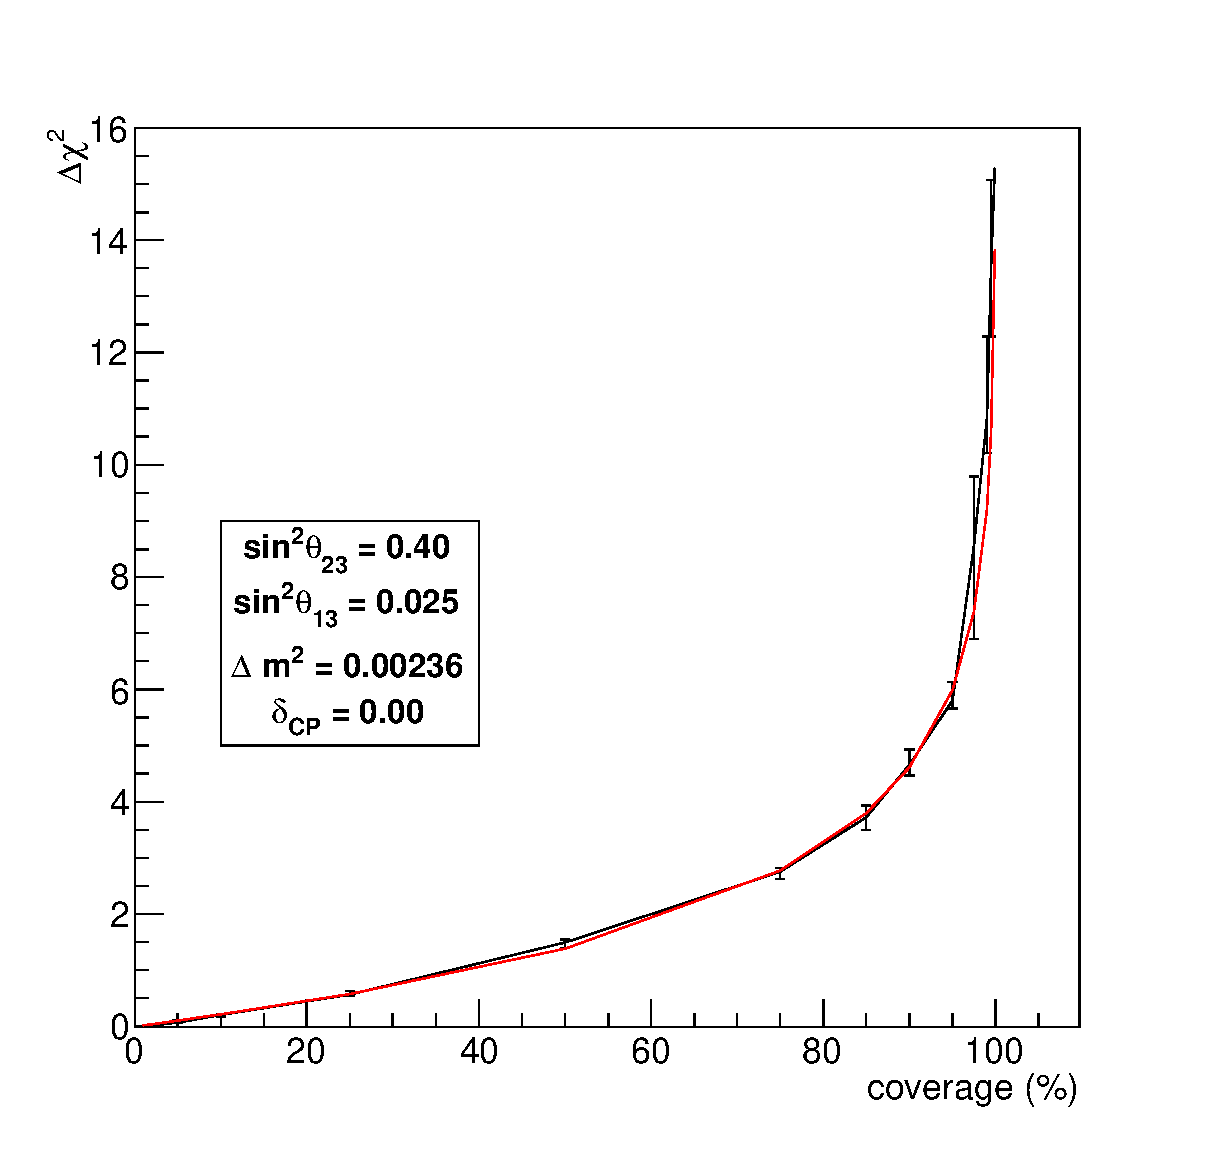
\includegraphics[width=14pc]{./images/appendix/coverage/coverage_study_2D_theta13_theta23_syst_9.eps}
%\center
%\caption {
%    Distribution of $\Delta\chi^{2}$ vs coverage in the ($sin^{2}\theta_{13}$,$sin^{2}\theta_{23}$) parameter space
%  from 1k toy MC experiments generated with the Run 1+2+3 POT
% with statistical fluctuations and systematic variations at the oscillation point indicated in the legend.
%	}
%\label{fig:cov_2D_theta13_theta23_syst_9}
%\end{minipage}
%\vfill
%\vspace*{0.7cm}
%\begin{minipage}[t]{0.46\linewidth}
%\center
%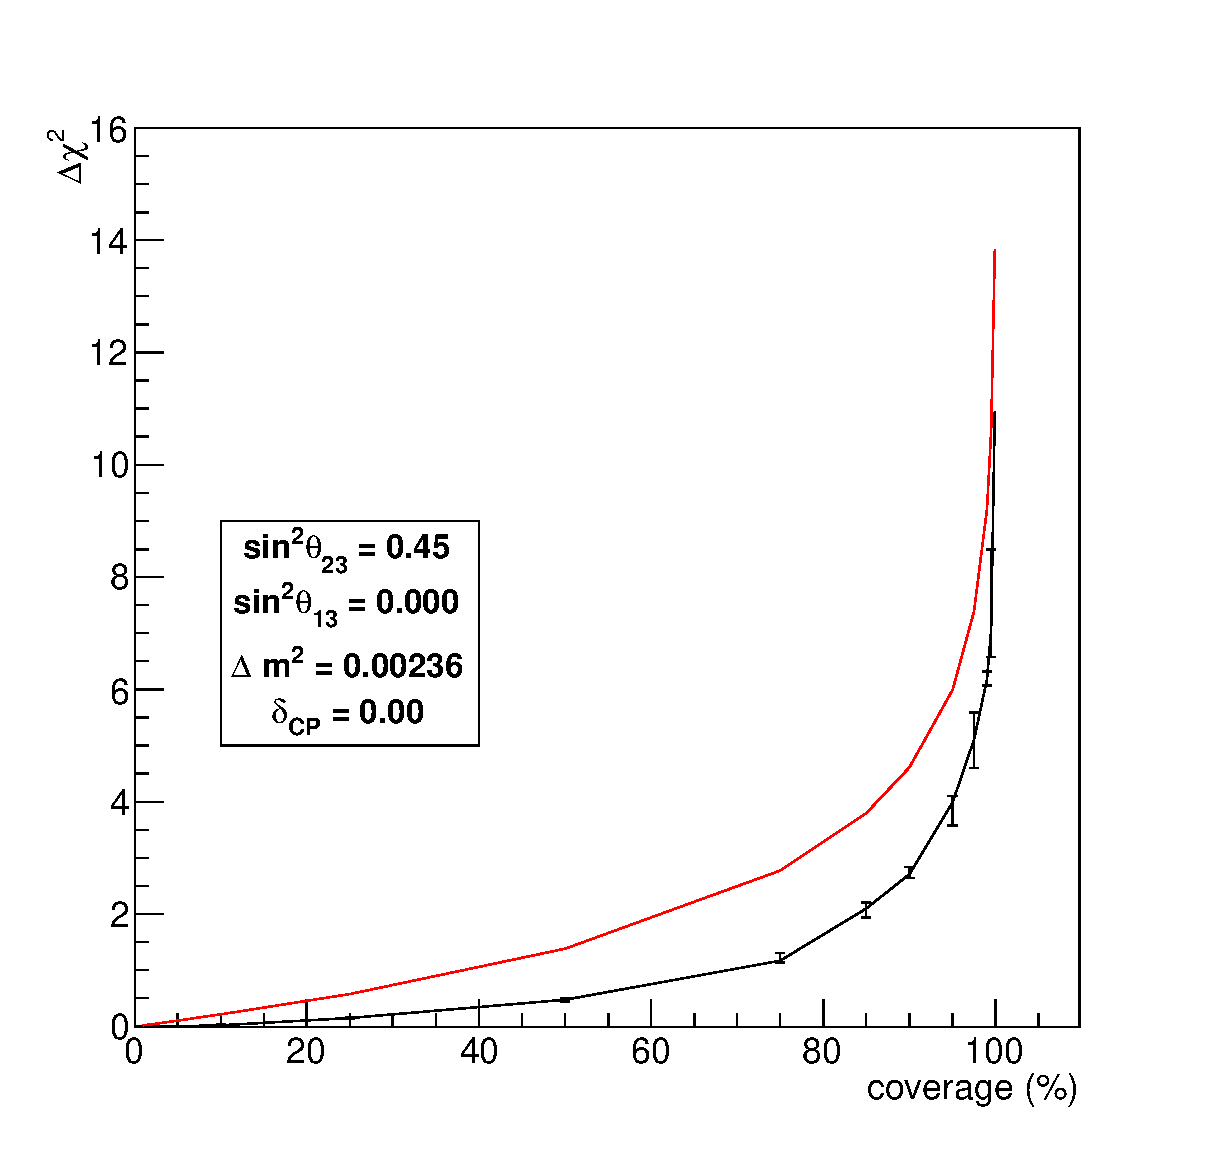
\includegraphics[width=14pc]{./images/appendix/coverage/coverage_study_2D_theta13_theta23_syst_10.eps}
%\center
%\caption {
%    Distribution of $\Delta\chi^{2}$ vs coverage in the ($sin^{2}\theta_{13}$,$sin^{2}\theta_{23}$) parameter space
%  from 1k toy MC experiments generated with the Run 1+2+3 POT
% with statistical fluctuations and systematic variations at the oscillation point indicated in the legend.
%	}
%\label{fig:cov_2D_theta13_theta23_syst_10}
%\end{minipage}
%\hspace{0.03\linewidth}
%\begin{minipage}[t]{0.46\linewidth}
%\center
%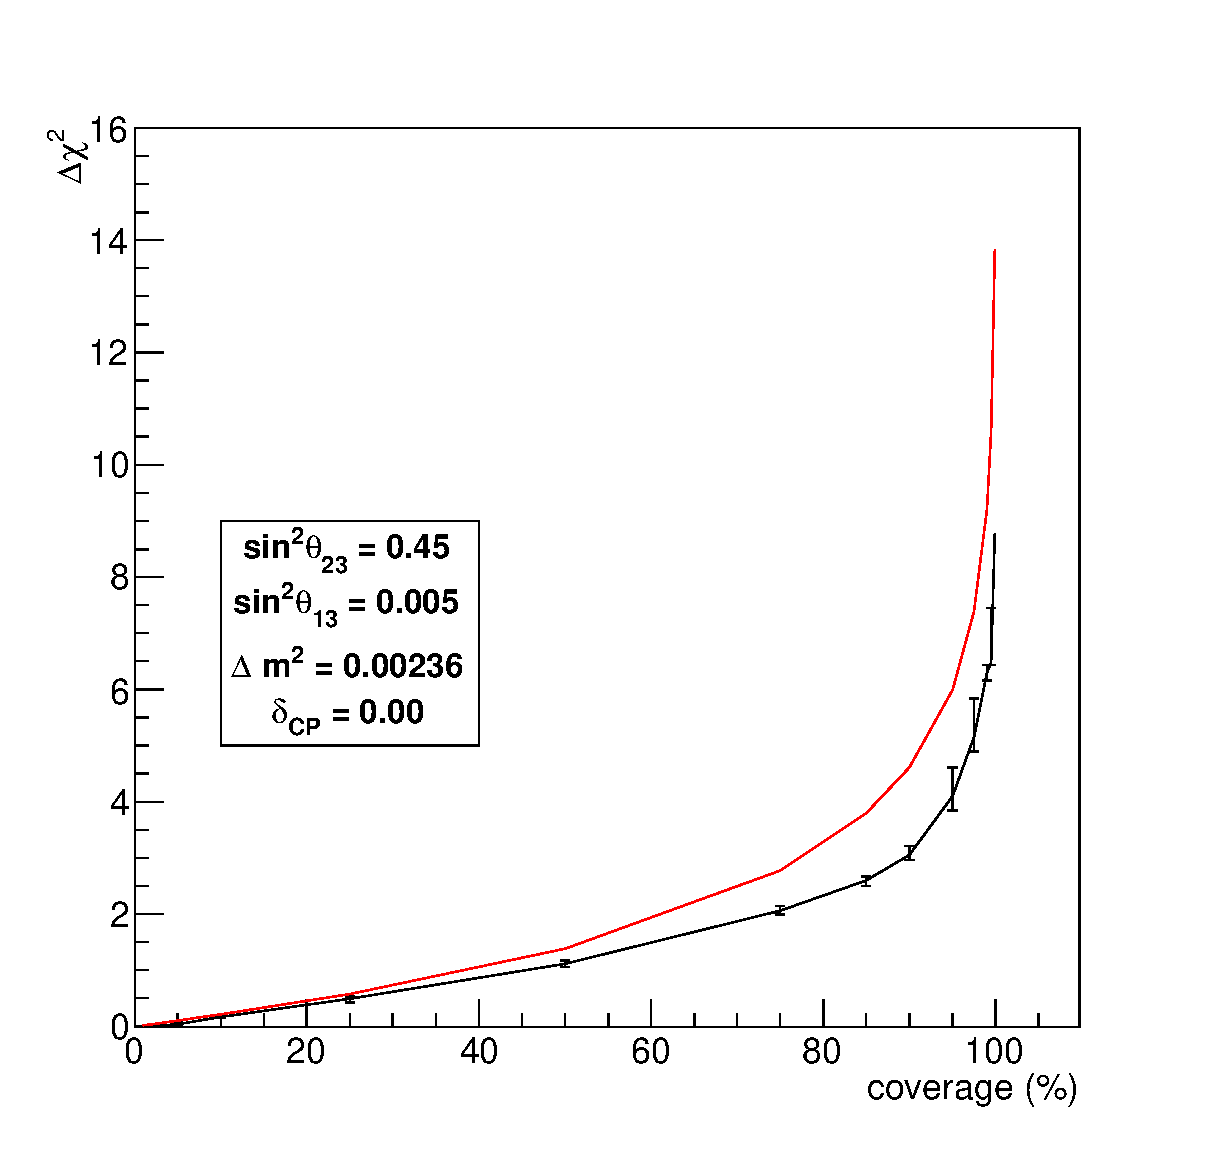
\includegraphics[width=14pc]{./images/appendix/coverage/coverage_study_2D_theta13_theta23_syst_11.eps}
%\center
%\caption {
%     Distribution of $\Delta\chi^{2}$ vs coverage in the ($sin^{2}\theta_{13}$,$sin^{2}\theta_{23}$) parameter space
%  from 1k toy MC experiments generated with the Run 1+2+3 POT
% with statistical fluctuations and systematic variations at the oscillation point indicated in the legend.
%		}
%\label{fig:cov_2D_theta13_theta23_syst_11}
%\end{minipage}
%\end{figure*}
%\end{center}



%\begin{center}
%\begin{figure*}[htb]
%\begin{minipage}[t]{0.46\linewidth}
%\center
%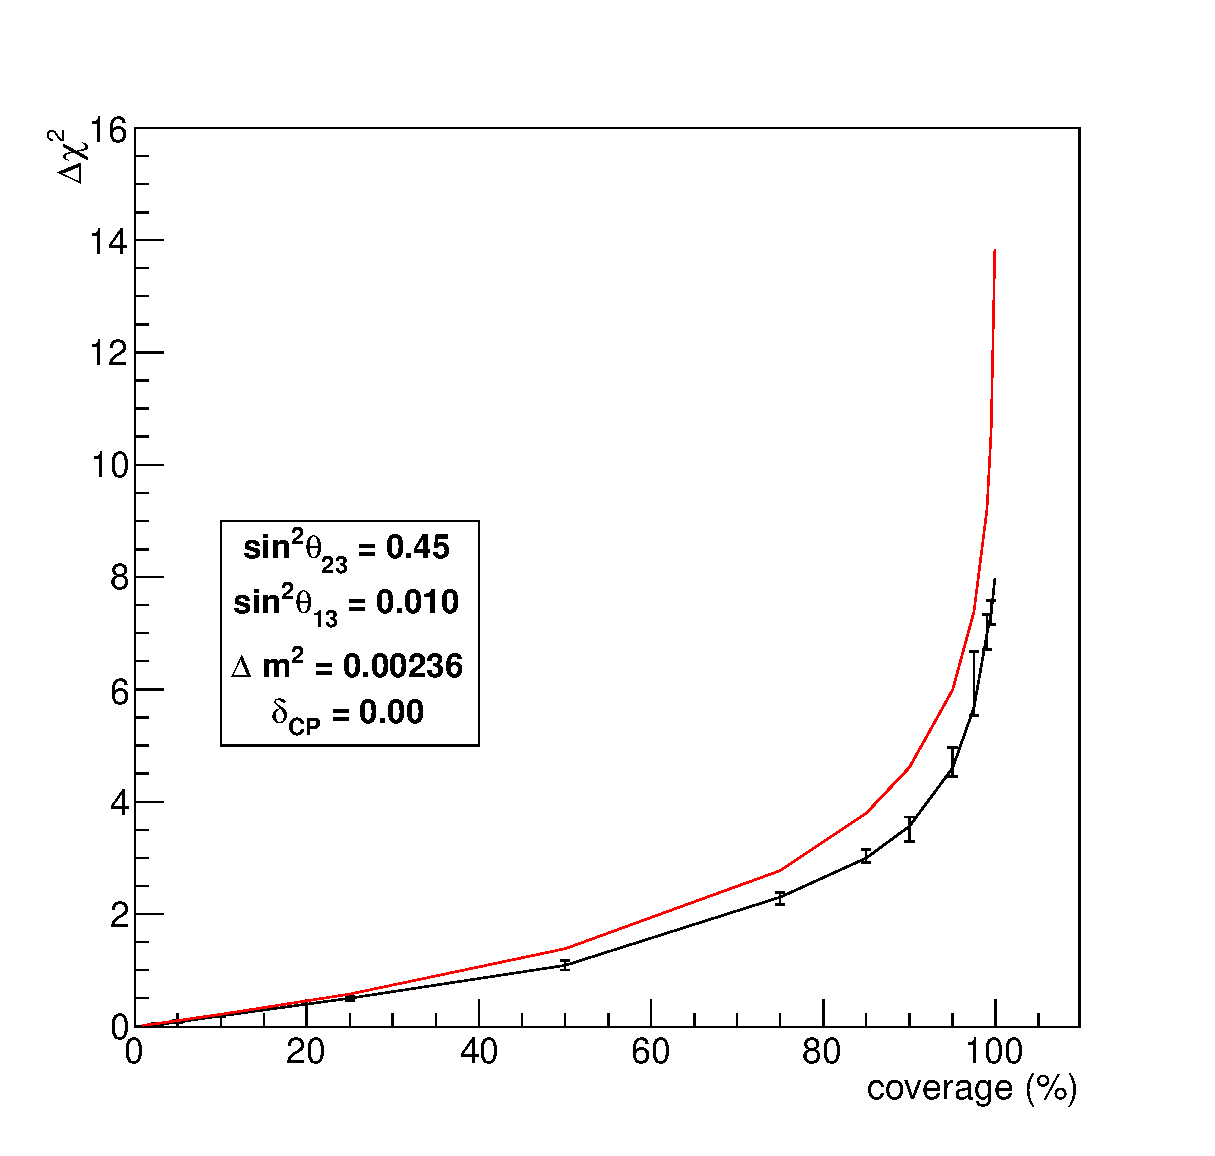
\includegraphics[width=14pc]{./images/appendix/coverage/coverage_study_2D_theta13_theta23_syst_12.eps}
%\center
%\caption {
%   Distribution of $\Delta\chi^{2}$ vs coverage in the ($sin^{2}\theta_{13}$,$sin^{2}\theta_{23}$) parameter space
%  from 1k toy MC experiments generated with the Run 1+2+3 POT
% with statistical fluctuations and systematic variations at the oscillation point indicated in the legend.
%}
%\label{fig:cov_2D_theta13_theta23_syst_12}
%\end{minipage}
%\hspace{0.03\linewidth}
%\begin{minipage}[t]{0.46\linewidth}
%\center
%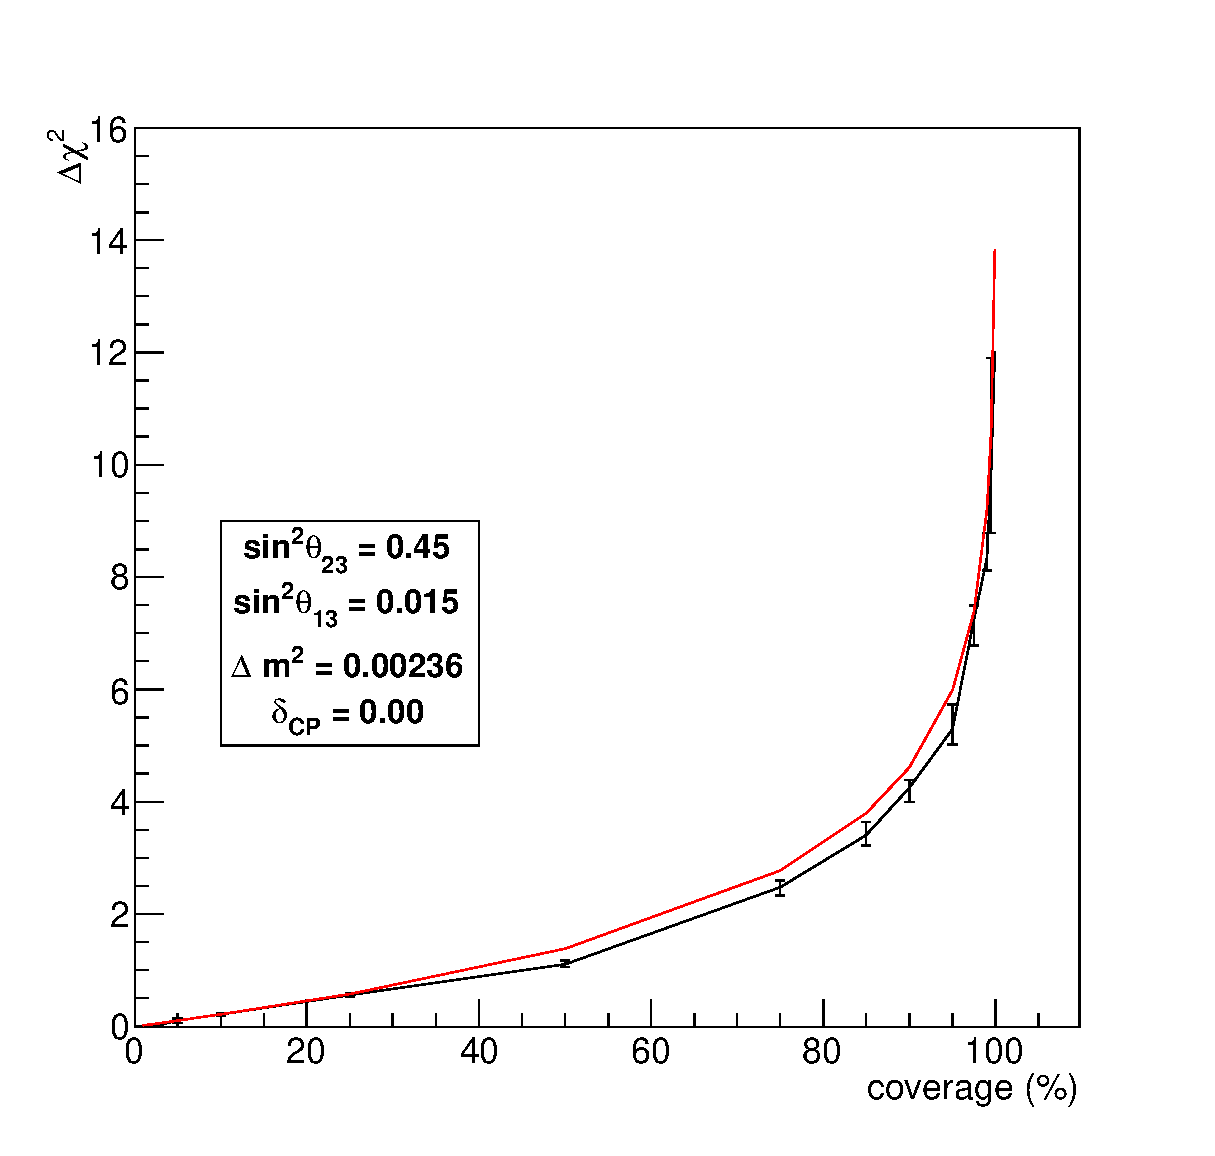
\includegraphics[width=14pc]{./images/appendix/coverage/coverage_study_2D_theta13_theta23_syst_13.eps}
%\center
%\caption {
% Distribution of $\Delta\chi^{2}$ vs coverage in the ($sin^{2}\theta_{13}$,$sin^{2}\theta_{23}$) parameter space
%  from 1k toy MC experiments generated with the Run 1+2+3 POT
% with statistical fluctuations and systematic variations at the oscillation point indicated in the legend.
%	}
%\label{fig:cov_2D_theta13_theta23_syst_13}
%\end{minipage}
%\vfill
%\vspace*{0.7cm}
%\begin{minipage}[t]{0.46\linewidth}
%\center
%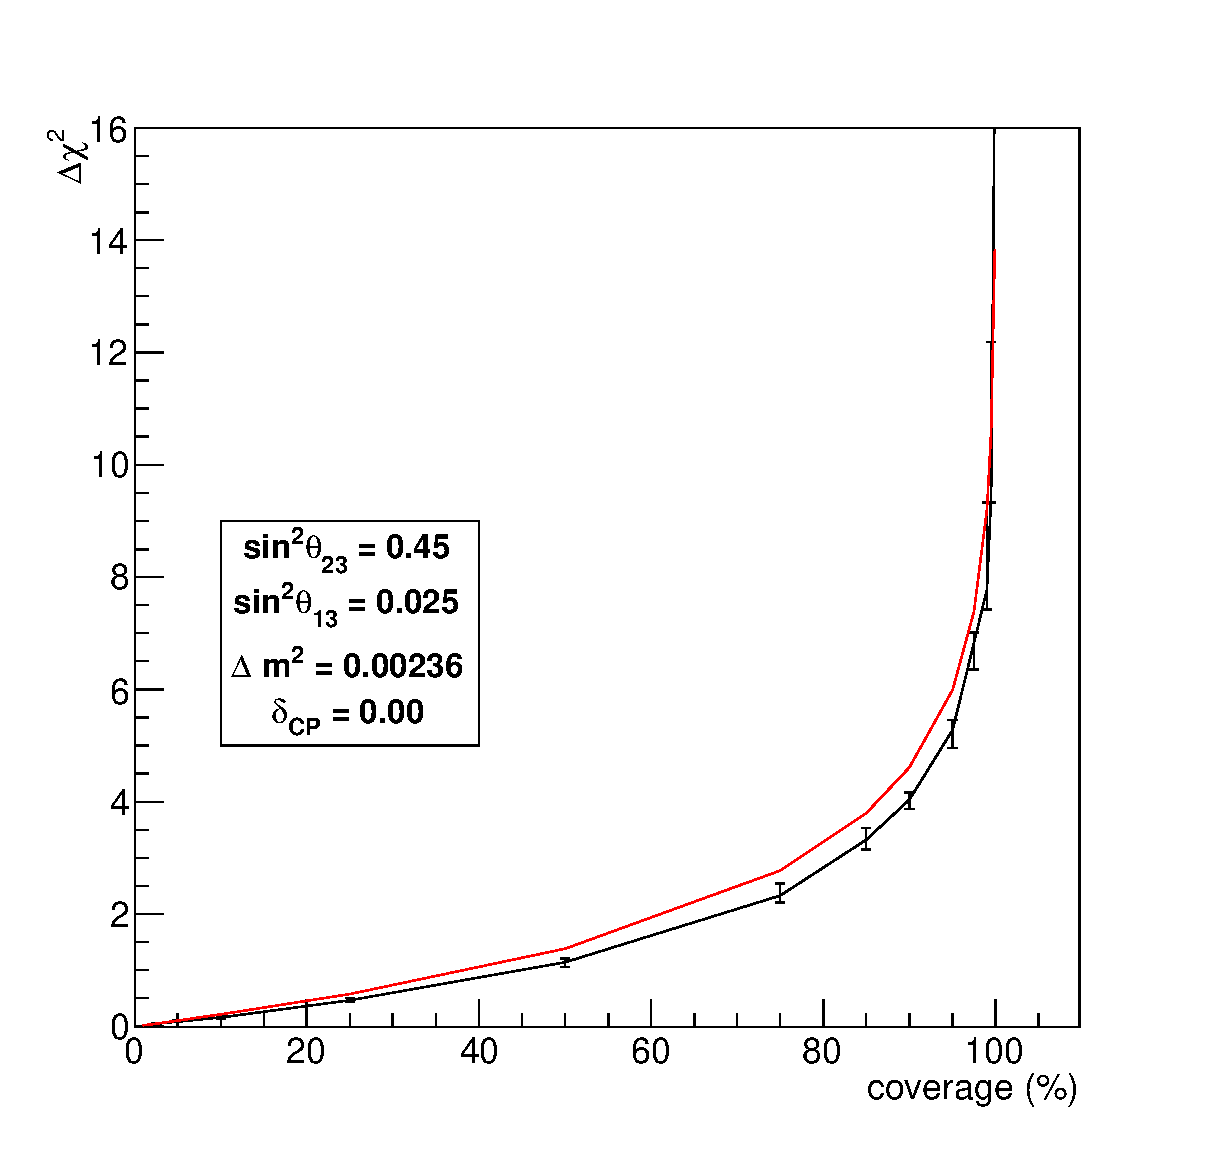
\includegraphics[width=14pc]{./images/appendix/coverage/coverage_study_2D_theta13_theta23_syst_14.eps}
%\center
%\caption {
%    Distribution of $\Delta\chi^{2}$ vs coverage in the ($sin^{2}\theta_{13}$,$sin^{2}\theta_{23}$) parameter space
%  from 1k toy MC experiments generated with the Run 1+2+3 POT
% with statistical fluctuations and systematic variations at the oscillation point indicated in the legend.
%	}
%\label{fig:cov_2D_theta13_theta23_syst_14}
%\end{minipage}
%\hspace{0.03\linewidth}
%\begin{minipage}[t]{0.46\linewidth}
%\center
%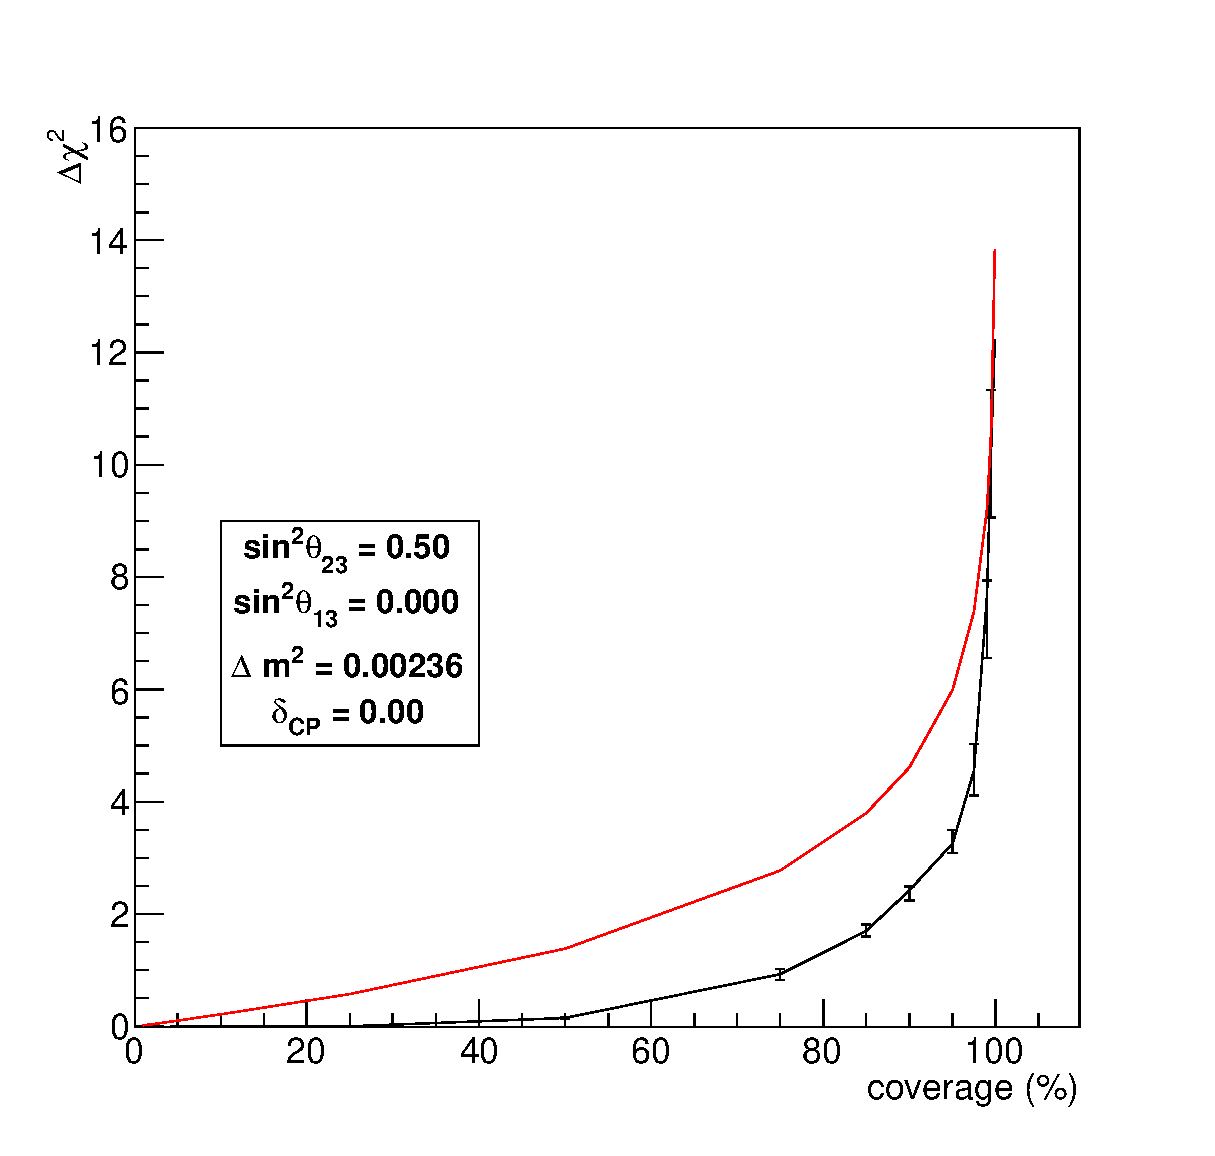
\includegraphics[width=14pc]{./images/appendix/coverage/coverage_study_2D_theta13_theta23_syst_15.eps}
%\center
%\caption {
%  Distribution of $\Delta\chi^{2}$ vs coverage in the ($sin^{2}\theta_{13}$,$sin^{2}\theta_{23}$) parameter space
%  from 1k toy MC experiments generated with the Run 1+2+3 POT
% with statistical fluctuations and systematic variations at the oscillation point indicated in the legend.
%	}
%\label{fig:cov_2D_theta13_theta23_syst_15}
%\end{minipage}
%\vfill
%\vspace*{0.7cm}
%\begin{minipage}[t]{0.46\linewidth}
%\center
%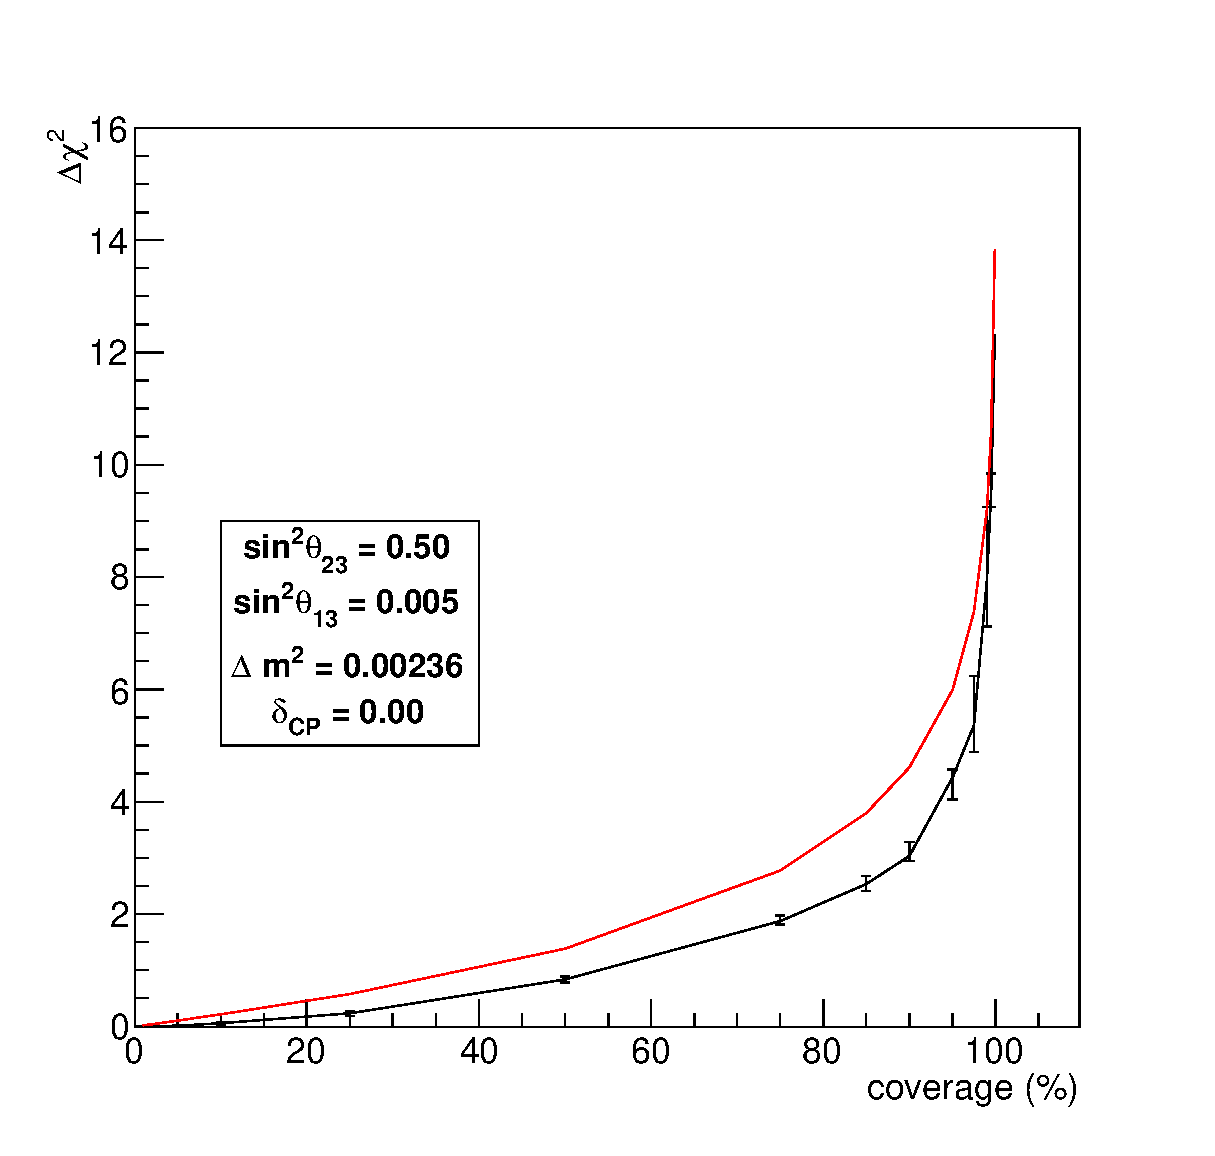
\includegraphics[width=14pc]{./images/appendix/coverage/coverage_study_2D_theta13_theta23_syst_16.eps}
%\center
%\caption {
 %  Distribution of $\Delta\chi^{2}$ vs coverage in the ($sin^{2}\theta_{13}$,$sin^{2}\theta_{23}$) parameter space
 % from 1k toy MC experiments generated with the Run 1+2+3 POT
 %with statistical fluctuations and systematic variations at the oscillation point indicated in the legend.
%	}
%\label{fig:cov_2D_theta13_theta23_syst_16}
%\end{minipage}
%\hspace{0.03\linewidth}
%\begin{minipage}[t]{0.46\linewidth}
%\center
%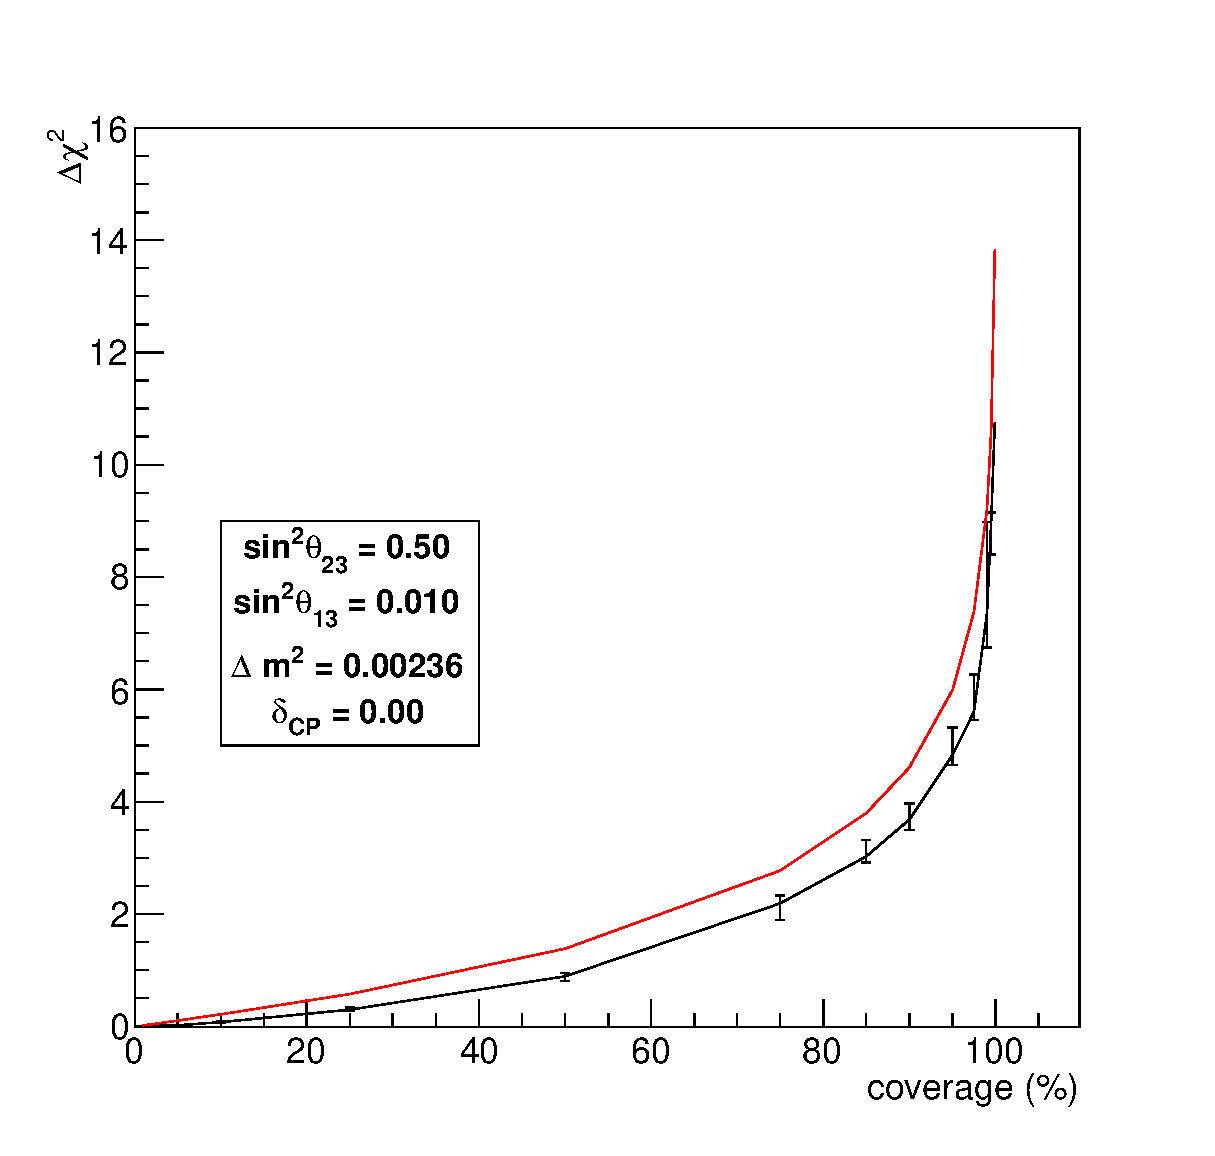
\includegraphics[width=14pc]{./images/appendix/coverage/coverage_study_2D_theta13_theta23_syst_17.eps}
%\center
%\caption {
%    Distribution of $\Delta\chi^{2}$ vs coverage in the ($sin^{2}\theta_{13}$,$sin^{2}\theta_{23}$) parameter space
%  from 1k toy MC experiments generated with the Run 1+2+3 POT
% with statistical fluctuations and systematic variations at the oscillation point indicated in the legend.
%		}
%\label{fig:cov_2D_theta13_theta23_syst_17}
%\end{minipage}
%\end{figure*}
%\end{center}



%\begin{center}
%\begin{figure*}[htb]
%\begin{minipage}[t]{0.46\linewidth}
%\center
%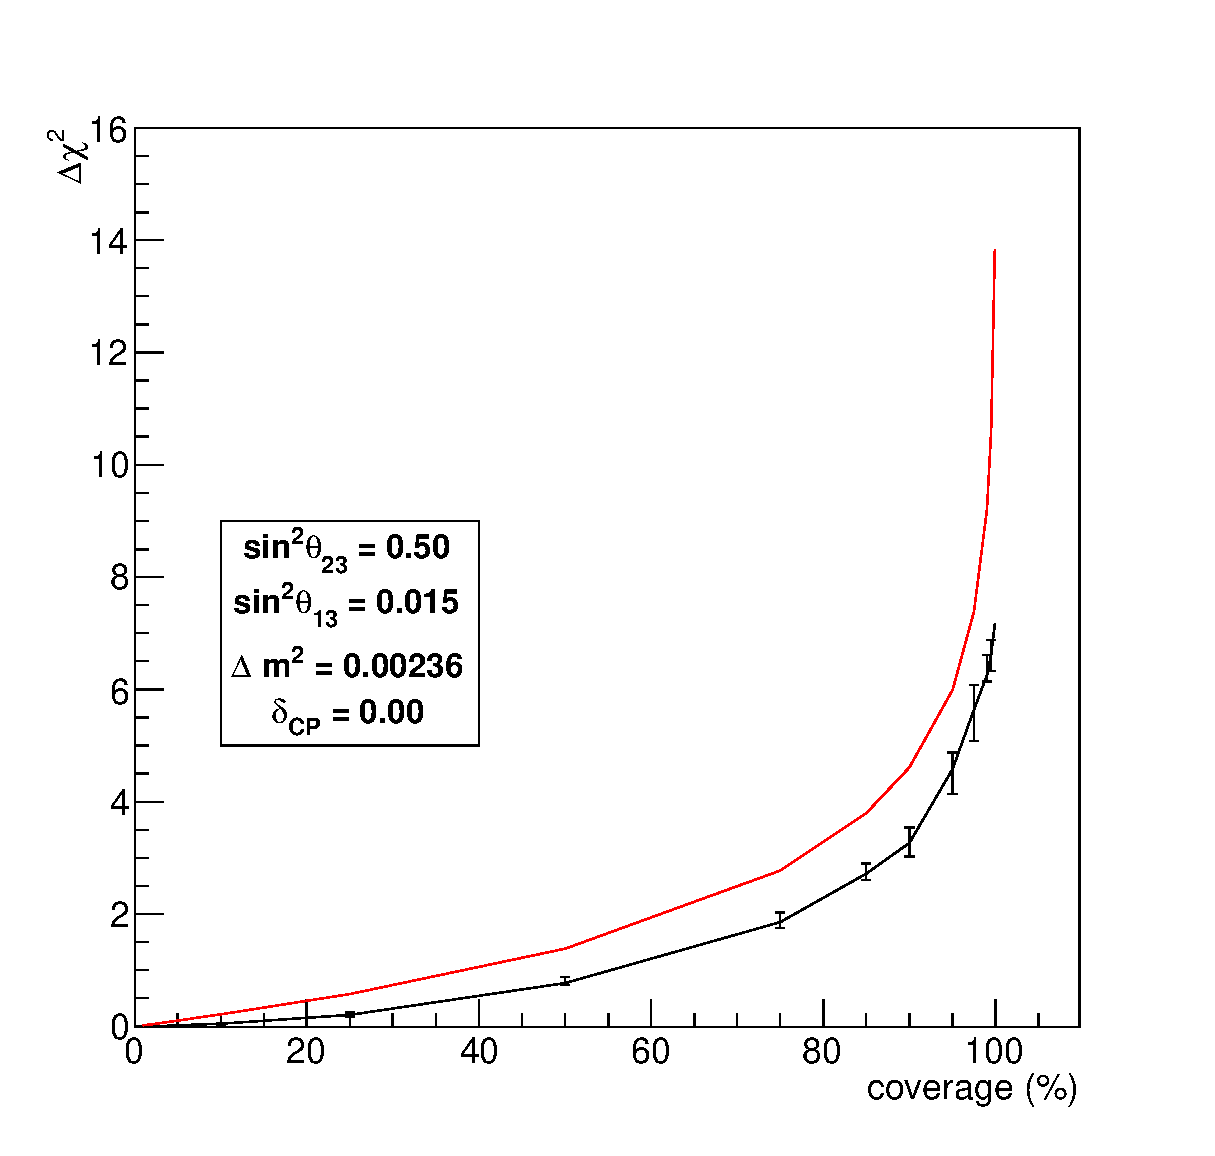
\includegraphics[width=14pc]{./images/appendix/coverage/coverage_study_2D_theta13_theta23_syst_18.eps}
%\center
%\caption {
%    Distribution of $\Delta\chi^{2}$ vs coverage in the ($sin^{2}\theta_{13}$,$sin^{2}\theta_{23}$) parameter space
%  from 1k toy MC experiments generated with the Run 1+2+3 POT
% with statistical fluctuations and systematic variations at the oscillation point indicated in the legend.
%  }
%\label{fig:cov_2D_theta13_theta23_syst_18}
%\end{minipage}
%\hspace{0.03\linewidth}
%\begin{minipage}[t]{0.46\linewidth}
%\center
%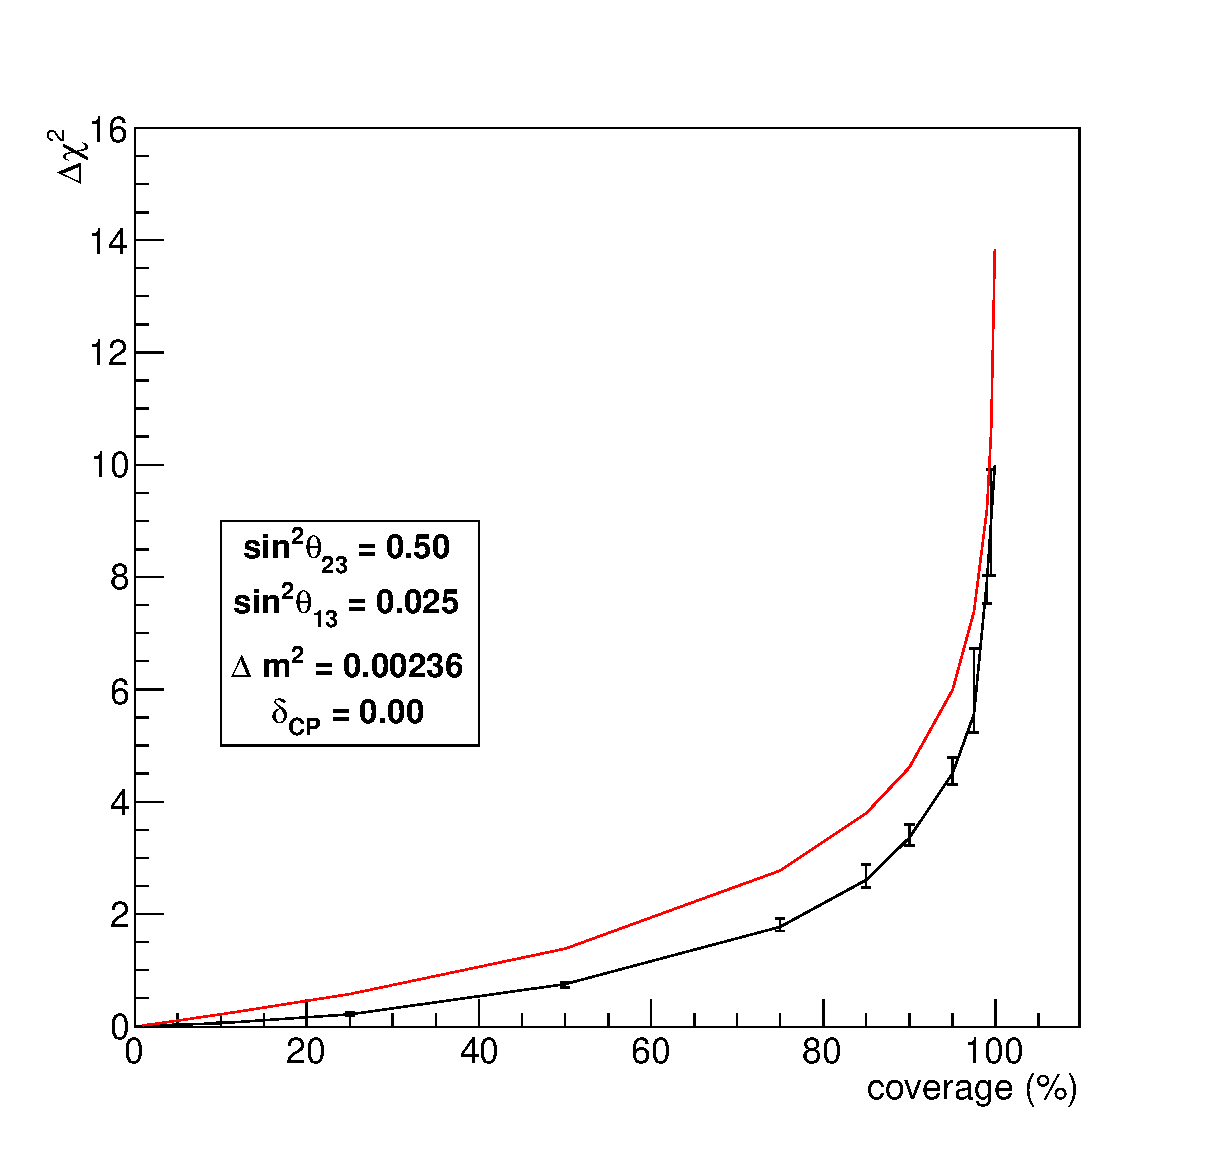
\includegraphics[width=14pc]{./images/appendix/coverage/coverage_study_2D_theta13_theta23_syst_19.eps}
%\center
%\caption {
%   Distribution of $\Delta\chi^{2}$ vs coverage in the ($sin^{2}\theta_{13}$,$sin^{2}\theta_{23}$) parameter space
%  from 1k toy MC experiments generated with the Run 1+2+3 POT
% with statistical fluctuations and systematic variations at the oscillation point indicated in the legend.
%  	}
%\label{fig:cov_2D_theta13_theta23_syst_19}
%\end{minipage}
%\vfill
%\vspace*{0.7cm}

\begin{center}
\begin{figure*}[htb]
\begin{minipage}[t]{0.46\linewidth}
\center
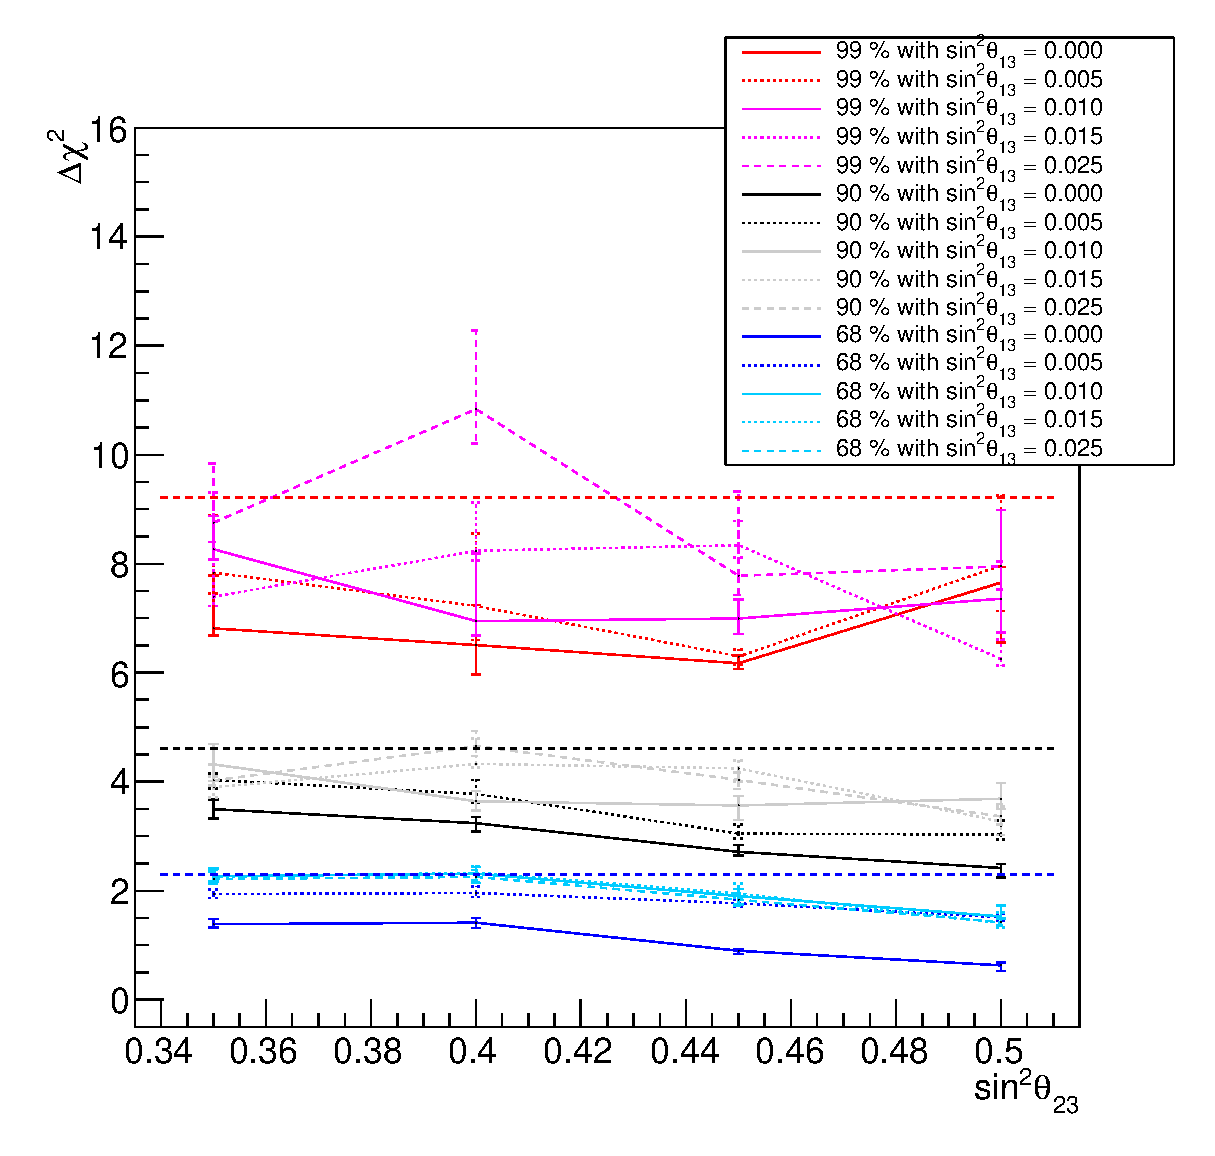
\includegraphics[width=14pc]{./images/appendix/coverage/coverage_study_2D_theta13_theta23_syst_all_1.eps}
\center
\caption {
    Summary of values of $\Delta\chi^{2}$ at 99\%, 90\% and 68\% confidence intervals in the 2D parameter space ($sin^{2}\theta_{13}$,$sin^{2}\theta_{23}$) vs the value of $sin^{2}\theta_{23}$.
True input values for the other oscillation parameters:
$|\Delta m^{2}| = 2.36 \times 10^{-3}$ and
        $\delta_{CP}$   = 0.
	}
\label{fig:cov_2D_theta13_theta23_syst_all_1}
\end{minipage}
\hspace{0.03\linewidth}
\begin{minipage}[t]{0.46\linewidth}
\center
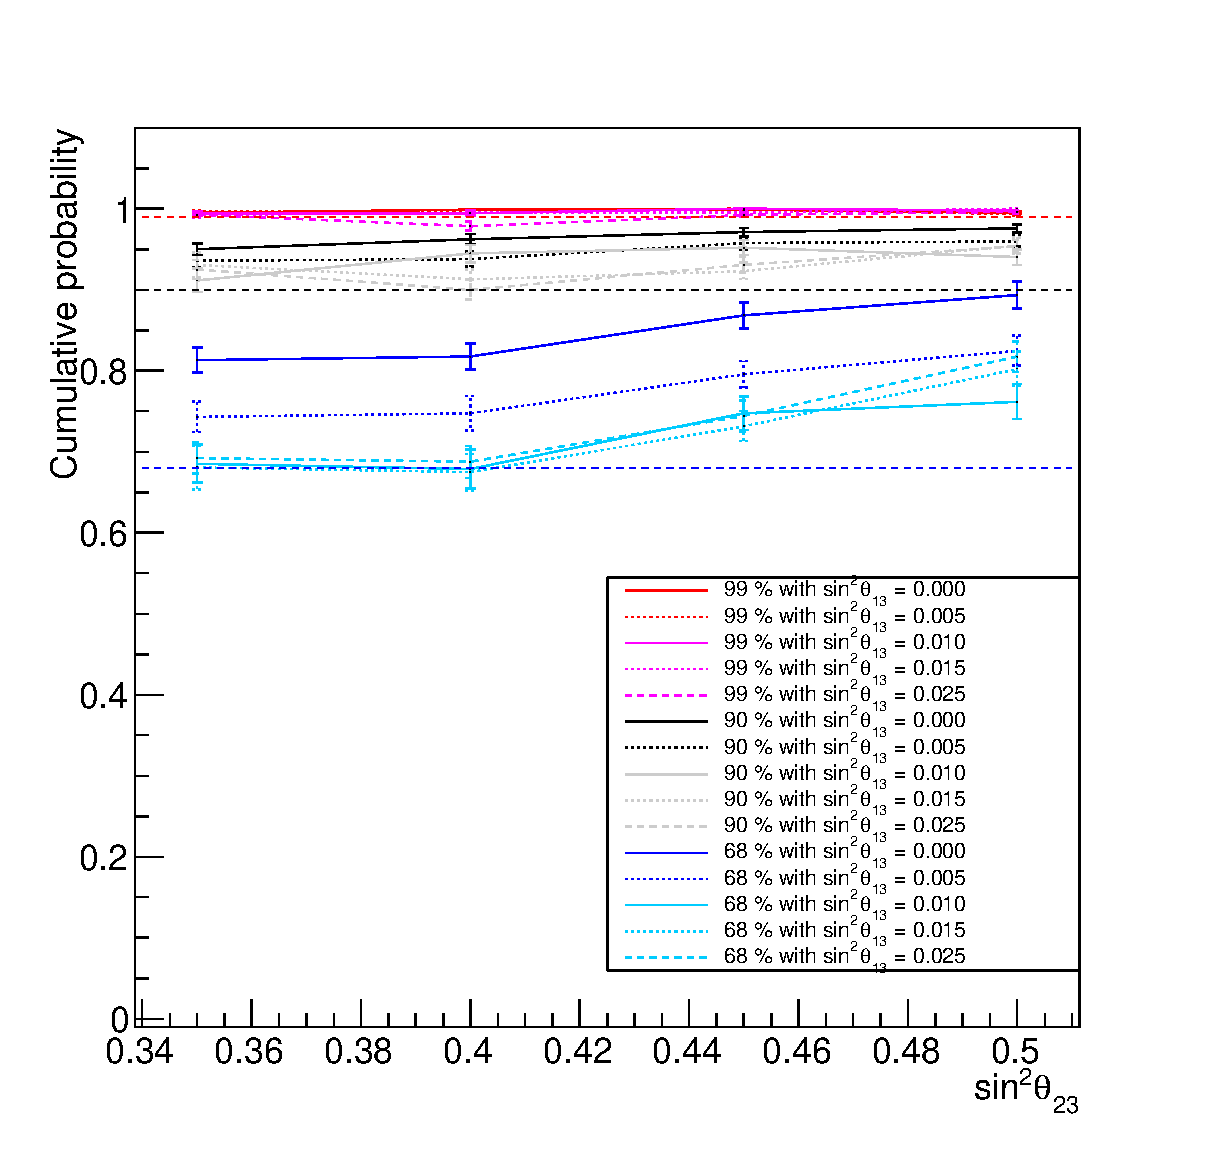
\includegraphics[width=14pc]{./images/appendix/coverage/coverage_study_2D_theta13_theta23_syst_new_all_2.eps}
\center
\caption {
    Summary of values of cumulative probability  for $\Delta\chi^{2}=9.21$ (canonical value for 99\%), $\Delta\chi^{2}=4.61$ (canonical value for 90\%) and $\Delta\chi^{2}=2.30$ (canonical value for 68\%) in the 2D parameter space ($sin^{2}\theta_{13}$,$sin^{2}\theta_{23}$) vs the value of $sin^{2}\theta_{23}$.
True input values for the other oscillation parameters:
$|\Delta m^{2}| = 2.36 \times 10^{-3}$ and
        $\delta_{CP}$   = 0.
	}
\label{fig:prob_2D_theta13_theta23_syst_all_1}
\end{minipage}
\vfill
\vspace*{0.7cm}
\begin{minipage}[t]{0.46\linewidth}
\center
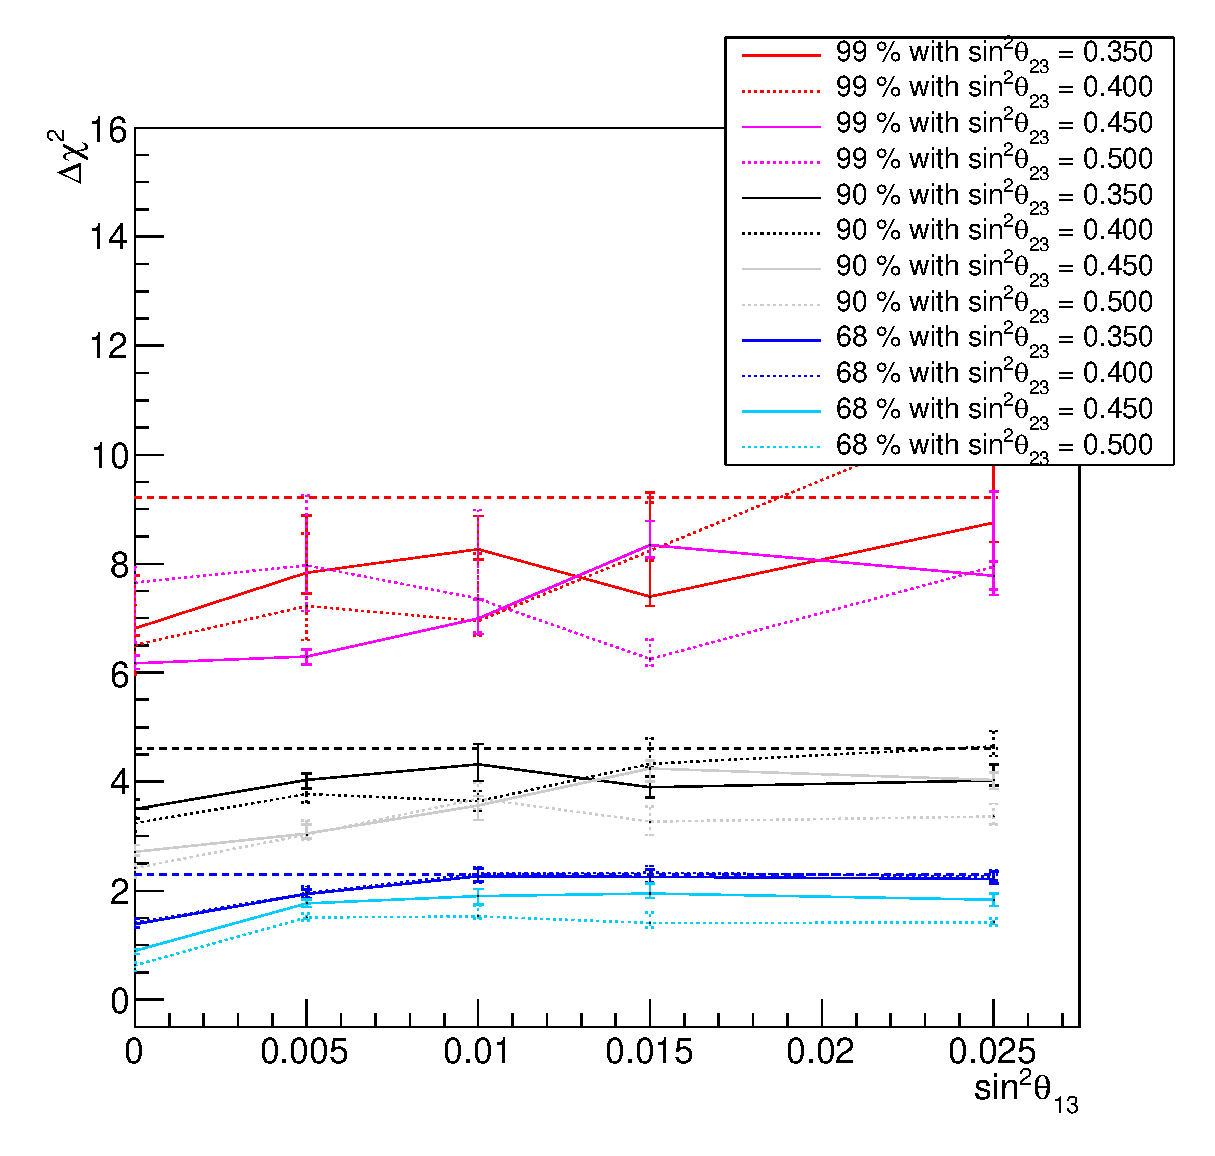
\includegraphics[width=14pc]{./images/appendix/coverage/coverage_study_2D_theta13_theta23_syst_all_2.eps}
\center
\caption {
    Summary of values of $\Delta\chi^{2}$ at 99\%, 90\% and 68\% confidence intervals in the 2D parameter space ($sin^{2}\theta_{13}$,$sin^{2}\theta_{23}$) vs the value of $sin^{2}\theta_{13}$.
True input values for the other oscillation parameters:
$|\Delta m^{2}| = 2.36 \times 10^{-3}$ and
        $\delta_{CP}$   = 0.
		}
\label{fig:cov_2D_theta13_theta23_syst_all_2}
\end{minipage}
\hspace{0.03\linewidth}
\begin{minipage}[t]{0.46\linewidth}
\center
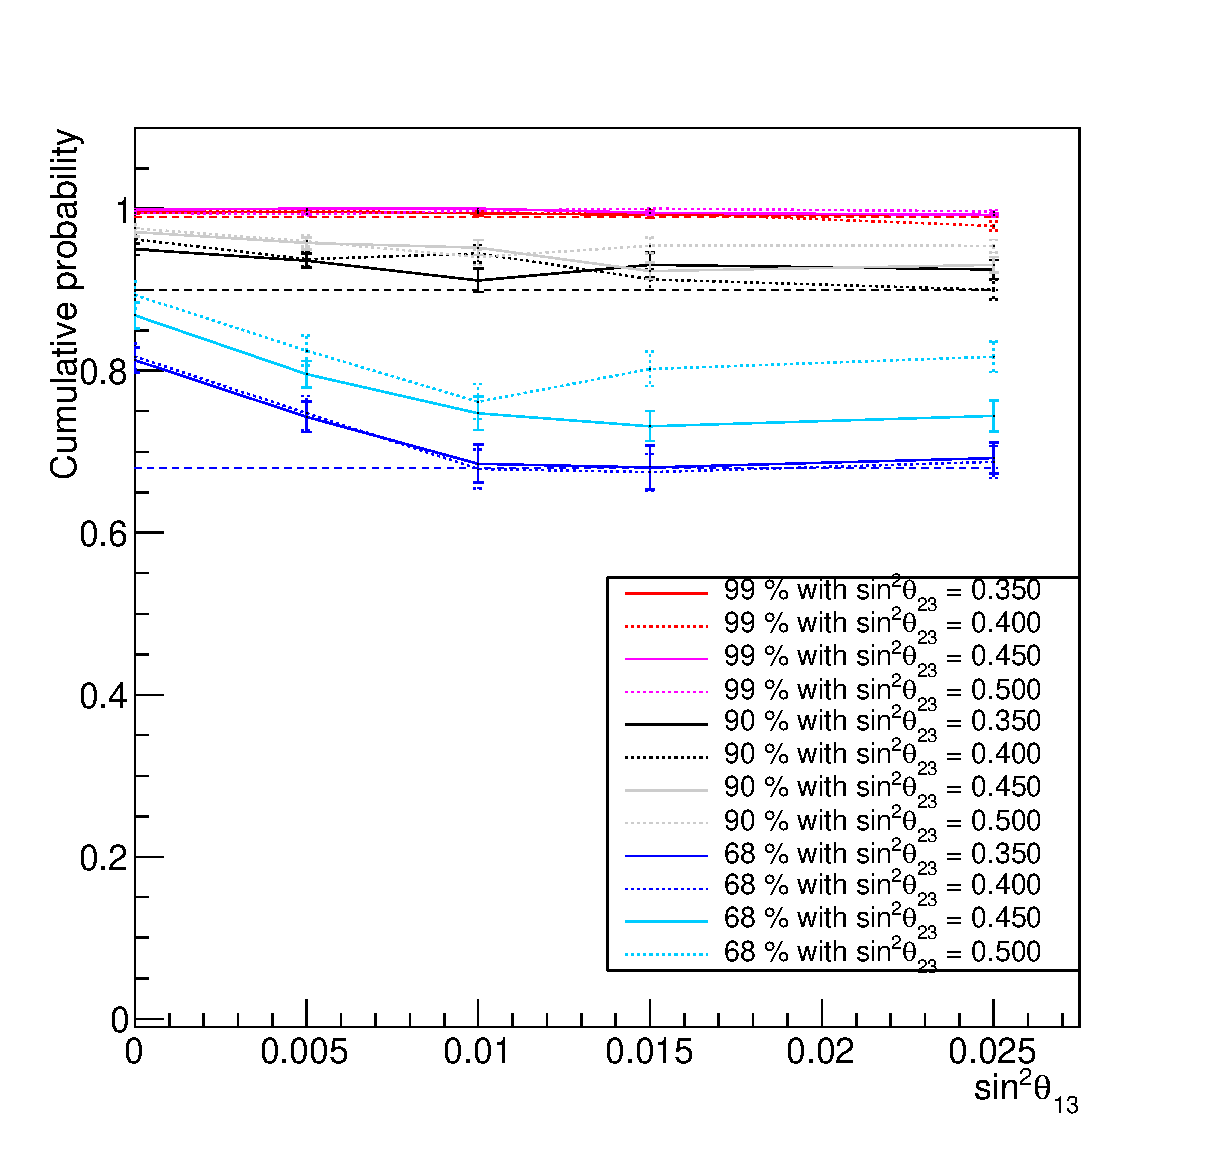
\includegraphics[width=14pc]{./images/appendix/coverage/coverage_study_2D_theta13_theta23_syst_new_all_1.eps}
\center
\caption {
    Summary of values of cumulative probability  for $\Delta\chi^{2}=9.21$ (canonical value for 99\%), $\Delta\chi^{2}=4.61$ (canonical value for 90\%) and $\Delta\chi^{2}=2.30$ (canonical value for 68\%) in the 2D parameter space ($sin^{2}\theta_{13}$,$sin^{2}\theta_{23}$) vs the value of $sin^{2}\theta_{13}$.
True input values for the other oscillation parameters:
$|\Delta m^{2}| = 2.36 \times 10^{-3}$ and
        $\delta_{CP}$   = 0.
	}
\label{fig:prob_2D_theta13_theta23_syst_all_2}
\end{minipage}
\end{figure*}
\end{center}

\begin{center}
\begin{figure*}[htb]
\begin{minipage}[t]{0.46\linewidth}
\center
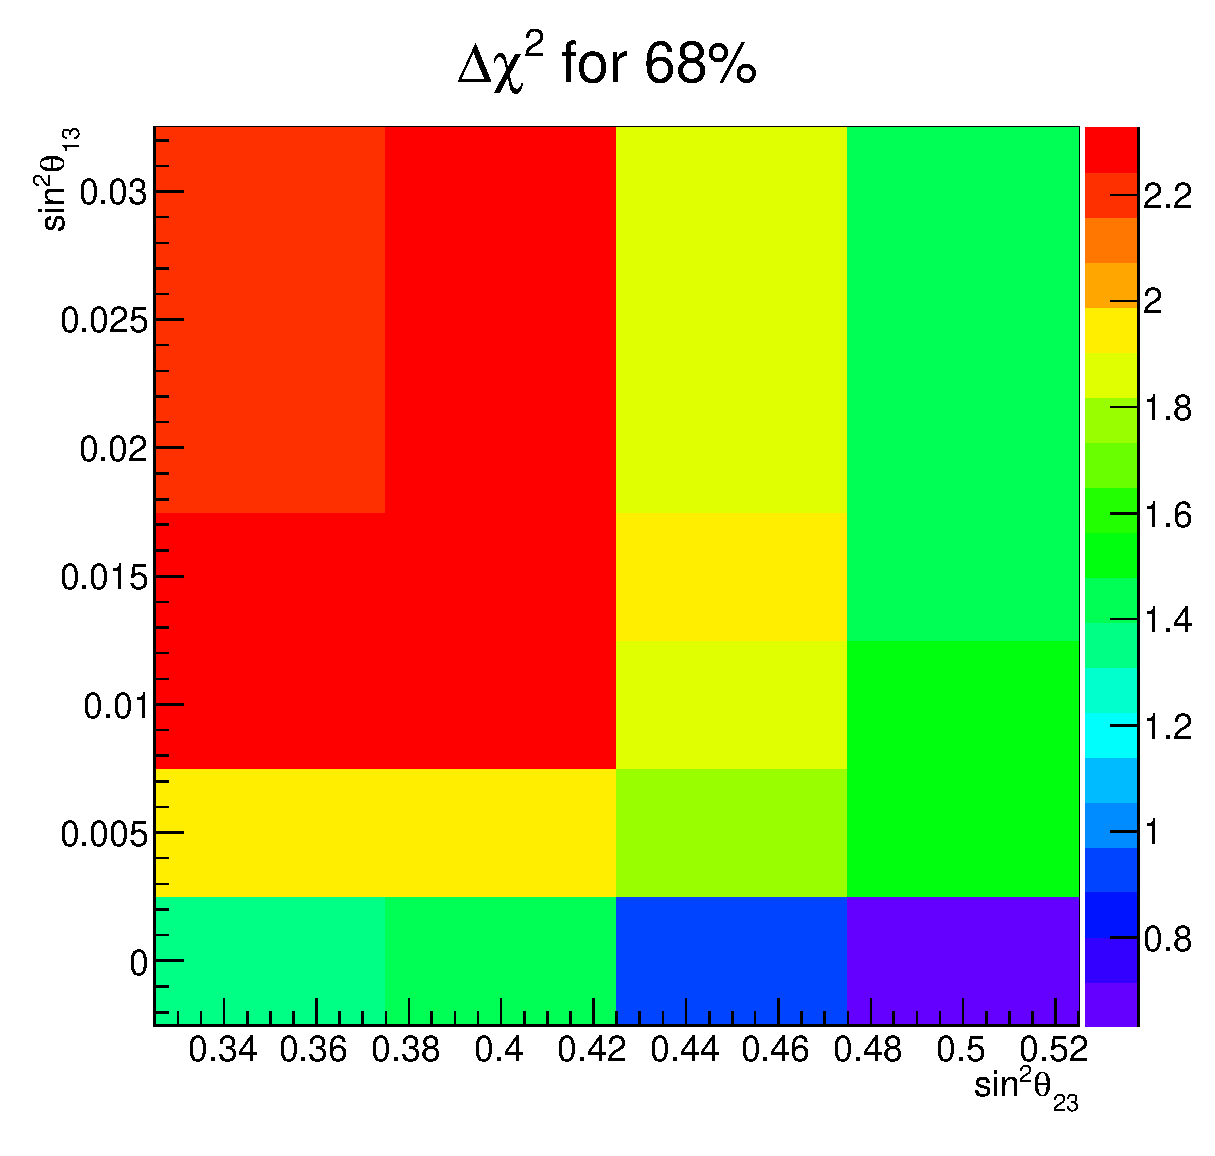
\includegraphics[width=14pc]{./images/appendix/coverage/coverage_study_2D_theta13_theta23_syst_68.eps}
\caption {
    Summary of values of $\Delta\chi^{2}$ at 68\% confidence intervals in Z axis (color) in the 2D parameter space ($sin^{2}\theta_{13}$,$sin^{2}\theta_{23}$) vs the value of $sin^{2}\theta_{23}$ in X axis and $sin^{2}\theta_{13}$ in Y axis. 
True input values for the other oscillation parameters:
$|\Delta m^{2}| = 2.36 \times 10^{-3}$ and
        $\delta_{CP}$   = 0.
	}
\label{fig:cov_2D_theta13_theta23_syst_68}
\end{minipage}
\hspace{0.03\linewidth}
\begin{minipage}[t]{0.46\linewidth}
\center
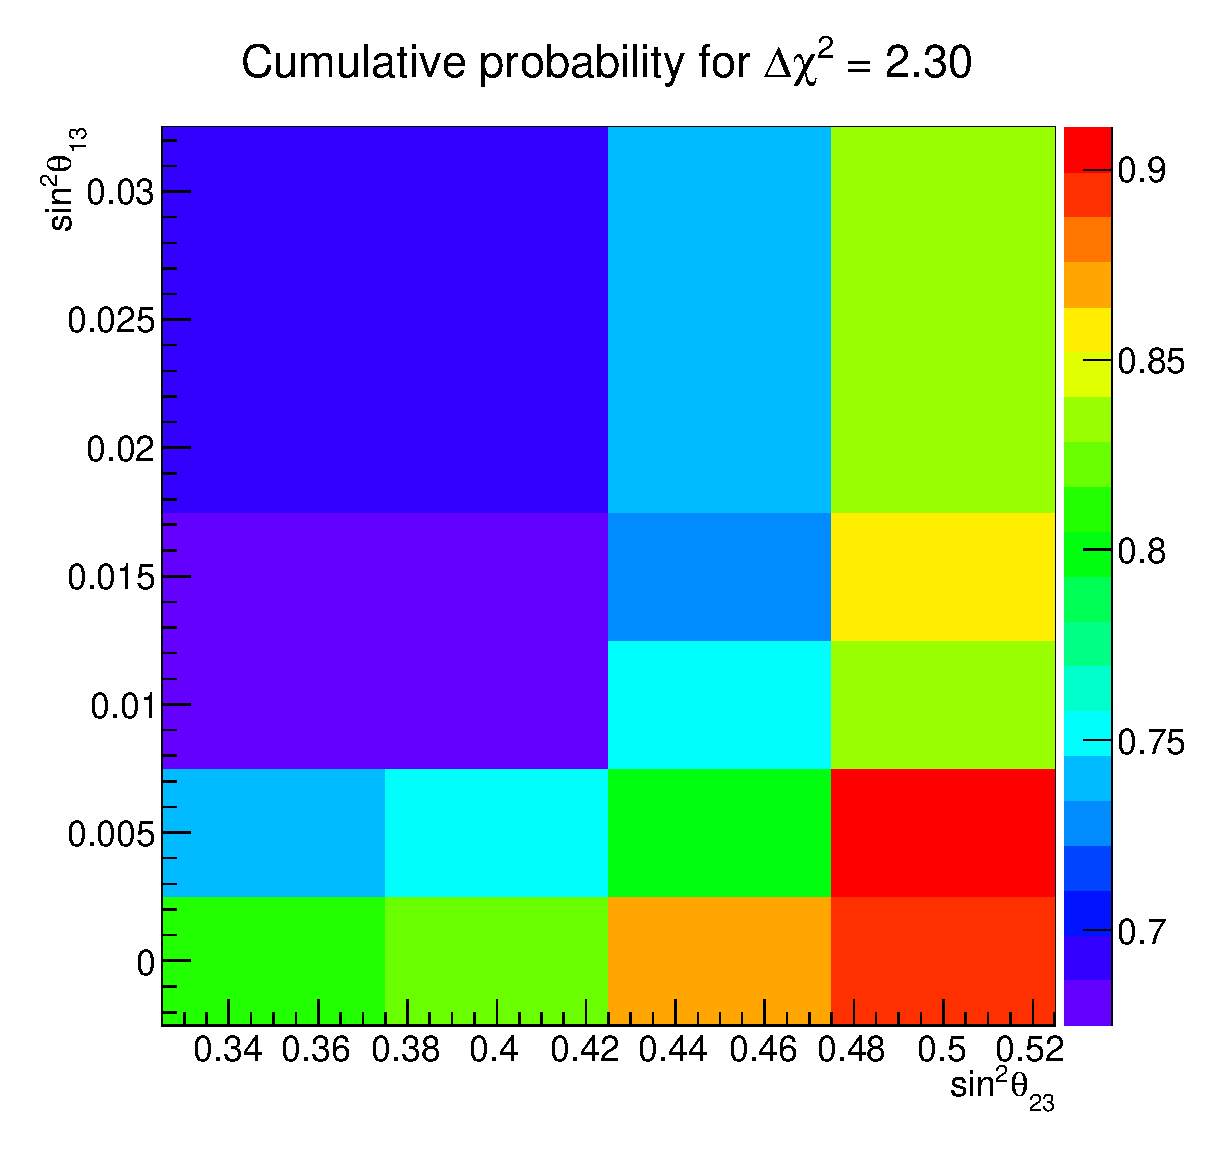
\includegraphics[width=14pc]{./images/appendix/coverage/coverage_study_2D_theta13_theta23_syst_new_68.eps}
\caption {
    Summary of values of cumulative probability at $\Delta\chi^{2} = 2.30$ in Z axis (color) in the 2D parameter space ($sin^{2}\theta_{13}$,$sin^{2}\theta_{23}$) vs the value of $sin^{2}\theta_{23}$ in X axis and $sin^{2}\theta_{13}$ in Y axis. 
True input values for the other oscillation parameters:
$|\Delta m^{2}| = 2.36 \times 10^{-3}$ and
        $\delta_{CP}$   = 0.
	}
\label{fig:prob_2D_theta13_theta23_syst_68}
\end{minipage}
\vfill
\vspace*{0.7cm}
\begin{minipage}[t]{0.46\linewidth}
\center
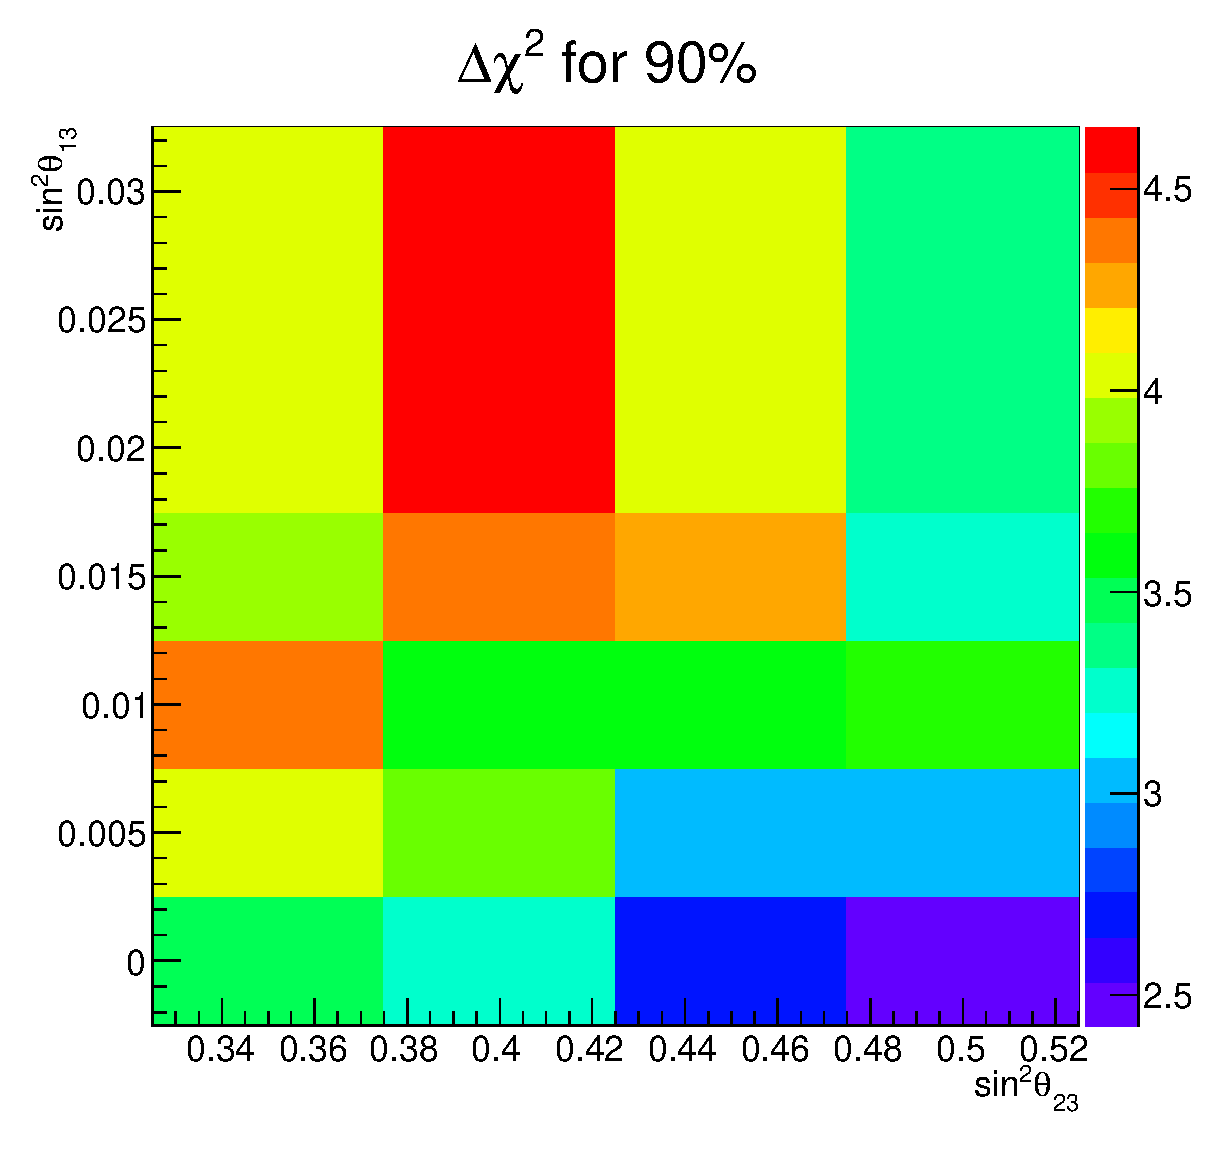
\includegraphics[width=14pc]{./images/appendix/coverage/coverage_study_2D_theta13_theta23_syst_90.eps}
\caption {
   Summary of values of $\Delta\chi^{2}$ at 90\% confidence intervals in Z axis (color) in the 2D parameter space ($sin^{2}\theta_{13}$,$sin^{2}\theta_{23}$) vs the value of $sin^{2}\theta_{23}$ in X axis and $sin^{2}\theta_{13}$ in Y axis. 
True input values for the other oscillation parameters:
$|\Delta m^{2}| = 2.36 \times 10^{-3}$ and
        $\delta_{CP}$   = 0.
		}
\label{fig:cov_2D_theta13_theta23_syst_90}
\end{minipage}
\hspace{0.03\linewidth}
\begin{minipage}[t]{0.46\linewidth}
\center
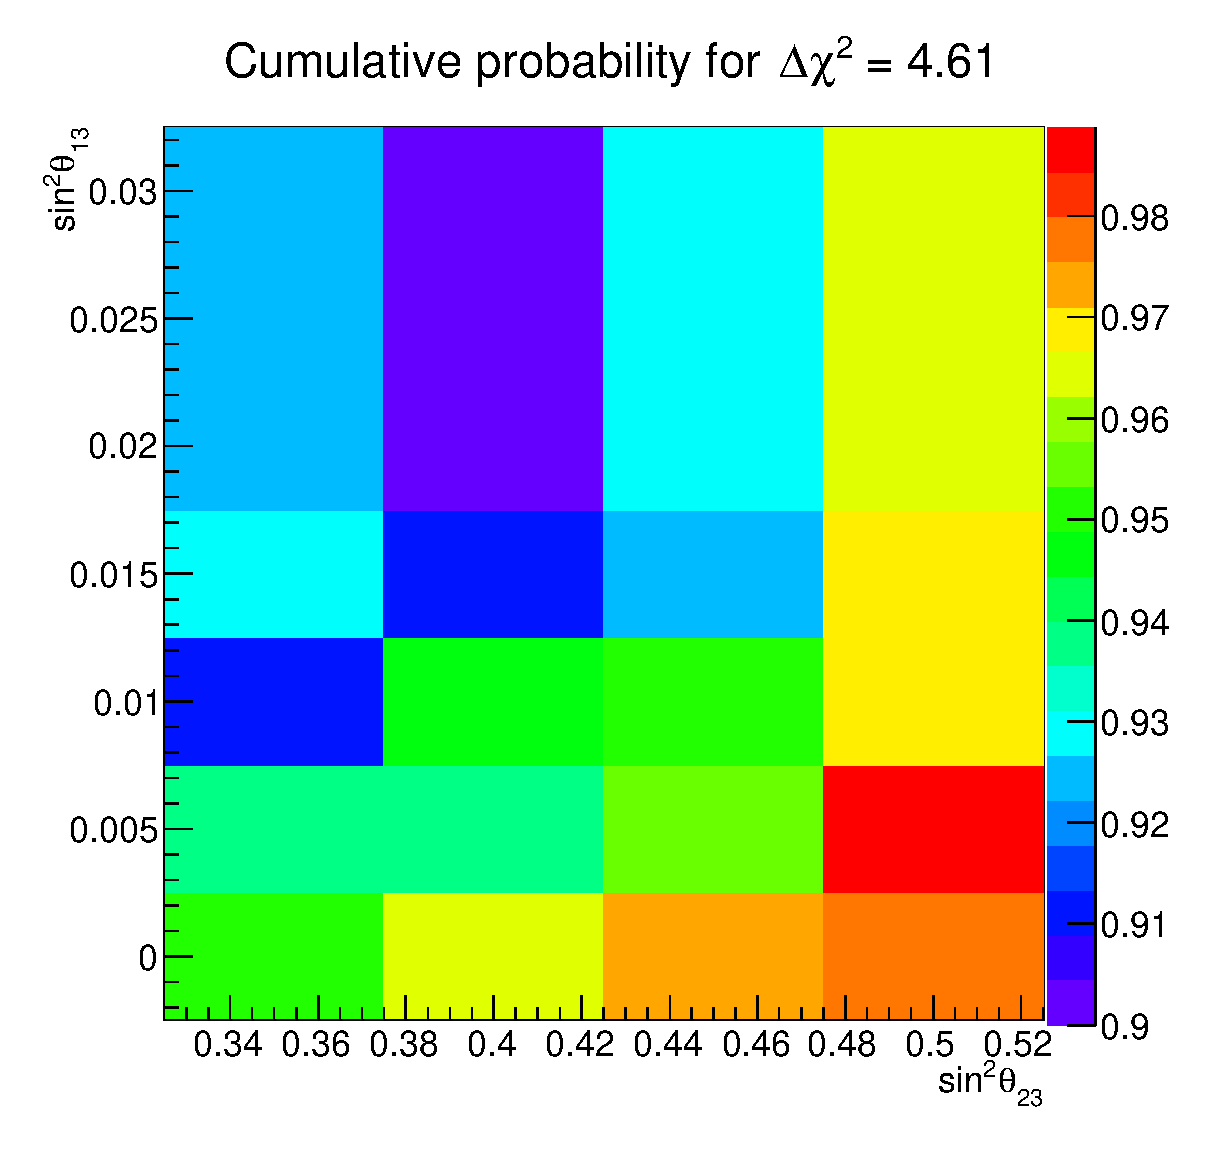
\includegraphics[width=14pc]{./images/appendix/coverage/coverage_study_2D_theta13_theta23_syst_new_90.eps}
\caption {
    Summary of values of cumulative probability at $\Delta\chi^{2} = 4.61$ in Z axis (color) in the 2D parameter space ($sin^{2}\theta_{13}$,$sin^{2}\theta_{23}$) vs the value of $sin^{2}\theta_{23}$ in X axis and $sin^{2}\theta_{13}$ in Y axis. 
True input values for the other oscillation parameters:
$|\Delta m^{2}| = 2.36 \times 10^{-3}$ and
        $\delta_{CP}$   = 0.
	}
\label{fig:prob_2D_theta13_theta23_syst_90}
\end{minipage}
\vfill
\vspace*{0.7cm}
\center
\begin{minipage}[t]{0.46\linewidth}
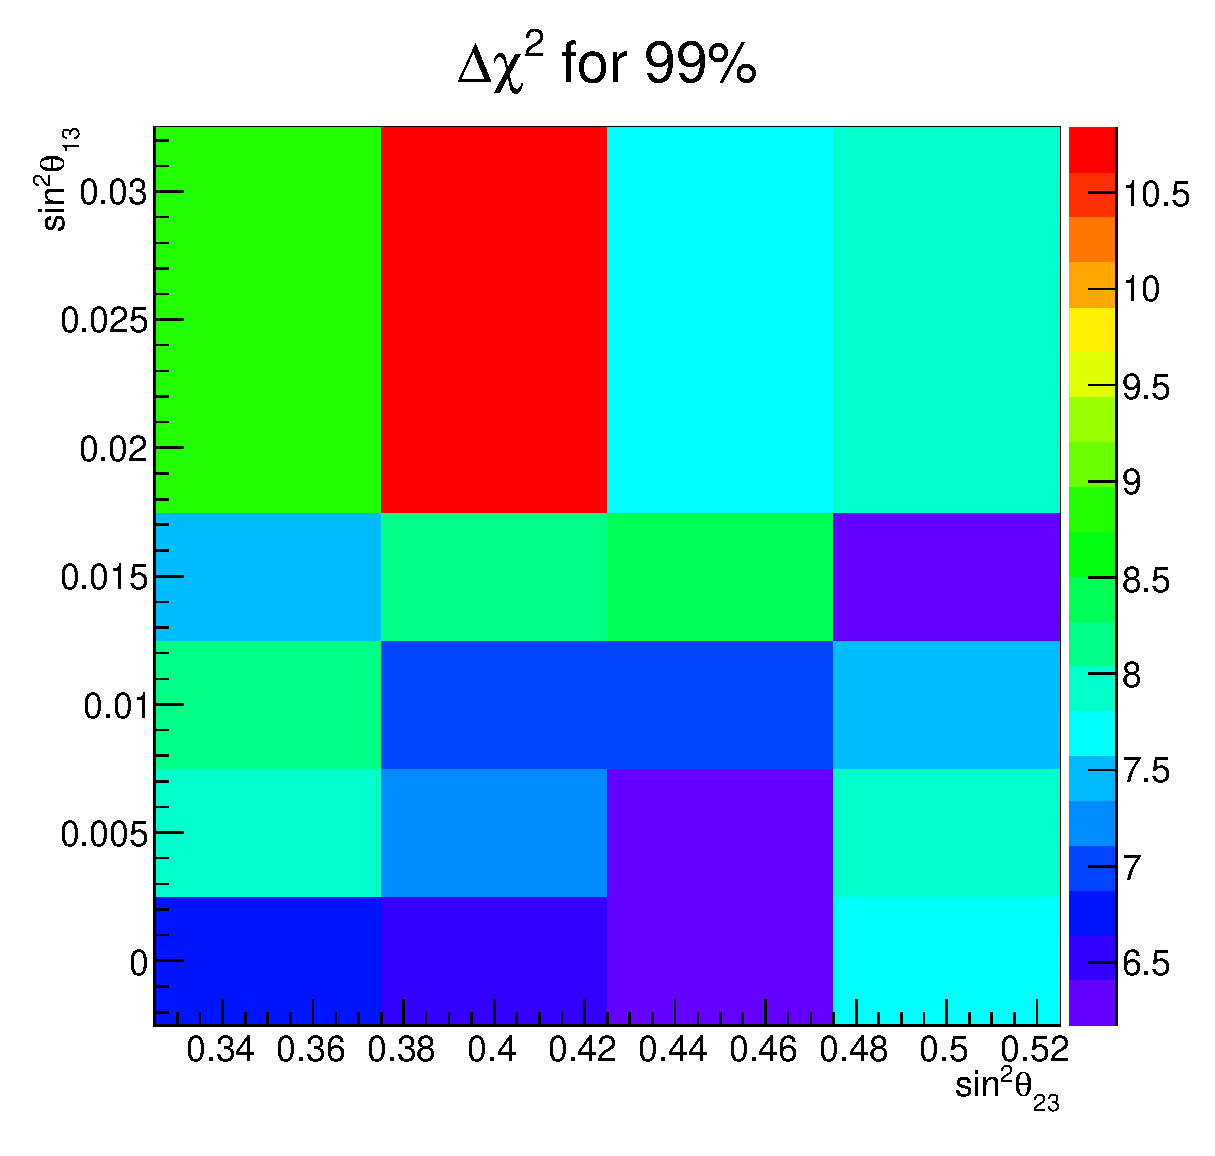
\includegraphics[width=14pc]{./images/appendix/coverage/coverage_study_2D_theta13_theta23_syst_99.eps}
\caption {
    Summary of values of $\Delta\chi^{2}$ at 99\% confidence intervals in Z axis (color) in the 2D parameter space ($sin^{2}\theta_{13}$,$sin^{2}\theta_{23}$) vs the value of $sin^{2}\theta_{23}$ in X axis and $sin^{2}\theta_{13}$ in Y axis. 
True input values for the other oscillation parameters:
$|\Delta m^{2}| = 2.36 \times 10^{-3}$ and
        $\delta_{CP}$   = 0.
	}
\label{fig:cov_2D_theta13_theta23_syst_99}
\end{minipage}
\hspace{0.03\linewidth}
\begin{minipage}[t]{0.46\linewidth}
\center
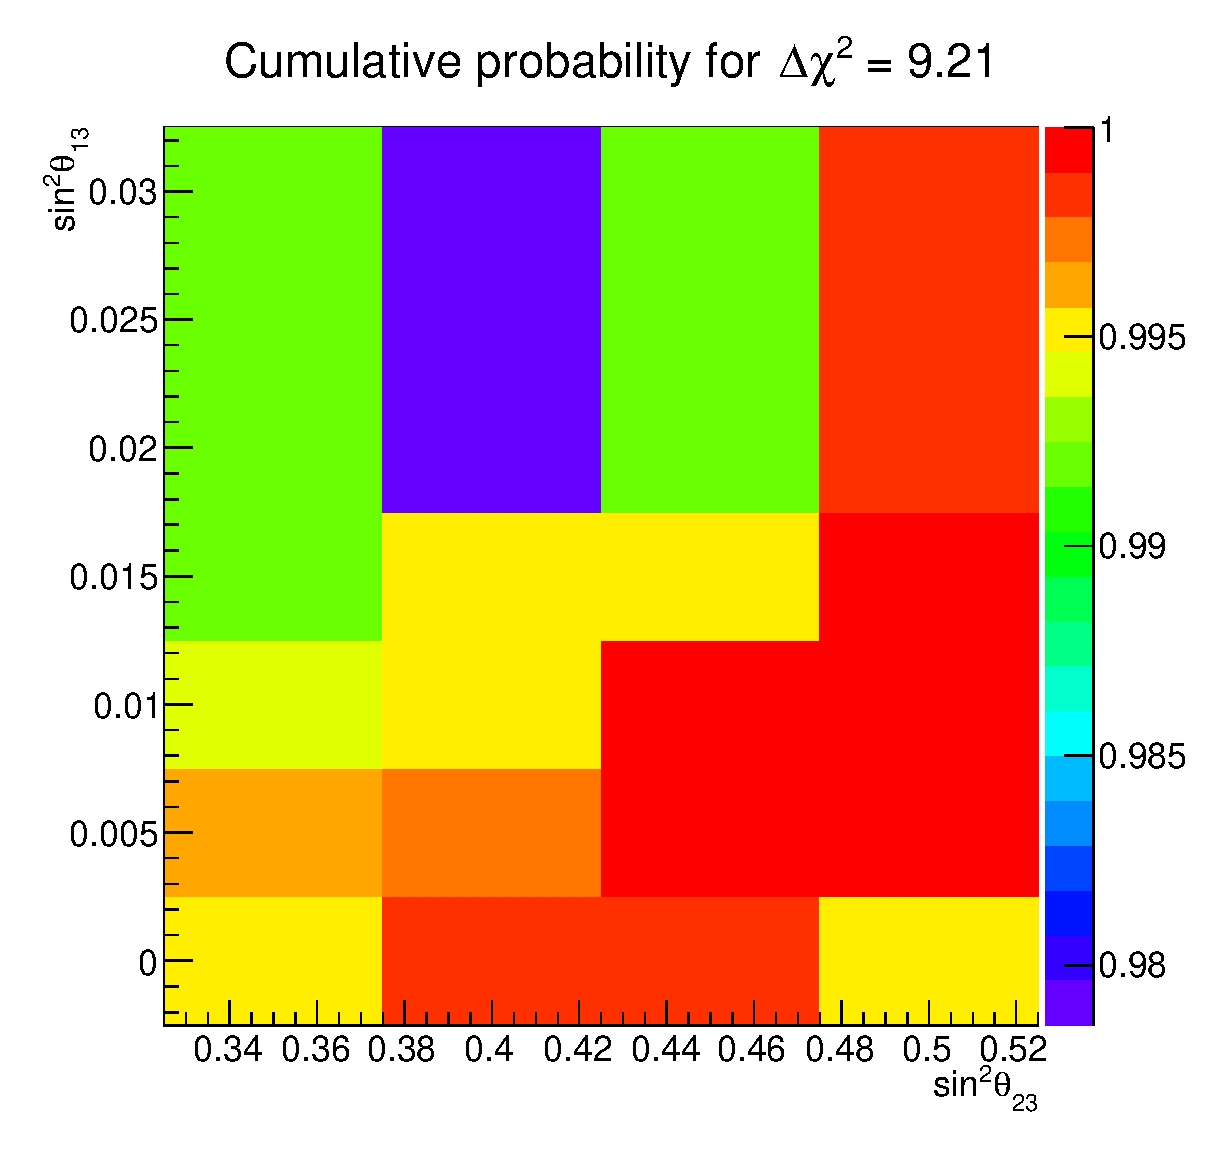
\includegraphics[width=14pc]{./images/appendix/coverage/coverage_study_2D_theta13_theta23_syst_new_99.eps}
\caption {
    Summary of values of cumulative probability at $\Delta\chi^{2} = 9.21$ in Z axis (color) in the 2D parameter space ($sin^{2}\theta_{13}$,$sin^{2}\theta_{23}$) vs the value of $sin^{2}\theta_{23}$ in X axis and $sin^{2}\theta_{13}$ in Y axis. 
True input values for the other oscillation parameters:
$|\Delta m^{2}| = 2.36 \times 10^{-3}$ and
        $\delta_{CP}$   = 0.
	}
\label{fig:prob_2D_theta13_theta23_syst_99}
\end{minipage}
\end{figure*}
\end{center}




\clearpage
\subsection{Coverage studies in 2D including the other oscillation parameters in the fit}
\label{app:cov:systosc}

In this subsection the studies are done for the same oscillation points in the 2D parameter spaces seen previously,
but including the other two oscillation parameters in the fit in order to reproduce the same scenario as the fits done for the results in this analysis. The studies will be presented with statistical fluctuations only and with systematic variations added. 
In both cases none of the oscillation parameters remains fixed to its true value now: those that are not under study are now 
fitted in both fits as explained at the beginning of the section. So the procedure is as follows (similarly for statistical fluctuations only, removing systematics from both fits):

\begin{itemize}
\item{At a certain oscillation point, 1k toy experiments were created with statistical fluctuations and random systematic variations.}
\item{A first value of $\chi^{2}$ ($\chi^{2} _{init}$) was obtained for each toy experiment fixing the oscillation parameters under study to the true input values and fitting the systematic parameters and the other two oscillation parameters.}
\item{A second fit was performed for each toy experiment fitting the four oscillation parameters and systematic errors, obtaining $\chi^{2} _{bf}$.}
\item{The value of $\Delta\chi^{2}$ was calculated for each toy experiment as the difference $\Delta\chi^{2} = \chi^{2}_{init} - \chi^{2}_{bf}$, and the plots explained for the tests with statistical fluctuations only were made.}
\end{itemize}

In this subsection only summary plots are presented. For the 2D parameter space ($sin^{2}\theta_{23}$,$|\Delta m^{2}|$),
Figures \ref{fig:cov_2D_theta23_dmsq_stats_osc_all}-\ref{fig:prob_2D_theta23_dmsq_stats_osc_all} and \ref{fig:cov_2D_theta23_dmsq_syst_osc_all}-\ref{fig:prob_2D_theta23_dmsq_syst_osc_all} are the summary plots with statistical fluctuations only and including systematic variations respectively. 
The same for the 2D parameter space ($sin^{2}\theta_{13}$,$|\Delta m^{2}|$) in Figs. \ref{fig:cov_2D_theta13_dmsq_stats_osc_all}-\ref{fig:prob_2D_theta13_dmsq_stats_osc_all} and \ref{fig:cov_2D_theta13_dmsq_syst_osc_all}-\ref{fig:prob_2D_theta13_dmsq_syst_osc_all} and Figs. \ref{fig:cov_2D_theta13_deltacp_stats_osc_all}-\ref{fig:prob_2D_theta13_deltacp_stats_osc_all} and\ref{fig:cov_2D_theta13_deltacp_syst_osc_all}-\ref{fig:prob_2D_theta13_deltacp_syst_osc_all} for the 2D parameter space ($sin^{2}\theta_{13}$,$\delta_{CP}$).

For the 2D parameter space ($sin^{2}\theta_{13}$,$sin^{2}\theta_{23}$) summaries are presented in Figs. 
\ref{fig:cov_2D_theta13_theta23_stats_osc_all_1}-\ref{fig:prob_2D_theta13_theta23_stats_osc_all_1} and \ref{fig:cov_2D_theta13_theta23_stats_osc_all_2}-\ref{fig:prob_2D_theta13_theta23_stats_osc_all_2} with statistical fluctuations only and in Figs. \ref{fig:cov_2D_theta13_theta23_syst_osc_all_1}-\ref{fig:prob_2D_theta13_theta23_syst_osc_all_1} and \ref{fig:cov_2D_theta13_theta23_syst_osc_all_2}-\ref{fig:prob_2D_theta13_theta23_syst_osc_all_2} with systematic variations, showing the values of $\Delta\chi^{2}$ or the cumulative probability vs $sin^{2}\theta_{23}$ and $sin^{2}\theta_{13}$. 
Then a summary is presented with the value of $\Delta\chi^{2}$ in Z axis (color) vs $sin^{2}\theta_{23}$ in X axis and $sin^{2}\theta_{13}$ in Y axis at 68\% confidence interval in Figs.\ref{fig:cov_2D_theta13_theta23_stats_osc_68} and \ref{fig:cov_2D_theta13_theta23_syst_osc_68}, at 90\% confidence interval in Figs. \ref{fig:cov_2D_theta13_theta23_stats_osc_90} and \ref{fig:cov_2D_theta13_theta23_syst_osc_90} and at 99\%  confidence interval in Figs. \ref{fig:cov_2D_theta13_theta23_stats_osc_99} and \ref{fig:cov_2D_theta13_theta23_syst_osc_99},
and summary plots with the value of the cumulative probability in Z axis (color) vs $sin^{2}\theta_{23}$ in X axis and $sin^{2}\theta_{13}$ in Y axis are presented in \ref{fig:prob_2D_theta13_theta23_stats_osc_68}, etc. 

Results obtained in this section present a general overcoverage. 
This behaviour seems to be independent of the addition of systematic fluctuations, appearing the same overcoverage with statistical fluctuations only, as can be clearly observed when comparing both kind of plots (for instance \ref{fig:cov_2D_theta23_dmsq_stats_osc_all} vs \ref{fig:cov_2D_theta23_dmsq_syst_osc_all}).
On the other hand, compared with the same studies done fixing the other oscillation parameters, the overcoverage found when fitting them is more significant in the 2D parameter space ($sin^{2}\theta_{23}$,$|\Delta m^{2}|$). 

To investigate the reduction of the critical value of $\Delta\chi^{2}$ when the other oscillation parameters are fitted in the study, an additional set of plots was done with true input value $sin^{2}\theta_{23} = 0.35$ to minimize boundary effects related to this parameter. The additional checks were made trying to separate different effects, and therefore they introduce new parameters in the fit one by one: Fig.\ref{fig:cov_2D_theta13_dmsq_stats_fixed_all_extra}-\ref{fig:prob_2D_theta13_dmsq_stats_fixed_all_extra} presents the distribution with statistical fluctuations only and fixing $sin^{2}\theta_{23}$ and $\delta_{CP}$ to their true input values, then Fig. \ref{fig:cov_2D_theta13_dmsq_stats_theta23_all_extra}-\ref{fig:prob_2D_theta13_dmsq_stats_theta23_all_extra} presents the distribution with statistical fluctuations only, fitting $sin^{2}\theta_{23}$ and fixing $\delta_{CP}$. Until this step results are in good agreement with the critical values for 2 degrees of freedom. However, when now $\delta_{CP}$ is included in the fit, results present the extra overcoverage observed in the studies in this subsection. This overcoverage is now almost identical when fitting $\delta_{CP}$ fixing $sin^{2}\theta_{23}$ in Fig. \ref{fig:cov_2D_theta13_dmsq_stats_deltacp_all_extra}-\ref{fig:prob_2D_theta13_dmsq_stats_deltacp_all_extra} and when fitting both parameters without (Fig \ref{fig:cov_2D_theta13_dmsq_stats_osc_all_extra}-\ref{fig:prob_2D_theta13_dmsq_stats_osc_all_extra}) and with systematic variations (Fig. \ref{fig:cov_2D_theta13_dmsq_syst_osc_all_extra}-\ref{fig:prob_2D_theta13_dmsq_syst_osc_all_extra} ). So clearly the extra overcoverage found is due to some pathological behaviour of the parameter $\delta_{CP}$.

Looking deeper, this overcoverage does not appear due to simply adding $\delta_{CP}$ in the fit, but it is related to the correlation between $\delta_{CP}$ and $sin^{2}\theta_{13}$. This can be seen in the following tests done (made with only 200 toy experiments). 
Fig \ref{fig:cov_1D_deltacp_theta23_all}-\ref{fig:prob_1D_deltacp_theta23_all} presents the 1D distribution for different values of $sin^{2}\theta_{23}$ with statistical fluctuations only where two fits were done: the first one is fitting only $\delta_{CP}$, fixing the other three oscillation parameters to their true input value, and the second one is fitting $\delta_{CP}$ and $sin^{2}\theta_{23}$, keeping $sin^{2}\theta_{13}$ and $|\Delta m^{2}|$ fixed to their true input values. If Fig \ref{fig:cov_1D_deltacp_theta23_all}(\ref{fig:prob_1D_deltacp_theta23_all}) is compared with \ref{fig:cov_1D_theta23_all}(\ref{fig:prob_1D_theta23_all}), there is no extra overcoverage appearing due to the addition of $\delta_{CP}$ in the fit. Similarly with $|\Delta m^{2}|$, comparing Fig. \ref{fig:cov_1D_deltacp_dmsq_all}(\ref{fig:prob_1D_deltacp_dmsq_all}) with Fig. \ref{fig:cov_1D_dmsq_all}(\ref{fig:prob_1D_dmsq_all}) . It is however when the fit is including $sin^{2}\theta_{13}$ that the overcoverage appears as can be seen in Fig. \ref{fig:cov_1D_deltacp_theta13_all} (\ref{fig:prob_1D_deltacp_theta13_all}) with critical values clearly smaller than the ones obtained in Fig. \ref{fig:cov_1D_theta13_all}(\ref{fig:prob_1D_theta13_all}).

In order to discard that the fit could be giving as result a local minimum in the ($sin^{2}\theta_{13}$,$\delta_{CP}$) space, the following test was done: for 100 toy experiments with statistical fluctuations, the values of $sin^{2}\theta_{13}$ and $\delta_{CP}$ were scanned and the values giving the minimum true $\chi^{2}$ were compared with the best-fit values result from the fit. The values found scanning agree very well within the step sizes used  ($\delta sin^{2}\theta_{13}$ = 0.001 and $\delta_{CP}$ = 0.02) with the ones given by the fitter as it is presented in Fig.\ref{fig:scanfitmix13} and Fig.\ref{fig:scanfitdcp},
so it indicates that the fitter is giving the real global minimum.

\begin{center}
\begin{figure*}[htb]
\begin{minipage}[t]{0.46\linewidth}
\center
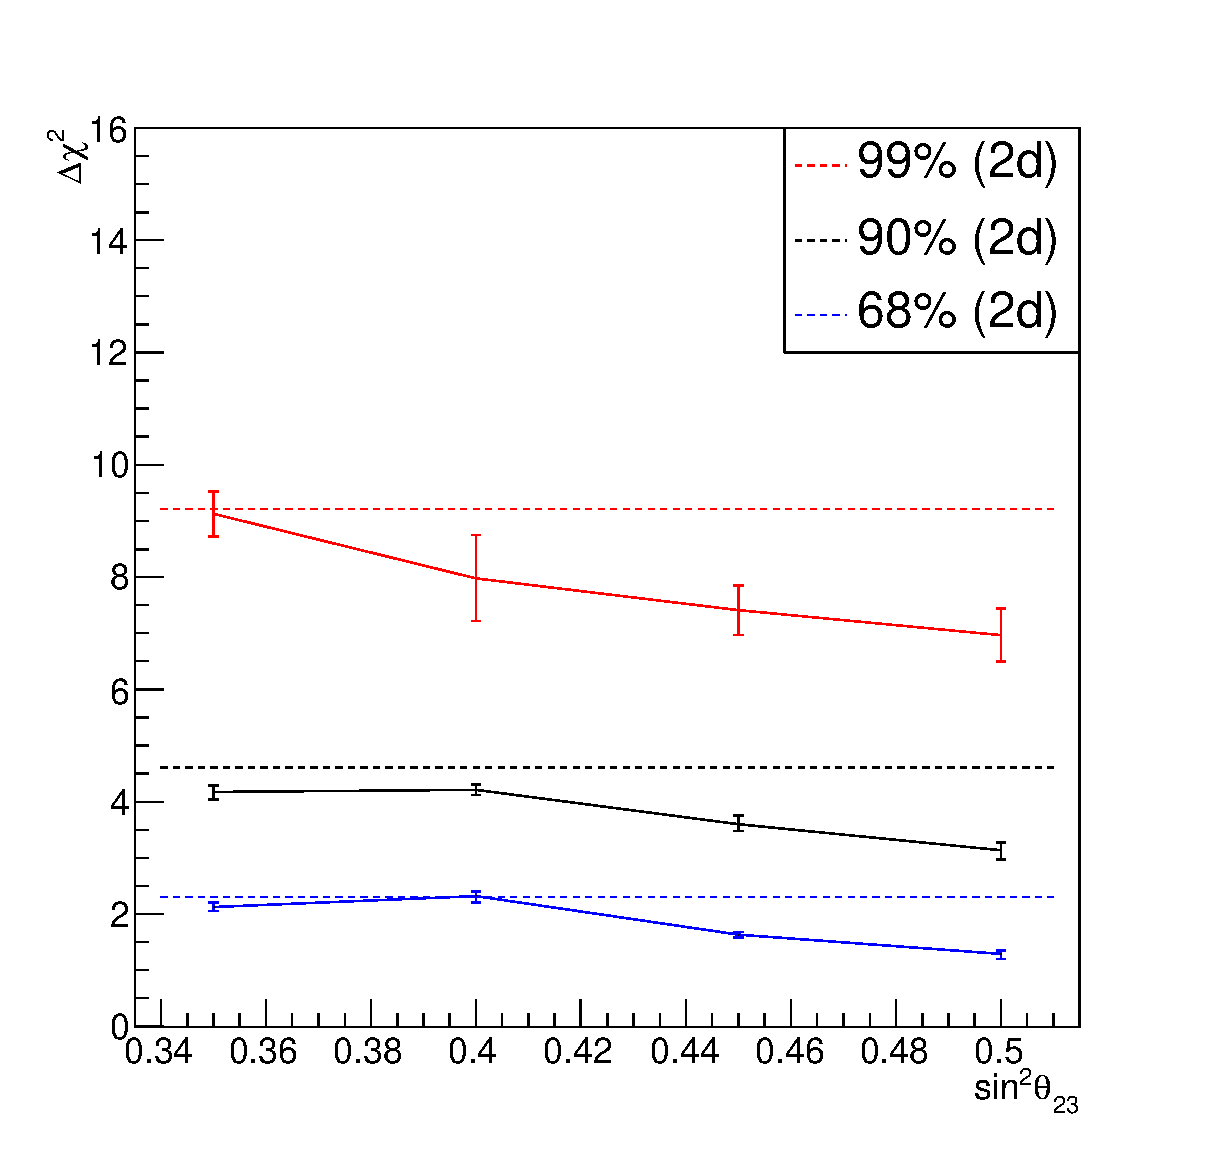
\includegraphics[width=14pc]{./images/appendix/coverage/coverage_study_2D_theta23_dm23sq_stats_osc_all.eps}
\caption {
   Summary of the values of $\Delta\chi^{2}$ at 99\%, 90\% and 68\% confidence intervals in the 2D parameter space ($sin^{2}\theta_{23}$,$|\Delta m^{2}|$) vs the value of $sin^{2}\theta_{23}$ with statistical fluctuations only and fitting $sin^{2}\theta_{13}$ and $\delta_{CP}$. 
True input values for the other oscillation parameters:
$|\Delta m^{2}| = 2.36 \times 10^{-3}$,
  $sin^{2}\theta_{13} = 0.025$ and
        $\delta_{CP}$   = 0.
	}
\label{fig:cov_2D_theta23_dmsq_stats_osc_all}
\end{minipage}
\hspace{0.03\linewidth}
\begin{minipage}[t]{0.46\linewidth}
\center
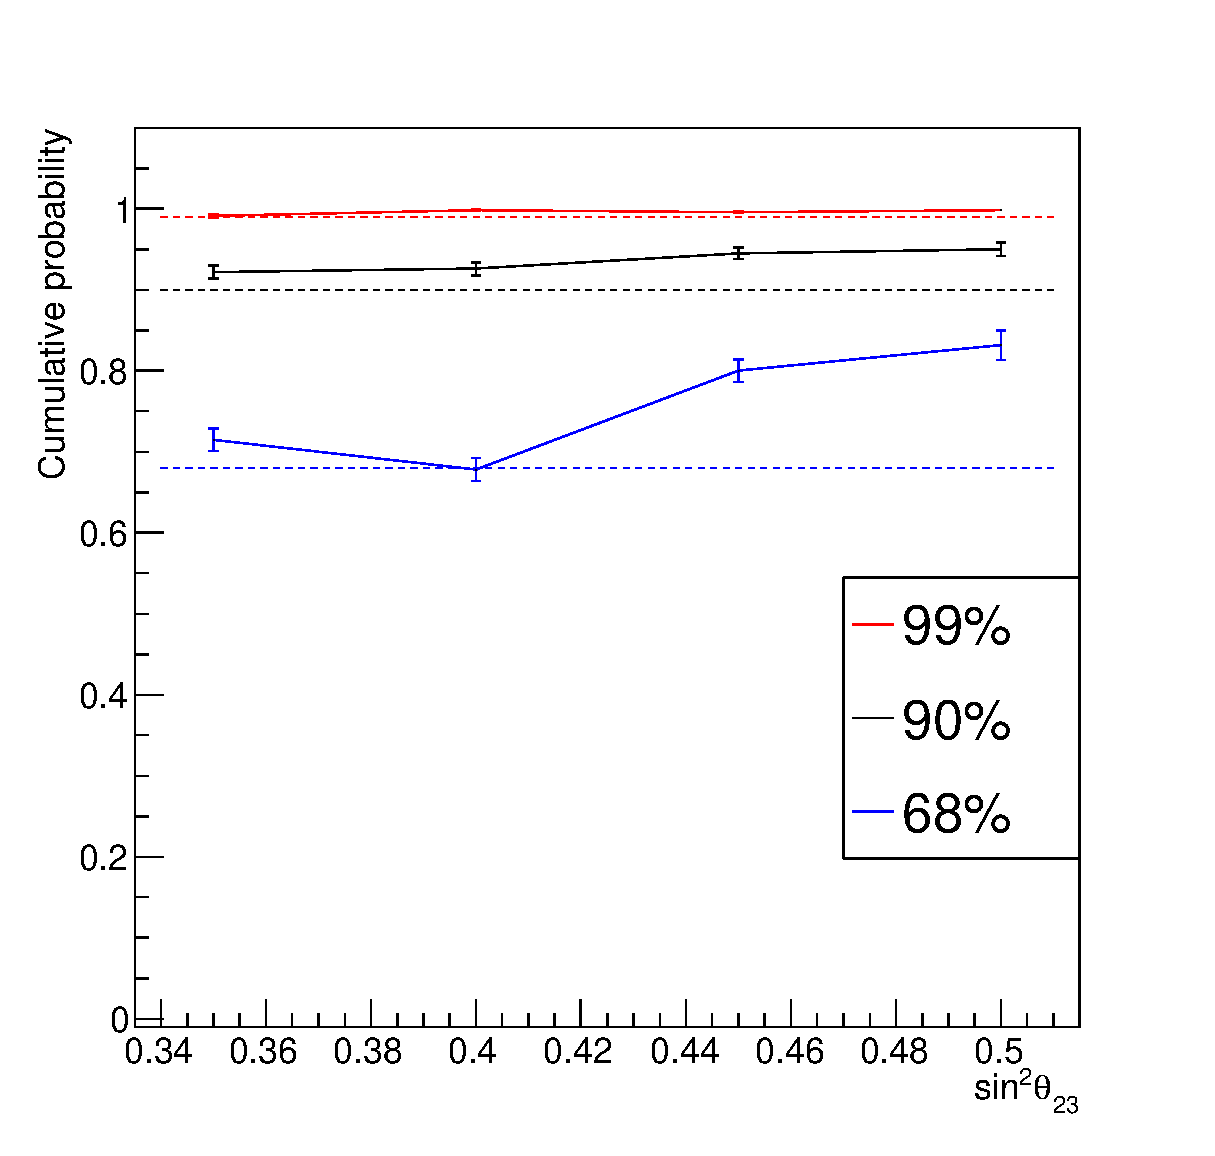
\includegraphics[width=14pc]{./images/appendix/coverage/coverage_study_2D_stats_osc_theta23_dmsq_new_all.eps}
\caption {
   Summary of the values of cumulative probability  for $\Delta\chi^{2}=9.21$ (canonical value for 99\%), $\Delta\chi^{2}=4.61$ (canonical value for 90\%) and $\Delta\chi^{2}=2.30$ (canonical value for 68\%) in the 2D parameter space ($sin^{2}\theta_{23}$,$|\Delta m^{2}|$) vs the value of $sin^{2}\theta_{23}$ with statistical fluctuations only and fitting $sin^{2}\theta_{13}$ and $\delta_{CP}$. 
True input values for the other oscillation parameters:
$|\Delta m^{2}| = 2.36 \times 10^{-3}$,
  $sin^{2}\theta_{13} = 0.025$ and
        $\delta_{CP}$   = 0.
	}
\label{fig:prob_2D_theta23_dmsq_stats_osc_all}
\end{minipage}
\vfill
 \vspace*{0.7cm}
\begin{minipage}[t]{0.46\linewidth}
\center
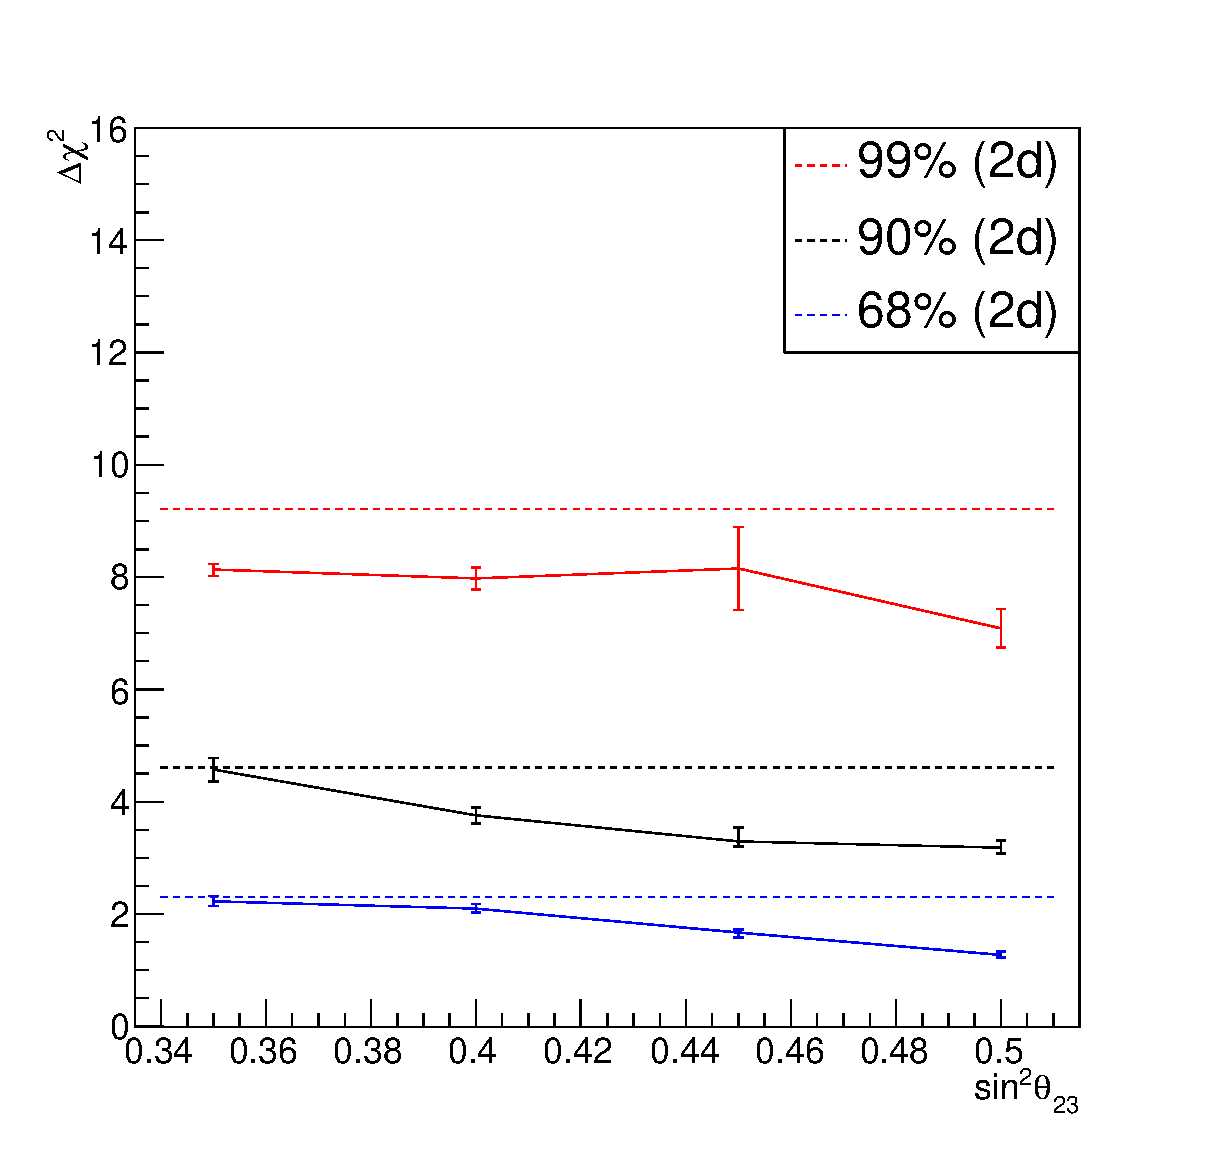
\includegraphics[width=14pc]{./images/appendix/coverage/coverage_study_2D_theta23_dm23sq_syst_osc_all.eps}
\caption {
   Summary of the values of $\Delta\chi^{2}$ at 99\%, 90\% and 68\% confidence intervals in the 2D parameter space ($sin^{2}\theta_{23}$,$|\Delta m^{2}|$) vs the value of $sin^{2}\theta_{23}$ with statistical fluctuations and systematic variations and fitting $sin^{2}\theta_{13}$ and $\delta_{CP}$.
True input values for the other oscillation parameters:
$|\Delta m^{2}| = 2.36 \times 10^{-3}$,
  $sin^{2}\theta_{13} = 0.025$ and
        $\delta_{CP}$   = 0.
	}
\label{fig:cov_2D_theta23_dmsq_syst_osc_all}
\end{minipage}
\hspace{0.03\linewidth}
\begin{minipage}[t]{0.46\linewidth}
\center
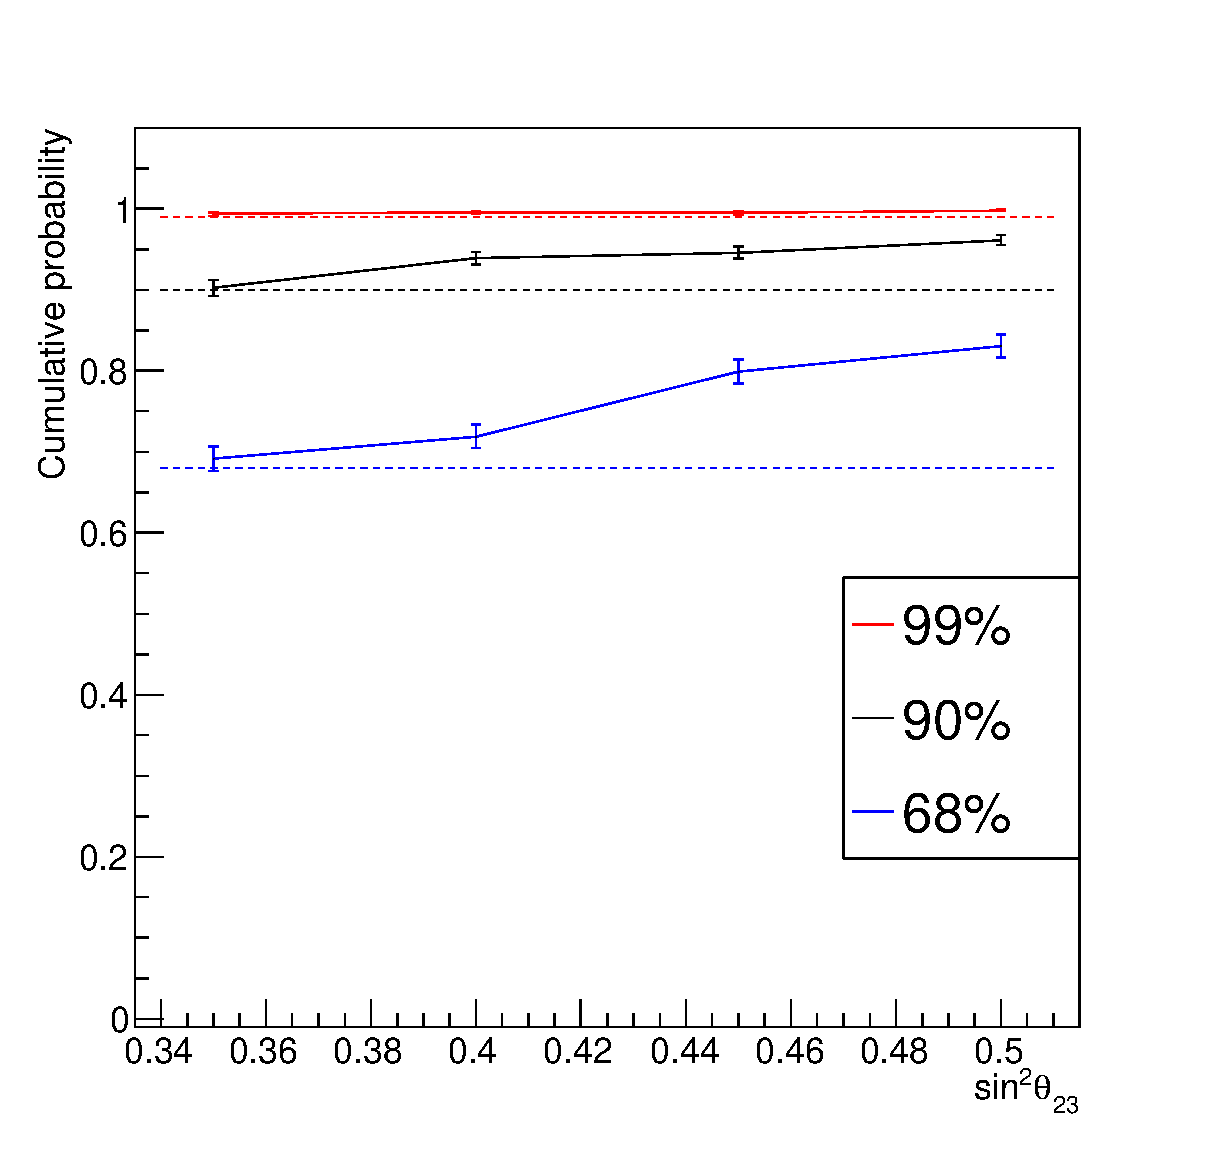
\includegraphics[width=14pc]{./images/appendix/coverage/coverage_study_2D_syst_osc_theta23_dmsq_new_all.eps}
\caption {
   Summary of the values of cumulative probability  for $\Delta\chi^{2}=9.21$ (canonical value for 99\%), $\Delta\chi^{2}=4.61$ (canonical value for 90\%) and $\Delta\chi^{2}=2.30$ (canonical value for 68\%) in the 2D parameter space ($sin^{2}\theta_{23}$,$|\Delta m^{2}|$) vs the value of $sin^{2}\theta_{23}$ with statistical fluctuations and systematic variations and fitting $sin^{2}\theta_{13}$ and $\delta_{CP}$. 
True input values for the other oscillation parameters:
$|\Delta m^{2}| = 2.36 \times 10^{-3}$,
  $sin^{2}\theta_{13} = 0.025$ and
        $\delta_{CP}$   = 0.
	}
\label{fig:prob_2D_theta23_dmsq_syst_osc_all}
\end{minipage}
\end{figure*}
\end{center}


\begin{center}
\begin{figure*}[htb]
\begin{minipage}[t]{0.46\linewidth}
\center
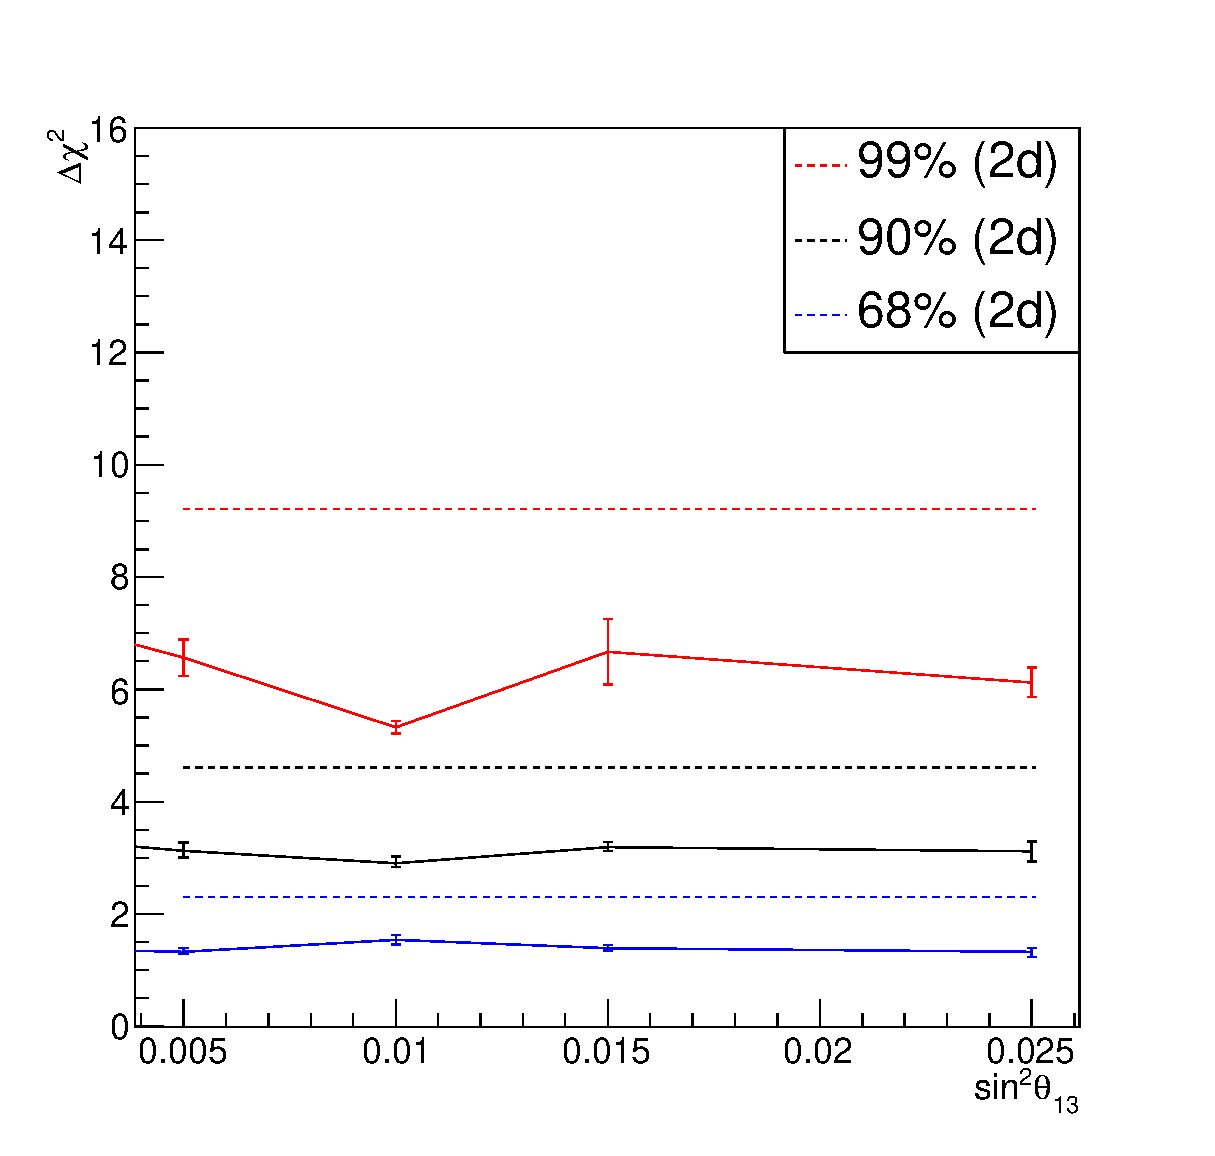
\includegraphics[width=14pc]{./images/appendix/coverage/coverage_study_2D_theta13_dm23sq_stats_osc_all.eps}
\caption {
   Summary of the values of $\Delta\chi^{2}$ at 99\%, 90\% and 68\% confidence intervals in the 2D parameter space ($sin^{2}\theta_{13}$,$|\Delta m^{2}|$) vs the value of $sin^{2}\theta_{13}$ with statistical fluctuations only and fitting $sin^{2}\theta_{23}$ and $\delta_{CP}$.
True input values for the other oscillation parameters:
$|\Delta m^{2}| = 2.36 \times 10^{-3}$,
  $sin^{2}\theta_{23} = 0.5$ and
        $\delta_{CP}$   = 0.
	}
\label{fig:cov_2D_theta13_dmsq_stats_osc_all}
\end{minipage}
\hspace{0.03\linewidth}
\begin{minipage}[t]{0.46\linewidth}
\center
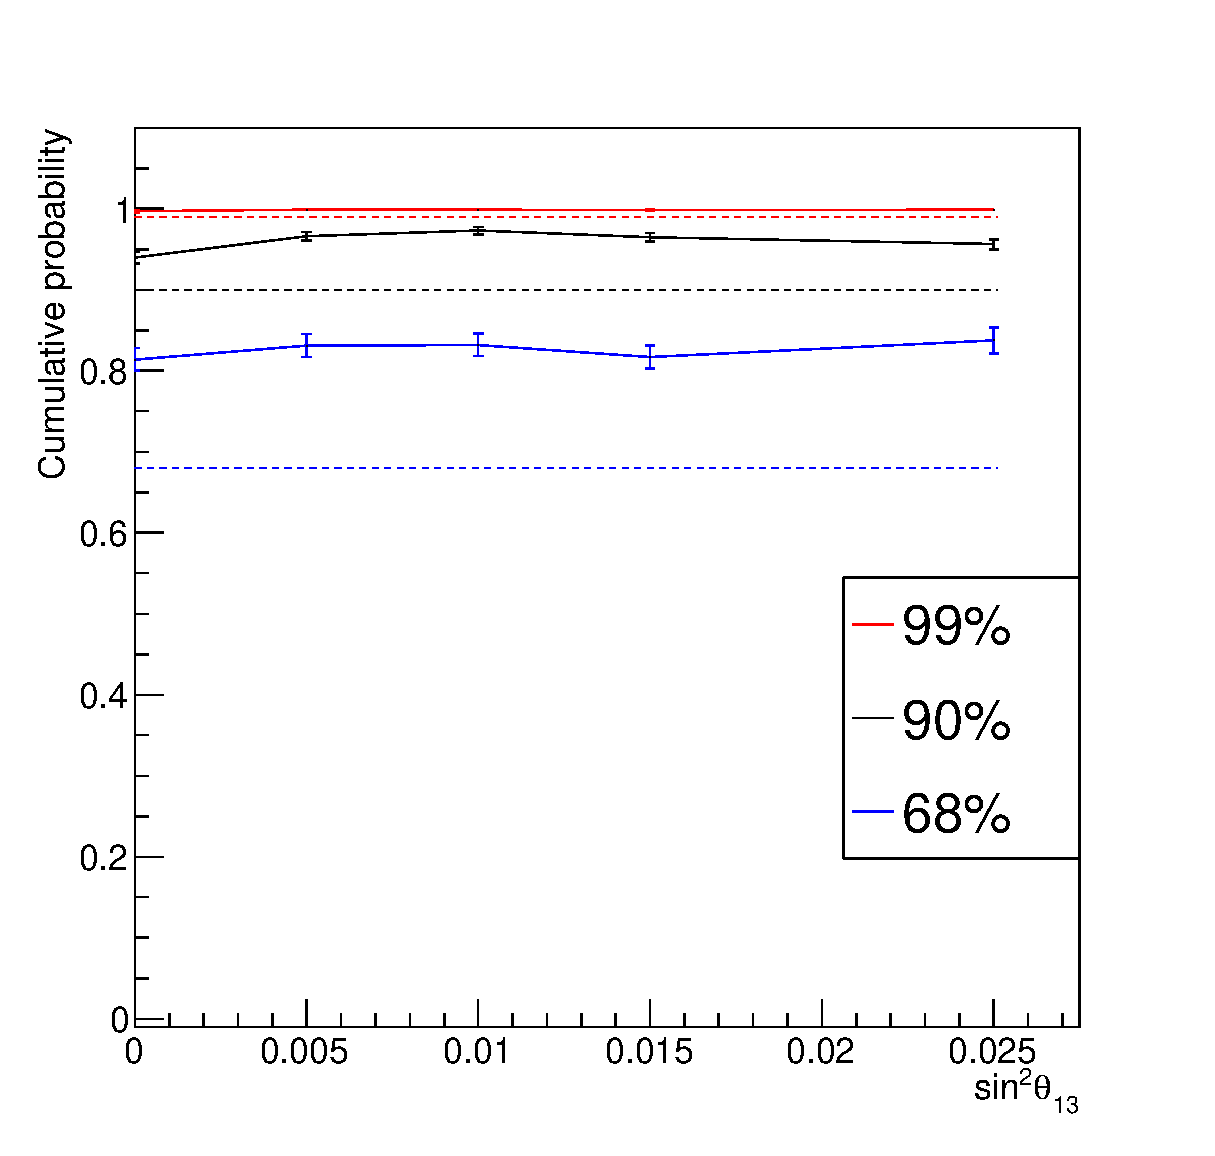
\includegraphics[width=14pc]{./images/appendix/coverage/coverage_study_2D_stats_osc_theta13_dmsq_new_all.eps}
\caption {
   Summary of the values of cumulative probability  for $\Delta\chi^{2}=9.21$ (canonical value for 99\%), $\Delta\chi^{2}=4.61$ (canonical value for 90\%) and $\Delta\chi^{2}=2.30$ (canonical value for 68\%) in the 2D parameter space ($sin^{2}\theta_{13}$,$|\Delta m^{2}|$) vs the value of $sin^{2}\theta_{13}$ with statistical fluctuations only and fitting $sin^{2}\theta_{23}$ and $\delta_{CP}$.
True input values for the other oscillation parameters:
$|\Delta m^{2}| = 2.36 \times 10^{-3}$,
  $sin^{2}\theta_{23} = 0.5$ and
        $\delta_{CP}$   = 0.
	}
\label{fig:prob_2D_theta13_dmsq_stats_osc_all}
\end{minipage}
\vfill
 \vspace*{0.7cm}
\begin{minipage}[t]{0.46\linewidth}
\center
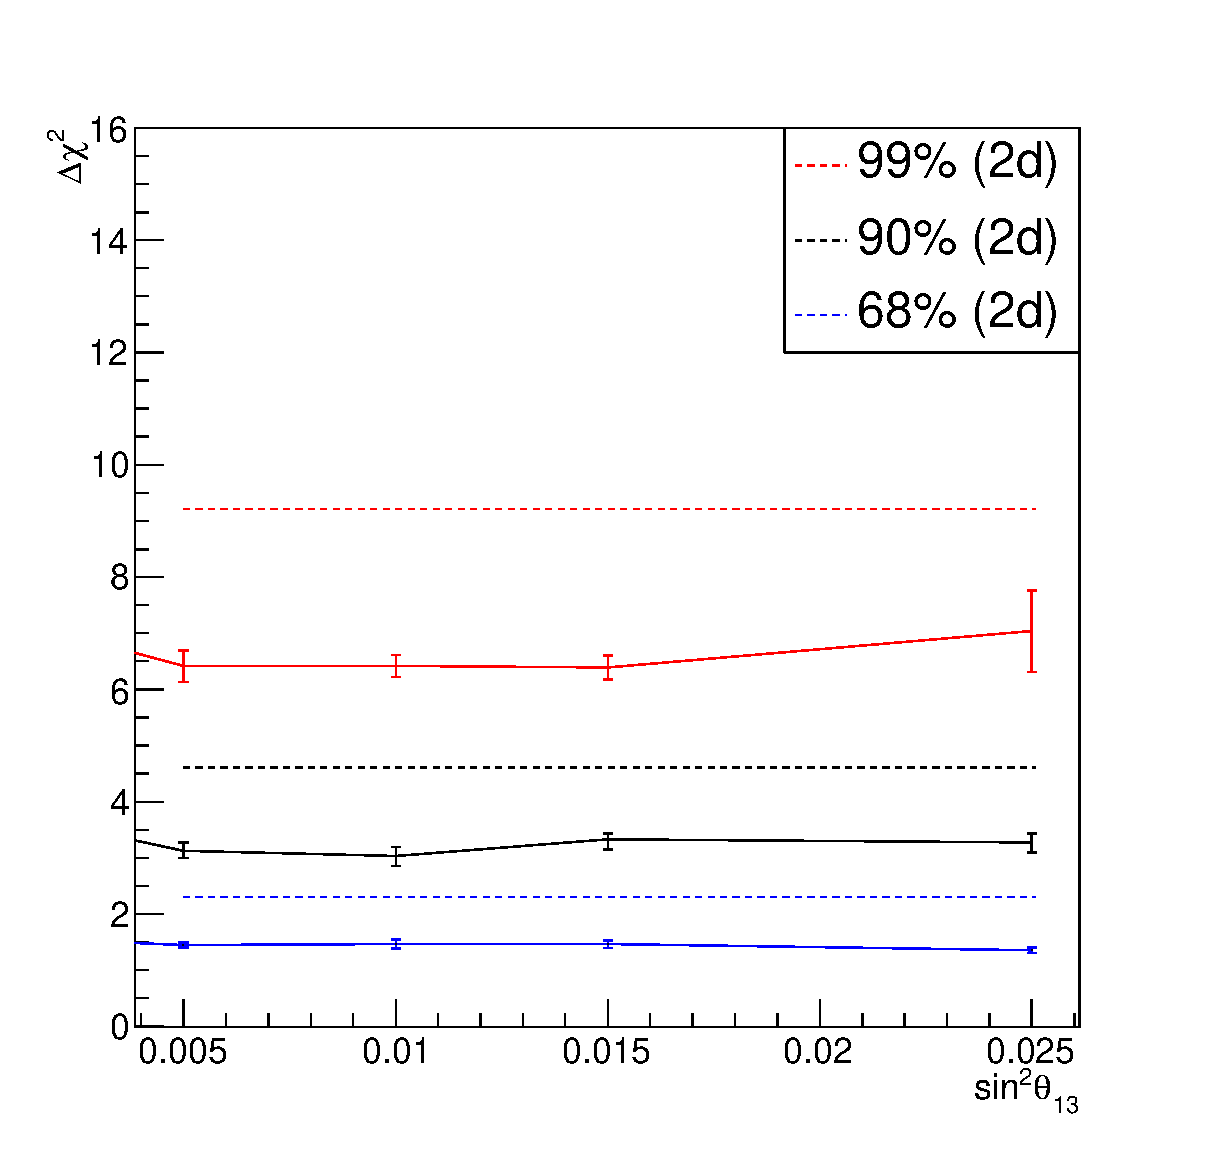
\includegraphics[width=14pc]{./images/appendix/coverage/coverage_study_2D_theta13_dm23sq_syst_osc_all.eps}
\caption {
   Summary of the values of $\Delta\chi^{2}$ at 99\%, 90\% and 68\% confidence intervals  in the 2D parameter space ($sin^{2}\theta_{13}$,$|\Delta m^{2}|$) vs the value of $sin^{2}\theta_{13}$ with statistical fluctuations and systematic variations and fitting $sin^{2}\theta_{23}$ and $\delta_{CP}$.
True input values for the other oscillation parameters:
$|\Delta m^{2}| = 2.36 \times 10^{-3}$,
  $sin^{2}\theta_{23} = 0.5$ and
        $\delta_{CP}$   = 0.
	}
\label{fig:cov_2D_theta13_dmsq_syst_osc_all}
\end{minipage}
\hspace{0.03\linewidth}
\begin{minipage}[t]{0.46\linewidth}
\center
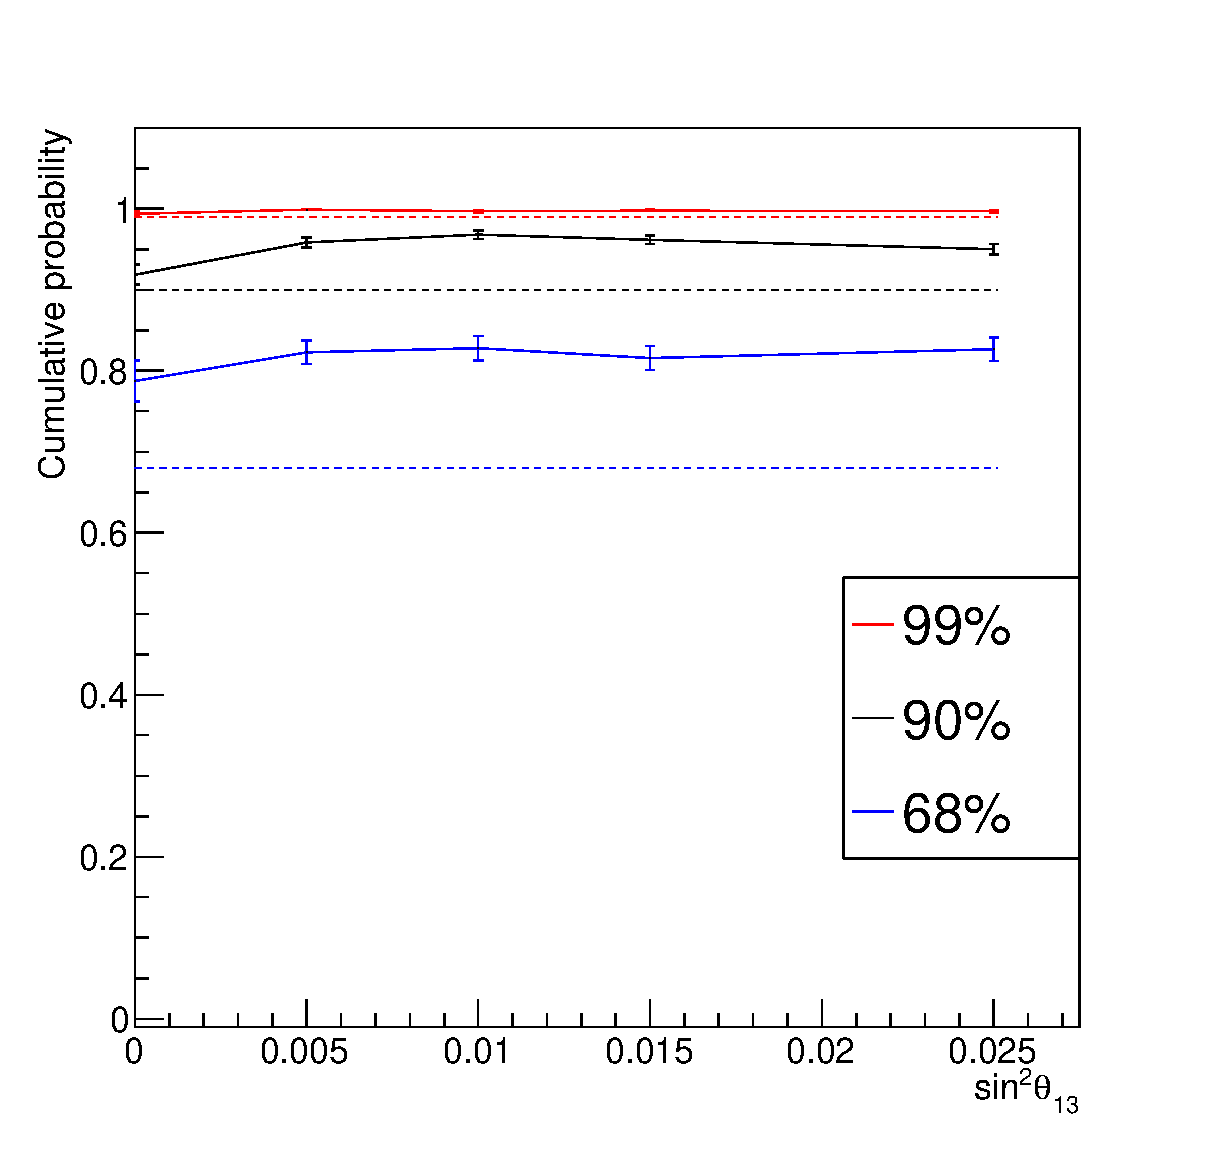
\includegraphics[width=14pc]{./images/appendix/coverage/coverage_study_2D_syst_osc_theta13_dmsq_new_all.eps}
\caption {
   Summary of the values of cumulative probability  for$\Delta\chi^{2}=9.21$ (canonical value for 99\%), $\Delta\chi^{2}=4.61$ (canonical value for 90\%) and $\Delta\chi^{2}=2.30$ (canonical value for 68\%) in the 2D parameter space ($sin^{2}\theta_{13}$,$|\Delta m^{2}|$) vs the value of $sin^{2}\theta_{13}$ with statistical fluctuations and systematic variations and fitting $sin^{2}\theta_{23}$ and $\delta_{CP}$.
True input values for the other oscillation parameters:
$|\Delta m^{2}| = 2.36 \times 10^{-3}$,
  $sin^{2}\theta_{23} = 0.5$ and
        $\delta_{CP}$   = 0.
	}
\label{fig:prob_2D_theta13_dmsq_syst_osc_all}
\end{minipage}
\end{figure*}
\end{center}


\begin{center}
\begin{figure*}[htb]
\begin{minipage}[t]{0.46\linewidth}
\center
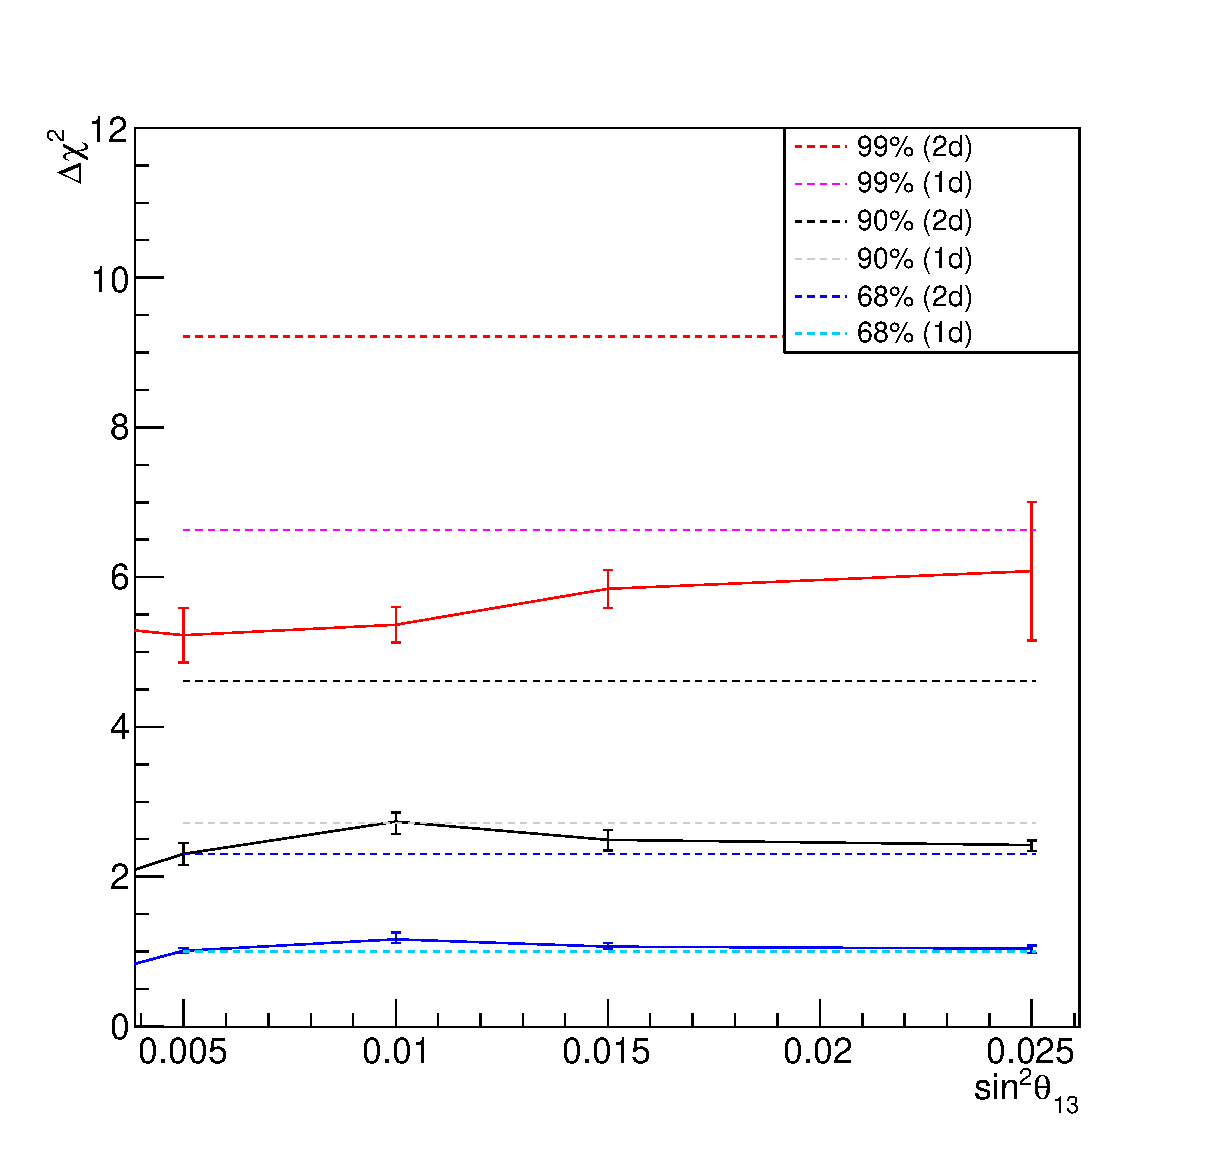
\includegraphics[width=14pc]{./images/appendix/coverage/coverage_study_2D_theta13_deltacp_stats_osc_all.eps}
\caption {
   Summary of the values of $\Delta\chi^{2}$ at 99\%, 90\% and 68\% confidence intervals in the 2D parameter space ($sin^{2}\theta_{13}$,$\delta_{CP}$) vs the value of $sin^{2}\theta_{13}$ with statistical fluctuations only and fitting $sin^{2}\theta_{23}$ and $|\Delta m_{2}|$.
True input values for the other oscillation parameters:
$|\Delta m^{2}| = 2.36 \times 10^{-3}$,
  $sin^{2}\theta_{23} = 0.5$ and
        $\delta_{CP}$   = 0.
	}
\label{fig:cov_2D_theta13_deltacp_stats_osc_all}
\end{minipage} 
\hspace{0.03\linewidth}
\begin{minipage}[t]{0.46\linewidth}
\center
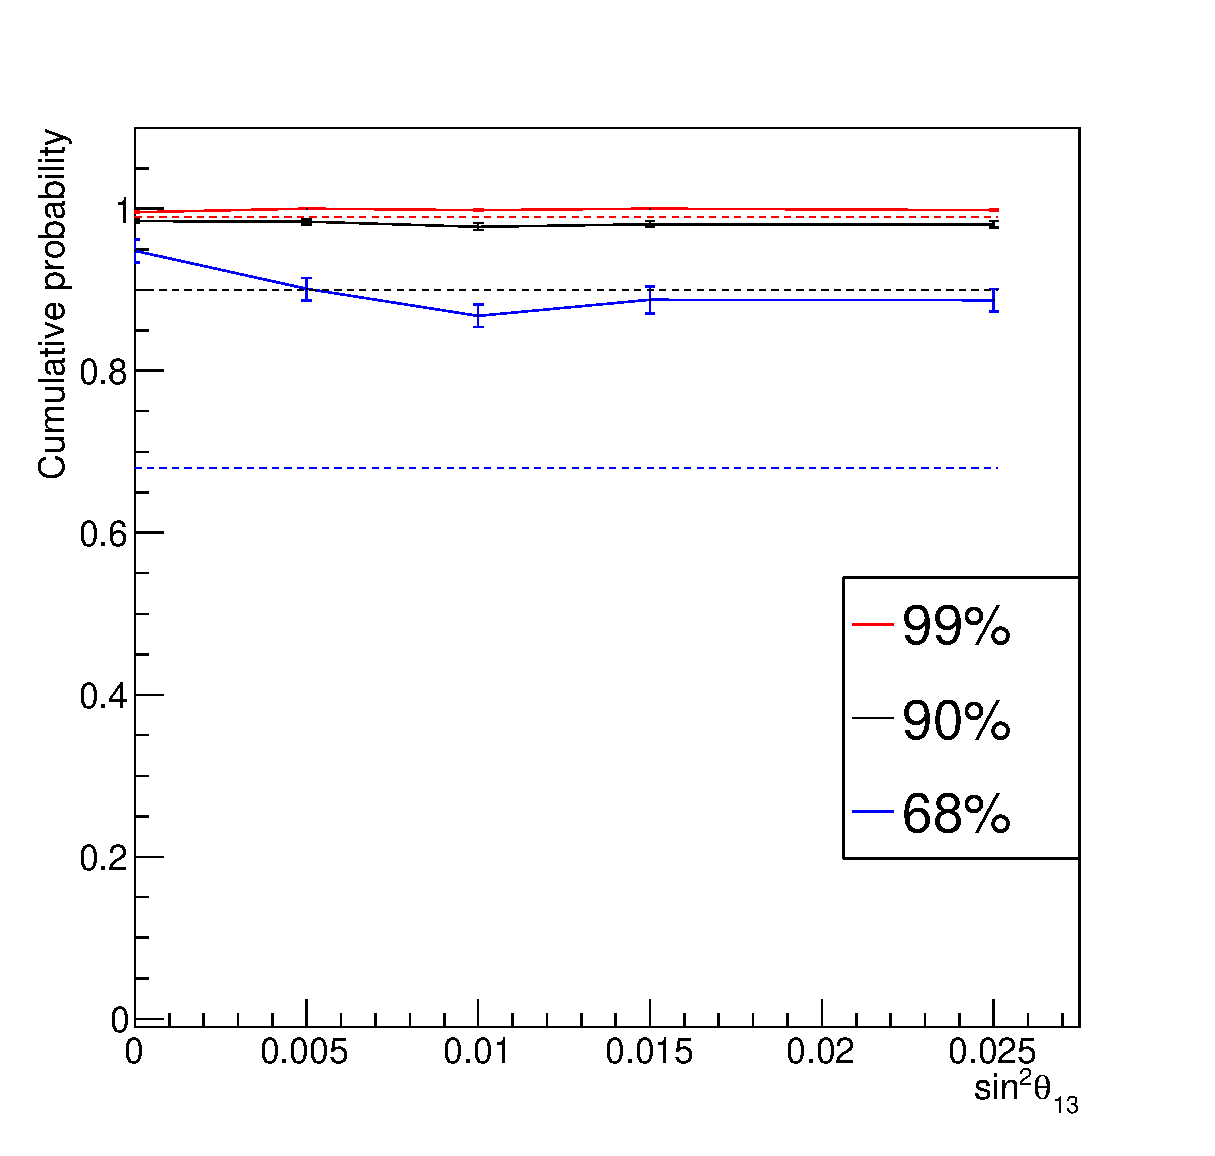
\includegraphics[width=14pc]{./images/appendix/coverage/coverage_study_2D_stats_osc_theta13_deltacp_new_all.eps}
\caption {
   Summary of the values of cumulative probability  for $\Delta\chi^{2}=9.21$ (canonical value for 99\%), $\Delta\chi^{2}=4.61$ (canonical value for 90\%) and $\Delta\chi^{2}=2.30$ (canonical value for 68\%) in the 2D parameter space ($sin^{2}\theta_{13}$,$\delta_{CP}$) vs the value of $sin^{2}\theta_{13}$ with statistical fluctuations only and fitting $sin^{2}\theta_{23}$ and $|\Delta m_{2}|$.
True input values for the other oscillation parameters:
$|\Delta m^{2}| = 2.36 \times 10^{-3}$,
  $sin^{2}\theta_{23} = 0.5$ and
        $\delta_{CP}$   = 0.
	}
\label{fig:prob_2D_theta13_deltacp_stats_osc_all}
\end{minipage} 
\vfill
 \vspace*{0.7cm}
\begin{minipage}[t]{0.46\linewidth}
\center
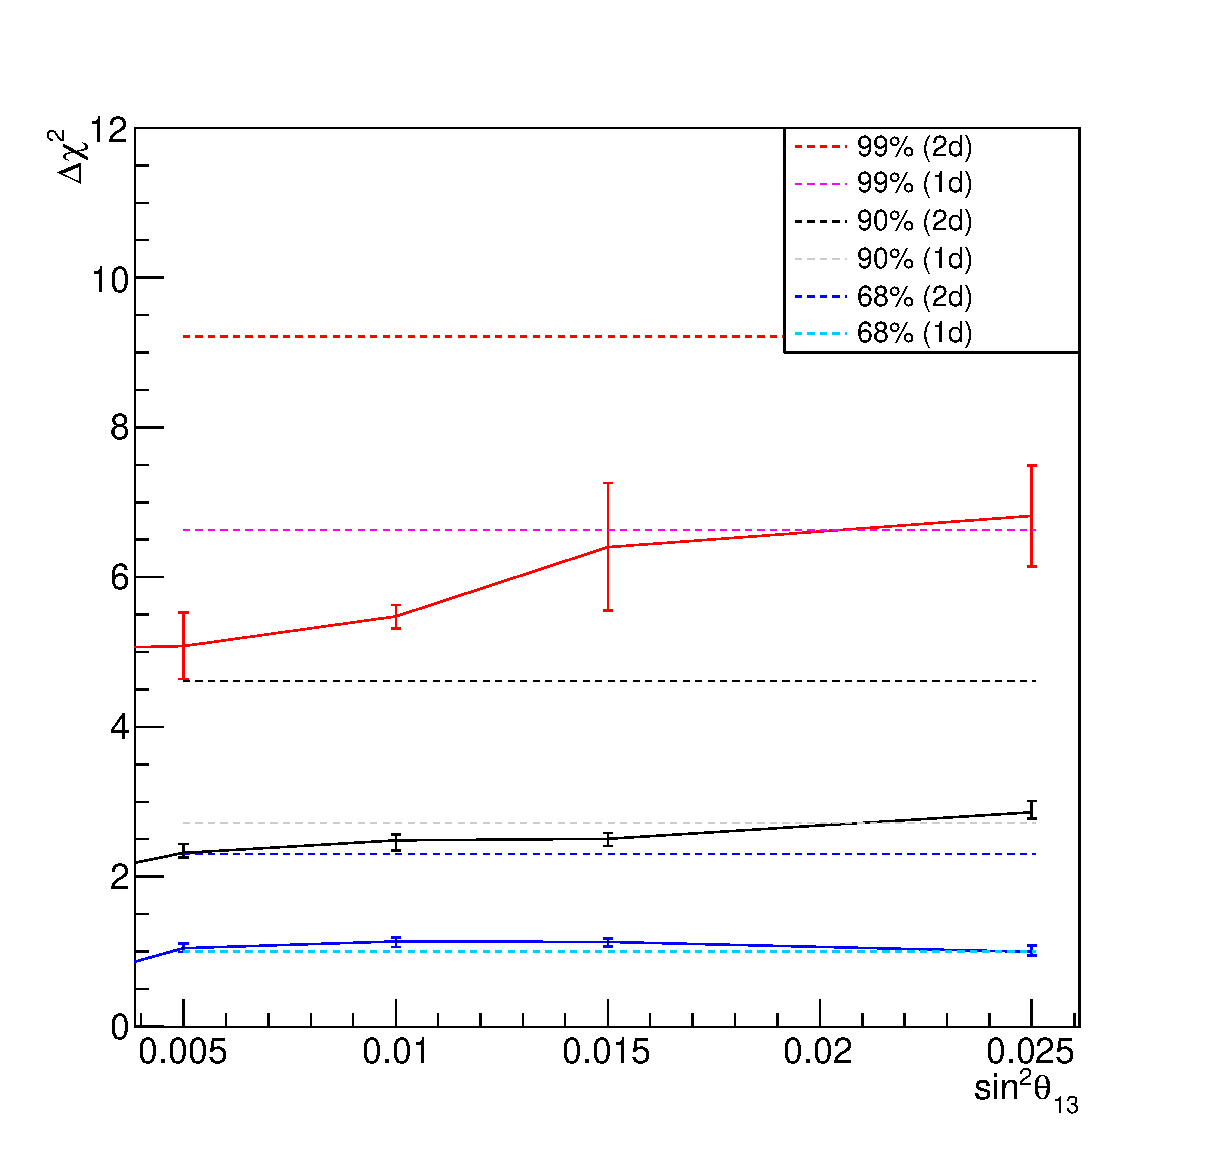
\includegraphics[width=14pc]{./images/appendix/coverage/coverage_study_2D_theta13_deltacp_syst_osc_all.eps}
\caption {
   Summary of the values of $\Delta\chi^{2}$ at 99\%, 90\% and 68\% confidence intervals in the 2D parameter space ($sin^{2}\theta_{13}$,$\delta_{CP}$) vs the value of $sin^{2}\theta_{13}$ with statistical fluctuations and systematic variations and fitting $sin^{2}\theta_{23}$ and $|\Delta m_{2}|$.
True input values for the other oscillation parameters:
$|\Delta m^{2}| = 2.36 \times 10^{-3}$,
  $sin^{2}\theta_{23} = 0.5$ and
        $\delta_{CP}$   = 0.
	}
\label{fig:cov_2D_theta13_deltacp_syst_osc_all}
\end{minipage} 
\hspace{0.03\linewidth}
\begin{minipage}[t]{0.46\linewidth}
\center
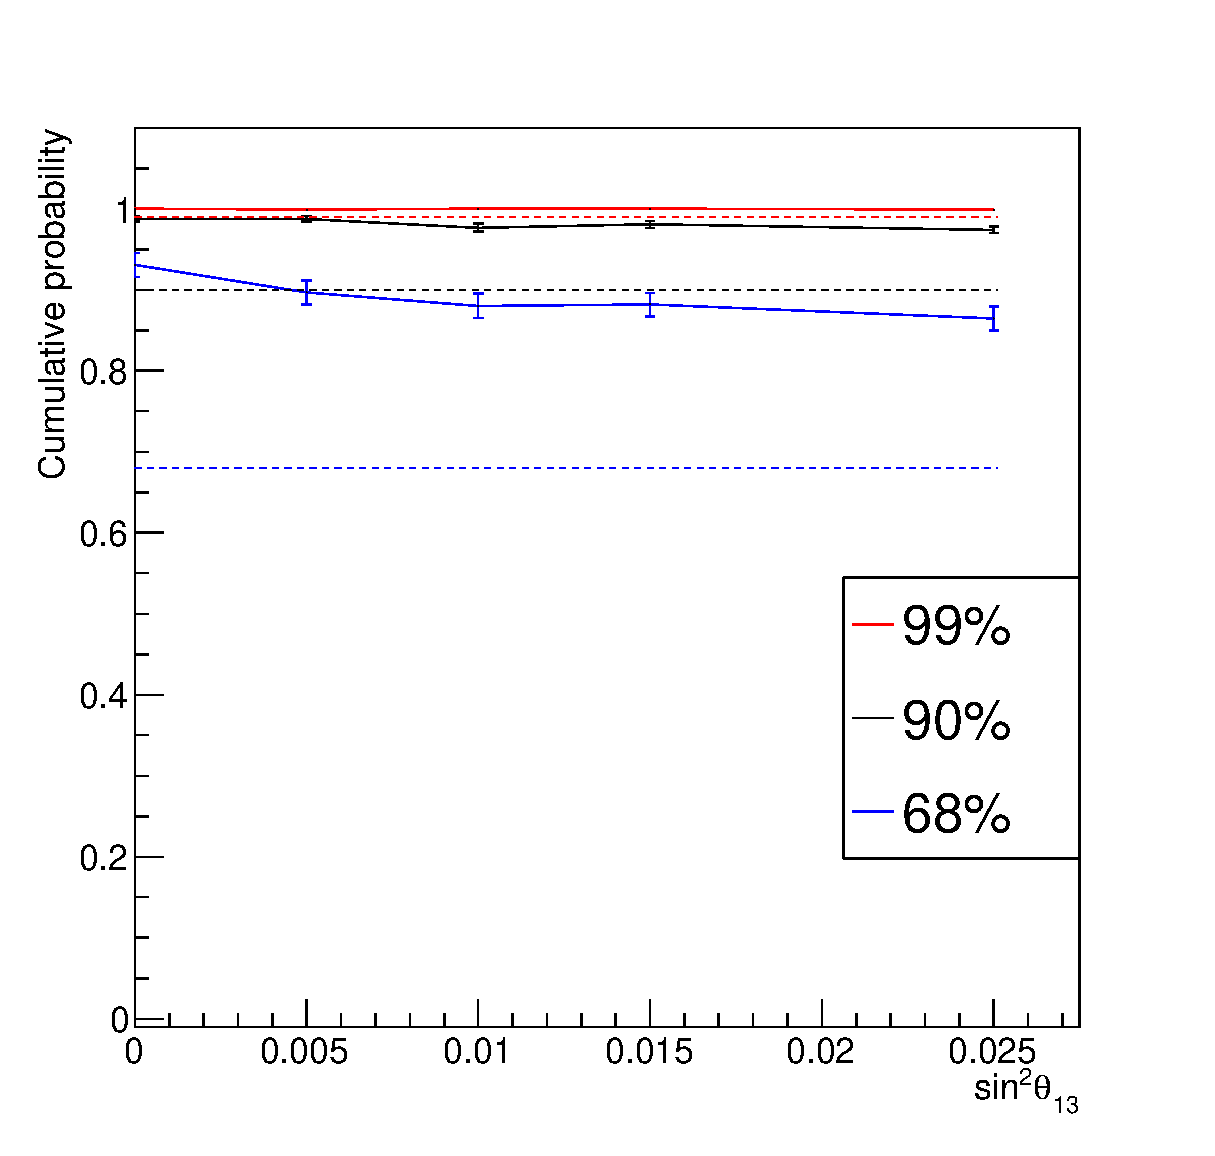
\includegraphics[width=14pc]{./images/appendix/coverage/coverage_study_2D_syst_osc_theta13_deltacp_new_all.eps}
\caption {
   Summary of the values of cumulative probability  for $\Delta\chi^{2}=9.21$ (canonical value for 99\%), $\Delta\chi^{2}=4.61$ (canonical value for 90\%) and $\Delta\chi^{2}=2.30$ (canonical value for 68\%) in the 2D parameter space ($sin^{2}\theta_{13}$,$\delta_{CP}$) vs the value of $sin^{2}\theta_{13}$ with statistical fluctuations and systematic variations and fitting $sin^{2}\theta_{23}$ and $|\Delta m_{2}|$.
True input values for the other oscillation parameters:
$|\Delta m^{2}| = 2.36 \times 10^{-3}$,
  $sin^{2}\theta_{23} = 0.5$ and
        $\delta_{CP}$   = 0.
	}
\label{fig:prob_2D_theta13_deltacp_syst_osc_all}
\end{minipage} 
\end{figure*}
\end{center}



%% FIGURES FOR 2D theta13-dmsq

%\begin{center}
%\begin{figure*}[htb]
%\begin{minipage}[t]{0.46\linewidth}
%\center
%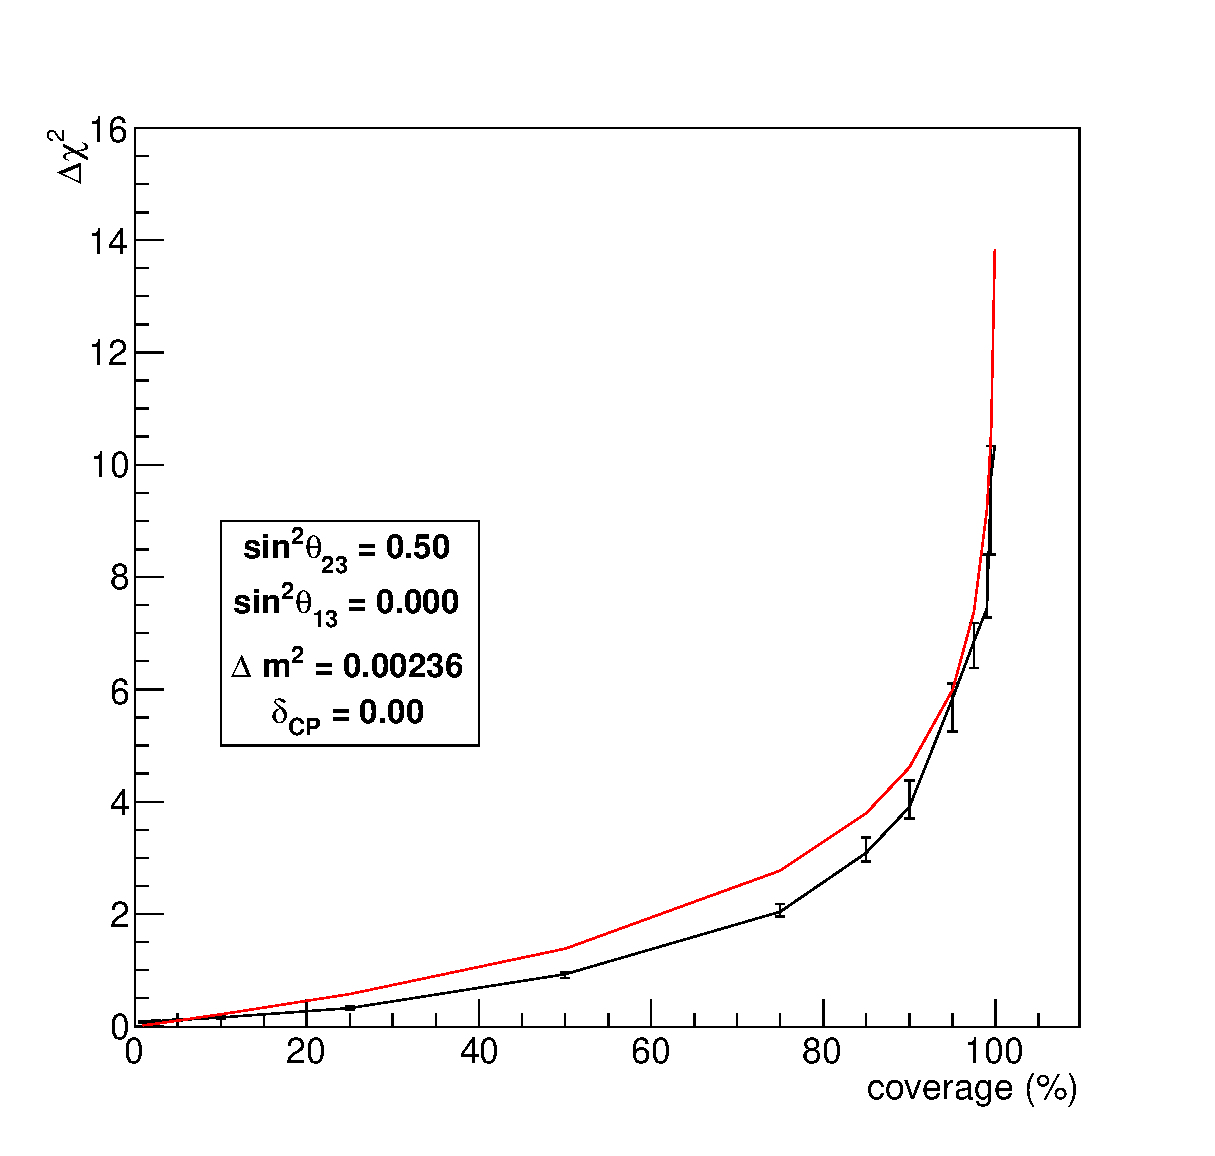
\includegraphics[width=14pc]{./images/appendix/coverage/coverage_study_2D_theta13_dm23sq_syst_osc_0.eps}
%\center
%\caption {
%   Distribution of $\Delta\chi^{2}$ vs coverage in the ($sin^{2}\theta_{13}$,$|\Delta m^{2}|$) parameter space
%  from 1k toy MC experiments generated with the Run 1+2+3 POT
%  with statistical fluctuations and systematic variations at the oscillation point: 
%  $|\Delta m^{2}| = 2.36 \times 10^{-3}$,
%  $sin^{2}\theta_{23} = 0.5$,
%  $sin^{2}\theta_{13} = 0.005$ and
%  	$\delta_{CP}$	= 0.
%	}
%\label{fig:cov_2D_theta13_dm23sq_syst_osc_0}
%\end{minipage}
%\hspace{0.03\linewidth}
%\begin{minipage}[t]{0.46\linewidth}
%\center
%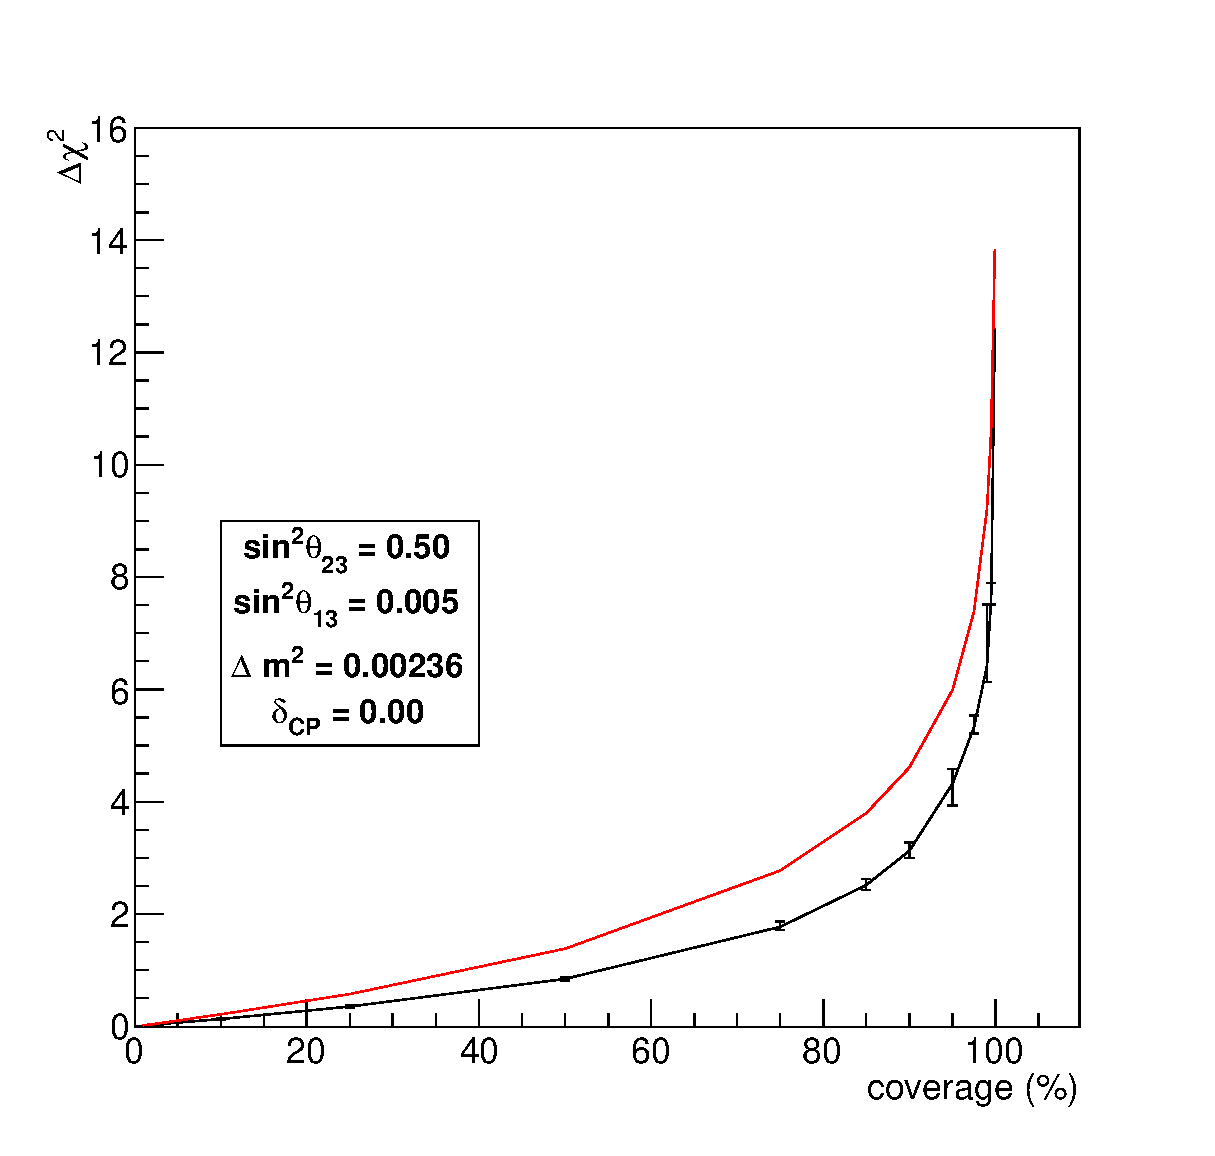
\includegraphics[width=14pc]{./images/appendix/coverage/coverage_study_2D_theta13_dm23sq_syst_osc_1.eps}
%\center
%\caption {
%   Distribution of $\Delta\chi^{2}$ vs coverage in the ($sin^{2}\theta_{13}$,$|\Delta m^{2}|$) parameter space
%  from 1k toy MC experiments generated with the Run 1+2+3 POT
% with statistical fluctuations and systematic variations at the oscillation point: 
%  $|\Delta m^{2}| = 2.36 \times 10^{-3}$,
%  $sin^{2}\theta_{23} = 0.5$,
%  $sin^{2}\theta_{13} = 0.01$ and
%  	$\delta_{CP}$	= 0.
%	}
%\label{fig:cov_2D_theta13_dm23sq_syst_osc_1}
%\end{minipage}
%\vfill
%\vspace*{0.7cm}
%\begin{minipage}[t]{0.46\linewidth}
%\center
%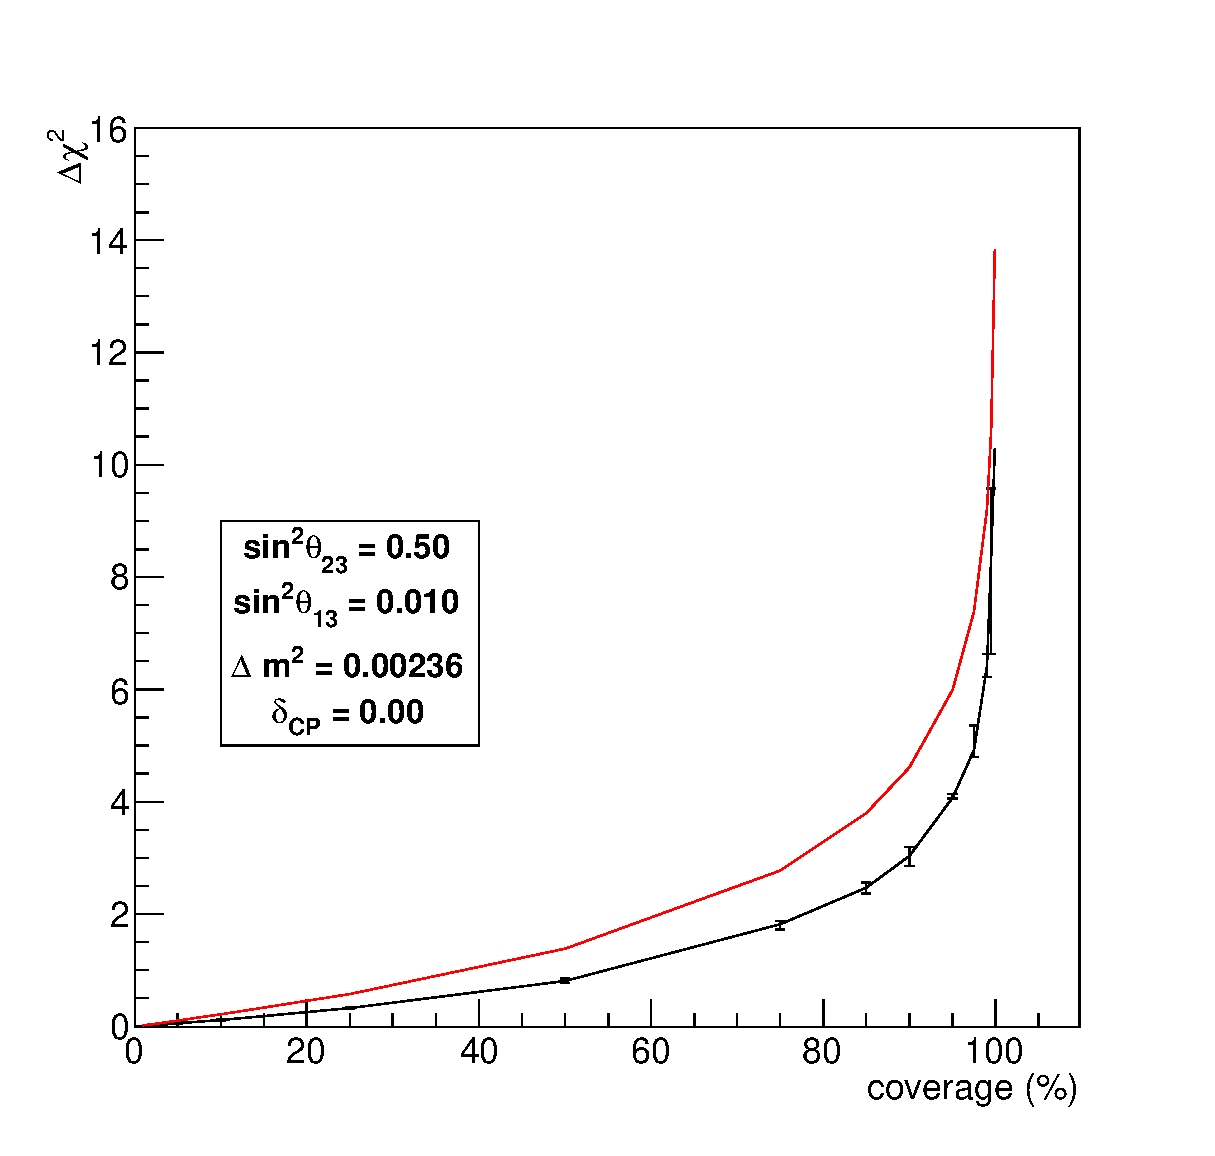
\includegraphics[width=14pc]{./images/appendix/coverage/coverage_study_2D_theta13_dm23sq_syst_osc_2.eps}
%\center
%\caption {
%   Distribution of $\Delta\chi^{2}$ vs coverage in the ($sin^{2}\theta_{13}$,$|\Delta m^{2}|$) parameter space
%  from 1k toy MC experiments generated with the Run 1+2+3 POT
%   with statistical fluctuations and systematic variations at the oscillation point: 
%  $|\Delta m^{2}| = 2.36 \times 10^{-3}$,
%  $sin^{2}\theta_{23} = 0.5$,
%  $sin^{2}\theta_{13} = 0.015$ and
%  	$\delta_{CP}$	= 0.
%	}
%\label{fig:cov_2D_theta13_dm23sq_syst_osc_2}
%\end{minipage}
%\hspace{0.03\linewidth}
%\begin{minipage}[t]{0.46\linewidth}
%\center
%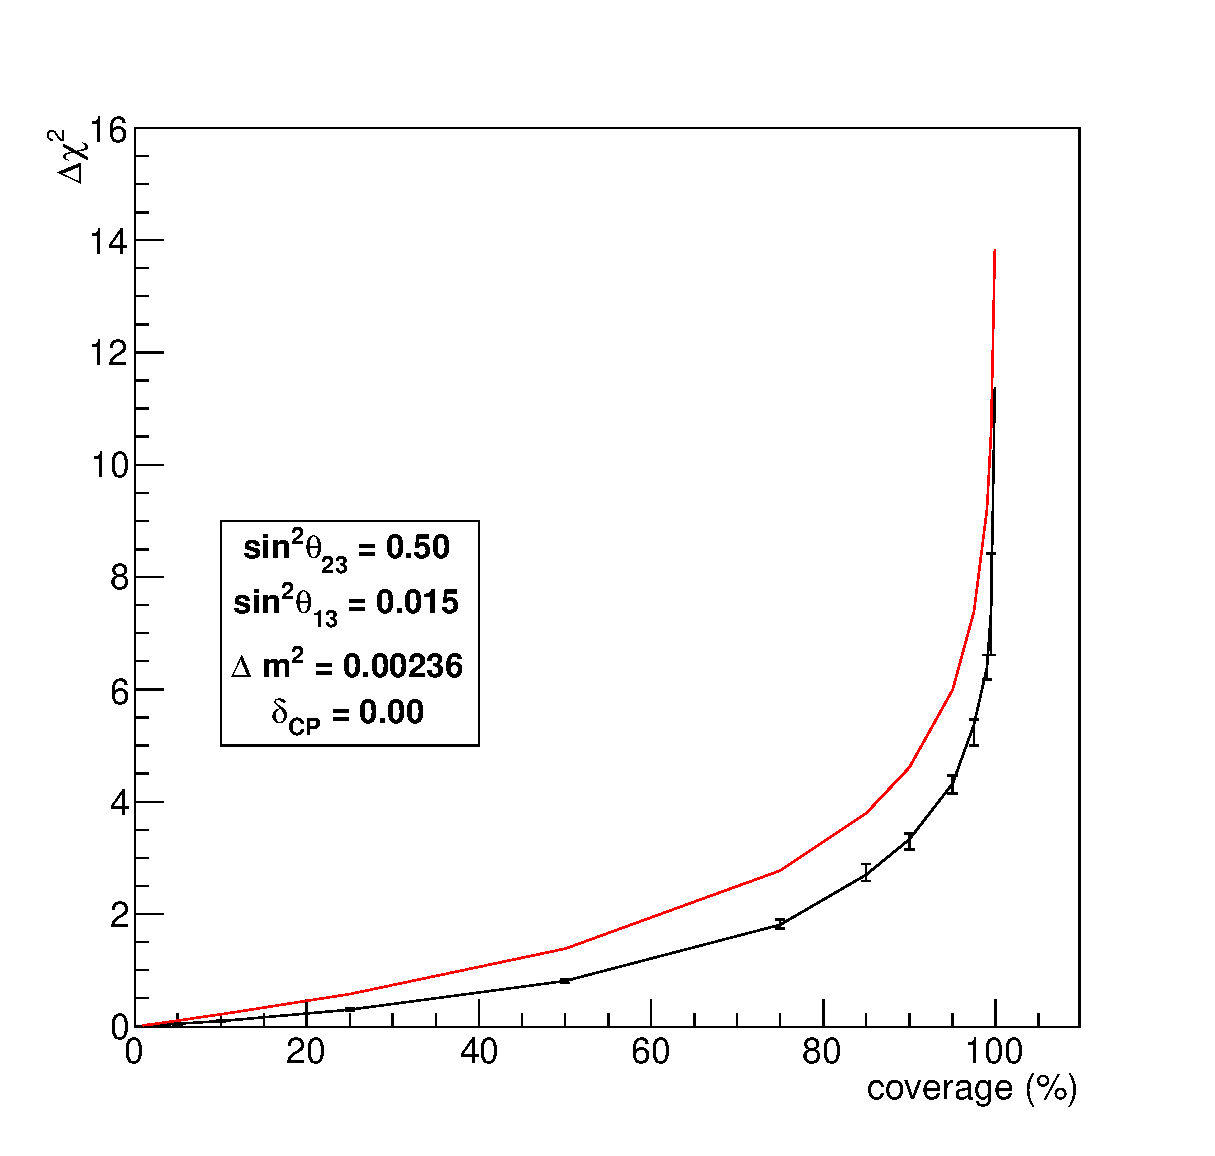
\includegraphics[width=14pc]{./images/appendix/coverage/coverage_study_2D_theta13_dm23sq_syst_osc_3.eps}
%\center
%\caption {
%   Distribution of $\Delta\chi^{2}$ vs coverage in the ($sin^{2}\theta_{13}$,$|\Delta m^{2}|$) parameter space
%  from 1k toy MC experiments generated with the Run 1+2+3 POT
% with statistical fluctuations and systematic variations at the oscillation point: 
%  $|\Delta m^{2}| = 2.36 \times 10^{-3}$,
%  $sin^{2}\theta_{23} = 0.5$,
%  $sin^{2}\theta_{13} = 0.025$ and
%  	$\delta_{CP}$	= 0.
%	}
%\label{fig:cov_2D_theta13_dm23sq_syst_osc_3}
%\end{minipage}
%\vfill
%\vspace*{0.7cm}
%\center
%\begin{minipage}[t]{0.46\linewidth}
%\center
%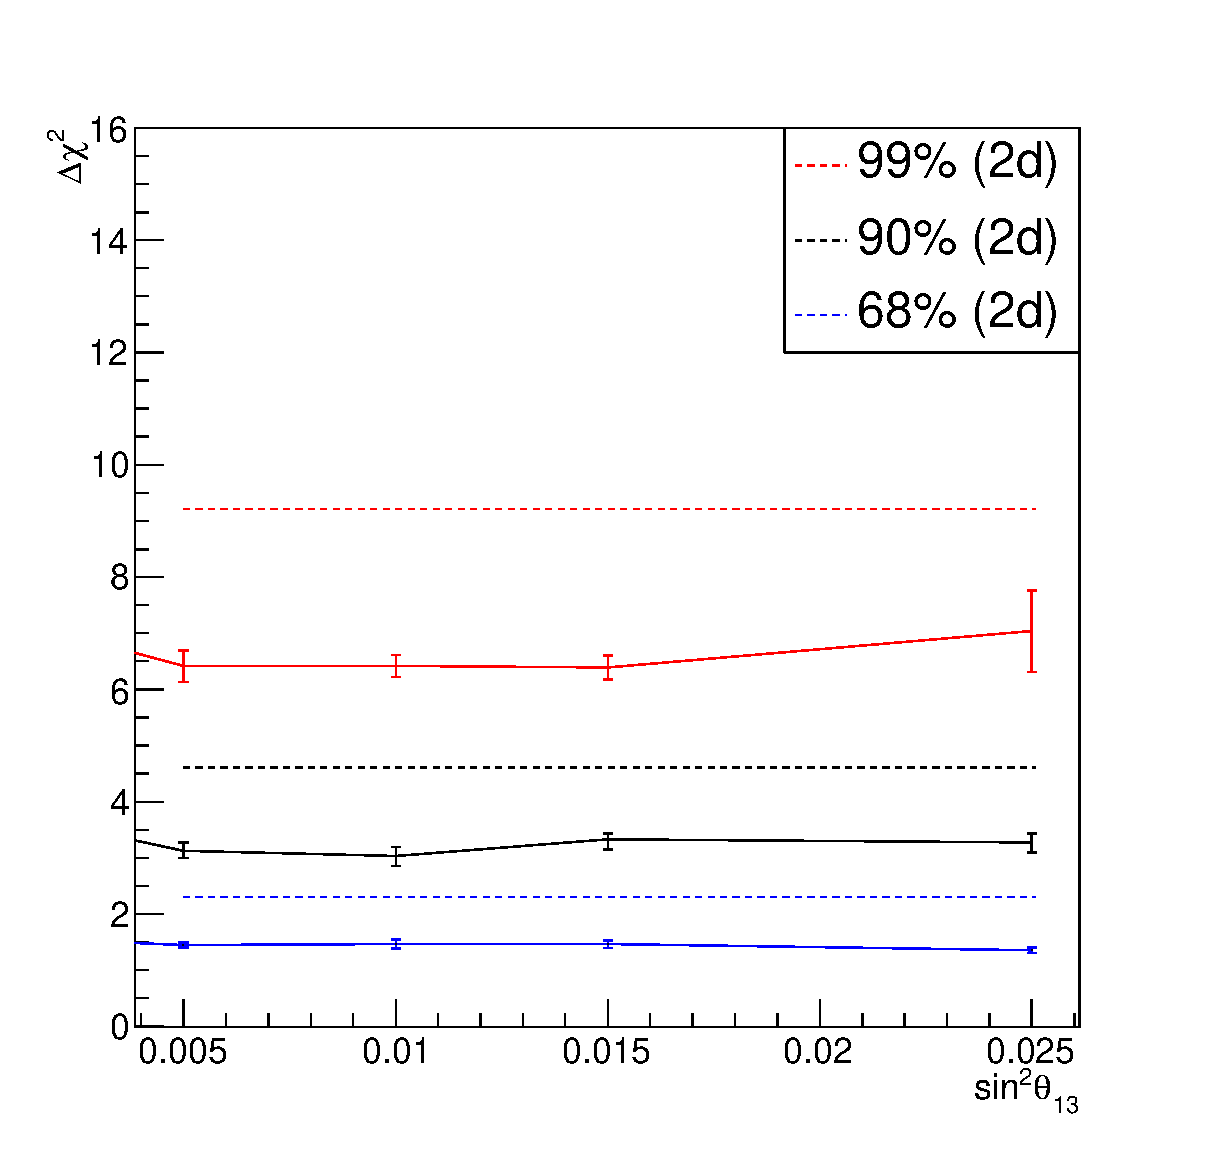
\includegraphics[width=14pc]{./images/appendix/coverage/coverage_study_2D_theta13_dm23sq_syst_osc_all.eps}
%\caption {
%   Summary of figures \ref{fig:cov_2D_theta13_dm23sq_syst_osc_0}-\ref{fig:cov_2D_theta13_dm23sq_syst_osc_3}
%showing the value of $\Delta\chi^{2}$ at 99\%, 90\% and 68\% confidence intervals vs the value of $sin^{2}\theta_{13}$.
%	}
%\label{fig:cov_2D_theta13_dm23sq_syst_osc_all}
%\end{minipage}
%\end{figure*}
%\end{center}


%% FIGURES FOR 2D theta13-dmsq

%\begin{center}
%\begin{figure*}[htb]
%\begin{minipage}[t]{0.46\linewidth}
%\center
%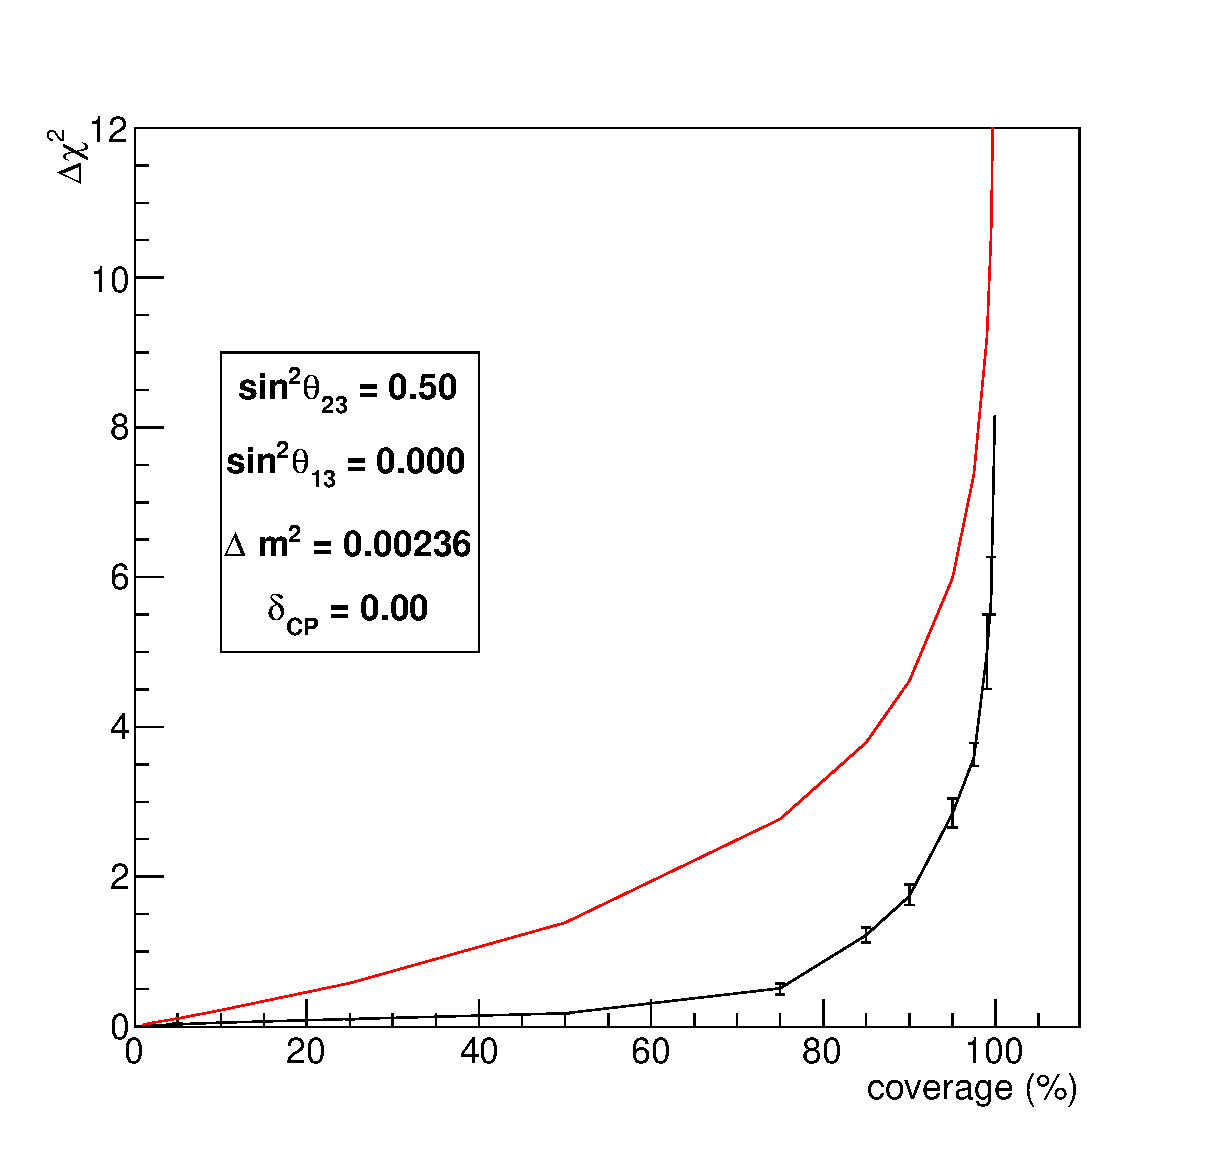
\includegraphics[width=14pc]{./images/appendix/coverage/coverage_study_2D_theta13_deltacp_syst_osc_0.eps}
%\center
%\caption {
%   Distribution of $\Delta\chi^{2}$ vs coverage in the ($sin^{2}\theta_{13}$,$\delta_{CP}$) parameter space
%  from 1k toy MC experiments generated with the Run 1+2+3 POT
% with statistical fluctuations and systematic variations at the oscillation point: 
%  $|\Delta m^{2}| = 2.36 \times 10^{-3}$,
%  $sin^{2}\theta_{23} = 0.5$,
%  $sin^{2}\theta_{13} = 0.005$ and
%  	$\delta_{CP}$	= 0.
%	}
%\label{fig:cov_2D_theta13_deltacp_syst_osc_0}
%\end{minipage}
%\hspace{0.03\linewidth}
%\begin{minipage}[t]{0.46\linewidth}
%\center
%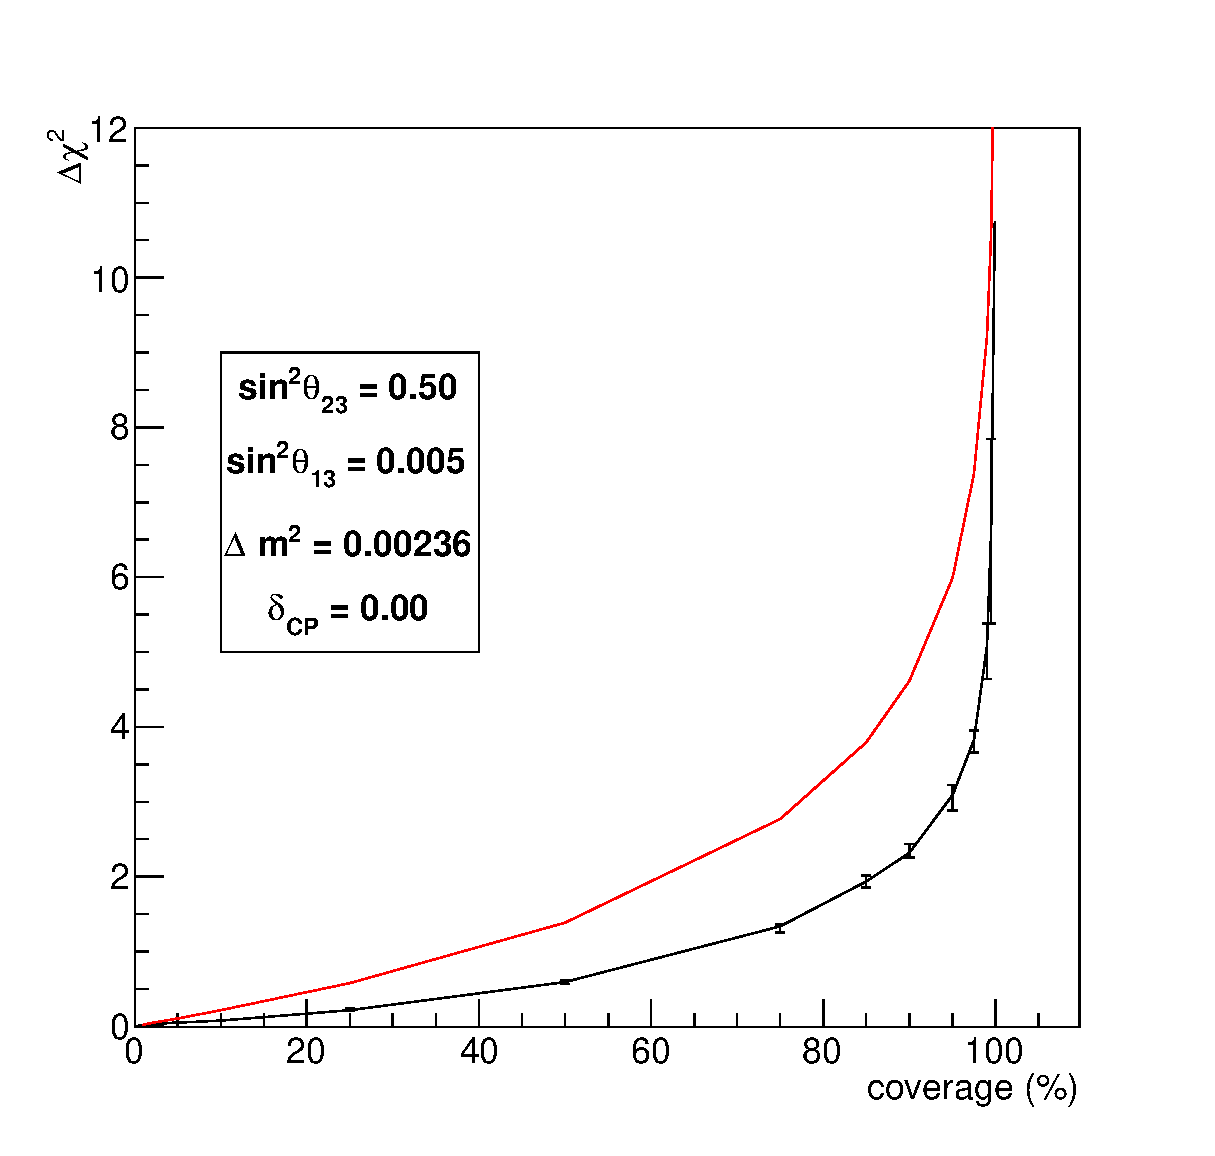
\includegraphics[width=14pc]{./images/appendix/coverage/coverage_study_2D_theta13_deltacp_syst_osc_1.eps}
%\center
%\caption {
%   Distribution of $\Delta\chi^{2}$ vs coverage in the ($sin^{2}\theta_{13}$,$\delta_{CP}$) parameter space
%  from 1k toy MC experiments generated with the Run 1+2+3 POT
% with statistical fluctuations and systematic variations at the oscillation point: 
%  $|\Delta m^{2}| = 2.36 \times 10^{-3}$,
%  $sin^{2}\theta_{23} = 0.5$,
%  $sin^{2}\theta_{13} = 0.01$ and
%  	$\delta_{CP}$	= 0.
%	}
%\label{fig:cov_2D_theta13_deltacp_syst_osc_1}
%\end{minipage}
%\vfill
%\vspace*{0.7cm}
%\begin{minipage}[t]{0.46\linewidth}
%\center
%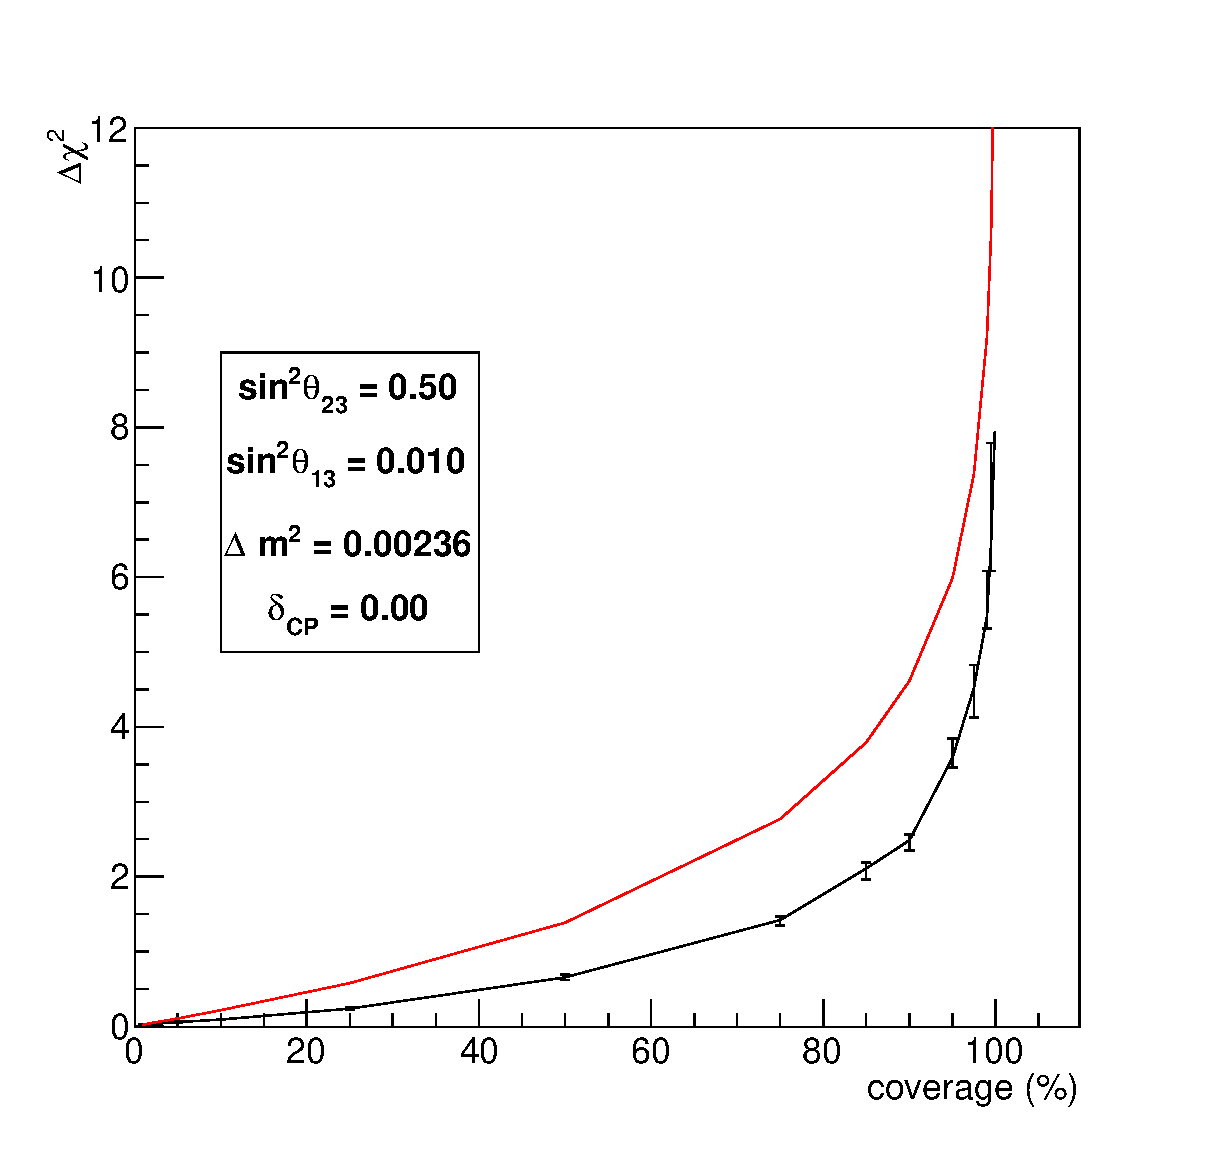
\includegraphics[width=14pc]{./images/appendix/coverage/coverage_study_2D_theta13_deltacp_syst_osc_2.eps}
%\center
%\caption {
%   Distribution of $\Delta\chi^{2}$ vs coverage in the ($sin^{2}\theta_{13}$,$\delta_{CP}$) parameter space
%  from 1k toy MC experiments generated with the Run 1+2+3 POT
% with statistical fluctuations and systematic variations at the oscillation point: 
%  $|\Delta m^{2}| = 2.36 \times 10^{-3}$,
%  $sin^{2}\theta_{23} = 0.5$,
%  $sin^{2}\theta_{13} = 0.015$ and
%  	$\delta_{CP}$	= 0.
%	}
%\label{fig:cov_2D_theta13_deltacp_syst_osc_2}
%\end{minipage}
%\hspace{0.03\linewidth}
%\begin{minipage}[t]{0.46\linewidth}
%\center
%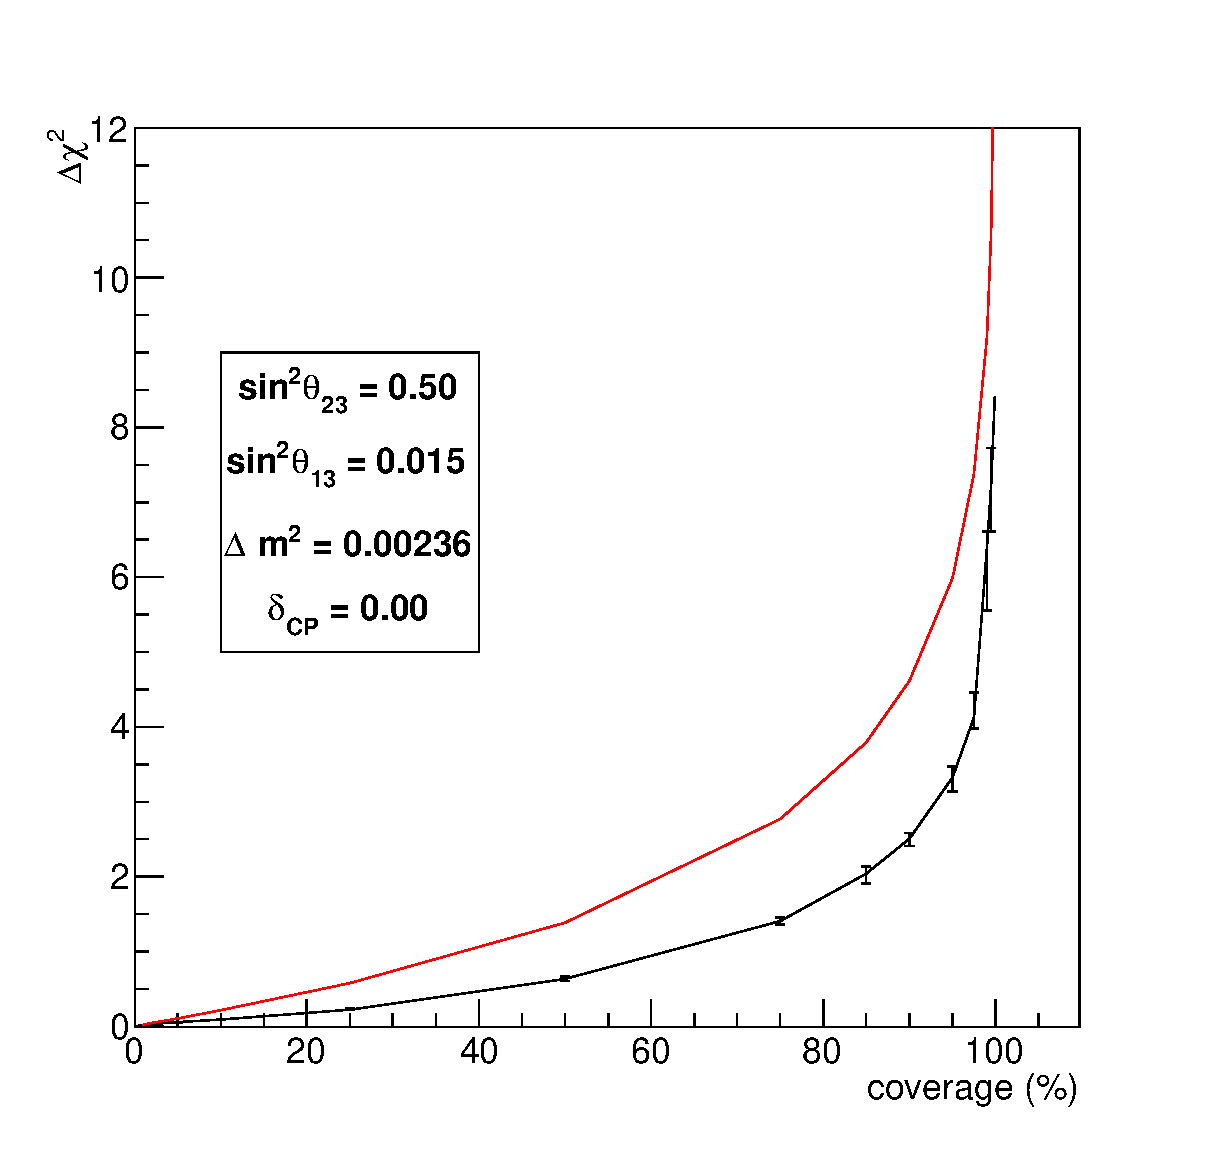
\includegraphics[width=14pc]{./images/appendix/coverage/coverage_study_2D_theta13_deltacp_syst_osc_3.eps}
%\center
%\caption {
%   Distribution of $\Delta\chi^{2}$ vs coverage in the ($sin^{2}\theta_{13}$,$\delta_{CP}$) parameter space
%  from 1k toy MC experiments generated with the Run 1+2+3 POT
%   with statistical fluctuations and systematic variations at the oscillation point: 
%  $|\Delta m^{2}| = 2.36 \times 10^{-3}$,
%  $sin^{2}\theta_{23} = 0.5$,
%  $sin^{2}\theta_{13} = 0.025$ and
%  	$\delta_{CP}$	= 0.
%	}
%\label{fig:cov_2D_theta13_deltacp_syst_osc_3}
%\end{minipage}
%\vfill
%\vspace*{0.7cm}
%\center
%\begin{minipage}[t]{0.46\linewidth}
%\center
%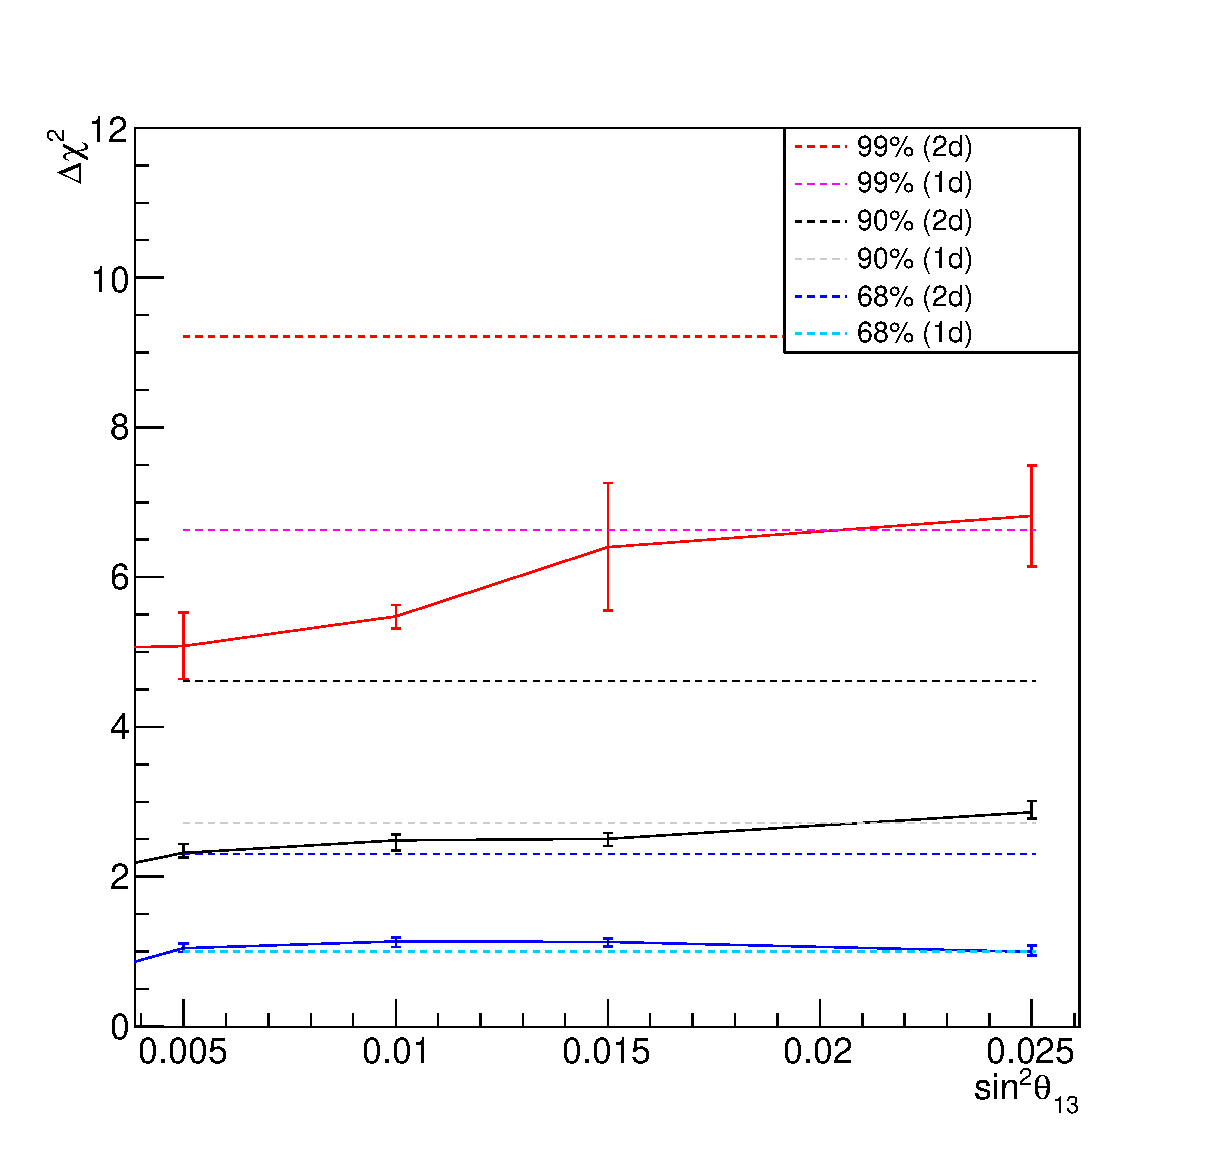
\includegraphics[width=14pc]{./images/appendix/coverage/coverage_study_2D_theta13_deltacp_syst_osc_all.eps}
%\caption {
%   Summary of figures \ref{fig:cov_2D_theta13_deltacp_syst_osc_0}-\ref{fig:cov_2D_theta13_deltacp_syst_osc_3}
%showing the value of $\Delta\chi^{2}$ at 99\%, 90\% and 68\% confidence intervals vs the value of $sin^{2}\theta_{13}$.
%	}
%\label{fig:cov_2D_theta13_deltacp_syst_osc_all}
%\end{minipage}
%\end{figure*}
%\end{center}



%% FIGURES FOR 2D theta13-theta23

%\begin{center}
%\begin{figure*}[htb]
%\begin{minipage}[t]{0.46\linewidth}
%\center
%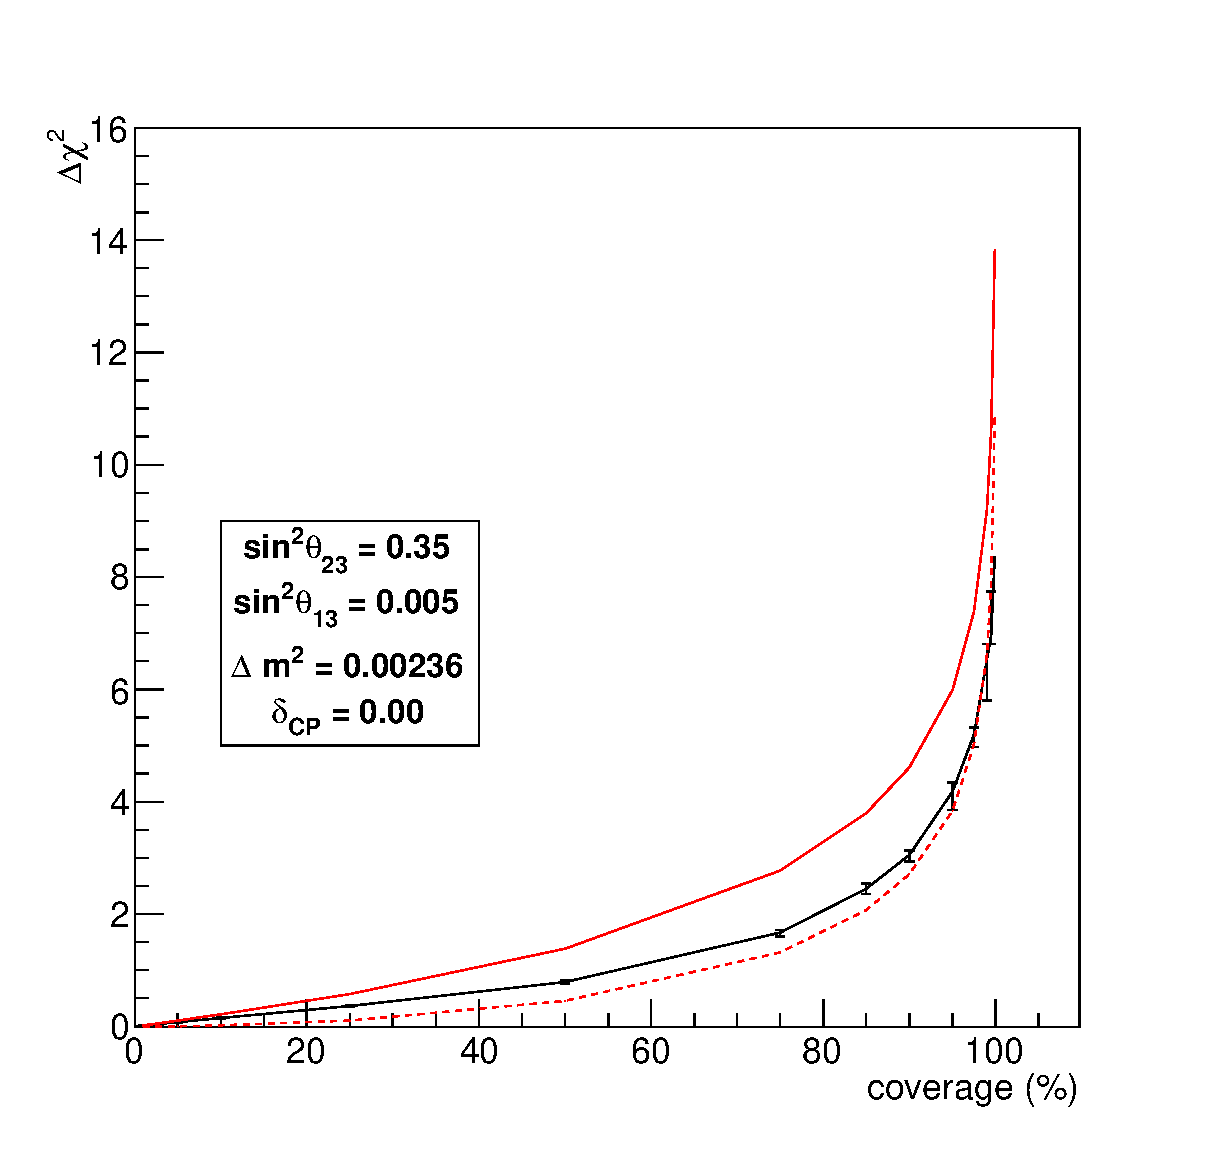
\includegraphics[width=14pc]{./images/appendix/coverage/coverage_study_2D_theta13_theta23_syst_osc_1.eps}
%\center
%\caption {
%  Distribution of $\Delta\chi^{2}$ vs coverage in the ($sin^{2}\theta_{13}$,$sin^{2}\theta_{23}$) parameter space
%  from 1k toy MC experiments generated with the Run 1+2+3 POT
% with statistical fluctuations and systematic variations at the oscillation point indicated in the legend.
%}
%\label{fig:cov_2D_theta13_theta23_syst_osc_1}
%\end{minipage}
%\hspace{0.03\linewidth}
%\begin{minipage}[t]{0.46\linewidth}
%\center
%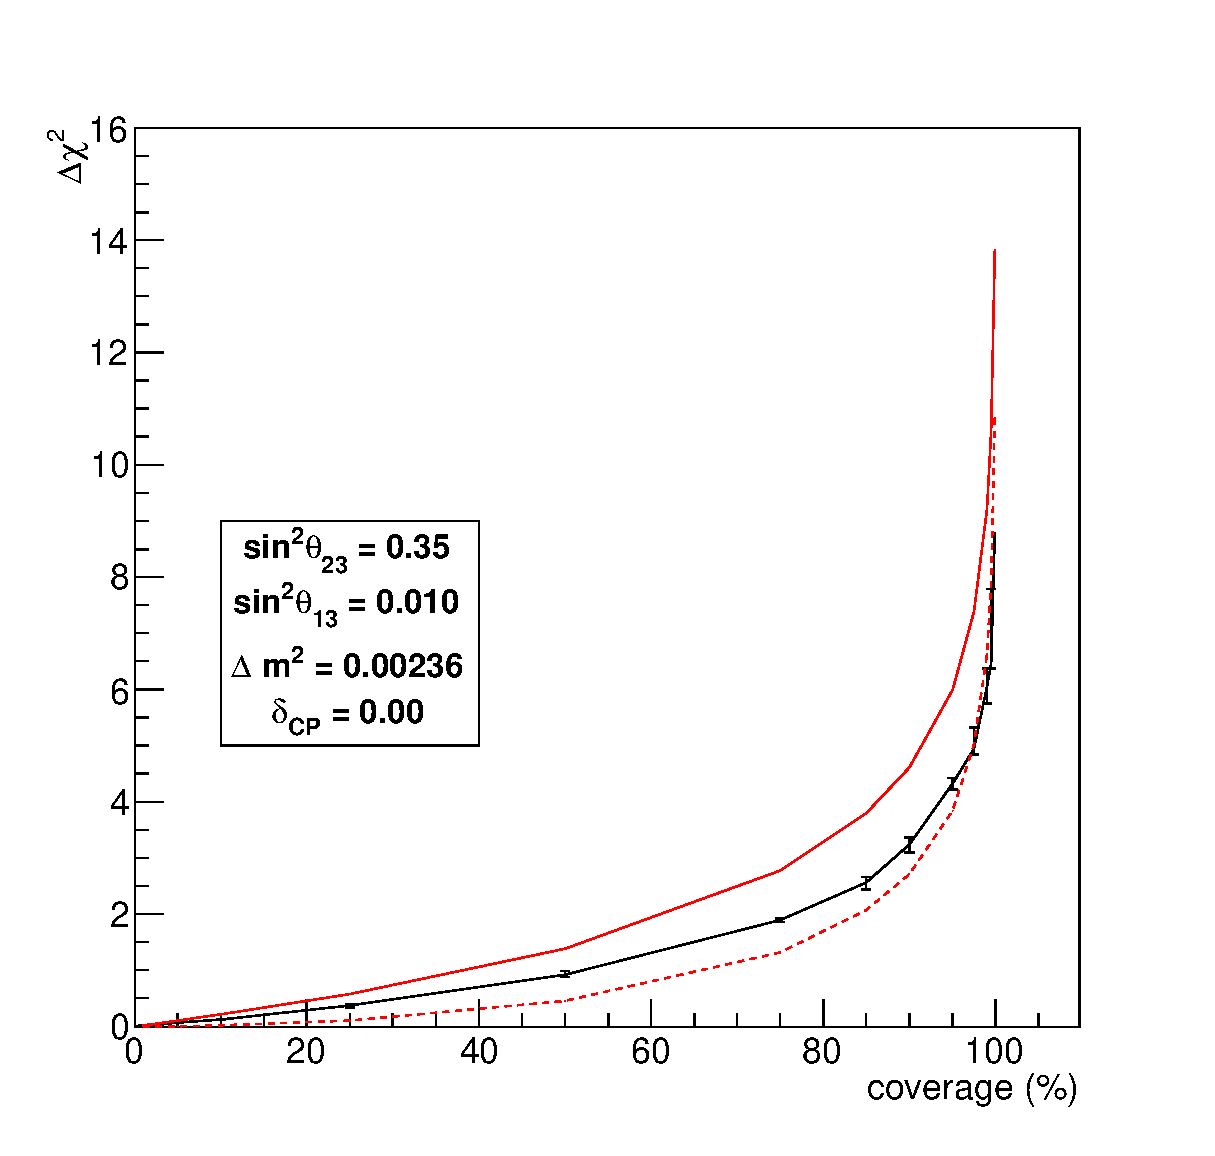
\includegraphics[width=14pc]{./images/appendix/coverage/coverage_study_2D_theta13_theta23_syst_osc_2.eps}
%\center
%\caption {
%   Distribution of $\Delta\chi^{2}$ vs coverage in the ($sin^{2}\theta_{13}$,$sin^{2}\theta_{23}$) parameter space
%  from 1k toy MC experiments generated with the Run 1+2+3 POT
% with statistical fluctuations and systematic variations at the oscillation point indicated in the legend.
%	}
%\label{fig:cov_2D_theta13_theta23_syst_osc_2}
%\end{minipage}
%\vfill
%\vspace*{0.7cm}
%\begin{minipage}[t]{0.46\linewidth}
%\center
%\includegraphics[width=14pc]{./images/appendix/coverage/coverage_study_2D_theta13_theta23_syst_osc_3.eps}
%\center
%\caption {
% Distribution of $\Delta\chi^{2}$ vs coverage in the ($sin^{2}\theta_{13}$,$sin^{2}\theta_{23}$) parameter space
%  from 1k toy MC experiments generated with the Run 1+2+3 POT
% with statistical fluctuations and systematic variations at the oscillation point indicated in the legend.
%	}
%\label{fig:cov_2D_theta13_theta23_syst_osc_3}
%\end{minipage}
%\hspace{0.03\linewidth}
%\begin{minipage}[t]{0.46\linewidth}
%\center
%\includegraphics[width=14pc]{./images/appendix/coverage/coverage_study_2D_theta13_theta23_syst_osc_4.eps}
%\center
%\caption {
%    Distribution of $\Delta\chi^{2}$ vs coverage in the ($sin^{2}\theta_{13}$,$sin^{2}\theta_{23}$) parameter space
%  from 1k toy MC experiments generated with the Run 1+2+3 POT
% with statistical fluctuations and systematic variations at the oscillation point indicated in the legend.
%	}
%\label{fig:cov_2D_theta13_theta23_syst_osc_4}
%\end{minipage}
%\vfill
%\vspace*{0.7cm}
%\begin{minipage}[t]{0.46\linewidth}
%\center
%\includegraphics[width=14pc]{./images/appendix/coverage/coverage_study_2D_theta13_theta23_syst_osc_6.eps}
%\center
%\caption {
%   Distribution of $\Delta\chi^{2}$ vs coverage in the ($sin^{2}\theta_{13}$,$sin^{2}\theta_{23}$) parameter space
%  from 1k toy MC experiments generated with the Run 1+2+3 POT
% with statistical fluctuations and systematic variations at the oscillation point indicated in the legend.
%	}
%\label{fig:cov_2D_theta13_theta23_syst_osc_6}
%\end{minipage}
%\hspace{0.03\linewidth}
%\begin{minipage}[t]{0.46\linewidth}
%\center
%\includegraphics[width=14pc]{./images/appendix/coverage/coverage_study_2D_theta13_theta23_syst_osc_7.eps}
%\center
%\caption {
%    Distribution of $\Delta\chi^{2}$ vs coverage in the ($sin^{2}\theta_{13}$,$sin^{2}\theta_{23}$) parameter space
%  from 1k toy MC experiments generated with the Run 1+2+3 POT
% with statistical fluctuations and systematic variations at the oscillation point indicated in the legend.
%		}
%\label{fig:cov_2D_theta13_theta23_syst_osc_7}
%\end{minipage}
%\end{figure*}
%\end{center}



%\begin{center}
%\begin{figure*}[htb]
%\begin{minipage}[t]{0.46\linewidth}
%\center
%\includegraphics[width=14pc]{./images/appendix/coverage/coverage_study_2D_theta13_theta23_syst_osc_8.eps}
%\center
%\caption {
%  Distribution of $\Delta\chi^{2}$ vs coverage in the ($sin^{2}\theta_{13}$,$sin^{2}\theta_{23}$) parameter space
%  from 1k toy MC experiments generated with the Run 1+2+3 POT
% with statistical fluctuations and systematic variations at the oscillation point indicated in the legend.
%}
%\label{fig:cov_2D_theta13_theta23_syst_osc_8}
%\end{minipage}
%\hspace{0.03\linewidth}
%\begin{minipage}[t]{0.46\linewidth}
%\center
%\includegraphics[width=14pc]{./images/appendix/coverage/coverage_study_2D_theta13_theta23_syst_osc_9.eps}
%\center
%\caption {
%    Distribution of $\Delta\chi^{2}$ vs coverage in the ($sin^{2}\theta_{13}$,$sin^{2}\theta_{23}$) parameter space
%  from 1k toy MC experiments generated with the Run 1+2+3 POT
% with statistical fluctuations and systematic variations at the oscillation point indicated in the legend.
%	}
%\label{fig:cov_2D_theta13_theta23_syst_osc_9}
%\end{minipage}
%\vfill
%\vspace*{0.7cm}
%\begin{minipage}[t]{0.46\linewidth}
%\center
%\includegraphics[width=14pc]{./images/appendix/coverage/coverage_study_2D_theta13_theta23_syst_osc_11.eps}
%\center
%\caption {
%   Distribution of $\Delta\chi^{2}$ vs coverage in the ($sin^{2}\theta_{13}$,$sin^{2}\theta_{23}$) parameter space
%  from 1k toy MC experiments generated with the Run 1+2+3 POT
% with statistical fluctuations and systematic variations at the oscillation point indicated in the legend.
%	}
%\label{fig:cov_2D_theta13_theta23_syst_osc_11}
%\end{minipage}
%\hspace{0.03\linewidth}
%\begin{minipage}[t]{0.46\linewidth}
%\center
%\includegraphics[width=14pc]{./images/appendix/coverage/coverage_study_2D_theta13_theta23_syst_osc_12.eps}
%\center
%\caption {
%    Distribution of $\Delta\chi^{2}$ vs coverage in the ($sin^{2}\theta_{13}$,$sin^{2}\theta_{23}$) parameter space
%  from 1k toy MC experiments generated with the Run 1+2+3 POT
% with statistical fluctuations and systematic variations at the oscillation point indicated in the legend.
%	}
%\label{fig:cov_2D_theta13_theta23_syst_osc_12}
%\end{minipage}
%\vfill
%\vspace*{0.7cm}
%\begin{minipage}[t]{0.46\linewidth}
%\center
%\includegraphics[width=14pc]{./images/appendix/coverage/coverage_study_2D_theta13_theta23_syst_osc_13.eps}
%\center
%\caption {
%    Distribution of $\Delta\chi^{2}$ vs coverage in the ($sin^{2}\theta_{13}$,$sin^{2}\theta_{23}$) parameter space
%  from 1k toy MC experiments generated with the Run 1+2+3 POT
% with statistical fluctuations and systematic variations at the oscillation point indicated in the legend.
%	}
%\label{fig:cov_2D_theta13_theta23_syst_osc_13}
%\end{minipage}
%\hspace{0.03\linewidth}
%\begin{minipage}[t]{0.46\linewidth}
%\center
%\includegraphics[width=14pc]{./images/appendix/coverage/coverage_study_2D_theta13_theta23_syst_osc_14.eps}
%\center
%\caption {
%     Distribution of $\Delta\chi^{2}$ vs coverage in the ($sin^{2}\theta_{13}$,$sin^{2}\theta_{23}$) parameter space
%  from 1k toy MC experiments generated with the Run 1+2+3 POT
% with statistical fluctuations and systematic variations at the oscillation point indicated in the legend.
%		}
%\label{fig:cov_2D_theta13_theta23_syst_osc_14}
%\end{minipage}
%\end{figure*}
%\end{center}
%
%
%
%\begin{center}
%\begin{figure*}[htb]
%\begin{minipage}[t]{0.46\linewidth}
%\center
%\includegraphics[width=14pc]{./images/appendix/coverage/coverage_study_2D_theta13_theta23_syst_osc_16.eps}
%\center
%\caption {
%   Distribution of $\Delta\chi^{2}$ vs coverage in the ($sin^{2}\theta_{13}$,$sin^{2}\theta_{23}$) parameter space
%  from 1k toy MC experiments generated with the Run 1+2+3 POT
% with statistical fluctuations and systematic variations at the oscillation point indicated in the legend.
%}
%\label{fig:cov_2D_theta13_theta23_syst_osc_16}
%\end{minipage}
%\hspace{0.03\linewidth}
%\begin{minipage}[t]{0.46\linewidth}
%\center
%\includegraphics[width=14pc]{./images/appendix/coverage/coverage_study_2D_theta13_theta23_syst_osc_17.eps}
%\center
%\caption {
% Distribution of $\Delta\chi^{2}$ vs coverage in the ($sin^{2}\theta_{13}$,$sin^{2}\theta_{23}$) parameter space
%  from 1k toy MC experiments generated with the Run 1+2+3 POT
% with statistical fluctuations and systematic variations at the oscillation point indicated in the legend.
%	}
%\label{fig:cov_2D_theta13_theta23_syst_osc_17}
%\end{minipage}
%\vfill
%\vspace*{0.7cm}
%\begin{minipage}[t]{0.46\linewidth}
%\center
%\includegraphics[width=14pc]{./images/appendix/coverage/coverage_study_2D_theta13_theta23_syst_osc_18.eps}
%\center
%\caption {
%    Distribution of $\Delta\chi^{2}$ vs coverage in the ($sin^{2}\theta_{13}$,$sin^{2}\theta_{23}$) parameter space
%  from 1k toy MC experiments generated with the Run 1+2+3 POT
% with statistical fluctuations and systematic variations at the oscillation point indicated in the legend.
%	}
%\label{fig:cov_2D_theta13_theta23_syst_osc_18}
%\end{minipage}
%\hspace{0.03\linewidth}
%\begin{minipage}[t]{0.46\linewidth}
%\center
%\includegraphics[width=14pc]{./images/appendix/coverage/coverage_study_2D_theta13_theta23_syst_osc_19.eps}
%\center
%\caption {
%  Distribution of $\Delta\chi^{2}$ vs coverage in the ($sin^{2}\theta_{13}$,$sin^{2}\theta_{23}$) parameter space
%  from 1k toy MC experiments generated with the Run 1+2+3 POT
% with statistical fluctuations and systematic variations at the oscillation point indicated in the legend.
%	}
%\label{fig:cov_2D_theta13_theta23_syst_osc_19}
%\end{minipage}
%\vfill
%\vspace*{0.7cm}


\begin{center}
\begin{figure*}[htb]
\begin{minipage}[t]{0.46\linewidth}
\center
\includegraphics[width=14pc]{./images/appendix/coverage/coverage_study_2D_theta13_theta23_stats_osc_all_1.eps}
\center
\caption {
    Summary of the values of $\Delta\chi^{2}$ at 99\%, 90\% and 68\% confidence intervals in the 2D parameter space ($sin^{2}\theta_{13}$,$sin^{2}\theta_{23}$) vs the value of $sin^{2}\theta_{23}$ with statistical fluctuations only and fitting $|\Delta m^{2}|$ and $\delta_{CP}$.
True input values for the other oscillation parameters:
$|\Delta m^{2}| = 2.36 \times 10^{-3}$ and
        $\delta_{CP}$   = 0.
	}
\label{fig:cov_2D_theta13_theta23_stats_osc_all_1}
\end{minipage}
\hspace{0.03\linewidth}
\begin{minipage}[t]{0.46\linewidth}
\center
\includegraphics[width=14pc]{./images/appendix/coverage/coverage_study_2D_theta13_theta23_stats_osc_new_all_1.eps}
\center
\caption {
    Summary of the values of cumulative probability  for $\Delta\chi^{2}=9.21$ (canonical value for 99\%), $\Delta\chi^{2}=4.61$ (canonical value for 90\%) and $\Delta\chi^{2}=2.30$ (canonical value for 68\%) in the 2D parameter space ($sin^{2}\theta_{13}$,$sin^{2}\theta_{23}$) vs the value of $sin^{2}\theta_{23}$ with statistical fluctuations only and fitting $|\Delta m^{2}|$ and $\delta_{CP}$.
True input values for the other oscillation parameters:
$|\Delta m^{2}| = 2.36 \times 10^{-3}$ and
        $\delta_{CP}$   = 0.
	}
\label{fig:prob_2D_theta13_theta23_stats_osc_all_1}
\end{minipage}
\vfill
\vspace*{0.7cm}
\begin{minipage}[t]{0.46\linewidth}
\center
\includegraphics[width=14pc]{./images/appendix/coverage/coverage_study_2D_theta13_theta23_syst_osc_all_1.eps}
\center
\caption {
   Summary of the values of $\Delta\chi^{2}$ at 99\%, 90\% and 68\% confidence intervals in the 2D parameter space ($sin^{2}\theta_{13}$,$sin^{2}\theta_{23}$) vs the value of $sin^{2}\theta_{23}$ with statistical fluctuations and systematic variations and fitting $|\Delta m^{2}|$ and $\delta_{CP}$.
True input values for the other oscillation parameters:
$|\Delta m^{2}| = 2.36 \times 10^{-3}$ and
        $\delta_{CP}$   = 0.
		}
\label{fig:cov_2D_theta13_theta23_syst_osc_all_1}
\end{minipage}
\hspace{0.03\linewidth}
\begin{minipage}[t]{0.46\linewidth}
\center
\includegraphics[width=14pc]{./images/appendix/coverage/coverage_study_2D_theta13_theta23_syst_osc_new_all_1.eps}
\center
\caption {
    Summary of the values of cumulative probability  for $\Delta\chi^{2}=9.21$ (canonical value for 99\%), $\Delta\chi^{2}=4.61$ (canonical value for 90\%) and $\Delta\chi^{2}=2.30$ (canonical value for 68\%) in the 2D parameter space ($sin^{2}\theta_{13}$,$sin^{2}\theta_{23}$) vs the value of $sin^{2}\theta_{23}$ with statistical fluctuations and systematic variations and fitting $|\Delta m^{2}|$ and $\delta_{CP}$.
True input values for the other oscillation parameters:
$|\Delta m^{2}| = 2.36 \times 10^{-3}$ and
        $\delta_{CP}$   = 0.
	}
\label{fig:prob_2D_theta13_theta23_syst_osc_all_1}
\end{minipage}
\end{figure*}
\end{center}


\begin{center}
\begin{figure*}[htb]
\begin{minipage}[t]{0.46\linewidth}
\center
\includegraphics[width=14pc]{./images/appendix/coverage/coverage_study_2D_theta13_theta23_stats_osc_all_2.eps}
\center
\caption {
    Summary of the values of $\Delta\chi^{2}$ at 99\%, 90\% and 68\% confidence intervals in the 2D parameter space ($sin^{2}\theta_{13}$,$sin^{2}\theta_{23}$) vs the value of $sin^{2}\theta_{13}$ with statistical fluctuations only and fitting $|\Delta m^{2}|$ and $\delta_{CP}$.
True input values for the other oscillation parameters:
$|\Delta m^{2}| = 2.36 \times 10^{-3}$ and
        $\delta_{CP}$   = 0.
	}
\label{fig:cov_2D_theta13_theta23_stats_osc_all_2}
\end{minipage}
\hspace{0.03\linewidth}
\begin{minipage}[t]{0.46\linewidth}
\center
\includegraphics[width=14pc]{./images/appendix/coverage/coverage_study_2D_theta13_theta23_stats_osc_new_all_2.eps}
\center
\caption {
    Summary of the values of cumulative probability  for $\Delta\chi^{2}=9.21$ (canonical value for 99\%), $\Delta\chi^{2}=4.61$ (canonical value for 90\%) and $\Delta\chi^{2}=2.30$ (canonical value for 68\%) in the 2D parameter space ($sin^{2}\theta_{13}$,$sin^{2}\theta_{23}$) vs the value of $sin^{2}\theta_{13}$ with statistical fluctuations only and fitting $|\Delta m^{2}|$ and $\delta_{CP}$.
True input values for the other oscillation parameters:
$|\Delta m^{2}| = 2.36 \times 10^{-3}$ and
        $\delta_{CP}$   = 0.
	}
\label{fig:prob_2D_theta13_theta23_stats_osc_all_2}
\end{minipage}
\vfill
\vspace*{0.7cm}
\begin{minipage}[t]{0.46\linewidth}
\center
\includegraphics[width=14pc]{./images/appendix/coverage/coverage_study_2D_theta13_theta23_syst_osc_all_2.eps}
\center
\caption {
   Summary of the values of $\Delta\chi^{2}$ at 99\%, 90\% and 68\% confidence intervals in the 2D parameter space ($sin^{2}\theta_{13}$,$sin^{2}\theta_{23}$) vs the value of $sin^{2}\theta_{13}$ with statistical fluctuations and systematic variations and fitting $|\Delta m^{2}|$ and $\delta_{CP}$.
True input values for the other oscillation parameters:
$|\Delta m^{2}| = 2.36 \times 10^{-3}$ and
        $\delta_{CP}$   = 0.
		}
\label{fig:cov_2D_theta13_theta23_syst_osc_all_2}
\end{minipage}
\hspace{0.03\linewidth}
\begin{minipage}[t]{0.46\linewidth}
\center
\includegraphics[width=14pc]{./images/appendix/coverage/coverage_study_2D_theta13_theta23_syst_osc_new_all_2.eps}
\center
\caption {
    Summary of the values of cumulative probability  for $\Delta\chi^{2}=9.21$ (canonical value for 99\%), $\Delta\chi^{2}=4.61$ (canonical value for 90\%) and $\Delta\chi^{2}=2.30$ (canonical value for 68\%) in the 2D parameter space ($sin^{2}\theta_{13}$,$sin^{2}\theta_{23}$) vs the value of $sin^{2}\theta_{13}$ with statistical fluctuations and systematic variations and fitting $|\Delta m^{2}|$ and $\delta_{CP}$.
True input values for the other oscillation parameters:
$|\Delta m^{2}| = 2.36 \times 10^{-3}$ and
        $\delta_{CP}$   = 0.
	}
\label{fig:prob_2D_theta13_theta23_syst_osc_all_2}
\end{minipage}
\end{figure*}
\end{center}


%%%LORENA -
\begin{center}
\begin{figure*}[htb]
\begin{minipage}[t]{0.46\linewidth}
\center
\includegraphics[width=14pc]{./images/appendix/coverage/coverage_study_2D_theta13_theta23_stats_osc_68.eps}
\center
\caption {
    Summary of values of $\Delta\chi^{2}$ at 68\% confidence intervals in Z axis (color) in the 2D parameter space ($sin^{2}\theta_{13}$,$sin^{2}\theta_{23}$) vs the value of $sin^{2}\theta_{23}$ in X axis and $sin^{2}\theta_{13}$ in Y axis for toy experiments with statistical fluctuations only and fitting $|\Delta m^{2}|$ and $\delta_{CP}$.
True input values for the other oscillation parameters:
$|\Delta m^{2}| = 2.36 \times 10^{-3}$ and
        $\delta_{CP}$   = 0.
	}
\label{fig:cov_2D_theta13_theta23_stats_osc_68}
\end{minipage}
\hspace{0.03\linewidth}
\begin{minipage}[t]{0.46\linewidth}
\center
\includegraphics[width=14pc]{./images/appendix/coverage/coverage_study_2D_theta13_theta23_stats_osc_new_68.eps}
\center
\caption {
    Summary of values of cumulative probability at $\Delta\chi^{2} = 2.30$ in Z axis (color) in the 2D parameter space ($sin^{2}\theta_{13}$,$sin^{2}\theta_{23}$) vs the value of $sin^{2}\theta_{23}$ in X axis and $sin^{2}\theta_{13}$ in Y axis for toy experiments with statistical fluctuations only and fitting $|\Delta m^{2}|$ and $\delta_{CP}$.
True input values for the other oscillation parameters:
$|\Delta m^{2}| = 2.36 \times 10^{-3}$ and
        $\delta_{CP}$   = 0.
	}
\label{fig:prob_2D_theta13_theta23_stats_osc_68}
\end{minipage}
\vfill
\vspace*{0.7cm}
\begin{minipage}[t]{0.46\linewidth}
\center
\includegraphics[width=14pc]{./images/appendix/coverage/coverage_study_2D_theta13_theta23_stats_osc_90.eps}
\center
\caption {
    Summary of values of $\Delta\chi^{2}$ at 90\% confidence intervals in Z axis (color) in the 2D parameter space ($sin^{2}\theta_{13}$,$sin^{2}\theta_{23}$) vs the value of $sin^{2}\theta_{23}$ in X axis and $sin^{2}\theta_{13}$ in Y axis for toy experiments with statistical fluctuations only and fitting $|\Delta m^{2}|$ and $\delta_{CP}$.
True input values for the other oscillation parameters:
$|\Delta m^{2}| = 2.36 \times 10^{-3}$ and
        $\delta_{CP}$   = 0.
	}
\label{fig:cov_2D_theta13_theta23_stats_osc_90}
\end{minipage}
\hspace{0.03\linewidth}
\begin{minipage}[t]{0.46\linewidth}
\center
\includegraphics[width=14pc]{./images/appendix/coverage/coverage_study_2D_theta13_theta23_stats_osc_new_90.eps}
\center
\caption {
    Summary of values of cumulative probability at $\Delta\chi^{2} = 4.61$ in Z axis (color) in the 2D parameter space ($sin^{2}\theta_{13}$,$sin^{2}\theta_{23}$) vs the value of $sin^{2}\theta_{23}$ in X axis and $sin^{2}\theta_{13}$ in Y axis for toy experiments with statistical fluctuations only and fitting $|\Delta m^{2}|$ and $\delta_{CP}$.
True input values for the other oscillation parameters:
$|\Delta m^{2}| = 2.36 \times 10^{-3}$ and
        $\delta_{CP}$   = 0.
	}
\label{fig:prob_2D_theta13_theta23_stats_osc_90}
\end{minipage}
\vfill
\vspace*{0.7cm}
\begin{minipage}[t]{0.46\linewidth}
\center
\includegraphics[width=14pc]{./images/appendix/coverage/coverage_study_2D_theta13_theta23_stats_osc_99.eps}
\center
\caption {
    Summary of values of $\Delta\chi^{2}$ at 99\% confidence intervals in Z axis (color) in the 2D parameter space ($sin^{2}\theta_{13}$,$sin^{2}\theta_{23}$) vs the value of $sin^{2}\theta_{23}$ in X axis and $sin^{2}\theta_{13}$ in Y axis for toy experiments with statistical fluctuations only and fitting $|\Delta m^{2}|$ and $\delta_{CP}$.
True input values for the other oscillation parameters:
$|\Delta m^{2}| = 2.36 \times 10^{-3}$ and
        $\delta_{CP}$   = 0.
	}
\label{fig:cov_2D_theta13_theta23_stats_osc_99}
\end{minipage}
\hspace{0.03\linewidth}
\begin{minipage}[t]{0.46\linewidth}
\center
\includegraphics[width=14pc]{./images/appendix/coverage/coverage_study_2D_theta13_theta23_stats_osc_new_99.eps}
\center
\caption {
    Summary of values of cumulative probability at $\Delta\chi^{2} = 9.21$ in Z axis (color) in the 2D parameter space ($sin^{2}\theta_{13}$,$sin^{2}\theta_{23}$) vs the value of $sin^{2}\theta_{23}$ in X axis and $sin^{2}\theta_{13}$ in Y axis for toy experiments with statistical fluctuations only and fitting $|\Delta m^{2}|$ and $\delta_{CP}$.
True input values for the other oscillation parameters:
$|\Delta m^{2}| = 2.36 \times 10^{-3}$ and
        $\delta_{CP}$   = 0.
	}
\label{fig:prob_2D_theta13_theta23_stats_osc_99}
\end{minipage}
\end{figure*}
\end{center}


\begin{center}
\begin{figure*}[htb]
\begin{minipage}[t]{0.46\linewidth}
\center
\includegraphics[width=14pc]{./images/appendix/coverage/coverage_study_2D_theta13_theta23_syst_osc_68.eps}
\center
\caption {
    Summary of values of $\Delta\chi^{2}$ at 68\% confidence intervals in Z axis (color) in the 2D parameter space ($sin^{2}\theta_{13}$,$sin^{2}\theta_{23}$) vs the value of $sin^{2}\theta_{23}$ in X axis and $sin^{2}\theta_{13}$ in Y axis for toy experiments with statistical fluctuations and systematic variations and fitting $|\Delta m^{2}|$ and $\delta_{CP}$.
True input values for the other oscillation parameters:
$|\Delta m^{2}| = 2.36 \times 10^{-3}$ and
        $\delta_{CP}$   = 0.
	}
\label{fig:cov_2D_theta13_theta23_syst_osc_68}
\end{minipage}
\hspace{0.03\linewidth}
\begin{minipage}[t]{0.46\linewidth}
\center
\includegraphics[width=14pc]{./images/appendix/coverage/coverage_study_2D_theta13_theta23_syst_osc_new_68.eps}
\center
\caption {
    Summary of values of cumulative probability at $\Delta\chi^{2} = 2.30$ in Z axis (color) in the 2D parameter space ($sin^{2}\theta_{13}$,$sin^{2}\theta_{23}$) vs the value of $sin^{2}\theta_{23}$ in X axis and $sin^{2}\theta_{13}$ in Y axis for toy experiments with statistical fluctuations and systematic variations and fitting $|\Delta m^{2}|$ and $\delta_{CP}$.
True input values for the other oscillation parameters:
$|\Delta m^{2}| = 2.36 \times 10^{-3}$ and
        $\delta_{CP}$   = 0.
	}
\label{fig:prob_2D_theta13_theta23_syst_osc_68}
\end{minipage}
\vfill
\vspace*{0.7cm}
\begin{minipage}[t]{0.46\linewidth}
\center
\includegraphics[width=14pc]{./images/appendix/coverage/coverage_study_2D_theta13_theta23_syst_osc_90.eps}
\center
\caption {
    Summary of values of $\Delta\chi^{2}$ at 90\% confidence intervals in Z axis (color) in the 2D parameter space ($sin^{2}\theta_{13}$,$sin^{2}\theta_{23}$) vs the value of $sin^{2}\theta_{23}$ in X axis and $sin^{2}\theta_{13}$ in Y axis for toy experiments with statistical fluctuations and systematic variations and fitting $|\Delta m^{2}|$ and $\delta_{CP}$.
True input values for the other oscillation parameters:
$|\Delta m^{2}| = 2.36 \times 10^{-3}$ and
        $\delta_{CP}$   = 0.
	}
\label{fig:cov_2D_theta13_theta23_syst_osc_90}
\end{minipage}
\hspace{0.03\linewidth}
\begin{minipage}[t]{0.46\linewidth}
\center
\includegraphics[width=14pc]{./images/appendix/coverage/coverage_study_2D_theta13_theta23_syst_osc_new_90.eps}
\center
\caption {
    Summary of values of cumulative probability at $\Delta\chi^{2} = 4.61$ in Z axis (color) in the 2D parameter space ($sin^{2}\theta_{13}$,$sin^{2}\theta_{23}$) vs the value of $sin^{2}\theta_{23}$ in X axis and $sin^{2}\theta_{13}$ in Y axis for toy experiments with statistical fluctuations and systematic variations and fitting $|\Delta m^{2}|$ and $\delta_{CP}$.
True input values for the other oscillation parameters:
$|\Delta m^{2}| = 2.36 \times 10^{-3}$ and
        $\delta_{CP}$   = 0.
	}
\label{fig:prob_2D_theta13_theta23_syst_osc_90}
\end{minipage}
\vfill
\vspace*{0.7cm}
\begin{minipage}[t]{0.46\linewidth}
\center
\includegraphics[width=14pc]{./images/appendix/coverage/coverage_study_2D_theta13_theta23_syst_osc_99.eps}
\center
\caption {
    Summary of values of $\Delta\chi^{2}$ at 99\% confidence intervals in Z axis (color) in the 2D parameter space ($sin^{2}\theta_{13}$,$sin^{2}\theta_{23}$) vs the value of $sin^{2}\theta_{23}$ in X axis and $sin^{2}\theta_{13}$ in Y axis for toy experiments with statistical fluctuations and systematic variations and fitting $|\Delta m^{2}|$ and $\delta_{CP}$.
True input values for the other oscillation parameters:
$|\Delta m^{2}| = 2.36 \times 10^{-3}$ and
        $\delta_{CP}$   = 0.
	}
\label{fig:cov_2D_theta13_theta23_syst_osc_99}
\end{minipage}
\hspace{0.03\linewidth}
\begin{minipage}[t]{0.46\linewidth}
\center
\includegraphics[width=14pc]{./images/appendix/coverage/coverage_study_2D_theta13_theta23_syst_osc_new_99.eps}
\center
\caption {
    Summary of values of cumulative probability at $\Delta\chi^{2} = 9.21$ in Z axis (color) in the 2D parameter space ($sin^{2}\theta_{13}$,$sin^{2}\theta_{23}$) vs the value of $sin^{2}\theta_{23}$ in X axis and $sin^{2}\theta_{13}$ in Y axis for toy experiments with statistical fluctuations and systematic variations and fitting $|\Delta m^{2}|$ and $\delta_{CP}$.
True input values for the other oscillation parameters:
$|\Delta m^{2}| = 2.36 \times 10^{-3}$ and
        $\delta_{CP}$   = 0.
	}
\label{fig:prob_2D_theta13_theta23_syst_osc_99}
\end{minipage}
\end{figure*}
\end{center}


\begin{center}
\begin{figure*}[htb]
\center
\begin{minipage}[t]{0.46\linewidth}
\center
\includegraphics[width=14pc]{./images/appendix/coverage/coverage_study_2D_theta13_dm23sq_stats_fixed_all_extra.eps}
\caption {
   Summary of the values of $\Delta\chi^{2}$ at 99\%, 90\% and 68\% confidence intervals in the 2D parameter space ($sin^{2}\theta_{13}$,$|\Delta m^{2}|$) vs the value of $sin^{2}\theta_{13}$ with statistical fluctuations only and {\bf{fixing $sin^{2}\theta_{23}$ and $\delta_{CP}$}}.
True input values for the other oscillation parameters:
$|\Delta m^{2}| = 2.36 \times 10^{-3}$,
  $sin^{2}\theta_{23} = 0.35$ and
        $\delta_{CP}$   = 0.
	}
\label{fig:cov_2D_theta13_dmsq_stats_fixed_all_extra}
\end{minipage}
\vfill
 \vspace*{0.7cm}
\begin{minipage}[t]{0.46\linewidth}
\center
\includegraphics[width=14pc]{./images/appendix/coverage/coverage_study_2D_theta13_dm23sq_stats_theta23_all_extra.eps}
\caption {
   Summary of the values of $\Delta\chi^{2}$ at 99\%, 90\% and 68\% confidence intervals  in the 2D parameter space ($sin^{2}\theta_{13}$,$|\Delta m^{2}|$) vs the value of $sin^{2}\theta_{13}$ with statistical fluctuations only and {\bf{fitting $sin^{2}\theta_{23}$ and fixing $\delta_{CP}$}}.
True input values for the other oscillation parameters:
$|\Delta m^{2}| = 2.36 \times 10^{-3}$,
  $sin^{2}\theta_{23} = 0.35$ and
        $\delta_{CP}$   = 0.
	}
\label{fig:cov_2D_theta13_dmsq_stats_theta23_all_extra}
\end{minipage}
\hspace{0.03\linewidth}
\begin{minipage}[t]{0.46\linewidth}
\center
\includegraphics[width=14pc]{./images/appendix/coverage/coverage_study_2D_theta13_dm23sq_stats_deltacp_all_extra.eps}
\caption {
   Summary of the values of $\Delta\chi^{2}$ at 99\%, 90\% and 68\% confidence intervals  in the 2D parameter space ($sin^{2}\theta_{13}$,$|\Delta m^{2}|$) vs the value of $sin^{2}\theta_{13}$ with statistical fluctuations only and {\bf{fitting $\delta_{CP}$ and fixing $sin^{2}\theta_{23}$}}.
True input values for the other oscillation parameters:
$|\Delta m^{2}| = 2.36 \times 10^{-3}$,
  $sin^{2}\theta_{23} = 0.35$ and
        $\delta_{CP}$   = 0.
	}
\label{fig:cov_2D_theta13_dmsq_stats_deltacp_all_extra}
\end{minipage}
\vfill
 \vspace*{0.7cm}
\begin{minipage}[t]{0.46\linewidth}
\center
\includegraphics[width=14pc]{./images/appendix/coverage/coverage_study_2D_theta13_dm23sq_stats_osc_all_extra.eps}
\caption {
   Summary of the values of $\Delta\chi^{2}$ at 99\%, 90\% and 68\% confidence intervals  in the 2D parameter space ($sin^{2}\theta_{13}$,$|\Delta m^{2}|$) vs the value of $sin^{2}\theta_{13}$ with statistical fluctuations only and {\bf{fitting $sin^{2}\theta_{23}$ and $\delta_{CP}$}}.
True input values for the other oscillation parameters:
$|\Delta m^{2}| = 2.36 \times 10^{-3}$,
  $sin^{2}\theta_{23} = 0.35$ and
        $\delta_{CP}$   = 0.
	}
\label{fig:cov_2D_theta13_dmsq_stats_osc_all_extra}
\end{minipage}
\hspace{0.03\linewidth}
\begin{minipage}[t]{0.46\linewidth}
\center
\includegraphics[width=14pc]{./images/appendix/coverage/coverage_study_2D_theta13_dm23sq_syst_osc_all_extra.eps}
\caption {
   Summary of the values of $\Delta\chi^{2}$ at 99\%, 90\% and 68\% confidence intervals  in the 2D parameter space ($sin^{2}\theta_{13}$,$|\Delta m^{2}|$) vs the value of $sin^{2}\theta_{13}$ with statistical fluctuations and systematic variations and {\bf{fitting $sin^{2}\theta_{23}$ and $\delta_{CP}$}}.
True input values for the other oscillation parameters:
$|\Delta m^{2}| = 2.36 \times 10^{-3}$,
  $sin^{2}\theta_{23} = 0.35$ and
        $\delta_{CP}$   = 0.
	}
\label{fig:cov_2D_theta13_dmsq_syst_osc_all_extra}

\end{minipage}
\end{figure*}
\end{center}


\begin{center}
\begin{figure*}[htb]
\center
\begin{minipage}[t]{0.46\linewidth}
\center
\includegraphics[width=14pc]{./images/appendix/coverage/coverage_study_2D_theta13_dm23sq_stats_fixed_all_extra_new.eps}
\caption {
   Summary of cumulative probability  for $\Delta\chi^{2}=9.21$ (canonical value for 99\%), $\Delta\chi^{2}=4.61$ (canonical value for 90\%) and $\Delta\chi^{2}=2.30$ (canonical value for 68\%) in the 2D parameter space ($sin^{2}\theta_{13}$,$|\Delta m^{2}|$) vs the value of $sin^{2}\theta_{13}$ with statistical fluctuations only and {\bf{fixing $sin^{2}\theta_{23}$ and $\delta_{CP}$}}.
True input values for the other oscillation parameters:
$|\Delta m^{2}| = 2.36 \times 10^{-3}$,
  $sin^{2}\theta_{23} = 0.35$ and
        $\delta_{CP}$   = 0.
	}
\label{fig:prob_2D_theta13_dmsq_stats_fixed_all_extra}
\end{minipage}
\vfill
 \vspace*{0.7cm}
\begin{minipage}[t]{0.46\linewidth}
\center
\includegraphics[width=14pc]{./images/appendix/coverage/coverage_study_2D_theta13_dm23sq_stats_theta23_all_extra_new.eps}
\caption {
   Summary of cumulative probability  for $\Delta\chi^{2}=9.21$ (canonical value for 99\%), $\Delta\chi^{2}=4.61$ (canonical value for 90\%) and $\Delta\chi^{2}=2.30$ (canonical value for 68\%) in the 2D parameter space ($sin^{2}\theta_{13}$,$|\Delta m^{2}|$) vs the value of $sin^{2}\theta_{13}$ with statistical fluctuations only and {\bf{fitting $sin^{2}\theta_{23}$ and fixing $\delta_{CP}$}}.
True input values for the other oscillation parameters:
$|\Delta m^{2}| = 2.36 \times 10^{-3}$,
  $sin^{2}\theta_{23} = 0.35$ and
        $\delta_{CP}$   = 0.
	}
\label{fig:prob_2D_theta13_dmsq_stats_theta23_all_extra}
\end{minipage}
\hspace{0.03\linewidth}
\begin{minipage}[t]{0.46\linewidth}
\center
\includegraphics[width=14pc]{./images/appendix/coverage/coverage_study_2D_theta13_dm23sq_stats_deltacp_all_extra_new.eps}
\caption {
   Summary of cumulative probability  for $\Delta\chi^{2}=9.21$ (canonical value for 99\%), $\Delta\chi^{2}=4.61$ (canonical value for 90\%) and $\Delta\chi^{2}=2.30$ (canonical value for 68\%) in the 2D parameter space ($sin^{2}\theta_{13}$,$|\Delta m^{2}|$) vs the value of $sin^{2}\theta_{13}$ with statistical fluctuations only and {\bf{fitting $\delta_{CP}$ and fixing $sin^{2}\theta_{23}$}}.
True input values for the other oscillation parameters:
$|\Delta m^{2}| = 2.36 \times 10^{-3}$,
  $sin^{2}\theta_{23} = 0.35$ and
        $\delta_{CP}$   = 0.
	}
\label{fig:prob_2D_theta13_dmsq_stats_deltacp_all_extra}
\end{minipage}
\vfill
 \vspace*{0.7cm}
\begin{minipage}[t]{0.46\linewidth}
\center
\includegraphics[width=14pc]{./images/appendix/coverage/coverage_study_2D_theta13_dm23sq_stats_osc_all_extra_new.eps}
\caption {
   Summary of cumulative probability  for $\Delta\chi^{2}=9.21$ (canonical value for 99\%), $\Delta\chi^{2}=4.61$ (canonical value for 90\%) and $\Delta\chi^{2}=2.30$ (canonical value for 68\%) in the 2D parameter space ($sin^{2}\theta_{13}$,$|\Delta m^{2}|$) vs the value of $sin^{2}\theta_{13}$ with statistical fluctuations only and {\bf{fitting $sin^{2}\theta_{23}$ and $\delta_{CP}$}}.
True input values for the other oscillation parameters:
$|\Delta m^{2}| = 2.36 \times 10^{-3}$,
  $sin^{2}\theta_{23} = 0.35$ and
        $\delta_{CP}$   = 0.
	}
\label{fig:prob_2D_theta13_dmsq_stats_osc_all_extra}
\end{minipage}
\hspace{0.03\linewidth}
\begin{minipage}[t]{0.46\linewidth}
\center
\includegraphics[width=14pc]{./images/appendix/coverage/coverage_study_2D_theta13_dm23sq_syst_osc_all_extra_new.eps}
\caption {
   Summary of cumulative probability  for $\Delta\chi^{2}=9.21$ (canonical value for 99\%), $\Delta\chi^{2}=4.61$ (canonical value for 90\%) and $\Delta\chi^{2}=2.30$ (canonical value for 68\%) in the 2D parameter space ($sin^{2}\theta_{13}$,$|\Delta m^{2}|$) vs the value of $sin^{2}\theta_{13}$ with statistical fluctuations and systematic variations and {\bf{fitting $sin^{2}\theta_{23}$ and $\delta_{CP}$}}.
True input values for the other oscillation parameters:
$|\Delta m^{2}| = 2.36 \times 10^{-3}$,
  $sin^{2}\theta_{23} = 0.35$ and
        $\delta_{CP}$   = 0.
	}
\label{fig:prob_2D_theta13_dmsq_syst_osc_all_extra}
\end{minipage}
\end{figure*}
\end{center}


\begin{center}
\begin{figure*}[htb]
\center
\begin{minipage}[t]{0.46\linewidth}
\center
\includegraphics[width=14pc]{./images/appendix/coverage/coverage_study_1D_stats_deltacp_theta23_all.eps}
\caption {
   Summary of the values of $\Delta\chi^{2}$ at 99\%, 90\% and 68\% confidence intervals in the 1D parameter space $sin^{2}\theta_{23}$ vs the value of $sin^{2}\theta_{23}$ with statistical fluctuations only where $\Delta\chi^{2}$ was calculated as folllows: a first fit was done fitting only $\delta_{CP}$, fixing the other three oscillation parameters to their true input value, and $\chi^{2}_{init}$ was obtained; then a second fit was done fitting $\delta_{CP}$ and $sin^{2}\theta_{23}$, keeping $sin^{2}\theta_{13}$ and $|\Delta m^{2}|$ fixed to their true input values and $\chi^{2}_{bf}$ was obtained, computing finally $\Delta\chi^{2} = \chi^{2}_{init} - \chi^{2}_{bf}$.
True input values for the other oscillation parameters:
$|\Delta m^{2}| = 2.36 \times 10^{-3}$,
  $sin^{2}\theta_{13} = 0.025$ and
        $\delta_{CP}$   = 0.
	}
\label{fig:cov_1D_deltacp_theta23_all}
\end{minipage}
\hspace{0.03\linewidth}
\begin{minipage}[t]{0.46\linewidth}
\center
\includegraphics[width=14pc]{./images/appendix/coverage/coverage_study_1D_stats_deltacp_dm23sq_all.eps}
\caption {
   Summary of the values of $\Delta\chi^{2}$ at 99\%, 90\% and 68\% confidence intervals in the 1D parameter space $|\Delta m^{2}|$ vs the value of $|\Delta m^{2}|$ with statistical fluctuations only where $\Delta\chi^{2}$ was calculated as folllows: a first fit was done fitting only $\delta_{CP}$, fixing the other three oscillation parameters to their true input value, and $\chi^{2}_{init}$ was obtained; then a second fit was done fitting $\delta_{CP}$ and $|\Delta m^{2}|$, keeping $sin^{2}\theta_{13}$ and $sin^{2}\theta_{23}$ fixed to their true input values and $\chi^{2}_{bf}$ was obtained, computing finally $\Delta\chi^{2} = \chi^{2}_{init} - \chi^{2}_{bf}$.
True input values for the other oscillation parameters:
  $sin^{2}\theta_{23} = 0.5$, 
$sin^{2}\theta_{13} = 0.025$ and
        $\delta_{CP}$   = 0.
	}
\label{fig:cov_1D_deltacp_dmsq_all}
\end{minipage}
\vfill
 \vspace*{0.7cm}
\begin{minipage}[t]{0.46\linewidth}
\center
\includegraphics[width=14pc]{./images/appendix/coverage/coverage_study_1D_stats_deltacp_theta13_all.eps}
\caption {
    Summary of the values of $\Delta\chi^{2}$ at 99\%, 90\% and 68\% confidence intervals in the 1D parameter space $sin^{2}\theta_{13}$ vs the value of $sin^{2}\theta_{13}$ with statistical fluctuations only where $\Delta\chi^{2}$ was calculated as folllows: a first fit was done fitting only $\delta_{CP}$, fixing the other three oscillation parameters to their true input value, and $\chi^{2}_{init}$ was obtained; then a second fit was done fitting $\delta_{CP}$ and $sin^{2}\theta_{13}$, keeping $sin^{2}\theta_{23}$ and $|\Delta m^{2}|$ fixed to their true input values and $\chi^{2}_{bf}$ was obtained, computing finally $\Delta\chi^{2} = \chi^{2}_{init} - \chi^{2}_{bf}$.
True input values for the other oscillation parameters:
$|\Delta m^{2}| = 2.36 \times 10^{-3}$,
  $sin^{2}\theta_{23} = 0.5$ and
        $\delta_{CP}$   = 0.
	}
\label{fig:cov_1D_deltacp_theta13_all}
\end{minipage}
\end{figure*}
\end{center}


\begin{center}
\begin{figure*}[htb]
\center
\begin{minipage}[t]{0.46\linewidth}
\center
\includegraphics[width=14pc]{./images/appendix/coverage/coverage_study_1D_stats_deltacp_theta23_all_new.eps}
\caption {
   Summary of cumulative probability  for $\Delta\chi^{2}=9.21$ (canonical value for 99\%), $\Delta\chi^{2}=4.61$ (canonical value for 90\%) and $\Delta\chi^{2}=2.30$ (canonical value for 68\%) in the 1D parameter space $sin^{2}\theta_{23}$ vs the value of $sin^{2}\theta_{23}$ with statistical fluctuations only where $\Delta\chi^{2}$ was calculated as folllows: a first fit was done fitting only $\delta_{CP}$, fixing the other three oscillation parameters to their true input value, and $\chi^{2}_{init}$ was obtained; then a second fit was done fitting $\delta_{CP}$ and $sin^{2}\theta_{23}$, keeping $sin^{2}\theta_{13}$ and $|\Delta m^{2}|$ fixed to their true input values and $\chi^{2}_{bf}$ was obtained, computing finally $\Delta\chi^{2} = \chi^{2}_{init} - \chi^{2}_{bf}$.
True input values for the other oscillation parameters:
$|\Delta m^{2}| = 2.36 \times 10^{-3}$,
  $sin^{2}\theta_{13} = 0.025$ and
        $\delta_{CP}$   = 0.
	}
\label{fig:prob_1D_deltacp_theta23_all}
\end{minipage}
\hspace{0.03\linewidth}
\begin{minipage}[t]{0.46\linewidth}
\center
\includegraphics[width=14pc]{./images/appendix/coverage/coverage_study_1D_stats_deltacp_dm23sq_all_new.eps}
\caption {
   Summary of cumulative probability  for $\Delta\chi^{2}=9.21$ (canonical value for 99\%), $\Delta\chi^{2}=4.61$ (canonical value for 90\%) and $\Delta\chi^{2}=2.30$ (canonical value for 68\%) in the 1D parameter space $|\Delta m^{2}|$ vs the value of $|\Delta m^{2}|$ with statistical fluctuations only where $\Delta\chi^{2}$ was calculated as folllows: a first fit was done fitting only $\delta_{CP}$, fixing the other three oscillation parameters to their true input value, and $\chi^{2}_{init}$ was obtained; then a second fit was done fitting $\delta_{CP}$ and $|\Delta m^{2}|$, keeping $sin^{2}\theta_{13}$ and $sin^{2}\theta_{23}$ fixed to their true input values and $\chi^{2}_{bf}$ was obtained, computing finally $\Delta\chi^{2} = \chi^{2}_{init} - \chi^{2}_{bf}$.
True input values for the other oscillation parameters:
  $sin^{2}\theta_{23} = 0.5$, 
$sin^{2}\theta_{13} = 0.025$ and
        $\delta_{CP}$   = 0.
	}
\label{fig:prob_1D_deltacp_dmsq_all}
\end{minipage}
\vfill
 \vspace*{0.7cm}
\begin{minipage}[t]{0.46\linewidth}
\center
\includegraphics[width=14pc]{./images/appendix/coverage/coverage_study_1D_stats_deltacp_theta13_all_new.eps}
\caption {
    Summary of cumulative probability  for $\Delta\chi^{2}=9.21$ (canonical value for 99\%), $\Delta\chi^{2}=4.61$ (canonical value for 90\%) and $\Delta\chi^{2}=2.30$ (canonical value for 68\%) in the 1D parameter space $sin^{2}\theta_{13}$ vs the value of $sin^{2}\theta_{13}$ with statistical fluctuations only where $\Delta\chi^{2}$ was calculated as folllows: a first fit was done fitting only $\delta_{CP}$, fixing the other three oscillation parameters to their true input value, and $\chi^{2}_{init}$ was obtained; then a second fit was done fitting $\delta_{CP}$ and $sin^{2}\theta_{13}$, keeping $sin^{2}\theta_{23}$ and $|\Delta m^{2}|$ fixed to their true input values and $\chi^{2}_{bf}$ was obtained, computing finally $\Delta\chi^{2} = \chi^{2}_{init} - \chi^{2}_{bf}$.
True input values for the other oscillation parameters:
$|\Delta m^{2}| = 2.36 \times 10^{-3}$,
  $sin^{2}\theta_{23} = 0.5$ and
        $\delta_{CP}$   = 0.
	}
\label{fig:prob_1D_deltacp_theta13_all}
\end{minipage}
\end{figure*}
\end{center}



\begin{center}
\begin{figure*}[htb]
\begin{minipage}[t]{0.46\linewidth}
\center
\includegraphics[width=14pc]{./images/appendix/coverage/LocalMinimaTestMix13.eps}
\caption {
  Comparison between the value of $sin^{2}\theta_{13}$ giving the true minimum $\chi^{2}$ found scanning the ($sin^{2}\theta_{13}$, $\delta_{CP}$) parameter space with the best-fit value result from the fit over 100 toy experiments created at true input values: 
$|\Delta m^{2}| = 2.36 \times 10^{-3}$,
  $sin^{2}\theta_{23} = 0.5$,
$sin^{2}\theta_{13} = 0.025$ and
        $\delta_{CP}$   = 0.
Results present a good agreement  within the step sizes used  ($\delta sin^{2}\theta_{13}$ = 0.001 and $\delta_{CP}$ = 0.02).
	}
\label{fig:scanfitmix13}
\end{minipage}
\hspace{0.03\linewidth}
\begin{minipage}[t]{0.46\linewidth}
\center
\includegraphics[width=14pc]{./images/appendix/coverage/LocalMinimaTestDcp.eps}
\caption {
Comparison between the value of $\delta_{CP}$ giving the true minimum $\chi^{2}$ found scanning the ($sin^{2}\theta_{13}$, $\delta_{CP}$) parameter space with the best-fit value result from the fit over 100 toy experiments created at true input values: 
$|\Delta m^{2}| = 2.36 \times 10^{-3}$,
  $sin^{2}\theta_{23} = 0.5$,
$sin^{2}\theta_{13} = 0.025$ and
        $\delta_{CP}$   = 0.
Results present a good agreement  within the step sizes used  ($\delta sin^{2}\theta_{13}$ = 0.001 and $\delta_{CP}$ = 0.02).
	}
\label{fig:scanfitdcp}
\end{minipage}
\end{figure*}
\end{center}

